\documentclass[11pt]{article}
\usepackage[utf8]{inputenc}
\usepackage[T1]{fontenc}
\usepackage[a4paper,margin=1in]{geometry}
\usepackage{lmodern}
\usepackage{microtype}
\usepackage{amsmath,amssymb,mathtools}
\usepackage{mathrsfs}
\usepackage{tikz-cd}
\usepackage{enumitem}
\usepackage{longtable,booktabs,array}
\usepackage[hidelinks]{hyperref}
\setlength{\parindent}{0pt}
\setlength{\parskip}{0.55em}
\emergencystretch=3em
\hbadness=10000
\hfuzz=20pt
\newcommand{\K}{K}
\newcommand{\Gr}{\operatorname{Gr}}
\newcommand{\Fil}{\operatorname{Fil}}
\newcommand{\ch}{\operatorname{ch}}
\newcommand{\Todd}{\operatorname{Todd}}
\newcommand{\cl}{\operatorname{cl}}
\newcommand{\Parf}{\operatorname{Parf}}
\newcommand{\Tor}{\operatorname{Tor}}
\newcommand{\Spec}{\operatorname{Spec}}
\newcommand{\RRR}{\mathrm{RRR}}
\providecommand{\codim}{\operatorname{codim}}
\providecommand{\Inv}{\operatorname{Inv}}
\providecommand{\Pic}{\operatorname{Pic}}
\providecommand{\Z}{\mathbb Z}
\providecommand{\Q}{\mathbb Q}
\providecommand{\R}{\mathbb R}
\providecommand{\C}{\mathbb C}
\providecommand{\Ahat}{\widehat A}
\providecommand{\Ahp}{\widehat A^{+}}
\providecommand{\That}{\widehat T}
\providecommand{\rad}{\operatorname{rad}}
\providecommand{\Gl}{\operatorname{Gl}}
\providecommand{\GL}{\operatorname{GL}}
\providecommand{\ch}{\operatorname{ch}}
\providecommand{\Todd}{\operatorname{Todd}}
\providecommand{\Gr}{\operatorname{Gr}}

% Core macro additions
\providecommand{\Atil}{\widetilde A}
\providecommand{\Ctil}{\widetilde C}
\providecommand{\K}{\mathrm K}
\providecommand{\cC}{\mathcal C}
\providecommand{\cF}{\mathscr F}
\providecommand{\eps}{\varepsilon}
\providecommand{\ellc}{\ell}
\providecommand{\Tor}{\operatorname{Tor}}
\providecommand{\Coker}{\operatorname{Coker}}
\providecommand{\Ker}{\operatorname{Ker}}
\providecommand{\Supp}{\operatorname{Supp}}
\providecommand{\codim}{\operatorname{codim}}
\providecommand{\Gr}{\operatorname{G}}
\providecommand{\rank}{\operatorname{rank}}
\providecommand{\rang}{\operatorname{rang}}
\providecommand{\cO}{\mathcal O}

\hypersetup{hypertexnames=false}
\providecommand{\N}{\mathbb N}
\providecommand{\Zell}{\mathbb Z_\ell}
\providecommand{\Qell}{\mathbb Q_\ell}
\providecommand{\C}{\mathbb C}
\providecommand{\Ch}{\operatorname{Ch}}
\providecommand{\Sym}{\operatorname{Sym}}
\providecommand{\Td}{\operatorname{Td}}
\begin{document}
\begin{center}
{\Large Seminar on Algebraic Geometry of Bois Marie}\par
{\large 1966--67}\par
\vspace{1.5em}
{\Large Intersection Theory and the Riemann--Roch Theorem}\par
{\large (SGA 6)}\par
\vspace{1.5em}
a seminar directed by\par
P. Berthelot, A. Grothendieck, L. Illusie\par
with the collaboration of\par
D. Ferrand, J.-P. Jouanolou, O. Jussila, S. Kleiman, M. Raynaud, J.-P. Serre
\end{center}

\section*{Preface}
The present edition of \emph{Séminaire de Géométrie Algébrique 6} reproduces, up to minor changes, the first edition, distributed by the I.H.E.S. in the form of mimeographed exposés. The corrections made concern essentially printing errors, except in Exposés I and III, where slight modifications were made by L. Illusie to a few statements which were incorrect in the primitive version. Footnotes have also been added, especially in Exposé XIV by A. Grothendieck, in order to point out recent progress on questions that were still open at the time of the seminar.

Finally, note that Exposé XI, by D. Ferrand, on determinant theory for perfect complexes, was not written up and therefore will not be published; to avoid errors in references, we have left unchanged the numbering of the following exposés.

\begin{flushright}June 1971\end{flushright}

\section*{Introduction}
The purpose of the present seminar is to develop a global theory of intersections, and a Riemann--Roch formula, for arbitrary schemes. The reader will find a description of the programme of the seminar in Exposé 0. The possibility in principle of proving a Riemann--Roch formula for general regular schemes, along the lines of the well-known Borel--Serre report of 1958, was already clear at that time, at least for a projective morphism. The extension to the general case is less evident; the programme in which it belongs, and which is partly carried out in this seminar, goes back to 1960. As was also the case for the duality theory of coherent sheaves, an essential tool for formulating a satisfactory theory is Verdier's theory of derived categories; familiarity with it is indispensable for understanding the seminar.

Apart from this theory, the study of the seminar requires little more than a general knowledge of the foundations of algebraic geometry as set out in EGA, chapters I, II, III. We shall only occasionally refer to EGA IV, for certain facts concerning flat or smooth morphisms, which for the most part also appear in the first exposés of SGA 1. Finally, to develop some results with the full generality desirable for applications, we sometimes use the notion of a ringed site and of a ringed topos, for which we refer to SGA 4, Exposés I to IV. A reader unfamiliar with the language of sites and topoi may everywhere replace these objects by ordinary topological spaces, the objects of the topos then being replaced by open subsets of these spaces; nevertheless, we recommend that the reader assimilate the language of topoi, which provides an extremely convenient unifying principle.

The fundamental notion for the theory presented here is that of a perfect complex of modules, together with its various variants, developed in Exposés I, II, III. It seems clear that these notions, also important in other contexts in algebraic geometry, notably for formulas of Lefschetz--Verdier type in cohomology with discrete coefficients (SGA 5) or coherent coefficients, will also have a role to play outside algebraic geometry, especially in the formulation of a complex analytic variant of the Riemann--Roch theorem presented here, or of suitable variants of the Atiyah--Singer index theorem. Some indications in this direction will be given in Exposé II. Unfortunately, at present there is still no statement, even heuristic, which would encompass these two theorems, the first of which remains conjectural for the moment. A new idea seems to be missing, just as one is also missing in algebraic geometry for proving Riemann--Roch beyond projective hypotheses (cf. Exposé XIV, no. 2).

We shall make no use in this seminar of the local theory of intersections, set out in J.-P. Serre, \emph{Algèbre locale. Multiplicités} (Lecture Notes in Mathematics no. 11, Springer), and merely point out here that Serre's course had an evident influence on the genesis of the theory in 1957. Nor shall we use the theory of the Chow ring developed in the Chevalley Seminar of 1958, Exposés 2 and 3 (École Normale Supérieure). That theory is essentially tied to nonsingularity hypotheses, whereas the aim of our seminar is, on the contrary, to develop a theory of intersections on general schemes, and even on general locally ringed topoi. On this matter see the comments in Exposé XIV, nos. 4 and 8, which give the relations between our theory and that of the Chow ring and raise the question of a generalization of the latter. Thus one may say that the seminar presents a coherent and self-contained theory of intersections, but one which is by no means exhaustive of the different points of view useful, indeed indispensable, in intersection theory; consequently it should be complemented by the cited exposés of Serre and Chevalley.

We have appended to the seminar, as an appendix to Exposé 0, Grothendieck's 1957 report, ``Classes of sheaves and the Riemann--Roch theorem'', which served as the basis for the Borel--Serre seminar at Princeton in the same year and for their already cited article. That report sketches two proofs of the Riemann--Roch theorem for nonsingular quasi-projective varieties. The first, valid for the time being only in characteristic zero but giving, in return, a slightly more precise result in the case of an immersion, has not yet appeared in the literature, apart from the work of Borel--Serre and the present seminar. The report presupposes, of course, none of the other exposés of the seminar, and can even serve, like Exposé 0, as an introduction to the study of the latter, especially for a reader not yet familiar with Borel--Serre. The proof just alluded to applies essentially unchanged to the case of a projective morphism of complex analytic spaces, and will doubtless also apply in arbitrary characteristic once the problem of the operations ``exterior powers'' in the derived category is solved (cf. Exposé XIV, nos. 1, 2, 3). The absence of a study of this question is no doubt the most serious gap in this seminar, from the point of view we have adopted.

One will notice the absence, in the table of contents of the present seminar, of two of the participants mentioned on the cover page. One of them, J.-P. Jouanolou, took an active part in the technical elaboration of the first part of the seminar, but was prevented from taking part in the oral exposés; in particular, he is responsible for the linear-independence assertion contained in the important statement VI 1.1, giving the structure of the ring $K^\circ$ of classes of locally free modules on a projective bundle, which had previously been proved only under the assumption that the base scheme has an ample invertible module. The other, J.-P. Serre, gave two oral exposés which were logically independent of the rest of the seminar, and therefore preferred to publish them in the form of a separate article (cf. J.-P. Serre, ``Grothendieck groups of split reductive group schemes'', to appear in \emph{Publications Mathématiques}, no. 34).

As in the other parts of the \emph{Séminaire de Géométrie Algébrique du Bois Marie}, the sigla SGA 1 to SGA 6 refer to the different parts of that seminar; the Roman numeral following the siglum indicates the number of the exposé, and the Arabic numerals following it correspond to the internal numbering of the exposé in question. For internal references within the present seminar the siglum SGA 6 is omitted, and references of the form I 4.9 are used, meaning: Exposé I, statement 4.9. The siglum EGA refers to the \emph{Éléments de Géométrie Algébrique} of J. Dieudonné and A. Grothendieck.

\section*{Table of contents}
\begin{longtable}{@{}p{0.16\linewidth}p{0.64\linewidth}r@{}}
\toprule
Exposé & Title and author & Page \\
\midrule
0 & Outline of a programme for a theory of intersections on general schemes, by A. Grothendieck & 1 \\
Appendix & Classes of sheaves and the Riemann--Roch theorem, by A. Grothendieck & 20 \\
I & Generalities on finiteness conditions in derived categories, by L. Illusie & 56 \\
II & Existence of global resolutions, by L. Illusie & 160 \\
III & Relative finiteness conditions, by L. Illusie & 190 \\
IV & Grothendieck groups of ringed topoi, by L. Illusie & 222 \\
V & Generalities on $\lambda$-rings, by P. Berthelot & 297 \\
VI & The $K^\circ$ of a projective bundle: computations and consequences, by P. Berthelot & 365 \\
VII & Regular immersions and the computation of $K^\circ$ of a blow-up, by P. Berthelot & 416 \\
VIII & The Riemann--Roch theorem, by P. Berthelot & 466 \\
IX & Some computations of $K_\bullet$-groups, by P. Berthelot & 498 \\
X & Formalism of intersections on proper algebraic schemes, by O. Jussila, with an appendix by A. Grothendieck, ``Specialization in intersection theory'' & 519 \\
XI & Not written up & -- \\
XII & A relative representability theorem for the Picard functor, by M. Raynaud, written by S. Kleiman & 595 \\
XIII & Finiteness theorems for the Picard functor, by S. Kleiman & 616 \\
XIV & Open problems in intersection theory, by A. Grothendieck & 667 \\
\bottomrule
\end{longtable}

\section*{Exposé 0}
\begin{center}
{\large Outline of a programme for a theory of intersections on general schemes}\par
by A. Grothendieck
\end{center}

The present exposé is introductory in nature, and its reading is not logically indispensable for the study of the seminar. It is addressed more particularly to readers familiar with the provisional version of the Riemann--Roch theorem, as it is presented in the Borel--Serre report or in Grothendieck's report already mentioned in the introduction, cited below as [RRR], and reproduced as an appendix at the end of the present exposé.

\subsection*{1. Reminder on the Riemann--Roch formula}
Recall the Riemann--Roch formula for a proper morphism
\[
f:X\longrightarrow Y
\]
of quasi-projective smooth schemes over a field $k$, and a coherent sheaf $F$ on $X$, whose class in the group $K(X)$ of classes of coherent sheaves on $X$ is denoted by $\cl(F)$:
\begin{equation}\tag{1.1}
\Todd(T_Y)\,\ch_Y\bigl(f_!(\cl(F))\bigr)=f_*\bigl(\Todd(T_X)\,\ch_X(F)\bigr).
\end{equation}
This formula is valid in $A(Y)\otimes\mathbb Q$, where $A(Y)$ is the Chow ring of $Y$. The $f_*$ on the right hand side is obtained by tensoring with $\mathbb Q$ the homomorphism ``direct image of cycles''
\[
f_*:A(X)\longrightarrow A(Y),
\]
while the term on the left is the Euler--Poincaré characteristic of $F$ relative to $f$:
\[
f_!(\cl(F))=\sum_i(-1)^i\cl\bigl(R^if_*(F)\bigr).
\]
The symbols $\ch_X$, $\ch_Y$ denote the Chern characters on $X$ and on $Y$, and $T_X$, $T_Y$ the tangent bundles of $X$ and $Y$. As is known, $\Todd(-)$ and $\ch(-)$ are universal polynomials with coefficients in $\mathbb Q$ in the Chern classes of the argument. Since the constant term of $\Todd(-)$ is $1$, it is an invertible element for every value of the argument. Thus, after multiplying by $\Todd(T_Y)^{-1}$, formula (1.1) takes the equivalent form, more convenient for our purposes,
\begin{equation}\tag{1.2}
\ch_Y\bigl(f_!(\cl(F))\bigr)=f_*\bigl(\Todd(T_f)\,\ch_X(F)\bigr),
\end{equation}
where
\begin{equation}\tag{1.3}
T_f=T_X-f^*T_Y\in K(X).
\end{equation}
Thus $T_f$ plays the role of a virtual relative tangent bundle of $X$ over $Y$. When $f$ is smooth, one simply has $T_f=T_{X/Y}$, whereas when $f:X\to Y$ is an immersion, one obtains
\[
T_f=-\check N_{X/Y},
\]
where $N_{X/Y}$ denotes the normal sheaf of $X$ in $Y$.

One of the main aims of the seminar is to generalize (1.2) simultaneously in two directions:
\begin{enumerate}[label=\alph*)]
\item to get rid of the hypothesis that a base field $k$ exists;
\item to replace the regularity hypotheses on $Y,X$ by a hypothesis of ``local regularity'' on $f$.
\end{enumerate}
Finally, along the way, we shall also deal with the following problem:
\begin{enumerate}[label=\alph*),start=3]
\item to eliminate the quasi-projectivity hypotheses which, in the absence of a base field, are expressed by the existence of ample invertible modules on $X$ and $Y$.
\end{enumerate}

\subsection*{2. Removing the base field}
Let us first examine generalization a), while retaining the hypotheses of regularity and of the existence of ample invertible modules on $X$ and on $Y$.

The definitions of $K(X)$, $K(Y)$ and of the homomorphism $f_!:K(X)\to K(Y)$ then present no new problem, thanks to the fact that $X$ and $Y$ are regular. The most natural way to give a meaning to (1.2) would seem to consist in defining Chow rings $A(X),A(Y)$ and a group homomorphism
\[
f_*:A(X)\longrightarrow A(Y),
\]
in establishing a theory of Chern classes, giving maps
\[
c_i:K(X)\longrightarrow A(X),
\]
and similarly for $Y$, and finally in describing an element, the virtual relative tangent bundle,
\[
T_f\in K(X).
\]

\subsubsection*{2.1}
For the latter, a definition presents itself rather evidently. One uses the fact that the morphism $f$, thanks to the hypothesis that ample invertible modules exist on $X$ and on $Y$, may be factored as
\[
X\xrightarrow{i}X'\xrightarrow{f'}Y,
\]
where $i$ is a closed immersion and $f'$ is smooth; for example, one may take $X'=\mathbb P^r_Y$ for suitable $r$. One then sets
\begin{equation}\tag{2.1}
T_f=i^*T_{X'/Y}-\check N_{X/X'}\in K(X),
\end{equation}
where $\Omega^1_{X'/Y}$ is the locally free module of relative $1$-differentials of $X'$ over $Y$, or the relative cotangent module of $X'$ over $Y$, and $N_{X/X'}$ is the conormal module of $X$ in $X'$, by definition equal to $J/J^2$, where $J$ is the ideal on $X'$ defining $X$. The regularity hypotheses on $X$ and $X'$ also imply that $N_{X/X'}$ is locally free. Finally, $\check N$ denotes the dual of $N$. One verifies without difficulty, in Exposé VIII, that the element $T_f$ defined by (2.1) is independent of the chosen factorization of $f$.

\subsubsection*{2.2}
As for a definition, under the conditions considered, of a Chow ring and a corresponding theory of Chern classes, although it is plausible that such a theory should be developable on the model of smooth varieties over a field, it seems that this work has not been done at the present time. We shall therefore adopt another viewpoint, by directly defining a ring which replaces the Chow ring, and whose tensor product with $\mathbb Q$ is indeed isomorphic to $A(X)\otimes\mathbb Q$ in the classical case.

A first natural filtration of $K(X)$, the one considered in [RRR], is the topological filtration by the codimension of the support of coherent sheaves: $\Fil^iK(X)$ is generated by the $\cl(F)$ with $F$ coherent and $\operatorname{codim}(\operatorname{Supp}F,X)\ge i$. A first question is the compatibility of this filtration with the multiplicative structure of $K(X)$. In [RRR], this compatibility is obtained, for $X$ smooth over a field, by means of Chow's moving lemma. Assuming this assertion, one obtains a graded ring $\Gr_{\mathrm{top}}(X)$ and a canonical surjective homomorphism
\[
\varphi:A(X)\longrightarrow \Gr_{\mathrm{top}}(X),
\]
sending the class of a prime cycle $Z$ to $\cl(\mathcal O_Z)$; it then turns out, Exposé XIV 4.2, that the kernel is a torsion subgroup. Moreover, [RRR] shows how the images in $\Gr_{\mathrm{top}}(X)$ of the Chern classes $c_i(F)$ can be computed directly in terms of $\cl(F)\in K(X)$ and the exterior-power operations $\lambda^i$ in $K(X)$.

This shows that, for a noetherian regular scheme $X$ endowed with an ample invertible module, the ring $\Gr_{\mathrm{top}}(X)$ is a convenient substitute for the hypothetical Chow ring $A(X)$. It also has the advantage over the latter that certain computations of [RRR], leading to important formulas in this ring, are performed directly in it--formulas which, even for $X$ projective and smooth over a field, have not at present been established in $A(X)$ itself (Exp. XIV, 4.3 and 6.4). To justify this viewpoint completely, however, one would have to solve the problem mentioned above of the compatibility of the topological filtration of $K(X)$ with its ring structure, a problem which seems essentially connected with Chow's moving lemma, itself the essential technical ingredient of the theory of the Chow ring which we have claimed to be able to avoid.

\subsubsection*{2.3}
To avoid this problem, one endows $K(X)$ with a second filtration, finer than the topological filtration, and describable in purely algebraic terms from the structure of $K(X)$ as an augmented $\lambda$-ring. The definition of this filtration is suggested by the expression given in [RRR] for the Chern classes of an element $x\in K(X)$ in $\Gr_{\mathrm{top}}(X)$:
\begin{equation}\tag{2.3}
c_i(x)=\gamma^i(x-\epsilon(x))\mod \Fil^{i+1}K(X),
\end{equation}
where $\gamma^i$ denotes a certain linear combination of the $\lambda^j$ ($j\le i$), made explicit in loc. cit., and where $\epsilon$ is the augmentation. One shows that $\gamma^i(x-\epsilon(x))$ is indeed of topological filtration at least $i$, which gives meaning to formula (2.3). One then defines the $\lambda$-filtration of $K(X)$ by the ideals $\Fil^i_\lambda K(X)$, where $\Fil^i_\lambda K(X)$ consists of finite sums of expressions of the form
\[
\gamma^{i_1}(x_1-\epsilon(x_1))\cdots \gamma^{i_r}(x_r-\epsilon(x_r)),\qquad i_1+\cdots+i_r\ge i.
\]
The associated graded ring for this filtration will be denoted $\Gr^\bullet(X)$; it is this ring which will replace the Chow ring of $X$ in the seminar. In the case under consideration here, one can moreover show that the canonical homomorphism
\begin{equation}\tag{2.4}
\Gr^\bullet(X)\longrightarrow \Gr_{\mathrm{top}}(X)
\end{equation}
is an isomorphism modulo torsion, justifying the viewpoint that, after tensoring with $\mathbb Q$, this ring can play exactly the same role as the Chow ring tensored with $\mathbb Q$. On the other hand, exactly what was needed has been done so that formula (2.3), with $\Fil_{\mathrm{top}}$ replaced by $\Fil_\lambda$, defines a theory of Chern classes with values in $\Gr^\bullet(X)$; the Chern classes in $\Gr_{\mathrm{top}}(X)$ are then deduced by means of the homomorphism (2.4). It is shown in Exposé V, using the fact proved in Exposé VI that $K(X)$ is a special $\lambda$-ring in the sense of [RRR], that is, a $\lambda$-ring in the sense of Exposé V, that this notion of Chern class satisfies all the usual formal properties reviewed in [RRR].

\subsubsection*{2.4}
One should note a very appreciable advantage of the definition of $\Gr^\bullet(X)$ over that of $A(X)$ and $\Gr_{\mathrm{top}}(X)$: it remains meaningful for an absolutely arbitrary scheme $X$, and more generally for an arbitrary locally ringed topos $X$. One then takes for $K(X)$ the group of classes constructed from locally free modules on $X$, which is again an augmented $\lambda$-ring, hence equipped with a corresponding filtration and an associated graded $\Gr^\bullet(X)$. The price of this generality, however, is that when one is not willing to neglect torsion phenomena, i.e. to tensor with $\mathbb Q$, the properties of $\Gr^\bullet(X)$ are in several respects less satisfactory than those of its two competitors (Exp. XIV no. 4). Thus, assuming again that $f:X\to Y$ is a proper morphism of noetherian regular schemes endowed with ample invertible modules, it is not true in general that the homomorphism
\[
f_*:K(X)\longrightarrow K(Y)
\]
maps $\Fil^i_\lambda K(X)$ into $\Fil^{i-d}_\lambda K(Y)$, where $d$ is the relative dimension of $X$ over $Y$, and hence defines, by passage to associated gradeds, a degree $-d$ homomorphism from $\Gr^\bullet(X)$ to $\Gr^\bullet(Y)$. However, Exposé VII proves that this is true after tensoring with $\mathbb Q$, so that one obtains a degree $-d$ homomorphism
\begin{equation}\tag{2.5}
f_*:\Gr^\bullet(X)\otimes\mathbb Q\longrightarrow \Gr^\bullet(Y)\otimes\mathbb Q,
\end{equation}
which plays the role of the homomorphism ``direct image of cycles'' $A(X)\to A(Y)$.

Having said this, we see that we possess all the structural elements needed to give meaning to formula (1.2) when the existence of a base field is not postulated, with $f:X\to Y$ a proper morphism of noetherian regular schemes admitting ample invertible modules.

\subsection*{3. The case of general schemes}
We now show how one can still give meaning to formula (1.2) when the regularity hypothesis on $X,Y$ is abandoned and replaced by a local hypothesis on the morphism $f$, to be specified below.

\subsubsection*{3.1}
A first difficulty comes from the fact that the observation which served as the starting point of the theory [RRR], namely that the group $K(X)$ of classes of sheaves on $X$ is the same whether it is defined in terms of coherent sheaves or in terms of locally free sheaves, is essentially tied to the regularity hypothesis on $X$. For a general scheme $X$, say noetherian for simplicity, one must distinguish between these two groups; we shall denote them respectively by $K_\bullet(X)$ and $K^\bullet(X)$. The first is covariant in $X$ for proper morphisms, the second contravariant in $X$ for arbitrary morphisms. Notice that $K^\bullet(X)$ is naturally endowed with a ring structure, indeed with an augmented $\lambda$-ring structure, whereas $K_\bullet(X)$ no longer has, in general, a ring structure, but only a module structure over $K^\bullet(X)$. The homomorphism $x\mapsto x\cdot\cl(\mathcal O_X)$ from $K^\bullet(X)$ to $K_\bullet(X)$ is no longer an isomorphism in general. For our formulation of the generalized Riemann--Roch theorem, we shall work exclusively with $K^\bullet(X)$ and $K^\bullet(Y)$, to the exclusion of $K_\bullet(X)$ and $K_\bullet(Y)$. As noted in 2.3, these augmented $\lambda$-rings, equipped with their natural $\lambda$-filtration, give rise to graded rings $\Gr^\bullet(X)$, $\Gr^\bullet(Y)$, and to Chern-class homomorphisms
\[
c_i:K^\bullet(X)\longrightarrow \Gr^\bullet(X),
\]
and similarly for $Y$. The difficulty, however, lies in defining a direct-image homomorphism
\begin{equation}\tag{3.1}
f_*:K^\bullet(X)\longrightarrow K^\bullet(Y),
\end{equation}
which can no longer be defined by the naive formula
\[
f_*(\cl(F))=\sum_i(-1)^i\cl\bigl(R^if_*(F)\bigr),
\]
because even if $F$ is locally free, the modules $R^if_*(F)$ are in general no longer locally free, nor even of finite Tor-dimension, and the preceding formula loses its meaning. A solution to this difficulty is furnished by the viewpoint of derived categories. Indeed, whereas the $R^if_*(F)$ are in general ``bad'' sheaves, say of infinite Tor-dimension, the complex $Rf_*(F)$ on $Y$, the direct image of $F$ in the sense of derived categories, tends to be excellent. More precisely, when $F$ has finite Tor-dimension over $Y$, for instance when $f$ has finite Tor-dimension and $F$ is locally free on $X$, then $Rf_*(F)$ is perfect on $Y$, that is, has coherent cohomology and globally finite Tor-dimension (Exp. III). It follows easily, Exp. IV, that its class in the Grothendieck group of perfect complexes has a meaning in $K^\bullet(Y)$.

\subsubsection*{3.2}
To give a meaning to (1.2), it remains to impose on $f$ a hypothesis making it possible to give a meaning to the homomorphism (2.5), i.e. ensuring that the homomorphism (3.1) just defined is, up to a shift and modulo torsion, compatible with the filtrations of these rings; and finally one must again define an element, the ``virtual relative tangent bundle'',
\[
T_f\in K^\bullet(X).
\]
For the latter, returning to the definition proposed in 2.1, one sees that a hypothesis is needed ensuring that, with the notation of loc. cit., the conormal module $N_{X/X'}$ is locally free. The most natural hypothesis to this end is that $i$ be a ``regular immersion'', i.e. identify $X$ with a subscheme of $X'$ defined by an ideal which locally can be defined by an $\mathcal O_{X'}$-regular sequence of sections of $\mathcal O_{X'}$. This hypothesis, purely local in nature, in fact does not depend on the choice of the factorization of $f$ into an immersion followed by a smooth morphism (Exp. VIII), and, as above, the same is true for the class $T_f$ defined by formula (2.1). When the hypothesis just considered is satisfied, the morphism $f$ is called a ``locally complete intersection'' morphism. Such a morphism is also locally of finite Tor-dimension.

We shall also allow ourselves to omit the word ``locally'' in this terminology, which cannot cause any confusion.

If $f$ is a locally complete intersection morphism, one introduces a natural notion of ``virtual relative dimension'' $d(f)$ by the formula
\[
d(f)(x)=\dim_x\bigl(f^{-1}(f(x))\bigr)-\codim_x(X,X').
\]
It is an integer-valued function, locally constant at the point $x\in X$, hence constant if $X$ is connected; moreover it does not depend on the choice of the factorization (2.1). When this virtual relative dimension $d$ is constant, when $f$ is proper, and when $X$ and $Y$ admit ample invertible modules, one can prove (Expos\'e VIII), although this is far from a trivial result, that
\begin{equation}\tag{3.4}
f_*\bigl(\Fil^i K^\bullet(X)_{\mathbb Q}\bigr)\subset \Fil^{i-d}K^\bullet(Y)_{\mathbb Q},
\end{equation}
whence a homomorphism (3.3) of degree $-d$.

\subsubsection*{3.3}
We have therefore assembled all the structural elements needed to give a meaning to formula (1.2) in the case of a proper locally complete intersection morphism of noetherian schemes $X,Y$, both admitting ample invertible modules. With a little additional care, this formulation in fact retains a meaning independently of any noetherian hypothesis.

In this general form, this Riemann--Roch formula will be proved in Expos\'e VIII. The reader will observe that the proof given in this seminar combines elements of the two proofs which appear in [RRR] and which were discussed in the Introduction. The need to resort to the methods of the first of these proofs, involving more $K$-formalism than the second, followed in Borel--Serre, is due to the need for a proof of the inclusion (3.4), a question which did not arise in the more restricted framework of [RRR] and Borel--Serre [2], where one could work with the Chow ring or the ring $\Gr^\bullet_{\mathrm{top}}$. From the second proof, we retain the introduction of the scheme obtained by blowing up $Y$ along $X$ in the case where $f$ is an immersion. This technical artifice will no doubt disappear, and the proof in the case of an immersion will extend to the case where one no longer postulates the existence of an ample invertible module on $Y$, once the question raised in Expos\'e XIV, no. 1, concerning the introduction of exterior-power operations in the derived category $D^-(Y)$ has been resolved.

\subsection*{4. Removing the ample invertible module hypothesis}
We must finally give a few indications of how one can still give a meaning to (1.2) in the absence of a hypothesis asserting the existence of ample invertible modules on $X$ and $Y$.

\subsubsection*{4.1}
First note that for an arbitrary scheme $X$, or more generally an arbitrary locally ringed topos, it seems beyond doubt that the ``right'' invariant which should replace the ring $K(X)$ of [RRR] is not the ring $K^\bullet(X)$ considered above, defined in terms of locally free modules on $X$, but rather the group $K(\Parf(X))$ considered in 3.1, defined in terms of perfect complexes on $X$. We shall denote this group here by $K^\bullet(X)$, and distinguish it from the ``naive'' group of 3.1, denoted $K^\bullet_{\mathrm{naive}}(X)$. This point of view is forced by the need to define a direct-image homomorphism (3.1) for a proper morphism
\[
f:X\longrightarrow Y
\]
of finite Tor-dimension, say between noetherian schemes; the non-noetherian case requires somewhat stronger local finiteness properties on $f$, cf. Expos\'e III. With the definition of $K^\bullet(X)$ now adopted, this homomorphism $f_*$ is indeed defined in a trivial way by formula (3.2), where now $F$ is an arbitrary perfect complex on $X$, which implies that $Rf_*(F)$ is also perfect.

\subsubsection*{4.2}
This new definition of $K^\bullet(X)$ raises, however, a new problem in homological algebra: that of defining a $\lambda$-structure on $K^\bullet(X)$ compatible with its natural ring structure coming from tensor product in the derived category. If $L$ and $L'$ are two perfect complexes, then so is their total tensor product $L\otimes^{\mathbf L}L'$. More precisely, one would need to define ``exterior-power'' operations in the derived category $D^-(X)$, transforming perfect complexes into perfect complexes. This question has not yet been clarified at present, and, as was said in the Introduction, it constitutes the most serious gap in the seminar. Once this question is solved, and proceeding as in 2.3, one obtains a natural filtration on $K^\bullet(X)$, allowing one to form the associated graded ring $\Gr^\bullet(X)$, which will play the role of the Chow ring, and to define a theory of Chern classes
\[
c_i:K^\bullet(X)\longrightarrow \Gr^i(X).
\]

\subsubsection*{4.3}
To give a meaning to formula (1.2) for a proper locally complete intersection morphism
\[
f:X\longrightarrow Y
\]
of noetherian schemes, one must still include in the statement of this formula the nontrivial inclusions (3.4), where $d$ is the virtual relative dimension, in order to be able to define (3.3); and finally one must define the virtual relative tangent class
\[
T_f\in K^\bullet(X).
\]
When $f$ admits a factorization (2.1) through an immersion into a relative smooth scheme, the definition of $T_f$ presents no new difficulty. It can moreover be reformulated in that case, in a way more consonant with the spirit of derived categories, by considering the well-known canonical homomorphism
\begin{equation}\tag{4.1}
N_{X/X'}\longrightarrow \Omega^1_{X'/Y}\otimes_{\mathcal O_{X'}}\mathcal O_X
\end{equation}
induced by the exterior differential, and the chain complex $L_{X/Y}$ defined from (4.1) by ``extending by zeros'', with the complex equal in degree $1$, respectively $0$, to the source, respectively the target, of the homomorphism (4.1). Formula (2.2) then takes the more satisfactory form
\begin{equation}\tag{4.2}
T_f=\cl\bigl(L_{X/Y}^{\vee}\bigr),
\end{equation}
a formula which makes sense in $K^\bullet(X)$ when $f$ is a locally complete intersection morphism, since in that case the complex $L_{X/Y}$ is manifestly perfect. The assertion that $T_f$ is invariant relative to the chosen factorization of $f$ can then be made precise as an invariance assertion for the complex $L_{X/Y}$: up to canonical isomorphism in the derived category $D(X)$, this complex is likewise independent of the chosen factorization (Expos\'e VIII).

\subsubsection*{4.4}
When $f:X\to Y$ is an arbitrary morphism of schemes, one can still construct a canonical object $L_{X/Y}$ of the derived category $D(X)$, defined up to unique isomorphism, which on each affine open of $X$ lying above an affine open of $Y$ is isomorphic to the complex constructed according to the principle explained in the preceding paragraph. In the general case, however, ``smooth'' should be replaced by ``formally smooth'', so that every algebra $B$ over a ring $A$ occurs as a quotient of a formally smooth algebra, for example a polynomial algebra. For such a definition it is not possible to proceed by simple gluing from the affine constructions, since the objects of the derived category $D(X)$ are, essentially, not glueable.

Here is a general construction of $L_{X/Y}$, valid more generally for every morphism
\[
f:X\longrightarrow Y
\]
of commutatively ringed topoi. Let $B=\mathcal O_X$ and $A=f^{-1}\mathcal O_Y$, so that $A$ is a ring on the space $X$ and $B$ is an $A$-algebra. Let $T\to B$ be a homomorphism of sheaves of sets which generates $B$ as an $A$-algebra, i.e. such that the corresponding homomorphism of $A$-algebras
\[
C=A[T]\longrightarrow B
\]
is an epimorphism of sheaves of sets; here $A[T]$ denotes the commutative $A$-algebra freely generated by $T$, that is, the sheaf associated with the presheaf
\[
U\longmapsto A(U)[T(U)].
\]
Let $J$ be the kernel of $C\to B$, and consider, as in 4.3, the chain complex of length $1$ defined by the natural homomorphism
\[
J/J^2\longrightarrow \Omega^1_{C/A}\otimes_C B.
\]
It is not difficult to see that, up to canonical isomorphism in the category $D(X)$, the complex so constructed is independent of the choice of $T$ and of $T\to B$, so that it deserves the designation of the relative cotangent complex $L_{X/Y}$ of $X$ over $Y$. One also verifies that, on every affine open of $X$ over an affine open of $Y$, it is given, up to canonical isomorphism, by the procedure of 4.3.

In the case where $f$ is locally complete intersection, one sees moreover that the result is a perfect complex, which makes it possible again to define an element $T_f$ of $K^\bullet(X)$ by formula (4.2). Here again, in general, it would not have been possible to define $T_f$ as an element of $K^\bullet_{\mathrm{naive}}(X)$, and nothing permits one to suppose that $T_f$ is globally isomorphic in $D(X)$ to a bounded complex with locally free components of finite type. This is therefore an additional justification for the point of view advanced in 4.1 in favour of the ``sophisticated'' $K^\bullet(X)$, in preference to $K^\bullet_{\mathrm{naive}}(X)$.

\subsubsection*{4.5}
Subject to the question raised in 4.2, we have therefore again assembled all the structural elements needed to give a meaning to (1.2) for a proper locally complete intersection morphism of arbitrary schemes; the noetherian hypothesis implicitly made in the preceding sections can in fact be eliminated without any essential difficulty. Unfortunately, this does not mean that, even subject to this reservation, the formula in question is established, even in the case where $Y$ is the spectrum of an algebraically closed field of characteristic $p>0$ and $X$ is, say, a proper smooth algebraic scheme of dimension $3$. See the comments in Expos\'e XIV, no. 2.

\subsection*{5. Analytic variant}
In the form presented in no. 4, the Riemann--Roch formula (1.2) also has a meaning for a proper locally complete intersection morphism of complex analytic spaces, or of rigid analytic spaces in the sense of Tate. But of course the proof given in [RRR] applies to this case only when one assumes in addition that the morphism $f$ is projective; and, as in the algebraic case, it seems that an essentially new idea is needed to treat the general case. The formula we have in view here is a formula with values in an ``analytic Chow ring'' $\Gr^\bullet(X)$, or rather $\Gr^\bullet(X)_{\mathbb Q}$, constructed according to the principle explained in 4.2, the difficulty encountered there disappearing, moreover, because one is in characteristic zero, as is noted in Expos\'e XIV, no. 1.

When $X$ and $Y$ are nonsingular, it is possible to give another version of the Riemann--Roch formula by proceeding as follows. First let $X$ be an arbitrary complex analytic space, and let $X^{\mathrm{top}}$ be the same space equipped with the sheaf of rings of continuous complex-valued functions. We therefore have a canonical morphism of ringed spaces
\[
X^{\mathrm{top}}\longrightarrow X,
\]
which, by the evident contravariant nature of the functor $K^\bullet(X)$ in the variable ringed space $X$, defines a homomorphism of rings
\begin{equation}\tag{5.1}
K^\bullet(X)\longrightarrow K^\bullet(X^{\mathrm{top}}).
\end{equation}
For simplicity suppose that $X^{\mathrm{top}}$ is compact; then, as in the case of a scheme admitting an ample invertible module, one proves (Expos\'e II) that every perfect complex on $X^{\mathrm{top}}$ is globally isomorphic to a bounded complex, locally free in each degree, i.e. to a complex of complex vector bundles on $X^{\mathrm{top}}$, and hence that $K^\bullet(X^{\mathrm{top}})$ is canonically isomorphic to the well-known group $K(X^{\mathrm{top}})$ of topologists [1], defined in terms of complex vector bundles on the compact space $X^{\mathrm{top}}$. Thus one may interpret (5.1) as a homomorphism from the $K^\bullet(X)$ defined in terms of the analytic structure to the well-known ring $K(X^{\mathrm{top}})$ of topologists. If now
\[
f:X\longrightarrow Y
\]
is a morphism of compact nonsingular analytic spaces, one knows how to associate to it, thanks to Atiyah--Hirzebruch [1], a group homomorphism
\begin{equation}\tag{5.2}
f^{\mathrm{top}}_*:K^\bullet(X^{\mathrm{top}})\longrightarrow K^\bullet(Y^{\mathrm{top}}).
\end{equation}
Using likewise the homomorphism $f_*$ of (3.1), defined by formula (3.2), which here implicitly uses Grauert's finiteness theorem [4] for a proper morphism of analytic spaces, one obtains a square of natural homomorphisms involving only groups of type $K^\bullet$, to the exclusion of rings of Chow-ring or cohomology type:
\begin{equation}\tag{5.3}
\begin{array}{ccc}
K^\bullet(X) & \longrightarrow & K^\bullet(X^{\mathrm{top}}) \\
\downarrow f_* && \downarrow f^{\mathrm{top}}_* \\
K^\bullet(Y) & \longrightarrow & K^\bullet(Y^{\mathrm{top}}).
\end{array}
\end{equation}
The Riemann--Roch type formula to which we are alluding consists in asserting the commutativity of this square. Note the difference in nature between this assertion, which does not neglect torsion phenomena and is situated in a group $K^\bullet(Y^{\mathrm{top}})$ of an essentially discrete nature, and the Riemann--Roch formula of the type considered in no. 4, which is situated in a group of ``Chow'' type no longer of a discrete nature, but which, on the other hand, must be tensored with $\mathbb Q$. Let us note that formula (5.3) is proved at any rate when $X$ and $Y$ are nonsingular projective varieties [7], as is the formula of the type considered in no. 4, proved in this case in [RRR]. What is involved here is a plausible variant of the Atiyah--Singer index theorem, and of its generalizations due to Shih [7] and Atiyah, which obviously calls for a common generalization. Once the commutativity of (5.3) is proved, one would immediately deduce from it, using the ``differentiable Riemann--Roch theorem'' of Atiyah--Hirzebruch [1], a cohomological variant of the complex analytic Riemann--Roch formula, namely the commutativity of the diagram
\begin{equation}\tag{5.4}
\begin{array}{ccc}
K^\bullet(X) & \xrightarrow{\;x\mapsto \ch(x)\Todd(T_X)\;} & H^{2\bullet}(X,\mathbb Q) \\
\downarrow f_* && \downarrow f_* \\
K^\bullet(Y) & \xrightarrow{\;y\mapsto \ch(y)\Todd(T_Y)\;} & H^{2\bullet}(Y,\mathbb Q),
\end{array}
\end{equation}
where the horizontal arrows are deduced from cohomological Chern classes, themselves deduced from the homomorphism (5.1) and from the ordinary Chern-class homomorphism
\[
K^\bullet(X^{\mathrm{top}})\longrightarrow H^{2\bullet}(X,\mathbb Z),
\]
the first vertical arrow is the same as in (5.3), and the second is the Gysin homomorphism in rational cohomology.

\subsection*{6. The covariant invariant $K_\bullet(X)$}
In all that precedes, scarcely anything has been said except about the contravariant invariant $K^\bullet(X)$, to the exclusion of the covariant invariant $K_\bullet(X)$ whose existence was indicated in 3.1. If one regards $K^\bullet(X)$ as giving an analogue of the integral cohomology ring of a topological space, one should regard $K_\bullet(X)$ as giving an analogue of integral homology. The module structure of $K_\bullet(X)$ over $K^\bullet(X)$ then corresponds to the cap-product operation. The fact that, when $X$ is regular, the natural homomorphism $K^\bullet(X)\to K_\bullet(X)$ is an isomorphism should be regarded as the analogue of the Poincar\'e duality theorem for oriented topological varieties, asserting that cap product with the fundamental homology class defines an isomorphism from cohomology to homology. These analogies moreover suggest the usefulness of also defining, for a finite polyhedron $X$, say, a covariant invariant $K_\bullet(X)$ whose relations to integral homology -- spectral sequence, Chern homomorphism, and so on -- would be analogous to those existing between $K^\bullet(X)$ and integral cohomology. Nor does it seem excluded that there might exist, in terms of these groups $K_\bullet(X)$, variants of the differentiable Riemann--Roch theorem valid for spaces more general than compact differentiable manifolds.

Returning to the case where $X$ is an arbitrary noetherian scheme, one should endow $K_\bullet(X)$ with an increasing filtration, $\Fil_iK_\bullet(X)$ being generated by classes $\cl_\bullet(F)$, with $F$ a coherent sheaf on $X$ such that $\dim \operatorname{Supp}F\le i$. One will prove (Expos\'e X) the compatibility of this filtration with the module structure and with the filtration of $K^\bullet(X)$, i.e. the formula
\begin{equation}\tag{6.1}
\Fil^iK^\bullet(X)\cdot \Fil_jK_\bullet(X)\subset \Fil_{j-i}K_\bullet(X),
\end{equation}
which allows the graded group associated with the filtered module $K_\bullet(X)$, denoted $\Gr_\bullet(X)$, to be endowed with a module structure over $\Gr^\bullet(X)$. Its elements may in fact be interpreted as classes of algebraic cycles on $X$, for an equivalence relation less fine than rational equivalence when $X$ is of finite type over a base field $k$. If
\[
f:X\longrightarrow Y
\]
is a proper morphism of noetherian schemes, then
\begin{equation}\tag{6.2}
f_*:K_\bullet(X)\longrightarrow K_\bullet(Y)
\end{equation}
is compatible with the filtrations and defines a homomorphism of graded groups
\begin{equation}\tag{6.3}
f_*:\Gr_\bullet(X)\longrightarrow \Gr_\bullet(Y),
\end{equation}
giving rise to a ``projection formula'', i.e. a formula which says that it is $\Gr^\bullet(Y)$-linear; this formula is obtained by passage to associated gradeds from the analogous projection formula for the homomorphism (6.2), which is $K^\bullet(Y)$-linear.

From the point of view proposed in the seminar, a manageable theory of intersections on noetherian schemes $X$, not necessarily regular, should consist in the combined study of the contravariant invariants $K^\bullet(X),\Gr^\bullet(X)$ and the covariant invariants $K_\bullet(X),\Gr_\bullet(X)$. These play roles of essentially different nature, and their properties complement each other. Thus the covariant groups $K_\bullet(X),\Gr_\bullet(X)$ are easier to compute for certain nonproper fibrations, thanks to the ``homotopy exact sequence'' which one can establish for them ([RRR] and Expos\'e IX). For example, one proves (Expos\'e IX) canonical isomorphisms such as
\[
K_\bullet(X[t])\simeq K_\bullet(X),\qquad \Gr_\bullet(X[t])\simeq \Gr_\bullet(X),
\]
which fail in general for $K^\bullet$ when $X$ is a nonregular scheme. On the other hand, $K^\bullet(X)$ and $\Gr^\bullet(X)$ lend themselves well to computations, thanks to their ring structures.

When one considers schemes $X$ proper over a field, the projection
\[
\pi_X:X\longrightarrow (\operatorname{point})
\]
defines a homomorphism, the ``Euler--Poincar\'e characteristic'',
\begin{equation}\tag{6.4}
\chi_X=\pi_{X*}:K_\bullet(X)\longrightarrow K_\bullet(\operatorname{point})=\mathbb Z,
\end{equation}
which induces on the subgroup $\Gr_0(X)=\Fil_0K_\bullet(X)$ the homomorphism ``degree of zero-cycles''
\begin{equation}\tag{6.5}
\deg_X:\Gr_0(X)\longrightarrow \mathbb Z.
\end{equation}
The multiplication homomorphism
\[
\Gr^i(X)\times \Gr_i(X)\longrightarrow \Gr_0(X),
\]
composed with the degree homomorphism (6.5), then furnishes a pairing
\begin{equation}\tag{6.6}
\Gr^i(X)\times \Gr_i(X)\longrightarrow \mathbb Z,
\end{equation}
which explains that, in certain respects, $\Gr^\bullet(X)$ and $\Gr_\bullet(X)$ play dual roles, just as cohomology and homology do. Thus, if $f:X\to Y$ is a morphism of proper algebraic schemes, the two homomorphisms
\[
f^*:\Gr^\bullet(Y)\longrightarrow \Gr^\bullet(X),\qquad f_*:\Gr_\bullet(X)\longrightarrow \Gr_\bullet(Y)
\]
are formally transposes of one another, in the sense of the pairings (6.6).

The homomorphisms (6.4) and (6.5), and the pairing (6.6) deduced from them, may be regarded as the source of numerical relations in intersection theory on proper algebraic schemes over a given field $k$. This point of view will be developed in some detail in Expos\'e X, which is essentially independent of Expos\'es VI, VII, VIII, centred on the proof of the Riemann--Roch theorem, and of Expos\'e IX. Some notions concerning the behaviour of $K^\bullet(X)$ and $\Gr^\bullet(X)$ under specialization will also be given there.

\subsection*{7. Picard groups and the determinant functor}
As in every intersection theory, it is important to specify the place occupied in the theory by the Picard group, or group of classes of divisors in the classical terminology. Subject to a slight restriction, automatically satisfied when $X$ is for instance quasi-compact, one establishes in Expos\'e X a canonical isomorphism
\begin{equation}\tag{7.1}
c_1:\Pic(X)\xrightarrow{\sim}\Gr^1(X),
\end{equation}
which shows the exact role of the Picard group in the theory we are proposing. This role justifies a more detailed study of the Picard group in Expos\'es XII and XIII, which are logically independent of the text of the seminar. Kleiman, in Expos\'e XIII, studies numerical equivalence and certain finiteness theorems for the Picard group, announced without proof in [6], using purely numerical techniques, not relying on the theory of the Picard functor and its representability, due to himself and Mumford, and markedly simpler than Grothendieck's initial proofs. The only result refractory to Kleiman's methods, and which he is obliged to use, is [6, C-07 (i)]; its proof and certain refinements, including certain representability theorems for the Picard functor, occupy Expos\'e XII. The latter is moreover of a spirit and technique entirely foreign to the rest of the seminar, and is connected with [5]; this expos\'e is logically independent of all the others.

Finally, in Expos\'e XI, of a nature appreciably more general than XII and XIII and closer to the general spirit of the seminar, one studies, on an arbitrary locally ringed topos, a remarkable functor called the ``determinant functor'':
\begin{equation}\tag{7.2}
\det^\bullet:\Parf_{\mathrm{is}}(X)\longrightarrow \Inv(X)
\end{equation}
from the category of perfect complexes on $X$, whose morphisms are only the isomorphisms in the sense of the derived category $D(X)$, to the category of invertible modules on $X$. This functor is described, up to very little, by the requirement that it be of ``local nature'' and that it be given, for a bounded complex $L$ with locally free components, by the formula
\begin{equation}\tag{7.3}
\det^\bullet(L)=\bigotimes_i \det(L_i)^{(-1)^i},
\end{equation}
where $\det(L_i)$ denotes the exterior power of maximal degree of the locally free module $L_i$. Although this expos\'e is also logically independent of the rest of the seminar, except for Expos\'e I, it nevertheless constitutes an important element of the general ``yoga'' proposed in the seminar and developed essentially in Expos\'es I to XI.

\section*{Bibliography}
\begin{enumerate}[label={[\arabic*]},leftmargin=2.5em]
\item M. Atiyah and F. Hirzebruch, \emph{Vector bundles and homogeneous spaces}, Symposia in Pure Mathematics, vol. 3, Differential Geometry, pp. 7--38, 1961.
\item A. Borel and J.-P. Serre, \emph{Le th\'eor\`eme de Riemann--Roch}, Bull. Soc. math. France, t. 86, pp. 97--136 (1958).
\item H. Grauert, \emph{Ein Theorem der analytischen Garbentheorie}, Pub. Math. no. 5, pp. 5--64 (1960).
\item A. Grothendieck, \emph{Classes de faisceaux et th\'eor\`eme de Riemann--Roch}, mimeographed notes, Princeton 1957, cited as [RRR] and reproduced as an appendix to Expos\'e 0 of the seminar.
\item A. Grothendieck, \emph{Technique de descente et th\'eor\`emes d'existence en G\'eom\'etrie Alg\'ebrique}, in \emph{Fondements de la G\'eom\'etrie Alg\'ebrique}, extracts from the Bourbaki Seminar 1957--1962, Secr\'etariat Math\'ematique, Paris.
\item W. Shih, S\'eminaire de Topologie \`a l'I.H.E.S., 1966/67.
\item M. Atiyah and F. Hirzebruch, \emph{The Riemann--Roch theorem for analytic embeddings}, Topology, vol. 1, pp. 151--166 (1962).
\end{enumerate}



\clearpage



\section*{Appendix to Exposé 0: RRR}
\begin{center}
{\Large Classes of Sheaves and the Riemann--Roch Theorem}\par
\vspace{0.5em}
by A. Grothendieck\footnote{This is the literal reproduction of the report cited in the Introduction to the present seminar. The footnotes indicated by the signs (*), (**) were added in October 1967.}
\end{center}

\begin{center}
Demonstration of the Riemann--Roch theorem (1 November 1957).
\end{center}

\subsection*{Chapter I. $\lambda$-rings (formal preliminaries)}
\begin{longtable}{@{}p{0.74\linewidth}r@{}}
1. Definitions & 1\\
2. Examples & 4\\
3. The $\lambda$-ring defined by a graded ring & 8\\
4. The operations $\lambda^p(N,x)$ & 13\\
\end{longtable}

\subsection*{Chapter II. Classes of coherent algebraic sheaves and Chern classes}
\begin{longtable}{@{}p{0.74\linewidth}r@{}}
1. The theory of Chow & 18\\
2. Definition of the Chern classes of coherent algebraic sheaves & 22\\
3. Functorial generalities on $K(X)$ & 27\\
4. Some technical results & 34\\
5. Sheaf-theoretic definition of Chern classes. Application to the study of immersion morphisms & 43\\
6. The Riemann--Roch theorem & 49
\end{longtable}

\section*{Chapter I. $\lambda$-rings (formal preliminaries)}

\subsection*{1. Definitions}

A \emph{$\lambda$-ring}\footnote{In this seminar we rather say \emph{pre-$\lambda$-ring} (V 2.1), reserving the name $\lambda$-ring for those satisfying the supplementary condition of page 3 (cf. V 2.4).} means a commutative ring $K$ with unit, provided with a family of maps
\begin{equation}\tag{1.1}
\lambda^i:K\longrightarrow K\qquad (i\text{ an integer }\geq 0)
\end{equation}
satisfying the following conditions:
\begin{equation}\tag{1.2}
\lambda_x^0=1,\qquad \lambda_x^1=x,\qquad
\lambda^n(x+y)=\sum_{i=0}^n \lambda^i_x\lambda^{n-i}_y .
\end{equation}
For every $x\in K$ put
\begin{equation}\tag{1.3}
\lambda_t(x)=\sum_{n\geq 0}\lambda^n(x)t^n\in K[[t]].
\end{equation}
The preceding relations then say that $x\mapsto \lambda_t(x)$ is a homomorphism from the additive group $K$ to the multiplicative group $1+K[[t]]^+$ of formal series over $K$ with augmentation $1$, lifting the canonical homomorphism
\[
1+\sum_{i>0}x_it^i\longmapsto x_1.
\]

Thus on the ring $\Z$ there exists a unique $\lambda$-structure compatible with its ring structure and such that
\begin{equation}\tag{1.4}
\lambda_t(1)=1+t .
\end{equation}
One then has
\begin{equation}\tag{1.5}
\lambda_t(n)=(1+t)^n,
\end{equation}
whence
\[
\lambda^i(n)=\binom{n}{i}.
\]

The notion of a $\lambda$-homomorphism of $\lambda$-rings is clear; an \emph{augmented $\lambda$-ring} is a $\lambda$-ring provided with a $\lambda$-homomorphism to $\Z$.

To define the notion of a \emph{special} $\lambda$-ring, the following considerations are useful. Let $k$ be a commutative ring with unit and let
\[
K=1+k[[t]]^+
\]
be the group of formal series with coefficients in $k$ and augmentation $1$. We shall introduce on it a $\lambda$-ring law whose additive structure is the multiplication of formal series. The multiplication of this ring will be denoted $f\circ g$. It is entirely determined by the condition that the coefficients $c_n=c_n(f\circ g)$ of $f\circ g$ are given by universal polynomials with integral coefficients in the coefficients $a_i=c_i(f)$ and $b_i=c_i(g)$ of $f$ and $g$, respectively:
\begin{equation}\tag{1.6}
c_n=P_n(a_1,\ldots,a_n;b_1,\ldots,b_n),
\end{equation}
that it be distributive with respect to the ``addition'' $fg$, and be given for linear factors by
\begin{equation}\tag{1.7}
(1+at)\circ(1+bt)=1+abt.
\end{equation}
The $P_n$ are computed by calculations with symmetric functions; $P_n$ is isobaric of weight $n$ in the $a_i$ and isobaric of weight $n$ in the $b_i$ (where $a_i$ and $b_i$ have weight $i$), and moreover is symmetric in $a=(a_i)$ and $b=(b_i)$.

Similarly, the $\lambda^i(f)$ are determined without ambiguity by the condition that the coefficients
\[
c_n\bigl(\lambda^i(f)\bigr)=c_n\bigl(\lambda^i(f)\bigr)
\]
of $\lambda^i(f)$ be calculated by universal polynomials with integral coefficients in the coefficients $c_n(f)=a_n$ of $f$:
\begin{equation}\tag{1.8}
c_n=P_{i,n}(a_1,\ldots,a_{in}),
\end{equation}
that the relations (1.2) be satisfied, and that, for $i>1$, one have
\begin{equation}\tag{1.9}
\lambda^i(1+at)=1
\end{equation}
($1$ is the zero element of the ring $K=1+k[[t]]^+$). The $P_{i,n}$ are again computed by calculations with symmetric functions, and one observes that $P_{i,n}$ is an isobaric polynomial of weight $in$ in the $a_i$. Provided with the preceding operations, $K$ becomes a $\lambda$-ring; its zero element is $1$ and its unit element is $1+t$. Also note the relation
\begin{equation}\tag{1.7 bis}
(1+at)\circ f=f(at).
\end{equation}

Let now $K$ be an arbitrary $\lambda$-ring. We say that $K$ is \emph{special} if the additive homomorphism $\lambda_t$ from $K$ to $1+K[[t]]^+$ is a $\lambda$-homomorphism. Thus this means that one has the formulas
\begin{equation}\tag{1.10}
\lambda_t(1)=1+t,\quad
\lambda_t(xy)=\lambda_t(x)\circ\lambda_t(y),\quad
\lambda_t(\lambda^i(x))=\lambda^i(\lambda_t(x)),
\end{equation}
or, more explicitly,
\begin{equation}\tag{1.11}
\begin{cases}
\lambda^i(1)=0 & \text{if }i>1,\\
\lambda^n(xy)=P_n(\lambda^1x,\ldots,\lambda^n x;\lambda^1y,\ldots,\lambda^n y),\\
\lambda^n(\lambda^i(x))=P_{i,n}(\lambda^1x,\ldots,\lambda^{in}x),
\end{cases}
\end{equation}
where the $P_n$ and $P_{i,n}$ are the universal polynomials considered above. In particular the formulas (1.5) follow. One may show that the $\lambda$-ring $1+k[[t]]^+$ constructed from a commutative ring $k$ is special, but we shall not need this fact.

\subsection*{2. Examples}

1) Let $G$ be a group and $k$ a commutative ring. Consider the group $K(G)$, the quotient of the free group generated by the classes of representations of $G$ in finite-type $k$-modules by the subgroup generated by elements of the form
\[
(\rho\oplus\rho')-(\rho)-(\rho')
\]
(where $\oplus$ denotes the direct sum). Tensor product and exterior powers define on $K(G)$ a $\lambda$-ring structure. One may also pass to the quotient by elements of the form
\[
(\rho)-(\rho')-(\rho''),
\]
where $\rho$ is a representation which is an extension of $\rho'$ by $\rho''$, trivial as an extension of $k$-modules. One obtains the group $K_r(G)$ of reduced classes of representations of $G$, and one checks that the $\lambda$-ring law passes to the quotient.

When $k$ is an algebraically closed field of characteristic $0$,\footnote{It is unnecessary for $k$ to be algebraically closed; cf. VI 3.3 for a still more general result, encompassing all those that will be used in the present report.} one can show that $K(G)$, and a fortiori $K_r(G)$, is a special $\lambda$-ring. This is no longer true if the characteristic is not $0$; however, if $k$ is algebraically closed, $K_r(G)$ is still a special $\lambda$-ring. To prove this one is reduced to the case where $G$ is a product $\Gl(m,k)\times\Gl(n,k)$ and where only rational representations of $G$ are considered; our assertion follows from the explicit determination of $K_r(G)$ to be made below (Example 3). Finally, when $k$ has characteristic $0$, complete reducibility of rational representations of $G$ shows that $K(G)=K_r(G)$.

Variants of the preceding example: $G$ is an algebraic group defined over $k$ and one considers only rational representations of $G$ defined over $k$; one may consider the case of a topological group, or of a Lie group, and continuous representations, etc.\footnote{One could build other examples of $\lambda$-rings; for example, the set of equivalence classes of quadratic forms, the set of representation classes of a Lie algebra, etc. We promise that we shall not need all these examples in order to treat the Riemann--Roch theorem.}

2) Let $X$ be an algebraic variety, irreducible or not, defined over the field $k$. We may consider the quotient group of the free group generated by the classes of vector bundles on $X$ (defined over $k$) by the subgroup generated by the elements of the form
\[
(E\oplus E')-(E)-(E'),
\]
on which the $\lambda$-ring operations are defined by tensor product and exterior powers. If $X$ is complete, this is a free group generated by the indecomposable vector bundles on $X$ (thanks to Krull--Remak--Schmidt); knowledge of this ring and of its basis is equivalent to the complete classification of vector bundles on $X$ and to knowledge of the elementary tensor operations on these bundles. If $k$ is algebraically closed of characteristic $0$, all other tensor operations on classes of vector bundles are then known by means of what follows in 3). One may make a more drastic passage to the quotient by the group generated by the elements
\[
(E)-(E')-(E''),
\]
where $E$ is a vector bundle extension of $E'$ by $E''$. One then obtains a $\lambda$-ring, denoted $K(\xi(X))$, where $\xi(X)$ denotes the additive category of vector bundles on $X$ defined over $k$. Using the results of Example 1), one shows that, if $k$ is algebraically closed,\footnote{Unnecessary condition; cf. the preceding footnote.} the $\lambda$-ring $K(\xi(X))$ is special, and that the same is true of the first $\lambda$-ring defined here if the characteristic of $k$ is $0$, but not in the general case.

3) Determination of $K(G)$ and of $K_r(G)$ in some important cases. Suppose the field $k$ is algebraically closed and that the group $G$ is affine algebraic, connected, and ``globally reductive'' (the radical of $G$ is isomorphic to $(k^*)^s$), and consider only rational linear representations. In characteristic $0$, complete reducibility of rational linear representations of $G$ shows that $K(G)=K_r(G)$ is the free group generated by the classes of irreducible rational representations. If $T$ is a maximal torus of $G$, then
\[
K(T)=K_r(T)=\Z(\That),
\]
the algebra of the group $\That$ of rational characters of $T$; one has $\That\simeq \Z^r$ if $r$ is the rank of $G$ (this is independent of the characteristic). The Weyl group $W$ operates on $T$, hence on $K(T)$, in a way which depends only on the operations of $W$ on the free group $\That$. There is an evident homomorphism of $\lambda$-rings, deduced from the injection of $T$ into $G$:
\begin{equation}\tag{1.13}
K_r(G)\longrightarrow K_r(T)^W=K(T)^W,
\end{equation}
where $K(T)^W$ denotes the set of fixed points of $W$ in $K(T)$. The theory of linear representations of $G$\footnote{Cf. Chevalley Seminar 1956/58, \emph{Groupes de Lie algébriques} (École Normale Supérieure).} then proves the following theorem.

\textbf{Theorem 1.1.} The homomorphism (1.13) is an isomorphism.

Thus one sees that $K_r(G)$, once the ``type'' of $G$ is known (characterized by $W$ operating on a group $\Z^r$), does not depend on the characteristic, and that it is a special $\lambda$-ring. There is a canonical basis of $K_r(G)$ corresponding to the orbits of $W$ in $\That$; another basis is obtained as follows. Let $(\rho_i)_{1\leq i\leq r'}$ be the classes of representations of $G$ corresponding to the fundamental representations of $G/\rad G$, and let $(\sigma_j)_{1\leq j\leq r''}$ be a basis of the group of rational homomorphisms from $G$ to $k^*$. Thus $r'+r''=r$ (the rank of $G$).

\textbf{Corollary.} The ring $K_r(G)$ is identified with the subring
\[
\Z[\rho_1,\ldots,\rho_{r'};\sigma_1,\ldots,\sigma_{r''},\sigma_1^{-1},\ldots,\sigma_{r''}^{-1}]
\]
of the field of rational functions in the $\rho_i$ and the $\sigma_j$ with coefficients in $\Q$.\footnote{The derived group $G'$ of $G$ must be supposed simply connected for this statement to be correct.}

In particular, $K_r(G)$ has no zero divisors. If $G=\prod_i\Gl(n_i,k)$, the ring $K_r(G)$ is made explicit as follows. Let $\rho_i$ be the representation of $G$ deduced from the identical representation of $\Gl(n_i,k)$. If one then considers the field of rational functions over $\Q$ in the indeterminates $\lambda^j(\rho_i)$, $1\leq j\leq n_i$, then $K_r(G)$ is identified with the subring generated by these indeterminates and the inverses of the $\lambda^{n_i}(\rho_i)$. This justifies our assertion that, at least in characteristic $0$, the operations $\lambda^i$ make it possible to reconstruct all tensor operations on vector bundles; this remains true over an algebraically closed field of arbitrary characteristic, provided one takes reduced classes.

\textbf{Remarks.} a) In Example 1), the ring $K(G)$ is augmented, the augmentation being defined by the degree of representations; by passage to the quotient, this augmentation defines an augmentation on $K_r(G)$. Likewise, the $\lambda$-rings considered in Example 2) are augmented when $X$ is $k$-irreducible; in $K(\xi(X))$, the augmentation is defined by the rank of a vector bundle, that is, the dimension of its fibres.

b) When the field $k$ is not algebraically closed, it is plausible that $K(G)$ is a special $\lambda$-ring in characteristic $0$, and likewise for $K_r(G)$ in all characteristics.

c) In non-zero characteristic, Theorem 1.1 was graciously supplied by Chevalley.

\subsection*{3. The $\lambda$-ring defined by a graded ring}

Let $A$ be a graded commutative ring with unit. To simplify, assume that the degrees of $A$ are positive and that $A^0=\Z$. Denote by $\Ahat$ the product of the $A^i$ (this is a commutative ring with unit), and by $\Ahp$ the kernel of the evident augmentation $\Ahat\to A^0=\Z$. Then $1+\Ahp$ is a subgroup of the multiplicative group of invertible elements of $\Ahat$. Consider the abelian group
\begin{equation}\tag{1.14}
\widetilde A=\Z\times (1+\Ahp),
\end{equation}
whose elements will be denoted $[n,x]$, with $n\in\Z$ and
\[
x=1+\sum_{i\geq 1}x^i\in 1+\Ahp\qquad (x^i\in A^i).
\]
We write this group additively, thus:
\begin{equation}\tag{1.15}
[n,x]+[n',x']=[n+n',xx'].
\end{equation}
The zero element of this group is $[0,1]$. We shall introduce on it an augmented $\lambda$-ring structure, compatible with its additive structure, the augmentation being $\varepsilon:[n,x]\mapsto n$. The product $[m,x][n,y]$ is completely characterized by the fact that it is written
\[
[mn,x^n y^m(x*y)],
\]
where $x*y$ is an element of $1+\Ahp$ whose components are expressed as universal polynomials with integral coefficients in the $x^i$ and the $y^i$:
\begin{equation}\tag{1.16}
(x*y)^i=Q_i(x^1,\ldots,x^i;y^1,\ldots,y^i)\qquad (i\geq 1),
\end{equation}
the polynomial $Q_i$ being isobaric of weight $i$. Moreover, $x*y$ must be distributive with respect to the ``addition'' $xy$ and, for ``linear'' factors, must reduce to
\begin{equation}\tag{1.17}
[1,1+x^1][1,1+y^1]=[1,1+x^1+y^1].
\end{equation}
The polynomials $Q_i$ are evaluated by calculations with elementary symmetric functions. This is the calculation of the Chern classes of a tensor product of vector bundles by means of the Chern classes $x^i$ and $y^i$ of the factors and of their respective dimensions $m$ and $n$. From (1.17) one deduces
\begin{equation}\tag{1.17 bis}
(1+x^1)*(1+y^1)=\frac{1+x^1+y^1}{(1+x^1)(1+y^1)},
\end{equation}
and an arbitrary product $x*y$ is computed term by term by decomposing formally
\[
x=\prod_{i=1}^n(1+\alpha_i),\qquad y=\prod_{i=1}^n(1+\beta_i),
\]
where the $\alpha_i$ and $\beta_i$ have degree $1$.

In this way $\widetilde A$ becomes a commutative augmented ring with unit $[1,1]$; it may be interpreted as the ring obtained by adjoining a unit to the ring $1+\Ahp$. Moreover, on $\widetilde A$ one defines a filtration by putting $\widetilde A^0=\widetilde A$ and denoting by $\widetilde A^n$ the set of the $[0,x]$ with $x^i=0$ for $1\leq i<n$. This filtration is compatible with the product, for
\begin{equation}\tag{1.18}
\left(1+\sum_{i\geq m}x^i\right)*\left(1+\sum_{j\geq n}y^j\right)
=1-\frac{(m+n-1)!}{(m-1)!(n-1)!}x^m y^n+\cdots,
\end{equation}
the omitted terms having degree $>m+n$. This formula shows that the graded ring $G(\widetilde A)$ associated with $\widetilde A$ is identified with $A$ from the additive point of view, but not from the multiplicative point of view. One can only say that the map $\eta'$ from $A$ to $G(\widetilde A)$ defined by
\begin{equation}\tag{1.19}
\eta'(x^i)=(-1)^{i-1}(i-1)!\,x^i\qquad (x^i\in A^i)
\end{equation}
is a ring homomorphism.

On $\widetilde A$ introduce operations $\lambda^i$ satisfying the axioms of $\lambda$-rings (Section 1, formulas (1.2)), well determined by the condition that the components of $\lambda^i[0,x]$ be deduced from the components $x^i$ of $x$ by universal polynomials with integral coefficients:
\begin{equation}\tag{1.20}
\lambda^i[0,x]=[0,\lambda^i x],\qquad (\lambda^i x)^{(n)}=Q_{i,n}(x^1,\ldots,x^n),
\end{equation}
where $Q_{i,n}$ is isobaric of weight $n$, and such that
\begin{equation}\tag{1.21}
\lambda^i[1,1+x^1]=0\qquad\text{for }i>1.
\end{equation}
The polynomials $Q_{i,n}$ are evaluated by a calculation with elementary symmetric functions: it is the calculation of the Chern classes of the exterior powers of a vector bundle by means of the Chern classes and the rank of that bundle. One then observes that $\widetilde A$ is a special augmented $\lambda$-ring and that the $\widetilde A^i$ are stable under the operations $\lambda^j$.

The augmented $\lambda$-ring $\widetilde A$ may be considered as a functor in $A$. Consequently, the principal automorphism
\[
x=\sum_{i\geq 0}x^i\longmapsto \check x=\sum_{i\geq 0}(-1)^i x^i
\]
of $A$ defines an automorphism of $\widetilde A$, denoted by the same symbol $\check{\ }$.

\textbf{Proposition 1.2.} Let $x\in\widetilde A$ be of the form
\[
x=[n,1+x^1+\cdots+x^n]
\]
(so $x^i=0$ for $i>n$). Then $\lambda^i(x)=0$ for $i>n$, one has $\lambda^n(x)=[1,1+x^1]$, and finally
\begin{equation}\tag{1.22}
\sum_{i=0}^{n}(-1)^i\lambda^i(x)=[0,1-(n-1)!x^n+\cdots].
\end{equation}
From this proposition, and from the fact that the $\widetilde A^i$ are stable under the operations $\lambda^j$, it follows that formula (1.22) is valid whenever $\varepsilon(x)=n$, whether or not $x^i=0$ for $i>n$.

Formula (1.22) admits the following generalizations. Let $K$ be any $\lambda$-ring, and let $n$ be arbitrary. For $x\in K$, put
\begin{equation}\tag{1.23}
\gamma^n(x)=(-1)^n\sum_{i=0}^{n}(-1)^i\lambda^i(x+n)=\lambda^n(x+n-1)
\end{equation}
(the identity of the last two members follows from an immediate induction). In particular $\gamma^0(x)=1$ and $\gamma^1(x)=x$. Next put
\begin{equation}\tag{1.24}
\gamma_t(x)=\sum_{n\geq 0}\gamma^n(x)t^n\in K[[t]].
\end{equation}
One deduces the formula
\begin{equation}\tag{1.25}
\gamma_t(x)=\lambda_{t/(1-t)}(x),
\end{equation}
which is equivalent to
\begin{equation}\tag{1.25 bis}
\lambda_s(x)=\gamma_{s/(1+s)}(x).
\end{equation}
This proves that the $\lambda^i$ are expressed in terms of the $\gamma^i$, and that
\[
\gamma_t(x+y)=\gamma_t(x)\gamma_t(y).
\]
Consequently the maps $\gamma^i$ define a new $\lambda$-ring structure on $K$. Formula (1.22) then shows that, for $K=\widetilde A$ and every $x\in\widetilde A$, one has
\begin{equation}\tag{1.22 bis}
\gamma^n(x-\varepsilon(x))=[0,1+(-1)^{n-1}(n-1)!x^n+\cdots],
\end{equation}
and hence the component $x^n$ is obtained, up to the factor $(-1)^{n-1}(n-1)!$, by reducing modulo $\widetilde A^{n+1}$ the element $\gamma^n(x-\varepsilon(x))$ of $\widetilde A^n$.

\paragraph{The Chern homomorphism.}
For every graded ring $A$ satisfying the preceding conditions, we shall define a homomorphism of augmented rings
\begin{equation}\tag{1.26}
\ch:\widetilde A\longrightarrow \Ahat\otimes\Q.
\end{equation}
This homomorphism is defined without ambiguity by the condition that it be an additive homomorphism, send $1$ to $1$, and be such that the components of $\ch(x)$ in degree $>0$ are given by universal isobaric polynomials with rational coefficients in the components of $x$, and that
\begin{equation}\tag{1.27}
\ch([1,1+x^1])=\exp x^1=\sum_{n\geq 0}(x^1)^n/n!.
\end{equation}
One immediately obtains the explicit expression of $\ch$. Let $\eta$ be the additive endomorphism of $\Ahat\otimes\Q$ defined, for $x^i$ of degree $i$, by
\begin{equation}\tag{1.28}
\eta(x^i)=\frac{1}{(-1)^{i-1}(i-1)!}x^i .
\end{equation}
Then
\begin{equation}\tag{1.29}
\ch\left([n,1+\sum_{i\geq 1}x^i]\right)
=n+\eta\left(\log\left(1+\sum_{i\geq 1}x^i\right)\right).
\end{equation}
Since this formula can be inverted, at least if $A$ has only finitely many homogeneous components, one sees that in this case one has an isomorphism $\ch$ from the ring $\widetilde A\otimes\Q$ onto the ring $\Ahat\otimes\Q$, which completely elucidates the structure of $\widetilde A\otimes\Q$.

Recall that, according to Hirzebruch [1], a formal series $f\in\Q[[t]]$ defines by universal polynomial formulas an additive homomorphism
\[
1+\Ahp\longrightarrow 1+(\Ahat\otimes\Q)^+,
\]
denoted $\mathfrak C_f$. When $f(t)=t/(1-\exp(-t))$, we write simply $\mathfrak C_f=\mathfrak C$ (the initial of Todd). We extend the definition of $\mathfrak C(x)$ to $x\in\widetilde A$. This said, we have the following result.

\textbf{Proposition 1.3.} Let $N\in\widetilde A$ be of the form
\[
N=[q,1+N^1+\cdots+N^q]
\]
(so $N^i=0$ for $i>q$). If one puts
\[
\lambda_{-1}(N)=\sum_{i\geq 0}(-1)^i\lambda^i(N)=\sum_{i=0}^{n}(-1)^i\lambda^i(N),
\]
then
\begin{equation}\tag{1.30}
\ch(\lambda_{-1}(N))=(-1)^qN^q\mathfrak C(\check N)^{-1},
\end{equation}
which is equivalent to
\begin{equation}\tag{1.30 bis}
\ch(\lambda_{-1}(\check N))=N^q\mathfrak C(N)^{-1}.
\end{equation}

\subsection*{4. The operations $\lambda^p(N,x)$}

Let $A$ be the ring of formal series, with coefficients in $\Z$, in two infinite sequences of indeterminates denoted $\lambda^iN$ and $\lambda^i x$ ($i\geq 1$). Put $\lambda^1N=N$ and $\lambda^1x=x$, and introduce on $A$ the unique special $\lambda$-ring structure for which
\[
\lambda^i(N)=\lambda^iN,
\qquad
\lambda^i(x)=\lambda^i x,
\]
and for which the operations $\lambda^i$ are continuous. If one restricted oneself to polynomials in the indeterminates $\lambda^iN$ and $\lambda^i x$, one would have the $\lambda$-ring freely generated by $N$ and $x$; our ring $A$ is its completion. One may then form
\begin{equation}\tag{1.31}
\lambda_{-1}(N)=\sum_{i\geq 0}(-1)^i\lambda^iN,
\end{equation}
which is a formal series with constant term $1$, hence invertible. Thus an element $\lambda^p(N,x)$ of $A$ can be defined without ambiguity by putting
\begin{equation}\tag{1.32}
\lambda^p(N,x)\lambda_{-1}(N)=\lambda^p(x\lambda_{-1}(N)).
\end{equation}

\textbf{Theorem 1.4.} Let $J_q$ be the closed ideal of $A$ generated by the $\lambda^iN$ with $i>q$. Identify $A/J_q$ with the ring of formal series in the $\lambda^i x$ and the $\lambda^jN$ ($1\leq j\leq q$). Then $\lambda^p(N,x)$ reduced modulo $J_q$ is a polynomial, isobaric of weight $p$ with respect to the variables $\lambda^i x$.

Let $N$ and $F$ be two vector spaces of finite dimensions $q,q'$ over an algebraically closed field $k$ of characteristic $0$. Let $N^{(p)}$ be the kernel of the map
\[
(a_1,\ldots,a_p)\longmapsto a_1+\cdots+a_p
\]
from $N^p$ to $N$. We make the symmetric group $\mathfrak S_p$ operate on $N^p$, hence on $N^{(p)}$, hence on $\Lambda(N^{(p)})$, and then on
\[
\Lambda(N^{(p)})\otimes\bigotimes^p F.
\]
Consider this vector space as a graded module over $\mathfrak S_p\times\Gl(N)\times\Gl(F)$, and take its ``alternating part'', which is a graded module over $\Gl(N)\times\Gl(F)=G$. Then
\begin{equation}\tag{1.33}
\lambda^p(N,F)=E_G\left(\left(\Lambda(N^{(p)})\otimes\bigotimes^p F\right)^{\mathrm{alt}}\right).
\end{equation}

N.B. If $M$ is a complex of $G$-modules, $E_G(M)$ denotes the alternating sum in $K(G)$ of the classes of the components of $M$, that is, the Euler--Poincaré characteristic of $M$. In formula (1.33), the first member $\lambda^p(N,F)$ denotes the element of the ring $K(G)$ obtained by substituting, for the variables $\lambda^i_N$ and $\lambda^i_F$, the classes in $K(G)$ of the $G$-modules $\lambda^i(N)$ and $\lambda^i(F)$, respectively.

\emph{Proof.} Expanding the second member of (1.32) by the second formula (1.11), one sees that the first assertion is proved if one proves the analogous assertion obtained by setting $x=1$, i.e. if one proves that in the $\lambda$-ring $\Z[\lambda^1N,\ldots,\lambda^qN]$, where $\lambda^iN=0$ for $i>q$, the element $\lambda^p(\lambda_{-1}(N))$ is divisible by $\lambda_{-1}(N)$. A priori, the quotient
\[
\lambda^p(N,1)=\lambda^p(\lambda_{-1}(N))/\lambda_{-1}(N)
\]
is a formal series contained in the quotient field $K$ of the ring of formal series in the $\lambda^iN$ for $1\leq i\leq q$. On the other hand, also denote by $N$ a vector space of dimension $q$ over an algebraically closed field $k$ of characteristic $0$, and consider the element
\[
\mathscr L^p(N)=E_G((\Lambda(N^{(p)}))^{\mathrm{alt}})\in K(G),
\]
where now $G=\Gl(N)$. We know (Section 2, Theorem 1.3) that $K(G)$ is identified with the subring of $K$ generated by the $\lambda^i_N$ for $1\leq i\leq q$ and by the inverse of $\lambda_N^q$. Moreover, in this ring one verifies easily that
\[
\mathscr L^p(N)\lambda_{-1}(N)=\lambda^p(\lambda_{-1}(N)).
\]
Since we are in a large field $K$ and $\lambda_{-1}(N)\neq 0$, it follows that $\mathscr L^p(N)=\lambda^p(N,1)$. Both members lie in the intersection of $K(G)$ with the ring of formal series in the $\lambda_N^i$, hence are polynomials in the $\lambda_N^i$.

To prove (1.33) in the general case, one verifies that the second member satisfies in $K(G)$ the formula analogous to (1.32), that is, that its product by $\lambda_{-1}(N)$ is $\lambda^p(F\lambda_{-1}(N))$. Likewise, the product of $\lambda^p(N,F)\in K(G)$ by $\lambda_{-1}(N)$ is $\lambda^p(F\lambda_{-1}(N))$, as follows from the fact that $K(G)$ is special. Since $K(G)$ is integral (cf. Section 2), and $\lambda_{-1}(N)\neq 0$ (same reference), formula (1.33) is proved. QED.

\textbf{Remarks.} a) When the dimension $q'$ of $F$ is at least $p$, formula (1.33) characterizes the polynomial $\lambda^p(N,x)$ in the $\lambda_N^i$ ($1\leq i\leq q$) and the $\lambda_x^j$ ($1\leq j\leq p$).

b) It is plausible that (1.33) remains valid if the field $k$ is not algebraically closed.\footnote{This is in fact proved by the same method.} One would have to resolve this question if one wanted to prove the Riemann--Roch theorem over a non-algebraically-closed field of characteristic $0$ by the method to be explained. The passage from an $\mathfrak S_p$-module to its alternating part has reasonable meaning only when the base field has characteristic $0$.

Let now $K$ be any special $\lambda$-ring and let $N$ be an element of $K$ such that $\lambda^iN=0$ for all sufficiently large $i$. Then for every $x\in K$ and every integer $p\geq 1$ one can consider the elements $\lambda^p(N,x)$, which are expressed by universal polynomials with integral coefficients in the $\lambda_N^i$ and the $\lambda_x^j$. One has $\lambda^1(N,x)=x$ and formula (1.32) in $K$. To express the properties of the operations $x\mapsto\lambda^p(N,x)$, it is convenient to introduce a new $\lambda$-ring, denoted $K_N$. As a commutative ring, $K_N$ is obtained by adjoining a unit to the ring whose underlying additive group is $K$ and whose multiplication is given by
\begin{equation}\tag{1.34}
x_Ny=xy\mu\qquad(\mu=\lambda_{-1}(N)).
\end{equation}
The map $\lambda_t$ from $K_N$ to $K_N[[t]]$ is defined by
\begin{equation}\tag{1.35}
\lambda_t(n,x)=(1+t)^n\sum_{p\geq 0}\lambda^p(N,x)t^p,
\end{equation}
where $\lambda^0(N,x)=(1,0)$ (the unit element of $K_N$). I say that, with these operations, $K_N$ is a special $\lambda$-ring. Thus one has to verify the formulas
\[
\lambda_t(X+Y)=\lambda_t(X)\lambda_t(Y),\qquad
\lambda_t(XY)=\lambda_t(X)\lambda_t(Y),\qquad
\lambda_t(\lambda^i(X))=\lambda^i(\lambda_t(X))
\]
for $X,Y\in K_N$. One may restrict oneself to verifying these formulas when $X$ and $Y$ lie in $K$, and one checks that it suffices to verify them when $K$ is the free special $\lambda$-ring generated by $X,Y$ and $N$ subject to the relations $\lambda^iN=0$ for $i>q$. But the group homomorphism
\begin{equation}\tag{1.36}
K_N\longrightarrow K,
\end{equation}
which sends unit to unit and on $K$ reduces to the homomorphism $x\mapsto x\mu$, is a homomorphism compatible with the ring structures and the maps $\lambda^i$, as one verifies immediately. In the present case, its restriction to $K$ is injective. Since $K$ is a special $\lambda$-ring, it follows easily that the above relations are indeed verified for $X,Y\in K$, completing the proof of our assertion.

According to formula (1.23), it is natural, for $x\in K$ and $n\geq 1$, to put
\begin{equation}\tag{1.37}
\gamma^n(N,x)=\sum_{i=0}^{n-1}\binom{n-1}{i}\lambda^i(N,x),
\end{equation}
in other words, $\gamma^n(N,x)=\gamma^n(x_N)$, where $x_N$ denotes $x$ considered as an element of the $\lambda$-ring $K_N$.

\textbf{Proposition 1.5.} Let $A$ be a graded commutative ring with unit, let $N$ be an element of $\widetilde A$ of the form
\[
N=[q,1+N^1+\cdots+N^q],
\]
and let $x$ be an arbitrary element of $\widetilde A$:
\[
x=[\nu,1+\sum_{i\geq 1}x^i].
\]
Then, for every integer $j\geq 0$, one has $\gamma^{q+j}(N,x)\in\widetilde A^j$, and the component of degree $j$ of $\gamma^{q+j}(N,x)$ is of the form
\begin{equation}\tag{1.38}
\bigl(\gamma^{q+j}(N,x)\bigr)^{(j)}=(-1)^{j-1}(j-1)!\,G_{q,j}(\nu,x^1,\ldots,x^j;N^1,\ldots,N^j),
\end{equation}
where $G_{q,j}$ is a universal polynomial with integral coefficients characterized by the condition
\begin{equation}\tag{1.39}
G_{q,j}(\nu,x^1,\ldots,N^j)\,(N^q)=(-1)^q(x*\lambda_{-1}(N))^{(q+j)}.
\end{equation}

\emph{Proof.} We may suppose that $A$ is the ring of polynomials with integral coefficients in indeterminates $x^i$ and $N^j$ ($1\leq j\leq q$). Since, combining (1.32) and (1.37), one has
\begin{equation}\tag{1.40}
\gamma^n(N,x)\lambda_{-1}(N)=\gamma^n(x\lambda_{-1}(N)),
\end{equation}
and, for $n=q+j$, the second member has filtration $\geq q+j$ (use formula (1.22 bis), taking account of the fact that $x\lambda_{-1}(N)$ has zero augmentation), while $\lambda_{-1}(N)$ has filtration $q$ (formula (1.22)), it follows that $\gamma^n(N,x)$ has filtration $j$, since by (1.18) the associated graded of $A$ is integral here. Using the preceding formulas, one immediately obtains the indicated form for $(\gamma^{q+j}(N,x))^{(j)}$. QED.

\section*{Chapter II. Classes of coherent algebraic sheaves and Chern classes}

\subsection*{1. The theory of Chow}

Throughout this chapter, a base field $k$ is fixed; for simplicity it will be assumed algebraically closed. A large part of what follows, perhaps all of it, is nevertheless valid without this restriction. The algebraic spaces and the regular maps considered will be defined over $k$.

An algebraic space is called \emph{quasi-projective} if it is isomorphic to a locally closed subset of a projective space.

Let $X$ be a nonsingular connected quasi-projective variety of dimension $n$. Denote by $A(X)$, and call the \emph{Chow ring} of $X$, the graded ring of classes of cycles on $X$ modulo rational equivalence. Thus $A^i(X)$ is formed from the classes of cycles of dimension $n-i$. The fact that $A(X)$ is indeed a graded ring follows from the following theorem of Chow.

\textbf{Theorem 2.1.}\footnote{As a result of a misunderstanding on the author's part, the stated theorem is more than is presently known. In fact, one uses only the ``moving lemma'' of Chow, saying that two cycles can be moved in their classes so that their intersection is not excessive; cf. Chevalley Seminar 1958, \emph{Anneau de Chow et applications}.} Every cycle on $X$ is rationally equivalent to a nonsingular cycle. Given elements of $A^i(X)$ and $A^j(X)$, one can find nonsingular representatives of these elements, say $Y^{n-i}$ and $Z^{n-j}$, which meet everywhere transversely.

A cycle is called nonsingular if its components are nonsingular subvarieties. Two cycles are said to meet everywhere transversely if every component of one cuts every component of the other transversely, i.e. if the two secant varieties are nonsingular at their intersection points and their tangent varieties there are in general position.

Let $f$ be a morphism, i.e. a regular map, from $X$ to $Y$ (where $X$ and $Y$ are quasi-projective and nonsingular). Then $f$ defines, using the preceding theorem, a homomorphism of graded rings
\begin{equation}\tag{2.1}
f^*:A(Y)\longrightarrow A(X),
\end{equation}
namely inverse image of cycle classes. Thus $A(X)$ becomes a contravariant functor in $X$.

Let $f$ be a proper morphism from $X^n$ to $Y^m$ (i.e. in Weil's terminology, the graph of $f$ is complete over $Y$, cf. [3]). Then $f$ also defines an additive homomorphism
\begin{equation}\tag{2.2}
f_*:A(X^n)\longrightarrow A(Y^m),
\end{equation}
preserving the dimension of cycles, hence increasing the degree by $m-n$.




% --- Source pages 47--75 ---
Thus, relative to proper morphisms, and ignoring multiplicative structures and gradings, $A(X)$ is a covariant functor in $X$. Let us record the classical formula
\begin{equation}\tag{2.3}
 f_*(x\cdot f^*(y))=f_*(x)\cdot y .
\end{equation}

We shall also use Chow's theory of Chern classes. It consists in attaching to every vector bundle $E$ on $X$ (still assumed quasi-projective and nonsingular) Chern classes
\[
 c^i(E)\in A^i(X)\qquad (i\geq 1),
\]
in such a way as to satisfy the following conditions. Put $c^0(E)=1$ and
\begin{equation}\tag{2.4}
 \Ctil(E)=\left[\rank E,\sum_{i\geq 0}c^i(E)\right]\in \Atil(X)
\end{equation}
(see Chapter I, \S 3 for the definition of $\Atil(X)$). The conditions to be verified by a theory of Chern classes are then expressed as follows:
\begin{equation}\tag{2.5}
 \Ctil(E)=\Ctil(E')+\Ctil(E'')
\end{equation}
if the vector bundle $E$ is an extension of $E'$ by $E''$. If one puts
\[
 C(E)=\sum_i c^i(E),
\]
this condition is expressed by $C(E)=C(E')C(E'')$. Formula (2.5) permits one to extend $\Ctil$ to an additive homomorphism from $K(\xi(X))$ (cf. Chapter I, \S 2, Example 2) to $\Atil(X)$:
\begin{equation}\tag{2.6}
 \Ctil:K(\xi(X))\longrightarrow \Atil(X),
\end{equation}
and one wants $\Ctil$ to be a $\lambda$-homomorphism of $\lambda$-rings. This last condition may also be written
\begin{equation}\tag{2.7}
 \Ctil(E\otimes F)=\Ctil(E)\Ctil(F),\qquad
 \Ctil(\lambda^iE)=\lambda^i\Ctil(E),
\end{equation}
for two vector bundles $E$ and $F$; of course $\Ctil$ is automatically compatible with augmentations. Let $D$ be a divisor on $X$ and let $L(D)$ be the vector bundle it defines. One wants
\begin{equation}\tag{2.8}
 c^1(L(D))=\ellc(D),\qquad c^i(L(D))=0\quad (i>1),
\end{equation}
where, for any cycle $Z$, $\ellc(Z)$ denotes its class in $A(X)$. Finally, one imposes that the $c^i$ be functorial, i.e. that if $f$ is a morphism from $X$ to $Y$ and $E$ is a vector bundle on $Y$, then
\begin{equation}\tag{2.9}
 c^i(f^!(E))=f^*(c^i(E)),
\end{equation}
where $f^!(E)$ is the inverse image of $E$ on $X$. One may also write (2.9) in the following form: the notion of inverse image of vector bundles defines a $\lambda$-homomorphism of augmented $\lambda$-rings
\begin{equation}\tag{2.10}
 f^!:K(Y)\longrightarrow K(X),\footnote{The notation $f^!$ used here is in conflict with that used in duality theory (cf., for example, R. Hartshorne, \emph{Residues and Duality}, Lecture Notes in Mathematics, no. 20, Springer, 1966). This is why in this seminar we replace it by the notation $f^*$.}
\end{equation}
where here one writes $K(X)$ instead of $K(\xi(X))$, and (2.9) means that there is commutativity in the diagram
\[
\begin{tikzcd}[column sep=large,row sep=large]
K(Y) \arrow[r,"f^!"] \arrow[d,"\Ctil_Y"'] & K(X) \arrow[d,"\Ctil_X"]\\
A(Y) \arrow[r,"f^*"'] & A(X).
\end{tikzcd}
\]
Here the space on which $\Ctil$ is considered has been put as a subscript.

\textbf{Theorem 2.2.} There exists a theory of Chern classes satisfying conditions (2.5), (2.7), (2.8), and (2.9).

We shall also admit the following proposition.

\textbf{Proposition 2.3.} Let $Y$ be a closed subset of $X$ and let $U$ be its complement. If $x$ is an element of $A(X)$ inducing $0$ on $U$, then there exists a representative of $x$ which is a cycle carried by $Y$.

\textbf{Corollary.} Let $p=\dim X-\dim Y$. Then, if $i<p$, the homomorphism
\[
 A^i(X)\longrightarrow A^i(U)
\]
is bijective. Every element of the kernel of $A^p(X)\to A^p(U)$ is a linear combination of components of dimension $n-p$ of $Y$; hence it is proportional to $\ellc(Y)$ if $Y$ is irreducible.

\subsection*{2. Definition of the Chern classes of coherent algebraic sheaves}

Let $\cC$ be an abelian category, and let $\cC_0$ be a subclass of $\cC$. Denote by $K(\cC_0)$ the quotient group of the free group generated by the isomorphism classes of elements of $\cC_0$ by the subgroup generated by the elements of the form
\[
(E)-(E')-(E''),
\]
where $E$ is an extension of $E'$ by $E''$ and $E,E',E''\in\cC_0$. We must suppose that the classes of elements of $\cC_0$, for the isomorphism relation, form a set. Denote by $\gamma_{\cC_0}(E)$ the class of an object $E\in\cC_0$ in $K(\cC_0)$, and omit the subscript $\cC_0$ when there is no danger of confusion. The group $K(\cC_0)$ is the solution of a universal problem relative to functions
\[
E\longmapsto f(E)
\]
defined on $\cC_0$, with values in an arbitrary abelian group $A$, which are additive in the sense that $f(E)=f(E')+f(E'')$ whenever $E$ is an extension of $E'$ by $E''$.

Let $F$ be an additive functor from $\cC$ to $\cC'$ and let $\cC'_0$ be a subclass of $\cC'$ satisfying the same condition as $\cC_0$, such that for every $A\in\cC_0$ the $R^qF(A)$ are in $\cC'_0$ and are zero for $q$ sufficiently large. We suppose that injective resolutions exist in $\cC$, so that the derived functors $R^qF$ of $F$ exist. Then $F$ defines a homomorphism from $K(\cC_0)$ to $K(\cC'_0)$, still denoted $F$, by the formula
\begin{equation}\tag{2.11}
 F(\gamma_{\cC_0}(E))=\sum_{i\geq 0}(-1)^i\gamma_{\cC'_0}(R^iF(E)).
\end{equation}
More generally, if one has a cohomological functor $(F^i)$ from $\cC$ to $\cC'$ such that for every $E\in\cC_0$ the $F^i(E)$ are in $\cC'_0$ and are zero except for a finite number of $i$, one obtains a homomorphism from $K(\cC_0)$ to $K(\cC'_0)$. These remarks extend to multifunctors; moreover, the classical spectral sequences give transitivity properties which we shall not make explicit.

In particular, if $F$ is an exact functor, formula (2.11) simplifies to
\begin{equation}\tag{2.11 bis}
 F(\gamma_{\cC_0}(E))=\gamma_{\cC'_0}(F(E)).
\end{equation}
This applies in particular if $\cC=\cC'$, if $F$ is the identity functor, and if $\cC_0\subset \cC'_0$; one has a canonical homomorphism from $K(\cC_0)$ to $K(\cC'_0)$.

\textbf{Theorem 2.3.} Let $\cC$ be an abelian category and let $\cC_0\subset \cC_1$ be two subclasses such that the isomorphism classes of objects of $\cC_1$ form a set. Suppose that the following conditions are satisfied:

\begin{enumerate}[label=(\roman*)]
\item For every exact sequence $0\to A'\to A\to A''\to 0$ in $\cC$ such that $A$ and $A''$ are in $\cC_0$ (respectively $\cC_1$), one has $A'\in\cC_0$ (respectively $A'\in\cC_1$).
\item Let $u:A\to B$ and $v:C\to B$, with $A,B,C\in\cC_1$ and $u$ surjective. Then there exist $L\in\cC_0$ and homomorphisms $u':L\to C$ and $v':L\to A$ such that $u'$ is surjective and $vu'=uv'$.
\item For every $A\in\cC_1$ there exists an integer $d=d(A)$ such that for every left resolution $L$ of $A$ by objects of $\cC_0$ one has $Z_d(L)\in\cC_0$, where $Z_d$ denotes the cycles in dimension $d$.
\end{enumerate}
Under these conditions, the canonical homomorphism from $K(\cC_0)$ to $K(\cC_1)$ is an isomorphism.

\emph{Principle of the proof.} Let $A\in\cC_1$. By (ii) and (iii) there exists a finite resolution $L$ of $A$ by objects of $\cC_0$; put
\[
 \ell(A)=\sum_{i\geq 0}(-1)^i\gamma_{\cC_0}(L_i).
\]
One shows that the element of $K(\cC_0)$ thus constructed is independent of the resolution $L$ chosen. If one has a second resolution $L'$, one ``caps'' $L$ and $L'$ by a third resolution $L''$, with surjective homomorphisms from $L''$ to $L$ and $L'$; this is possible by (i) and (ii). One is then reduced to proving that $E_{\cC_0}(L)=E_{\cC_0}(L'')$. But the difference of the two is $E_{\cC_0}(N)$, where $N$ is the kernel of the surjective homomorphism from $L''$ to $L$; this kernel is in $\cC_0$ by (i). Since $N$ is an acyclic complex in all dimensions, $E_{\cC_0}(N)=0$, whence the conclusion. Here $E_{\cC_0}(L)$, for a finite complex with values in $\cC_0$, denotes the Euler--Poincar\'e characteristic
\[
 \sum_i (-1)^i\gamma_{\cC_0}(L_i).
\]
One proves analogously that the function $\ell:\cC_1\to K(\cC_0)$ thus constructed is additive; hence it defines a homomorphism from $K(\cC_1)$ to $K(\cC_0)$, and it is immediate that this homomorphism is inverse to the canonical homomorphism from $K(\cC_0)$ to $K(\cC_1)$. QED.

\textbf{Remark.} To verify (ii), it is enough to verify that $\cC_0$ is contained in a subclass $\cC_2$ of $\cC$ satisfying the two conditions
\begin{enumerate}[label=(ii \alph*)]
\item every $A\in\cC_1$ is isomorphic to a quotient of an $L\in\cC_2$;
\item if $u:A\to B$, with $A,B\in\cC_2$, then $\Ker u\in\cC_1$.
\end{enumerate}

\textbf{Corollary.} Let $X$ be a quasi-projective algebraic space. Let $\cF(X)$ be the category of coherent algebraic sheaves on $X$, let $\xi(X)$ be the category of coherent locally free algebraic sheaves, equivalently vector bundles on $X$, and let $\cF_0(X)$ be the category of coherent algebraic sheaves $F$ such that, for every $x\in X$, the stalk $F_x$ is an $\cO_x$-module of finite cohomological dimension. Thus $\xi(X)\subset\cF_0(X)\subset\cF(X)$. Then the canonical homomorphism
\begin{equation}\tag{2.12}
 K(\xi(X))\longrightarrow K(\cF_0(X))
\end{equation}
is an isomorphism.

We verify the conditions of Theorem 2.3. Conditions (i) and (iii) follow from the definition of cohomological dimension and from the fact that a finite-type projective module over a noetherian local ring $\cO_x$ is free. To verify (ii), we shall prove that $\cC=\cF(X)$ satisfies conditions (ii a) and (ii b) of the remark. The second is trivial; therefore it remains to prove the following result.

\textbf{Proposition 2.4 (Serre).} Let $X$ be a quasi-projective algebraic space. Then every coherent algebraic sheaf on $X$ is isomorphic to the quotient of a locally free algebraic sheaf.

This proposition is true if $X$ is a closed subset of projective space by [2], since, for $n$ large enough, $F(n)$ is generated by its sections, which means that $F$ is a quotient of $\cO(-n)^k$. In the general case, $X$ is an open subset of a closed subset of a projective space, and it suffices to use the following result, due to Cartier and Serre in particular cases.

\textbf{Proposition 2.5.} Let $F$ be a coherent algebraic sheaf on an open subset $U$ of an algebraic space $X$. Then $F$ is isomorphic to the restriction of a coherent algebraic sheaf on $X$.

By applying Zorn's lemma to the opens containing $U$ on which one can extend $F$, one is reduced to the case where $X$ is affine. Let $\overline F$ be the algebraic sheaf on $X$ whose sections on an open $V$ are the sections of $F$ on $U\cap V$. One checks easily that $\overline F$ is quasi-coherent, i.e. defined on every affine open $V$---hence here on all of $X$---by a module, not necessarily of finite type, over the coordinate ring of that open. This is immediate if $U$ itself is affine, since $\overline F$ is then defined on the open $V$ by $\Gamma(U\cap V,F)$ considered as a module over $\Gamma(V,\cO_X)$. In the general case, $U$ is a finite union of affine opens $U_i$, hence $\overline F$ is the kernel of the evident homomorphism of quasi-coherent sheaves
\[
 \prod_i \overline F\big|_{U_i}\longrightarrow \prod_{i,j}\overline F\big|_{U_i\cap U_j},
\]
and is therefore itself quasi-coherent. Since $X$ is affine, $\overline F$ is generated by its sections. Since $\overline F|_U=F$ is coherent, there exists a finite number of sections of $\overline F$ which generate $F$ on $U$. These sections generate a coherent subsheaf of $\overline F$ whose restriction to $U$ is isomorphic to $F$. QED.

Now suppose that $X$ is nonsingular and quasi-projective. By the theorem on syzygies, one has, with the notation of the corollary to Theorem 2.3,
\[
 \cF_0(X)=\cF(X).
\]
In this case, therefore,
\begin{equation}\tag{2.13}
 K(\xi(X))=K(\cF(X)).
\end{equation}
One may express this isomorphism as follows.

\textbf{Corollary 2 to Theorem 2.3.} Let $X$ be a nonsingular quasi-projective variety. For every abelian group $A$, there is a one-to-one correspondence between additive functions $f$ of vector bundles on $X$ with values in $A$, and additive functions $g$ of coherent algebraic sheaves on $X$ with values in $A$. To every $f$ there corresponds the unique $g$ such that
\begin{equation}\tag{2.14}
 f(E)=g(\cO_X(E))
\end{equation}
for every vector bundle $E$ on $X$, where $\cO_X(E)$ denotes the sheaf of germs of regular sections of $E$ on $X$.

To compute $g(F)$ for an arbitrary coherent algebraic sheaf, one considers a finite resolution of $F$ by sheaves of the form $\cO_X(E_i)$, and one then has
\begin{equation}\tag{2.14 bis}
 g(F)=\sum_i (-1)^i f(E_i).
\end{equation}

In particular, if $X$ is connected, in \S 1 we considered an additive function $\Ctil(E)$ of the vector bundle $E$, with values in the group $A=\Atil(X)$. We deduce from it an additive function of coherent sheaves, say $\Ctil(F)$, and, by passing to components, functions
\[
 F\longmapsto c^i(F)\in A^i(X).
\]
The $c^i(F)$ are called the \emph{Chern classes of the coherent sheaf} $F$. Theoretically they are computed from the Chern classes of vector bundles by (2.14 bis), with the understanding that in the second member one must pass to multiplicative notation. As for the component of $\Ctil(F)$ in $\Z$, it is the rank of the sheaf $F$, corresponding to the rank of a module over an integral domain: if $X$ is affine, to which one can always reduce, $F$ is defined by a finite-type module over the coordinate ring of $X$, and one takes the rank of this module.

\subsection*{3. Functorial generalities on $K(X)$}

If $X$ is an algebraic space, put, for brevity,
\[
 K(X)=K(\cF(X)).
\]
When $X$ is nonsingular and quasi-projective, identify this group with $K(\xi(X))$ by the corollary 2 to Theorem 2.3. Since $K(\xi(X))$ is not only an abelian group but a $\lambda$-ring, it follows by transport of structure that $K(X)$ is also a $\lambda$-ring, and is therefore provided with a multiplicative structure and operations $\lambda^i$. It is important to define these structures directly, without passing through vector bundles; this will be done below.

If $E$ is a vector bundle on $X$, denote by $\gamma(E)$ its class in $K(X)$. If $F$ is a coherent algebraic sheaf on $X$, $\gamma(F)$ denotes in the same way its class in $K(X)$. If $Y$ is an irreducible subvariety of $X$, put $\gamma(Y)=\gamma(\cO_Y)$, where $\cO_Y$ denotes the sheaf of local rings of $Y$, considered as a coherent algebraic sheaf on $X$. By linearity, one defines the symbol $\gamma(Y)$ when $Y$ is any cycle on $X$. When there is risk of confusion, one writes $\gamma_X$ for $\gamma$.

Let $X$ be an arbitrary algebraic space. We introduce on $K(X)$ a filtration, denoting by $K(X)^i$ the subgroup of $K(X)$ generated by the $\gamma(F)$ with
\[
 \dim \Supp F\leq n-i,
\]
where $n$ is the dimension of $X$. From Serre's d\'evissage lemma, in the form given in [3], follows the following result.

\textbf{Proposition 2.6.} The group $K(X)^i$ is generated by the $\gamma(Y)$, where $Y$ runs through the subvarieties of dimension $n-i$ of $X$. If $X$ is irreducible, then $\Gr^0(K(X))=\Z$.

The latter isomorphism is given by the homomorphism from $K(X)$ to $\Z$ defined with the aid of the notion of rank of a coherent algebraic sheaf.

Now suppose that $X$ is nonsingular. Following the developments at the beginning of \S 2, define a multiplication in $K(X)$ by putting
\begin{equation}\tag{2.15}
 \gamma(F)\gamma(G)=\sum_{i\geq 0}(-1)^i\gamma(\Tor_i(F,G)),
\end{equation}
the $\Tor_i$ being taken, of course, with respect to the local rings of $X$. The exact sequence of the $\Tor_i$ shows that formula (2.15) indeed defines a biadditive map from $K(X)\times K(X)$ to $K(X)$; associativity follows from the spectral sequence of multiple Tors. One also verifies in this way that one can compute the product of several factors by the formula
\begin{equation}\tag{2.16}
 \gamma(F_1)\cdots\gamma(F_n)=\sum_{i\geq 0}(-1)^i\gamma(\Tor_i(F_1,\ldots,F_n)),
\end{equation}
where, in the second member, the $\Tor_i$ are simultaneous Tors, computed by simultaneous projective resolution of the arguments $F_i$.

If in (2.15) one supposes that $G$ is locally free, one finds
\begin{equation}\tag{2.15 bis}
 \gamma(F)\gamma(G)=\gamma(F\otimes G),
\end{equation}
which shows in particular that $\gamma(\cO_X)$ is the unit element of $K(X)$, and that the canonical homomorphism from $K(\xi(X))$ to $K(X)$ is a homomorphism of rings.

Formula (2.15) is evidently suggested by Serre's ``Tor formula'' in intersection theory. This formula proves the second part of the following proposition, the first part following immediately from (2.15) and from a local Tor calculation.

\textbf{Proposition 2.7.} Let $X$ be a nonsingular variety, and let $Y$ and $Z$ be two cycles in $X$. If $Y$ and $Z$ meet everywhere transversely, then
\begin{equation}\tag{2.17}
 \gamma(Y)\gamma(Z)=\gamma(Y\cdot Z).
\end{equation}
If $Y$ and $Z$ are homogeneous and of respective dimensions $n-i$ and $n-j$, and if they meet without an excessive component, then
\begin{equation}\tag{2.18}
 \gamma_X(Y)\gamma_X(Z)=\gamma_X(Y\cdot Z)\mod K(X)^{i+j+1}.
\end{equation}
One must be careful: equality does not in general hold in (2.18). We shall see in \S 4 that, if $X$ is nonsingular and quasi-projective, the ring structure of $K(X)$ is compatible with its filtration, and that the associated graded ring $\Gr(K(X))$ is identified with a quotient of $A(X)$ by a subgroup of torsion, perhaps always zero.\footnote{No: for a counterexample see this seminar, XIV 4.7.}

I do not know how to define directly the $\lambda^i(F)$ in terms of sheaves except when the field $k$ has characteristic $0$; this is the reason that has prevented us from proving the Riemann--Roch theorem when $k$ is not of characteristic $0$. Let $F$ be a coherent algebraic sheaf on $X$ on which the group $\mathfrak S_p$ of permutations of $p$ letters operates. Denote by $F^{\mathrm{alt}}$ the set of $x\in F$ such that
\[
 s\cdot x=\varepsilon(s)x
\]
for every $s\in\mathfrak S_p$, where $\varepsilon(s)$ is the signature of $s$. It is evidently a coherent algebraic subsheaf of $F$. This said, one has:

\textbf{Theorem 2.8.} Let $X$ be a nonsingular quasi-projective variety over a field $k$ of characteristic $0$. Let $F$ be a coherent algebraic sheaf on $X$. Then
\begin{equation}\tag{2.19}
 \lambda^p(\gamma(F))=\sum_{i\geq 0}(-1)^i\gamma\left((\Tor_i(F,F,\ldots,F))^{\mathrm{alt}}\right).
\end{equation}
Here it is clear that the group $\mathfrak S_p$ operates on the sheaf $\Tor_i(F,\ldots,F)$.

\emph{Principle of the proof.} One considers a finite resolution $L$ of $F$ by locally free sheaves $L_i$, and uses the following general lemma.

\textbf{Lemma 2.9.} Let $L=(L_i)$ be a graded locally free coherent algebraic sheaf with only finitely many nonzero components. In $K(X)$ one has the formula
\begin{equation}\tag{2.20}
 E\left((\otimes^p L)^{\mathrm{alt}}\right)=\lambda^p(E(L)).
\end{equation}
In this formula, $\otimes^pL$ is considered as a sheaf on which the group $\mathfrak S_p$ acts, taking the gradings into account; the gradings therefore introduce signs in the usual way, cf. Cartan--Eilenberg. Moreover, if $M$ is a graded coherent algebraic sheaf on $X$, put
\[
 E(M)=\sum_i(-1)^i\gamma(M_i).
\]

To prove formula (2.20), one is reduced to proving the analogous formula in $K(G)$, where $G$ is an algebraic group, for instance a product of groups $\operatorname{Gl}(n,k)$, and where $L$ is a finite-dimensional $G$-module over $k$ (cf. Chapter I, \S 2, Example 2, for the definition of $K(G)$). In that case, this formula has already been used in Theorem 1.4 to show that the second member of (1.33) satisfies the same functional equation as the first member; the verification is elementary. QED.

Let $f$ be a morphism from $X$ to $Y$, where $Y$ is an algebraic space. The notion of inverse image of vector bundle defines a homomorphism
\[
 f^!:K(\xi(Y))\longrightarrow K(\xi(X))
\]
of $\lambda$-rings. Identifying vector bundles with locally free coherent algebraic sheaves, the notion of inverse image of vector bundle corresponds to the notion of inverse image of algebraic sheaf, already used in [3, no. 8]. When $Y$ is nonsingular, one defines more generally a homomorphism of groups
\begin{equation}\tag{2.21}
 f^!:K(Y)\longrightarrow K(X)
\end{equation}
by a formula involving an alternating sum of Tors, inspired by the developments at the beginning of \S 2, and which the reader will spell out. One then has commutativity in the following diagram:
\[
\begin{tikzcd}[column sep=large,row sep=large]
K(\xi(Y)) \arrow[r,"f^!"] \arrow[d] & K(\xi(X)) \arrow[d]\\
K(Y) \arrow[r,"f^!"'] & K(X),
\end{tikzcd}
\]
which shows in particular, when $X$ and $Y$ are both nonsingular and quasi-projective, that the two definitions of $f^!$ coincide under the identifications of $K(X)$ with $K(\xi(X))$ and of $K(Y)$ with $K(\xi(Y))$.

Another case where one can define a homomorphism (2.21), without $Y$ necessarily nonsingular, is the case where the functor $F\mapsto f^!(F)$ from $\cF(Y)$ to $\cF(X)$ is exact, i.e. where the local rings of $X$ are flat modules over the local rings of $Y$. It is enough then to put
\[
 f^!(\gamma_Y(F))=\gamma_X(f^!(F)).
\]
This case occurs in particular when $X$ is a locally trivial fibre space over $Y$; to see this, one is reduced to the case of a product $X=Y\times T$. Note that one also verifies that in this case one has $f^!(\cO_Z)=\cO_{f^{-1}(Z)}$ if $Z$ is an irreducible subvariety of $Y$, whence
\begin{equation}\tag{2.22}
 f^!(\gamma_Y(Z))=\gamma_X(f^{-1}(Z))
\end{equation}
if $X$ is flat over $Y$. Without this latter condition, formula (2.22) becomes false in general, but one has the following analogue of Proposition 2.7.

\textbf{Proposition 2.8.} Let $f:X\to Y$ be a morphism of nonsingular varieties, and let $Z$ be a cycle on $Y$. If $Z$ is everywhere transverse to $f$, formula (2.22) is exact. If $Z$ is homogeneous of codimension $i$ and if $f^{-1}(Z)$ has no excessive component, then
\begin{equation}\tag{2.23}
 f^!(\gamma_Y(Z))=\gamma_X(f^{-1}(Z))\mod K(X)^{i+1}.
\end{equation}
The proof is analogous to that of Proposition 2.7.

Finally, let $X$ and $Y$ again be arbitrary algebraic spaces, and let $f$ be a proper morphism from $X$ to $Y$. For every coherent algebraic sheaf $F$ on $X$, the direct image sheaf $f_*(F)$ is coherent algebraic, and the same holds more generally for the sheaves $R^if_*(F)$ (cf. [3]). Recall that, by definition, $R^if_*(F)$ is the sheaf on $Y$ associated with the presheaf which sends an open $U$ to the group $H^i(f^{-1}(U),F)$; in particular
\begin{equation}\tag{2.24}
 R^0f_*(F)=f_*(F),\qquad R^qf_*(F)=0\quad(q>\dim X),
\end{equation}
and moreover
\begin{equation}\tag{2.25}
 \Gamma(U,R^qf_*(F))=H^q(f^{-1}(U),F)
\end{equation}
if the open $U$ is affine. According to \S 2, one defines a homomorphism from $K(X)$ to $K(Y)$, still denoted $f_*$, by the formula
\begin{equation}\tag{2.26}
 f_*(\gamma(F))=\sum_{q=0}^{\infty}(-1)^q\gamma(R^qf_*(F)).
\end{equation}
Thus $K(X)$ becomes a covariant functor in $X$ relative to proper morphisms. The relation $(fg)_*=f_*g_*$, just like the relation $(fg)^!=g^!f^!$ which we forgot to mention in its place, is a particular case of the transitivity relations alluded to in \S 2 and which follow from the spectral sequences of composed functors.

Let us note the following formula, valid for $Y$ nonsingular and particularly easy to verify when $Y$ is also quasi-projective by taking for $y$ the class of a vector bundle on $Y$:
\begin{equation}\tag{2.27}
 f_*(x\cdot f^!(y))=f_*(x)\cdot y\qquad (x\in K(X),\ y\in K(Y)).
\end{equation}
In the particular case where the inverse images of the points of $Y$ by $f$ are finite and contained in an affine open,\footnote{This latter condition is evidently a consequence of the first, something the author still did not know in 1957!} one checks that the functor $F\mapsto f_*(F)$ is exact and that $R^qf_*(F)=0$ for $q>0$. In this case, therefore, $f_*(\gamma_X(F))=\gamma_Y(f_*(F))$. In particular, if $X$ is an algebraic subspace of $Y$ and if $i$ is the canonical injection of $X$ into $Y$, then
\begin{equation}\tag{2.28}
 i_*(\gamma_X(F))=\gamma_Y(F),
\end{equation}
where, in the second member, $F$ is considered as a sheaf on $Y$ which is zero outside $X$.

\subsection*{4. Some technical results}

Let $X$ be an algebraic space. We have seen in \S 3 that the projection $p$ from $X\times k$ to $X$ defines a homomorphism
\begin{equation}\tag{2.29}
 p^!:K(X)\longrightarrow K(X\times k).
\end{equation}

\textbf{Proposition 2.9.} The homomorphism (2.29) is surjective.

We argue by induction on $n=\dim X$. The assertion is trivial if $n<0$; suppose $n\geq 0$. By Proposition 2.6, it is enough to verify that for every irreducible closed subset $Y$ of $X\times k$, $\gamma(Y)$ is in the image of $p^!$. It is enough to continue the reasoning by supposing $X$ irreducible. If $p(Y)$ is not dense in $X$, our assertion follows from the induction hypothesis. Otherwise, either $Y=X\times k$ and the assertion is trivial, or $Y$ is a hypersurface in $X\times k$. Let $U$ be an affine open of $X$ formed of nonsingular points. If $D$ is the divisor on $U\times k$ induced by $Y$, one knows by commutative algebra that it is linearly equivalent to a divisor of the form $D'\times k$, where $D'$ is a divisor on $U$. Then
\[
 \gamma_{U\times k}(D)-\gamma_{U\times k}(D'\times k)
\]
belongs to $K(U\times k)^2$ by the corollary to Proposition 2.10, and by what has already been proved this element is of the form $p^!(x')$ with $x'\in K(U)$. Thus
\[
 \gamma_{U\times k}(D)=p^!(x'+\gamma_U(D')),
\]
but $x'$ is the restriction of an element $y$ of $K(X)$ by Proposition 2.10, and consequently the restriction of $\gamma_{X\times k}(D)-p^!(y)$ to $U\times k$ is zero. By Proposition 2.10, $\gamma_{X\times k}(D)-p^!(y)$ comes from an element of
\[
 K(X\times k-U\times k)=K(X'\times k),\qquad X'=X-U.
\]
The proof is finished by applying the induction hypothesis again. QED.

\textbf{Corollary.} Let $X$ be an algebraic space and let $p$ be the projection from $X\times k^n$ to $X$. Then the homomorphism
\[
 p^!:K(X)\longrightarrow K(X\times k^n)
\]
is surjective; it is even bijective if $X$ is nonsingular.

The first assertion is by induction on $n$. For the second, put $f(x)=(x,0)$, whence $pf=1$ and $f^!p^!=1$, which proves that $p^!$ is injective.

\textbf{Proposition 2.10.} Let $X$ be an algebraic space, let $U$ be an open subset of $X$, and let $Y$ be its complement in $X$. Then the sequence of natural homomorphisms
\begin{equation}\tag{2.30}
 K(Y)\longrightarrow K(X)\longrightarrow K(U)\longrightarrow 0
\end{equation}
is exact.

N.B. Compare with Proposition 2.3.

The fact that $K(X)\to K(U)$ is surjective follows at once from Proposition 2.5, or also from Proposition 2.6. It remains to prove that if $x\in K(X)$ has zero restriction in $K(U)$, then it is in the image of $K(Y)$. For this, return to the explicit definition of $K(X)$ and $K(U)$. There are two coherent algebraic sheaves $F$ and $G$ on $X$ with
\[
 x=\gamma_X(F)-\gamma_X(G)
\]
and
\[
 \gamma_U(F)-\gamma_U(G)=0.
\]
This latter relation means that one can find coherent sheaves $P'$ and $Q'$ on $U$, provided with filtrations whose factors are pairwise isomorphic on $U$, and such that one has an isomorphism on $U$
\[
 P=F+Q'\longrightarrow Q=G+P'.
\]
By Proposition 2.5, the sheaves $P'$ and $Q'$ are restrictions to $U$ of coherent sheaves on $X$, denoted by the same letters; in the same way, their filtrations come from filtrations on the corresponding sheaves on $X$, by Lemma 2.11 below. One then has
\[
 \gamma_X(F)-\gamma_X(G)=(\gamma_X(P)-\gamma_X(Q))+\bigl(\gamma_X(P')-\gamma_X(Q')\bigr).
\]
Introducing the factors $P_i$ and $Q_i$ of the filtrations of $P'$ and $Q'$ on $X$, the last term is the sum of terms $\gamma_X(P_i)-\gamma_X(Q_i)$, where $P_i|_U\simeq Q_i|_U$. We are thus reduced to proving the following particular case: if $R$ and $S$ are coherent sheaves on $X$ such that $R|_U\simeq S|_U$, then $\gamma_X(R)-\gamma_X(S)$ is in the image of $K(Y)$. Let $T$ be the graph of the given isomorphism from $R|_U$ to $S|_U$; it is a coherent subsheaf of $(R\times S)|_U$, hence by Lemma 2.11 it is the restriction to $U$ of a coherent subsheaf, again denoted $T$, of $R\times S$. Then
\[
 \gamma_X(R)-\gamma_X(S)=(\gamma_X(R)-\gamma_X(T))-(\gamma_X(S)-\gamma_X(T)),
\]
and it is enough to prove, for instance, that the first term of the second member is in the image of $K(Y)$. But the projection $u:T\to R$ is an isomorphism over $U$, hence
\[
 \gamma_X(R)-\gamma_X(T)=\gamma_X(\Coker u)-\gamma_X(\Ker u),
\]
and $\Ker u$ and $\Coker u$ have support in $Y$.

It remains, then, to prove the following lemma.

\textbf{Lemma 2.11.} Let $X$ be an algebraic space, let $F$ be a coherent algebraic sheaf on $X$, let $U$ be an open subset of $X$, and let $G$ be a coherent subsheaf of $F|_U$. Then $G$ is the restriction to $U$ of a coherent subsheaf of $F$.

Let $\overline G$ be the subsheaf of $F$ whose sections on an open $V$ of $X$ are the sections of $F$ on $V$ whose restriction to $U\cap V$ is a section of $G$. Everything amounts to proving that this sheaf $\overline G$ is coherent. For this one may suppose $X$ and $U$ affine, because $U$ is a union of affine opens $U_i$ and $\overline G$ is then the intersection of the analogous sheaves $\overline{G|U_i}$. Then the coordinate ring of $U$ is a ring of fractions $A_S$ of the coordinate ring $A$ of $X$, and one immediately verifies that if $F$ is defined by the $A$-module $M$, then $F|_U$ is defined by the $A_S$-module
\[
 M_S=A_S\otimes_A M.
\]
The subsheaf $G$ of $F|_U$ is then defined by a submodule $N'$ of $M_S$, and one sees that $\overline G$ is precisely defined by the submodule $N$ of $M$, inverse image of $N'$ under the canonical homomorphism from $M$ to $M_S$. QED.

\textbf{Corollary 1 to Proposition 2.10.} Let $x\in K(X)$. Then $x\in K(X)^i$ if and only if there exists a closed subset $Y$ of $X$, of dimension $\leq n-i$, such that the restriction of $x$ to $X-Y$ is zero.

\textbf{Corollary 2.} Suppose $X$ is connected of dimension $n$, with no singularities in dimension $n-1$. If $D$ and $D'$ are two linearly equivalent divisors on $X$, then
\[
 \gamma(D)=\gamma(D')\mod K(X)^2.
\]
By Corollary 1, one may suppose $X$ nonsingular. The corollary then follows from the general formula
\begin{equation}\tag{2.31}
 \gamma(D)=1-\gamma(L(-D))\mod K(X)^2,
\end{equation}
where $L(-D)$ denotes the rank-one vector bundle defined by the divisor $-D$. To verify (2.31), one writes it in the form
\begin{equation}\tag{2.31 bis}
 \gamma(L(-D))=1-\gamma(D)\mod K(X)^2,
\end{equation}
and notes that the two members are homomorphisms from the group of divisors to the multiplicative group of invertible elements of the ring $K(X)/K(X)^2$. Here $K(X)^1/K(X)^2$ has square zero, which is very easily verified on the explicit formula (2.15), using Corollary 1. Thus one is reduced to the case where $D$ is an irreducible hypersurface. More generally, if $D$ is a hypersurface whose components are disjoint, one has the equality
\begin{equation}\tag{2.32}
 \gamma(D)=1-\gamma(L(-D)),
\end{equation}
as follows from the exact sequence of sheaves
\[
0\longrightarrow \cO_X(L(-D))\longrightarrow \cO_X\longrightarrow \cO_D\longrightarrow 0.
\]

\textbf{Theorem 2.12.} Let $X$ be a nonsingular quasi-projective variety, and let $Z$ and $Z'$ be two homogeneous cycles of codimension $p$ on $X$ which are linearly equivalent. Then
\begin{equation}\tag{2.33}
 \gamma_X(Z)=\gamma_X(Z')\mod K(X)^{p+1}.
\end{equation}
By hypothesis, one can find a cycle $Y$ of dimension $n-p+1$ on $X\times k$ ($n$ being the dimension of $X$), and two points $a,a'\in k$, such that
\[
 Z=Y\cdot (X\times a),\qquad Z'=Y\cdot (X\times a').
\]
By formula (2.23), one then has
\[
 \gamma_X(Z)=i_a^!(\gamma_{X\times k}(Y))\mod K(X)^{p+1},
\]
and an analogous formula for $\gamma_X(Z')$. It is therefore enough to prove that $i_a^!=i_{a'}^!$, which follows at once from Proposition 2.9. QED.

\textbf{Corollary 1.} The filtration of $K(X)$ is compatible with its ring structure, i.e. one has
\[
 K(X)^iK(X)^j\subset K(X)^{i+j}
\]
for all integers $i,j\geq 0$. Moreover there is a natural surjective homomorphism of graded rings
\begin{equation}\tag{2.34}
 \varphi:A(X)\longrightarrow \Gr(K(X)),
\end{equation}
where the second member denotes the graded ring associated with $K(X)$, provided with the filtration $(K(X)^i)_{i\geq 0}$, defined by the condition
\[
 \varphi(\ellc(Z^{n-p}))=\gamma(Z^{n-p})\mod K(X)^{p+1}.
\]
This corollary follows immediately from Theorem 2.12, Propositions 2.6 and 2.7, and Chow's theorem 2.1, by induction on the integer $i+j$.

\textbf{Corollary 2.} Let $X$ and $Y$ be two nonsingular quasi-projective varieties and let $f$ be a morphism from $X$ to $Y$. Then the homomorphism $f^!$ from $K(Y)$ to $K(X)$ is compatible with the filtrations, and one has a commutative diagram
\[
\begin{tikzcd}[column sep=large,row sep=large]
A(Y) \arrow[r,"\varphi_Y"] \arrow[d,"f^*"'] & \Gr(K(Y)) \arrow[d,"\Gr(f^!)"]\\
A(X) \arrow[r,"\varphi_X"'] & \Gr(K(X)).
\end{tikzcd}
\]
Using the graph of $f$, decompose $f$ as the product of an immersion of $X$ into $X\times Y$ and of a projection of $X\times Y$ onto $Y$. For the latter the corollary is trivial, and for an immersion one proceeds as for Corollary 1, using Proposition 2.8 in place of Proposition 2.7.

\textbf{Proposition 2.13 (``cellular decomposition'').} Let $P$ be an algebraic space, irreducible or not, provided with an increasing family
\[
P^0\subset P^1\subset\cdots\subset P^n=P
\]
of closed subsets, such that for every $i$ with $0\leq i\leq n$, the connected components of $P^i-P^{i-1}$ are algebraic spaces $V_{i,\alpha}$ isomorphic to $k^i$; put $P^{-1}=\varnothing$. Then:
\begin{enumerate}[label=\alph*)]
\item For every algebraic space $X$, the natural map from $K(X)\otimes K(P)$ to $K(X\times P)$, deduced from the tensor product of sheaves on $X$ and $P$, is surjective.
\item The $\gamma_P(V_{i,\alpha})$ form a system of generators of the group $K(P)$.
\end{enumerate}
The proof is by induction on $n$, using the corollary to Proposition 2.9 and Proposition 2.10. N.B. Unfortunately, I do not know whether the $\gamma_P(V_{i,\alpha})$ form a basis of $K(P)$ or whether the homomorphism considered in a) is bijective. We shall not need to know this below.

\textbf{Theorem 2.14.} Let $x_i$ ($1\leq i\leq q$) and $E_j$ ($1\leq j\leq r$) be letters, and let $n_j$ ($1\leq j\leq r$) be positive integers. Consider the symbols $\lambda^k(x_i)$ with $k\geq 1$ and $\lambda^k(E_j)$ with $1\leq k\leq n_j$ as indeterminates, and let $R$ be a polynomial with integral coefficients in these indeterminates. Suppose that, for every graded ring $A$, when one substitutes in $R$ elements $\xi_i$ for the $x_i$ and elements
\[
 \eta_j=[n_j,1+\eta_j^{(1)}+\cdots+\eta_j^{(n_j)}]
\]
of $\Atil$ for the $E_j$, subject to the restrictions $\varepsilon(\xi_i)=0$ and $\eta_j^{(k)}=0$ for $k>n_j$, one has
\[
 R\bigl((\lambda^k(\xi_i)),(\lambda^k(\eta_j))\bigr)\in \Atil^p.
\]
Then, if $X$ is an irreducible nonsingular quasi-projective variety, for arbitrary elements $x'_i$ of $K(X)^1$ and vector bundles $E'_j$ of dimension $n_j$ on $X$ ($1\leq i\leq q$, $1\leq j\leq r$), one has
\begin{equation}\tag{*}
 R\bigl((\lambda^k(x'_i)),(\lambda^k(\gamma(E'_j)))\bigr)\in K(X)^p.
\end{equation}

\emph{Proof.} By \S 2, the $x'_i$ are themselves differences of elements of the form $\gamma(E)$, with $E$ a vector bundle. On the other hand, assuming $X$ locally closed in a projective space $P$, it follows from \S 2 and Proposition 2.5 that, for every $F\in\cF(X)$, the sheaf $F(n)$ is generated by its sections for $n$ sufficiently large. If $F$ is defined by a vector bundle $E$, this proves that $E(n)$ is the inverse image of the canonical vector bundle on a Grassmannian variety $G$ by a morphism from $X$ to $G$. Considering the corresponding morphism from $X$ to $P\times G$, one sees that $F$ is the inverse image of a vector bundle on $P\times G$. Applying this to all vector bundles which occur, and using Corollary 2 to Theorem 2.12, we are reduced to the case where $X$ is a product of Grassmannians. In this case the conclusion will follow from the following lemma.

\textbf{Lemma 2.15.} Suppose that $X$ is a product of Grassmannians. Then one can find a $\lambda$-homomorphism from $K(X)$ to a torsion-free $\lambda$-ring of the form $\Atil$, where $A$ is a graded ring, compatible with filtrations, and such that the corresponding homomorphism $\Gr(K(X))\to\Gr(A)$ is injective.

To prove the lemma, we shall use Chow's theory of Chern classes. If one could prove the lemma, or Theorem 2.14 directly, one would deduce a purely ``sheaf-theoretic'' theory of Chern classes; cf. \S 5.

We shall consider the homomorphism $\Ctil$ from $K(X)$ to $\Atil(X)$ and put $A=A(X)$. It remains to prove that the homomorphism $\psi=\Gr(\Ctil)$ from $\Gr(K(X))$ to $\Gr(A(X))\simeq A(X)$ is injective. The fact that $\Ctil$ is compatible with filtrations is true for every nonsingular quasi-projective variety and follows easily from the corollary to Proposition 2.3. On the other hand, since $X$ is a product of Grassmannians $G_j$, there are vector bundles $E_j$ on $X$, inverse images of the canonical bundles on the factors. We shall use the following known facts:
\begin{enumerate}[label=\alph*)]
\item On $X$, linear equivalence of cycles is equivalent to numerical equivalence, and $A(X)$ is a group of finite rank.
\item The $c^i(E_j)$ generate the ring $A(X)$.
\end{enumerate}
From a) it follows that
\[
 \varphi:A(X)\longrightarrow \Gr(K(X))
\]
is injective, and hence bijective, by the following lemma.

\textbf{Lemma 2.15.} Let $X^n$ be a nonsingular projective variety and let $Z^{n-p}$ be a cycle on $X$ such that $\varphi(Z)\in\Gr^p(K(X))$ is zero. Then $Z^{n-p}$ is numerically equivalent to zero.

To prove this lemma, it suffices to use the additive function
\[
 \chi(F)=\sum_{i\geq 0}(-1)^i\dim H^i(X,F)
\]
and the fact that this function is equal to $1$ for $F=\cO_{(x)}$ for every $x\in X$.

Thus, in the case under consideration, $A(X)$ and $\Gr(K(X))$ have the same finite rank in every degree, and $\Gr(K(X))$ is torsion-free, since this is true of $A(X)$. From assertion b) above it follows, in a formal way, that the map $\Ctil$ from $K(X)$ to $\Atil(X)$ is surjective modulo finite groups. Since $\Gr(K(X))$ and $A(X)$ have the same finite rank in every degree, it then follows easily that the homomorphism $\Gr(\Ctil)$ from $\Gr(K(X))$ to $\Gr(\Atil(X))$ is bijective modulo finite groups in every degree; one uses induction on the degree. Since $\Gr(K(X))$ is torsion-free, this homomorphism $\Gr(\Ctil)$ is therefore injective. QED.

N.B. The homomorphism $\Ctil$ is not surjective in general, even if $X$ is a projective space of dimension $2$.

\subsection*{5. Sheaf-theoretic definition of Chern classes. Application to the study of injection morphisms}

\textbf{Theorem 2.16.} Let $X$ be a nonsingular quasi-projective variety. Then, for every $x\in K(X)$ and every integer $i\geq 0$, the element $\gamma^i(x-\varepsilon(x))$ is of filtration $\geq i$. Let $c^i(x)\in\Gr^i(K(X))$ be the class of this element modulo $K(X)^{i+1}$. If one puts
\[
 \widetilde c(x)=\left[\varepsilon(x),1+\sum_{i\geq 0}c^i(x)\right]\in \widetilde{\Gr(K(X))},
\]
then $\widetilde c$ satisfies conditions analogous to those of Theorem 2.2.

The first assertion follows from Theorem 2.14, as does the fact that $x\mapsto\widetilde c(x)$ is a homomorphism of $\lambda$-rings; formula (1.25) implies $\gamma_t(x+y)=\gamma_t(x)\gamma_t(y)$, which already shows that $\widetilde c$ is an additive homomorphism. The functoriality of $\widetilde c$ is verified immediately, and (2.8) follows from (2.31). QED.

\textbf{Corollary 1.} One has
\[
 c^i(x)=\varphi(c^i(x)).
\]
This follows from a uniqueness theorem for Chern classes, proved as in Hirzebruch by passage to flag varieties. One only has to show that, if $Y$ is a flag variety associated with a vector bundle on $X$, then $\Gr(K(X))\to\Gr(K(Y))$ is injective; this is verified by the explicit determination of $K(Y)$, with all its structures, from $K(X)$. I shall not give the details here.

\textbf{Corollary 2.} Suppose that for every element $Z\in A(X)$ there exists a morphism $f$ from $X$ to a product $X'$ of Grassmannians such that $Z$ is in the image of $f^*$. Then the canonical homomorphisms
\[
 \varphi:A(X)\longrightarrow \Gr(K(X)),\qquad
 \psi:\Gr(K(X))\longrightarrow A(X)
\]
satisfy, in dimension $i$, the relations
\begin{equation}\tag{2.35}
 \psi\varphi=(-1)^{i-1}(i-1)!\,1,
 \qquad
 \varphi\psi=(-1)^{i-1}(i-1)!\,1.
\end{equation}
Since $\varphi$ is surjective, it is clearly enough to prove the first formula, and for this one may suppose that $X$ is a product of Grassmannians. Since then $\varphi$ is injective, it is enough to prove the second formula (2.35), which by Corollary 1 is written
\[
 \gamma^i(x-\varepsilon(x))=(-1)^{i-1}(i-1)!\,x\mod K(X)^{i+1}
\]
for every $x\in K(X)^i$. Since $\psi$ is injective, it is enough to prove the analogous relation for $\Ctil(x)\in A(X)^i$, and this is then a consequence of (1.22 bis).

\textbf{Remark.} Corollary 2 makes plausible the validity of (2.35) in all cases; there should exist a direct proof of it. In every case one proves easily the second formula (2.35) modulo the torsion subgroup of $\Gr(K(X))$, and in characteristic $0$ this same formula is a consequence of the Riemann--Roch theorem. The interest of (2.35), when true, lies in the fact that it shows that $\varphi$ is injective modulo torsion groups, perhaps always zero. Thus one does not lose much by defining Chern classes as elements of $\Gr(K(X))$. If one tensors with $\Q$, as will be done later for the Riemann--Roch theorem, the two definitions of Chern classes would then be identical.

Let $X$ still be nonsingular and quasi-projective. Let in addition $Y$ be a nonsingular subvariety of $X$, and let $i$ be the injection of $Y$ into $X$. For $i_*$ and $i^!$ one then has the following formulas:
\begin{enumerate}[label=(\roman*)]
\item $i^!$ is a homomorphism of $\lambda$-rings.
\item $i_*(x\cdot i^!(y))=i_*(x)\cdot y$, whence in particular
\[
 i_*i^!(y)=\xi y,
\qquad \text{with }\xi=i_*i^!(1)=\gamma_X(N).
\]
\item $i^!i_*(x)=x\cdot\lambda_{-1}(N)$, whence in particular
\[
 i^!(\xi)=i^!i_*(1)=\lambda_{-1}(N).
\]
\item $i_*(x)i_*(x')=i_*(xx'\lambda_{-1}(N))$.
\end{enumerate}
Here, by definition, $N$ is the class in $K(Y)$ of the conormal bundle of $Y$ in $X$. Formulas (i) and (ii) are true for arbitrary morphisms, not necessarily injections, and (iii) and (iv) are verified from the definition (2.15) and the analogous formula for inverse images, taking $x$ and $x'$ to be classes of vector bundles and using the fact that
\begin{equation}\tag{2.36}
 \Tor(\cO_Y,\cO_Y)=\Lambda(N).
\end{equation}
Formula (iv) expresses that $i_*$ is a homomorphism of rings if one introduces on $K(Y)$ a new multiplicative structure, by the definition
\[
 x\cdot_N x'=xx'\lambda_{-1}(N)
\]
(cf. Chapter I, \S 4). It is completed by the formula
\begin{enumerate}[label=(\roman*)]
\setcounter{enumi}{4}
\item $i_*(\lambda^p(N,x))=\lambda^p(i_*(x))$ for $p\geq 1$,
\end{enumerate}
which means that $i_*$ defines a $\lambda$-homomorphism from $K(Y)_N$ into $K(X)$. This formula (v), certainly true in all cases, is for the moment proved only in characteristic $0$, because it follows from the conjunction of Theorems 1.4 and 2.8.

There are analogous formulas for $i_*$ and $i^*$:
\begin{enumerate}[label=(\roman* bis)]
\item $i^*$ is a homomorphism of graded rings.
\item $i_*(x\cdot i^*(y))=i_*(x)y$, whence in particular
\[
 i_*i^*(y)=\xi' y,
\qquad \text{with }\xi'=i_*(1).
\]
\item $i^*i_*(x)=x\cdot (-1)^qN^q$, whence in particular
\[
 i^*(\xi')=(-1)^qN^q.
\]
\item $i_*(x)i_*(x')=i_*(xx'(-1)^qN^q)$.
\item $i_*$ increases degrees by $q$ units.
\end{enumerate}
In these formulas, $q$ is the codimension of $Y$ in $X$, and one puts $N^i=c^i(N)$. Only formulas (iii bis) and (iv bis) require proof. I do not know whether they are well known, or even whether they are true, and I confine myself to noting that they follow by reduction from formulas (ii) and (iv), provided one works in $\Gr(K(Y))$ and $\Gr(K(X))$ and not in $A(Y)$ and $A(X)$. One then uses the fact that $i_*$ and $i^*$ come by passage to the quotient from $i_*$ and $i^!$, noting that $i_*$ shifts the filtration by $q$ units.

All universal formulas relating $i_*$ and $i^!$, respectively $i_*$ and $i^*$, are formal consequences of the preceding formulas, as one can convince oneself without great difficulty.

Formula (v) gives
\[
 i_*(\gamma^p(N,x))=\gamma^p(i_*(x)).
\]
The conjunction of Theorem 2.14 and Proposition 1.5 shows that $\gamma^p(N,x)$, for $p=q+j$, is of filtration $\geq j$. If one denotes by $G_{q,j}(N,x)$ its class in $\Gr^j(K(Y))$, Theorem 2.16 shows that
\[
 i_*(G_{q,j}(N,x))=c^p(i_*(x)).
\]
Finally, Proposition 1.5 joined with Theorem 2.14 permits one to express $G_{q,j}(N,x)$ as a polynomial with integral coefficients in the $c^i(N)$, the $c^i(x)$, and $\varepsilon(x)$. One deduces the following theorem.

\textbf{Theorem 2.17.} Suppose the field $k$ has characteristic $0$, and let $i:Y\to X$ be an injection morphism of nonsingular quasi-projective varieties. Then one has formulas (i) to (v), and moreover, for every integer $j\geq 0$, the formula
\begin{equation}\tag{2.37}
 c^{q+j}(i_*(x))=
 i_*\left(\left(\frac{\widetilde c(x)*\lambda_{-1}(\widetilde c(N))}{(-1)^qN^q}\right)^{(j)}\right).
\end{equation}
The second member of formula (2.37) is an abbreviated way of denoting the polynomial in the components of $\widetilde c(x)$ and $\widetilde c(N)$ described in Proposition 1.5.

\textbf{Corollary.} Under the preceding conditions one has
\begin{equation}\tag{2.38}
 \ch(\widetilde c(i_*(x)))=i_*\left(\ch(\widetilde c(x))\,\mathfrak C(\check N)^{-1}\right),
\end{equation}
where $\ch$ is the Chern homomorphism defined by formula (1.26).

It is enough to use (2.37) written in the form
\begin{equation}\tag{2.37 bis}
 \widetilde c(i_*(x))=1+i_*\left(\frac{\widetilde c(x)*\lambda_{-1}(\widetilde c(N))-1}{(-1)^qN^q}\right),
\end{equation}
the explicit formula (1.29), formula (iv bis), and finally (1.30).

One may write (2.38) in the form
\begin{equation}\tag{2.38 bis}
 \ch_X(F)=i_*\left(\ch_Y(F)\,\mathfrak C(T_{X/Y})^{-1}\right),
\end{equation}
where $F$ is a coherent algebraic sheaf on $Y$ (considered in the first member as a sheaf on $X$ which is zero outside $Y$), where $\ch_X$ and $\ch_Y$ are the Chern homomorphisms taken respectively on $X$ and $Y$, and where $T_{X/Y}$ is the normal bundle of $Y$ in $X$.

\textbf{Remarks.} Contrary to (2.38), formula (2.37) is a ``formula without denominators''. It has been proved, even in characteristic $0$, only by placing oneself in $\Gr(K(X))$ and not in $A(X)$, which may not be the same thing. It is certainly true in every characteristic and in $A(X)$. Let us note that one verifies at once that the images of the two members by $i^*$ are the same; hence, applying $i_*$, the product of their difference by $N^q$ is zero. This suggests a completely different method of proof, by trying to obtain $Y$ as a transverse inverse image of a subvariety $Y'$ in a variety $X'$ such that, in dimension $\leq n=\dim X$, the class of $Y'$ in $A(X')$ is not a divisor of $0$. Unfortunately one cannot hope for $X'$ to be a Grassmannian or something close to it.

Note that, if torsion elements are neglected, formula (2.38) is equivalent to (2.37).




% Additional macro definitions
\providecommand{\cS}{\mathcal S}
\providecommand{\cD}{\mathcal D}
\providecommand{\cE}{\mathscr E}
\providecommand{\cG}{\mathscr G}
\providecommand{\cL}{\mathscr L}
\providecommand{\cM}{\mathscr M}
\providecommand{\cP}{\mathscr P}
\providecommand{\cK}{\mathcal K}
\providecommand{\Db}{\mathrm D}
\providecommand{\Kb}{\mathrm K}
\providecommand{\Trc}{\operatorname{Tr}}
\providecommand{\ob}{\operatorname{ob}}
\providecommand{\Coh}{\operatorname{Coh}}
\providecommand{\Cone}{\operatorname{Cone}}
\providecommand{\im}{\operatorname{Im}}
\providecommand{\Id}{\operatorname{Id}}
\providecommand{\RR}{\mathrm{R.R.}}
\providecommand{\RRR}{\mathrm{R.R.R.}}
\providecommand{\GrR}{\mathrm{G}}
\providecommand{\pr}{\operatorname{pr}}


\section*{6. The Riemann--Roch theorem}

Its statement is as follows: let \(f\) be a proper morphism from a non-singular quasi-projective variety \(Y\) into a variety \(X\) of the same kind. Then one has
\begin{equation}\tag{2.39}
 f_*\bigl(\ch_Y(x)\,\mathfrak C(Y)\bigr)
 =
 \ch_X\bigl(f_!(x)\bigr)\,\mathfrak C(X).
\end{equation}
Both sides are in \(A(X)\otimes \mathbb Q\), and \(\mathfrak C(X)=\mathfrak C(T_X)\).

This formula makes it possible to compute, up to torsion, the Chern classes of \(f_!(x)\) from the Chern classes of \(x\), those of \(T_X\) and \(T_Y\), and the homomorphism \(f_*\). Or, equivalently, it makes it possible to determine the homomorphism
\[
  f_!:K(Y)\otimes \mathbb Q \longrightarrow K(X)\otimes \mathbb Q
\]
when these groups are identified, by means of the homomorphisms \(\ch_Y\) and \(\ch_X\), respectively with \(A(Y)\otimes \mathbb Q\) and \(A(X)\otimes \mathbb Q\) (provided that formula (2.35) is true), from \(f_*\) and the Chern classes of \(T_X\) and \(T_Y\).

I can prove formula (2.39) only in characteristic \(0\), and as an equality in \(\GrR(K(X))\otimes\mathbb Q\). For this, since \(Y\) is locally closed in a projective space \(P\), \(f\) is decomposed as the product of an injection of \(Y\) into \(P\times X\) and a projection morphism from \(P\times X\) to \(X\), and (2.39) is proved for each of these two morphisms.

For an injection morphism, one sees immediately that formulas (2.38) and (2.39) are equivalent. The characteristic \(0\) hypothesis enters only through Theorem 2.8, which permits one to express the classes \(\lambda^i(\gamma(F))\), for a coherent algebraic sheaf \(F\), by local cohomological invariants of \(F\).

For a projection morphism \(f:P\times X\to X\), Proposition 2.13 permits us to suppose that \(x\) is of the form \(y\otimes z\), with \(y\in K(P)\) and \(z\in K(X)\). Then the Künneth formula gives
\[
  f_!(x)=\chi(y)\,z,
\]
where, for a coherent algebraic sheaf \(F\) on \(P\), one puts
\[
  \chi(F)=\sum_{i\geq 0}(-1)^i\dim H^i(P,F).
\]
One is therefore at once reduced to proving the formula
\begin{equation}\tag{2.40}
  \chi(F)=\pi_r\bigl(\ch_p(F)\,\mathfrak C(P)\bigr),
\end{equation}
where \(\pi_r\) denotes the component of degree \(r=\dim P\). By Proposition 2.13, one may suppose that \(F=\mathcal O_Q\), where \(Q\) is a linear subvariety of \(P\). Then \(\chi(F)=1\), since this is the arithmetic genus of \(Q\); it remains only to see that the second member of (2.40) is \(1\).

Indeed, if \(V\) is a hyperplane of \(P\) and if one puts
\[
  \xi=\gamma_P(\mathcal O_V),\qquad L=\ell(V),
\]
then
\[
  1-\xi=\gamma_P(E(-L)),
\]
where \(E(-L)\) is the vector bundle defined by \(-L\). Hence
\[
  C_p(1-\xi)=[1,1-L],
\]
and consequently
\[
  \ch_p(1-\xi)=e^{-L},\qquad \ch_p(\xi)=1-e^{-L},
\]
and therefore
\[
  \ch_p(\xi^p)=(1-e^{-L})^p.
\]
If \(p\) is the dimension of \(Q\) in \(P\), one has \(\xi^p=\gamma_P(Q)\); hence
\[
  \ch_p(F)\,\mathfrak C(P)
  =
  \bigl(L/(1-e^{-L})\bigr)^{r+1}(1-e^{-L})^p.
\]
It remains to verify that the coefficient of \(L^r\) in this formal series in \(L\) is \(1\). This follows from the characteristic property of the formal series \(L/(1-e^{-L})\), namely that the coefficient of \(L^q\) in \(\bigl(L/(1-e^{-L})\bigr)^{q+1}\) is \(1\) (put \(q=r+1-p\)).

\subsection*{Bibliographical references}
\begin{enumerate}[label={[\arabic*]}]
\item Hirzebruch: \emph{Neue topologische Methoden in der algebraischen Geometrie}.
\item Serre: Faisceaux algébriques cohérents, \emph{Ann. of Math.}
\item Grothendieck: Sur les faisceaux algébriques cohérents, in Séminaire Cartan 1956/57.
\end{enumerate}

\section*{Proof of the Riemann--Roch theorem}
\begin{center}
(Grothendieck, 1 November 1957)
\end{center}

\subsection*{Reminder of notation}
These are the notations of the ``Report on Riemann--Roch,'' cited as \(\RRR\) below.

All varieties considered are non-singular and quasi-projective, that is, isomorphic to a locally closed subvariety of a projective space. The base field is algebraically closed, of arbitrary characteristic.

If \(X\) is such a variety, \(K(X)\) denotes the abelian group generated by the classes of coherent sheaves on \(X\), modulo the identification coming from an extension into a sum; the alternating sum of Tor makes \(K(X)\) a ring. If \(F\) is a sheaf, respectively \(E\) a vector bundle, respectively \(Y\) a subvariety of \(X\), one denotes by \(\gamma_X(F)\), respectively \(\gamma_X(E)\), respectively \(\gamma_X(Y)\), the element of \(K(X)\) corresponding to \(F\), respectively to \(E\), respectively to \(\mathcal O_Y\). In fact, one often writes simply \(F,E\) instead of \(\gamma_X(F)\).

Let \(A(X)\) be the graded ring of classes of cycles on \(X\) for rational equivalence (cf. Chow); \(A^i(X)\) is formed by the cycles of codimension \(i\). If \(E\) is a vector bundle, \(C(E)=\sum C^i(E)\), with \(C^i(E)\in A^i(X)\), is its Chern class (defined as inverse image of Schubert cycles). By linearity one deduces the classes \(C^i(y)\), for all \(y\in K(X)\). If
\[
  C(y)=\prod (1+a_i),
\]
one sets, following Hirzebruch,
\[
  \ch(y)=\sum e^{a_i},\qquad
  T(y)=\prod\frac{a_i}{1-e^{-a_i}}.
\]
These are elements of \(A(X)\otimes\mathbb Q\). When \(y\) is the tangent bundle of \(X\), one writes \(T(X)\) instead of \(T(y)\).

If \(G\) is a vector bundle, \(\lambda^pG\) denotes its \(p\)-th exterior power and
\[
  \lambda_{-1}(G)=\sum(-1)^p\lambda^p(G);
\]
this is an element of \(K(X)\).

If \(f\) is a proper regular map from a variety \(Y\) into a variety \(X\), one defines homomorphisms
\[
  f^*:A(X)\longrightarrow A(Y),\qquad
  f_*:A(Y)\longrightarrow A(X).
\]
The first is homogeneous of degree \(0\) and multiplicative. The second is homogeneous of degree \(\dim X-\dim Y\). One also defines homomorphisms
\[
  f^*:K(X)\longrightarrow K(Y),\qquad
  f_!:K(Y)\longrightarrow K(X).
\]
If \(F\) is a coherent sheaf on \(X\), \(f^*(F)\) is, by definition, the alternating sum of the \(\Tor_p^{\mathcal O_X}(\mathcal O_Y,F)\). For vector bundles, this is simply the inverse-image operation.

If \(G\) is a coherent sheaf on \(Y\), \(f_*(G)\) is coherent on \(X\). If \(R^pf_*\) denotes the \(p\)-th derived functor of the functor \(f_*\) so defined, one has, by definition,
\[
  f_!(G)=\sum(-1)^p R^pf_*(G).
\]

\subsection*{Riemann--Roch theorem}
Let \(f:Y\to X\) be a proper morphism (regular map) from a non-singular quasi-projective variety \(Y\) into another such variety \(X\), and let \(y\in K(Y)\). Then
\begin{equation}\tag{1}
  f_*\bigl(\ch(y)T(Y)\bigr)=\ch(f_!(y))T(X)
  \quad\text{in } A(X)\otimes\mathbb Q.
\end{equation}

\emph{Proof} (abridged).

\textbf{Lemma 1.} Consider proper morphisms of varieties
\[
  Z \xrightarrow{g} Y \xrightarrow{f} X.
\]
If the theorem \(\RR\) is true for \(f\) and for \(g\), it is true for \(fg\). If it is true for \(fg\) and for \(g\), it is true for \(f\). If \(f_*\) is injective, and if the theorem \(\RR\) is true for \(fg\) and for \(f\), it is true for \(g\).

This is trivial. In fact, when one supposes \(\RR\) true for \(fg\) and \(g\), one must still suppose that \(g_!\) is surjective in order to be able to assert that \(\RR\) is true for \(f\).

Since a proper morphism is composed of an injection and a projection \(X\times P\to X\), where \(P\) is a projective space, one is reduced to treating these two cases separately. The second, as was seen above, is reduced to the standard calculation, by means of Proposition 2.13 (``cellular decomposition'') of \(\RRR\). Thus suppose \(Y\subset X\), with injection morphism \(i\). Formula (1) becomes
\begin{equation}\tag{2}
  \ch(i_!(y))=i_*\bigl(\ch(y)T(E)^{-1}\bigr),
\end{equation}
where \(E=T_{X/Y}\) is the normal bundle of \(Y\) in \(X\).

\textbf{Lemma 2.} Suppose that there exists on \(X\) a vector bundle \(G\) of rank \(p=\codim_XY\), such that
\begin{equation}\tag{3}
  \gamma_X(Y)=i_*(1)=\lambda_{-1}(G),\qquad
  i^*(G)=E,\qquad
  (-1)^pC^p(G)=Y.
\end{equation}
If then
\begin{equation}\tag{4}
  y=i^*(x),\qquad x\in K(X),
\end{equation}
formula (2) is valid.

The proof is immediate from the fact that \(\ch\) is a homomorphism of rings, and that
\begin{equation}\tag{5}
  \ch(\lambda_{-1}(G))=(-1)^pC^p(G)\,T(G)^{-1}.
\end{equation}

\textbf{Corollary.} \(\RR\) is true if \(Y\) is a hypersurface and if \(y\) is of the form \(i^*(x)\), with \(x\in K(X)\).

\textbf{Lemma 3.} Suppose that \(X=Y\times P\), where \(P\) is a projective space, and that \(i\) is the injection \(u\mapsto (u,v_0)\), \(v_0\in P\). Then \(i_*\) is injective and \(\RR\) is true.

This is pure standard calculation.

Suppose again that \(X,Y,y\) are arbitrary, always with \(Y\subset X\). Let \(X'\) be the variety obtained by blowing up \(X\) along \(Y\), and let \(Y'\) be the hypersurface inverse image of \(Y\). One has a diagram of maps
\[
\begin{tikzcd}
Y' \arrow[r,"j"] \arrow[d,"g"'] & X' \arrow[d,"f"]\\
Y \arrow[r,"i"'] & X .
\end{tikzcd}
\]
The inverse image of \(E\) in \(Y'\) admits a subbundle of rank \(1\), whose dual is denoted \(L\). Moreover \(L^{-1}\) is also the restriction to \(Y'\) of the line bundle \(L(Y')\) defined on \(X'\) by the divisor \(Y'\). Put \(F=E/L^{-1}\). Elementary computations give the following lemma.

\textbf{Lemma 4.} One has the formulas, where \(p=\codim_XY\):
\begin{align}
  f^*i_!(y)&=j_*\bigl(\lambda_{-1}(\check F)y\bigr), \tag{6}\\
  \lambda_{-1}(\check F)&\equiv \gamma^{p-1}(E)\lambda^p(\check E)
    \pmod{1-L}, \tag{7}\\
  f_*(1)&=1,\quad\text{hence }f_*f^*=1, \tag{8}\\
  f^*i_*(\alpha)&\equiv j_*\bigl(\alpha C^{p-1}(F)\bigr)
    \pmod{\Ker f_*}\quad\text{for all }\alpha\in A(Y). \tag{9}
\end{align}
To simplify notation, \(K(Y)\) has been made to operate on \(K(Y')\), and \(A(Y)\) on \(A(Y')\), by the homomorphisms \(g^*\). In formula (7), it seems that \(\gamma^{p-1}(E)\) denotes \(\lambda^{p-1}(E-2)\), that is,
\[
  \sum_{i+j=p-1}(\,\cdots\,)\lambda^i(E);
\]
the congruence takes place in \(K(Y')\).

Formula (6) follows from the equality
\begin{equation}\tag{6 bis}
  \Tor_i^{\mathcal O_X}\bigl(\mathcal O_Y(v),\mathcal O_Y(v')\bigr)
  =
  \lambda^i\check F(v')
  \quad (v'\in Y',\ v=g(v')).
\end{equation}
Formula (7) follows from the formulas
\begin{equation}\tag{10}
  g_*(L^{-i})=0\quad\text{for }0<i\leq p-1,\qquad g_*(1)=1,
\end{equation}
themselves consequences of Künneth and of the cohomology of projective spaces.

Formula (8) is trivial. Finally, (9) follows from \(g_*(C^{p-1}(F))=1\), which is deduced, for example, from the immediate formulas
\begin{equation}\tag{10 bis}
  g_*(\xi^i)=0\quad\text{if }0\leq i<p-1,\qquad
  g_*(\xi^{p-1})=1,
\end{equation}
with \(\xi=C^1(L)\in A^1(Y')\). In fact, (9) is very likely an identity, and not merely a congruence. The unnecessarily complicated formula (7) may be replaced, for example, by VII 4.1.

From formula (7) it follows at once that \(\lambda_{-1}(\check F)\in j^*(K(X'))\), provided that
\begin{equation}\tag{11}
  y\,\gamma^{p-1}(E)\lambda^p(\check E)\in i^*(K(X)).
\end{equation}
Suppose this condition (11) satisfied. By the corollary to Lemma 2, \(\RR\) is true for \((Y',X',y\lambda_{-1}(\check F))\). On the other hand, to prove (2), formula (8) reduces the matter to proving that
\begin{equation}\tag{12}
  f^*\ch(i_!(y))
  \equiv
  f^*\bigl(i_*(\ch(y)T(E)^{-1})\bigr)
  \pmod{\Ker f_*}.
\end{equation}
This last formula is verified immediately, using (6), (9), \(\RR\) for \((Y',X',y\lambda_{-1}(\check F))\), and the formula
\begin{equation}\tag{13}
  \ch(\lambda_{-1}(\check F))=C^{p-1}(F)T(F)^{-1}
\end{equation}
(cf. formula (5)).

Thus \(\RR\) is proved every time \(y\,\gamma^{p-1}(E)=0\), in particular every time \(p-1>\dim Y\), since \(\gamma^{p-1}(E)\) is of filtration \(\geq p-1\) in \(K(Y)\), filtered by the codimension of supports; that is, every time
\[
  \dim Y < \frac{\dim X-1}{2}.
\]
One is reduced to this case by combining Lemma 1 and Lemma 3, taking for \(P\) a projective space of sufficiently large dimension, for example \(r>\dim X+1\). This proves the assertion.

\textbf{Remark.} We have used the fact that \(\gamma^{p-1}(E)\) was of filtration \(\geq p-1\). One can prove this fact directly, without passing through Grassmannians as in \(\RRR\), 2.16, by studying the projective bundle associated to \(E\). This method more generally gives Theorem 2.14 of \(\RRR\).

\subsection*{Extract from a letter of Grothendieck}
``Morally,'' the new method rests on the determination of \(K(X)\) and \(A(X)\) when \(X\) is either the projective bundle associated to a vector bundle, or a variety obtained by blowing up a non-singular subvariety. In this second case I have not made the complete determination; a small equality is still missing. With the notation of the short note, one must prove formula (9), but as an equality:
\begin{equation}\tag{9}
  f^*(i_*(\alpha))=j_*(\alpha C^{p-1}(F)),\qquad \alpha\in A(Y).
\end{equation}
One observes that the two members have the same image by \(f_*\), and the same image by \(j^*\), so that the question is equivalent to
\begin{equation}\tag{9 bis}
  \Ker f_*\cap\Ker j^*=0.
\end{equation}
In any case, (9) is true after reducing to \(G(K(X'))\) (which destroys a little torsion, at most), for it then follows from (6); there is therefore hardly any doubt that it is true.

I also point out that equality (9) follows very easily from (6), without passing through the troublesome (6 bis).

\begin{flushleft}
P.C.C.J-P.S.
\end{flushleft}

\newpage
\section*{Exposé I. Generalities on finiteness conditions in derived categories}
\begin{center}
by L. Illusie
\end{center}

\subsection*{0. Introduction}
The object of Exposés I to IV is to develop, with the degree of generality appropriate in this Seminar, the formalism of finiteness conditions in derived categories of ringed topoi.

As was said in Exposé 0, the need to define, on arbitrary schemes, ``Grothendieck groups'' possessing good variance properties forced one to generalize and to soften the finiteness notions used up to now.

A classical notion such as that of a coherent sheaf on a ringed space \((X,\mathcal O_X)\) makes sense only when \(\mathcal O_X\) is coherent. One might think of replacing it by the notion of finite presentation. But this has the inconvenience that the kernel of an epimorphism of modules of finite presentation is no longer, in general, of finite presentation. A satisfactory notion is reached by observing that, when \(\mathcal O_X\) is coherent, a coherent sheaf \(F\) is not only of finite presentation but of \(n\)-finite presentation for every \(n\in\mathbb N\), where \(n\)-finite presentation means that locally there exists an exact sequence
\[
  L_n\longrightarrow L_{n-1}\longrightarrow \cdots \longrightarrow L_0\longrightarrow F\longrightarrow 0,
\]
with the \(L_i\) free of finite type. When \(\mathcal O_X\) is no longer assumed coherent, say that an \(\mathcal O_X\)-module \(F\) is \emph{pseudo-coherent} if it satisfies the preceding condition, that is, if it is of \(n\)-finite presentation for every \(n\). Then the notion of pseudo-coherence has, with respect to short exact sequences, the same stability property as coherence: if two terms of a short exact sequence of \(\mathcal O_X\)-modules are pseudo-coherent, then so is the third.

The preceding notion is easily generalized to complexes of sheaves. A complex \(F\) of \(\mathcal O_X\)-modules is said to be \emph{pseudo-coherent} if it is \(n\)-pseudo-coherent for every \(n\in\mathbb Z\), where \(n\)-pseudo-coherent means that there locally exists a quasi-isomorphism \(L\to F\), with \(L\) a complex bounded above and with components free of finite type in degrees \(>n\). For a complex \(F\) reduced to degree \(0\), this is the same as saying that \(F\) is pseudo-coherent as a complex or as a module.

The notion of pseudo-coherent complex has excellent stability properties, described in Exposé I, §§1 and 2. First of all it is stable under isomorphism in the derived category \(\Db(X)\) of the category of \(\mathcal O_X\)-modules; better still, if two objects of a distinguished triangle of \(\Db(X)\) are pseudo-coherent, then so is the third. In other words, the full subcategory \(\Db(X)_{\mathrm{coh}}\) of \(\Db(X)\) formed by pseudo-coherent complexes is a triangulated subcategory. Moreover, pseudo-coherence is preserved under inverse image and derived tensor product. In the case where \(\mathcal O_X\) is coherent, to say that a complex \(F\) is pseudo-coherent simply means that \(F\) has locally bounded-above cohomology and that all the \(H^i(F)\) are coherent.

If \(\mathcal O_X\) is a sheaf of regular local rings, every coherent \(\mathcal O_X\)-module \(F\) admits locally a finite resolution to the left by finite-type free modules, that is, there exists locally an exact sequence
\[
  0\longrightarrow L_n\longrightarrow \cdots \longrightarrow L_0\longrightarrow F\longrightarrow 0,
\]
where the \(L_i\) are free of finite type. It is therefore natural, when \(\mathcal O_X\) is an arbitrary sheaf of local rings, to study the modules which have the preceding property. Such modules are called \emph{perfect}. More generally, a complex \(F\) of \(\mathcal O_X\)-modules is said to be \emph{perfect} if there exists locally a quasi-isomorphism \(L\to F\), where \(L\) is a bounded complex with components free of finite type. It is shown in Exposé I, §3, that the full subcategory \(\Db(X)_{\mathrm{parf}}\) of \(\Db(X)\) formed by perfect complexes is, like \(\Db(X)_{\mathrm{coh}}\), a triangulated subcategory, stable under inverse image and derived tensor product. One obviously has
\[
  \Db(X)_{\mathrm{parf}}\subset \Db(X)_{\mathrm{coh}},
\]
but the inclusion is strict in general. Pseudo-coherence can be redefined ``by passage to the limit'' from perfection: a complex \(F\) is pseudo-coherent if and only if, for every \(n\in\mathbb Z\), \(F\) can be locally approximated to order \(n\) by a perfect complex, meaning that there exists locally a distinguished triangle
\[
\begin{tikzcd}
L \arrow[rr] && F \arrow[dl]\\
& R \arrow[ul] &
\end{tikzcd}
\]
with \(L\) perfect and \(R\) acyclic in degrees \(>n\). Conversely, perfection is recovered from pseudo-coherence by means of an additional regularity condition: a complex is perfect if and only if it is pseudo-coherent and locally of finite Tor-dimension (Exposé I, §5). Thus one recovers the fact that, if the local rings are regular, every coherent sheaf is perfect, and more generally every pseudo-coherent complex with locally bounded cohomology is perfect.

Pseudo-coherence and perfection are the two fundamental finiteness notions with which we shall work in this Seminar. Sections 1 to 5 of Exposé I are devoted to their definition and to establishing their elementary stability properties. For this purpose, only two or three local properties of the category of finite-type free modules, relative to the category of all modules, are used. It is therefore convenient and useful, notably in Exposé II, to axiomatize the situation by introducing a notion of pseudo-coherence (respectively of perfection) in a category fibered over a site, relative to a fibered subcategory satisfying suitable conditions.

Sections 6 to 8 of Exposé I generalize to perfect complexes a certain number of notions well known for finite-type locally free sheaves: rank, duality, and the trace of an endomorphism.

In Exposé II, one examines the problem of the existence of ``global resolutions'': under what conditions, on a ringed topos \((X,\mathcal O_X)\), is a pseudo-coherent (respectively perfect) complex globally isomorphic in \(\Db(X)\) to a complex of locally free modules of finite type? The importance of this question lies essentially in the fact that at present one does not know how to generalize to perfect complexes certain usual constructions on locally free modules, such as exterior and symmetric powers or Chern classes. That is why it is useful to have workable sufficient criteria for the existence of global resolutions, which reduce certain questions about pseudo-coherent (respectively perfect) complexes to analogous questions about locally free sheaves of finite type. Such criteria are given in Exposé II.

In particular, one shows that global resolutions exist in the following cases: \(X\) is the Zariski topos of an affine scheme, or more generally of a quasi-compact scheme possessing an ample invertible sheaf, or even an ample family of invertible sheaves in the sense of Kleiman, for example a regular scheme; or again \(X\) is the topos of sheaves of sets on a compact topological space and \(\mathcal O_X\) is the sheaf of continuous functions with complex values. By way of illustration, and to show the flexibility of the notions introduced, the appendix gives a ``purely sheaf-theoretic'' definition of the index of a family of elliptic operators.

Exposé III studies the stability of finiteness conditions under derived direct image. To obtain reasonable statements, one must relativize the notions of pseudo-coherence and perfection. We place ourselves here in the framework of ordinary schemes, which is sufficient for the Seminar, but there is no doubt that one will sooner or later need to develop an analogous theory for relative analytic schemes or spaces. Let \(p:X\to S\) be an \(S\)-scheme locally of finite type, and let \(F\) be a complex of \(\mathcal O_X\)-modules. One says that \(F\) is pseudo-coherent (respectively perfect) relative to \(p\) if one can locally extend \(X\), by a closed immersion, into a smooth \(S\)-scheme \(X'\), so that \(F\), extended by zero to \(X'\), is pseudo-coherent (respectively perfect). The notion of pseudo-coherence relative to \(p\) is especially interesting when \(S\) is not locally noetherian; in the opposite case it coincides with the ordinary notion of pseudo-coherence. Moreover, as expected, to say that \(F\) is perfect relative to \(p\) is equivalent to saying that \(F\) is pseudo-coherent relative to \(p\) and locally of finite Tor-dimension relative to \(p\) (i.e. relative to the sheaf of rings \(p^{-1}(\mathcal O_S)\)).

The central theorem of Exposé III is the following finiteness theorem, stated below in a slightly more precise form: if \(f:X\to Y\) is a proper morphism of \(S\)-schemes locally of finite type, the functor \(Rf_*\) transforms complexes pseudo-coherent relative to \(S\) into complexes pseudo-coherent relative to \(S\). This theorem is in fact a conjecture, but it is nevertheless proved in the two particular cases \(S\) locally noetherian and \(f\) projective. It seems likely, unfortunately, that the extension to the general case is of the same order of difficulty as the analogous theorem in analytic geometry, Grauert's theorem. Combining the finiteness theorem with an essentially trivial formula called the projection formula, one obtains workable criteria for the stability of relative perfection under direct image. As a corollary one recovers Grauert's continuity and semicontinuity theorems (EGA III 7.6).

Exposé IV translates the results of Exposés I to III into the language of ``Grothendieck groups.'' On a ringed topos \((X,\mathcal O_X)\), write \(K^*(X)\) (respectively \(K_\bullet(X)\)) for the Grothendieck group of the category of perfect complexes and complexes of finite Tor-dimension (respectively pseudo-coherent complexes with bounded homology). The group \(K^*(X)\) is a ring, and \(K_\bullet(X)\) is a module over \(K^*(X)\). The functor \(K^*\) is contravariant, as suggested above, while \(K_\bullet\) is covariant for proper pseudo-coherent morphisms of schemes, or of analytic spaces, subject to the availability of the finiteness theorem. There are also unusual variants: covariance of \(K^*\), contravariance of \(K_\bullet\), for morphisms satisfying suitable regularity hypotheses. Finally, the globalization criteria of Exposé II make it possible to link these groups with the ``Grothendieck groups'' defined naïvely from coherent sheaves or finite-type locally free sheaves.

\section*{1. Preliminary definitions}

\subsection*{1.1. Fibered categories with additive fibers (respectively abelian, respectively triangulated fibers)}

\textbf{1.1.1.} Let \(S\) be a category, and let \(\mathcal C\) be an \(S\)-category fibered in categories with additive (respectively triangulated) fibers (SGA 1 VI 6.1). We shall say that \(\mathcal C\) is an \emph{additive} (respectively \emph{triangulated}) \(S\)-category, or that \(\mathcal C\) is additive (respectively triangulated) over \(S\), if, for every arrow \(f:X\to Y\) of \(S\), the inverse-image functor
\[
  f^*:\mathcal C_Y\longrightarrow \mathcal C_X
\]
(determined up to unique isomorphism) is additive (respectively exact). We shall say that \(\mathcal C\) is an \emph{abelian} \(S\)-category if \(\mathcal C\) is an additive \(S\)-category with abelian fibers, and that \(\mathcal C\) is a \emph{flat abelian} \(S\)-category if, moreover, the inverse-image functors are exact.

\textbf{1.1.2.} Let \(\mathcal C\) be a triangulated \(S\)-category. One defines, for example with the aid of a cleavage of \(\mathcal C\) (SGA 1 VI 7.1), a fibered \(S\)-category \(\Trc(\mathcal C)\) whose fiber over each \(X\in \ob(S)\) is the category \(\Trc(\mathcal C_X)\) of distinguished triangles of \(\mathcal C_X\).

\textbf{1.1.3.} Let \(\mathcal C\) and \(\mathcal C'\) be additive (respectively triangulated) \(S\)-categories, and let \(F:\mathcal C\to\mathcal C'\) be a functor. We say that \(F\) is an additive (respectively exact) \(S\)-functor if \(F\) is a Cartesian \(S\)-functor that is additive (respectively exact) on each fiber.



% Additional macro definitions
\providecommand{\cC}{\mathcal C}
\providecommand{\cD}{\mathcal D}
\providecommand{\cK}{\mathcal K}
\providecommand{\cO}{\mathcal O}
\providecommand{\cS}{\mathcal S}
\providecommand{\Cpx}{\mathrm C}
\providecommand{\Kpx}{\mathrm K}
\providecommand{\Dpx}{\mathrm D}
\providecommand{\D}{\mathrm D}
\providecommand{\Ho}{\mathrm H}
\providecommand{\RHom}{\mathrm R\!\operatorname{Hom}}
\providecommand{\Ob}{\operatorname{ob}}
\providecommand{\Coker}{\operatorname{Coker}}
\providecommand{\Ker}{\operatorname{Ker}}
\providecommand{\Im}{\operatorname{Im}}
\providecommand{\Hom}{\operatorname{Hom}}
\providecommand{\Cone}{\operatorname{Cone}}
\providecommand{\id}{\operatorname{Id}}
\providecommand{\qis}{\xrightarrow{\sim}}


\textbf{1.1.3 (continued).} If \(\mathcal C\) and \(\mathcal C'\) are triangulated \(S\)-categories and if \(F\) is an exact \(S\)-functor, then \(F\) defines a Cartesian \(S\)-functor
\[
  \Trc(\mathcal C)\longrightarrow \Trc(\mathcal C').
\]

\textbf{1.1.4.} Let \(\mathcal C\) be a triangulated \(S\)-category, and let \(\mathcal C'\) be a full fibered sub-\(S\)-category of \(\mathcal C\). We say that \(\mathcal C'\) is a \emph{triangulated sub-\(S\)-category} of \(\mathcal C\) if, for every \(X\in\Ob S\), \(\mathcal C'_X\) is a triangulated subcategory of \(\mathcal C_X\) \([V]\), Chap. I, §1, 2.3.

\textbf{1.1.5.} Let \(\mathcal C\) be an additive \(S\)-category. One defines (SGA 4 XVII 2.2, 2.4) an additive (respectively triangulated) \(S\)-category
\[
  \Cpx(\mathcal C)\qquad\text{respectively}\qquad \Kpx(\mathcal C),
\]
whose fiber over \(X\in\Ob S\) is the category \(\Cpx(\mathcal C_X)\) of complexes with differential of degree \(+1\) (respectively the category \(\Kpx(\mathcal C_X)\) of complexes of \(\mathcal C_X\) ``up to homotopy''). If \(\mathcal C\) is a flat abelian \(S\)-category, one defines, loc. cit., a triangulated \(S\)-category \(\Dpx(\mathcal C)\), whose fiber over \(X\in\Ob S\) is the derived category \(\Dpx(\mathcal C_X)\); if \(f:X\to Y\) is an arrow of \(S\), we shall write
\[
  f^*:\Dpx(\mathcal C_Y)\longrightarrow \Dpx(\mathcal C_X)
\]
for the inverse-image functor, obtained from
\[
  f^*:\Kpx(\mathcal C_Y)\longrightarrow \Kpx(\mathcal C_X)
\]
by passage to the quotient. One defines full triangulated sub-\(S\)-categories
\[
  \Kpx^*(\mathcal C)\qquad\text{respectively}\qquad \Dpx^*(\mathcal C)
  \quad (*=+,-,b)
\]
by the usual degree conditions.

\subsection*{1.2. Terminology}

Let \(S\) be a site, let \(\mathcal C\) be a flat abelian \(S\)-category (1.1), and let \(\mathcal C_0\) be a strictly full fibered sub-\(S\)-category.

Let \(F\in\Ob \mathcal C_X\), for \(X\in\Ob S\). The set of arrows \(f:U\to X\) in \(S/X\) such that there exists an epimorphism
\[
  E\longrightarrow f^*F,\qquad E\in\Ob \mathcal C_{0,U},
\]
is a sieve on \(X\). If this sieve is covering, we shall say that \(F\) is of \(\mathcal C_0\)-\emph{finite type} (or simply of finite type when no confusion is to be feared).

We shall say that \(\mathcal C_0\) is \emph{locally stable under kernels of epimorphisms} if the following condition is satisfied: for every \(X\in\Ob S\) and every epimorphism
\[
  u:E\longrightarrow F
\]
of \(\mathcal C_X\), with \(E,F\in\Ob\mathcal C_{0,X}\), the kernel of \(u\) is locally in \(\mathcal C_0\); in other words the set of \(f:U\to X\) in \(S/X\) such that
\[
  f^*\Ker(u)\in\Ob\mathcal C_{0,U}
\]
is a refinement of \(X\).

By the standard process of decomposing a long exact sequence into short exact sequences, one sees that the preceding condition is equivalent to the following apparently stronger one: for every \(X\in\Ob S\) and every exact sequence in \(\mathcal C_X\)
\begin{equation}\tag{*}
  0\longrightarrow E^0\longrightarrow E^1\longrightarrow\cdots\longrightarrow E^n\longrightarrow 0
\end{equation}
with \(E^i\in\Ob\mathcal C_{0,X}\) for \(1\leq i\leq n\), the object \(E^0\) is locally in \(\mathcal C_0\).

We shall say that \(\mathcal C_0\) is \emph{locally quasi-stable under kernels of epimorphisms} if, for every exact sequence such as \((*)\), \(E^0\) is of \(\mathcal C_0\)-finite type.

On the other hand, we shall say that \(\mathcal C_0\) is \emph{locally liftable in} \(\mathcal C\) if, for every \(X\in\Ob S\), every epimorphism
\[
  u:E\longrightarrow F
\]
of \(\mathcal C_X\) with \(F\in\Ob\mathcal C_{0,X}\) locally admits a section. Equivalently, for \(\mathcal C_0\) to be locally liftable in \(\mathcal C\), it is necessary and sufficient that, for every diagram of \(\mathcal C_X\), \(X\in\Ob S\),
\[
\begin{tikzcd}
& H \arrow[d]\\
E \arrow[r,"u"'] & F
\end{tikzcd}
\]
where \(u\) is an epimorphism and \(H\in\Ob\mathcal C_0\), the set of \(U\) over \(X\) for which there exists a commutative diagram
\[
\begin{tikzcd}
& H_U \arrow[d]\\
E_U \arrow[r,"u_U"'] \arrow[ur] & F_U
\end{tikzcd}
\]
is a refinement of \(X\).

We shall say that \(\mathcal C_0\) is \emph{locally quasi-liftable in} \(\mathcal C\) if the following weaker condition is satisfied: for every \(X\in\Ob S\), and every epimorphism
\[
  u:E\longrightarrow F
\]
of \(\mathcal C_X\), with \(F\in\Ob\mathcal C_{0,X}\), the set of arrows \(f:U\to X\) of \(S/X\) for which there exists
\[
  v:F'\longrightarrow f^*E,\qquad F'\in\Ob\mathcal C_{0,U},
\]
such that \(f^*(u)v\) is an epimorphism, is a refinement of \(X\). This condition is equivalent to the following: for every diagram in \(\mathcal C_X\)
\[
\begin{tikzcd}
& H \arrow[d]\\
E \arrow[r,"u"'] & F ,
\end{tikzcd}
\]
where \(u\) is an epimorphism and \(H\in\Ob\mathcal C_0\), the set of \(U\) over \(X\) such that there exists a commutative diagram
\[
\begin{tikzcd}
G \arrow[r,"v"] \arrow[d] & H_U \arrow[d]\\
E_U \arrow[r,"u_U"'] & F_U
\end{tikzcd}
\]
with \(G\in\Ob\mathcal C_0\) and \(v\) an epimorphism, is a refinement of \(X\).

If \(S\) is a chaotic site, for example the punctual site (one object, one morphism), we shall omit the adverb ``locally'' in the preceding definitions.

\subsection*{1.3. Examples}

\textbf{a)} Let \(S\) be the punctual site, let \(A\) be a ring, and let \(\mathcal C\) be the category of left \(A\)-modules. The full subcategory \(\mathcal C_0\) of \(\mathcal C\) formed by the projective \(A\)-modules of finite type is stable under kernels of epimorphisms and is liftable in \(\mathcal C\); an \(A\)-module is of \(\mathcal C_0\)-finite type if and only if it is of finite type in the ordinary sense. The full subcategory \(\mathcal C_1\) of \(\mathcal C\) formed by the \(A\)-modules of finite type is quasi-liftable in \(\mathcal C\), but is not liftable in general; if \(A\) is noetherian, \(\mathcal C_1\) is stable under kernels of epimorphisms. The full subcategory \(\mathcal C'_0\) of \(\mathcal C\) formed by the free \(A\)-modules of finite type is liftable in \(\mathcal C\) and quasi-stable, though not stable in general, under kernels of epimorphisms.

\textbf{b)} Let \((S,\mathcal O_S)\) be a space ringed by local rings, let \(S\) be the site of open subsets of \(S\), and let \(\mathcal C\) be the fibered \(S\)-category, even split (SGA 1 VI 9), defined by the functor
\[
  U\longmapsto \{\text{category of left }\mathcal O_U\text{-modules}\}.
\]
Then \(\mathcal C\) is a flat abelian \(S\)-category (1.1). Let \(\mathcal C_0\) be the strictly full additive sub-\(S\)-category of \(\mathcal C\) defined by
\[
  U\longmapsto \{\text{category of finite-type free }\mathcal O_U\text{-modules}\}.
\]
An \(\mathcal O_S\)-module \(M\) is locally of \(\mathcal C_0\)-finite type if and only if \(M\) is of finite type in the ordinary sense (EGA \(0_{\mathrm I}\), 5.2). From EGA \(0_{\mathrm I}\), 5.2.7 and 5.4.9, it follows that \(\mathcal C_0\) is locally stable under kernels of epimorphisms and locally liftable in \(\mathcal C\).

\textbf{c)} Let \(G\) be a group, let \(S\) be the topos of \(G\)-sets (SGA 4 V 3.11), and let \(k\) be a field, regarded as the constant ring on \(S\). Let \(\mathcal C\) be the split \(S\)-category defined by
\[
  U\longmapsto \{\text{category of left }k_U\text{-modules}\};
\]
then \(\mathcal C\) is a flat abelian \(S\)-category. Let \(\mathcal C_0\) be the strictly full additive sub-\(S\)-category of \(\mathcal C\) defined by
\[
  U\longmapsto \{\text{category of finite-type free }k_U\text{-modules}\}.
\]
Since localization in \(S\) is equivalent to forgetting the operations of \(G\), it is clear that a \(G\)-\(k\)-module \(M\) is locally of \(\mathcal C_0\)-finite type if and only if \(M\) is finite-dimensional as a vector space over \(k\), and that \(\mathcal C_0\) is locally stable under kernels of epimorphisms and locally liftable in \(\mathcal C\).

The reader is left to look at the ``Galois'' variant of c), where \(G\) is a profinite group and \(S\) is the topos of sets on which \(G\) operates continuously.

In fact, examples b) and c) are particular cases of the following example.

\textbf{d)} Let \((S,\mathcal O_S)\) be a ringed topos (cf. SGA 4 IV 2.10), and let \(\mathcal C\) be the split \(S\)-category defined by
\[
  U\longmapsto \{\text{category of left }\mathcal O_U\text{-modules}\};
\]
then \(\mathcal C\) is a flat abelian \(S\)-category. Let \(\mathcal C_0\) be the strictly full additive sub-\(S\)-category of \(\mathcal C\) defined by
\[
  U\longmapsto \{\text{category of finite-type free }\mathcal O_U\text{-modules}\}.
\]
An \(\mathcal O_S\)-module locally of \(\mathcal C_0\)-finite type will simply be called \emph{of finite type}. The category \(\mathcal C_0\) is locally quasi-stable under kernels of epimorphisms and locally liftable in \(\mathcal C\), as follows from:

\textbf{Lemma 1.3.1.} Let \(P\) be an \(\mathcal O_S\)-module. The following conditions are equivalent:
\begin{enumerate}[label=(\roman*)]
\item \(P\) is of finite type and the functor \(\Hom(P,\cdot)\) is exact;
\item \(P\) is of finite type and every epimorphism \(M\to P\) locally admits a section;
\item \(P\) is locally a direct factor of a free module of finite type.
\end{enumerate}
The proof is immediate and is left as an exercise to the reader.

\subsection*{1.4. An ``extension'' lemma (cf. EGA \(0_{\mathrm{III}}\), 11.9.1)}

\textbf{Proposition 1.4.1.} Let \(S\) be a site, let \(\mathcal C\) be a flat abelian \(S\)-category (1.1), and let \(\mathcal C_0\) be a strictly full additive sub-\(S\)-category of \(\mathcal C\). Assume that \(\mathcal C_0\) is locally quasi-liftable in \(\mathcal C\) (1.2). Let \(S\in\Ob S\), let
\[
  u:E\longrightarrow F
\]
be a morphism, of degree \(0\), of complexes of \(\mathcal C_S\) (differentials of degree \(+1\)), let \(G\) be the cone of \(u\) (cf. [V], Chap. I, §1, 2.1), let \(n\in\mathbb Z\), and assume that \(\Ho^n(G)\) is of \(\mathcal C_0\)-finite type (1.2). Then the set of \(X\in\Ob(S/S)\) satisfying property \((P)\) below is a refinement of \(S\).

\((P)\): there exist an object \(M\in\mathcal C_{0,X}\) and arrows of \(\mathcal C_X\)
\[
  r:M\longrightarrow Z^{n+1}(E_X)=
  \Ker\!\left(E_X^{n+1}\xrightarrow{d^{n+1}}E_X^{n+2}\right),
  \qquad
  s:M\longrightarrow F_X^n
\]
such that the following diagram of \(\mathcal C_X\)
\[
\begin{tikzcd}[column sep=tiny]
\cdots \arrow[r] & E_X^{n-1}
 \arrow[r,"{\binom{d_E^{n-1}}{0}}"]
 \arrow[d,"u_X^{n-1}"'] &
E_X^n\oplus M
 \arrow[r,"{(d_E^n,r)}"]
 \arrow[d,"{(u_X^n,s)}"'] &
E_X^{n+1} \arrow[r] \arrow[d,"u_X^{n+1}"] &
\cdots\\
\cdots \arrow[r] & F_X^{n-1} \arrow[r,"d_F^{n-1}"'] &
F_X^n \arrow[r,"d_F^n"'] &
F_X^{n+1} \arrow[r] &
\cdots
\end{tikzcd}
\]
is a morphism of complexes \(u':E'\to F_X\), that is,
\[
  d_F^n s=u_X^{n+1}r,
\]
and such that
\begin{enumerate}[label=(\roman*)]
\item \(\Ho^{n+1}(u')\) is a monomorphism, with
\[
  \Im\Ho^{n+1}(u')=\Im\Ho^{n+1}(u_X);
\]
\item \(\Ho^n(u')\) is an epimorphism.
\end{enumerate}

In pictorial terms, one may say that, after modifying \(E\) and \(u\) locally in degree \(n\) only by adding, in degree \(n\), an object of \(\mathcal C_0\), one can locally make \(\Ho^{n+1}(u)\) injective, without changing its image, and \(\Ho^n(u)\) surjective.

\emph{Proof.} The procedure is as follows: first one shows that \(r\) and \(s\) may be chosen locally so as to make \(\Ho^{n+1}(u)\) injective; one verifies that the finiteness hypothesis on \(\Ho^n(G)\) is preserved; a new local correction in degree \(n\) then makes it possible to obtain \(\Ho^n(u)\) surjective.

The exact cohomology sequence
\[
  \cdots\longrightarrow \Ho^n(G)\longrightarrow
  \Ho^{n+1}(E)\longrightarrow
  \Ho^{n+1}(F)\longrightarrow \cdots
\]
shows that the kernel of \(\Ho^{n+1}(u)\) is of \(\mathcal C_0\)-finite type. In other words, the set of \(X\) over \(S\) for which there is an exact sequence
\[
  M\longrightarrow \Ho^{n+1}(E_X)
  \xrightarrow{\Ho^{n+1}(u)}
  \Ho^{n+1}(F_X),
  \qquad M\in\Ob\mathcal C_{0,X},
\]
is a refinement of \(S\). Since \(\mathcal C_0\) is locally quasi-liftable in \(\mathcal C\), one may moreover impose that the arrow
\[
  M\longrightarrow \Ho^{n+1}(E_X)
\]
factor through \(Z^{n+1}(E_X)\):
\[
  M\xrightarrow{r} Z^{n+1}(E_X)\longrightarrow \Ho^{n+1}(E_X).
\]
The composite
\[
  M\xrightarrow{u_X^{n+1}r} Z^{n+1}(F_X)\longrightarrow \Ho^{n+1}(F_X)
\]
is zero by construction, so \(u_X^{n+1}r\) factors through
\[
  B^{n+1}(F_X)=\Im\!\left(F_X^n\xrightarrow{d_F^n}F_X^{n+1}\right).
\]
Applying quasi-liftability once more, one may impose that \(u_X^{n+1}r\) factor through \(F_X^n\):
\[
  M\xrightarrow{s}F_X^n\longrightarrow B^{n+1}(F_X)\longrightarrow Z^{n+1}(F_X).
\]
Then \(u'\), defined as in (1.4.1), is plainly a morphism of complexes satisfying (i).

Let \(G'\) be the cone of \(u':E'\to F_X\). We show that \(\Ho^n(G')\) is of \(\mathcal C_0\)-finite type. By construction there is an exact sequence
\[
  0\longrightarrow E_X\xrightarrow{v}E'\longrightarrow M[-n]\longrightarrow 0,
\]
with \(u'v=u_X\). To compare \(G_X\) and \(G'\), one may, for instance, form the octahedron in \(\Kpx(\mathcal C_X)\):
\[
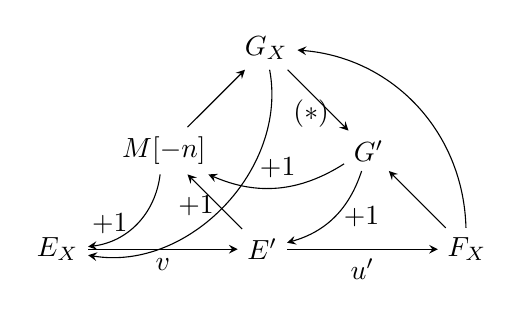
\begin{tikzpicture}[>=stealth,baseline=(GX.base),node distance=1.0cm]
  \node (EX) at (0,0) {$E_X$};
  \node (Ep) at (2.6,0) {$E'$};
  \node (FX) at (5.2,0) {$F_X$};
  \node (M)  at (1.35,1.25) {$M[-n]$};
  \node (GX) at (2.65,2.55) {$G_X$};
  \node (Gp) at (3.95,1.25) {$G'$};
  \node at (3.22,1.72) {$(*)$};
  \draw[->] (EX) -- node[below] {$v$} (Ep);
  \draw[->] (Ep) -- node[below] {$u'$} (FX);
  \draw[->] (Ep) -- (M);
  \draw[->] (M) -- (GX);
  \draw[->] (GX) -- (Gp);
  \draw[->] (FX) -- (Gp);
  \draw[->] (M) to[bend left=38] node[left] {$+1$} (EX);
  \draw[->] (Gp) to[bend left=28] node[above] {$+1$} (M);
  \draw[->] (Gp) to[bend left=28] node[right] {$+1$} (Ep);
  \draw[->] (GX) to[bend left=55] node[left] {$+1$} (EX);
  \draw[->] (FX) to[bend right=42] (GX);
\end{tikzpicture}
\]
The exact cohomology sequence of the distinguished triangle marked by the octahedron shows that
\[
  \Ho^n(G_X)\longrightarrow \Ho^n(G')
\]
is an epimorphism; hence \(\Ho^n(G')\) is indeed of \(\mathcal C_0\)-finite type.

The preceding correction therefore reduces us to the case where \(\Ho^{n+1}(u)\) is a monomorphism. We suppose this from now on. The exact cohomology sequence of \(E\to F\to G\) then gives an exact sequence
\[
  \Ho^n(E)\xrightarrow{\Ho^n(u)}
  \Ho^n(F)\longrightarrow \Ho^n(G)\longrightarrow 0.
\]
Since \(\Ho^n(G)\) is of \(\mathcal C_0\)-finite type, the set of \(X\) over \(S\) for which there exists an epimorphism
\[
  M\longrightarrow \Ho^n(G_X),\qquad M\in\Ob\mathcal C_{0,X},
\]
is, by definition, a refinement of \(S\). Using the quasi-liftability of \(\mathcal C_0\) in \(\mathcal C\), one may impose that this epimorphism factor through \(Z^n(F_X)\):
\[
  M\xrightarrow{s}Z^n(F_X)\longrightarrow \Ho^n(F_X)\longrightarrow \Ho^n(G_X).
\]
It is clear that \(u'\), defined as in (1.4.1) with \(r=0\), is a morphism of complexes and that
\[
  \Ho^n(u'):\Ho^n(E_X)\oplus M\longrightarrow \Ho^n(F_X)
\]
is an epimorphism. This completes the proof of (1.4.1).

\textbf{Lemma 1.4.2.} Let \(\mathcal C\) be an abelian category, let \(u:E\to F\) be a morphism of complexes of \(\mathcal C\) (respectively an arrow of \(\Dpx(\mathcal C)\)), and let \(G\) be the cone of \(u\). For a given \(n\in\mathbb Z\), the following conditions are equivalent:
\begin{enumerate}[label=(\roman*)]
\item \(\Ho^i(G)=0\) for \(i\geq n\);
\item \(\Ho^i(u)\) is an isomorphism for \(i>n\) and an epimorphism for \(i=n\).
\end{enumerate}
The proof is immediate from the exact cohomology sequence.

\textbf{Definition 1.4.3.} We shall say that \(u\) is an \(n\)-\emph{quasi-isomorphism} (respectively an \(n\)-\emph{isomorphism}) if \(u\) satisfies the equivalent conditions of (1.4.2).

That being so, one deduces at once from (1.4.1) the following:

\textbf{Corollary 1.4.4.} Let \(S,S,\mathcal C,\mathcal C_0\) be as in (1.4.1). Let \(u:E\to F\) be an \((n+1)\)-quasi-isomorphism of complexes of \(\mathcal C_S\), with \(n\in\mathbb Z\) fixed, such that \(\Ho^n(G)\) is of \(\mathcal C_0\)-finite type. Then the set of \(X\) over \(S\) for which there exist \((M,r,s)\) as in (1.4.1) such that \(u'\) is an \(n\)-quasi-isomorphism is a refinement of \(S\).

In pictorial terms, one may, using the finiteness condition on \(\Ho^n(G)\), locally ``gain one notch,'' that is, locally modify \(u\) in degree \(n\) by adding to \(E^n\) an object of \(\mathcal C_0\) in such a way as to make \(u\) an \(n\)-quasi-isomorphism.

\textbf{Corollary 1.4.5.} Let \(\mathcal C\) be an abelian category, let \(n\in\mathbb Z\), and let \(u:E\to F\) be an \(n\)-quasi-isomorphism of complexes of \(\mathcal C\). There exists a commutative diagram in \(\Cpx(\mathcal C)\)
\[
\begin{tikzcd}
E \arrow[r,"v"] \arrow[d,"u"'] & E' \arrow[dl,"u'"]\\
F &
\end{tikzcd}
\]
where \(u'\) is a quasi-isomorphism and \(v\) is a monomorphism inducing the identity in degrees \(\geq n\), that is,
\[
  E'^i=E^i,\qquad v^i=\id(E^i)\qquad\text{for }i\geq n.
\]

\emph{Proof.} Applying (1.4.4) in the case where \(S\) is the punctual site and \(\mathcal C_0=\mathcal C\), one obtains a commutative triangle in \(\Cpx(\mathcal C)\)
\[
\begin{tikzcd}
E \arrow[r,"v_{n-1}"] \arrow[d,"u"'] & E'_{\,n-1} \arrow[dl,"u'_{n-1}"]\\
F &
\end{tikzcd}
\]
where \(u'_{n-1}\) is an \((n-1)\)-quasi-isomorphism and \(v_{n-1}\) is a monomorphism inducing the identity in degrees \(\geq n\). Iterating the process, one finds, for \(i\leq n-1\), a sequence of commutative triangles in \(\Cpx(\mathcal C)\)
\[
\begin{tikzcd}
E'_i \arrow[r,"v_{i-1}"] \arrow[d,"u'_i"'] & E'_{\,i-1} \arrow[dl,"u'_{i-1}"]\\
F &
\end{tikzcd}
\]
where \(u'_i\) is an \(i\)-quasi-isomorphism and \(v_{i-1}\) is a monomorphism inducing the identity in degrees \(\geq i\). The corollary follows by passing to the limit. More precisely, writing \(d'_i\) for the differential of \(E'_i\), define \(E'\) by
\[
  E'^i=E^i,\quad d'^i=d^i\quad (i\geq n),
\]
and
\[
  E'^i=(E'_i)^i,\quad d'^i=(d'_i)^i\quad (i<n),
\]
and then define \(v\) and \(u'\) by
\[
  v^j=(v_i)^j,\qquad u'^j=(u'_i)^j\qquad (i\leq j).
\]
One immediately verifies that \(E'\), \(v\), and \(u'\), so defined, answer the question.

In abbreviated form: one can extend an \(n\)-quasi-isomorphism into a quasi-isomorphism ``without changing anything given in degree \(>n\).''

\section*{2. Pseudo-coherent complexes}

\textbf{2.0.} In this section, \(S\) denotes a site, \(S\) an object of \(S\), \(\mathcal C\) a flat abelian \(S\)-category (1.1), and \(\mathcal C_0\) a strictly full additive sub-\(S\)-category of \(\mathcal C\). We assume that \(\mathcal C_0\) is locally quasi-stable under kernels of epimorphisms (1.2) and locally quasi-liftable in \(\mathcal C\) (1.2).

\textbf{Definition 2.1.} Let \(X\in\Ob S\), let \(E\) be a complex of \(\mathcal C_X\), and let \(n\in\mathbb Z\). We shall say that \(E\) is \emph{strictly \(\mathcal C_0\)-\(n\)-pseudo-coherent} (respectively \(\mathcal C_0\)-pseudo-coherent, respectively \(\mathcal C_0\)-perfect) if \(E^i=0\) for \(i\) sufficiently large and \(E^i\in\Ob\mathcal C_{0,S}\) for \(i\geq n\) (respectively for every \(i\), respectively for every \(i\) and \(E^i=0\) for almost all \(i\)).

When no confusion is to be feared, we shall sometimes say ``strictly \(n\)-pseudo-coherent'' (respectively, and so on) instead of ``strictly \(\mathcal C_0\)-\(n\)-pseudo-coherent''.

\textbf{Lemma 2.1.1.} Let \(E\in\Ob\Cpx(\mathcal C_S)\) and \(n\in\mathbb Z\). If \(E\) is strictly \(n\)-pseudo-coherent and if \(\Ho^i(E)=0\) for \(i>n\), then \(\Ho^n(E)\) is of finite type.

\emph{Proof.} The sequence
\[
  0\longrightarrow Z^n(E)\longrightarrow E^n\longrightarrow E^{n+1}\longrightarrow\cdots\longrightarrow 0
\]
is exact, and \(E^i\in\Ob\mathcal C_0\) for \(i\geq n\). Since \(\mathcal C_0\) is locally quasi-stable under kernels of epimorphisms, it follows that \(Z^n(E)\) is of finite type, hence so is \(\Ho^n(E)\), which is a quotient of it.

\textbf{Proposition 2.2.} Let \(F\in\Ob\Dpx(\mathcal C_S)\) and \(n\in\mathbb Z\). Then:

\textbf{a)} If \(F\) is strictly \(n\)-pseudo-coherent (relative to \(\mathcal C_0\)) and if
\[
  u:E\longrightarrow F
\]
is a quasi-isomorphism, then the set of \(X\) over \(S\) such that there exists a quasi-isomorphism
\[
  v:F'\longrightarrow E_X
\]
with \(F'\) strictly \(n\)-pseudo-coherent is a refinement of \(S\).

\textbf{b)} The following conditions are equivalent:
\begin{enumerate}[label=(\roman*)]
\item the set of \(X\) over \(S\) such that there exists a quasi-isomorphism
\[
  u:E\longrightarrow F_X
\]
of \(\Cpx(\mathcal C_X)\), with \(E\) strictly \(n\)-pseudo-coherent, is a refinement of \(S\);
\item[\((\mathrm{i}')\)] the same condition as (i), but with \(u\) an isomorphism of \(\Dpx(\mathcal C_X)\);
\item the set of \(X\) over \(S\) such that there exists an \(n\)-quasi-isomorphism
\[
  u:E\longrightarrow F_X
\]
of \(\Cpx(\mathcal C_X)\), with \(E\) strictly perfect, is a refinement of \(S\);
\item[\((\mathrm{ii}')\)] the same condition as (ii), but with \(u\) an \(n\)-isomorphism of \(\Dpx(\mathcal C_X)\).
\end{enumerate}

\emph{Proof.} For a), there exists, for \(i\) sufficiently large, an \(i\)-quasi-isomorphism
\[
  v_i:F'_i\longrightarrow E
\]
with \(F'_i\) strictly \(n\)-pseudo-coherent (take \(F'_i=0\)). We show that, if \(i>n\), there exists, after refining \(S\), an \((i-1)\)-quasi-isomorphism
\[
  v_{i-1}:F'_{i-1}\longrightarrow E
\]
with \(F'_{i-1}\) strictly \(n\)-pseudo-coherent. By (1.4.4), it is enough to show that \(\Ho^{i-1}(M')\), where \(M'\) is the cone of \(v_i\), is of \(\mathcal C_0\)-finite type. Now if \(M''\) denotes the cone of \(uv_i\), the hypothesis that \(u\) is a quasi-isomorphism and (1.4.2) imply that
\[
  \Ho^j(M')\qis \Ho^j(M'')\qquad\text{for all }j,
\]
and
\[
  \Ho^j(M')=0\qquad\text{for }j\geq i.
\]
The cone formula
\[
  M''{}^j=F'_i{}^{\,j+1}\oplus F^j
\]
shows, on the other hand, that \(M''\) is strictly \((i-1)\)-pseudo-coherent. Hence, by (2.1.1),
\[
  \Ho^{i-1}(M'')=\Ho^{i-1}(M')
\]
is of finite type, whence the assertion. It follows, by iteration and after refining \(S\), that there is an \(n\)-quasi-isomorphism
\[
  v_n:F'_n\longrightarrow E
\]
where \(F'_n\) is strictly \(n\)-pseudo-coherent. But, by (1.4.5), one can extend \(v_n\) into a quasi-isomorphism
\[
  v:F'\longrightarrow E
\]
without changing anything in degrees \(\geq n\); in particular \(F'\) is strictly \(n\)-pseudo-coherent. This proves a).

For b), the equivalence of (i) and \((\mathrm{i}')\) follows at once from a) and from the definition of isomorphisms of \(\Dpx^-(\mathcal C_X)\). If \(E\in\Ob\Dpx^-(\mathcal C_S)\) is strictly \(n\)-pseudo-coherent, there is an exact sequence
\[
  0\longrightarrow E'\longrightarrow E\longrightarrow E''\longrightarrow 0
\]
where \(E'\) is strictly perfect and \(E''{}^i=0\) for \(i\geq n\). Consequently \(E'\to E\) is an \(n\)-quasi-isomorphism, which gives the implication \((\mathrm{i})\Rightarrow(\mathrm{ii})\). The implication \((\mathrm{ii})\Rightarrow(\mathrm{ii}')\) is trivial, so it remains to prove \((\mathrm{ii}')\Rightarrow(\mathrm{i})\). Let
\[
  u:E\longrightarrow F
\]
be an \(n\)-isomorphism of \(\Dpx^-(\mathcal C_S)\), with \(E\) strictly perfect. Then \(u\) is represented by a diagram in \(\Cpx^-(\mathcal C_S)\)
\[
\begin{tikzcd}
& E' \arrow[dl,"s"'] \arrow[dr,"u'"]\\
E && F ,
\end{tikzcd}
\]
where \(s\) is a quasi-isomorphism and \(u'\) an \(n\)-quasi-isomorphism. By a), after refining \(S\), there exists a quasi-isomorphism
\[
  t:E''\longrightarrow E',
\]
with \(E''\) strictly \(n\)-pseudo-coherent. Applying (1.4.5) to \(u't:E''\to F\), we extend it to a quasi-isomorphism
\[
  E'''\longrightarrow F
\]
with \(E'''\) strictly \(n\)-pseudo-coherent. This proves \((\mathrm{ii}')\Rightarrow(\mathrm{i})\) and completes the proof of (2.2).

\textbf{Definition 2.3.} Under the hypotheses of (2.2), we shall say that \(F\in\Ob\Dpx^-(\mathcal C_S)\) is \(n\)-\(\mathcal C_0\)-pseudo-coherent if \(F\) satisfies the equivalent conditions b) of (2.2). We shall say that \(F\) is \(\mathcal C_0\)-pseudo-coherent if \(F\) is \(n\)-\(\mathcal C_0\)-pseudo-coherent for every \(n\).

When this cannot cause confusion, we shall sometimes allow ourselves to say \(n\)-pseudo-coherent, pseudo-coherent, instead of \(n\)-\(\mathcal C_0\)-pseudo-coherent, \(\mathcal C_0\)-pseudo-coherent.

\textbf{Remark 2.3.1.} Let \(F\in\Ob\Dpx(\mathcal C_S)\) be a pseudo-coherent complex. The set of \(X\) over \(S\) such that there exists a quasi-isomorphism
\[
  E\longrightarrow F_X
\]
with \(E\) strictly pseudo-coherent (2.1) is not in general a refinement of \(S\). However, we shall see later (2.7 a) and Exposé II) important cases in which this is so.

The proof of (2.2 a) gives the following result.

\textbf{Proposition 2.4.} Let \(n,i\in\mathbb Z\), and let
\[
  u:E\longrightarrow F
\]
be an \(i\)-quasi-isomorphism of \(\Cpx(\mathcal C_S)\), with \(F\) \(n\)-pseudo-coherent and \(E\) strictly \(n\)-pseudo-coherent. Then, after refining \(S\), there exists a commutative triangle in \(\Cpx(\mathcal C_S)\)
\[
\begin{tikzcd}
E \arrow[r,"v"] \arrow[d,"u"'] & E' \arrow[dl,"u'"]\\
F &
\end{tikzcd}
\]
where \(E'\) is strictly \(n\)-pseudo-coherent, \(u'\) is a quasi-isomorphism, and \(v\) is a monomorphism inducing the identity in degree \(\geq i\).

\textbf{Proposition 2.5.} \textbf{a)} If \(F\in\Ob\Dpx(\mathcal C_S)\) is \(n\)-pseudo-coherent (respectively pseudo-coherent), then \(F[m]\) is \((n-m)\)-pseudo-coherent (respectively pseudo-coherent).

\textbf{b)} Let
\[
\begin{tikzcd}
E \arrow[rr] && F \arrow[dl]\\
& G \arrow[ul,"+1"] &
\end{tikzcd}
\tag{*}
\]
be a distinguished triangle of \(\Dpx(\mathcal C_S)\). If \(E\) and \(G\) are \(n\)-pseudo-coherent (respectively pseudo-coherent), then \(F\) is \(n\)-pseudo-coherent (respectively pseudo-coherent).

\emph{Proof.} a) is trivial from the definitions.

b) It is enough, of course, to prove the non-parenthesized assertion. The triangle \((*)\) can also be written
\[
\begin{tikzcd}
G[-1] \arrow[rr] && E \arrow[dl]\\
& F \arrow[ul,"+1"] &
\end{tikzcd}
\]
By a), \(G[-1]\) is \((n+1)\)-pseudo-coherent. Thus we are reduced to proving that, if \(E\) is \((n+1)\)-pseudo-coherent and \(F\) is \(n\)-pseudo-coherent, then \(G\) is \(n\)-pseudo-coherent. After localizing, we may assume \(E\) (respectively \(F\)) strictly \((n+1)\)-pseudo-coherent (respectively \(n\)-pseudo-coherent). The arrow
\[
  E\xrightarrow{u}F
\]
of \(\Dpx^-(\mathcal C_S)\) is represented by a pair of arrows of \(\Cpx^-(\mathcal C_S)\)
\[
\begin{tikzcd}
& E' \arrow[dl,"s"'] \arrow[dr,"u'"]\\
E && F ,
\end{tikzcd}
\]
where \(s\) is a quasi-isomorphism. By (2.2 a)), after localizing, there exists a quasi-isomorphism
\[
  t:E''\longrightarrow E',
\]
where \(E''\) is strictly \((n+1)\)-pseudo-coherent. We are therefore reduced to the case where \(u\) is defined by a true arrow of \(\Cpx^-(\mathcal C_S)\). The assertion then follows from the definitions and from the formula
\[
  C(u)^i=E^{i+1}\oplus F^i,
\]
where \(C(u)\) denotes the cone of \(u\).

\textbf{Scholium 2.6.} By rotation of triangles, one sees that pseudo-coherence properties for two of the objects of the triangle \((*)\) imply another such property for the third. The various cases may be summarized in the table below; the lower-case letters denote degrees of pseudo-coherence, and in each row the conclusion is underlined:
\[
\begin{array}{ccc}
E&F&G\\[0.2em]
n+1&n&\underline n\\
n&\underline n&n\\
\underline n&n&n-1 .
\end{array}
\]

We shall write
\[
  \Dpx(\mathcal C)_{\mathcal C_0\text{-}n\mathrm{coh}}
  \quad\text{respectively}\quad
  \Dpx(\mathcal C)_{\mathcal C_0\text{-}\mathrm{coh}}
\]
for the strictly full fibered subcategory of \(\Dpx(\mathcal C)\) whose fiber over each \(X\in\Ob S\) is formed by the objects of \(\Dpx(\mathcal C_X)\) that are \(n\)-pseudo-coherent (respectively pseudo-coherent) relative to \(\mathcal C_0\). By (2.5), the category
\[
  \Dpx(\mathcal C)_{\mathcal C_0\text{-}\mathrm{coh}}
\]
is a triangulated sub-\(S\)-category of \(\Dpx(\mathcal C)\) (1.1).

\textbf{Proposition 2.7.} Suppose that \(S\) is the punctual site, so that
\[
  \mathcal C=\mathcal C_S,\qquad \mathcal C_0=\mathcal C_{0,S}.
\]
Then:
\begin{enumerate}[label=\alph*)]
\item If \(F\in\Ob\Dpx(\mathcal C)\) is pseudo-coherent, there exists a quasi-isomorphism
\[
  E\longrightarrow F
\]
with \(E\) strictly pseudo-coherent (2.1).
\item Let \(\Kpx^{-,\mathrm{ac}}(\mathcal C_0)\) denote the full triangulated subcategory of \(\Kpx^-(\mathcal C_0)\) formed by acyclic complexes. The canonical functor
\[
  \Kpx^-(\mathcal C_0)/\Kpx^{-,\mathrm{ac}}(\mathcal C_0)
  \longrightarrow \Dpx(\mathcal C)
\]
is fully faithful and has essential image \(\Dpx(\mathcal C)_{\mathcal C_0\text{-}\mathrm{coh}}\).
\end{enumerate}

\emph{Proof.} a) Let \(F\in\Ob\Dpx(\mathcal C)_{\mathcal C_0\text{-}\mathrm{coh}}\), and suppose constructed an \(i\)-quasi-isomorphism
\[
  u_i:E_i\longrightarrow F
\]
of \(\Cpx(\mathcal C)\), with \(E_i\) strictly pseudo-coherent; this is possible for \(i\) sufficiently large, taking \(E_i=0\). Let \(G_i\) be the cone of \(u_i\). It follows from (1.4.2) and (2.1.1) that \(\Ho^{i-1}(G_i)\) is of \(\mathcal C_0\)-finite type. Hence, by (1.4.4), there exists a commutative triangle in \(\Cpx(\mathcal C)\)
\[
\begin{tikzcd}
E_i \arrow[r,"v_{i-1}"] \arrow[d,"u_i"'] & E_{i-1} \arrow[dl,"u_{i-1}"]\\
F &
\end{tikzcd}
\]
where \(E_{i-1}\) is strictly pseudo-coherent, \(u_{i-1}\) an \((i-1)\)-quasi-isomorphism, and \(v_{i-1}\) a monomorphism inducing the identity in degrees \(\geq i\). Passing to the limit (cf. the proof of (1.4.5)) gives a quasi-isomorphism
\[
  u:E\longrightarrow F
\]
with \(E\) strictly pseudo-coherent.

b) Apply the criterion of \([V]\), Chap. I, §2, 4.2 b)(i), together with a).

We note that the proof of a) gives the following more precise result, which generalizes (1.4.5).

\textbf{Proposition 2.7.1.} Under the hypotheses of (2.7), let \(u:E\to F\) be an \(n\)-quasi-isomorphism of \(\Cpx(\mathcal C)\), with \(F\) pseudo-coherent and \(E\) strictly pseudo-coherent. Then there exists a commutative triangle in \(\Cpx(\mathcal C)\)
\[
\begin{tikzcd}
E \arrow[r,"v"] \arrow[d,"u"'] & E' \arrow[dl,"u'"]\\
F &
\end{tikzcd}
\]
where \(E'\) is strictly pseudo-coherent, \(u'\) is a quasi-isomorphism, and \(v\) is a monomorphism inducing the identity in degree \(\geq n\).

\textbf{Definition 2.8.} Let \(n\in\mathbb N\) and \(F\in\Ob\mathcal C_S\). We shall say that \(F\) is of \(n\)-\(\mathcal C_0\)-finite presentation if the set of \(X\) over \(S\) such that there exists an exact sequence
\[
  E^{-n}\longrightarrow\cdots\longrightarrow E^0\longrightarrow F_X\longrightarrow 0,
\qquad E^i\in\Ob\mathcal C_{0,X}\quad(-n\leq i\leq 0),
\]
is a refinement of \(S\). We shall say that \(F\) is of \(\infty\)-\(\mathcal C_0\)-finite presentation if \(F\) is of \(n\)-\(\mathcal C_0\)-finite presentation for every \(n\in\mathbb N\).

Of course, we shall sometimes simply say \(n\)-finite presentation when there is no possible ambiguity about \(\mathcal C_0\). We shall say ``finite presentation'' for ``1-finite presentation,'' and ``finite type'' for ``0-finite presentation,'' the latter notion coinciding with the one already introduced in (1.2).

\textbf{Proposition 2.9.} Let \(n\in\mathbb N\) and \(F\in\Ob\mathcal C_S\). The following conditions are equivalent:
\begin{enumerate}[label=(\roman*)]
\item \(F\) is of \(n\)-finite presentation (respectively of \(\infty\)-finite presentation);
\item \(F\) is \((-n)\)-pseudo-coherent (respectively pseudo-coherent).
\end{enumerate}
In the case where \(S\) is the punctual site, \(F\) is pseudo-coherent if and only if there exists an exact sequence
\[
  \cdots\longrightarrow E^i\longrightarrow\cdots\longrightarrow E^0\longrightarrow F\longrightarrow 0,
\qquad E^i\in\Ob\mathcal C_0\quad\text{for all }i.
\]

\emph{Proof.} For the equivalence \((\mathrm{i})\Leftrightarrow(\mathrm{ii})\), it is plainly enough to treat the non-parenthesized case. The implication \((\mathrm{i})\Rightarrow(\mathrm{ii})\) is immediate from the definitions, and \((\mathrm{ii})\Rightarrow(\mathrm{i})\) follows at once from (2.4): the arrow \(0\to F\) is a \(1\)-quasi-isomorphism, and from this one deduces, after localizing, a quasi-isomorphism
\[
  E\longrightarrow F
\]
with \(E\) strictly \((-n)\)-pseudo-coherent and \(E^i=0\) for \(i\geq 1\), that is, an \(n\)-finite presentation of \(F\). The second assertion is proved in the same way, using (2.7.1).

\textbf{Proposition 2.10.} \textbf{a)} Let \(m,n\in\mathbb Z\), with \(n\leq m\). If \(F\in\Ob\Dpx^-(\mathcal C_S)\) is \(n\)-pseudo-coherent and acyclic in degrees \(\geq m\), then there exists locally a quasi-isomorphism
\[
  E\longrightarrow F
\]
with \(E\) strictly \(n\)-pseudo-coherent and \(E^i=0\) for \(i\geq m\). If \(S\) is punctual, and if \(F\) is pseudo-coherent and acyclic in degrees \(\geq m\), there exists a quasi-isomorphism
\[
  E\longrightarrow F
\]
with \(E\) strictly pseudo-coherent and \(E^i=0\) for \(i\geq m\).

\textbf{b)} Let \(F\in\Ob\Dpx^-(\mathcal C_S)\) be acyclic in degrees \(>n\). For \(F\) to be \(n\)-pseudo-coherent, it is necessary and sufficient that \(\Ho^n(F)\) be of finite type.

\emph{Proof.} a) Since \(F\) is acyclic in degrees \(\geq m\), the arrow \(0\to F\) is an \(m\)-quasi-isomorphism. The assertion follows from (2.4) and (2.7.1).

b) There exists a distinguished triangle in \(\Dpx^-(\mathcal C_S)\):
\[
\begin{tikzcd}
F \arrow[rr] && F' \arrow[dl]\\
& \Ho^n(F)[-n] \arrow[ul,"+1"] &
\end{tikzcd}
\]
(to see this, begin by truncating \(F\), replacing \(F^n\) by \(Z^n(F)\) and \(F^i\) by \(0\) for \(i>n\)). The exact cohomology sequence implies
\[
  \Ho^i(F')=0\quad\text{for }i\geq n-1,
\]
so \(F'\) is \((n-1)\)-pseudo-coherent. We conclude by (2.5) and (2.6).



% Additional notation for Expose I continuation
\providecommand{\RHom}{\mathrm R\!\Hom}
\providecommand{\Ext}{\operatorname{Ext}}
\providecommand{\coh}{\operatorname{coh}}
\providecommand{\PreCoh}{\operatorname{precoh}}
\providecommand{\Tr}{\operatorname{Tr}}
\providecommand{\Qis}{\operatorname{Qis}}
\providecommand{\Rad}{\operatorname{rad}}
\providecommand{\Spec}{\operatorname{Spec}}
\providecommand{\End}{\operatorname{End}}
\providecommand{\Id}{\operatorname{Id}}
\providecommand{\varinjlim}{\mathop{\mathrm{lim}}\limits_{\longrightarrow}}
\providecommand{\varprojlim}{\mathop{\mathrm{lim}}\limits_{\longleftarrow}}
\providecommand{\qcoh}{\operatorname{qcoh}}
\providecommand{\amp}{\operatorname{amp}}


\section*{Exposé I, continued: pseudo-coherent complexes and perfect complexes}

\textbf{Proposition 2.11.} Let \(n\in\mathbb Z\).

\textbf{a)} Let \(F\in\Ob\Cpx^-(\mathcal C_S)\). If, for every \(i\geq n\) (respectively for every \(i\)), \(F^i\) is of finite \((i-n)\)-presentation (respectively of finite \(\infty\)-presentation), then \(F\) is \(n\)-pseudo-coherent (respectively pseudo-coherent).

\textbf{b)} Let \(F\in\Ob\Dpx^-(\mathcal C_S)\). If, for every \(i\geq n\) (respectively for every \(i\)), \(\Ho^i(F)\) is of finite \((i-n)\)-presentation (respectively of finite \(\infty\)-presentation), then \(F\) is pseudo-coherent.

\emph{Proof.} It is enough to treat the non-parenthesized assertions.

\textbf{a)} We argue by induction on \(N\) such that \(F^i\neq0\) only for \(i\leq n+N\). If \(N=0\), the assertion follows at once from (2.10 b). Suppose \(N\geq1\). We have an exact sequence
\[
  0\longrightarrow F^{n+N}[-n-N]\longrightarrow F\longrightarrow F'\longrightarrow 0 .
\]
By the induction hypothesis, \(F'\) is \(n\)-pseudo-coherent; on the other hand \(F^{n+N}[-n-N]\) is \(n\)-pseudo-coherent by hypothesis, using (2.9 and 2.5 a). Hence, by (2.5 b), \(F\) is \(n\)-pseudo-coherent.

\textbf{b)} We argue by induction on \(N\) such that \(\Ho^i(F)=0\) for \(i>n+N\). If \(N=0\), the assertion follows from (2.10 b). Suppose \(N\geq1\). As in the proof of (2.10 b), we have a distinguished triangle in \(\Dpx^-(\mathcal C_S)\)
\[
  F'\longrightarrow F\longrightarrow \Ho^{n+N}(F)[-n-N]\longrightarrow F'[1].
\]
more plainly, with cone \(\Ho^{n+N}(F)[-n-N]\). The exact cohomology sequence implies
\[
  \Ho^i(F')=0\quad\text{for } i>n+N-1,
\]
that is, for \(i>(n-1)+(N-1)\), and
\[
  \Ho^i(F')\qis \Ho^{i+1}(F)\quad\text{for }i<n+N-1 .
\]
By the induction hypothesis, applied with \(n-1\) in place of \(n\), \(F'\) is therefore \((n-1)\)-pseudo-coherent. On the other hand, \(\Ho^{n+N}(F)[-n-N]\) is \(n\)-pseudo-coherent by (2.9 and 2.5 a). Hence, by (2.6), \(F\) is \(n\)-pseudo-coherent.

\textbf{Remark 2.11.1.} If \(F\) is pseudo-coherent, the \(F^i\) (respectively the \(\Ho^i(F)\)) are not in general pseudo-coherent, nor even of finite type. Nevertheless, in the following paragraph, in the excursions on the notions of coherence, we shall see important examples where pseudo-coherence of \(F\) implies that of the \(\Ho^i(F)\).

\textbf{Proposition 2.12.} Let \(F',F''\in\Ob\Dpx^-(\mathcal C_S)\), and let \(F=F'\oplus F''\). For \(F\) to be \(n\)-pseudo-coherent (respectively pseudo-coherent), it is necessary and sufficient that \(F'
\) and \(F''\) be \(n\)-pseudo-coherent (respectively pseudo-coherent).

\emph{Proof.} It is enough to prove the non-parenthesized assertion. Sufficiency is obvious; let us prove necessity. By induction we may suppose that it has already been proved that \(F'\) and \(F''\) are \((n+1)\)-pseudo-coherent. After localizing, we may even suppose that \(F'\) and \(F''\) are strictly \((n+1)\)-pseudo-coherent and that \(F=F'\oplus F''\) in \(\Cpx^-(\mathcal C_S)\). Let \(F'_{>n}\) (respectively \(F'_{\leq n}\)) denote the complex obtained from \(F'\) by replacing \(F'^i\) by \(0\) for \(i\leq n\) (respectively for \(i>n\)), and define \(F''_{>n}\) and \(F''_{\leq n}\) similarly. We have an exact sequence
\[
  0\longrightarrow F'_{>n}\oplus F''_{>n}\longrightarrow F
  \longrightarrow F'_{\leq n}\oplus F''_{\leq n}\longrightarrow 0 .
\]
The complex \(F'_{>n}\oplus F''_{>n}\) is strictly perfect; since \(F\) is \(n\)-pseudo-coherent, (2.6) implies that \(F'_{\leq n}\oplus F''_{\leq n}\) is \(n\)-pseudo-coherent. This means, by (2.10 b), that
\[
  \Ho^n(F'_{\leq n}\oplus F''_{\leq n})
\]
is of finite type. But
\[
  \Ho^n(F'_{\leq n}\oplus F''_{\leq n})
  =\Ho^n(F'_{\leq n})\oplus \Ho^n(F''_{\leq n}),
\]
so \(\Ho^n(F'_{\leq n})\) (respectively \(\Ho^n(F''_{\leq n})\)) is of finite type, and again by (2.10 b) \(F'_{\leq n}\) (respectively \(F''_{\leq n}\)) is \(n\)-pseudo-coherent. Applying (2.5) to the exact sequence
\[
  0\longrightarrow F'_{>n}\longrightarrow F'\longrightarrow F'_{\leq n}\longrightarrow 0
\]
(and similarly for \(F''\)), we deduce that \(F'\) and \(F''\) are \(n\)-pseudo-coherent.

\textbf{Proposition 2.13.} Let \((S',\mathcal C',\mathcal C'_0)\) be a triple satisfying the same hypotheses (2.0) as \((S,\mathcal C,\mathcal C_0)\). Let \(f:S'\to S\) be a morphism of sites, corresponding to an underlying functor \(f^{-1}:S\to S'\), and let
\[
  u:\Dpx^*(\mathcal C)\longrightarrow \Dpx^*(\mathcal C')\qquad (*=+,-,b)
\]
be a Cartesian functor above \(f\), exact on each fiber. Suppose that there exist \(a,b\in\mathbb Z\) such that, for every \(S\in\Ob S\), the following conditions hold:

\begin{enumerate}[label=(\roman*)]
\item if \(E\in\Ob\mathcal C_{0,S}\), then \(u(E)\) is \(a\)-\(\mathcal C'_0\)-pseudo-coherent (respectively \(\mathcal C'_0\)-pseudo-coherent);
\item if \(F\in\Ob\Dpx^*(\mathcal C_S)\) is acyclic in degrees \(>0\), then \(u(F)\) is acyclic in degrees \(>b\).
\end{enumerate}

Then, if \(F\in\Ob\Dpx^*(\mathcal C_S)\) is \(m\)-pseudo-coherent relative to \(\mathcal C_0\) and acyclic in degrees \(>n\), the object
\[
  u(F)\in\Ob\Dpx^*(\mathcal C'_{S'}),\qquad S'=f^{-1}(S),
\]
is \(\sup(m+b,n+a)\)-pseudo-coherent relative to \(\mathcal C'_0\) (respectively \((m+b)\)-pseudo-coherent), and is acyclic in degrees \(>n+b\). In particular, in the parenthesized case, if \(F\in\Ob\Dpx^*(\mathcal C_S)\) is pseudo-coherent relative to \(\mathcal C_0\), then \(u(F)\) is pseudo-coherent relative to \(\mathcal C'_0\).

\emph{Proof.} We may restrict to the non-parenthesized case. First suppose that \(F\in\Ob\Dpx^*(\mathcal C_S)\) is strictly perfect (2.1), with \(F^i=0\) for \(i>n\). Then \(u(F)\) is \((n+a)\)-\(\mathcal C'_0\)-pseudo-coherent. We argue by induction on the number \(N\) of indices \(i\) such that \(F^i\neq0\). If \(N=1\), then \(F=F^p[-p]\) for some \(p\leq n\), so \(u(F)\) is \((p+a)\)-\(\mathcal C'_0\)-pseudo-coherent, hence a fortiori \((n+a)\)-pseudo-coherent. If \(N>1\), there is an exact sequence
\[
  0\longrightarrow F'\longrightarrow F\longrightarrow F''\longrightarrow 0,
\]
where \(F'\) and \(F''\) are strictly perfect of length \(<N-1\), and where \(F'^i=F''^i=0\) for \(i>n\). Applying (2.5 b) to the distinguished triangle
\[
  u(F')\longrightarrow u(F)\longrightarrow u(F'')\longrightarrow u(F')[1].
\]
and using the induction hypothesis, we get that \(u(F)\) is \((n+a)\)-pseudo-coherent.

Now pass to the general case: \(F\) is \(m\)-\(\mathcal C_0\)-pseudo-coherent and acyclic in degrees \(>n\). After localizing, we may, by (2.10 a), suppose \(F\) strictly \(m\)-pseudo-coherent and such that \(F^i=0\) for \(i>n\). There is then an exact sequence
\[
  0\longrightarrow F'\longrightarrow F\longrightarrow F''\longrightarrow 0,
\]
where \(F''\) is zero in degrees \(\geq m\), and \(F'\) is strictly perfect and zero in degrees \(>n\). In the distinguished triangle
\[
  u(F')\longrightarrow u(F)\longrightarrow u(F'')\longrightarrow u(F')[1].
\]
the object \(u(F'')\) is acyclic in degrees \(>m+b\), hence \((m+b)\)-pseudo-coherent, while \(u(F')\) is \((n+a)\)-pseudo-coherent by what was just proved. We conclude by (2.5 b).

\textbf{Corollary 2.14.} Let \(\mathcal C_1\) be a strictly full additive sub-\(S\)-category of \(\mathcal C\) such that
\[
  \mathcal C_0\subset \mathcal C_1\subset \mathcal C.
\]
Assume that every object of \(\mathcal C_1\) is \(\mathcal C_0\)-pseudo-coherent. Then:

\begin{enumerate}[label=(\roman*)]
\item \(\mathcal C_1\) is locally quasi-liftable in \(\mathcal C\) (1.2), and locally quasi-stable under kernels of epimorphisms (1.2);
\item for \(S\in\Ob S\) and \(F\in\Ob\Dpx(\mathcal C_S)\), in order that \(F\) be \(n\)-pseudo-coherent (respectively pseudo-coherent) relative to \(\mathcal C_1\), it is necessary and sufficient that it be so relative to \(\mathcal C_0\).
\end{enumerate}

\emph{Proof.} For (i), let \(E\to F\) be an epimorphism in \(\mathcal C_S\), with \(F\in\Ob\mathcal C_{1,S}\). Since \(F\) is \(\mathcal C_0\)-pseudo-coherent, hence a fortiori of \(\mathcal C_0\)-finite type, there exists, after localizing, an epimorphism \(E'\to F\) with \(E'\in\Ob\mathcal C_{0,S}\). Using the quasi-liftability of \(\mathcal C_0\) in \(\mathcal C\), we may suppose, after localizing again, that this epimorphism factors through \(E\); this gives the quasi-liftability of \(\mathcal C_1\). On the other hand, if \(E\in\Ob\mathcal C_S\) admits a finite right resolution by objects of \(\mathcal C_1\), then \(E\) is \(\mathcal C_0\)-pseudo-coherent by (2.11 a), hence a fortiori of \(\mathcal C_1\)-finite type.

For (ii), it is enough to prove necessity. For this one may apply, at choice, (2.11 a) or (2.13), with \(S'=S\), \(\mathcal C'=\mathcal C\), \(f=\Id\), \(u=\Id\), and with \(\mathcal C'_0\) and \(\mathcal C_0\) replaced respectively by \(\mathcal C_0\) and \(\mathcal C_1\).

\textbf{Scholium 2.14.1.} There is therefore a largest strictly full additive sub-\(S\)-category of \(\mathcal C\) giving the same notion of \(n\)-pseudo-coherence (respectively pseudo-coherence) as \(\mathcal C_0\), namely the category formed by the \(\mathcal C_0\)-pseudo-coherent objects. This latter category is locally stable under kernels of epimorphisms.

\textbf{Example 2.15.} Let \((S,A)\) be a ringed topos, and let \(\mathcal C,\mathcal C_0\) be the \(S\)-categories considered in (1.3 d). The fibered category \(\Dpx(\mathcal C)\) will often be denoted by \(\Dpx(S,A)\), or \(\Dpx_A(S)\), when one wants to suggest that the modules are left \(A\)-modules, or even simply \(\Dpx(S)\) if there is no ambiguity about \(A\). We denote by \(S\) the final object of \(S\), and put \(\Dpx(\mathcal C_S)=\Dpx_A(S)\) (or \(\Dpx(S)\)). An object of \(\Dpx(S)\) will be said to be \(n\)-pseudo-coherent (respectively pseudo-coherent) if it is \(n\)-\(\mathcal C_0\)-pseudo-coherent (respectively \(\mathcal C_0\)-pseudo-coherent), and similarly for the strict notions. The category fibered in \(\Dpx(\mathcal C)\), denoted \(\Dpx(\mathcal C)_{n-\mathcal C_0-\coh}\) (respectively \(\Dpx(\mathcal C)_{\mathcal C_0-\coh}\)) in (2.6), will be denoted \(\Dpx_A(S)_{n-\coh}\) (respectively \(\Dpx_A(S)_{\coh}\)). One observes that, by (2.14), the same notion of pseudo-coherence is obtained if \(\mathcal C_0\) is replaced by the \(S\)-category \(\mathcal C_1\) defined by
\[
  U\longmapsto \text{the category of left }A_U\text{-modules locally direct summands of free finite-type modules}.
\]
If an \(A\)-module \(M\) is a direct summand of a free finite-type \(A\)-module, it does not follow in general that \(M\) is locally free of finite type. One does, however, have the following result.

\textbf{Lemma 2.15.1.} Suppose that \(S\) satisfies one of the following two hypotheses:
\begin{enumerate}[label=(\roman*)]
\item \(S\) has enough points (SGA 4 IV 6.4), and for every point \(s\) of \(S\), the left \(A_s\)-modules which are projective of finite type are free; this last condition is satisfied, for example, if \(A_s/\Rad(A_s)\) is a field or if \(\Rad(A_s)\) is nilpotent;
\item \((S,A)\) is a ``locally ringed'' topos in the sense of [1], which means that \(A\) is commutative and that, for every \(X\in\Ob S\) and every \(f\in\Gamma(X,A)\), one has
\[
  X=X_f\cup X_{1-f},
\]
where \(X_f\) (respectively \(X_{1-f}\)) denotes the largest subobject of \(X\) on which \(f\) (respectively \(1-f\)) is invertible.
\end{enumerate}
Then every direct summand of a free finite-type left \(A\)-module is locally free of finite type.

\emph{Proof.} Suppose first that (i) holds. We note that, if \(E\) and \(F\) are two \(A\)-modules and \(E\) is of finite presentation, the canonical arrow
\[
  \Hom(E,F)_s\longrightarrow \Hom(E_s,F_s)
\]
is an isomorphism for every point \(s\) of \(S\). It follows that, if \(E\) and \(F\) are both of finite presentation and if \(E_s\qis F_s\) at a point \(s\) of \(S\), then there is an \(s\)-pointed object \(U\) of \(S\) such that \(E|U\qis F|U\). The conclusion follows at once.

Suppose next that (ii) holds. Let \(n\in\mathbb N\), and let \(\mathbb D^n\) denote the functor on the category of locally ringed topoi belonging to a fixed universe, defined by
\[
  T\longmapsto \Gamma(T,\mathcal O_T)^n.
\]
It is known [1] that the functor \(\End_{\mathbb D}(\mathbb D^n)\) is represented by
\[
  M_n=\Spec\mathbb Z[T_{ij}]\quad(1\leq i\leq n,
  1\leq j\leq n),
\]
endowed with the endomorphism \(U_n\) of \((\mathcal O_{M_n})^n\) defined by the matrix \((T_{ij})\). Now let
\[
  p:A^n\longrightarrow A^n
\]
be a projector. We show that \(p(A^n)\) is locally free of finite type. From what has just been said, there exists a morphism
\[
  s:S\longrightarrow M_n
\]
of locally ringed topoi such that \(s^*(u_n)=p\). We may interpret \(s\) as a point of \(M_n\) with values in \(\Gamma(S,A)\), that is, as a matrix of order \(n\) with coefficients in \(\Gamma(S,A)\). Since this matrix is a projector, \(s\) factors through the closed subscheme
\[
  i:P_n\hookrightarrow M_n
\]
corresponding to projectors; say \(S\xrightarrow{s'}P_n\xrightarrow{i}M_n\). Hence
\[
  p=s'^* i^*(u_n),
\]
and we are done, because, by the assertion under hypothesis (i), the image of \(i^*(u_n)\) is a locally free finite-type sheaf.

\textbf{Corollary 2.16.} Let
\[
  f:(S',A')\longrightarrow (S,A)
\]
be a morphism of ringed topoi, defined by a functor \(f^{-1}:S\to S'\) and a morphism of sheaves of rings \(f^{-1}(A)\to A'\). Let \(\Dpx(_{A'}S'_A)\) denote the derived category of \(A'\)-\(A\)-bimodules, left over \(A'\) and right over \(A\), and let
\[
  \otimes_A^{\mathrm L}:\Dpx^-(_{A'}S'_A)\times_{S'}\Dpx^-(_A S)
  \longrightarrow \Dpx^-(_{A'}S')
\]
be the derived functor of the tensor product
\[
  (E',E)\longmapsto E'\otimes_A f^{-1}(E).
\]
Let \(X\in\Ob S\), put \(X'=u(X)\), and let \(E'\in\Ob\Dpx^-(_{A'}X'_A)\), \(E\in\Ob\Dpx^-(_A X)\). If \(E'\) is \(m'\)-pseudo-coherent (as an object of \(\Dpx^-(_A S')\)) and acyclic in degrees \(>n'\), and if \(E\) is \(m\)-pseudo-coherent and acyclic in degrees \(>n\), then
\[
  E'\otimes_A^{\mathrm L}E
\]
is \(\sup(m+n',m'+n)\)-pseudo-coherent and acyclic in degrees \(>n+n'\).

\emph{Proof.} After replacing \(S\) by \(S/X\), we may suppose \(X=S\), and apply (2.13) with
\[
  u=E'\otimes_A^{\mathrm L}:\Dpx^-(_A S)\longrightarrow \Dpx^-(_{A'}S').
\]
Let \(U\in\Ob S\), let \(U'=f^{-1}(U)\), and let \(E\) be a complex of left \(A_U\)-modules. If \(E\) is acyclic in degrees \(>n\), then \(E'\otimes_A^{\mathrm L}E\) is acyclic in degrees \(>n+n'\), by the definition of \(\otimes_A^{\mathrm L}\). On the other hand, if \(E=(A_U)^p\), then
\[
  E'\otimes_A^{\mathrm L}E=(E'|U')^p,
\]
which is \(m'\)-pseudo-coherent by hypothesis and (2.12). The conditions of (2.13) are therefore satisfied, with \(a=m'\) and \(b=n'\), whence the conclusion.

In particular:

\textbf{Corollary 2.16.1.} Under the hypotheses of (2.16), one has:

\textbf{a)} The functor
\[
  \mathrm L f^*: \Dpx^-(_A S)\longrightarrow \Dpx^-(_{A'}S')
\]
(which is none other than the functor \(A'\otimes_A^{\mathrm L}\)) induces a functor
\[
  \mathrm L f^*: \Dpx^-(_A S)_{\coh}\longrightarrow \Dpx^-(_{A'}S')_{\coh}
\]
(with the notation of (2.6)).

\textbf{b)} If \(A\) is commutative, the functor
\[
  \otimes_A^{\mathrm L}:\Dpx^-(S)\times_S\Dpx^-(S)
  \longrightarrow \Dpx^-(S)
\]
induces a functor
\[
  \otimes_A^{\mathrm L}:\Dpx^-(S)_{\coh}\times_S\Dpx^-(S)_{\coh}
  \longrightarrow \Dpx^-(S)_{\coh} .
\]

\textbf{Exercise 2.16.2.} Let \(S\) be a topos, and let \(A\to A'\) be a morphism of rings of \(S\). Assume one of the following hypotheses:
\begin{enumerate}[label=(\roman*)]
\item \(A\to A'\) is surjective, with nilpotent ideal as kernel;
\item the functor \(A'\otimes_A-\), on the category of left \(A\)-modules, is exact and faithful.
\end{enumerate}
Show that \(E\in\Ob\Dpx^-(_A S)\) is \(n\)-pseudo-coherent (respectively pseudo-coherent) if and only if
\[
  A'\otimes_A E\in\Ob\Dpx^-(_{A'}S)
\]
is \(n\)-pseudo-coherent (respectively pseudo-coherent).

Hints: first show that a left \(A\)-module \(L\) is of finite type if and only if \(A'\otimes_A L\) is of finite type (cf. Bourbaki, Commutative Algebra, Chap. I, §3, Prop. 11 and Chap. II, §3, Prop. 4), and then reduce to this case by truncation, using (2.5) and (2.10 b).

\section*{3. Link with the classical notion of coherence}

\textbf{3.0.} The hypotheses and notation are those of (2.0), except that \(\mathcal C_0\) is no longer assumed locally quasi-stable under kernels of epimorphisms.

\textbf{Definition 3.1.} Let \(F\in\Ob\mathcal C_S\). We shall say that \(F\) is \emph{precoherent} relative to \(\mathcal C_0\) if, for every \(U\) over \(S\) and every morphism
\[
  u:E\longrightarrow F|U,
\]
where \(E\in\Ob\mathcal C_{0,U}\), \(\Ker(u)\) is of \(\mathcal C_0\)-finite type (1.2). We shall say that \(F\) is \emph{coherent} relative to \(\mathcal C_0\) if \(F\) is precoherent and of finite type.

\emph{Technical note.} We introduce this notion here only as a technical intermediary; the only notion to retain is that of coherence.

\textbf{Remark 3.2.} Let \(F\in\Ob\mathcal C_S\). It is clear from the definitions that, if \(F\) is precoherent (respectively of finite type), then every subobject (respectively quotient) of \(F\) is precoherent (respectively of finite type).

\textbf{Lemma 3.3.}

\textbf{a)} Let
\[
  0\longrightarrow F\longrightarrow G\longrightarrow H
\]
be an exact sequence of \(\mathcal C_S\). If \(G\) is of finite type and \(H\) is precoherent, then \(F\) is of finite type.

\textbf{b)} Let
\[
  F\longrightarrow G\longrightarrow H\longrightarrow 0
\]
be an exact sequence of \(\mathcal C_S\). If \(F\) is of finite type and \(G\) is precoherent, then \(H\) is precoherent.

\textbf{c)} Let
\[
  0\longrightarrow F\longrightarrow G\longrightarrow H\longrightarrow 0
\]
be an exact sequence of \(\mathcal C_S\). If \(F\) and \(H\) are precoherent (respectively of finite type), then so is \(G\).

\emph{Proof.} a) After localizing, there is an epimorphism \(G'\to G\) with \(G'\in\Ob\mathcal C_0\). Hence there is a commutative diagram with exact rows
\[
\begin{tikzcd}
0\arrow[r]&F'\arrow[r]\arrow[d]&G'\arrow[r]\arrow[d]&H\arrow[d,"\Id"]\\
0\arrow[r]&F\arrow[r]&G\arrow[r]&H .
\end{tikzcd}
\]
Since \(H\) is precoherent, \(F'\) is of finite type; but \(F'\to F\) is an epimorphism, so \(F\) is of finite type.

b) Let \(U\) be over \(S\), and let \(H'\xrightarrow{f}H|U\) be a morphism of \(\mathcal C_U\), with \(H'\in\Ob\mathcal C_{0,U}\). After a change of notation, we may suppose \(U=S\). By the quasi-liftability of \(\mathcal C_0\) in \(\mathcal C\), there exists, after localizing, a commutative square
\[
\begin{tikzcd}
G' \arrow[r,"p"] \arrow[d] & H' \arrow[d,"f"]\\
G \arrow[r] & H,
\end{tikzcd}
\]
where the horizontal arrows are epimorphisms and \(G'\in\Ob\mathcal C_0\). Since \(\Ker(f)\) is a quotient of \(\Ker(fp)\), it is enough to show that \(\Ker(fp)\) is of finite type; hence we may suppose \(H'=G'\). The arrows \(F\to G\) and \(H'\to G\) define
\[
  g:F\oplus H'\longrightarrow G.
\]
Putting \(K=\Ker(G\to H)\), we have a commutative diagram, with exact rows and with \(q\) an epimorphism,
\[
\begin{tikzcd}
0\arrow[r]&F\arrow[r]\arrow[d,"q"]&F\oplus H'\arrow[r]\arrow[d,"g"]&H'\arrow[r]\arrow[d,"f"]&0\\
0\arrow[r]&K\arrow[r]&G\arrow[r]&H\arrow[r]&0 .
\end{tikzcd}
\]
The snake diagram shows that \(\Ker(g)\to\Ker(f)\) is an epimorphism. But, since \(F\oplus H'\) is of finite type and \(G\) is precoherent, \(\Ker(g)\) is of finite type by a); hence we are done.

c) First prove the non-parenthesized assertion. Up to a change of notation, it is a matter of showing that, if \(g:G'\to G\) is a morphism of \(\mathcal C_S\), with \(G'\in\Ob\mathcal C_0\), then \(\Ker(g)\) is of finite type. Let \(H'\) be the image of the composed arrow \(G'\to H\). We have a commutative diagram with exact rows
\[
\begin{tikzcd}
0\arrow[r]&F'\arrow[r]\arrow[d,"f"]&G'\arrow[r]\arrow[d,"g"]&H'\arrow[r]\arrow[d,"h"]&0\\
0\arrow[r]&F\arrow[r]&G\arrow[r]&H\arrow[r]&0 .
\end{tikzcd}
\]
Since \(h\) is a monomorphism, the snake diagram gives an isomorphism \(\Ker(f)\qis\Ker(g)\). But \(F'\) is of finite type by a), hence \(\Ker(f)\) is of finite type, again by a). This proves the non-parenthesized assertion. For the parenthesized assertion, strictly speaking one cannot invoke (2.5 b), since \(\mathcal C_0\) is not assumed locally quasi-stable under kernels of epimorphisms. After localizing, there are epimorphisms
\[
  F'\xrightarrow{u}F,
  \qquad H'\xrightarrow{v}H,
\]
with \(F',H'\in\Ob\mathcal C_0\). After localizing further, we may suppose that \(v\) factors through \(G\), whence a commutative diagram with exact rows
\[
\begin{tikzcd}
0\arrow[r]&F'\arrow[r]\arrow[d,"u"]&F'\oplus H'\arrow[r]\arrow[d,"w"]&H'\arrow[r]\arrow[d,"v"]&0\\
0\arrow[r]&F\arrow[r]&G\arrow[r]&H\arrow[r]&0 .
\end{tikzcd}
\]
Since \(u\) and \(v\) are epimorphisms, so is \(w\), and this proves the assertion. The proof of (3.3) is complete.

It follows immediately that:

\textbf{Corollary 3.4.} The full (respectively strictly full) subcategory of \(\mathcal C_S\) formed by coherent objects is stable under finite projective (respectively inductive) limits. In particular, the kernel, cokernel, and image of an arrow between two coherent objects are coherent. Let
\[
  E^0\longrightarrow E^1\longrightarrow E^2\longrightarrow E^3\longrightarrow E^4
\]
be an exact sequence of \(\mathcal C_S\). If \(E^0,E^1,E^3,E^4\) are coherent, then \(E^2\) is coherent as well.

\textbf{Corollary 3.5.} Suppose that the objects of \(\mathcal C_0\) are \(\mathcal C_0\)-coherent (which in particular implies that \(\mathcal C_0\) is locally quasi-stable under kernels of epimorphisms, that is, that we are under the conditions of (2.0)).

\textbf{a)} For \(F\in\Ob\mathcal C_S\), the following conditions are equivalent:
\begin{enumerate}[label=(\roman*)]
\item \(F\) is of finite presentation;
\item \(F\) is coherent;
\item \(F\) is of finite \(\infty\)-presentation (2.8).
\end{enumerate}

\textbf{b)} Let \(F\in\Ob\Dpx^-(\mathcal C_S)\), and let \(n\in\mathbb Z\). Then
\[
\begin{split}
F\text{ is }n\text{-pseudo-coherent}
\quad\Longleftrightarrow\quad&
\Ho^i(F)\text{ is coherent for }i\geq n+1,\\
&\text{and }\Ho^n(F)\text{ is of finite type.}
\end{split}
\]
In particular, for \(F\) to be pseudo-coherent it is necessary and sufficient that \(\Ho^n(F)\) be coherent for every \(n\).

\emph{Proof.} Assertion a) and the implication \(\Rightarrow\) in b) follow trivially from (3.4). The implication \(\Leftarrow\) in b) follows at once from a) and (2.11 b).

\textbf{Examples 3.6.} Let \((S,A)\) be a ringed topos, and let \(\mathcal C,\mathcal C_0\) be the \(S\)-categories of (1.3 d), also as in (2.15). In order that the objects of \(\mathcal C_0\) be coherent, it is necessary and sufficient that \(A\) be coherent, that is, precoherent. Here are examples where this is the case:
\begin{itemize}
\item \(A\) is constant with value a left noetherian ring (SGA 4 IX 2.1);
\item \(S\) is the topos of sheaves of sets, for the Zariski topology, on a locally noetherian scheme \(S\), and \(A=\mathcal O_S\);
\item \(S\) is the topos of sheaves of sets on a complex analytic space \(S\), and \(A=\mathcal O_S\).
\end{itemize}
On the other hand, the sheaf of continuous complex-valued functions on a topological space is not coherent in general.

Of course, if \((S,A)\) is defined by a ringed space, the notion of coherence considered here coincides with the usual notion of Serre (EGA \(0_I\), 5.3.1).

\textbf{Proposition 3.7.} \textbf{a)} Let
\[
  f:(S',A')\longrightarrow(S,A)
\]
be a morphism of ringed topoi. Assume that \(f\) is flat on the right, that is, that the functor \(f^*=A'\otimes_A-\) is exact. There is, for \(F\in\Ob\Dpx_A^-(S)\) and \(G\in\Ob\Dpx_A^+(S)\), a functorial canonical arrow
\[
  f^*\RHom(F,G)\longrightarrow \RHom(f^*(F),f^*(G)).
\]
This arrow is an isomorphism when \(F\) is pseudo-coherent.

\textbf{b)} Suppose \(A\) is commutative and coherent, and let \(F\in\Ob\Dpx^-(S)\), \(G\in\Ob\Dpx^+(S)\). If \(\Ho^i(F)\) and \(\Ho^i(G)\) are coherent for all \(i\), then the same is true of \(\Ext^i(F,G)\).

\emph{Proof.} a) To define the arrow (cf. SGA 4 XVII), one may suppose that \(G\) has injective components, and one takes the composite arrow
\[
  f^*\Hom(F,G)\longrightarrow \Hom(f^*F,f^*G)
  \longrightarrow \RHom(f^*F,f^*G).
\]
Let us show that it is an isomorphism for \(F\) pseudo-coherent. For brevity write \(T\) (respectively \(T'\)) for the functor \(f^*\RHom(\cdot,G)\) (respectively \(\RHom(f^*\cdot,f^*G)\)), and let \(a\in\mathbb Z\) be such that \(\Ho^i(G)=0\) for \(i<a\). It is clear that one has \(TA\qis T'A\), hence by dévissage \(TF\qis T'F\) for \(F\) strictly perfect (2.1). On the other hand, if \(F\) is acyclic in degrees \(>n\), then \(TF\) and \(T'F\) are acyclic in degrees \(<a-n\). To verify that \(TF\qis T'F\) for \(F\) pseudo-coherent, the question being local, one may suppose \(F\) strictly \(n\)-pseudo-coherent; that is, there is a distinguished triangle
\[
  F'\longrightarrow F\longrightarrow F''\longrightarrow F'[1].
\]
with \(F'\) strictly perfect and \(F''\) acyclic in degrees \(>n-1\). From this one obtains a morphism of distinguished triangles
\[
\begin{tikzcd}[column sep=tiny]
TF'' \arrow[r] \arrow[d] & TF \arrow[r] \arrow[d] & TF' \arrow[d] \\
T'F'' \arrow[r] & T'F \arrow[r] & T'F' .
\end{tikzcd}
\]
Now \(TF'\qis T'F'\), since \(F'\) is strictly perfect, and \(TF''\) and \(T'F''\) are acyclic in degrees \(\leq a-n\). Writing the induced morphism on the exact cohomology sequences of the preceding triangles, one deduces that \(TF\to T'F\) induces an isomorphism
\[
  \Ho^i(TF)\qis \Ho^i(T'F)
\]
for \(i\leq a-n\). Since \(n\) may be chosen arbitrarily negative, this proves the assertion.

b) The proof is left as an exercise to the reader; see, for example, [H] II 3.3.

\textbf{Remark 3.7.1.} We shall see below (7.1.2) another case of compatibility of \(\RHom\) with \(\mathrm L f^*\).

\textbf{Corollary 3.7.2.} (cf. EGA \(0_I\), 5.2.7.) Let \((S,A)\) be a ringed topos, let \(s\) be a point of \(S\) (SGA 4 VIII 7.8), and let
\[
  E,F\in\Ob\D^b_{A,\coh}(S).
\]
If \(E_s\qis F_s\), then there exists an \(s\)-pointed object \(U\) of \(S\) such that
\[
  E|U\qis F|U.
\]

\emph{Proof.} Let \(\alpha:E_s\to F_s\) and \(\beta:F_s\to E_s\) be reciprocal isomorphisms. By (2.22 a), one has
\[
  \Hom(E,F)_s\qis\Hom(E_s,F_s),
  \qquad
  \Hom(F,E)_s\qis\Hom(F_s,E_s).
\]
There are therefore a neighbourhood \(U\) of \(s\) and a section \(u\) (respectively \(v\)) of \(\Hom(E,F)\) (respectively of \(\Hom(F,E)\)) over \(U\) such that \(u_s=\alpha\) (respectively \(v_s=\beta\)). The morphisms \(vu:E|U\to E|U\) and \(uv:F|U\to F|U\) induce the identity at \(s\); hence on a suitable \(V\) over \(U\), as required.

\section*{4. Perfect complexes}

\textbf{4.0.} In this section, \(S\) denotes a site, \(S\) an object of \(S\), \(\mathcal C\) a flat abelian \(S\)-category, and \(\mathcal C_0\) a strictly full additive sub-\(S\)-category of \(\mathcal C\) (1.1). Unless otherwise mentioned, we suppose that \(\mathcal C_0\) is locally liftable in \(\mathcal C\) and locally stable under kernels of epimorphisms (1.2).

\textbf{Lemma 4.1.} Let
\[
  u:E\longrightarrow F
\]
be an arrow of \(\Cpx(\mathcal C_S)\). If \(E\) is strictly \(\mathcal C_0\)-perfect (2.1) and \(F\) is acyclic, then \(u\) is locally homotopic to zero.

\emph{Proof.} One has to construct locally a homotopy \(k\) such that
\[
  u=dk+kd.
\]
Since \(E\) is strictly perfect, there are \(a,b\in\mathbb Z\), with \(a\leq b\), such that \(E^i=0\) for \(i\notin[a,b]\). Thus one may take \(k^i=0\) for \(i\notin[a,b]\). We construct the \(k^i\), for \(i>a\), by descending induction on \(i\). Suppose \(k^i:E^i\to F^{i-1}\) has been constructed so that
\[
  u^i=k^{i+1}d_E^i+d_F^{i-1}k^i
\]
for \(i>n>a\). We show that, after localizing, there exists
\[
  k^{n-1}:E^{n-1}\longrightarrow F^{n-2}
\]
such that
\[
  u^{n-1}=k^n d_E^{n-1}+d_F^{n-2}k^{n-1}.
\]
By the induction hypothesis, the arrow
\[
  v^{n-1}=u^{n-1}-k^n d_E^{n-1}:E^{n-1}\longrightarrow F^{n-1}
\]
factors through \(Z^{n-1}(F)\). But \(Z^{n-1}(F)=B^{n-1}(F)\), since \(F\) is acyclic. Since \(\mathcal C_0\) is locally liftable in \(\mathcal C\), it follows, after localizing, that there exists \(k^{n-1}:E^{n-1}\to F^{n-2}\) such that \(v^{n-1}=d_F^{n-2}k^{n-1}\), as required.

\textbf{Corollary 4.2.} Let
\[
\begin{tikzcd}
P \arrow[d,"v"'] \\
F & E \arrow[l,"f"]
\end{tikzcd}
\]
be a diagram of \(\Cpx(\mathcal C_S)\), where \(P\) is strictly \(\mathcal C_0\)-perfect and \(f\) is a quasi-isomorphism. The set of \(X\) over \(S\) for which there exists an arrow
\[
  u:P_X\longrightarrow E_X
\]
of \(\Cpx(\mathcal C_X)\) such that the diagram
\[
\begin{tikzcd}
& P_X \arrow[d,"v_X"]\\
E_X \arrow[r,"f_X"'] \arrow[ur,"u"] & F_X
\end{tikzcd}
\]
is commutative in \(\Kpx(\mathcal C_X)\), is a refinement of \(S\).

\emph{Proof.} Let \(G\) be the cone of \(f\). There is an exact sequence
\[
  \longrightarrow \Hom_{\Kpx(\mathcal C_S)}(P,E)
  \longrightarrow \Hom_{\Kpx(\mathcal C_S)}(P,F)
  \longrightarrow \Hom_{\Kpx(\mathcal C_S)}(P,G)
  \longrightarrow .
\]
Since \(G\) is acyclic, the image of \(v\) in \(\Hom_{\Kpx(\mathcal C_S)}(P,G)\) is locally zero by (4.1). Therefore, after localizing, there exists \(u:P\to E\) such that \(v=fu\) in \(\Kpx(\mathcal C_S)\), as required.

\textbf{Corollary 4.3.} Let \(f:E\to F\) be a quasi-isomorphism of \(\Cpx(\mathcal C_S)\), with \(F\) strictly perfect relative to \(\mathcal C_0\). The set of \(X\) over \(S\) for which there exists a quasi-isomorphism
\[
  g:F_X\longrightarrow E_X
\]
such that \(f_Xg\) is homotopic to \(\Id_{F_X}\), is a refinement of \(S\).

\emph{Proof.} This is a special case of (4.2).

\textbf{Scholium 4.4.} Let \(F\in\Ob\Kpx(\mathcal C_S)\). One may define, for example with the aid of a cleavage of \(\mathcal C\) (SGA 1 VI 7.1), a category \((\Qis/F)\) fibered over \(S/S\), whose fiber over \(X\) over \(S\) is the category \((\Qis/F_X)^\circ\), opposite to the category of quasi-isomorphisms with target \(F_X\). One may then express (4.3) by saying that, if \(F\) is strictly perfect, the arrow \(\Id_F\) is locally cofinal in \((\Qis/F)\).

\textbf{Notation 4.5.} Let \(\mathcal M\) be a fibered \(S\)-category. Let \(X\in\Ob S\), and let \(E,F\in\Ob\mathcal M_X\). We shall denote by
\[
  \underline{\Hom}_{\mathcal M}(E,F)
\]
the sheaf on \(S/X\) associated to the presheaf of \(S\)-morphisms from \(E\) to \(F\) in \(\mathcal M\). For the definition of this presheaf, see [G] I 2.6. One must be careful that, even if \(\mathcal C\) is a stack ([G]), the corresponding presheaf for \(\mathcal M=\Kpx(\mathcal C)\) or \(\Dpx(\mathcal C)\) is not in general a sheaf.

\textbf{Corollary 4.6.} Let \(E,F\in\Ob\Cpx(\mathcal C_S)\), with \(E\) strictly perfect. The canonical arrow
\[
  \underline{\Hom}_{\Kpx(\mathcal C)}(E,F)
  \longrightarrow
  \underline{\Hom}_{\Dpx(\mathcal C)}(E,F)
\]
is an isomorphism.

\emph{Proof.} This is an immediate consequence of (4.4) and of the formula
\[
  \underline{\Hom}_{\Dpx(\mathcal C_X)}(E_X,F_X)
  = \lim_{(\Qis/E_X)^\circ}\underline{\Hom}_{\Kpx(\mathcal C_X)}(\,\cdot\,,F_X)
\]
for \(X\) over \(S\).

\textbf{Definition 4.7.} Let \(F\in\Ob\Dpx(\mathcal C_S)\), and let \(a,b\in\mathbb Z\), with \(a\leq b\). We shall say that \(F\) has \(\mathcal C_0\)-perfect amplitude contained in the interval \([a,b]\), and we shall write
\[
  \mathcal C_0\text{-}\Parf\text{-}\amp(F)\subset[a,b],
\]
if the set of \(X\) over \(S\) for which there exists a quasi-isomorphism
\[
  F'\longrightarrow F
\]
in \(\Cpx(\mathcal C_X)\), with \(F'\) strictly \(\mathcal C_0\)-perfect (2.1) and such that \(F'^i=0\) for \(i\notin[a,b]\), is a refinement of \(S\). By (4.3), this condition is equivalent to the one obtained by replacing ``quasi-isomorphism in \(\Cpx(\mathcal C_X)\)'' by ``isomorphism in \(\Dpx(\mathcal C_X)\).'' We shall say that \(F\) has finite \(\mathcal C_0\)-perfect amplitude if there are integers \(a\) and \(b\) such that \(\mathcal C_0\)-\(\Parf\)-\(\amp(F)\subset[a,b]\). We shall say that \(F\) is \(\mathcal C_0\)-perfect if \(F\) is locally of finite \(\mathcal C_0\)-perfect amplitude.

\textbf{Example 4.8.} Let \((S,A)\) be a ringed topos, let \(\mathcal C\) be the \(S\)-category defined by
\[
  U\longmapsto \text{the category of left }A_U\text{-modules},
\]
and let \(\mathcal C_0\) be the sub-\(S\)-category defined by
\[
  U\longmapsto \text{the category of left }A_U\text{-modules which are direct summands of free finite-type modules}.
\]
The pair \((\mathcal C,\mathcal C_0)\) satisfies the hypotheses (4.0) by (1.3.1). An object \(F\) of \(\Dpx_A(S)\) (cf. (2.15)) will be said to have perfect amplitude contained in \([a,b]\) (respectively finite perfect amplitude, respectively to be perfect) if \(F\) has \(\mathcal C_0\)-perfect amplitude contained in \([a,b]\) (respectively the corresponding property). When the direct summands of free finite-type modules are locally free (cf. (2.15.1)), to say that \(F\) is perfect means that \(F\) is locally isomorphic, in \(\Dpx(S)\), to a bounded complex whose components are free of finite type.

\textbf{Notation 4.9.} We shall denote by \(\Dpx(\mathcal C)_{\mathcal C_0\text{-}\Parf}\), or \(\Parf(\mathcal C,\mathcal C_0)\), the strictly full sub-\(S\)-category of \(\Dpx(\mathcal C)\) formed by the \(\mathcal C_0\)-perfect objects. In the case of Example (4.8), we shall write \(\Dpx_A(S)_{\Parf}\), or \(\Parf_A(S)\), or simply \(\Parf(S)\) if no ambiguity about \(A\) is possible.

\textbf{Proposition 4.10.} The category \(\Parf(\mathcal C,\mathcal C_0)\) is a triangulated sub-\(S\)-category of \(\Dpx(\mathcal C)\) (1.1.4). The canonical functor
\[
  \Kpx^b(\mathcal C_0)\longrightarrow \Parf(\mathcal C,\mathcal C_0)
\]
(respectively
\[
  \Tr(\Kpx^b(\mathcal C_0))\longrightarrow \Tr(\Parf(\mathcal C,\mathcal C_0))
\]
(1.1.3)) induces an \(S\)-equivalence on the associated stacks ([G] II 2.2.4), which means:

\begin{enumerate}[label=(\roman*)]
\item for every \(X\in\Ob S\) and all \(E,F\in\Ob\Kpx^b(\mathcal C_{0,X})\) (respectively \(\Tr(\Kpx^b(\mathcal C_{0,X}))\)), the canonical arrow
\[
  \Hom_{\Kpx^b(\mathcal C_0)}(E,F)
  \longrightarrow
  \Hom_{\Dpx(\mathcal C)}(E,F)
\]
(respectively
\[
  \Hom_{\Tr(\Kpx^b(\mathcal C_0))}(E,F)
  \longrightarrow
  \Hom_{\Tr(\Dpx(\mathcal C))}(E,F)
\]) is an isomorphism; and
\item every object of \(\Parf(\mathcal C,\mathcal C_0)\) (respectively of \(\Tr(\Parf(\mathcal C,\mathcal C_0))\)) is locally isomorphic in \(\Dpx(\mathcal C)\) (respectively in \(\Tr(\Dpx(\mathcal C))\)) to an object of \(\Kpx^b(\mathcal C_0)\) (respectively of \(\Tr(\Kpx^b(\mathcal C_0))\)).
\end{enumerate}

\emph{Proof.} The non-parenthesized assertion (i) is a special case of (4.6), and the non-parenthesized assertion (ii) is true by the definition (4.7) and (4.9). It is clear, moreover, that \(\Parf(\mathcal C,\mathcal C_0)\) is stable under translation of degrees. To prove that \(\Parf(\mathcal C,\mathcal C_0)\) is a triangulated sub-\(S\)-category of \(\Dpx(\mathcal C)\), it remains to show that, if
\[
  E\xrightarrow{u}F\longrightarrow G\longrightarrow E[1].
  \tag{*}
\]
is a distinguished triangle of \(\Dpx(\mathcal C)\) with \(E\) and \(F\) perfect, then \(G\) is perfect. After localizing, we may suppose that \(E\) and \(F\) are objects of \(\Kpx^b(\mathcal C_0)\). After localizing further, we may suppose, by the non-parenthesized assertion (i), that \(u\) is an arrow of \(\Kpx^b(\mathcal C_0)\); then \(G\) is perfect, since it is isomorphic to the cone of \(u\), which is strictly perfect. Hence \(\Parf(\mathcal C,\mathcal C_0)\) is indeed a triangulated sub-\(S\)-category of \(\Dpx(\mathcal C)\). The preceding argument also proves the parenthesized assertion (ii). It remains to prove the parenthesized assertion (i). Let \(X\in\Ob S\), and let
\[
E=(E_1\xrightarrow{a_1}E_2\xrightarrow{a_2}E_3\xrightarrow{a_3}E_1[+1]),
\quad
F=(F_1\xrightarrow{b_1}F_2\xrightarrow{b_2}F_3\xrightarrow{b_3}F_1[+1])
\]
be distinguished triangles of \(\Kpx^b(\mathcal C_{0,X})\). We must show that
\[
  \Hom_{\Tr(\Kpx^b(\mathcal C_0))}(E,F)
  \longrightarrow
  \Hom_{\Tr(\Dpx(\mathcal C))}(E,F)
  \tag{**}
\]
is an isomorphism. By the non-parenthesized assertion (i), we already know that \((**)\) is injective. Let \((u_i):E\to F\) be a morphism of triangles in \(\Dpx(\mathcal C)\). After localizing, the non-parenthesized assertion (i) permits us to suppose that \(u_i\), for \(1\leq i\leq3\), is an arrow of \(\Kpx^b(\mathcal C_0)\). The arrow
\[
  u_{i+1}a_i-b_iu_i,
\]
for \(1\leq i\leq3\) (with the convention \(u_4=u_1\)), is zero in \(\Dpx(\mathcal C)\), hence locally zero in \(\Kpx^b(\mathcal C_0)\) by the non-parenthesized assertion (i). In other words, \((u_i)\) locally defines a morphism of triangles in \(\Kpx^b(\mathcal C_0)\). This proves that \((**)\) is surjective and completes the proof of (4.10).

\textbf{Remark 4.10.1.} In (4.10), one may replace \(\Parf(\mathcal C,\mathcal C_0)\) by
\[
  \Dpx^*(\mathcal C)_{\mathcal C_0\text{-}\Parf}
  =\Dpx^*(\mathcal C)\cap\Parf(\mathcal C,\mathcal C_0)
  \qquad(*=-\text{ or }b),
\]
and nothing changes in the proof.

\textbf{Complement 4.11.} The triangulated structure of \(\Parf(\mathcal C,\mathcal C_0)\) can be made more precise in terms of perfect amplitude (4.7). If \(E\in\Ob\Dpx(\mathcal C)\) has perfect amplitude contained in \([a,b]\), then \(E[n]\) has perfect amplitude contained in \([a-n,b-n]\).

Let
\[
  E\longrightarrow F\longrightarrow G\longrightarrow E[1].
\]
be a distinguished triangle of \(\Dpx(\mathcal C)\). One may draw up a table analogous to (2.6), where the entries indicate perfect amplitudes and each row corresponds to an implication whose target is underlined:
\[
\begin{array}{ccc}
E&F&G\\[0.3em]
{}[a+1,b+1]&{}[a,b]&\underline{[a,b]}\\
{}[a,b]&\underline{[a,b]}&{}[a,b]\\
\underline{[a,b]}&{}[a,b]&{}[a-1,b-1].
\end{array}
\]
From (4.10) one immediately deduces:

\textbf{Corollary 4.12.} Suppose that \(S\) is a punctual site. For \(F\in\Ob\Dpx(\mathcal C)\) to have perfect amplitude relative to \(\mathcal C_0\) contained in \([a,b]\), it is necessary and sufficient that there exist a quasi-isomorphism \(F'\to F\), with \(F'\) strictly perfect and such that \(F'^i=0\) for \(i\notin[a,b]\). The canonical functors
\[
  \Kpx^b(\mathcal C_0)\longrightarrow\Parf(\mathcal C,\mathcal C_0)
\]
and
\[
  \Tr(\Kpx^b(\mathcal C_0))\longrightarrow\Tr(\Parf(\mathcal C,\mathcal C_0))
\]
are equivalences of categories.

\textbf{Remark 4.12.1.} When \(S\) is a punctual site, the objects of \(\mathcal C_0\) are projective. When \(\mathcal C_0\) contains all the projective objects of \(\mathcal C\), one says ``projective amplitude'' instead of ``\(\mathcal C_0\)-perfect amplitude.''



% Additional notation for Expose I continuation
\providecommand{\Cpx}{\mathrm C}
\providecommand{\Kpx}{\mathrm K}
\providecommand{\Dpx}{\mathrm D}
\providecommand{\Ho}{\mathrm H}
\providecommand{\RHom}{\mathrm R\!\operatorname{Hom}}
\providecommand{\Ob}{\operatorname{ob}}
\providecommand{\qis}{\xrightarrow{\sim}}
\providecommand{\RHom}{\mathrm R\!\Hom}
\providecommand{\Ext}{\operatorname{Ext}}
\providecommand{\Hom}{\operatorname{Hom}}
\providecommand{\Tr}{\operatorname{Tr}}

\providecommand{\Add}{\operatorname{Add}}
\providecommand{\Cart}{\operatorname{Cart}}
\providecommand{\perfamp}{\operatorname{perf.amp}}
\providecommand{\perfdim}{\operatorname{perf.dim}}
\providecommand{\toramp}{\operatorname{tor.amp}}
\providecommand{\torf}{\operatorname{torf}}
\providecommand{\injf}{\operatorname{injf}}
\providecommand{\rg}{\operatorname{rg}}
\providecommand{\is}{\mathrm{is}}
\providecommand{\Mod}{\operatorname{Mod}}


\section*{Exposé I, continued: perfect amplitude, finite Tor-dimension, and rank}

\textbf{Remark 4.12.2.} Let \(\mathcal C\) be an abelian category (which may be regarded as fibered over a punctual site), and let \(\mathcal C_0\) be a strictly full additive subcategory. Suppose that \(\mathcal C_0\) is stable under kernels of epimorphisms and is quasi-liftable in \(\mathcal C\). Then an acyclic object of \(\Kpx^b(\mathcal C_0)\) is not in general zero; hence there is no hope that the functor
\[
  \Kpx^b(\mathcal C_0)\longrightarrow \Dpx(\mathcal C)
\]
should be faithful. However, if \(\Kpx^{b,\mathrm{ac}}(\mathcal C_0)\) denotes the thick subcategory of \(\Kpx^b(\mathcal C_0)\) formed by the objects which are acyclic in \(\mathcal C\), the canonical functor
\[
  \Kpx^b(\mathcal C_0)/\Kpx^{b,\mathrm{ac}}(\mathcal C_0)
  \longrightarrow \Dpx(\mathcal C)
\]
is fully faithful.

Indications: one already knows from (2.7) that the functor
\[
  \Kpx^-(\mathcal C_0)/\Kpx^{-,\mathrm{ac}}(\mathcal C_0)
  \longrightarrow \Dpx^-(\mathcal C)
\]
is fully faithful. Show, for example with the aid of the criterion of [V], 4.2 b)(ii), that the functor
\[
  \Kpx^b(\mathcal C_0)/\Kpx^{b,\mathrm{ac}}(\mathcal C_0)
  \longrightarrow
  \Kpx^-(\mathcal C_0)/\Kpx^{-,\mathrm{ac}}(\mathcal C_0)
\]
is fully faithful.

\textbf{Lemma 4.13.} Let \(F\in\Ob \Dpx(\mathcal C_S)\), and let \(a,b,c\in\mathbb Z\) be such that \(a\leq b\) and \(a\leq c\). If \(F\) is of perfect amplitude contained in \([a,c]\) (4.7), and if \(\Ho^i(F)=0\) for \(i>b\), then \(F\) is of perfect amplitude contained in \([a,d]\), where \(d=\inf(b,c)\).

\emph{Proof.} We may suppose \(b\leq c\), and \(F\) strictly perfect with \(F^i=0\) for \(i\notin [a,c]\). Then \(F\) is isomorphic to its truncation \(F'\) defined by
\[
  F'^i=F^i\quad (i<b),\qquad F'^b=Z^b(F),\qquad F'^i=0\quad (i>b).
\]
But \(Z^b(F)\) admits a finite right resolution by objects of \(\mathcal C_0\), hence is locally an object of \(\mathcal C_0\), whence the assertion.

\textbf{Corollary 4.14.} Let \(F\in\Ob\mathcal C_S\) and \(n\in\mathbb N\). The following conditions are equivalent:
\begin{enumerate}[label=(\roman*)]
\item \(\perfamp(F)\subset[-n,0]\);
\item \(F\) locally admits a left resolution of length \(n\) by objects of \(\mathcal C_0\), that is, the set of objects \(X\) over \(S\) such that there exists an exact sequence
\[
  0\longrightarrow L^{-n}\longrightarrow L^{-n+1}\longrightarrow \cdots
  \longrightarrow L^0\longrightarrow F_X\longrightarrow 0,
\]
with \(L^i\in\Ob\mathcal C_{0,X}\) for all \(i\), is a refinement of \(S\).
\end{enumerate}

\emph{Proof.} This is an immediate consequence of (4.7) and (4.13).

\textbf{Definition 4.14.1.} We shall say that \(F\) is of perfect dimension \(\leq n\), and shall write \(\perfdim(F)\leq n\), if \(F\) satisfies the equivalent conditions of (4.14). We shall call the perfect dimension of \(F\) the smallest integer \(n\) such that \(\perfdim(F)\leq n\); if there is no such integer, we shall say that \(F\) is of infinite perfect dimension.

When \(S\) is the punctual site and \(\mathcal C_0\) is the full subcategory of \(\mathcal C\) formed by the projective objects, the perfect dimension is just the usual projective dimension.

\textbf{Proposition 4.15.} Let \(a,b,n\in\mathbb Z\), with \(a\leq b\) and \(n\geq0\), and let \(F\in\Ob\Dpx(\mathcal C)\) be such that \(F^i=0\) (respectively \(\Ho^i(F)=0\)) for \(i\notin[a,b]\). If, for every \(i\in[a,b]\), \(F^i\) (respectively \(\Ho^i(F)\)) is of perfect dimension \(\leq n+(i-a)\), then \(F\) is of perfect amplitude contained in \([a-n,b]\). Consequently, if for every \(i\in[a,b]\), \(F^i\) (respectively \(\Ho^i(F)\)) is perfect, then \(F\) is perfect.

\emph{Proof.} Proceed by induction on \(b\) (with \(a\) and \(n\) fixed), by truncating \(F\) and applying (4.11), cf. the proof of (2.11).

\textbf{Lemma 4.16.} Let \(a,b\in\mathbb Z\), \(a\leq b\), and let \(F\in\Ob\Dpx(\mathcal C)\) be such that \(F^i=0\) for \(i\notin[a,b]\). Suppose that \(\perfamp(F)\subset[a,b]\), and that \(F^i\in\Ob\mathcal C_0\) for \(i>a\). Then \(F^a\) is locally an object of \(\mathcal C_0\).

\emph{Proof.} There is an exact sequence, obtained by truncating \(F\),
\[
  0\longrightarrow F'\longrightarrow F\longrightarrow F^a[-a]\longrightarrow 0,
\]
with \(\perfamp(F')\subset[a+1,b+1]\). From (4.11) and (4.13) one deduces that \(\perfdim(F^a)=0\), i.e. that \(F^a\) is locally an object of \(\mathcal C_0\).

\textbf{Proposition 4.17.} Let \(F',F''\in\Ob\Dpx(\mathcal C_S)\), and let \(a,b\in\mathbb Z\), with \(a\leq b\). Consider the conditions:
\begin{enumerate}[label=(\roman*)]
\item \(\perfamp(F')\subset[a,b]\) and \(\perfamp(F'')\subset[a,b]\);
\item \(\perfamp(F'\oplus F'')\subset[a,b]\).
\end{enumerate}
Then (i) implies (ii). If \(\mathcal C_0\) is locally stable under direct factors, i.e. if the relation \(E'\oplus E''\in\Ob\mathcal C_0\), for \(E',E''\in\Ob\mathcal C_X\) and \(X\in\Ob S\), implies that locally \(E'\) and \(E''\) are objects of \(\mathcal C_0\), then (i) and (ii) are equivalent.

\emph{Proof.} The implication (i) \(\Rightarrow\) (ii) is a particular case of (4.11). Let us prove the converse. Put \(F=F'\oplus F''\). Since \(F\) is pseudo-coherent, \(F'\) and \(F''\) are also pseudo-coherent (2.12). On the other hand, the relation \(\Ho^i(F)=0\) for \(i\notin[a,b]\) implies \(\Ho^i(F')=\Ho^i(F'')=0\) for \(i\notin[a,b]\). By (2.10 a), we may therefore suppose, after localizing, that \(F'^i\) and \(F''^i\) are in \(\Ob\mathcal C_0\) for \(i\geq a+1\), and that \(F'^i=F''^i=0\) for \(i>b\). Then, by truncating, we get \(F'^i=F''^i=0\) for \(i<a\). Since \(\perfamp(F)\subset[a,b]\), it follows from (4.16) that \(F^a\) is locally an object of \(\mathcal C_0\). But \(F^a=F'^a\oplus F''^a\), hence \(F'^a\) and \(F''^a\) are locally objects of \(\mathcal C_0\), since \(\mathcal C_0\) is locally stable under direct factors.

\textbf{Proposition 4.18.} Let \((S',\mathcal C',\mathcal C'_0)\) be a triple satisfying the same hypotheses (4.0) as \((S,\mathcal C,\mathcal C_0)\). Let \(f:S'\to S\) be a morphism of sites, defined by \(f^{-1}:S\to S'\), and let
\[
  u:\Dpx^*(\mathcal C)\longrightarrow \Dpx^*(\mathcal C')\qquad (*=-,+,b)
\]
be a functor over \(f\) (cf. (2.13)). If \(u\) sends objects of \(\mathcal C_0\) to \(\mathcal C'_0\)-perfect complexes, then \(u\) defines a functor
\[
  \Dpx^*(\mathcal C)_{\mathcal C_0\text{-}\mathrm{parf}}
  \longrightarrow
  \Dpx^*(\mathcal C')_{\mathcal C'_0\text{-}\mathrm{parf}}.
\]

\emph{Proof.} Let \(F\in\Ob\Dpx^*(\mathcal C)_{\mathcal C_0\text{-}\mathrm{parf}}\). We show that \(u(F)\in\Ob\Dpx^*(\mathcal C')_{\mathcal C'_0\text{-}\mathrm{parf}}\). Since the question is local, one may suppose \(F\) strictly perfect. It remains only to use dévissage, taking into account the fact that \(\Dpx^*(\mathcal C')_{\mathcal C'_0\text{-}\mathrm{parf}}\) is a triangulated subcategory of \(\Dpx^*(\mathcal C')\) (4.10).

\textbf{Remark 4.18.1.} Suppose that there exist \(m,n\in\mathbb Z\), \(m\leq n\), such that \(F\in\Ob\mathcal C_0\) implies
\[
  \mathcal C'_0\text{-}\perfamp(u(F))\subset[m,n].
\]
Then, if \(F\in\Ob\Dpx^*(\mathcal C)\), one has
\[
  \mathcal C_0\text{-}\perfamp(F)
  \subset [a,b]
  \quad\Rightarrow\quad
  \mathcal C'_0\text{-}\perfamp(u(F))
  \subset [a+m,b+n].
\]
The proof is left as an exercise to the reader (use (4.11)).

\textbf{Corollary 4.19.} Under the hypotheses of (2.16), if \(E'\in\Ob\Dpx^-(A,S')\) is perfect as an object of \(\Dpx^-(A,S')\), and \(E\in\Ob\Dpx^-(A,S)\) is perfect, then
\[
  E'\overset{\mathrm L}{\otimes}_A E
\]
is perfect.

\emph{Proof.} We may suppose that \(E'\in\Ob\Dpx^-(A,S'_A)\), where \(S'\) is the final object of \(S'\), and apply (4.18) to
\[
  u=E'\overset{\mathrm L}{\otimes}_A:
  \Dpx^-(A,S)\longrightarrow \Dpx^-(A,S').
\]
In particular:

\textbf{Corollary 4.19.1.} \textbf{a)} The functor
\[
  \mathrm L f^*:\Dpx^-(A,S)\longrightarrow \Dpx^-(A,S')
\]
induces a functor
\[
  \mathrm L f^*:\Dpx^-(A,S)_{\mathrm{parf}}
  \longrightarrow
  \Dpx^-(A,S')_{\mathrm{parf}}.
\]

\textbf{b)} If \(A\) is commutative, the functor
\[
  \overset{\mathrm L}{\otimes}_A:
  \Dpx^-(S)\times_S\Dpx^-(S)
  \longrightarrow \Dpx^-(S)
\]
induces a functor
\[
  \overset{\mathrm L}{\otimes}_A:
  \Dpx^-(S)_{\mathrm{parf}}\times_S\Dpx^-(S)_{\mathrm{parf}}
  \longrightarrow \Dpx^-(S)_{\mathrm{parf}}.
\]

\textbf{Remark 4.19.2.} One can refine (4.19) in terms of perfect amplitude:
\[
  \perfamp(E)\subset[a,b],\qquad
  \perfamp(E')\subset[a',b']
  \quad\Rightarrow\quad
  \perfamp(E'\overset{\mathrm L}{\otimes}_A E)\subset[a+a',b+b'].
\]
In particular,
\[
  \perfamp(E)\subset[a,b]
  \quad\Rightarrow\quad
  \perfamp(\mathrm L f^*(E))\subset[a,b].
\]

\section*{5. Finite Tor-dimension and perfection}

\textbf{5.0.} The reader will surely have asked the question: what is missing from a pseudo-coherent complex \(E\) in order that it be perfect? Is it enough, for example, that \(E\) have bounded cohomology? The answer is no. Indeed, take for \(\mathcal C\) the category of modules over a commutative noetherian ring \(A\), and for \(\mathcal C_0\) the full subcategory of projective \(A\)-modules of finite type. Any \(A\)-module of finite type \(E\) is pseudo-coherent and has bounded cohomology, but \(E\) is perfect only if, in addition, it is of finite projective dimension (or, equivalently, of finite Tor-dimension). This example suggests that the difference between a pseudo-coherent complex and a perfect complex lies in a question of cohomological dimension. This is what we shall now examine in the case of the category of modules of a ringed topos (cf. (3.3)). We shall need a few preliminary sorties on the notion of finite Tor-dimension. We shall be brief, since this question already appears in the literature: cf. [H] II 4 and SGA 4 XVII 4.1.9.

\textbf{Proposition 5.1.} Let \((S,A)\) be a ringed topos, \(X\in\Ob S\), \(F\in\Ob\Dpx^-(A,X)\), and let \(m,n\in\mathbb Z\), with \(m\leq n\). The following conditions are equivalent:
\begin{enumerate}[label=(\roman*)]
\item \(F\) is isomorphic, in \(\Dpx^-(A,X)\), to a complex \(F'\) such that \(F'^i\) is flat for every \(i\), and zero for \(i\notin[m,n]\);
\item for every right \(A_X\)-module \(E\), one has
\[
  \Ho^i(E\overset{\mathrm L}{\otimes}_A F)=0\quad\text{for }i\notin[m,n].
\]
\end{enumerate}

\emph{Proof.} The implication (i) \(\Rightarrow\) (ii) is trivial; the implication (ii) \(\Rightarrow\) (i) follows, by truncation, from the following lemma.

\textbf{Lemma 5.1.1.} (cf. (4.16)). Let \(F\in\Ob\Dpx^-(A,X)\). Suppose that \(F\) satisfies hypothesis (ii) of (5.1), that \(F^i=0\) for \(i\notin[m,n]\), and that \(F^i\) is flat for \(i\ne m\). Then \(F^m\) is flat.

\emph{Proof.} There is a distinguished triangle
\[
\begin{tikzcd}
F' \arrow[rr] && F \arrow[dl]\\
& F^m[-m] \arrow[ul,"+1"] &
\end{tikzcd}
\]
where \(F'\) has flat components and is zero outside the interval \([m+1,n]\) (suppose \(m<n\)). Apply the functor \(E\overset{\mathrm L}{\otimes}_A\cdot\), for an arbitrary right \(A_X\)-module \(E\), and write the exact cohomology sequence.

\textbf{Definition 5.2.} An object \(F\) of \(\Dpx^-(A,S)\) satisfying the equivalent conditions of (5.1) will be said to be of flat amplitude contained in the interval \([m,n]\), and we shall write
\[
  \toramp(F)\subset[m,n].
\]
We shall say that \(F\) is of finite flat amplitude, or of finite Tor-dimension, if there exist integers \(m\) and \(n\) such that the preceding condition is satisfied.

\textbf{5.3.} Let \(X\in\Ob S\). We shall write \(\Dpx^-(A,X)_{\torf}\) for the full subcategory of \(\Dpx^-(A,X)\) formed by the objects of finite Tor-dimension. By criterion (ii) of (5.1), this is a triangulated subcategory of \(\Dpx^-(A,X)\). As \(X\) varies, the categories \(\Dpx^-(A,X)_{\torf}\) form a triangulated sub-\(S\)-category (1.1.4) of \(\Dpx^-(A,S)\), which we shall denote by \(\Dpx^-(S)_{A\text{-}\torf}\). The functor \(\overset{\mathrm L}{\otimes}_A\) induces an exact \(S\)-functor
\[
  \overset{\mathrm L}{\otimes}_A:
  \Dpx^b(S_A)\times_S \Dpx(A/S)_{\torf}
  \longrightarrow \Dpx^b(S_{\mathbb Z}).
\]

\textbf{5.4.} In order that a left \(A\)-module \(F\) be of flat amplitude contained in \([-n,0]\), \(n\in\mathbb N\), it is necessary and sufficient that \(F\) be of Tor-dimension \(\leq n\) in the ordinary sense, that is, that \(F\) admit a left resolution of length \(n\) by flat \(A\)-modules.

\textbf{5.5.} Let \(X\in\Ob S\), and let \(m,n\in\mathbb Z\), with \(m\leq n\). In order that \(F\in\Ob\Dpx^-(A,X)\) be of flat amplitude contained in \([m,n]\), it is necessary and sufficient that there exist a covering family \((X_i\to X)\) such that \(F|X_i\) is of flat amplitude contained in \([m,n]\). In particular, if \(S/X\) is of finite type (SGA 4 VI 1.7), and if \(F\) is locally of finite Tor-dimension, then \(F\) is of finite Tor-dimension.

\textbf{Proposition 5.6.} Under the hypotheses of (2.16), if \(E'\) is of flat amplitude contained in \([m',n']\) as an object of \(\Dpx^-(A,S')\), and if \(E\) is of flat amplitude contained in \([m,n]\), then
\[
  E'\overset{\mathrm L}{\otimes}_A E
\]
is of flat amplitude contained in \([m+m',n+n']\).

\emph{Proof.} This is immediate: use form (5.1 (i)) of the notion of finite Tor-dimension and the fact that, if \(E\) is a flat left \(A\)-module, then \(f^{-1}(E)\) is a flat left \(f^{-1}(A)\)-module (SGA 4 IV, App.).

In particular:

\textbf{Corollary 5.6.1.} \textbf{a)} The functor
\[
  \mathrm L f^*:\Dpx^-(A,S)\longrightarrow \Dpx^-(A,S')
\]
induces a functor
\[
  \mathrm L f^*:\Dpx(A,S)_{\torf}\longrightarrow \Dpx(A,S')_{\torf}.
\]

\textbf{b)} If \(A\) is commutative, the functor
\[
  \overset{\mathrm L}{\otimes}_A:
  \Dpx^-(S)\times_S\Dpx^-(S)\longrightarrow \Dpx^-(S)
\]
induces a functor
\[
  \overset{\mathrm L}{\otimes}_A:
  \Dpx(S)_{\torf}\times_S\Dpx(S)_{\torf}
  \longrightarrow \Dpx(S)_{\torf}.
\]

\textbf{Remark 5.6.2.} Let \(E\in\Ob\Dpx^-(A,S)\), where \(S\) is the final object of \(S\), and let \(m,n\in\mathbb Z\), with \(m\leq n\). If \(E\) is of flat amplitude contained in \([m,n]\), then so is \(E_s\), for every point \(s\) of \(S\). The converse is true if \(S\) has enough points; use form (5.1(ii)) of the notion of flat amplitude and the fact that \(\overset{\mathrm L}{\otimes}_A\) commutes with passage to the fibers.

\textbf{Exercises 5.7.} \textbf{a)} Suppose that \(A\) is commutative and that \((S',A')\) is faithfully flat over \((S,A)\) (cf. (2.16.2)). In order that \(E\in\Ob\Dpx^-(A,S)\) be of flat amplitude contained in \([m,n]\), it is necessary and sufficient that \(f^*(E)\) have that property.

\textbf{b)} Let \(F\in\Ob\Dpx^+(A,S)\). Show the equivalence of the following conditions:
\begin{enumerate}[label=(\roman*)]
\item \(F\) is isomorphic, in \(\Dpx^+(A,S)\), to a complex \(F'\) such that \(F'^i\) is injective for every \(i\) and zero for \(i\notin[m,n]\);
\item for every left \(A_S\)-module \(E\), one has \(\Ext^i(E,F)=0\) for \(i\notin[m,n]\).
\end{enumerate}
If \(F\) satisfies the preceding conditions, one says that \(F\) is of injective amplitude contained in \([m,n]\). The full subcategory of \(\Dpx^+(A,S)\) formed by the objects of finite injective amplitude is a triangulated subcategory, denoted \(\Dpx^+(A,S)_{\injf}\). Show that, if \(A\) is commutative, the functor
\[
  \mathrm R\Hom:\Dpx(S)^\circ\times\Dpx^+(S)\longrightarrow \Dpx(S)
\]
induces a functor
\[
  \mathrm R\Hom:\Dpx(S)^\circ_{\torf}\times\Dpx(S)_{\injf}
  \longrightarrow \Dpx(S)_{\injf}.
\]

We can now answer the question of (5.0) and state the main result of this section.

\textbf{Theorem 5.8.} Let \((S,A)\) be a ringed topos, \(E\in\Ob\Dpx(A,S)\), and let \(m,n\in\mathbb Z\), with \(m\leq n\). The following conditions are equivalent:
\begin{enumerate}[label=(\roman*)]
\item \(\perfamp(E)\subset[m,n]\) (4.8);
\item \(E\) is \((m-1)\)-pseudo-coherent (2.15) and \(\toramp(E)\subset[m,n]\) (5.2).
\end{enumerate}
Since ``perfect'' plainly implies ``pseudo-coherent'', one deduces:

\textbf{Corollary 5.8.1.} In order that \(E\) be perfect (4.8), it is necessary and sufficient that \(E\) be pseudo-coherent (2.15) and locally of finite Tor-dimension (5.2).

For the proof, we shall need a few lemmas.

\textbf{Lemma 5.8.2.} Let \(B\) be a ring of \(S\). If \(E\) is a left \(A\)-module, \(G\) a right \(B\)-module, and \(F\) an \(A\)-\(B\)-bimodule (left over \(A\), right over \(B\)), there is a canonical functorial homomorphism
\begin{equation}\tag{5.8.2.1}
  \Hom_B(F,G)\otimes_A E
  \longrightarrow
  \Hom_B(\Hom_A(E,F),G).
\end{equation}
It is an isomorphism for \(G\) injective and \(E\) of finite presentation.

\emph{Proof.} First define the arrow. By the adjunction formula dear to Cartan, it amounts to defining a homomorphism of \(B\)-modules:
\begin{equation}\tag{*}
  \Hom_B(F,G)\otimes_A E\otimes_{\mathbb Z_S}\Hom_A(E,F)
  \longrightarrow G.
\end{equation}
There is a canonical homomorphism of \(A\)-\(B\)-bimodules
\begin{equation}\tag{**}
  E\otimes_{\mathbb Z_S}\Hom_A(E,F)
  \longrightarrow F
\end{equation}
coming, by adjunction, from the identity arrow of \(\Hom_A(E,F)\). Similarly, there is a canonical homomorphism of \(B\)-modules
\begin{equation}\tag{***}
  \Hom_B(F,G)\otimes_A F\longrightarrow G.
\end{equation}
We then define (*) as the composite of (**) and (***). To see that the arrow (5.8.2.1) is an isomorphism when \(G\) is injective and \(E\) is of finite presentation, it is enough to note that, if \(G\) is injective, the source and the target of the arrow are right-exact functors in \(E\), and that the arrow induces the identity for \(E=A\).

Here is now a particular case of (5.8).

\textbf{Lemma 5.8.3.} Let \(E\) be a left \(A\)-module. The following conditions are equivalent:
\begin{enumerate}[label=(\roman*)]
\item \(E\) is locally a direct factor of a free module of finite type;
\item \(E\) is flat and of finite presentation.
\end{enumerate}

\emph{Proof} (after Bourbaki, Alg. comm., Chap. I, §2, Exer. 15). It is clear that (i) implies (ii). Let us prove (ii) \(\Rightarrow\) (i). By (1.3.1), it is enough to show that the functor \(\Hom_A(E,\cdot)\) is exact. Let
\[
  F\longrightarrow F''\longrightarrow 0
\]
be an exact sequence of left \(A\)-modules. We must show that the sequence
\[
  \Hom_A(E,F)\longrightarrow \Hom_A(E,F'')\longrightarrow 0
\]
is exact. For this it is enough to prove that, for every injective \(\mathbb Z_S\)-module \(I\), the sequence obtained by applying the functor \(\Hom_{\mathbb Z_S}(\cdot,I)\) is exact. But there is a commutative diagram, where the vertical arrows are the canonical arrows of (5.8.2):
\[
\begin{array}{ccccccccc}
0&\to&\Hom_{\mathbb Z_S}(F'',I)\otimes_A E&\to&\Hom_{\mathbb Z_S}(F,I)\otimes_A E\\
&&\downarrow&&\downarrow\\
0&\to&\Hom_{\mathbb Z_S}(\Hom_A(E,F''),I)&\to&\Hom_{\mathbb Z_S}(\Hom_A(E,F),I).
\end{array}
\]
The vertical arrows are isomorphisms by (5.8.2). The top row is exact because \(E\) is flat. Hence the bottom row is exact, q.e.d.

\emph{Proof of (5.8).} The implication (i) \(\Rightarrow\) (ii) follows trivially from the definitions. Let us prove (ii) \(\Rightarrow\) (i). Since the question is local, one may suppose \(E\) strictly \((m-1)\)-pseudo-coherent. Since, on the other hand, \(E\) is acyclic in degrees \(<m\), the truncation arrow
\[
\begin{array}{ccccccc}
\cdots&\to&E^{m-1}&\to&E^m&\to&E^{m+1}\to\cdots\\
&&\downarrow&&\downarrow&&\downarrow\\
\cdots&\to&0&\to&E^m/B^m&\to&E^{m+1}\to\cdots
\end{array}
\]
is a quasi-isomorphism. Let \(E'\) be the truncated complex. By construction, \(E'\) is of flat amplitude contained in \([m,n]\), and \(E'^i\) is free of finite type for \(i>m\). Therefore, by (5.1.1), \(E'^m\) is flat. On the other hand there is a distinguished triangle
\[
\begin{tikzcd}
E'' \arrow[rr] && E' \arrow[dl]\\
& E'^m[-m] \arrow[ul,"+1"] &
\end{tikzcd}
\]
where \(E''\) is strictly perfect. By (2.6), \(E'^m[-m]\) is \((m-1)\)-pseudo-coherent; i.e. by (2.9), \(E'^m\) is of finite presentation. We conclude from (5.8.3) that \(E'^m\) is locally a direct factor of a free module of finite type, hence that \(\perfamp(E)\subset[m,n]\).

\textbf{Remarks 5.8.4.} \textbf{a)} Using (2.5), one recovers the fact that perfect complexes form a triangulated subcategory of \(\Dpx(A,S)\).

\textbf{b)} A perfect complex, even with bounded cohomology, is not necessarily of finite Tor-dimension. It is so, however, if \(S\) is of finite type (5.5). Write \(\Dpx(A,S)_{\mathrm{parf}}\) for the full sub-\(S\)-category of \(\Dpx^b(A,S)\) formed by perfect complexes of finite Tor-dimension. It follows at once from (2.16.1 b) and (5.3) that, if \(A\) is commutative, the functor \(\overset{\mathrm L}{\otimes}_A\) induces a functor
\[
  \overset{\mathrm L}{\otimes}_A:
  \Dpx(S)_{\mathrm{parf}}\times_S \Dpx^b(S)_{\mathrm{coh}}
  \longrightarrow \Dpx^b(S)_{\mathrm{coh}}.
\]
This formula is the starting point for the theory of intersections on schemes. Note, on the other hand, that the derived tensor product of two pseudo-coherent complexes with bounded cohomology is not, in general, of bounded cohomology.

\textbf{Corollary 5.9.} Suppose that \(S=(\mathrm{Ens})\), so that \(A\) is an ordinary ring, and that every left \(A\)-module is of finite Tor-dimension; this is the case, for example, if \(A\) is of finite global cohomological dimension, cf. (MULT VI 2.6) and (EGA \(0_{\mathrm{IV}}\) 17.2.8). Then
\[
\text{(i)}\quad \Dpx^b(A,S)=\Dpx(A,S)_{\torf},
\qquad
\text{and}
\qquad
\text{(ii)}\quad \Dpx^b(A,S)_{\mathrm{coh}}=\Dpx(A,S)_{\mathrm{parf}}.
\]
In other words, in order that \(E\in\Ob\Dpx(A,S)\) be of finite Tor-dimension (respectively finite Tor-dimension and perfect), it is necessary and sufficient that \(E\) have bounded cohomology (respectively bounded and pseudo-coherent cohomology).

\emph{Proof.} By (5.8), it is enough to prove (i). Let \(E\in\Ob\Dpx^b(A,S)\). We may suppose, after extending \(E\) by \(0\), that \(E\in\Ob\Dpx^b(A,S)\), where \(S\) is the final object of \(S\). By induction on the number of non-zero cohomology objects of \(E\), one is reduced, by dévissage, to the case where \(E\) is an ordinary \(A\)-module; then one wins.

More generally, one may state:

\textbf{Corollary 5.10.} Let \(X\in\Ob S\). Suppose that \(S/X\) has enough points (SGA 4 IV 6.4.1) and that, for every point \(s\) of \(S/X\), every left \(A_s\)-module is of finite Tor-dimension. Then
\[
  \Dpx^b(A,X)_{\mathrm{coh}}=\Dpx^b(A,X)_{\mathrm{parf}}.
\]
Equivalently, in order that \(E\in\Ob\Dpx^b(A,X)\) be pseudo-coherent, it is necessary and sufficient that \(E\) be perfect.

\emph{Proof.} Let \(E\in\Ob\Dpx^b(A,X)_{\mathrm{coh}}\) and let \(s\) be a point of \(S/X\). One must show that \(E\) is perfect in a neighbourhood of \(s\), that is, that there exists an \(s\)-pointed object \(U\) of \(S\) over \(X\) such that \(E|U\) is perfect. Now, since the functor \(s^*\) is exact, (2.16.1 a) gives \(E_s\in\Ob\Dpx^b(A_s)_{\mathrm{coh}}\). Hence, by (5.9), \(E_s\) is perfect. The assertion is therefore a consequence of (3.7.2) and of the following lemma.

\textbf{Lemma 5.10.1.} Let \(s\) be a point of \(S\), and let \(F\in\Ob\Dpx(A_s)_{\mathrm{parf}}\). There exist an \(s\)-pointed object \(U\) of \(S\) and \(F'\in\Ob\Dpx(A_U)_{\mathrm{parf}}\) such that \(F'_s=F\).

\emph{Proof.} This is evident if \(F\) is a free \(A_s\)-module of finite type. Suppose now that \(F\) is projective of finite type, hence the image of a projector
\[
  p:L\longrightarrow L,
\]
where \(L\) is free of finite type. There is then a neighbourhood \(U\) of \(s\), a free \(A_U\)-module \(L'\), and a homomorphism \(p':L'\to L'\) such that \(p'_s=p\). Since \(p_s^2=p_s\), we may suppose, after shrinking \(U\), that \(p'^2=p'\). Thus \(F'=\Im(p')\) is a direct factor of \(L'\) and satisfies \(F'_s=F\). The case where \(F\) is strictly perfect, that is, a bounded complex made up of projective modules of finite type, follows immediately.

\textbf{Examples 5.11.} Corollary (5.10) applies in particular when \((S,A)\) is defined by a locally ringed space in regular local rings, for example a regular scheme or a smooth complex analytic space over \(\mathbb C\).

\section*{6. Rank of a perfect complex}

\textbf{6.0.} Let \((X,\mathcal O_X)\) be a ringed space in local rings. It is well known that one can attach, to every locally free sheaf of finite type \(L\) on an open set \(U\) of \(X\), a function \(\rg_U(L)\), locally constant on \(U\) and with integral values, called the rank of \(L\). The family of functions \(\rg_U(L)\) is characterized by the following properties:
\begin{enumerate}[label=(\roman*)]
\item if \(V\subset U\) is an inclusion of open sets, then \(\rg_V(L|V)=\rg_U(L)|V\);
\item for every exact sequence of locally free \(\mathcal O_U\)-modules of finite type
\[
  0\longrightarrow L'\longrightarrow L\longrightarrow L''\longrightarrow 0,
\]
one has \(\rg_U(L)=\rg_U(L')+\rg_U(L'')\);
\item \(\rg_X(\mathcal O_X)=1\).
\end{enumerate}
We propose in this section to extend the notion of rank to perfect complexes.

\textbf{Definition 6.1} (cf. SGA 5 VIII 2). Let \(\mathcal C\) be an additive (respectively triangulated) category, and let \(F\) be an abelian group. A function
\[
  f:\Ob(\mathcal C)\longrightarrow F
\]
is said to be an additive function from \(\mathcal C\) to \(F\) if, for all \(L,L',L''\in\Ob(\mathcal C)\) such that \(L\simeq L'\oplus L''\) (respectively such that there is a distinguished triangle
\[
\begin{tikzcd}
L' \arrow[rr] && L \arrow[dl]\\
& L'' \arrow[ul] &
\end{tikzcd}
\]
), one has
\[
  f(L)=f(L')+f(L'').
\]
The additive functions from \(\mathcal C\) to \(F\) form an abelian group, denoted \(\Add(\mathcal C,F)\).

\textbf{6.2.} Let \(\mathcal C\) be a triangulated category, and let \(f\) be an additive function from \(\mathcal C\) to an abelian group \(F\). Then \(f\) induces an additive function on the underlying additive category \(\mathcal C^{\mathrm{ad}}\) of \(\mathcal C\); hence an inclusion
\[
  \Add(\mathcal C,F)\subset \Add(\mathcal C^{\mathrm{ad}},F).
\]
In particular, \(f(0)=0\) and \(f(L)=f(M)\) if \(L\simeq M\). On the other hand,
\[
  f(L[n])=(-1)^n f(L)
\]
for all \(L\in\Ob(\mathcal C)\) and \(n\in\mathbb Z\).

\textbf{6.3.} Let \(\mathcal C\) be an additive (respectively triangulated) category. The group \(\Add(\mathcal C,F)\) depends functorially on \(F\). The functor \(\Add(\mathcal C,\cdot)\) is representable (cf. SGA 5 VIII 2) by an abelian group, denoted \(k(\mathcal C)\), endowed with an additive application
\[
  \cl_{\mathcal C}:\Ob(\mathcal C)\longrightarrow k(\mathcal C).
\]
If \(\mathcal C\) is additive, one takes for \(k(\mathcal C)\) the symmetrized monoid of isomorphism classes of objects of \(\mathcal C\). If \(\mathcal C\) is triangulated, one takes for \(k(\mathcal C)\) the quotient of the free abelian group generated by \(\Ob(\mathcal C)\) by the relations identifying \(L\) with \(L'+L''\) whenever there is a distinguished triangle
\[
  L'\longrightarrow L\longrightarrow L''\longrightarrow L'[1].
\]

The group \(k(\mathcal C)\) depends functorially on \(\mathcal C\), with respect to additive (respectively exact) functors. If \(u,u':\mathcal C\to\mathcal D\) are isomorphic additive (respectively exact) functors, then \(k(u)=k(u')\).

If \(\mathcal C\) is a triangulated category, one has a canonical epimorphism
\[
  k(\mathcal C^{\mathrm{ad}})\longrightarrow k(\mathcal C)
\]
(cf. (6.2)).

\textbf{Lemma 6.4.} Let \(\mathcal C\) be an additive category. The canonical functor
\[
  \mathcal C\longrightarrow \Kpx^b(\mathcal C)
\]
induces an isomorphism, functorial in \(\mathcal C\),
\[
  k(\mathcal C)\xrightarrow{\sim} k(\Kpx^b(\mathcal C)).
\]

\emph{Proof.} This is an immediate consequence of the following formula, which follows trivially from (6.2):
\begin{equation}\tag{6.4.1}
  f(L)=\sum_i (-1)^i f(L^i)
\end{equation}
for \(L\in\Ob\Kpx^b(\mathcal C)\) and \(f\) an additive function on \(\Kpx^b(\mathcal C)\).

\emph{Remark.} We shall not use here the usual notation \(K(\mathcal C)\), since \(K(\mathcal C)\) already denotes, when \(\mathcal C\) is additive, the category of complexes of \(\mathcal C\) ``up to homotopy.''

\textbf{Definition 6.5.} Let \(S\) be a category, \(\mathcal C\) an additive (respectively triangulated) \(S\)-category (1.1.1), and \(F\) an abelian presheaf on \(S\). A family of functions
\[
  f_X:\Ob(\mathcal C_X)\longrightarrow F(X),
  \qquad X\in\Ob S,
\]
is said to be an additive \(S\)-function from \(\mathcal C\) to \(F\) if the following conditions are satisfied:
\begin{enumerate}[label=(\roman*)]
\item for every \(X\in\Ob S\), \(f_X\) is an additive function (6.1);
\item for every arrow \(u:X\to Y\) of \(S\), the following diagram is commutative:
\[
\begin{tikzcd}
\Ob\mathcal C_Y \arrow[r,"f_Y"] \arrow[d,"u^*"'] & F(Y) \arrow[d,"F(u)"]\\
\Ob\mathcal C_X \arrow[r,"f_X"'] & F(X).
\end{tikzcd}
\]
\end{enumerate}
The additive \(S\)-functions from \(\mathcal C\) to \(F\) form an abelian group, denoted \(\Add_S(\mathcal C,F)\).

\textbf{Remarks 6.6.} \textbf{a)} Let \(\mathcal C^{\is}\) denote the fibered \(S\)-category whose fiber over \(X\in\Ob S\) is the category with the same objects as \(\mathcal C_X\) but whose arrows are the isomorphisms of \(\mathcal C_X\). Let \(\underline F\) denote the fibered \(S\)-category whose fiber over \(X\in\Ob S\) is the discrete category (i.e. the only arrows are identities) \(F(X)\), the inverse-image functor by \(u\in\mathrm{Fl}(S)\) being \(F(u)\). Then an additive \(S\)-function from \(\mathcal C\) to \(F\) is simply a Cartesian \(S\)-functor from \(\mathcal C^{\is}\) to \(\underline F\), inducing on each fiber an additive function in the sense of (6.1). It will be convenient for us to interpret additivity as follows. Suppose, for definiteness, that \(\mathcal C\) is triangulated. The category
\[
  \Cart_S(\mathcal C^{\is},\underline F)
\]
(respectively \(\Cart_S(\Tr(\mathcal C)^{\is},\underline F)\) (1.1.2)) of Cartesian \(S\)-functors from \(\mathcal C^{\is}\) (respectively \(\Tr(\mathcal C)^{\is}\)) to \(\underline F\) is the discrete category associated to an abelian group, and there is a homomorphism
\[
  \rho:\Cart_S(\mathcal C^{\is},\underline F)
  \longrightarrow
  \Cart_S(\Tr(\mathcal C)^{\is},\underline F),
\]
defined by
\[
  \rho(f)(T)=f(L)-f(L')-f(L'')
\]
for \(f\in\Cart_S(\mathcal C^{\is},\underline F)\) and \(T=(L'\to L\to L''\to L'[1])\in\Ob\Tr(\mathcal C)\). To say that \(f\in\Cart_S(\mathcal C^{\is},\underline F)\) is additive means that \(\rho(f)=0\), or equivalently that one has a functorial canonical exact sequence
\begin{equation}\tag{6.6.1}
  0\longrightarrow \Add_S(\mathcal C,F)
  \longrightarrow \Cart_S(\mathcal C^{\is},\underline F)
  \xrightarrow{\rho}
  \Cart_S(\Tr(\mathcal C)^{\is},\underline F).
\end{equation}

\textbf{b)} Let \(u:X\to Y\) be an arrow of \(S\). The inverse-image functors by \(u\), being all isomorphic to one another, define by (6.3) a unique homomorphism
\[
  k(Y)\longrightarrow k(X).
\]
Consequently, \(X\mapsto k(X)\) defines an abelian presheaf on \(S\), denoted \(k(\mathcal C)\). An additive \(S\)-function from \(\mathcal C\) to \(F\) is then simply interpreted as a homomorphism of presheaves
\[
  k(\mathcal C)\longrightarrow F,
\]
or in other words
\[
  \Add_S(\mathcal C,F)=\Hom(k(\mathcal C),F).
\]
The presheaf \(k(\mathcal C)\) of course depends functorially on \(\mathcal C\) with respect to additive (respectively exact) \(S\)-functors.

\textbf{Proposition 6.7.} Let \(S\) be a site, \(\mathcal C\) a flat abelian \(S\)-category, and \(\mathcal C_0\) a strictly full additive sub-\(S\)-category of \(\mathcal C\) satisfying the hypotheses (4.0). Then the morphism of abelian presheaves
\[
  k(\mathcal C_0)\longrightarrow k(\Parf(\mathcal C,\mathcal C_0))
\]
induced by the inclusion of \(\mathcal C_0\) in \(\Parf(\mathcal C,\mathcal C_0)\), defines an isomorphism on the associated sheaves. In other words, for every abelian sheaf \(F\) on \(S\), the restriction homomorphism
\[
  \Add_S(\Parf(\mathcal C,\mathcal C_0),F)
  \longrightarrow
  \Add_S(\mathcal C_0,F)
\]
is an isomorphism.

\emph{Proof.} Let \(F\) be an abelian sheaf on \(S\). We show that the arrow
\[
  \Add_S(\Parf(\mathcal C,\mathcal C_0),F)
  \longrightarrow
  \Add_S(\mathcal C_0,F)
\]
is an isomorphism. It factors as
\[
\Add_S(\Parf(\mathcal C,\mathcal C_0),F)
 \xrightarrow{a}
\Add_S(\Kpx^b(\mathcal C_0),F)
 \xrightarrow{b}
\Add_S(\mathcal C_0,F).
\]
By (6.4), the arrow \(b\) is an isomorphism. We are reduced to proving that \(a\) is an isomorphism.

Consider the following commutative diagram, whose rows are exact by (6.6.1), and whose vertical arrows are the restriction arrows:
\[
\begin{array}{ccccccccc}
0&\to&\Add_S(\Parf(\mathcal C),F)&\to&\Cart_S(\Parf(\mathcal C)^{\is},\underline F)&\to&\Cart_S(\Tr(\Parf(\mathcal C))^{\is},\underline F)\\
&&\downarrow a&&\downarrow&&\downarrow\\
0&\to&\Add_S(\Kpx^b(\mathcal C_0),F)&\to&\Cart_S(\Kpx^b(\mathcal C_0)^{\is},\underline F)&\to&\Cart_S(\Tr(\Kpx^b(\mathcal C_0))^{\is},\underline F).
\end{array}
\]
Since \(F\) is a sheaf, \(\underline F\) is a stack (G II 2.2.4); hence, by (4.10), the two right vertical arrows are isomorphisms. The same is therefore true of \(a\), q.e.d.

\textbf{Remark 6.7.1} (cf. 4.10.1). In (6.7), one may replace \(\Parf(\mathcal C,\mathcal C_0)\) by \(\Dpx^*(\mathcal C)_{\mathcal C_0\text{-}\mathrm{parf}}\) (\(*=-\) or \(b\)).

\textbf{6.8.} Let \((S,A)\) be a ringed topos, and let \(\mathcal C\) and \(\mathcal C_0\) be the fibered \(S\)-categories considered in (4.8). There are homomorphisms of abelian presheaves
\[
  k(\mathcal C_0)
  \xrightarrow{\alpha}
  k(\Dpx^-(A,S)_{\mathrm{parf}})
  \xrightarrow{\beta}
  k(\Parf(A,S)),
\]
which, by (6.7), induce isomorphisms on the associated sheaves. The homomorphism \(\alpha\) is compatible with inverse images: that is, if
\[
  u:(S',A')\longrightarrow(S,A)
\]
is a morphism of ringed topoi, there is a commutative diagram, whose vertical arrows are induced by the functor \(\mathrm L u^*\) (cf. (4.19.1)):
\[
\begin{tikzcd}
 k(\mathcal C_0) \arrow[r] \arrow[d] & k(\Dpx^-(A,S)_{\mathrm{parf}}) \arrow[d]\\
 k(\mathcal C'_0) \arrow[r] & k(\Dpx^-(A',S')_{\mathrm{parf}}),
\end{tikzcd}
\]
where \(\mathcal C'_0\) is defined analogously to \(\mathcal C_0\). If \(A\) is commutative, the derived tensor product endows \(k(\mathcal C_0)\) and \(k(\Dpx^-(A,S)_{\mathrm{parf}})\) with structures of presheaves of rings (cf. (4.19.1)), and \(\alpha\) is a homomorphism of presheaves of rings.

\textbf{6.9.} In the situation of (6.8), suppose that \((S,A)\) is locally ringed (cf. (2.15.1)). Then, for every \(X\in\Ob S\), \(\mathcal C_{0,X}\) is the category of locally free \(A_X\)-modules of finite type. Let \(\mathcal C_1\) be the fibered \(S\)-category defined by
\[
  X\longmapsto\text{the category of free }A_X\text{-modules of finite type}.
\]
It is clear that \(\mathcal C_1\) satisfies the hypotheses (4.0). An object of \(\Dpx(S)\) is perfect if and only if it is perfect relative to \(\mathcal C_1\). There are homomorphisms of abelian presheaves
\[
  k(\mathcal C_1)\longrightarrow k(\mathcal C_0)\longrightarrow
  k(\Dpx^-(S)_{\mathrm{parf}})\longrightarrow k(\Parf(S))
\]
(the two on the left being homomorphisms of presheaves of rings), which, by (6.7), induce isomorphisms on the associated sheaves. We shall show that the associated sheaves are in fact canonically isomorphic to the constant sheaf \(\mathbb Z_S\).

\textbf{Lemma 6.10.} Let \((S,A)\) be a locally ringed topos, let \(U\) be an object of \(S\) distinct from the empty object, and let \(p,q\in\mathbb N\). If
\[
  A_U^p\simeq A_U^q,
\]
then \(p=q\).

\emph{Proof.} By an argument similar to that given in the proof of (2.15.1), one is reduced to the case where \((S,A)\) is the locally ringed topos defined by a prescheme; in this case the assertion is trivial: take a point in \(U\).

\textbf{Definition 6.11.} The rank, denoted \(\rg\), is the additive \(S\)-function from \(\mathcal C_1\) to \(\mathbb Z_S\) defined by
\[
  \rg(L)=p\quad\text{if } L\simeq A_X^p,
  \qquad X\ne\varnothing,
\]
\[
  \rg(L)=0\quad\text{if } L\in\Ob\mathcal C_{1,X},
  \qquad X=\varnothing.
\]
By (6.7), the rank function extends uniquely to an additive \(S\)-function from \(\Parf(S)\) to \(\mathbb Z_S\), which we shall again call rank and denote by \(\rg\).

\textbf{Proposition 6.12.} \textbf{a)} For \(L,M\in\Ob\Dpx^-(X)_{\mathrm{parf}}\), with \(X\in\Ob S\), one has
\[
  \rg(L\overset{\mathrm L}{\otimes} M)=\rg(L)\,\rg(M).
\]

\textbf{b)} Let
\[
  u:(S',A')\longrightarrow(S,A)
\]
be a morphism of locally ringed topoi. For \(M\in\Ob\Dpx^-(S)_{\mathrm{parf}}\), one has
\[
  \rg(\mathrm L u^*(M))=u^*(\rg(M)).
\]
In other words, the rank homomorphism
\[
  \rg:k(\Dpx^-(S)_{\mathrm{parf}})\longrightarrow \mathbb Z_S
\]
is a homomorphism of presheaves of rings, compatible with inverse images.



% Additional notation for Exposé I
\providecommand{\Cpx}{\mathrm C}
\providecommand{\Kpx}{\mathrm K}
\providecommand{\Dpx}{\mathrm D}
\providecommand{\Ho}{\mathrm H}
\providecommand{\RHom}{\mathrm R\!\operatorname{Hom}}
\providecommand{\Ob}{\operatorname{ob}}
\providecommand{\Hom}{\operatorname{Hom}}
\providecommand{\RHom}{\mathrm R\!\operatorname{Hom}}
\providecommand{\Ext}{\operatorname{Ext}}
\providecommand{\Tor}{\operatorname{Tor}}
\providecommand{\Tr}{\operatorname{Tr}}
\providecommand{\Add}{\operatorname{Add}}
\providecommand{\Cart}{\operatorname{Cart}}
\providecommand{\Parf}{\operatorname{Parf}}
\providecommand{\coh}{\operatorname{coh}}
\providecommand{\amp}{\operatorname{amp}}
\providecommand{\cl}{\operatorname{cl}}
\providecommand{\rg}{\operatorname{rg}}
\providecommand{\Id}{\operatorname{Id}}
\providecommand{\Ker}{\operatorname{Ker}}
\providecommand{\Im}{\operatorname{Im}}
\providecommand{\cH}{\mathcal H}
\providecommand{\Zs}{\mathbb Z_S}
\providecommand{\A}{\mathcal A}
\providecommand{\cC}{\mathcal C}
\providecommand{\cCzero}{\mathcal C_0}
\providecommand{\otL}{\mathop{\otimes}^{\mathrm L}}
\providecommand{\tamp}{\operatorname{tor.amp}}
\providecommand{\pamp}{\operatorname{parf.amp}}
\providecommand{\pdim}{\operatorname{parf.dim}}
\providecommand{\bon}{\mathrm b}
\providecommand{\parf}{\operatorname{parf}}
\providecommand{\parff}{\operatorname{parf}}
\providecommand{\ac}{\mathrm{ac}}


% Additional notation for Exposé I, completion pages 154--166
\providecommand{\End}{\operatorname{End}}
\providecommand{\tr}{\operatorname{tr}}

\emph{Proof.} It is enough to show that the homomorphism induced by rank on the sheaf associated to \(k(\Dpx^-(S)_{\Parf})\) is a homomorphism of sheaves of rings compatible with inverse images. By (6.9), one may replace \(k(\Dpx^-(S)_{\Parf})\) by \(k(\mathcal C_1)\). We are thus reduced to verifying a) and b) for free modules of finite type, which is trivial.

\textbf{6.13.} With \((S,A)\) still denoting a locally ringed topos, let \(X\in\Ob S\) and \(n\in H^0(X,\mathbb Z_S)\). We define an object of \(\Parf(X)\), denoted \(A_X^n\), as follows. If \(n\) is constant of value an integer \(n\geq0\) (respectively \(n<0\)), put \(A_X^n=A_X^{\oplus n}\) (respectively \(A_X^n=A_X^{-n}[1]\)). In the general case, decompose \(X\) into disjoint pieces \(X_i\) on which \(n|X_i\) is constant, and define \(A_X^n\) as the unique object of \(\Parf(X)\) inducing \(A_{X_i}^{n|X_i}\) on each \(X_i\). More generally, for \(L\in\Ob\Parf(X)\), one may define \(L^n\) by putting \(L^n=A_X^n\otimes_A L\).

The map
\[
  i_X:H^0(X,\mathbb Z_S)\longrightarrow k(\Parf(X)),
  \qquad i_X(n)=\cl(A_X^n),
\]
is a homomorphism of rings, with \(i_X(1)=1\), and defines, as \(X\) varies, a homomorphism of presheaves of rings
\[
  i:\mathbb Z_S\longrightarrow k(\Parf(S)).
\]

\textbf{Proposition 6.14.} Under the hypotheses of (6.13), one has
\[
  \rg\circ i=\Id(\mathbb Z_S).
\]
In other words, \(k(\Parf(S))\), considered as a presheaf of \(\mathbb Z_S\)-algebras by means of \(i\), is augmented toward \(\mathbb Z_S\) by the rank. Moreover, the rank
\[
  \rg:k(\Parf(S))\longrightarrow \mathbb Z_S
\]
defines an isomorphism on the associated sheaves.

\emph{Proof.} The first assertion follows trivially from the relations
\[
  \cl(L[1])=-\cl(L),\qquad \cl(L^n)=n\cl(L),
  \qquad L\in\Ob\Parf(S).
\]
Let us prove the second. First observe that \(i\) factors in the evident way through \(k(\mathcal C_1)\). Since \(\rg\circ i\) is the identity, we are reduced, by (6.9), to proving that the homomorphism
\[
  i\circ\rg:k(\mathcal C_1)\longrightarrow k(\mathcal C_1)
\]
induces an isomorphism on the associated sheaves; equivalently, for \(L\in\Ob\mathcal C_1\), that \(i(\rg(L))\) is locally isomorphic to \(L\). This is immediate.

One deduces, by (6.6 b):

\textbf{Corollary 6.15.} Under the hypotheses of (6.13), for every abelian sheaf \(F\) on \(S\), the group of \(S\)-additive functions from \(\Parf(S)\) to \(F\) is canonically identified with \(H^0(S,F)\), where \(S\) is the final object of \(S\). The rank function corresponds, for \(F=\mathbb Z_S\), to the unit section of \(\mathbb Z_S\).

\section*{7. Duality of perfect complexes}

\textbf{7.0.} In this section, \((S,A)\) denotes a topos ringed in commutative rings, and \(S\) also denotes the final object of \(S\). We propose to generalize to perfect complexes the duality notions that are well known for locally free sheaves of finite type.

\textbf{Proposition 7.1.} Let \(E\in\Ob\Dpx^-(S)_{\Parf}\) and \(F\in\Ob\Dpx^+(S)\).

\textbf{a)} If \(F\) has locally bounded cohomology, then so does \(\RHom(E,F)\). If \(F\) is pseudo-coherent (respectively locally of finite Tor-dimension, respectively perfect), then the same is true of \(\RHom(E,F)\).

\textbf{b)} Suppose, moreover, that \(E\) is of finite Tor-dimension, a condition satisfied if \(S\) is of finite type. Then, if \(F\) has bounded cohomology (respectively finite Tor-dimension), the same is true of \(\RHom(E,F)\). More precisely, let \(a,b,m,n\) be integers such that
\[
  \tamp(E)\subset[a,b]
\]
(or, equivalently by (5.8), \(\pamp(E)\subset[a,b]\)), and such that \(\Ho^i(F)=0\) for \(i\notin[m,n]\) (respectively \(\tamp(F)\subset[m,n]\)). Then
\[
  \Ho^i(\RHom(E,F))=0\quad(i\notin[m-b,n-a]),
\]
respectively
\[
  \tamp(\RHom(E,F))\subset[m-b,n-a].
\]

\emph{Proof.} Assertion a) is local, so we may suppose \(E\) strictly perfect, and then conclude by devissage on \(E\), reducing to \(E=A\). For assertion b), we may suppose \(E\) strictly perfect with \(E^i=0\) for \(i\notin[a,b]\), and \(F^i=0\) for \(i\notin[m,n]\) (respectively \(F^i\) flat for every \(i\) and \(F^i=0\) for \(i\notin[m,n]\)). It is then enough to apply the following lemma.

\textbf{Lemma 7.1.1.} Let \(E\in\Ob\Dpx^-(S)\) and \(F\in\Ob\Dpx^+(S)\). If \(E\) is strictly pseudo-coherent, that is, in the sense of (2.1), with components direct factors of free finite-type modules, then the canonical arrow of \(\Dpx^+(S)\)
\[
  \Hom^\bullet(E,F)\longrightarrow \RHom(E,F)
\]
is an isomorphism.

\emph{Proof.} The spectral sequence
\[
  E_2^{p0}=\Ho^p(\Hom^\bullet(E,F))
  \Longrightarrow \Ext^p(E,F)
\]
where \(\Ext^q(E^i,F^j)=0\) for every \(q>0\) by (1.3.1), degenerates. One obtains isomorphisms
\[
  E_2^{p0}=\Ho^p(\Hom^\bullet(E,F))
  \xrightarrow{\sim}\Ext^p(E,F)=\Ho^p(\RHom(E,F)),
\]
which prove the assertion.

\textbf{Proposition 7.1.2.} Let
\[
  f:(S',A')\longrightarrow(S,A)
\]
be a morphism of ringed topoi. Let \(E\in\Ob\Dpx^-(S)\) and \(F\in\Ob\Dpx^b(S)\) be such that \(\RHom(E,F)\in\Ob\Dpx^b(S)\) and \(\mathrm Lf^*(F)\in\Ob\Dpx^b(S')\). There is a functorial canonical arrow
\[
  \mathrm Lf^*\RHom(E,F)
  \longrightarrow
  \RHom(\mathrm Lf^*E,\mathrm Lf^*F).
\]
This is an isomorphism if \(E\) is perfect.

\emph{Proof.} By the adjunction of \(\mathrm Lf^*\) and \(\mathrm Rf_*\), it is enough to define an arrow
\[
  \RHom(E,F)
  \longrightarrow
  \mathrm Rf_*\RHom(\mathrm Lf^*E,\mathrm Lf^*F).
\]
For this we use the adjunction arrow \(F\to\mathrm Rf_*\mathrm Lf^*F\) and the duality isomorphism
\[
  \mathrm Rf_*\RHom(\mathrm Lf^*E,\mathrm Lf^*F)
  \xrightarrow{\sim}
  \RHom(E,\mathrm Rf_*\mathrm Lf^*F).
\]
To see that the arrow of (7.1.2) is an isomorphism for \(E\) perfect, one reduces trivially, by localization and devissage, to the case \(E=A\), where it is a tautology.

\textbf{Proposition 7.2.} There exists (cf. SGA 5 I 1.6), for \(E\in\Ob\Dpx(S)\) and \(F\in\Ob\Dpx^+(S)\), a functorial canonical arrow
\[
  E\longrightarrow\RHom(\RHom(E,F),F).
\]
This is an isomorphism if \(E\in\Ob\Dpx(S)_{\Parf}\) and \(F=A\).

\emph{Proof.} Define the arrow by resolving \(F\) injectively and using the canonical arrow in \(\Kpx(S)\)
\[
  E\longrightarrow \Hom^\bullet(\Hom^\bullet(E,F),F).
\]
To see that the arrow in question is an isomorphism if \(E\) is perfect and \(F=A\), one reduces, by localization and devissage, to \(E=A\), where it is evident.

\textbf{Definition 7.3.} Let \(E\in\Ob\Dpx(S)\). We shall put
\[
  \RHom(E,A)=E^\vee,
\]
and we shall say that \(E^\vee\) is the dual of \(E\).

By (7.1) and (7.2), if \(E\in\Ob\Dpx(S)\) is perfect (respectively perfect and of finite Tor-dimension), then so is \(E^\vee\), and the canonical arrow \(E\to E^{\vee\vee}\) is an isomorphism. In other words, the functor \(\RHom(\,\cdot\,,A)\) defines an anti-auto-equivalence of the category \(\Dpx(S)_{\Parf}\) (respectively \(\Dpx(S)_{\parf}\), cf. (5.8.4 b)) with itself.

\textbf{Lemma 7.4} (Cartan isomorphism) (cf. ([H] II 5.15)). For \(E\in\Ob\Dpx(S)\), \(F\in\Ob\Dpx^-(S)\), and \(G\in\Ob\Dpx^+(S)\), there are functorial canonical isomorphisms
\[
\begin{aligned}
\RHom(E\otL F,G)&\xrightarrow{\sim}\RHom(E,\RHom(F,G)),\\
\RHom(E\otimes F,G)&\xrightarrow{\sim}\RHom(E,\RHom(F,G)),\\
\Hom(E\otimes F,G)&\xrightarrow{\sim}\Hom(E,\RHom(F,G)).
\end{aligned}
\]

\emph{Proof.} This is standard: resolve \(G\) injectively and \(F\) flatly.

\textbf{Lemma 7.5.} For \(E\in\Ob\Dpx^-(S)\) and \(F\in\Ob\Dpx^+(S)\), there is a functorial canonical homomorphism
\[
  E\otL \RHom(E,F)\longrightarrow F.
\]

\textbf{Proposition 7.6} (cf. ([H] II 5.13)). Let \(E\in\Ob\Dpx(S)\), \(F\in\Ob\Dpx^+(S)\), and \(G\in\Ob\Dpx^+(S)\). Under either of the following hypotheses:
\begin{enumerate}[label=(\roman*)]
\item \(G\) is of finite Tor-dimension;
\item \(E\in\Ob\Dpx^-(S)\), \(F\) is of finite Tor-dimension, and \(G\in\Ob\Dpx^b(S)\),
\end{enumerate}
there is a functorial canonical homomorphism
\[
  \RHom(E,F)\otL G
  \longrightarrow
  \RHom(E,F\otL G).
\]
This is an isomorphism when \(E\) is perfect.

\emph{Proof.} Let us define the arrow. Under hypothesis (i), it is enough to resolve \(F\) injectively and \(G\) flatly. Under hypothesis (ii), by (7.4) it is equivalent to define an arrow
\[
  E\otL\RHom(E,F)\otL G\longrightarrow F\otL G.
\]
Apply the functor \(-\otL G\) to the arrow of (7.5).

To see that the arrow is an isomorphism when \(E\) is perfect, use the standard method (cf. the proof of (7.2)): reduce, by localization and devissage, to the case \(E=A\).

\textbf{Corollary 7.7.} There exists, for \(E\in\Ob\Dpx(S)_{\Parf}\) and \(F\in\Ob\Dpx^+(S)\), a functorial isomorphism
\[
  E^\vee\otL F\xrightarrow{\sim}\RHom(E,F),
\]
with the notation of (7.3).

\emph{Proof.} Apply (7.6), with \(F\) and \(G\) replaced respectively by \(A\) and \(F\), and use the fact (7.1) that \(E^\vee\in\Ob\Dpx(S)_{\Parf}\).

\textbf{Corollary 7.8.} Let \(E,F\in\Ob\Dpx(S)_{\Parf}\). There is a natural arrow
\[
  \RHom(E,F)\otL \RHom(F,E)\longrightarrow A,
\]
which is a ``perfect duality,'' that is, modulo (7.4), it identifies each of the complexes \(\RHom(E,F)\) and \(\RHom(F,E)\) with the dual of the other, in the sense of (7.3).

\emph{Proof.} By (7.5), one has natural pairings \(E^\vee\otL E\to A\) and \(F^\vee\otL F\to A\). Hence, by tensor product, one obtains a natural pairing
\[
  E^\vee\otL F\otL F^\vee\otL E\longrightarrow A,
\]
which, in view of (7.7), gives the announced pairing on the \(\RHom\)'s. Let us show that it is a perfect duality. There are canonical isomorphisms
\[
\begin{aligned}
\RHom(F^\vee\otL E,A)&\xrightarrow{\sim}\RHom(F^\vee,E^\vee) &&(7.4)\\
&\xrightarrow{\sim} F^{\vee\vee}\otL E^\vee &&(7.6)\\
&\xrightarrow{\sim} F\otL E^\vee &&(7.2).
\end{aligned}
\]
Thus, up to a compatibility verification, the result follows. One could also localize and devissage to reduce to \(E=F=A\).


\textbf{Exercise 7.9.} Let \(E,F\in\Ob\Dpx(S)_{\Parf}\). Show that there is a canonical isomorphism
\[
  E^\vee\otL F^\vee \xrightarrow{\sim} (E\otL F)^\vee .
\]

\section*{8. Traces and cup-products}

\textbf{8.0.} In this section we generalize to perfect complexes the notion of the trace of an endomorphism of a projective module of finite type (see SGA 5 III for applications). The hypotheses and notation are those of (7.0).

\textbf{8.1.} Let \(E\in\Ob\Dpx(S)_{\parf}\) (5.8.4 b). There is a natural arrow
\[
  \tau:\RHom(E,E)\longrightarrow A,
\]
obtained by composing the inverse of the isomorphism (7.7)
\[
  \RHom(E,E)\xrightarrow{\sim}E^\vee\otL E
\]
with the canonical arrow (7.5) \(E^\vee\otL E\to A\).

Let \(U\in\Ob S\). Applying to \(\tau\) the functor \(H^0(U,\cdot)\), and using the fact that \(H^0(U,\RHom(E,E))\) identifies with \(\Hom_{\Dpx(U)}(E|U,E|U)\), one obtains a homomorphism of \(H^0(U,A)\)-modules
\[
  \Tr_{E|U}:\Hom_{\Dpx(U)}(E|U,E|U)\longrightarrow H^0(U,A),
\]
which we shall call the trace homomorphism. The finite Tor-dimension hypothesis on \(E\) is in fact superfluous for the definition of \(\Tr_{E|U}\); see (8.5).

Before going further, we give some properties of the trace that follow immediately from the definition.

\textbf{8.1.1.} If \(E=A\), then
\[
  \Tr_{A|U}:\Hom(A|U,A|U)\longrightarrow H^0(U,A)
\]
is just the well-known isomorphism. If \(E\) is a direct factor of a free module of finite type, an endomorphism of \(E\) over \(U\) is locally defined by
\[
  e\longmapsto \sum_i\langle e,x_i^\vee\rangle x_i,
\]
where \(x_i\) (respectively \(x_i^\vee\)) is a local section of \(E\) (respectively \(E^\vee\)); the corresponding trace is \(\sum_i\langle x_i,x_i^\vee\rangle\). It follows easily that, if \(E\) and \(F\) are direct factors of free modules of finite type, and if
\[
  u:(E+F)|U\longrightarrow(E+F)|U
\]
is defined by a matrix \(\begin{pmatrix}a&b\\ c&d\end{pmatrix}\), then
\[
  \Tr_{(E+F)|U}(u)=\Tr_{E|U}(a)+\Tr_{F|U}(d).
\]

\textbf{8.1.2.} Let \(E\) be a strictly perfect complex, let \(U\in\Ob S\), and let
\[
  u:E|U\longrightarrow E|U
\]
be a homomorphism of complexes, with components \(u^i:E^i|U\to E^i|U\). Then
\[
  \Tr_{E|U}(u)=\sum_i(-1)^i\Tr_{E^i|U}(u^i).
\]
Indeed, the question being local, one may suppose that \(u\) is defined by a section of \(H^0(E^\vee\otimes E)\), and even that this section is of the form
\[
  \sum_{i,j}x_{ij}^\vee\otimes x_{ij},
\]
where \(x_{ij}\) (respectively \(x_{ij}^\vee\)) is a section of \(E^i\) (respectively \(E^{i\vee}\)). Making explicit the arrow (7.5) \(E^\vee\otL E\to A\), one finds
\[
  \Tr_{E|U}(u)=\sum_{i,j}(-1)^i\langle x_{ij},x_{ij}^\vee\rangle
  =\sum_i(-1)^i\Tr_{E^i|U}(u^i).
\]

\textbf{8.2.} Let \(E,F\in\Ob\Dpx(S)_{\Parf}\). We have seen in (7.8) that there is a canonical homomorphism
\[
  \chi:\RHom(E,F)\otL\RHom(F,E)\longrightarrow A.
\]
Let \(U\in\Ob S\), and let
\[
  u\in H^0(U,\RHom(E,F)),\qquad v\in H^0(U,\RHom(F,E)).
\]
One may interpret \(u\) (respectively \(v\)) as a homomorphism, in \(\Dpx(U)\), from \(A|U\) to \(\RHom(E,F)|U\) (respectively \(\RHom(F,E)|U\)), and form
\[
  u\otL v:A|U\longrightarrow(\RHom(E,F)\otL\RHom(F,E))|U.
\]
The map \((u,v)\mapsto\langle u,v\rangle=\chi\circ(u\otL v)\) defines an \(H^0(U,A)\)-bilinear pairing
\[
  \Hom_{\Dpx(U)}(E|U,F|U)\otimes_{H^0(U,A)}\Hom_{\Dpx(U)}(F|U,E|U)
  \longrightarrow H^0(U,A),
\]
which we shall call the cup-product. The same comment as for the definition of \(\Tr_{E|U}\) applies here.

The relation between trace and cup-product is expressed in the following proposition.

\textbf{Proposition 8.3.} In the situation of (8.2), for \(u\in\Hom(E|U,F|U)\) and \(v\in\Hom(F|U,E|U)\), one has
\[
  \Tr_{E|U}(vu)=\Tr_{F|U}(uv)=\langle u,v\rangle.
\]
In particular, if \(E=F\), then
\[
  \Tr_{E|U}(u)=\langle u,\Id\rangle=\langle\Id,u\rangle.
\]

\emph{Proof.} For simplicity we suppose \(U=S\). We therefore have two arrows
\[
  u:A\longrightarrow E^\vee\otL F,
  \qquad
  v:A\longrightarrow F^\vee\otL E,
\]
and hence
\[
  u\otL v:A\longrightarrow E^\vee\otL F\otL F^\vee\otL E.
\]
On the other hand, we have seen that \(vu:A\to E^\vee\otL E\) and \(uv:A\to F^\vee\otL F\). The proposition follows from the commutativity of the following diagrams, whose verification is purely mechanical:
\[
\begin{tikzcd}[column sep=large,row sep=large]
 A \arrow[r,"u\otL v"] \arrow[dr,"vu"'] & E^\vee\otL F\otL F^\vee\otL E \arrow[d,"\Id\otimes\tau_F"] \\
 & E^\vee\otL E
\end{tikzcd}
\qquad
\begin{tikzcd}[column sep=large,row sep=large]
 A \arrow[r,"u\otL v"] \arrow[dr,"uv"'] & E^\vee\otL F\otL F^\vee\otL E \arrow[d,"\tau_E\otimes\Id"] \\
 & F^\vee\otL F
\end{tikzcd}
\]
\[
\begin{tikzcd}[column sep=large,row sep=large]
E^\vee\otL F\otL F^\vee\otL E \arrow[r,"\Id\otimes\tau_E"] \arrow[d,"\Id\otimes\tau_F"'] & F^\vee\otL F \arrow[d,"\tau_F"]\\
E^\vee\otL E \arrow[r,"\tau_E"'] & A .
\end{tikzcd}
\]

\textbf{Corollary 8.4.} Let \(E,F,U\) be as in (8.2), let \(u\in\Hom(E|U,E|U)\), and let \(s:E|U\to F|U\) be an isomorphism. Then \(sus^{-1}\in\Hom(F|U,F|U)\), and
\[
  \Tr_{F|U}(sus^{-1})=\Tr_{E|U}(u).
\]

\emph{Proof.} Immediate.

\textbf{Remark 8.5.} If \(\mathcal C\) is a fibered \(S\)-category, denote by \(\mathcal E(\mathcal C)\) the fibered \(S\)-category whose fiber over \(U\in\Ob S\) is the category whose objects are pairs \((L,u)\), with \(L\in\Ob\mathcal C_U\) and \(u\in\operatorname{End}_S(L)\), and whose arrows from \((L,u)\) to \((M,v)\) are the arrows \(f:L\to M\) such that \(fu=vf\). By (8.4) one may regard the trace homomorphism as an \(S\)-functor from \(\mathcal E(\Dpx(S)_{\Parf})^{\mathrm{is}}\) to \(\mathcal A\), where the exponent \(\mathrm{is}\) means that only isomorphisms are considered, and where \(\mathcal A\) is the \(S\)-category with discrete fibers defined by \(A\) (cf. (6.6 a)). Since every perfect complex is locally of finite Tor-dimension, the forgetful \(S\)-functor
\[
  \mathcal E(\Dpx(S)_{\Parf})^{\mathrm{is}}
  \longrightarrow
  \mathcal E(\Dpx(S)_{\parf})^{\mathrm{is}}
\]
induces an isomorphism on the associated stacks. Consequently, the trace homomorphism extends uniquely to an \(S\)-functor from \(\mathcal E(\Dpx(S)_{\Parf})^{\mathrm{is}}\) to \(\mathcal A\).

For \(E\in\Ob\Parf(U)\), \(U\in\Ob S\), we again write
\[
  \Tr_E:\Hom(E,E)\longrightarrow H^0(U,A)
\]
for the corresponding homomorphism, which is an \(H^0(U,A)\)-module homomorphism. One sees in the same way that the definition of the cup-product (8.2), as well as assertions (8.3) and (8.4), generalize to perfect complexes, not necessarily of finite Tor-dimension.

\textbf{Proposition 8.6.} Let \(U\in\Ob S\), let \(E,F\in\Parf(U)\), and let \(u\in\Hom(E,E)\), \(v\in\Hom(F,F)\); hence \(u\otL v\in\Hom(E\otL F,E\otL F)\). Then
\[
  \Tr_{E\otL F}(u\otL v)=\Tr_E(u)\,\Tr_F(v).
\]

\emph{Proof.} The question being local, by (8.4) and (4.10) one may suppose that \(u\) and \(v\) are arrows of \(K^b(\mathcal C_0)\). Using (8.1.2), one is reduced to the case where \(u\) and \(v\) are arrows of \(\mathcal C_0\). One finishes by (8.1.1).

\section*{Bibliography}
\begin{description}[leftmargin=2.5cm,style=nextline]
\item[{[H]}] Hartshorne, R. \emph{Residues and Duality}, Lecture Notes no. 20, Springer, 1966.
\item[{[V]}] Verdier, J.-L. \emph{Catégories dérivées}, I.H.E.S., 1963.
\item[{[G]}] Giraud, J. \emph{Cohomologie non abélienne}, to appear in North-Holland Publishing Company.
\item[{SGA 4}] \emph{Cohomologie étale des schémas}, by M. Artin, A. Grothendieck, and J.-L. Verdier, to appear in North-Holland Publishing Company.
\item[{SGA 5}] \emph{Cohomologie \(\ell\)-adique et fonctions L}, by A. Grothendieck, to appear in North-Holland Publishing Company.
\item[{[1]}] Hakim, M. \emph{Topos annelés et schémas relatifs}, thesis (in preparation).
\item[{[2]}] Verdier, J.-L. \emph{Les catégories dérivées des catégories abéliennes}, to appear in North-Holland Publishing Company.
\item[{[MUL]}] Cartan, H. and Eilenberg, S. \emph{Homological Algebra}, Princeton, 1956.
\end{description}



\providecommand{\cS}{\mathcal S}
\providecommand{\cCz}{\mathcal C_0}
\providecommand{\cCone}{\mathcal C_1}
\providecommand{\cA}{\mathcal A}
\providecommand{\cB}{\mathcal B}
\providecommand{\cL}{\mathcal L}
\providecommand{\cI}{\mathcal I}
\providecommand{\cJ}{\mathcal J}
\providecommand{\Db}{\mathrm D}
\providecommand{\Kb}{\mathrm K}
\providecommand{\Dminus}{\mathrm D^{-}}
\providecommand{\Kminus}{\mathrm K^{-}}
\providecommand{\Kbd}{\mathrm K^{b}}
\providecommand{\Mod}{\operatorname{Mod}}
\providecommand{\Lib}{\operatorname{Lib}}
\providecommand{\Loclib}{\operatorname{Loclib}}
\providecommand{\Qcoh}{\operatorname{Qcoh}}
\providecommand{\Coh}{\operatorname{Coh}}
\providecommand{\Ext}{\operatorname{Ext}}
\providecommand{\Hom}{\operatorname{Hom}}
\providecommand{\Ob}{\operatorname{ob}}
\providecommand{\im}{\operatorname{Im}}
\providecommand{\coker}{\operatorname{Coker}}
\providecommand{\coh}{\operatorname{coh}}
\providecommand{\parf}{\operatorname{parf}}
\providecommand{\amp}{\operatorname{amp}}
\providecommand{\RHom}{\operatorname{RHom}}


\section*{Exposé II. Existence of global resolutions}
\begin{center}
by L. Illusie
\end{center}

\section*{1. General globalization criteria}

\subsection*{1.0}
In this section we are given a site $S$, a flat abelian $S$-category $\mathcal C$ (I 1.1), and a strictly full additive sub-$S$-category $\mathcal C_0$ (I 1.1). We assume that $\mathcal C_0$ is locally quasi-liftable in $\mathcal C$ (I 1.2) and locally quasi-stable under kernels of epimorphisms (I 1.2).

\textbf{Proposition 1.1.} Let $S\in \Ob(S)$, and suppose that:
\begin{enumerate}[label=(\roman*)]
\item $\mathcal C_{0S}$ is quasi-liftable in $\mathcal C_S$ (I 1.2), where $\mathcal C_S$ is regarded as a category fibered over a punctual site;
\item every object of $\mathcal C_S$ which is of finite $\mathcal C_0$-type (I 1.2), respectively of finite $\mathcal C_0$-presentation (I 2.8), is of finite $\mathcal C_{0S}$-type.
\end{enumerate}
Then:

\begin{enumerate}[label=\alph*)]
\item $\mathcal C_{0S}$ is quasi-stable under kernels of epimorphisms (I 1.2), where $\mathcal C_{0S}$ is regarded as a category fibered over a punctual site.
\item Let $E\in\Ob \mathrm D^{-}(\mathcal C_S)$ and $n\in\mathbb Z$. If $E$ is $n$-$\mathcal C_0$-pseudo-coherent (I 2.2), then $E$ is $n$-$\mathcal C_{0S}$-pseudo-coherent, respectively $(n+1)$-$\mathcal C_{0S}$-pseudo-coherent. In other words,
\[
\mathrm D^{-}(\mathcal C_S)_{n-\mathcal C_0\text{-coh}}
=
\mathrm D^{-}(\mathcal C_S)_{n-\mathcal C_{0S}\text{-coh}},
\]
and, respectively,
\[
\mathrm D^{-}(\mathcal C_S)_{n-\mathcal C_0\text{-coh}}
\subset
\mathrm D^{-}(\mathcal C_S)_{(n+1)-\mathcal C_{0S}\text{-coh}}
\subset
\mathrm D^{-}(\mathcal C_S)_{(n+1)-\mathcal C_0\text{-coh}},
\]
inclusions of strictly full subcategories of $\mathrm D(\mathcal C_S)$, the inclusion on the right being trivial.
\item For an object $E\in\Ob\mathrm D(\mathcal C_S)$ to be pseudo-coherent relative to $\mathcal C_0$ (I 2.3), it is necessary and sufficient that it be pseudo-coherent relative to $\mathcal C_{0S}$; equivalently,
\[
\mathrm D^{-}(\mathcal C_S)_{\mathcal C_0\text{-coh}}
=
\mathrm D^{-}(\mathcal C_S)_{\mathcal C_{0S}\text{-coh}}.
\]
Moreover, the canonical functor
\[
\mathrm K^{-}(\mathcal C_{0S})/\mathrm K^{-,\delta}(\mathcal C_{0S})
\longrightarrow \mathrm D(\mathcal C_S),
\]
where $\mathrm K^{-,\delta}(\mathcal C_{0S})$ denotes the thick subcategory of $\mathrm K^{-}(\mathcal C_{0S})$ formed by acyclic complexes, is fully faithful and has as essential image $\mathrm D^{-}(\mathcal C_S)_{\mathcal C_0\text{-coh}}$. If $\mathcal C_{0S}$ is liftable in $\mathcal C_S$ (I 1.2), that is, if the objects of $\mathcal C_{0S}$ are projective, then $\mathrm K^{-,\delta}(\mathcal C_{0S})$ is reduced to zero objects, and consequently the functor
\[
\mathrm K^{-}(\mathcal C_{0S})\longrightarrow \mathrm D(\mathcal C_S)
\]
is fully faithful and has essential image $\mathrm D^{-}(\mathcal C_S)_{\mathcal C_0\text{-coh}}$.
\end{enumerate}

\emph{Proof.} a) Let
\[
0\longrightarrow L\longrightarrow L^0\longrightarrow\cdots\longrightarrow L^m\longrightarrow0
\]
be an exact sequence in $\mathcal C_S$, with $L^i\in\Ob\mathcal C_{0S}$ for all $i$. It is enough to prove that $L$ is of finite $\mathcal C_{0S}$-type. By (I 2.2), $L$ is $\mathcal C_0$-pseudo-coherent, hence, by (I 2.9), of finite $\mathcal C_0$-presentation; the assertion follows from (ii).

b) We prove by descending induction on $i$ that $E$ is $i$-$\mathcal C_{0S}$-pseudo-coherent for $i\ge n$, respectively for $i\ge n+1$. One may already suppose that $E$ is strictly $(n+1)$-$\mathcal C_{0S}$-pseudo-coherent, respectively strictly $(n+2)$-$\mathcal C_{0S}$-pseudo-coherent (I 2.1); the point is then to prove that $E$ is $n$-$\mathcal C_{0S}$-pseudo-coherent, respectively $(n+1)$-$\mathcal C_{0S}$-pseudo-coherent. Thus there is an exact sequence
\[
0\longrightarrow E'\longrightarrow E\longrightarrow E''\longrightarrow0,
\]
where $E'$ is strictly $\mathcal C_{0S}$-perfect (I 2.1) and $E''{}^i=0$ for $i>n$, respectively for $i>n+1$. Replacing $E$ by $E''$, one may therefore suppose (I 2.6) that $E^i=0$ for $i>n$, respectively for $i>n+1$. Then, by (I 2.10 a)), $H^n(E)$, respectively $H^{n+1}(E)$, is of finite $\mathcal C_0$-type, respectively of finite $\mathcal C_0$-presentation. Hence, by (ii), $H^n(E)$, respectively $H^{n+1}(E)$, is of finite $\mathcal C_{0S}$-type. Applying (I 2.10 b)) again, one obtains that $E$ is $n$-$\mathcal C_{0S}$-pseudo-coherent, respectively $(n+1)$-$\mathcal C_{0S}$-pseudo-coherent. The hypothesis (i) and part a) have been used implicitly in the references to (I 2.6 and 2.10).

c) The first assertion follows from b), the second from (I 2.7), and the last is evident.

\textbf{Proposition 1.2.} Suppose that $\mathcal C_0$ is locally liftable in $\mathcal C$ (I 1.2) and locally stable under kernels of epimorphisms (I 1.2), and make the hypotheses (1.1 (i) and (ii), respectively). Let $\mathcal C_{1S}$ denote the strictly full subcategory of $\mathcal C_S$ formed by the objects which are locally in $\mathcal C_0$. Then:
\begin{enumerate}[label=\alph*)]
\item $\mathcal C_{1S}$ is stable under kernels of epimorphisms (I 1.2) and is quasi-liftable in $\mathcal C_S$ (I 1.2), as a category fibered over a punctual site.
\item Let $E\in\Ob\mathrm D(\mathcal C_S)$ and let $[m,n]$ be an interval of $\mathbb Z$. For $E$ to have $\mathcal C_0$-perfect amplitude contained in $[m,n]$, it is necessary and sufficient that $E$ be isomorphic, in $\mathrm D(\mathcal C_S)$, to a complex $F$ such that $F^i=0$ for $i\notin[m,n]$, $F^i\in\Ob\mathcal C_{0S}$ for $i>m$, and $F^m\in\Ob\mathcal C_{1S}$.
\item The canonical functor
\[
\mathrm K^b(\mathcal C_{1S})/\mathrm K^{b,\delta}(\mathcal C_{1S})
\longrightarrow \mathrm D(\mathcal C_S)
\]
is fully faithful and has as essential image the full subcategory of $\mathrm D(\mathcal C_S)$ formed by complexes of finite $\mathcal C_0$-perfect amplitude.
\item If $\mathcal C_{1S}$ is not merely quasi-liftable but liftable in $\mathcal C_S$, one may replace, in b), the expression ``$E$ is isomorphic to $F$ in $\mathrm D(\mathcal C_S)$'' by ``there exists a quasi-isomorphism $F\to E$''; and, in c), $\mathrm K^{b,\delta}(\mathcal C_{1S})$ is reduced to zero objects.
\end{enumerate}

\emph{Proof.} a) It is clear that $\mathcal C_{1S}$ is stable under kernels of epimorphisms. On the other hand, the objects of $\mathcal C_{1S}$ are $\mathcal C_0$-pseudo-coherent, hence $\mathcal C_{0S}$-pseudo-coherent by (1.1 c)); the second assertion follows from (I 2.14), taking $S$ to be the punctual site.

b) It suffices to prove necessity. By (1.1 c)), $E$ is already $\mathcal C_{0S}$-pseudo-coherent. Since $E$ is acyclic in degree $>n$, one may, after replacing $E$ by an isomorphic complex in $\mathrm D(\mathcal C_S)$, suppose (I 2.10) that $E$ is strictly $(m+1)$-$\mathcal C_{0S}$-pseudo-coherent and that $E^i=0$ for $i>n$. Since $E$ is acyclic in degree $<m$, one may also replace $E$ by its truncation
\[
0\longrightarrow E^m/B^m\longrightarrow E^{m+1}\longrightarrow\cdots\longrightarrow E^n\longrightarrow0,
\]
so that $E^i=0$ for $i<m$. Then, by (I 4.16), $E^m$ is locally an object of $\mathcal C_0$, and therefore an object of $\mathcal C_{1S}$.

c) In view of (1.2 a)), the assertion follows from (1.2 b)) and (I 4.12.2). d) The fact that $\mathrm K^{b,\delta}(\mathcal C_{1S})$ is reduced to zero objects is evident. The other assertion follows from (I 4.6), applied over the punctual site.

\section*{2. Application to certain categories of modules}

\subsection*{2.0. Notation}
Let $(S,A)$ be a ringed topos. For $U\in\Ob S$, write $\Mod(U)$ for the category of left $A_U$-modules, and $\Lib(U)$, respectively $\Loclib(U)$, for the full subcategory of $\Mod(U)$ formed by free $A_U$-modules, respectively modules locally direct factors of free modules, of finite type.

\subsection*{2.1. Lifting lemmas}

\textbf{Lemma 2.1.1} (cf. EGA $0_{\mathrm I}$, 5.2.3). Let $(S,A)$ be a ringed topos, and let $S\in\Ob S$. Suppose that $S$ is quasi-compact, that is, every covering family $(S_i\to S)$ is dominated by a finite covering family.
\begin{enumerate}[label=\alph*)]
\item Let $F$ be a left $A_S$-module which is the filtered inductive limit, over a filtered category $\Lambda$, of $A_S$-modules $F_\lambda$, and let
\[
u=\varinjlim u_\lambda:F\longrightarrow G
\]
be an epimorphism, where $G$ is an $A_S$-module of finite type. Then there exists $\lambda\in\Lambda$ such that $u_\lambda$ is an epimorphism.
\item Let $F$ be a left $A_S$-module generated by its sections, that is, such that there exists an epimorphism $A_S^{(I)}\to F$ for a suitable set of indices $I$. If $F$ is of finite type, then there exists an epimorphism $A_S^p\to F$ for some $p\in\mathbb N$.
\end{enumerate}
The proof of a) is analogous to the proof of the cited result and is left to the reader; b) follows immediately from a).

\textbf{Lemma 2.1.2.} Let $(S,A)$ be a ringed topos, let $\mathcal C$ be the $S$-category fibered in left $A$-modules, let $\mathcal C_0$ be the fibered subcategory of free $A$-modules of finite type (I 1.3 d)), let $S\in\Ob S$, and let $\mathcal C'_S$ be a strictly full additive subcategory of $\mathcal C_S$ containing $\mathcal C_{0S}$ and stable under kernels, cokernels, and extensions. Suppose that
\[
H^1(S,F)=0\quad\text{for every }F\in\Ob\mathcal C'_S.
\]
Then:
\begin{enumerate}[label=\alph*)]
\item Every exact sequence in $\mathcal C_S$
\[
0\longrightarrow E\longrightarrow F\longrightarrow G\longrightarrow0,
\]
such that $\operatorname{Hom}(G,E)\in\Ob\mathcal C'_S$ and such that $G$ is locally a direct factor of a free module of finite type, is split. The category $\mathcal C_{0S}$ is liftable in $\mathcal C'_S$ (I 2.2).
\item Let $\Mod(A(S))$ denote the category of $A(S)$-modules. The functor
\[
\Gamma_S:\mathcal C'_S\longrightarrow\Mod(A(S))
\]
is exact. Moreover:
\begin{enumerate}[label=(\roman*)]
\item if every object $F$ of $\mathcal C'_S$ admits a finite global presentation
\[
A_S^q\longrightarrow A_S^p\longrightarrow F\longrightarrow0,
\]
then $\Gamma_S$ is fully faithful and has as essential image the full subcategory of $\Mod(A(S))$ formed by $A(S)$-modules of finite presentation;
\item if $\mathcal C'_S$ contains the free $A_S$-modules, if every object $F$ of $\mathcal C'_S$ admits a global presentation
\[
A_S^{(J)}\longrightarrow A_S^{(I)}\longrightarrow F\longrightarrow0,
\]
and if $\Gamma_S$ commutes with filtered inductive limits, then $\Gamma_S$ is an equivalence of categories.
\end{enumerate}
\end{enumerate}

\emph{Proof.} a) Since $G$ is locally a direct factor of a free module of finite type, the spectral sequence
\[
E_2^{pq}=H^p(S,\mathcal{E}xt^q(G,E))\Longrightarrow \Ext^{p+q}(G,E)
\]
degenerates (I 1.3.1) and gives an isomorphism
\[
H^1(S,\operatorname{Hom}(G,E))\simeq \Ext^1(G,E),
\]
whence the first assertion. The second is a particular case, since for $G\in\Ob\mathcal C_{0S}$ and $E\in\Ob\mathcal C'_S$ one has $\operatorname{Hom}(G,E)\in\Ob\mathcal C'_S$.

b) The first assertion is trivial. Let us prove, in case (i) or (ii), the full faithfulness of $\Gamma_S:\mathcal C'_S\to\Mod(A(S))$. Let $F,G\in\Ob\mathcal C'_S$ and let
\[
A_S^{(J)}\longrightarrow A_S^{(I)}\longrightarrow F\longrightarrow0
\tag{$*$}
\]
be a global presentation of $F$, with $I$ and $J$ finite in case (i). Applying $\Gamma_S$, which is exact on $\mathcal C'_S$ and, in case (ii), commutes with filtered inductive limits, one obtains an exact sequence
\[
A(S)^{(J)}\longrightarrow A(S)^{(I)}\longrightarrow\Gamma_S(F)\longrightarrow0.
\tag{$**$}
\]
Applying the left exact functors $\operatorname{Hom}_{\mathcal C_S}(-,G)$ and $\operatorname{Hom}_{A(S)}(-,\Gamma_S(G))$ to $(*)$ and $(**)$ gives a commutative diagram with exact rows:
\[
\begin{tikzcd}[column sep=small]
0 \arrow[r] & \operatorname{Hom}_{\mathcal C_S}(F,G) \arrow[r] \arrow[d] &
\operatorname{Hom}_{\mathcal C_S}(A_S^{(I)},G) \arrow[r] \arrow[d,"\sim"] &
\operatorname{Hom}_{\mathcal C_S}(A_S^{(J)},G) \arrow[d,"\sim"] \\
0 \arrow[r] & \operatorname{Hom}_{A(S)}(\Gamma_SF,\Gamma_SG) \arrow[r] &
\operatorname{Hom}_{A(S)}(A(S)^{(I)},\Gamma_SG) \arrow[r] &
\operatorname{Hom}_{A(S)}(A(S)^{(J)},\Gamma_SG).
\end{tikzcd}
\]
The two vertical arrows on the right are visibly isomorphisms, hence so is the arrow on the left. The description of the essential image in cases (i) and (ii) is immediate and is left to the reader.

\textbf{Lemma 2.1.3.} Let $\mathcal A$ and $\mathcal B$ be abelian categories, and let $\varphi:\mathcal A\to\mathcal B$ be an exact functor.
\begin{enumerate}[label=\alph*)]
\item For $M\in\Ob\mathcal A$, the following conditions are equivalent:
\begin{enumerate}[label=(\roman*)]
\item for every $L\in\Ob\mathcal A$, the canonical map induced by $\varphi$
\[
\Ext^n_{\mathcal A}(L,M)\longrightarrow\Ext^n_{\mathcal B}(\varphi L,\varphi M)
\]
is an isomorphism for all $n$;
\item for every $L\in\Ob\mathcal A$, the canonical map
\[
\operatorname{Hom}_{\mathcal A}(L,M)\longrightarrow\operatorname{Hom}_{\mathcal B}(\varphi L,\varphi M)
\]
is an isomorphism, and for every $n\ge1$ and every $x\in\Ext^n_{\mathcal B}(\varphi L,\varphi M)$ there exists an epimorphism $L'\to L$ in $\mathcal A$ which kills $x$.
\end{enumerate}
\item The following conditions are equivalent:
\begin{enumerate}[label=(\roman*)]
\item for all $L,M\in\Ob\mathcal A$ and all $n\in\mathbb Z$, the canonical map
\[
\Ext^n_{\mathcal A}(L,M)\longrightarrow\Ext^n_{\mathcal B}(\varphi L,\varphi M)
\]
is an isomorphism;
\item the canonical functor induced by $\varphi$
\[
\mathrm D^b(\mathcal A)\longrightarrow\mathrm D^b(\mathcal B)
\]
is fully faithful and has as essential image the full subcategory of $\mathrm D^b(\mathcal B)$ formed by complexes $F$ such that $H^i(F)$ is in the essential image of $\varphi$ for every $i$.
\end{enumerate}
\end{enumerate}

\emph{Proof.} For (i)$\Rightarrow$(ii) in a), it is enough to show that, if $n\ge1$, $L\in\Ob\mathcal A$, and $y\in\Ext^n_{\mathcal A}(L,M)$, then there exists an epimorphism $L'\to L$ killing $y$. Using Yoneda's interpretation ([18], III 3.2), $y$ is the class of an exact sequence
\[
0\longrightarrow M\longrightarrow E_{n-1}\longrightarrow\cdots\longrightarrow E_0\longrightarrow L\longrightarrow0,
\]
and the epimorphism $E_0\to L$ kills $y$ ([18], III 3.2.5 and 3.2.8). Conversely, put
\[
F^n(L)=\Ext^n_{\mathcal A}(L,M),\qquad
G^n(L)=\Ext^n_{\mathcal B}(\varphi L,\varphi M).
\]
The effaceability hypothesis says, for $n\ge1$ and $L\in\Ob\mathcal A$, that
\[
G^n(L)=\varinjlim\operatorname{Coker}igl(G^{n-1}(L_0)\to G^{n-1}(L_1)\bigr),
\]
the limit being taken over the exact sequences $L_1\to L_0\to L\to0$. As above, one has the same formula for $F^n(L)$. Since $F^0\to G^0$ is an isomorphism, induction on $n$ shows that the morphism $F^n\to G^n$ induced by $\varphi$ is an isomorphism for every $n$. The equivalence in b) follows by an immediate dévissage, left to the reader.

\textbf{Remarks 2.1.3.1.} There is of course a dual version of a), which we leave to the reader to state. On the other hand, if $\mathcal A$ and $\mathcal B$ have enough injectives, the conditions (i) and (ii) of b) are equivalent to:
\begin{enumerate}[label=(\roman*),start=3]
\item for $L\in\Ob\mathrm D^{-}(\mathcal A)$ and $M\in\Ob\mathrm D^{+}(\mathcal A)$, the canonical map
\[
\mathrm R\!\operatorname{Hom}(L,M)\longrightarrow
\mathrm R\!\operatorname{Hom}(\varphi L,\varphi M)
\]
is an isomorphism,
\end{enumerate}
as is seen at once by a spectral sequence argument.

\subsection*{2.2. Noetherian schemes and divisorial schemes}

\textbf{Notation 2.2.1.} Let $S$ be a scheme. We write $\Qcoh(S)$, respectively $\Coh(S)$, for the abelian category of quasi-coherent, respectively coherent, $\mathcal O_S$-modules. Let $[m,n]$ be an interval of $\mathbb Z$. We shall say that an object $E$ of $\mathrm D(\Qcoh(S))$ is $n$-pseudo-coherent, respectively pseudo-coherent, respectively of perfect amplitude contained in $[m,n]$, respectively perfect, if it is so relative to the category fibered over the Zariski site of $S$ defined by
\[
U\longmapsto \Loclib(U)
\]
((I 2.3), (I 4.7), and (2.0)). We denote by $\mathrm D^{-}(\Qcoh(S))_{\coh}$, respectively $\mathrm D(\Qcoh(S))_{\parf}$, the full triangulated subcategory of $\mathrm D(\Qcoh(S))$ formed by pseudo-coherent, respectively perfect, complexes.

\textbf{Proposition 2.2.2.} Let $S$ be a noetherian scheme. The canonical functor
\[
\mathrm D^{-}(\Coh(S))\longrightarrow \mathrm D(\Qcoh(S))
\]
is fully faithful and has as essential image $\mathrm D^{-}(\Qcoh(S))_{\coh}$.

\emph{Proof.} Apply (1.1), taking for the site the Zariski site of $S$, and for $\mathcal C$, respectively $\mathcal C_0$, the fibered categories $U\mapsto\Qcoh(U)$, respectively $U\mapsto\Coh(U)$. Since $\mathcal O_S$ is coherent, the objects of $\mathcal C_0$ are pseudo-coherent (I 3.5); hence an object of $\mathrm D(\Qcoh(U))$ is pseudo-coherent, in the sense of (2.2.1), if and only if it is pseudo-coherent relative to $\mathcal C_0$ (I 2.14.1). By (1.1 c)), it remains to verify conditions (i) and (ii) of (1.1). For (ii) this is trivial, since a quasi-coherent module which is a quotient of a coherent module is coherent, and coherence is local. For (i), one uses (2.1.1 a)) and the fact that every quasi-coherent $\mathcal O_S$-module is a filtered inductive limit of coherent $\mathcal O_S$-modules (EGA I 9.4.9).

Granting (3.5) and (3.7), which are independent of the present section, one easily deduces the following.

\textbf{Corollary 2.2.2.1.} Let $S$ be a noetherian scheme, respectively a noetherian scheme of finite dimension. The canonical functor
\[
\mathrm D^b(\Coh(S))\longrightarrow \mathrm D(S)
\]
respectively
\[
\mathrm D^{-}(\Coh(S))\longrightarrow \mathrm D(S)
\]
is fully faithful and has as essential image $\mathrm D^b(S)_{\coh}$, respectively $\mathrm D^{-}(S)_{\coh}$ (I 2.15).

\textbf{Proposition 2.2.3} (cf. EGA II 4.5.2 and 4.5.5). Let $S$ be a quasi-compact and quasi-separated scheme, and let $(L_i)_{i\in I}$ be a family of invertible sheaves on $S$. For every $\mathcal O_S$-module $F$ and every pair $(i,n)\in I\times\mathbb Z$, let $F_{(i,n)}$ denote the sub-$\mathcal O_S$-module of $F\otimes L_i^{\otimes n}$ generated by the sections of $F\otimes L_i^{\otimes n}$ over $S$. The following conditions are equivalent:
\begin{enumerate}[label=(\roman*)]
\item the open sets $S_f$, for $f\in\Gamma(S,L_i^{\otimes n})$, $i\in I$ and $n\in\mathbb N$, form a base for the topology of $S$;
\item those of the $S_f$ which are affine cover $S$;
\item for every quasi-coherent $\mathcal O_S$-module $F$ of finite type, there exists a finite family $(i_\alpha,n_\alpha)$ with $n_\alpha\ge0$ and an epimorphism
\[
\bigoplus_\alpha L_{i_\alpha}^{\otimes(-n_\alpha)}\longrightarrow F;
\]
\item for every $F\in\Ob\Qcoh(S)$, one has
\[
F=\sum_{(i,n)\in I\times\mathbb N}F_{(i,n)}\otimes L_i^{\otimes(-n)},
\]
a sum, not necessarily direct, of sub-sheaves of $F$;
\item same condition as (iv), but with $F$ a quasi-coherent ideal of $\mathcal O_S$.
\end{enumerate}

\emph{Proof.} This is a simple paraphrase of the cited passages; we recall the argument briefly for the reader's convenience. For (i)$\Rightarrow$(ii), choose for $x\in S$ an affine open $U$ containing $x$. An open $S_f$ with $x\in S_f\subset U$, where $f\in\Gamma(S,L_i^{\otimes n})$ and $n\ge0$, is necessarily affine, by the following lemma.

\textbf{Lemma 2.2.3.1} (EGA II 5.5.8). Let $X$ be a scheme, $L$ an invertible $\mathcal O_X$-module, and $f\in\Gamma(X,L)$. The canonical immersion $X_f\to X$ is affine.

\emph{Proof.} This is trivial: the question is local on $X$, so one may suppose $X$ affine and $L\simeq\mathcal O_X$.

For (ii)$\Rightarrow$(iii), choose a finite covering of $S$ by affine opens $S_{f_{ij}}$, with $f_{ij}\in\Gamma(S,L_i^{\otimes m_{ij}})$. Replacing the $f_{ij}$ by suitable powers, one may suppose that the $m_{ij}$ with fixed $i$ are all equal to an integer $m_i$. If $F$ is quasi-coherent of finite type, then, for each $i,j$, there is an integer $q_i\ge0$ such that every section of $F$ over $S_{f_{ij}}$ extends to a section of $F\otimes L_i^{\otimes q_im_i}$ over $S$. Thus $F\otimes L_i^{\otimes q_im_i}$ is generated over $S_{f_{ij}}$ by finitely many global sections. Proceeding as in the proof of EGA II 4.5.5, one obtains, for each $i$, an integer $n_i\ge0$ such that $F\otimes L_i^{\otimes n_i}$ is generated over the union of the corresponding $S_{f_{ij}}$ by finitely many sections over $S$. Hence there are integers $r_i\ge0$ and a morphism
\[
L_i^{-n_i\, r_i}\longrightarrow F
\]
which induces an epimorphism over that union; the assertion follows.

For (iii)$\Rightarrow$(iv), since every quasi-coherent sheaf on $S$ is the inductive limit of its quasi-coherent subsheaves of finite type (EGA I 9.4.9 and IV 1.7.7), it is enough to treat the case where $F$ is of finite type. There exist morphisms
\[
u_i:L_i^{-n_i\, r_i}\longrightarrow F
\]
whose sum is an epimorphism. But
\[
\operatorname{Im}(u_i)=\operatorname{Im}\bigl(u_i\otimes\operatorname{Id}(L_i^{n_i})\bigr)\otimes L_i^{-n_i},
\]
and $\operatorname{Im}\bigl(u_i\otimes\operatorname{Id}(L_i^{n_i})\bigr)$ is a subsheaf of $F_{(i,n_i)}$, which gives the assertion. The implication (iv)$\Rightarrow$(v) is trivial. Finally, for (v)$\Rightarrow$(i), let $x\in S$, let $U$ be an open containing $x$, and let $F$ be a quasi-coherent ideal defining $S-U$. By (v), there are $(i,n)\in I\times\mathbb N$ and a section $f$ of $F\otimes L_i^{\otimes n}$ over $S$ with $f(x)\ne0$. Then $x\in S_f\subset U$, proving (i).

\textbf{Definition 2.2.4.} Let $S$ be a quasi-compact and quasi-separated scheme, and let $(L_i)_{i\in I}$ be a family of invertible sheaves on $S$. We say that the $L_i$ form an \emph{ample family} if the equivalent conditions of (2.2.3) hold. In particular, a family consisting of a single sheaf $L$ is ample if and only if $L$ is ample in the usual sense (EGA II 4.5.3).

\textbf{Definition 2.2.5.} A scheme $S$ is called \emph{divisorial} if $S$ is quasi-compact and quasi-separated and if there exists an ample family (2.2.4) of invertible $\mathcal O_S$-modules.

\textbf{Lemma 2.2.6.} Let $X$ be a locally noetherian scheme. Let $U$ be an open of $X$ such that the inclusion $U\to X$ is affine, for example $U$ affine and $X$ separated. Then $X-U$ is purely of codimension $0$ or $1$; that is, at every maximal point $x$ of $X-U$ one has $\dim\mathcal O_{X,x}=0$ or $1$. It is purely of codimension $1$ if $U$ contains the maximal points of $X$.

\emph{Proof.} Put $Y=X-U$. Let $x$ be a maximal point of $Y$ and make the base change $X'=\operatorname{Spec}\mathcal O_{X,x}\to X$; one obtains a cartesian diagram
\[
\begin{tikzcd}
U' \arrow[r] \arrow[d] & U \arrow[d] \\
X' \arrow[r] & X .
\end{tikzcd}
\]
Let $Y'=X'-U'$. Since $x$ is a maximal point of $Y$, $Y'$ is just the closed point of $X'$. Since $X'$ is affine, $U'$ is an affine open of $X'$. We show that the dimension $d$ of $X'$ is $0$ or $1$. Indeed, one knows (SGA 2 V 5.7) that $H^d_{Y'}(X',\mathcal O_{X'})\ne0$. But if $d\ge2$, then
\[
H^d_{Y'}(X',\mathcal O_{X'})=H^{d-1}(U',\mathcal O_{X'}),
\]
and the latter group is zero because $U'$ is affine and $d-1\ge1$, a contradiction.

\textbf{Remark 2.2.6.1.} Without the separation hypothesis on $X$, (2.2.6) would be false for an affine open $U$ of $X$, as shown by the example of the affine plane with the origin doubled (EGA I 5.5.11).

\textbf{Proposition 2.2.7.} Let $S$ be a noetherian separated locally factorial scheme, that is, a scheme whose local rings are factorial. Then $S$ is divisorial (2.2.5). In particular (EGA IV 21.11.1):

\textbf{Corollary 2.2.7.1.} Every noetherian regular separated scheme is divisorial.

\emph{Proof of 2.2.7.} One may suppose that $S$ is integral. Let $(S_i)_{i\in I}$ be a finite covering of $S$ by nonempty affine opens. By (2.2.6), $S-S_i$ is purely of codimension $1$; hence, by EGA IV 21.7.4, it is the support of a positive divisor. In other words, for each $i\in I$, there is an invertible sheaf $L_i$ and a section $f_i\in\Gamma(S,L_i)$ such that $S_i=S_{f_i}$. The family $(L_i)$ is then ample by (2.2.4), using (2.2.3 (ii)).

\textbf{Remark 2.2.7.2.} As in (2.2.6), the separation hypothesis on $S$ is essential. Let $S$ again be the affine plane with the origin doubled. Recall that $S$ is obtained by gluing two copies of the affine plane $\mathbb A^2_k$ along the identity on the complement $U$ of the origin $O$; hence there is a canonical projection
\[
p:S\longrightarrow\mathbb A^2_k
\]
which is an isomorphism over $U$, while $p^{-1}(O)$ consists of two points $O_1$ and $O_2$. An invertible sheaf on $S$ is obtained by gluing two invertible sheaves on $\mathbb A^2_k$ by an isomorphism over $U$. Since every invertible sheaf on $\mathbb A^2_k$ is trivial, an invertible sheaf on $S$ is defined by an element $g\in\Gamma(U,\mathcal O_U^*)$. But $g$ is necessarily constant, since the restriction $\Gamma(\mathbb A^2_k,\mathcal O_{\mathbb A^2})\to\Gamma(U,\mathcal O_U)$ is an isomorphism, the origin being of depth $2$ in the plane. Thus every invertible sheaf on $S$ is trivial. It is immediate, on the other hand, that $p$ induces an isomorphism
\[
\Gamma(\mathbb A^2_k,\mathcal O_{\mathbb A^2})\xrightarrow{\sim}\Gamma(S,\mathcal O_S).
\]
Consequently every global section of $\mathcal O_S$ which vanishes at $O_1$ also vanishes at $O_2$, and the opens $S_f$, for $f\in\Gamma(S,\mathcal O_S)$, do not form a base for the topology of $S$.

\textbf{Theorem 2.2.8.} Let $S$ be a divisorial scheme (2.2.5), and let $(L_i)_{i\in I}$ be an ample family of invertible $\mathcal O_S$-modules. Let $L(S)$ be the strictly full additive subcategory of $\Qcoh(S)$ generated by the $L_i^{\otimes(-n)}$, for $(i,n)\in I\times\mathbb N$. Let $E\in\Ob\mathrm D(\Qcoh(S))$.
\begin{enumerate}[label=\alph*)]
\item The categories $L(S)$ and $\Loclib(S)$ are quasi-liftable in $\Qcoh(S)$ (I 1.2) and quasi-stable under kernels of epimorphisms (I 1.2).
\item Let $n\in\mathbb Z$. For $E$ to be $n$-pseudo-coherent, respectively pseudo-coherent, in the sense of (2.2.1), it is necessary and sufficient that $E$ be so relative to $L(S)$ or to $\Loclib(S)$ (I 2.3). The canonical functors
\[
\mathrm K^{-}(L(S))/\mathrm K^{-,\delta}(L(S))\longrightarrow \mathrm D(\Qcoh(S)),
\]
\[
\mathrm K^{-}(\Loclib(S))/\mathrm K^{-,\delta}(\Loclib(S))\longrightarrow \mathrm D(\Qcoh(S))
\]
are fully faithful and have as essential image $\mathrm D^{-}(\Qcoh(S))_{\coh}$.
\item Let $[m,n]$ be an interval of $\mathbb Z$. For $E$ to have perfect amplitude contained in $[m,n]$ (2.2.1), it is necessary and sufficient that $E$ be isomorphic, in $\mathrm D(\Qcoh(S))$, to a complex $F$ such that $F^i=0$ for $i\notin[m,n]$, $F^i\in\Ob L(S)$ for $i>m$, and $F^m$ is locally free of finite type. The canonical functor
\[
\mathrm K^b(\Loclib(S))/\mathrm K^{b,\delta}(\Loclib(S))\longrightarrow \mathrm D(\Qcoh(S))
\]
is fully faithful and has as essential image $\mathrm D(\Qcoh(S))_{\parf}$.
\end{enumerate}

\emph{Proof.} Let $F\to G$ be an epimorphism in $\Qcoh(S)$, with $G$ of finite type. Since $F$ is the inductive limit of its quasi-coherent subsheaves of finite type (EGA I 9.4.9), there exists, by (2.1.1 a)), a quasi-coherent subsheaf $F'$ of finite type in $F$ such that $F'\to F\to G$ is an epimorphism. By (2.2.3 (iii)), there is an epimorphism $E\to F'$, with $E\in\Ob L(S)$; hence $E\to F'\to F\to G$ is an epimorphism. This proves that the category of quasi-coherent $\mathcal O_S$-modules of finite type is quasi-liftable in $\Qcoh(S)$, and a fortiori the same is true for $\Loclib(S)$ and for $L(S)$.

For the second assertion of a), apply (1.1) on the Zariski site of $S$, with $\mathcal C$ the fibered category $U\mapsto\Qcoh(U)$ and $\mathcal C_0$ the fibered category $U\mapsto L(U)$. Since every object of $L$ is pseudo-coherent, the notions of $n$-pseudo-coherence and pseudo-coherence in the fibered category $\mathrm D(\Qcoh)$ coincide with the same notions relative to $L$ (I 2.14). Condition (ii) of (1.1) is satisfied by (2.2.3 (iii)), and thus (1.1 a)) gives the part of a) concerning $L(S)$. The assertion for $\Loclib(S)$ is proved similarly. Part b) follows immediately from (1.1 b), c)), taking into account that, if $E\in\Ob\mathrm D(\Qcoh(S))$ is $n$-pseudo-coherent, then $E$ lies in $\mathrm D^{-}(\Qcoh(S))$, since $S$ is quasi-compact. An object of the fibered category $\Qcoh$ is locally in $L$ if and only if it is locally free of finite type; hence $L$ is locally liftable in $\Qcoh$ and locally stable under kernels of epimorphisms. Thus c) follows from (1.2), with $\mathcal C=\Qcoh$, $\mathcal C_0=L$, and $\mathcal C_1=\Loclib(S)$.

\textbf{Proposition 2.2.9.} The hypotheses and notation are those of (2.2.8), but assume moreover that $S$ is separated or noetherian.
\begin{enumerate}[label=\alph*)]
\item The canonical functors
\[
\mathrm K^{-}(L(S))/\mathrm K^{-,\delta}(L(S))\longrightarrow \mathrm D(S),
\qquad
\mathrm K^{-}(\Loclib(S))/\mathrm K^{-,\delta}(\Loclib(S))\longrightarrow \mathrm D(S)
\]
are fully faithful and have as essential image $\mathrm D^{-}(S)_{\coh}$. Moreover, if $S$ is of finite cohomological dimension in the sense of (3.7), for example if the underlying space of $S$ is noetherian of finite Krull dimension, then the functors
\[
\mathrm K(L(S))/\mathrm K^{\delta}(L(S))\longrightarrow
\mathrm K(\Loclib(S))/\mathrm K^{\delta}(\Loclib(S))\longrightarrow
\mathrm D^{-}(S)_{\coh}
\]
are equivalences of categories.
\item The canonical functor
\[
\mathrm K^b(\Loclib(S))/\mathrm K^{b,\delta}(\Loclib(S))\longrightarrow \mathrm D(S)
\]
is fully faithful and has as essential image $\mathrm D(S)_{\parf}$ (I 4.9). For $E\in\Ob\mathrm D(S)$ to have perfect amplitude contained in $[m,n]$ (I 4.8), it is necessary and sufficient that $E$ be isomorphic, in $\mathrm D(S)$, to a complex $F$ such that $F^i=0$ for $i\notin[m,n]$, $F^i\in\Ob L(S)$ for $i>m$, and $F^m$ is locally free of finite type.
\end{enumerate}

\emph{Proof.} In view of (3.5) and (3.7), this is an immediate corollary of (2.2.8). The only point to check, and it follows trivially from (3.5), respectively (3.7), is that for an object $E$ of $\mathrm D^{-}(\Qcoh(S))$, respectively of $\mathrm D(\Qcoh(S))$ when $S$ has finite cohomological dimension in the sense of (3.7), the notions of pseudo-coherence and perfection of (2.2.1) coincide with the usual notions (I 2.15 and 4.9) after regarding $E$ as an object of $\mathrm D(S)$.

\textbf{Remark 2.2.10.} a) If $S=\operatorname{Spec}A$ is affine, the family consisting of the single sheaf $\mathcal O_S$ is ample, and for it $L(S)=\Lib(S)$. It is also clear that the categories $\mathrm K^{-,\delta}(\Lib(S))$ and $\mathrm K^{-,\delta}(\Loclib(S))$ are reduced to zero objects. It follows from (2.2.9) that, writing $\Mod(A)$ for the category of $A$-modules and $\mathrm D(A)=\mathrm D(\Mod(A))$, the functor $R\Gamma_S:\mathrm D(S)\to\mathrm D(A)$ induces fully faithful functors
\[
\mathrm D^{-}(S)_{\coh}\longrightarrow \mathrm D(A),
\qquad
\mathrm D(S)_{\parf}\longrightarrow \mathrm D(A),
\]
whose essential images are respectively the triangulated subcategories $\mathrm D^{-}(A)_{\coh}$ and $\mathrm D(A)_{\parf}$, formed by complexes with bounded-above cohomology and pseudo-coherent, respectively perfect, relative to the subcategory $\Lib(A)$, respectively $\Loclib(A)$, of free, respectively projective, modules of finite type. There are commutative diagrams of equivalences of categories
\[
\begin{tikzcd}
\mathrm K^{-,b}(\Lib(S)) \arrow[r] \arrow[d,"\Gamma_S"'] &
\mathrm K^{-,b}(\Loclib(S)) \arrow[r] \arrow[d,"\Gamma_S"'] &
\mathrm D^b(S)_{\coh} \arrow[d,"R\Gamma_S"] \\
\mathrm K^{-,b}(\Lib(A)) \arrow[r] &
\mathrm K^{-,b}(\Loclib(A)) \arrow[r] &
\mathrm D^b(A)_{\coh},
\end{tikzcd}
\]
\[
\begin{tikzcd}
\mathrm K^b(\Loclib(S)) \arrow[r] \arrow[d,"\Gamma_S"'] &
\mathrm D(S)_{\parf} \arrow[d,"R\Gamma_S"] \\
\mathrm K^b(\Loclib(A)) \arrow[r] &
\mathrm D(A)_{\parf}.
\end{tikzcd}
\]
In the upper diagram, one may replace $b$ by $-$ when $S$ has finite cohomological dimension in the sense of (3.7).

b) For an arbitrary scheme $S$, it follows from a) that a complex of $\mathcal O_S$-modules which is pseudo-coherent and has bounded cohomology is locally isomorphic, in $\mathrm D(S)$, to a strictly pseudo-coherent complex, which was by no means evident a priori (cf. I 2.3.1).

\subsection*{2.3. Soft sheaves}

\textbf{2.3.1.} Recall a few definitions and results from [T.F.]. Let $X$ be a paracompact space. A sheaf of sets $F$ on $X$ is called \emph{soft} if, for every closed subset $Y$ of $X$, every section of $F$ over $Y$ extends to a section of $F$ over $X$. Soft abelian sheaves are acyclic: if $F$ is soft, then $H^i(X,F)=0$ for $i>0$ (T.F. II 4.4.3).

Let $A$ be a sheaf of rings on $X$. If $F$ is a soft $A$-module, then $F$ is generated by its sections (cf. 2.1.1): indeed, the homomorphism $A_X^{(I)}\to F$ defined by $I=H^0(X,F)$ is an epimorphism. Moreover, if $A$ is soft, every $A$-module is soft (T.F. II 3.7.1). Examples of soft sheaves of rings include the sheaf of continuous real or complex-valued functions on a paracompact space and the sheaf of $C^\infty$ functions on a $C^\infty$ manifold.

\textbf{Proposition 2.3.2.} Let $S$ be a compact space equipped with a soft sheaf of rings $A$. Write $\Mod(S)$ for the category of left $A$-modules and $\mathrm D(S)=\mathrm D(\Mod(S))$.
\begin{enumerate}[label=\alph*)]
\item The category $\Lib(S)$, respectively $\Loclib(S)$ (2.0), is liftable in $\Mod(S)$ and quasi-stable, respectively stable, under kernels of epimorphisms (I 1.2). This assertion holds more generally for $S$ paracompact.
\item Let $E\in\Ob\mathrm D(S)$ and $n\in\mathbb Z$. For $E$ to be $n$-pseudo-coherent, respectively pseudo-coherent, it is necessary and sufficient that it be so relative to $\Lib(S)$ or to $\Loclib(S)$. The canonical functors
\[
\mathrm K^{-}(\Lib(S))\longrightarrow \mathrm D(S),
\qquad
\mathrm K^{-}(\Loclib(S))\longrightarrow \mathrm D(S)
\]
are fully faithful and have as essential image $\mathrm D^{-}(S)_{\coh}$ (I 2.15).
\item Let $E\in\Ob\mathrm D(S)$ and let $[m,n]$ be an interval of $\mathbb Z$. For $E$ to have perfect amplitude contained in $[m,n]$ (I 4.8), it is necessary and sufficient that there exist a quasi-isomorphism $F\to E$, where $F$ is a complex such that $F^i=0$ for $i\notin[m,n]$, $F^i\in\Ob\Lib(S)$ for $i>m$, and $F^m\in\Ob\Loclib(S)$. The canonical functor
\[
\mathrm K^b(\Loclib(S))\longrightarrow \mathrm D(S)
\]
is fully faithful and has as essential image $\mathrm D(S)_{\parf}$ (I 4.9).
\item Let $\Mod(A(S))$ be the category of left $A(S)$-modules and $\mathrm D(A(S))$ the corresponding derived category. The functor
\[
H^0(S,-):\Mod(S)\longrightarrow\Mod(A(S))
\]
is exact and is an equivalence of categories. Moreover it defines equivalences of categories
\[
\mathrm D(S)\xrightarrow{\sim}\mathrm D(A(S)),\qquad
\mathrm D^{-}(S)_{\coh}\xrightarrow{\sim}\mathrm D^{-}(A(S))_{\coh},\qquad
\mathrm D(S)_{\parf}\xrightarrow{\sim}\mathrm D(A(S))_{\parf},
\]
where pseudo-coherence, respectively perfection, in $\mathrm D(A(S))$ is understood relative to the category of free, respectively projective, modules of finite type. It also gives an equivalence from the full subcategory of $\mathrm D(S)$ formed by $n$-pseudo-coherent objects, respectively by objects of perfect amplitude contained in $[m,n]$, onto the analogous full subcategory of $\mathrm D(A(S))$.
\end{enumerate}

\emph{Proof.} The first assertion of a) follows from (2.1.2 a)), applied with $S$ the topos of sheaves of sets on $S$ and $\mathcal C'_S=\Mod(S)$, using (2.3.1). The second follows from (1.1 a)), respectively (1.2 a)), with $\mathcal C=\Mod$ and $\mathcal C_0=\Lib$, respectively $\Loclib$; the condition (ii) of (1.1) is verified by (2.3.1) and (2.1.1 b)). Part b) follows from (1.1 b), c)) with the same $\mathcal C$ and $\mathcal C_0$. Part c) follows from (1.2 b), c), d)), with $\mathcal C=\Mod$ and $\mathcal C_0=\Lib$. The first assertion of d) follows, using (2.3.1), from (2.1.2 b) (ii)) with $\mathcal C'_S=\mathcal C_S=\Mod(S)$. The other assertions in d) follow from it, together with b) and c), and from the fact that $\Gamma_S$ carries free modules, respectively direct factors of free modules, of finite type to free, respectively projective, modules of finite type.

\subsection*{2.4. Stein spaces}

\textbf{Definition 2.4.1.} Let $S$ be a locally ringed topos (I 2.15.1 (ii)), with final object also denoted $S$. We say that $S$ is \emph{Stein} if the structural sheaf $\mathcal O_S$ is coherent (I 3.1) and if the following properties hold:

\emph{Theorem A:} every coherent $\mathcal O_S$-module (I 3.1) is generated by its sections;

\emph{Theorem B:} for every coherent $\mathcal O_S$-module $F$, one has $H^i(S,F)=0$ for $i>0$.

\textbf{Remark 2.4.1.1.} If $S$ has enough closed points $s$ such that the ideal $\mathfrak m_s$ defined by $s$ is coherent, then the relation $H^1(S,F)=0$ for every coherent sheaf $F$ implies Theorem A. Indeed, let $F$ be a coherent $\mathcal O_S$-module and let $s$ be a closed point of $S$. There is an exact sequence
\[
0\longrightarrow \mathfrak m_sF\longrightarrow F\longrightarrow F/\mathfrak m_sF\longrightarrow0,
\]
where $F/\mathfrak m_sF$ is a coherent sheaf concentrated at $s$. Applying $H^0(S,-)$ and writing the cohomology exact sequence, one finds that
\[
H^0(S,F)\longrightarrow H^0(S,F/\mathfrak m_sF)
\]
is an epimorphism. Since
\[
H^0(S,F/\mathfrak m_sF)=F_s/\mathfrak m_sF_s,
\]
where $\mathfrak m_s$ is the maximal ideal of $\mathcal O_s$, Nakayama's lemma gives the conclusion. The editor does not know whether the preceding implication is true in general when one assumes only that $\mathcal O_S$ is a coherent sheaf of local rings. The editor also does not know whether the relation $H^1(S,F)=0$ for every coherent sheaf $F$ implies Theorem B.

\textbf{Examples 2.4.2.} A complex analytic Stein space, a compact convex subset of $\mathbb C^n$ equipped with the sheaf induced by the sheaf of holomorphic functions, the spectrum of a noetherian ring, and an affine rigid analytic space define Stein topoi.

\textbf{Lemma 2.4.3.} Let $S$ be a Stein topos (2.4.1). Suppose that the final object $S$ is quasi-compact (2.1.1), and let $\Coh(S)$ be the abelian category of coherent $\mathcal O_S$-modules, that is, modules of finite presentation. Then:
\begin{enumerate}[label=\alph*)]
\item $\Lib(S)$, respectively $\Loclib(S)$, is liftable in $\Coh(S)$ and quasi-stable, respectively stable, under kernels of epimorphisms (I 1.2).
\item The canonical functors
\[
\mathrm K^{-}(\Lib(S))\longrightarrow \mathrm K^{-}(\Loclib(S))\longrightarrow \mathrm D^{-}(\Coh(S))
\]
are equivalences of categories.
\item Put $A=\Gamma(S,\mathcal O_S)$, and write $\Mod(A)$ for the category of $A$-modules and $\mathrm D(A)$ for the corresponding derived category. The functor
\[
\Gamma_S:\Coh(S)\longrightarrow\Mod(A)
\]
is exact, fully faithful, and has as essential image the strictly full additive subcategory of $\Mod(A)$ formed by $A$-modules of finite presentation. It induces a fully faithful functor
\[
\mathrm D^{-}(\Coh(S))\longrightarrow\mathrm D(A),
\]
whose essential image is the full subcategory $\mathrm D^{-}(A)_{\coh}$ formed by complexes pseudo-coherent relative to the subcategory of free modules of finite type.
\end{enumerate}
Here ``enough closed points'' means enough fiber functors (SGA 4 IV 6.4.1) of the form $i^*:S\to s$, with $i_*$ the inclusion of a closed subtopos of $S$; and $\mathfrak m_s$ denotes the sections of $\mathcal O_S$ whose fiber at $s$ belongs to the maximal ideal of $\mathcal O_s$.

\emph{Proof.} For the first assertion of a), apply (2.1.2 a)) with $\mathcal C'_S=\Coh(S)$; the hypothesis of (2.1.2) is verified by Theorem B, since if $E$ is coherent and $G$ is locally free of finite type, then $\operatorname{Hom}(G,E)$ is coherent. Thus $\Loclib(S)$, and a fortiori $\Lib(S)$, is liftable in $\Coh(S)$. The second assertion of a) follows from (1.1 a)), respectively (1.2 a)), applied with $\mathcal C_0=\Lib$, respectively $\Loclib$; condition (ii) of (1.1) is verified by Theorem A and (2.1.1 b)). Part b) follows from (1.1 c)), applied successively with $\mathcal C_0=\Lib$ and $\mathcal C_0=\Loclib$. The first assertion of c) follows from (2.1.2 b)(i)), applied with $\mathcal C'_S=\Coh(S)$. To prove that $\Gamma_S:\mathrm D^{-}(\Coh(S))\to\mathrm D(A)$ is fully faithful, it is enough, by b), to prove that the composite
\[
\mathrm K^{-}(\Lib(S))\longrightarrow\mathrm D^{-}(\Coh(S))\longrightarrow\mathrm D(A)
\]
is so. But this composite factors as
\[
\mathrm K^{-}(\Lib(S))\xrightarrow{\Gamma_S}\mathrm K^{-}(\Lib(A))\longrightarrow\mathrm D(A),
\]
where $\Lib(A)$ denotes the category of free $A$-modules of finite type; the first arrow is an equivalence of categories, and the second is fully faithful by (I 2.7 b)), applied with $\mathcal C=\Mod(A)$ and $\mathcal C_0=\Lib(A)$, since $\mathrm K^{-,\delta}(\Lib(A))=0$. This proves the last assertion of c).

\textbf{Lemma 2.4.4.} Under the hypotheses of (2.4.3), the canonical functor
\[
\mathrm D^b(\Coh(S))\longrightarrow\mathrm D(S)
\]
is fully faithful and has as essential image $\mathrm D^b(S)_{\coh}$ (I 2.15).

\emph{Proof.} Apply (2.1.3) with $\mathcal A=\Coh(S)$, $\mathcal B=\Mod(S)$, and $\varphi:\mathcal A\to\mathcal B$ the inclusion functor. Since this functor is fully faithful, it is enough, by (2.1.3 a)(ii)), to check that for fixed $M\in\Ob\Coh(S)$ and $n>0$ the functor
\[
L\longmapsto \Ext^n_{\Mod(S)}(L,M)
\]
is coeffaceable on $L\in\Ob\Coh(S)$. By Theorem A and (2.1.1 b)), every coherent $\mathcal O_S$-module is a quotient of a free module of finite type; and if $L$ is free of finite type, then $\Ext^n_{\Mod(S)}(L,M)=0$ by Theorem B. The assertion follows. Hence the functor $\mathrm D^b(\Coh(S))\to\mathrm D(S)$ is fully faithful and has as essential image the full subcategory of $\mathrm D(S)$ formed by complexes with bounded coherent cohomology, which is precisely $\mathrm D^b(S)_{\coh}$ since $\mathcal O_S$ is coherent (I 3.5).

\textbf{Proposition 2.4.5.} With the hypotheses and notation of (2.4.3), one has:
\begin{enumerate}[label=\alph*)]
\item The canonical functors
\[
\mathrm K^{-,b}(\Lib(S))\longrightarrow\mathrm K^{-,b}(\Loclib(S))\longrightarrow \mathrm D^b(S)_{\coh}
\]
are equivalences of categories. Moreover, the functor $R\Gamma_S:\mathrm D^b(S)\to\mathrm D^b(A)$ induces a fully faithful functor
\[
R\Gamma_S:\mathrm D^b(S)_{\coh}\longrightarrow \mathrm D^b(A),
\]
whose essential image is $\mathrm D^b(A)_{\coh}$, the triangulated subcategory of $\mathrm D(A)$ formed by complexes with bounded cohomology and pseudo-coherent relative to the category of free modules of finite type.
\item Let $E\in\Ob\mathrm D(S)$, and let $[m,n]$ be an interval of $\mathbb Z$. If $E$ has perfect amplitude contained in $[m,n]$ (I 4.5), then $E$ is isomorphic to a complex $F$ such that $F^i=0$ for $i\notin[m,n]$, $F^i\in\Ob\Lib(S)$ for $i>m$, and $F^m\in\Ob\Loclib(S)$.
\item The canonical functor
\[
\mathrm K^b(\Loclib(S))\longrightarrow \mathrm D(S)_{\parf}
\]
is an equivalence of categories (I 4.9). Moreover, $R\Gamma_S:\mathrm D^b(S)\to\mathrm D^b(A)$ induces a fully faithful functor
\[
R\Gamma_S:\mathrm D(S)_{\parf}\longrightarrow\mathrm D^b(A),
\]
whose essential image is $\mathrm D^b(A)_{\parf}$, the triangulated subcategory of $\mathrm D(A)$ formed by complexes perfect relative to the category of projective modules of finite type.
\end{enumerate}

\emph{Proof.} a) The functors
\[
\mathrm K^{-,b}(\Lib(S))\longrightarrow\mathrm K^{-,b}(\Loclib(S))\longrightarrow
\mathrm D^b(\Coh(S))\longrightarrow\mathrm D^b(A)_{\coh}
\]
are equivalences of categories by (2.4.3 b), c). Since the fully faithful functor $\Gamma_S:\mathrm D^b(\Coh(S))\to\mathrm D(A)$ factors as
\[
\mathrm D^b(\Coh(S))\longrightarrow\mathrm D^b(S)_{\coh}\xrightarrow{R\Gamma_S}\mathrm D(A),
\]
the conclusion follows from (2.4.4).

b) Suppose $\operatorname{parf.amp}(E)\subset[m,n]$. In particular $E$ is pseudo-coherent; by a), after replacing $E$ by an isomorphic object, we may assume that $E^i\in\Ob\Lib(S)$ for $i>m$ and $E^i=0$ for $i>n$. Truncating, we may also suppose that $E^i=0$ for $i<m$. By (I 4.16), applied with $\mathcal C=\Mod$ and $\mathcal C_0=\Lib$, one then has $E^m\in\Ob\Loclib(S)$.

c) The hypotheses (1.1 (i)) and, respectively, (1.1 (ii)) are verified for $\mathcal C=\Coh(S)$ and $\mathcal C_0=\Lib$, by (2.4.3 a)) and by (2.1.1 b)) together with Theorem A. Hence (1.2 c), d)) shows that the functor
\[
\mathrm K^b(\Loclib(S))\longrightarrow\mathrm D^b(\Coh(S))
\]
is fully faithful. Therefore, by (2.4.4), the same is true for
\[
\mathrm K^b(\Loclib(S))\longrightarrow\mathrm D(S),
\]
and its essential image is $\mathrm D(S)_{\parf}$ by b). By an argument analogous to that used in the proof of (2.4.3 c)), one sees that the functor $\mathrm K^b(\Loclib(S))\to\mathrm D(S)$ induced by $\Gamma_S$ is fully faithful and has essential image $\mathrm D^b(A)_{\parf}$; one finishes the proof as in a).

\textbf{Remark 2.4.6.} The editor does not know whether in (2.4.4) one may replace $\mathrm D^b$ by $\mathrm D^{-}$, and consequently whether (2.4.5 a)) remains true when one replaces $\mathrm K^{-,b}$ by $\mathrm K^{-}$ and $\mathrm D^b$ by $\mathrm D^{-}$.

We finish with an interesting complement to (2.4.5). First we give a definition.

\textbf{Definition 2.4.7.} A \emph{complex pseudo-analytic space} is a ringed space locally isomorphic to a ringed space of the form $(Y,\mathcal O_X|Y)$, where $X$ is a complex analytic space and $Y$ is a closed subset of $X$.

The structural sheaf of a complex pseudo-analytic space is therefore coherent. We say that a complex pseudo-analytic space is Stein if the corresponding topos is Stein (2.4.1).



% Exposé II continuation macros
\providecommand{\Qcoh}{\operatorname{Qcoh}}
\providecommand{\Mod}{\operatorname{Mod}}
\providecommand{\Coh}{\operatorname{Coh}}
\providecommand{\Ob}{\operatorname{Ob}}
\providecommand{\Hom}{\operatorname{Hom}}
\providecommand{\Ext}{\operatorname{Ext}}
\providecommand{\Spec}{\operatorname{Spec}}
\providecommand{\qcoh}{\mathrm{qcoh}}
\providecommand{\parf}{\mathrm{parf}}
\providecommand{\coh}{\mathrm{coh}}
\providecommand{\Loclib}{\operatorname{Loclib}}
\providecommand{\Lib}{\operatorname{Lib}}
\providecommand{\im}{\operatorname{Im}}

\section*{Exposé II. Global resolutions (continued)}

\textbf{Proposition 2.4.8.} Let $S$ be a compact Stein complex pseudo-analytic space (2.4.7). Suppose that, for every open $U$ of $S$ and every reduced closed subspace $X$ of $U$, the normalization of $X$ is locally connected. This condition is verified, for example, when $S$ is locally defined by real analytic equations or inequalities in a space $\mathbb R^n$. Then
\[
 A=\Gamma(S,\mathcal O_S)
\]
is a noetherian ring.

\emph{Proof.} It is enough to show that, if $M$ is an $A$-module of finite presentation, then the set of submodules of $M$, or equivalently the set of submodules of finite type of $M$, satisfies the maximal condition. Indeed, if $N$ is a submodule of finite type of $M$, then $M/N$ is of finite presentation by I 2.6 and 2.9, so that $N$ is itself of finite presentation by the equivalence (2.4.3 c). Using again the equivalence (2.4.3 c) between the category of coherent $\mathcal O_S$-modules and the category of $A$-modules of finite presentation, together with the compactness of $S$, one is reduced to proving the following lemma.

\textbf{Lemma 2.4.8.1.} Let $S$ be a complex pseudo-analytic space satisfying the local connectedness condition of (2.4.8). Let $F$ be a coherent $\mathcal O_S$-module, let $(E_n)$ be an increasing sequence of coherent sub-$\mathcal O_S$-modules of $F$, and let $s$ be a point of $S$. Then there exists an open neighbourhood $U$ of $s$ such that the sequence $(E_n|U)$ is stationary.

\emph{Proof.} Since the ring $\mathcal O_{S,s}$ is noetherian, there exists an integer $n_0$ such that $(E_n)_s=(E_{n_0})_s$ for $n\geq n_0$. Replacing the sequence $(E_n)$ by the sequence $(E_n/E_{n_0})$, one may therefore suppose that $(E_n)_s=0$ for every $n$. On the other hand $F_s=M$ is a finite $\mathcal O_{S,s}$-module; hence it has a finite filtration
\[
 M=M_0\supset M_1\supset\cdots\supset M_q=0
\]
such that
\[
 M_i/M_{i+1}\simeq \mathcal O_s/\mathfrak p_i,
\]
where $\mathfrak p_i$ is a prime ideal of $\mathcal O_s$. Since the category of finite-type $\mathcal O_s$-modules is equivalent to the category of germs at $s$ of coherent $\mathcal O_S$-modules, after shrinking around $s$ one may suppose that the $M_i$, respectively the $\mathfrak p_i$, are the fibres at $s$ of coherent sub-$\mathcal O_S$-modules $F_i$, respectively coherent ideals $\mathfrak p_i$, of $F$, respectively of $\mathcal O_S$, and that one has
\[
 F=F_0\supset F_1\supset\cdots\supset F_q=0,
 \qquad F_i/F_{i+1}\simeq\mathcal O_S/\mathfrak p_i.
\]
To prove that the sequence $(E_n)$ is stationary in a neighbourhood of $s$ is therefore equivalent to proving the same assertion for the induced sequences on the graded pieces of this filtration. Thus one may suppose that $F=\mathcal O_S$ and that $\mathcal O_{S,s}$ is an integral domain; the $E_n$ then form an increasing sequence of ideals of $\mathcal O_S$ with $(E_n)_s=0$.

Since $\mathcal O_{S,s}$ is an integral domain, hence in particular reduced, one may moreover suppose, by Oka's theorem, after localizing at $s$, that $S$ is reduced. We have to show that there is an open neighbourhood $U$ of $s$ such that $E_n|U=0$ for $n$ large enough. Consider, to do this, the normalization $\widetilde S$ of $S$. It is the analytic spectrum of a finite $\mathcal O_S$-algebra $\widetilde{\mathcal O}_S$ whose fibre at each $t\in S$ is the integral closure of $\mathcal O_{S,t}$. Since $E_n\subset E_n\widetilde{\mathcal O}_S$, it is enough to prove that $E_n\widetilde{\mathcal O}_S=0$ for $n$ large. This reduces us to the case where $S$ is normal.

In that case, since $(E_n)_s=0$, the closed immersion
\[
 i_n:S_n\longrightarrow S
\]
defined by $E_n$ is étale at $s$. But, $S$ being normal, the set of points at which $i_n$ is étale is both open and closed by the lemma below. Hence its image in $S$ is simultaneously open and closed. The restriction of $E_n$ to the connected component of $s$ in $S$ is therefore zero; this component is open because $S$ is locally connected. The lemma is proved.

\textbf{Lemma 2.4.8.2} (cf. EGA IV 18.10.3). Let $Y$ be a normal pseudo-analytic space, and let $f:X\to Y$ be a non-ramified morphism. The set of points of $X$ at which $f$ is étale is both open and closed.

\emph{Proof.} It is immediate that the set of points at which $f$ is étale is open. It remains to show that the set of points at which $f$ is not étale is open. Since a non-ramified morphism is locally an immersion, one may suppose that $f$ is a closed immersion defined by a coherent ideal $I$. Let $x$ be a point of $X$ such that $I_x\ne0$. Let $\mathfrak p$ be a prime ideal of $\mathcal O_{Y,x}$ containing $I_x$. One has
\[
 \dim(\mathcal O_{Y,x}/\mathfrak p)>0,
\]
for otherwise $\mathfrak p=0$, since $\mathcal O_{Y,x}$ is integral. Thus $Y$ has positive codimension at $x$, hence positive codimension in a neighbourhood of $x$; the assertion follows.

\section*{3. Complements on quasi-coherent sheaves on schemes}

\textbf{3.0.} In this section we fix a quasi-compact and quasi-separated scheme $S$. The canonical, fully faithful inclusion functor
\[
 \iota:\Qcoh(S)\longrightarrow\Mod(S)
\]
extends to a functor, again denoted $\iota$, from $\mathrm D(\Qcoh(S))$ to $\mathrm D(S)=\mathrm D(\Mod(S))$, which we shall study.

\textbf{Lemma 3.1.} The category $\Qcoh(S)$ is an abelian category satisfying AB5, and the quasi-coherent sheaves of finite type form a small family of generators. In particular $\Qcoh(S)$ has enough injectives.

\emph{Proof.} The assertion about generators follows at once from the fact that every quasi-coherent sheaf on $S$ is the filtered inductive limit of its quasi-coherent subsheaves of finite type (EGA I 9.4.9 and IV 1.7.7). The other assertions are evident.

\textbf{Remark 3.1.1.} The editor does not know whether $\Qcoh(S)$ still has enough injectives when one assumes only that $S$ is quasi-separated.

\textbf{Lemma 3.2.} The functor
\[
 \iota:\Qcoh(S)\longrightarrow\Mod(S)
\]
has a right adjoint
\[
 Q:\Mod(S)\longrightarrow\Qcoh(S),
\]
called the coherer.

\emph{Proof.} If $S$ is affine, the existence of $Q$ is immediate: one takes $Q=\widetilde{\Gamma_S}$ (EGA I 1.3.7). Let now $f:U\to S$ be an affine open of $S$. It is clear that, for $E\in\Ob\Qcoh(S)$ and $F\in\Ob\Mod(U)$, one has a canonical isomorphism
\begin{equation}\tag{1}
 \Hom(E,f_*F)\simeq \Hom(E,f_*Q(F)).
\end{equation}
Let $(f_i:U_i\to S)$ be a finite covering of $S$ by affine opens, and, for each pair $(i,j)$, let $(U_{ijk}\to U_i\cap U_j)_k$ be a finite covering of $U_i\cap U_j$ by affine opens, which is possible since $S$ is quasi-separated. For $F\in\Ob\Mod(S)$ one has an exact sequence
\begin{equation}\tag{2}
 0\longrightarrow F\longrightarrow \prod_i f_{i*}(F|U_i)
 \longrightarrow \prod_{i,j,k}f_{ijk*}(F|U_{ijk}),
\end{equation}
where $f_{ijk}$ denotes the inclusion of $U_{ijk}$ into $S$. If $g:V\to U$ is an inclusion of affine opens of $S$, there is an evident natural arrow
\[
 Q(F|U)\longrightarrow g_*Q(F|V).
\]
Consequently (2) gives an arrow
\begin{equation}\tag{3}
 \prod_i f_{i*}Q(F|U_i)\longrightarrow
 \prod_{i,j,k}f_{ijk*}Q(F|U_{ijk}),
\end{equation}
whose kernel we denote by $QF$. If $E\in\Ob\Qcoh(S)$, applying the functor $\Hom(E,\cdot)$ to (2), and using (1), one obtains a functorial isomorphism in $E$,
\[
 \Hom(E,F)\simeq\Hom(E,QF).
\]
This proves the existence of $Q$; its uniqueness is evident, since it is an adjoint.

\textbf{Lemma 3.3.} \begin{enumerate}[label=\alph*)]
\item The coherer is an additive functor and transforms injectives into injectives.
\item Let
\[
 RQ:\mathrm D^+(S)\longrightarrow \mathrm D^+(\Qcoh(S))
\]
be the right derived functor of the coherer. For $E\in\Ob\mathrm D(\Qcoh(S))$ and $F\in\Ob\mathrm D^+(S)$ there are canonical functorial isomorphisms
\begin{align}
 R\Hom_{\Mod}(E,F)&\simeq R\Hom_{\Qcoh}(E,RQ(F)), \tag{i}\\
 \Hom_{\Mod}(E,F)&\simeq \Hom_{\Qcoh}(E,RQ(F)). \tag{ii}
\end{align}
\end{enumerate}

\emph{Proof.} Assertion a) is an immediate consequence of the definition. For b), it is enough to establish the isomorphism (i), since (ii) follows by passing to cohomology. For this purpose one may suppose that $F$ has injective components. Then $QF$ has injective components by a), and the isomorphism (i) follows directly from the definition of $Q$.

\textbf{Lemma 3.4.} Let $f:X\to Y$ be a morphism of quasi-compact and quasi-separated schemes. For $E\in\Ob\Mod(X)$ there is a canonical functorial isomorphism
\[
 Q_Y f_*(E)\simeq f_*Q_X(E).
\]

\emph{Proof.} Since $f$ is quasi-compact and quasi-separated (EGA IV 1.2.3 and 1.2.4), $f_*$ transforms quasi-coherent sheaves into quasi-coherent sheaves (EGA III 1.4.10 and IV 1.7.21). The functors $Q_Yf_*$ and $f_*Q_X$ from $\Mod(X)$ to $\Qcoh(Y)$ are therefore both right adjoints to the functor
\[
 f^*: \Qcoh(Y)\longrightarrow \Mod(X),
\]
and hence are canonically isomorphic.

\textbf{Proposition 3.5.} If $S$ is noetherian, or quasi-compact and separated, the functor
\[
 \iota:\mathrm D^+(\Qcoh(S))\longrightarrow \mathrm D^+(S)
\]
is fully faithful and has as essential image the full subcategory $\mathrm D^+(S)_{\qcoh}$ of $\mathrm D^+(S)$ formed by complexes with quasi-coherent cohomology.

\emph{Proof.} One may restrict to proving the assertion in the case where $S$ is separated, since the noetherian case is already known. It is plainly equivalent to prove the following two assertions.

\begin{enumerate}[label=(3.5.\arabic*)]
\item For $E\in\Ob\mathrm D^+(\Qcoh(S))$, the adjunction arrow
\[
 E\longrightarrow RQ(E)
\]
is an isomorphism.
\item For $E\in\Ob\mathrm D^+(S)_{\qcoh}$, the adjunction arrow
\[
 RQ(E)\longrightarrow E
\]
is an isomorphism.
\end{enumerate}

\emph{Proof of (3.5.1).} By an immediate dévissage one is reduced to proving that quasi-coherent sheaves are acyclic for the coherer, that is, for $E\in\Ob\Qcoh(S)$, one has $R^iQ(E)=0$ for $i>0$, and that, moreover, the adjunction arrow $E\to QE$ is an isomorphism. If $S$ is affine, this follows from the formula $Q=\widetilde{\Gamma_S}$ used in the proof of (3.2). In the general case, cover $S$ by a finite number of affine opens $U_i$. Since $S$ is separated, the inclusions
\[
 f_{i_0\ldots i_p}:U_{i_0}\cap\cdots\cap U_{i_p}\longrightarrow S
\]
are affine morphisms. Let $E\in\Ob\Qcoh(S)$, and consider the resolution of $E$ defined by this covering,
\begin{equation}\tag{*}
 0\longrightarrow E\longrightarrow \prod_i f_{i*}f_i^*E\longrightarrow\cdots\longrightarrow
 \prod_{i_0\ldots i_p}f_{i_0\ldots i_p*}f_{i_0\ldots i_p}^*E\longrightarrow\cdots .
\end{equation}
It gives a spectral sequence
\begin{equation}\tag{**}
 E_1^{pq}=\prod_{i_0\ldots i_p}R^qQ\bigl(f_{i_0\ldots i_p*}f_{i_0\ldots i_p}^*E\bigr)
 \Longrightarrow R^{p+q}Q(E).
\end{equation}
Since $f_{i_0\ldots i_p}$ is affine, (3.4) gives, for every $q$,
\begin{equation}\tag{***}
 R^qQ\bigl(f_{i_0\ldots i_p*}f_{i_0\ldots i_p}^*E\bigr)
 \simeq f_{i_0\ldots i_p*}R^qQ\bigl(f_{i_0\ldots i_p}^*E\bigr).
\end{equation}
In particular $E_1^{pq}=0$ for $q>0$, by the affine case already treated. From (**) one deduces isomorphisms
\[
 R^nQ(E)\simeq H^n(QE')\quad(n\geq0),
\]
where $E'$ is the resolution of $E$ defined by the exact sequence (*). But by (***) one has $QE^n\simeq E^n$ for $n\geq0$; hence finally
\[
 R^nQ(E)=0\quad(n>0),
\]
and $Q(E)\simeq E$. This proves (3.5.1).

\emph{Proof of (3.5.2).} The spectral sequence
\[
 R^pQ(H^q(E))\Longrightarrow R^{p+q}Q(E)
\]
reduces us immediately to the case where $E\in\Ob\Qcoh(S)$. The composite
\[
 E\longrightarrow RQE\longrightarrow E
\]
of the adjunction arrows is the identity, and the assertion follows from (3.5.1). This completes the proof of (3.5).

\textbf{Remark 3.6.} The conclusion of (3.5) would be false if one omitted the hypothesis ``separated or noetherian'', as is shown by a neat counterexample of J.-L. Verdier; see Appendix I to the present exposé.

\textbf{Proposition 3.7.} Under the hypothesis of (3.5), suppose moreover that there is an integer $N$ such that, for every $F\in\Ob\Mod(S)$ and every quasi-compact open $U$ of $S$, one has
\[
 H^i(U,F)=0\quad\text{for }i>N.
\]
Then:
\begin{enumerate}[label=\alph*)]
\item The coherer has finite cohomological dimension.
\item The functor
\[
 \iota:\mathrm D(\Qcoh(S))\longrightarrow \mathrm D(S)
\]
is fully faithful and has as essential image the full subcategory $\mathrm D(S)_{\qcoh}$ of $\mathrm D(S)$ formed by complexes with quasi-coherent cohomology.
\end{enumerate}

\emph{Proof of a).} If $S$ is affine, the formula $Q=\widetilde{\Gamma_S}$ implies that $Q$ is of cohomological dimension $\leq N$. We pass to the general case. Let us show that there is an integer $a$ such that $R^qQ(E)=0$ for every $E\in\Ob\Mod(S)$ and every $q>a$. The hypothesis implies that every $E\in\Ob\Mod(S)$ admits a finite right resolution $E'$ of length $N$ such that the $E^i$ are acyclic, that is, $H^q(U,E^i)=0$ for every open $U$ of $S$ and every $q>0$. Thus it is enough to prove that there is an integer $b$ such that
\[
 R^qQ(E)=0
\]
for every acyclic $\mathcal O_S$-module $E$ and every $q>b$; one may then take $a=b+N$.

Let $(U_i)$ be a finite covering of $S$ by $N'$ affine opens. Let $E$ be an acyclic $\mathcal O_S$-module and let $C'(E)$ be the resolution of $E$ defined by the covering $(U_i)$. There are two cases.

If $S$ is separated, the components of $C'(E)$ are sums of terms of the form $f_*f^*E$, where $f:U\to S$ is the inclusion of an affine open, hence an affine morphism. One has
\[
 RQ(Q_Xf_*)f^*E\simeq RQ\,Rf_*f^*E\simeq RQ\,f_*f^*E,
\]
since $f^*E$ is acyclic. On the other hand, by (3.4),
\[
 R(Q_Xf_*)f^*E\simeq R(f_*Q_X)f^*E\simeq f_*RQf^*E,
\]
since $f$ is affine. Hence
\[
 R^nQ(f_*f^*E)\simeq f_*R^nQ(f^*E)\quad(n\geq0).
\]
By the affine case,
\[
 R^nQ(f_*f^*E)=0\quad(n>N).
\]
Since $C'(E)$ has length $N'$, it follows that
\[
 R^nQ(E)=0\quad(n>N+N').
\]

If $S$ is noetherian, the components of $C'(E)$ are sums of terms of the same form $f_*f^*E$, where now $f:U\to S$ is the inclusion of a quasi-compact and separated open. As in the first case, one has
\[
 R(Q_Xf_*)f^*E\simeq RQ\,f_*f^*E.
\]
Since $U$ is noetherian, $\Qcoh(U)$ has enough injective objects in $\Mod(U)$, and hence the right derived functor of $f_*:\Qcoh(U)\to\Qcoh(S)$ is induced by $Rf_*:\mathrm D^+(U)\to\mathrm D^+(S)$ when $\mathrm D^+(\Qcoh(U))$ and $\mathrm D^+(\Qcoh(S))$ are identified with full subcategories of $\mathrm D^+(U)$ and $\mathrm D^+(S)$ by (3.5). Thus
\[
 R(f_*Q_X)f^*E\simeq Rf_*RQf^*E.
\]
One deduces a spectral sequence
\[
 E_2^{pq}=R^pf_*R^qQ(f^*E)\Longrightarrow R^{p+q}(f_*Q)f^*E.
\]
By the first case there is an integer $n(U)$ depending only on $U$ such that $Q$ is of cohomological dimension $<n(U)$ on $\Mod(U)$; hence $E_2^{pq}=0$ for $q>n(U)$. Also $E_2^{pq}=0$ for $p>N$, by the cohomological-dimension hypothesis on $S$. Thus
\[
 R^n(f_*Q)f^*E=0\quad(n>N+N''),
\]
where $N''$ is an integer greater than all the $n(U)$, with $U$ running over the intersections $U_{i_0}\cap\cdots\cap U_{i_p}$. Taking account of the preceding displayed isomorphism, one obtains
\[
 R^nQ(f_*f^*E)=0\quad(n>N+N''),
\]
and hence finally
\[
 R^nQ(E)=0\quad(n>N+N'+N'').
\]
This proves a).

\emph{Proof of b).} The coherer, being of finite cohomological dimension by a), admits a right derived functor
\[
 RQ:\mathrm D(S)\longrightarrow\mathrm D(\Qcoh(S))
\]
whose restriction to $\mathrm D^+(S)$ coincides with the functor $RQ$ defined above. For $E\in\Ob\mathrm D(\Qcoh(S))$ there is a canonical functorial isomorphism
\begin{equation}\tag{1}
 E\xrightarrow{\sim}RQ(E),
\end{equation}
since, by (3.5.1), the $E^i$ are acyclic for $Q$ and satisfy $E^i\xrightarrow{\sim}Q(E^i)$. On the other hand, for $E\in\Ob\mathrm D(S)$ one has a canonical functorial homomorphism
\begin{equation}\tag{2}
 RQ(E)\longrightarrow E,
\end{equation}
which, in the case where the $E^i$ are $Q$-acyclic, comes from the ordinary adjunction homomorphism between $\iota$ and $Q$. It is checked directly that these homomorphisms make
\[
 RQ:\mathrm D(S)\longrightarrow\mathrm D(\Qcoh(S))
\]
a right adjoint of
\[
 \iota:\mathrm D(\Qcoh(S))\longrightarrow\mathrm D(S).
\]
The fact that (1) is an isomorphism implies that $\iota$ is fully faithful. Finally, using the spectral sequence
\[
 R^pQ(H^q(E))\Longrightarrow R^{p+q}Q(E),
\]
which converges since $Q$ has finite cohomological dimension, one sees that (2) is an isomorphism for $E\in\Ob\mathrm D(S)_{\qcoh}$; hence $\iota$ has image $\mathrm D(S)_{\qcoh}$. This proves b) and completes the proof of (3.7).

\section*{Appendix I. A counterexample of Verdier}

\subsection*{0. Introduction}
If $S$ is a scheme, write $\Mod(S)$, respectively $\Qcoh(S)$, for the category of $\mathcal O_S$-modules, respectively of quasi-coherent $\mathcal O_S$-modules. The purpose of this appendix is to draw attention to certain pathological properties of the category $\mathrm D(\Qcoh(S))$, and in particular to prove the following facts.

\textbf{0.1.} Let $X$ be an affine scheme with ring $A$, and let $I$ be an injective $A$-module. We know that, if $A$ is noetherian, the sheaf $\widetilde I$ is an injective $\mathcal O_X$-module. If $A$ is not noetherian, $\widetilde I$ is not necessarily injective, nor even flasque, even if the underlying space of $X$ is noetherian of finite Krull dimension. Moreover, the restriction of $\widetilde I$ to an open $U$ of $X$ is not, in general, an injective object of $\Qcoh(U)$.

\textbf{0.2.} Let $f:X\to Y$ be a morphism of quasi-compact and quasi-separated schemes. The functor
\[
 Rf_*:\mathrm D^+(X)\longrightarrow\mathrm D^+(Y)
\]
does not in general induce, on $\mathrm D^+(\Qcoh(X))$ and $\mathrm D^+(\Qcoh(Y))$, the right derived functor of
\[
 f_*:\Qcoh(X)\longrightarrow\Mod(Y).
\]
More precisely, an injective object of $\Qcoh(X)$ is not necessarily acyclic for $f_*:\Mod(X)\to\Mod(Y)$.

\textbf{0.3.} Let $S$ be a quasi-compact and quasi-separated scheme. An object of $\Qcoh(S)$, even an injective object, is not necessarily acyclic for the coherer (II 3.2). The functor
\[
 \iota:\mathrm D^b(\Qcoh(S))\longrightarrow\mathrm D^b(S)
\]
is not in general fully faithful.

\subsection*{1. The counterexamples}
We first recall the following lemma (SGA 2 II 9).

\textbf{Lemma 1.1.} Let $A$ be a ring, $X=\Spec(A)$, let $\mathbf f=(f_\alpha)$ be a finite system of elements of $A$, and let $Y$ be the closed subset defined by $\mathbf f(x)=0$. For $i>0$, the following conditions are equivalent:
\begin{enumerate}[label=(\roman*)]
\item for every injective $A$-module $I$, one has $H^i_Y(X,\widetilde I)=0$;
\item the pro-object $n\mapsto H_i(\mathbf f^n,A)$ is zero, that is, for every $n$ there exists $n'\geq n$ such that
\[
 H_i(\mathbf f^{n'},A)\longrightarrow H_i(\mathbf f^n,A)
\]
is zero.
\end{enumerate}

\textbf{1.2.} We shall use (1.1) to prove (0.1). Let $k$ be a field,
\[
 B=k[x,y],\qquad \mathbf f=(x,y),\qquad
 M=\bigoplus_{n>0}B/(\mathbf f^n),
\]
and let $A$ be the $B$-algebra $D_B(M)$ (EGA $0_{\mathrm{IV}}$ 18.2.3). One has trivially
\[
 H_2^A(\mathbf f^n,A)\simeq H_2^B(\mathbf f^n,A).
\]
On the other hand,
\[
 H_2^B(\mathbf f^n,A)\simeq H_2^B(\mathbf f^n,B)\oplus H_2^B(\mathbf f^n,M),
\]
and
\[
 H_2^B(\mathbf f^n,B)=0,
\]
since $\mathbf f$ is a regular sequence. Thus
\[
 H_2^B(\mathbf f^n,A)\simeq H_2^B(\mathbf f^n,M).
\]
Finally,
\[
 H_2^B(\mathbf f^n,M)\simeq H_B^0(\mathbf f^n,M),
\]
where $H_B^0(\mathbf f^n,M)$ is canonically identified with the submodule $(\mathbf f^n,M)$ of $M$ annihilated by $\mathbf f^n$. Hence
\begin{equation}\tag{*}
 H_2^A(\mathbf f^n,A)\simeq (\mathbf f^n,M).
\end{equation}
Since the transition morphism
\[
 H_2^A(\mathbf f^{n'},A)\longrightarrow H_2^A(\mathbf f^n,A)
\]
is induced by multiplication by $\mathbf f^{\,n'-n}$, one checks immediately from (*) that the pro-object $n\mapsto H_2^A(\mathbf f^n,A)$ is not zero. Hence, by (1.1), there is an injective $A$-module $I$ such that
\[
 H^2_Y(X,\widetilde I)\ne0,
\]
and therefore $\widetilde I$ is not flasque. Notice also that the projection $\Spec(A)\to\Spec(B)$ is a homeomorphism, so that the underlying space of $X$ is noetherian of dimension $2$. If $U$ denotes the complement of $Y$ in $X$, then by SGA 2 II 4,
\[
 H^2_Y(X,I)\simeq H^1(U,I)\ne0.
\]
But, since $U$ is separated, the functor $\mathrm D^+(\Qcoh(U))\to\mathrm D^+(U)$ is fully faithful by II 3.5, so $\widetilde I|U$ is not injective in $\Qcoh(U)$. This proves assertion (0.1).

Let $Z$ be the quasi-compact and quasi-separated scheme obtained by gluing two copies of $X$ along $U$; let $j_1,j_2$ be the two canonical open immersions of $X$ into $Z$. Thus one has a Cartesian square
\[
\begin{tikzcd}
 U \arrow[r,"i"] \arrow[d,"i"'] & X \arrow[d,"j_1"]\\
 X \arrow[r,"j_2"'] & Z .
\end{tikzcd}
\]
One has
\[
 j_2^*R^1j_{1*}(\widetilde I)\simeq R^1i_*(i^*\widetilde I),
\]
and hence
\[
 H^0(X,R^1j_{1*}(\widetilde I))\simeq H^1(U,\widetilde I)\ne0,
\]
so that $R^1j_{1*}(\widetilde I)\ne0$, which proves (0.2).

On the other hand, by II 3.4 and 3.5 one has
\[
 RQ\,Rj_{1*}(\widetilde I)\simeq j_{1*}(\widetilde I).
\]
It follows from this a spectral sequence whose exact sequence in low degrees gives the isomorphism
\[
 R^1j_{1*}(\widetilde I)\simeq R^2Q(j_{1*}\widetilde I).
\]
Since the sheaf $j_{1*}\widetilde I$ is injective in $\Qcoh(Z)$, the first part of (0.3) is proved.

Finally, let $E\in\Ob\Qcoh(Z)$. We have the duality isomorphism
\[
 R\Hom_{\Mod}(E,Rj_{1*}\widetilde I)
 \simeq R\Hom_{\Mod}(j_1^*E,\widetilde I),
\]
but, since $X$ is affine, II 3.5 gives
\[
 R\Hom_{\Mod}(j_1^*E,\widetilde I)
 \simeq R\Hom_{\Qcoh}(j_1^*E,I)
 \simeq \Hom(j_1^*E,I).
\]
Consequently
\[
 R\Hom_{\Mod}(E,Rj_{1*}\widetilde I)
 \simeq \Hom(j_1^*E,I).
\]
A spectral sequence then gives, in low degree, the isomorphism
\[
 \Ext^2_{\Mod}(E,j_{1*}\widetilde I)
 \simeq \Hom(E,R^1j_{1*}\widetilde I).
\]
Thus the identity morphism of $E=R^1j_{1*}\widetilde I$ supplies a non-zero element of
\[
 \Ext^2_{\Mod}(E,j_{1*}\widetilde I).
\]
It follows that the functor
\[
 \mathrm D^b(\Qcoh(Z))\longrightarrow \mathrm D^b(Z)
\]
is not fully faithful. This completes the proof of (0.3).




% Macros for Exposé II, Appendix II
\providecommand{\Diff}{\operatorname{Diff}}
\providecommand{\Hom}{\operatorname{Hom}}
\providecommand{\im}{\operatorname{Im}}
\providecommand{\ind}{\operatorname{ind}}
\providecommand{\Cone}{\operatorname{Cone}}
\providecommand{\Loclib}{\operatorname{Loclib}}
\providecommand{\ob}{\operatorname{ob}}
\providecommand{\Parf}{\operatorname{Parf}}
\providecommand{\Mod}{\operatorname{Mod}}
\providecommand{\Ob}{\operatorname{Ob}}
\providecommand{\Coker}{\operatorname{Coker}}
\providecommand{\Ker}{\operatorname{Ker}}
\providecommand{\cH}{\mathcal H}
\providecommand{\cO}{\mathcal O}
\providecommand{\cP}{\mathcal P}
\providecommand{\cE}{\mathcal E}
\providecommand{\cF}{\mathcal F}
\providecommand{\cG}{\mathcal G}
\providecommand{\cD}{\mathcal D}
\providecommand{\cT}{\mathcal T}
\providecommand{\cL}{\mathcal L}
\providecommand{\RHom}{\mathrm R\!\operatorname{Hom}}
\providecommand{\RGamma}{\mathrm R\Gamma}
\providecommand{\dlim}{\operatorname*{lim}}
\providecommand{\plim}{\operatorname*{lim}}


\newpage
\section*{Appendix II. Definition of the analytic index of a relative elliptic complex}

In this appendix we propose to show that the notion of a perfect complex leads to a simple and natural definition of the ``analytic index'' of a continuous family of elliptic differential operators, or more generally of a relative elliptic complex. For the initiated reader, let us say that the definition given here has the advantage, compared with the classical definitions (see for example [2] and [17]), of not requiring any deformation of the elliptic complex under consideration.

Sections 1 and 2 consist of reminders on the classical notion of a ``mixed structure''.
\footnote{The informed reader is advised to skip them.}
We give, of course, only the minimum of definitions and results required in order to state and prove, in Section 3, the central theorem we have in view. It says, more precisely, that the direct image, by the projection (assumed proper) onto the base (assumed locally compact), of a relative elliptic complex is a perfect complex. When the base $S$ is compact, the definition of the analytic index as an element of $K(S)$, the Grothendieck group of complex vector bundles of finite rank on $S$, then follows from the globalization sorite of II 2.3.2.

Throughout what follows, if $S$ is a topological space, $\mathcal O_S$ will denote the sheaf of continuous real-valued functions on $S$.

\subsection*{1. The sorite of mixed structures}

In this section a topological space $S$ is fixed.

\subsubsection*{1.1. Definition of mixed varieties}

Let $V$ be an open subset of $\mathbb R^n$. For $r\in\mathbb N$ one writes $C^r(V)$ for the Fréchet space of real-valued functions of class $C^r$ on $V$. Put
\[
 C^\infty(V)=\plim_r C^r(V).
\]
Let $U$ be an open subset of $S$. For $r\in\mathbb N\cup\{\infty\}$, denote by ${}^r\mathcal O_{U\times V}$ the sheaf of rings on $U\times V$ defined by
\[
 \Gamma(U'\times V',{}^r\mathcal O_{U\times V})
 =C(U',C^r(V')),
\]
where $U'$ (respectively $V'$) is an open subset of $U$ (respectively of $V$), and $C(U',C^r(V'))$ denotes the space of continuous maps from $U'$ into $C^r(V')$. There is a canonical injection
\[
 \operatorname{pr}_1^{-1}(\mathcal O_U)\longrightarrow {}^r\mathcal O_{U\times V}
\]
which makes $(U\times V,{}^r\mathcal O_{U\times V})$ into a ringed space over $U$.

A ringed space $X$ over $S$ is said to be a \emph{mixed variety of class $C^r$} ($r\in\mathbb N\cup\{\infty\}$) if $X$ is locally isomorphic, as a ringed space over $S$, to a space of the type just described. If $S$ is reduced to one point, a mixed variety of class $C^r$ over $S$ is just a variety of class $C^r$ in the usual sense.

Let $f:X\to S$ be a mixed variety of class $C^r$. For $s\in S$, the fiber $X_s=f^{-1}(s)$, endowed with the sheaf $i_s^{-1}(\mathcal O_X)/I_s$, where $i_s:X_s\to X$ is the injection and $I_s$ is the ideal of sections which vanish on $X_s$, is a variety of class $C^r$.

\subsubsection*{1.2. Relative differential operators}

It is easy, on the model of algebraic geometry (EGA IV 16, SGA 3 VII), to develop an infinitesimal study of mixed varieties. We shall only review rapidly the notions we shall need.

\textbf{1.2.1.} Let $f:X\to S$ be a mixed variety of class $C^\infty$. For each $n\in\mathbb N$ one defines the sheaf $P^n_{X/S}$ of principal parts of order $n$ on $X$. In two different ways, corresponding to the two projections $\operatorname{pr}_1$ and $\operatorname{pr}_2$ of $X\times_SX$ onto $X$, it is an $\mathcal O_X$-algebra augmented toward $\mathcal O_X$, and is locally free of finite type as an $\mathcal O_X$-module. When the $\mathcal O_X$-module structure on $P^n_{X/S}$ is not specified, it will be understood to be the one coming from $\operatorname{pr}_1$. One has the canonical identifications
\[
 P^0_{X/S}=\mathcal O_X,
 \qquad
 P^1_{X/S}/\mathcal O_X=\Omega^1_{X/S}.
\]
The sheaf $\Omega^1_{X/S}$ is the sheaf of relative differentials of $X$ over $S$, or relative cotangent sheaf. Its dual is denoted $T_{X/S}$ and called the relative tangent sheaf. The sheaf $T_{X/S}$, respectively $\Omega^1_{X/S}$, is the sheaf of sections of a vector bundle of finite rank on $X$, called the relative tangent, respectively cotangent, bundle; these bundles are mixed varieties over $X$.

The $f^{-1}(\mathcal O_S)$-linear homomorphism, corresponding to the $\mathcal O_X$-algebra structure defined by $\operatorname{pr}_2$,
\[
 d^n_{X/S}:\mathcal O_X\longrightarrow P^n_{X/S},
\]
which associates to a section of $\mathcal O_X$ its principal part of order $n$, is called the universal differential operator of order $n$ on $X$ relative to $S$.

\textbf{1.2.2.} More generally, if $E$ is a locally free $\mathcal O_X$-module of finite type, one may consider the sheaf of principal parts of order $n$ of $E$,
\[
 P^n_{X/S}(E)=P^n_{X/S}\otimes_{\mathcal O_X}E,
\]
where the tensor product is defined by means of the second $\mathcal O_X$-module structure on $P^n_{X/S}$. One has a universal differential operator
\[
 d^n_{X/S}(E):E\longrightarrow P^n_{X/S}(E).
\]
Let $E,F$ be locally free $\mathcal O_X$-modules of finite type. By definition, a differential operator from $E$ to $F$ of order $\le n$ is an $f^{-1}(\mathcal O_S)$-linear homomorphism from $E$ to $F$ which factors through $d^n_{X/S}(E)$ as an $\mathcal O_X$-linear homomorphism $P^n_{X/S}(E)\to F$; the factorization is then unique. In other words, $d^n_{X/S}(E)$ gives a bijection
\begin{equation}\tag{1.2.2.1}
 \Hom_{\mathcal O_X}(P^n_{X/S}(E),F)\xrightarrow{\sim}\Diff^n(E,F),
\end{equation}
where $\Diff^n(E,F)$ denotes the set of differential operators from $E$ to $F$ of order $\le n$.

\textbf{1.2.3.} We shall also have to consider differential operators with complex coefficients. Let $\mathcal O_X\otimes\mathbb C$ (respectively $\mathcal O_S\otimes\mathbb C$) be the complexification of $\mathcal O_X$ (respectively $\mathcal O_S$). Let $E,F$ be locally free $(\mathcal O_X\otimes\mathbb C)$-modules of finite type. By a differential operator from $E$ to $F$ of order $\le n$ one means an $f^{-1}(\mathcal O_S\otimes\mathbb C)$-linear homomorphism from $E$ to $F$ which factors through $d^n_{X/S}(E)$ as an $(\mathcal O_X\otimes\mathbb C)$-linear homomorphism $P^n_{X/S}(E)\to F$. If $\Diff^n_{\mathbb C}(E,F)$ denotes the set of such operators, $d^n_{X/S}(E)$ therefore defines a bijection
\begin{equation}\tag{1.2.3.1}
 \Hom_{\mathcal O_X\otimes\mathbb C}(P^n_{X/S}(E),F)
 \xrightarrow{\sim}\Diff^n_{\mathbb C}(E,F).
\end{equation}

\textbf{1.2.4.} For $n\ge1$ there is a canonical exact sequence
\[
 0\longrightarrow S^n(\Omega^1_{X/S})\longrightarrow P^n_{X/S}
 \longrightarrow P^{n-1}_{X/S}\longrightarrow 0.
\]
Hence, tensoring over $\mathcal O_X$ with a locally free $\mathcal O_X$-module, respectively $(\mathcal O_X\otimes\mathbb C)$-module, $E$ of finite type, one obtains an exact sequence
\begin{equation}\tag{1.2.4.1}
0\longrightarrow S^n(\Omega^1_{X/S})\otimes E\longrightarrow P^n_{X/S}(E)
\longrightarrow P^{n-1}_{X/S}(E)\longrightarrow0.
\end{equation}
Here $S^n(\Omega^1_{X/S})$ denotes the $n$-th symmetric power.

Let $F$ be a locally free $\mathcal O_X$-module, respectively $(\mathcal O_X\otimes\mathbb C)$-module, of finite type. Applying $\Hom(\ ,F)$, respectively $\Hom_{\mathcal O_X\otimes\mathbb C}(\ ,F)$, to (1.2.4.1), and using (1.2.2.1) and (1.2.3.1), one obtains an exact sequence
\begin{equation}\tag{1.2.4.2}
0\longrightarrow \Diff^{n-1}(E,F)\longrightarrow \Diff^n(E,F)
\xrightarrow{\sigma_n}
\Hom_{\mathcal O_X}\bigl(S^n(\Omega^1_{X/S})\otimes E,F\bigr),
\end{equation}
and analogously in the complex case. If $X$ is paracompact and $\mathcal O_X$ is soft, the sequence may be completed on the right by adding a zero. The homomorphism $\sigma_n$ is called the \emph{symbol}. It associates to a differential operator from $E$ to $F$ of order $\le n$ a homogeneous polynomial map of degree $n$ from $T^*_{X/S}$ into $\Hom(E,F)$, or equivalently a homomorphism $p^*E\to p^*F$, where $p$ is the projection of the relative cotangent bundle onto $X$, satisfying the usual homogeneity condition.

Let $E,F,G$ be locally free $\mathcal O_X$-modules of finite type, $u\in\Diff^n(E,F)$ and $v\in\Diff^m(F,G)$. Then $vu\in\Diff^{m+n}(E,G)$ and one checks at once the relation
\begin{equation}\tag{1.2.4.3}
 \sigma_{m+n}(vu)=\sigma_m(v)\sigma_n(u).
\end{equation}
The same relation holds for differential operators with complex coefficients. In particular, if the composite of two differential operators is zero, then the composite of their symbols is zero.

\textbf{1.2.5.} Let $E^\bullet$ be a bounded complex of differential operators with complex coefficients on $X$ relative to $S$, and let $d^i:E^i\to E^{i+1}$ be of order $n_i$. By (1.2.4.3),
\[
 \sigma_{n_{i+1}}(d^{i+1})\sigma_{n_i}(d^i)=0.
\]
The complex $E^\bullet$ is called an \emph{elliptic complex of order $(n_i)$} if the symbol complex on the relative cotangent bundle, pulled back to that bundle, is acyclic outside the zero section.

When $S$ is reduced to one point, this notion of elliptic complex on $X$ coincides with the usual one, studied in detail in [4] and [16].

\textbf{1.2.6.} Let $s\in S$, and let $i_s$ be the inclusion of the fiber $X_s$ in $X$, considered as a monomorphism of ringed spaces (1.1). For $n\in\mathbb N$ one has a canonical isomorphism
\[
 i_s^*P^n_{X/S}\simeq P^n_{X_s},
\]
and hence a restriction homomorphism
\[
 i_s^*:\Diff^n(E,F)\longrightarrow \Diff^n(i_s^*E,i_s^*F),
\]
for $E,F$ locally free $\mathcal O_X$-modules of finite type, and similarly for operators with complex coefficients. If $E^\bullet$ is a bounded complex of differential operators with complex coefficients on $X$, then $E^\bullet$ is elliptic if and only if, for every $s\in S$, $i_s^*(E^\bullet)$ is an elliptic complex. The verification is left to the reader.

\subsection*{2. Rigidity lemmas}

\textbf{2.0.} It is ``well known'' that compact differentiable varieties are rigid, that is, they admit no continuous deformation other than the trivial one. Since this result will be used essentially in Section 3, and references seem rather scarce, it is perhaps useful to give precise statements and a few proofs.

A topological space $S$ is fixed. The mixed varieties under consideration are assumed to be of class $C^r$, with $r\gg1$; possibly $r=\infty$.

\textbf{2.1. Notation.} Let $X,Y$ be mixed $S$-varieties. We denote by $\Hom(X,Y)$ the set of $S$-morphisms from $X$ to $Y$, and by $\mathcal Hom(X,Y)$ the sheaf on $X$ of germs of $S$-morphisms from $X$ to $Y$, defined by
\[
 \mathcal Hom(X,Y)(U)=\Hom(U,Y)
\]
for $U$ open in $X$.

Let $s\in S$, and write $i_s$ for the inclusion of $X_s$ in $X$. There is a canonical induction homomorphism
\begin{equation}\tag{2.1.1}
 i_s^{-1}\mathcal Hom(X,Y)\longrightarrow \mathcal Hom(X_s,Y_s)
\end{equation}
which is an epimorphism, as is immediate. In the case $Y=S\times\mathbb R$, the sheaf $\mathcal Hom(X,Y)$ is canonically identified with $\mathcal O_X$, and the epimorphism (2.1.1) with the epimorphism
\[
 i_s^{-1}(\mathcal O_X)\longrightarrow i_s^*(\mathcal O_X)
\]
considered in (1.1).

\textbf{Proposition 2.2.} Let $X,Y$ be mixed $S$-varieties, and let $s\in S$. Suppose that the fiber $X_s$ is paracompact and that $s$ has a fundamental system of paracompact neighborhoods. Let $A$ be a closed subset of $X_s$, and let
\[
 f\in H^0(A,\mathcal Hom(X_s,Y_s)).
\]
The subsheaf $\mathcal F$ of $i_s^{-1}\mathcal Hom(X,Y)$ consisting of the germs which extend $f$, that is, whose image by (2.1.1) coincides with $f$ over $A$, is soft.

\emph{Proof.} Let $X'$ be an open neighborhood in $X$ which is isomorphic, as a mixed variety, to $S'\times U$, where $S'$ is a paracompact neighborhood of $s$ and $U$ is a relatively compact open subset of $\mathbb R^n$, and such that the image by $f$ of $X'_s\cap A$ is contained in an open subset of $Y$ isomorphic to $S'\times V$, where $V$ is a convex open subset of $\mathbb R^q$ containing the origin. By T.F. II 3.4.1 it is enough to show that every section of $\mathcal F$ over a closed subset of $X_s$ contained in $X'_s$ extends to $X'_s$. Since $X'_s=\{s\}\times U$ is relatively compact, a closed subset of $X_s$ contained in $X'_s$ is compact. Identifying $X'$ with $S'\times U$ and $Y'$ with $S'\times V$, putting $A'=A\cap X'_s$, and using T.F. II 3.3.1, the assertion is reduced to the following elementary lemma.\footnote{Communicated to the writer by A. Douady. A closed subset of a paracompact space has a fundamental system of paracompact neighborhoods.}

\textbf{Lemma 2.2.1.} Let $U$ be an open subset of $\mathbb R^n$, and let $V$ be a convex open subset of $\mathbb R^q$ containing $0$. Let $A_1,A_2$ be closed subsets of $\{s\}\times U$. Let $U_1$, respectively $U_2$, be an open subset of $S\times U$, respectively of $\{s\}\times U$, containing $A_1$, respectively $A_2$. Let $f_1:U_1\to V$ be a morphism and let $f_2:U_2\to S\times V$ be an $S$-morphism which, on $U_1\cap(\{s\}\times U)$, defines the same germ as $f_1$ near $A_1$. Then there exists an open subset $U'$ of $S\times U$ containing $\{s\}\times U$ and an $S$-morphism
\[
 F:U'\longrightarrow S\times V
\]
such that the germ of $F$ along $\{s\}\times U$ extends the germ defined by $f_1$, and the morphism induced by $F$ on $\{s\}\times U$ defines the same germ as $f_2$ near $A_2$.

\emph{Proof.} Replacing $f_1$ by $af_1$, where $a$ is a $C^\infty$ function on $U$ equal to $1$ near $A_1$ and with support in $U_1$, one may suppose $U_1=U$. Let $b$ be a $C^\infty$ function on $U$, equal to $1$ on $A_2$ and with support in $U_2\cap(\{s\}\times U)$. Then
\[
 U' = U_1\cup\bigl(S\times (U-\operatorname{Supp}b)\bigr)
\]
is an open subset of $S\times U$ containing $\{s\}\times U$. The morphism $F:U'\to S\times V$ defined by
\[
 F(t,x)=\bigl(t,\,b(x)\operatorname{pr}_2 f_2(x)+(1-b(x))f_1(t,x)\bigr)
\]
visibly satisfies the required conditions.

\textbf{Corollary 2.3.} Under the hypotheses of (2.2), the sheaves $i_s^{-1}\mathcal Hom(X,Y)$ and $\mathcal Hom(X_s,Y_s)$ are soft. In particular, the sheaves $i_s^{-1}(\mathcal O_X)$ and $\mathcal O_{X_s}$ are soft. For every closed subset $A$ of $X_s$, the map
\[
 H^0(X_s,i_s^{-1}\mathcal Hom(X,Y))\longrightarrow H^0(A,\mathcal Hom(X_s,Y_s))
\]
deduced from (2.1.1) is surjective.

\emph{Proof.} The softness of $i_s^{-1}\mathcal Hom(X,Y)$ follows from (2.2) applied with $A=\varnothing$. Taking $S=\{s\}$, one obtains the softness of $\mathcal Hom(X_s,Y_s)$. The last assertion follows from (2.2).\footnote{For $\mathcal O_{X_s}$ this is very well known. The writer does not know whether $\mathcal O_X$ is soft when the hypotheses of (2.2) are satisfied for every $s\in S$ and $X$ is paracompact. This would trivially imply, under those hypotheses, the softness of $i_s^{-1}(\mathcal O_X)$ as well as (2.5) below.}

\textbf{Corollary 2.4.} Under the hypotheses of (2.2), let $E$ be an $\mathcal O_X$-module. For every closed subset $A$ of $X_s$, the canonical homomorphism
\[
 H^0(X_s,i_s^{-1}E)\longrightarrow H^0(A,i_s^*E)
\]
deduced from the epimorphism
\[
 i_s^{-1}E\longrightarrow i_s^*E=i_s^{-1}E\otimes_{i_s^{-1}\mathcal O_X}\mathcal O_{X_s}
\]
is an epimorphism.

\emph{Proof.} Since $i_s^{-1}\mathcal O_X$ is soft by (2.3), the functor $H^0(A,\ )$ is exact on the category of $i_s^{-1}\mathcal O_X$-modules (T.F. II 3.7.1, 3.4.2, 4.4.3). Hence
\[
 H^0(A,i_s^{-1}E)\longrightarrow H^0(A,i_s^*E)
\]
is an epimorphism. Since $i_s^{-1}E$ is soft, the homomorphism
\[
 H^0(X_s,i_s^{-1}E)\longrightarrow H^0(A,i_s^{-1}E)
\]
is an epimorphism, and this proves the assertion.

\textbf{Corollary 2.5.} Let $p:X\to S$ be a mixed variety and let $s\in S$. Suppose that $s$ has a fundamental system of paracompact neighborhoods $S'$ such that the $p^{-1}(S')$ form a fundamental system of paracompact neighborhoods of $X_s$. This condition is satisfied, for example, if $S$ is locally compact and $p$ is a proper map of topological spaces. Then, for every $\mathcal O_X$-module $E$,
\[
 (R^ip_*E)_s=0\qquad(i>0).
\]

\emph{Proof.} By T.F. II 4.17.1,
\[
 (R^ip_*E)_s=H^i(X_s,i_s^{-1}E).
\]
But $i_s^{-1}\mathcal O_X$ is soft by (2.3), hence $H^i(X_s,i_s^{-1}E)=0$ for $i>0$.

\textbf{Corollary 2.6.} Let $X,Y$ be mixed $S$-varieties, and let $s\in S$. Suppose that $X$ satisfies the hypotheses of (2.5). For every morphism $f:X_s\to Y_s$, there exists an open neighborhood $S'$ of $s$ and a morphism
\[
 F:X|S'\longrightarrow Y|S'
\]
such that $F_s=f$.

\emph{Proof.} This is an immediate consequence of (2.3), with $A=X_s$, and of the fact that the hypotheses on $X$ give
\[
 H^0(X_s,i_s^{-1}\mathcal Hom(X,Y))
 =\dlim_{S'\ni s}\Hom(X|S',Y|S')
\]
for open $S'$ containing $s$ (T.F. II 8.5.5).

\textbf{Proposition 2.7.} Let $X,Y$ be mixed $S$-varieties, let $f:X\to Y$ be a morphism, let $s\in S$, and let $x\in X_s$. If the tangent linear map of
\[
 f_s:X_s\longrightarrow Y_s
\]
is invertible at $x$, then $f$ is a local isomorphism at $x$; that is, there is an open neighborhood $U$ of $x$ in $X$ and an open subset $V$ of $Y$ such that $f$ induces an isomorphism $U\simeq V$.

\emph{Proof.} This is an easy consequence of the implicit function theorem. The details are left to the reader.

\textbf{Corollary 2.8.} Let $X,Y$ be mixed $S$-varieties and let $s\in S$. Suppose that $s$ has a fundamental system of neighborhoods $S'$ such that the $X|S'$, respectively $Y|S'$, form a fundamental system of neighborhoods of $X_s$, respectively $Y_s$; this is the case, for example, if $S$ is locally compact and $X$, respectively $Y$, is proper over $S$. Let $f:X\to Y$ be an $S$-morphism such that
\[
 f_s:X_s\longrightarrow Y_s
\]
is an isomorphism. Then there exists a neighborhood $S'$ of $s$ such that
\[
 f|X|S':X|S'\longrightarrow Y|S'
\]
is an isomorphism.

\emph{Proof.} By (2.7), there exists an open neighborhood $U$ of $X_s$ in $X$ such that $f|U$ is étale, that is, a local isomorphism. We may suppose that $U=X|S'$ for a neighborhood $S'$ of $s$; after shrinking $S$, we may therefore assume that $f$ is étale. Then the fiber product $Z=X\times_YX$ is naturally a mixed $S$-variety, étale over $X$ for each projection, and the diagonal morphism $\Delta:X\to Z$ is an open immersion. Moreover the sets $Z|S'$ form a fundamental system of neighborhoods of $Z_s$. Since
\[
 \Delta_s:X_s\longrightarrow Z_s
\]
is an isomorphism, it follows, after shrinking $S$, that $\Delta$ is an isomorphism. Thus $f$ is an open immersion, and after shrinking $S$ again it is an isomorphism.

\textbf{Corollary 2.9.} Let $X$ be a mixed $S$-variety and let $s\in S$. Suppose that the hypothesis of (2.5) is satisfied. Then there exists a neighborhood $S'$ of $s$ in $S$ such that $X|S'$ is $S'$-isomorphic to $S'\times X_s$.

\emph{Proof.} Apply (2.6) and (2.8).

\textbf{Corollary 2.10.} Let $s\in S$ and let $V$ be a paracompact variety. Put $X=S\times V$, and let $i_s$ be the injection of $V$ into $X$ defined by $s$. Suppose that the hypothesis of (2.5) is satisfied. Let $E$ be a locally free $\mathcal O_X$-module, respectively $\mathcal O_X\otimes\mathbb C$-module, of finite type. Then there exists a neighborhood $S'$ of $s$ in $S$ such that $E|X|S'$ is isomorphic to $\operatorname{pr}_2^*(i_s^*E)$, where $\operatorname{pr}_2:S'\times V\to V$ is the second projection.

\emph{Proof.} Put $F=\operatorname{pr}_2^*(i_s^*E)$. By (2.4), applied to $\mathcal Hom(E,F)$, the induction homomorphism
\[
 \Hom(i_s^{-1}E,i_s^{-1}F)\longrightarrow \Hom(i_s^*E,i_s^*F)
\]
is an epimorphism. On the other hand, by T.F. II 3.3.1,
\[
 \Hom(i_s^{-1}E,i_s^{-1}F)
 =\dlim_{S'\ni s}\Hom(E|X|S',F|X|S') .
\]
Thus the canonical isomorphism $i_s^*E\simeq i_s^*F$ is induced, after shrinking $S$, by a homomorphism $f:E\to F$. Since $f_s$ is an isomorphism, $f$ is an isomorphism near $X_s$ by Nakayama, hence over $X|S'$ for a suitable neighborhood $S'$ of $s$.

\subsection*{3. The finiteness theorem}

\subsubsection*{3.0. Conventions and notation}

\textbf{3.0.1.} Let $X$ and $Y$ be topological spaces. We write $C(X,Y)$ for the set of continuous maps from $X$ to $Y$, and $\mathcal C(X,Y)$ for the sheaf on $X$ defined by $U\mapsto C(U,Y)$.

\textbf{3.0.2.} Let $E,F$ be Banach spaces, real or complex. We write $L(E,F)$ for the Banach space of continuous linear maps from $E$ to $F$.

\textbf{3.0.3.} The mixed varieties occurring in this section are assumed to be of class $C^\infty$. If $X$ is a mixed $S$-variety, we shall often identify a locally free $\mathcal O_X$-module, respectively $\mathcal O_X\otimes\mathbb C$-module, of finite type with the corresponding real, respectively complex, vector bundle.

\textbf{3.0.4.} Let $X$ be a compact ordinary variety, and let $E$ be a real or complex vector bundle of finite rank on $X$. Write $C^\infty(X,E)$ for the Fréchet space of $C^\infty$ sections of $E$ on $X$. For $r\in\mathbb Z$, write $C_r(X,E)$ for the Hilbert space of sections of $E$ which are $r$ times differentiable in $L^2$ ([16] IX). For $s\le r$, $C_r(X,E)$ maps to $C_s(X,E)$ by a continuous linear injective map with dense image, and
\[
 C^\infty(X,E)=\plim_r C_r(X,E).
\]

\textbf{3.0.5.} Let $S$ be a topological space. We shall need the notion of a Hilbert bundle over $S$, for which we refer the reader to [12] or [14]. There is an additive functor from the category of real, respectively complex, Hilbert bundles over $S$ to the category of $\mathcal O_S$-, respectively $\mathcal O_S\otimes\mathbb C$-, modules: it sends a Hilbert bundle $E$ to the sheaf of continuous sections of $E$.

\subsubsection*{3.1. Auxiliary technical results}

\textbf{Lemma 3.1.1.} Let $X,Y$ be topological spaces, with $X$ locally compact. Let $\mathcal C'(X,Y)$ be the presheaf, on the basis of relatively compact open subsets of $X$, defined by
\[
 \mathcal C'(X,Y)(U)=C(\overline U,Y).
\]
The canonical restriction morphism
\[
 \mathcal C'(X,Y)\longrightarrow \mathcal C(X,Y)
\]
induces an isomorphism on the associated sheaves.

\emph{Proof.} Immediate.

\textbf{Lemma 3.1.2.} Let $E,F$ be locally convex topological vector spaces over $\mathbb C$, and let $u:E\to F$ be a continuous linear map, respectively a continuous linear map with dense image. Let $X$ be compact. Endow $C(X,E)$ and $C(X,F)$ with the topology of uniform convergence. Then the induced linear map
\[
 u_X:C(X,E)\longrightarrow C(X,F)
\]
is continuous, respectively continuous with dense image.

\emph{Proof.} It is clear that $u_X$ is continuous. On the other hand, by Bourbaki, \emph{Intégration}, chapter II, §2, lemmas 1 and 2, the subspace $C(X,\mathbb C)\otimes E$ of $C(X,E)$, formed by the continuous maps from $X$ to $E$ whose values lie in a finite-dimensional vector subspace, is dense; and similarly $C(X,\mathbb C)\otimes F$ is dense in $C(X,F)$. If $u$ has dense image, then $u_X(C(X,E))$ is dense in $C(X,\mathbb C)\otimes F$, and taking closures gives the assertion.

\textbf{3.1.3.} Let $V$ be a compact variety, let $E$ and $F$ be complex vector bundles of finite rank on $V$, and let $n\in\mathbb N$. The space $\Diff^n_{\mathbb C}(E,F)$, identified by (1.2.3.1) with
\[
 \Hom(P^n(E),F)\simeq C^\infty(V,\Hom(P^n(E),F)),
\]
is naturally a Fréchet space. Let $u\in\Diff^n_{\mathbb C}(E,F)$. One checks easily that the linear map $C^\infty(V,E)\to C^\infty(V,F)$ defined by $u$ is continuous. If $L(C^\infty(V,E),C^\infty(V,F))$ denotes the space of continuous linear maps, one therefore has a linear map
\[
 \delta:\Diff^n_{\mathbb C}(E,F)
 \longrightarrow L(C^\infty(V,E),C^\infty(V,F)).
\]
Moreover, for $r\in\mathbb Z$, $u$ acts by extension of scalars on the $C_r$ sections of $E$ and defines a linear map
\[
 \delta_r:\Diff^n_{\mathbb C}(E,F)
 \longrightarrow L(C_r(V,E),C_{r-n}(V,F)).
\]
The maps $\delta_r$ are continuous, and for $u\in\Diff^n_{\mathbb C}(E,F)$, $\delta(u)$ is the inverse-limit element of the projective system of the $\delta_r(u)$. These assertions follow easily from [16] IX: one reduces immediately to $n=0$; the statement on the $C_r$ follows directly from the definitions, while the statement for $C^\infty$ follows, after localizing by a partition of unity, from the formula for successive derivatives of a product. The analogous real statements are also valid.

\textbf{Lemma 3.1.4.} Let $S$ be a topological space, let $V$ be a compact variety, let $E,F$ be complex vector bundles of finite rank on $V$, and let $n\in\mathbb N$. Put $X=S\times V$. For
\[
 u\in\Diff^n_{\mathbb C}(\operatorname{pr}_2^*E,\operatorname{pr}_2^*F),
\]
the map $s\mapsto i_s^*u$ from $S$ into $\Diff^n_{\mathbb C}(E,F)$ is continuous. The linear map
\[
 \Diff^n_{\mathbb C}(\operatorname{pr}_2^*E,\operatorname{pr}_2^*F)
 \longrightarrow C(S,\Diff^n_{\mathbb C}(E,F))
\]
so defined is an isomorphism.

\emph{Proof.} By (1.2.3.1) one may restrict to the case $n=0$. Putting $G=\Hom(E,F)$, one is reduced to showing that for $u\in\Gamma(X,\operatorname{pr}_2^*G)$, the map $s\mapsto u_s=i_s^*u$ from $S$ into $C^\infty(V,G)$ is continuous and that the resulting map
\[
 \Gamma(X,\operatorname{pr}_2^*G)\longrightarrow C(S,C^\infty(V,G))
\]
is an isomorphism. This follows immediately from the definition of mixed varieties.

\textbf{3.1.5.} Under the hypotheses of (3.1.4), let
\[
 u\in\Diff^n_{\mathbb C}(\operatorname{pr}_2^*E,\operatorname{pr}_2^*F).
\]
Identifying $u$, by (3.1.4), with a continuous map from $S$ into $\Diff^n(E,F)$, one sees that, for $U$ open in $S$, the morphism
\[
 \operatorname{pr}_{1*}(u)(U):C^\infty(U,E)\longrightarrow C^\infty(U,F)
\]
is canonically identified with the linear map
\[
 C(U,C^\infty(V,E))\longrightarrow C(U,C^\infty(V,F))
\]
deduced from
\[
 \delta u:U\longrightarrow L(C^\infty(V,E),C^\infty(V,F)).
\]
Suppose $S$ locally compact. By (3.1.1), the morphism of sheaves
\[
 \operatorname{pr}_{1*}(u):
 \operatorname{pr}_{1*}\operatorname{pr}_2^*E
 \longrightarrow
 \operatorname{pr}_{1*}\operatorname{pr}_2^*F
\]
is the morphism associated to the morphism of presheaves
\[
 \mathcal C'(S,C^\infty(V,E))\longrightarrow \mathcal C'(S,C^\infty(V,F))
\]
defined by $\delta u$. On the other hand, for $r\in\mathbb Z$,
\[
 \delta_r u:S\longrightarrow L(C_r(V,E),C_{r-n}(V,F))
\]
defines a morphism of presheaves
\[
 u_r:\mathcal C'(S,C_r(V,E))\longrightarrow \mathcal C'(S,C_{r-n}(V,F)).
\]
By (3.1.3), the $u_r$ form a projective system whose limit is the previous morphism. It will be convenient to interpret $\delta_r u$ as a morphism of trivial Hilbert bundles
\[
 S\times C_r(V,E)\longrightarrow S\times C_{r-n}(V,F),
\]
inducing on sheaves of sections the sheaf morphism associated to $u_r$.

\subsubsection*{3.2. Definition of the index}

\textbf{Theorem 3.2.1.} Let $S$ be a locally compact space, let $p:X\to S$ be a proper mixed variety, and let $E^\bullet$ be an elliptic complex of order $(n_i)$ of complex vector bundles on $X$ (1.2.5). Then the complex $Rp_*(E^\bullet)$, which by (2.5) is isomorphic to $p_*(E^\bullet)$ in the derived category of $\mathcal O_S\otimes\mathbb C$-modules, is perfect.

\emph{Proof.} The question being local on $S$, one may suppose by (2.9) that $X=S\times V$, where $V$ is a compact variety, and that $p=\operatorname{pr}_1$. Moreover, by (2.10), one may suppose that for all $i$,
\[
 E^i=\operatorname{pr}_2^*(F^i),
\]
where $F^i$ is a complex vector bundle of finite rank on $V$. By (3.1.5), $p_*(E^\bullet)$ is associated to the complex of presheaves
\[
 \mathcal C'(S,C^\infty(V,F^\bullet)),
\]
where the differentials are induced by the given differential operators. Put, for each $i\in\mathbb Z$,
\[
 m_i=\sum_{j<i}n_j,
\]
with the convention $n_i=0$ if $E^i=0$. For each $r\in\mathbb Z$ one has, again by (3.1.5), a complex of presheaves
\[
 \mathcal C'(S,C_{r-m_i}(V,F^i)),
\]
which we denote by $\mathcal C'(S,C_r(V,F^\bullet))$. These complexes form a projective system, and
\begin{equation}\tag{3.2.1.1}
 \mathcal C'(S,C^\infty(V,F^\bullet))
 =\plim_r \mathcal C'(S,C_r(V,F^\bullet)).
\end{equation}
Finally, denote by $F_r^\bullet$ the complex of trivial Hilbert bundles over $S$ defined by the corresponding $\delta_r(d^i)$, and by $\mathcal F_r^\bullet$ the complex of sheaves of sections; by (3.1.5), it is just the complex of sheaves associated to $\mathcal C'(S,C_r(V,F^\bullet))$. To prove the theorem it is enough to prove the following assertions:

(a) For $r\in\mathbb Z$, the canonical morphism
\[
 \mathcal C'(S,C^\infty(V,F^\bullet))\longrightarrow \mathcal C'(S,C_r(V,F^\bullet))
\]
is a quasi-isomorphism of complexes of presheaves, that is, it induces isomorphisms on the presheaves of cohomology.

(b) For $r\in\mathbb Z$, the complex $\mathcal F_r^\bullet$ is perfect.

Proof of (b). The ellipticity of $E^\bullet$ implies ([16] XI, theorem 6) that, for every $s\in S$, the differential of $(F_r^\bullet)_s$ has closed image and the spaces $H^i((F_r^\bullet)_s)$ are finite-dimensional vector spaces. In the terminology of [11], $F_r^\bullet$ is a direct quasi-acyclic complex of Hilbert bundles. Hence, by [12] 2.3, $F_r^\bullet$ is locally homotopically equivalent to a bounded complex of vector bundles of finite rank. Since the sheaf-of-sections functor is additive (3.0.5), $\mathcal F_r^\bullet$ is locally homotopically equivalent to a bounded complex of locally free sheaves of finite type; hence it is perfect.

For the proof of (a) we shall need the following intermediate assertion:

(a') For $p\gg q$, the canonical morphism
\[
 F_p^\bullet\longrightarrow F_q^\bullet
\]
is a quasi-isomorphism.

Proof of (a'). Let $M_{pq}^\bullet$ be the complex of Hilbert bundles which is the cone of the morphism $F_p^\bullet\to F_q^\bullet$. The ellipticity of $E^\bullet$ implies that, for every $s\in S$, the morphism $(F_p^\bullet)_s\to(F_q^\bullet)_s$ is a quasi-isomorphism ([16] XI, corollary 2 and theorem 6). In other words, $(M_{pq}^\bullet)_s$ is a direct acyclic complex. By [11] 2.3, $M_{pq}^\bullet$ is locally homotopically trivial; hence its sheaf complex, the cone of $\mathcal F_p^\bullet\to\mathcal F_q^\bullet$, is acyclic.

Proof of (a). It is enough to show that, for every relatively compact open subset $U$ of $S$, the morphism
\[
 C^\infty(U,C^\infty(V,F^\bullet))\longrightarrow C^\infty(U,C_r(V,F^\bullet))
\]
is a quasi-isomorphism. Replacing $S$ by $\overline U$ and $E^\bullet$ by the induced complex over $\overline U$, one is reduced to proving that
\[
 C(S,C^\infty(V,F^\bullet))\longrightarrow C(S,C_r(V,F^\bullet))
\]
is a quasi-isomorphism, with $S$ compact. By (3.2.1.1),
\[
 C(S,C^\infty(V,F^\bullet))=\plim_i C(S,C_i(V,F^\bullet)).
\]
For each $i$, $C(S,C_i(V,F^j))$ is a Banach space for the topology of uniform convergence, and the transition morphisms
\[
 C(S,C_i(V,F^j))\longrightarrow C(S,C_{i-1}(V,F^j))
\]
are continuous linear maps with dense image by (3.0.4) and (3.1.2). On the other hand, applying to the quasi-isomorphisms (a') the functor ``sections'', which is exact since $\mathcal O_S$ is soft, one sees that the transition morphisms are quasi-isomorphisms. Assertion (a) follows from EGA $0_{\mathrm I}$ 13.2.3, topological variant. This completes the proof of (3.2.1).

\textbf{3.2.2.} If $S$ is a topological space, we denote by $\Parf(S)$ the triangulated category of perfect complexes of $(\mathcal O_S\otimes\mathbb C)$-modules, and by $K^0(S)$ the corresponding Grothendieck group.\footnote{See I 6.3. For a general review of $K$-functors, see Exposé IV.}

Let $S,X,E^\bullet$ be as in (3.2.1). The \emph{analytic index} of $E^\bullet$ is the element
\[
 \ind_{\mathrm{an}}(E^\bullet)=[Rp_*(E^\bullet)]\in K^0(S).
\]

If $S$ is compact, $\ind_{\mathrm{an}}(E^\bullet)$ canonically defines an element in the usual group $K(S)$ of topologists. Indeed, in general, for every topological space $S$, let $\Loclib(S)$ be the additive category of locally free $(\mathcal O_S\otimes\mathbb C)$-modules of finite type, and let $K(S)$ be the Grothendieck group of the triangulated category
\[
 K^b(\Loclib(S))/K^b_{\mathrm{ac}}(\Loclib(S)).
\]
This category is in fact identified with $K^b(\Loclib(S))$ when $S$ is paracompact (II 2.2.2(a)), so in this case, by I 6.4, $K(S)$ is canonically isomorphic to the Grothendieck group of the additive category $\Loclib(S)$. There is a natural homomorphism
\[
 K(S)\longrightarrow K^0(S).
\]
By II 2.3.2 this is an isomorphism for compact $S$, proving the assertion. More generally, $\ind_{\mathrm{an}}(E^\bullet)$ defines an element in the completed group
\[
 \widehat K(S)=\plim_A K(A),
\]
the projective limit being taken over the compact subsets $A$ of $S$.

\textbf{3.2.3.} The writer does not know whether the finiteness theorem (3.2.1) remains valid if, instead of assuming $S$ locally compact, one merely assumes that each point of $S$ has a fundamental system of paracompact neighborhoods. Moreover, the local compactness hypothesis on $S$ does not seem very natural. The space of ``universal local parameters'' for elliptic complexes of fixed order is in fact a subspace of infinite dimension in a Fréchet space. More precisely, let $V$ be a compact variety, let $F=(F^i)$ be a sequence of complex vector bundles of finite rank on $V$, zero except for finitely many indices, and let $n=(n_i)$ be a sequence of integers $\ge0$. Let $\operatorname{Comp.diff}_n(F)$ be the space of complexes of differential operators of base $F$ and order $n$, that is, the closed subspace of
\[
 \prod_i \Diff^{n_i}(F^i,F^{i+1})
\]
defined by the equations $d^{i+1}d^i=0$. This product is a Fréchet space. The subset $\operatorname{Ell}_n(F)$ formed by the elliptic complexes of order $n$ is open. It is this space, in general not locally compact, which plays the role of a space of universal local parameters.

\textbf{3.2.4.} Nevertheless, even if the generalization of (3.2.1) just mentioned is impossible, one can always associate to $E^\bullet$, under the sole hypothesis that the fibration $p$ is proper and locally trivial, an element of $K^0(S)$ deserving the name analytic index of $E^\bullet$. Indeed, suppose, for simplicity, that we are in the local situation where $X=S\times V$ with $V$ compact, and $E^\bullet$ is given by a continuous map from $S$ into $\operatorname{Ell}_n(F)$ (3.2.3). Assertions (a') and (b) in the proof of (3.2.1) are in fact valid without any hypothesis on $S$; it is therefore reasonable to put, with the notation of that proof,
\[
 \ind_{\mathrm{an}}(E^\bullet)=[\mathcal F_r^\bullet]\in K^0(S),
\]
this element being independent of $r$.

\textbf{3.2.5.} Suppose $S$ paracompact. Let $H$ be a complex Hilbert space of infinite Hilbert dimension, and let $I(H)$ be the subspace of $L(H,H)$ formed by the Fredholm operators. The complexes $F_r^\bullet$ define [12] a canonical element in the group $[S,I(H)]$ of homotopy classes of continuous maps from $S$ to $I(H)$. But the writer does not know, for non-compact $S$ (even when $S$ is locally compact), what the relations are between $[S,I(H)]$ and $K^0(S)$: is there a natural arrow from one to the other? are they isomorphic? A fortiori, the relation between the two indices thus defined remains unclear.

For a generalization, under the hypotheses of (3.2.1), of the Atiyah--Singer index theorem, we refer to the recent work of Shih [17], or to work in preparation of M. F. Atiyah and I. M. Singer.\footnote{For the general case, use the notion of ``weak Hilbert bundle'', or continuous field of Hilbert spaces, of [12].}

\subsection*{Bibliography}

\begin{enumerate}[label={[\,\arabic*\,]}]
\item Artin, M., Grothendieck, A., and Verdier, J.-L., \emph{Cohomologie étale des schémas}, to appear with North-Holland Publishing Company (cited as SGA 4).
\item Atiyah, M., and Segal, G., secret papers.
\item Cartan, H., \emph{Funzioni e varietà complesse. Faisceaux analytiques cohérents}, course at the Centro Internazionale Matematico Estivo, 1964, Rome.
\item Cartan, H., and Schwartz, L., \emph{Théorème d'Atiyah--Singer}, Seminar 1963--64, Institut Henri Poincaré, Paris.
\item Frisch, J., Fonctions analytiques sur un ensemble semi-analytique, note in C.R.A.S. Paris, t. 260, pp. 2974--2976 (1965).
\item Godement, R., \emph{Théorie des faisceaux}, Hermann (1958), cited as T.F.
\item Grothendieck, A., \emph{Cohomologie locale des faisceaux cohérents et théorèmes de Lefschetz locaux et globaux}, Séminaire de Géométrie Algébrique de l'I.H.E.S. 1962, to appear with North-Holland Publishing Company, cited as SGA 2.
\item Grothendieck, A., \emph{Fondements de la géométrie analytique}, Séminaire Cartan 1959--60, Institut Henri Poincaré, Paris.
\item Hartshorne, R., \emph{Residues and Duality}, Lecture Notes in Mathematics 20, Springer, cited as [H].
\item Houzel, C., \emph{Géométrie analytique locale}, Séminaire Cartan 1959--60, Institut Henri Poincaré, Paris.
\item Illusie, L., \emph{Complexes de fibrés et définitions du foncteur $K$}, Séminaire Shih Weishu, I.H.E.S. 1964--65.
\item Illusie, L., Complexes quasi-acycliques directs de fibrés banachiques, note in C.R.A.S. Paris, t. 260, pp. 6499--6502.
\item Kiehl, R., Theorem A und Theorem B in der nichtarchimedischen Funktionentheorie, \emph{Inventiones Mathematicae} 2, pp. 256--273 (1967).
\item Lang, S., \emph{Introduction to differentiable manifolds}.
\item Łojasiewicz, S., \emph{Annali della Scuola Normale Superiore di Pisa}, Serie III, 18, fasc. IV, 1964.
\item Palais, R., lectures at the Princeton Seminar 1963--64 on the index theorem.
\item Shih, W., \emph{Fiber cobordism and the index of a family of elliptic differential operators}.
\item Verdier, J.-L., \emph{Les catégories dérivées des catégories abéliennes}, to appear with North-Holland Publishing Company.
\end{enumerate}




% Exposé III additions
\providecommand{\Ob}{\operatorname{Ob}}
\providecommand{\qcoh}{\mathrm{qcoh}}
\providecommand{\coh}{\mathrm{coh}}
\providecommand{\torf}{\mathrm{torf}}
\providecommand{\toramp}{\operatorname{tor.amp}}
\providecommand{\amp}{\operatorname{amp}}
\providecommand{\Id}{\operatorname{Id}}
\providecommand{\pr}{\operatorname{pr}}
\providecommand{\coker}{\operatorname{coker}}
\providecommand{\im}{\operatorname{Im}}
\providecommand{\Spec}{\operatorname{Spec}}


\section*{Exposé III. Relative finiteness conditions}
\begin{center}
by L. Illusie
\end{center}

\section*{1. Relative pseudo-coherence}

\textbf{Theorem 1.1.} Let \(n\in \mathbb Z\). For each locally finite type morphism of schemes
\[
  f:X\longrightarrow Y
\]
there exists one and only one full subcategory \(D(f)_{n\text{-}\coh}\) of \(D(X)\) such that the following conditions are satisfied:

\begin{enumerate}[label=(\roman*)]
\item If \(E\in \Ob D(f)_{n\text{-}\coh}\), then \(i^*(E)\in \Ob D(fi)_{n\text{-}\coh}\) for every open immersion \(i:U\to X\).

\item If \(E\in \Ob D(X)\), and if there exists an open covering \((i_\alpha:U_\alpha\to X)_{\alpha\in A}\) such that \(i_\alpha^*(E)\in \Ob D(fi_\alpha)_{n\text{-}\coh}\) for every \(\alpha\in A\), then \(E\in \Ob D(f)_{n\text{-}\coh}\).

\item If
\[
\begin{tikzcd}
X \arrow[r,"f"] \arrow[dr,"h"'] & Y \arrow[d,"g"]\\
& Z
\end{tikzcd}
\]
is a commutative triangle of locally finite type morphisms, where \(f\) is a closed immersion and \(g\) is smooth, then one has
\[
  E\in \Ob D(h)_{n\text{-}\coh}
  \quad\Longleftrightarrow\quad
  f_*(E)\in D(Y)_{n\text{-}\coh}.
\]
Here \(D(X)\) denotes the derived category of \(\mathcal O_X\)-modules, and \(D(Y)_{n\text{-}\coh}\) denotes the full subcategory of \(D(Y)\) formed by the \(n\)-pseudo-coherent objects.
\end{enumerate}

\emph{Proof.} Uniqueness is evident. Let indeed \(f:X\to Y\) be a locally finite type morphism. Choose an open covering \((i_\alpha:X_\alpha\to X)_{\alpha\in A}\) such that, for every \(\alpha\), \(fi_\alpha\) factors as
\[
  X_\alpha \xrightarrow{i'_\alpha} Y_\alpha \xrightarrow{f'_\alpha} Y,
\]
where \(i'_\alpha\) is a closed immersion and \(f'_\alpha\) is smooth. It follows at once from (i), (ii), (iii) that the objects of \(D(f)_{n\text{-}\coh}\) are precisely the objects \(E\in D(X)\) such that
\[
  i'_{\alpha *}i_\alpha^*(E)\in \Ob D(Y_\alpha)_{n\text{-}\coh};
\]
therefore \(D(f)_{n\text{-}\coh}\) is well determined, since it is a full subcategory of \(D(X)\). To prove existence we shall need several lemmas.

\textbf{Lemma 1.1.1.} Let \(i:X\to Y\) be a closed immersion of schemes such that \(i_*(\mathcal O_X)\) is pseudo-coherent, and let \(E\in \Ob D(X)\). In order that \(E\) be \(n\)-pseudo-coherent, it is necessary and sufficient that \(i_*(E)\) be so.

\emph{Proof.} The necessity follows from the general stability criterion for pseudo-coherence under application of a functor. Conversely, suppose that \(i_*(E)\) is \(n\)-pseudo-coherent, and prove that the same is true of \(E\). Since \(i_*(E)\) has locally bounded-above cohomology, the same is true of \(E\). The question being local, one may suppose that \(E\) is \(m\)-pseudo-coherent for \(m\) sufficiently large. We prove by descending induction on \(m\), with \(E\) assumed \(m\)-pseudo-coherent for some \(m\geq n\). Suppose already proved that \(E\) is \((n+1)\)-pseudo-coherent. After localization, there is a distinguished triangle
\[
E'\longrightarrow E\longrightarrow E''\longrightarrow E'[1]
\]
where \(E'\) is perfect and \(H^i(E'')=0\) for \(i>n\). By Exposé I, Proposition 2.6, it remains to show that \(E''\) is \(n\)-pseudo-coherent. Applying \(i_*\) to the preceding triangle, we get a distinguished triangle
\[
i_*(E')\longrightarrow i_*(E)\longrightarrow i_*(E'')\longrightarrow i_*(E')[1]
\]
and, by the first part of the proof, \(i_*(E')\) is pseudo-coherent. Hence, again by Exposé I, Proposition 2.6, \(i_*(E'')\) is \(n\)-pseudo-coherent. Since \(i_*(E'')\) is zero in degrees \(>n\), this means, by Exposé I, Proposition 2.10 b), that \(H^n(i_*(E''))\) is of finite type. But
\[
  H^n(i_*(E''))=i_*H^n(E''),
\]
so the assertion is reduced to showing, by Exposé I, Proposition 2.10 b), that if \(M\) is an \(\mathcal O_X\)-module such that \(i_*(M)\) is of finite type, then \(M\) is of finite type. This is immediate and independent of the hypothesis on \(i_*(\mathcal O_X)\).

\textbf{Remark 1.1.2.} The preceding lemma applies in particular to the case where \(i\) is a regular immersion. Indeed, by means of the Koszul complex, \(i_*(\mathcal O_X)\) has locally a finite left resolution by finite-type free \(\mathcal O_Y\)-modules; hence \(i_*(\mathcal O_X)\) is perfect, and a fortiori pseudo-coherent.

\textbf{Lemma 1.1.3.} Let
\[
\begin{tikzcd}
X' \arrow[r,"f"] \arrow[d,"i'"'] & X \arrow[d,"i"]\\
Y' \arrow[r,"g"'] & Y
\end{tikzcd}
\]
be a Cartesian square of schemes, where \(i\) is a closed immersion, and let \(E\) be a complex of \(\mathcal O_X\)-modules. Then the canonical base-change arrow
\[
  g^*i_*(E)\longrightarrow i'_*f^*(E)
\]
is an isomorphism.

If \(E'=f^*(E)\), if \(g\) is flat and \(i_*(E)\) is \(n\)-pseudo-coherent, then \(i'_*(E')\) is \(n\)-pseudo-coherent. Conversely, if \(g\) is faithfully flat and \(i'_*(E')\) is \(n\)-pseudo-coherent, then \(i_*(E)\) is \(n\)-pseudo-coherent.

\emph{Proof.} The assertion is verified trivially on the fibers.

\textbf{Lemma 1.1.4.} Let
\[
\begin{tikzcd}
X' & X \arrow[l,"i'"'] \arrow[r,"i''"] & X''\\
& Y \arrow[ul,"f'"] \arrow[ur,"f''"'] &
\end{tikzcd}
\]
be a commutative diagram of schemes, where \(i'\) (respectively \(i''\)) is a closed immersion and \(f'\) (respectively \(f''\)) is smooth, and let \(E\in \Ob D(X)\). Then
\[
  i'^*(E)\text{ is }n\text{-pseudo-coherent}
  \quad\Longleftrightarrow\quad
  i''^*(E)\text{ is }n\text{-pseudo-coherent}.
\]

\emph{Proof.} Following a device due to Lichtenbaum, send \(X\) diagonally into \(X'\times_YX''\). One is at once reduced to proving the assertion in the case where one of the morphisms \(f'\), \(f''\) is the identity. Changing notation, one has a commutative triangle
\[
\begin{tikzcd}
& Y \arrow[d,"f"]\\
X \arrow[r,"i"'] \arrow[ur,"j"] & Z
\end{tikzcd}
\]
where \(i\) and \(j\) are closed immersions and \(f\) is smooth, and one must show that \(i_*(E)\) is \(n\)-pseudo-coherent if and only if \(j_*(E)\) is \(n\)-pseudo-coherent. The question being local on \(Y\) and on \(Z\) in a neighborhood of a point of \(X\), one may suppose that \(X,Y,Z\) are affine and that there is a factorization
\[
\begin{tikzcd}
Y \arrow[r,"i'"] \arrow[d,"f"'] & Z[T_1,\ldots,T_r]\arrow[dl]\\
Z&
\end{tikzcd}
\]
where \(i'\) is a closed immersion and the oblique arrow is the canonical projection. Then, by Exposé VII, 1.10, \(i'\) is a regular immersion; hence by Lemma 1.1.1 an object \(F\) of \(D(Y)\) is \(n\)-pseudo-coherent if and only if \(i'_*(F)\) is so.

Thus one may suppose that \(Y=Z[T_1,\ldots,T_r]\), \(f\) being the canonical projection. The preceding diagram then corresponds to a diagram of rings
\[
\begin{tikzcd}
A & C \arrow[l,"v"'] \arrow[r,"u"] & B=C[T_1,\ldots,T_r]
\end{tikzcd}
\]
where \(u\) and \(v\) are epimorphisms and \(c:C\to B\) is the canonical inclusion. For \(1\leq i\leq r\), put \(u(T_i)=x_i\), and let \(z_i\in C\) be such that \(v(z_i)=x_i\). The retraction
\[
  \sigma:B\longrightarrow C,\qquad \sigma(T_i)=z_i,
\]
is defined by \(c(T_i)=z_i\), is such that \(v\sigma=u\). Geometrically, it corresponds to a section \(s\) of \(f\) such that \(i=sj\). By Exposé VII, 1.10, \(s\) is a regular immersion; the assertion therefore follows from Lemma 1.1.1.

\emph{End of the proof of Theorem 1.1.} Let \(f:X\to Y\) be a locally finite type morphism. There exists an open covering \((X_\alpha)\) of \(X\) such that each \(X_\alpha\) embeds by a closed immersion into a scheme \(Y_\alpha\) smooth over \(Y\). Put \(\coprod X_\alpha=X'\), \(\coprod Y_\alpha=Y'\). We have a commutative diagram
\[
\begin{tikzcd}
X' \arrow[r,"i'"] \arrow[d,"p'"'] & Y' \arrow[dl,"f'"]\\
X \arrow[d,"f"']\\
Y
\end{tikzcd}
\]
where \(p'\) is the morphism which is the sum of a surjective family of open immersions (we shall say \emph{special}, for short), \(i'\) is a closed immersion, and \(f'\) is smooth. We define \(D(f)_{n\text{-}\coh}\) as the full subcategory of \(D(X)\) formed by the objects \(E\) such that \(i'_*p'^*(E)\) is \(n\)-pseudo-coherent. First we show that this definition makes sense, that is, that \(D(f)_{n\text{-}\coh}\) is independent of the choice of \(i'\), \(p'\), \(f'\). Let
\[
\begin{tikzcd}
X'' \arrow[r,"i''"] \arrow[d,"p''"'] & Y'' \arrow[dl,"f''"]\\
X \arrow[d,"f"']\\
Y
\end{tikzcd}
\]
be an analogous commutative diagram, with \(p''\) special, \(i''\) a closed immersion, and \(f''\) smooth. From the two diagrams one deduces a commutative diagram
\[
\begin{tikzcd}
X'\times_X X'' \arrow[r] \arrow[d] & Y'\times_Y Y'' \arrow[d]\\
X' \arrow[r,"i'"] \arrow[d] & Y' \arrow[d,"f'"]\\
X'' \arrow[r,"i''"'] \arrow[d] & Y'' \arrow[d,"f''"']\\
X \arrow[r,"f"'] & Y
\end{tikzcd}
\]
where the horizontal arrows, except for \(f\), are closed immersions, and the arrows of the left (respectively right) Cartesian square are special morphisms (respectively smooth morphisms). Thus one is reduced to proving the following assertion.

\[
\begin{tikzcd}
X_1 \arrow[r,"i_1"] \arrow[d,"p"'] & Y_1 \arrow[d,"q"]\\
X_2 \arrow[r,"i_2"'] & Y_2
\end{tikzcd}
\]
Let this be a commutative square of schemes, where \(p\) is special, \(q\) is smooth, \(i_1\) and \(i_2\) are closed immersions, and let \(E\in \Ob D(X_2)\). Then \(i_{2*}(E)\) is \(n\)-pseudo-coherent if and only if \(i_{1*}p^*(E)\) is so.

\emph{Proof of the assertion.} By definition, \(p\) is the sum of a family of opens \(U_\alpha\) of \(X_2\) covering \(X_2\). Each \(U_\alpha\) is induced by an open \(V_\alpha\) of \(Y_2\), and the \(V_\alpha\) cover an open neighborhood \(X'_2\) of \(X_2\) in \(Y_2\). There is therefore a Cartesian commutative diagram
\[
\begin{tikzcd}
X_1 \arrow[r,"i'_1"] \arrow[d,"p"'] & X'_1 \arrow[d,"p'"]\\
X_2 \arrow[r,"i'_2"'] & X'_2 \arrow[r,"j"'] & Y_2
\end{tikzcd}
\]
where \(i'_1\) and \(i'_2\) are closed immersions, \(p\) and \(p'\) are special morphisms, and \(j\) is an open immersion. The condition that \(i_{2*}(E)\) be \(n\)-pseudo-coherent is plainly equivalent to the condition that \(i'_{2*}(E)\) be \(n\)-pseudo-coherent. On the other hand, by Lemma 1.1.3, the condition that \(i'_{2*}(E)\) be \(n\)-pseudo-coherent is equivalent to the condition that \(i'_{1*}p^*(E)\) be \(n\)-pseudo-coherent. Applying Lemma 1.1.4 to the factorizations \((jp')i'_1\) and \(qi_1\) of \(i_2p\), and to \(p^*(E)\in \Ob D(X_1)\), one finally concludes that \(i'_{2*}(E)\) is \(n\)-pseudo-coherent if and only if \(i_{1*}p^*(E)\) is \(n\)-pseudo-coherent, as required.

We have thus shown that the category \(D(f)_{n\text{-}\coh}\) defined above by means of a diagram as above depends in fact only on \(f\). Moreover it is trivial from the definition that it satisfies (i) to (iii). This proves Theorem 1.1.

\textbf{Definition 1.2.} Let \(f:X\to Y\) be a locally finite type morphism, let \(E\in \Ob D(X)\), and let \(n\in\mathbb Z\). We say that \(E\) is \(n\)-pseudo-coherent relative to \(f\) if \(E\in \Ob D(f)_{n\text{-}\coh}\) (cf. 1.1). We say that \(E\) is pseudo-coherent, or \((-\infty)\)-pseudo-coherent, relative to \(f\) if \(E\) is \(n\)-pseudo-coherent relative to \(f\) for every \(n\in\mathbb Z\). We write \(D(f)_{\mathrm{coh}}\) for the full subcategory of \(D(X)\) formed by the objects pseudo-coherent relative to \(f\).

We shall say that \(f\) is \(n\)-pseudo-coherent (respectively pseudo-coherent) if \(\mathcal O_X\) is \(n\)-pseudo-coherent (respectively pseudo-coherent) relative to \(f\). When this cannot lead to confusion, we shall sometimes say ``\(n\)-pseudo-coherent (respectively pseudo-coherent) relative to \(Y\)'' instead of ``relative to \(f\),'' and we shall also write
\[
  D(X)_{Y,n\text{-}\coh}\quad(\text{respectively }D(X)_{Y,\coh})
\]
instead of
\[
  D(f)_{n\text{-}\coh}\quad(\text{respectively }D(f)_{\mathrm{coh}}).
\]
Finally, for \(*=+,-,b\), put
\[
  D^*(f)_{n\text{-}\coh}=D^*(X)\cap D(f)_{n\text{-}\coh},
  \qquad
  D^*(f)_{\mathrm{coh}}=D^*(X)\cap D(f)_{\mathrm{coh}}.
\]

\textbf{Remarks 1.2.1.}
\begin{enumerate}[label=\alph*)]
\item The categories \(D(f)_{n\text{-}\coh}\), \(D(f)_{\mathrm{coh}}\) are not in general contained in \(D^{-}(X)\). This is the case, however, if \(X\) is quasi-compact, since an object of \(D(X)\) with locally bounded-above cohomology then has bounded-above cohomology.

\item The objects of \(D(f)_{\mathrm{coh}}\) have quasi-coherent cohomology. Indeed, if \(E\in \Ob D(f)_{\mathrm{coh}}\), the question being local, one may suppose that \(f\) is a closed immersion; then \(f_*(E)\) is pseudo-coherent, hence has quasi-coherent cohomology, and one uses the fact that an \(\mathcal O_X\)-module \(M\) is quasi-coherent if and only if \(f_*(M)\) is.

\item When it is a matter of an \(\mathcal O_X\)-module, we shall use the terminology ``of finite presentation relative to \(f\)'' in preference to ``\((-1)\)-pseudo-coherent relative to \(f\).'' For an \(\mathcal O_X\)-module \(E\) to be of finite presentation relative to \(f\), it is necessary and sufficient, by Exposé I, Proposition 2.9, that there exist locally a closed immersion \(i:X\to X'\), with \(X'\) smooth over \(Y\), such that \(i_*(E)\) is of finite presentation in the ordinary sense. In particular, to say that \(f\) is \((-1)\)-pseudo-coherent is equivalent to saying that \(f\) is locally of finite presentation in the sense of EGA IV 1.4.
\end{enumerate}

\textbf{Examples 1.3.} A smooth morphism and a regular immersion are pseudo-coherent morphisms. The same is true of an arbitrary locally finite type morphism \(f:X\to Y\) if \(Y\) is locally noetherian.

\textbf{Proposition 1.4.} Let \(f:X\to Y\) be a locally finite type morphism and let
\[
E\longrightarrow F\longrightarrow G\longrightarrow E[1]
\]
be a distinguished triangle of \(D(X)\). The following table, where \(n\in \mathbb Z\cup\{-\infty\}\) indicates a degree of pseudo-coherence relative to \(f\), has the property that each line represents an implication whose conclusion is underlined:
\[
\begin{array}{ccc}
E&F&G\\
n+1&n&\underline n\\
n&\underline n&n\\
\underline n&n&n-1.
\end{array}
\]
In particular, \(D(f)_{\mathrm{coh}}\) is a triangulated subcategory of \(D(X)\).

\emph{Proof.} By the properties (i) to (iii) of Theorem 1.1, one may suppose that \(f\) is a closed immersion. We then have a distinguished triangle
\[
f_*(E)\longrightarrow f_*(F)\longrightarrow f_*(G)\longrightarrow f_*(E)[1]
\]
and the assertion follows from Exposé I, Proposition 2.6.

\textbf{Definition 1.5.} Let \(X\) and \(Y\) be two \(S\)-schemes. We shall say that \(X\) and \(Y\) are \emph{Tor-independent over \(S\)} if
\[
  \Tor_i^S(\mathcal O_X,\mathcal O_Y)=0\quad\text{for }i\ne 0,
\]
where the \(\Tor_i^S\) are the local hyper-Tor sheaves defined in EGA III 6.5. This is a condition of local nature. If \(X,Y,S\) are affine, with respective rings \(B,C,A\), it means that the canonical map
\[
  B\otimes_A^{\mathbf L}C\longrightarrow B\otimes_A C
\]
is an isomorphism. It is therefore satisfied in particular if \(X\) or \(Y\) is flat over \(S\).

\textbf{Lemma 1.5.1.} Let
\[
\begin{tikzcd}
X & X' \arrow[l] & X'' \arrow[l]\\
Y \arrow[u] & Y' \arrow[l] \arrow[u] & Y'' \arrow[l] \arrow[u]
\end{tikzcd}
\]
be Cartesian squares of schemes. If \(X\) and \(Y'\) are Tor-independent over \(Y\), and if \(X'\) and \(Y''\) are Tor-independent over \(Y'\), then \(X\) and \(Y''\) are Tor-independent over \(Y\).

\emph{Proof.} This is an easy exercise on associativity of the tensor product.

\textbf{Notation 1.6.} Let \(X\) and \(Y\) be two \(S\)-schemes, \(E\in \Ob D^{-}(X)\), \(F\in \Ob D^{-}(Y)\). We put
\[
  E\otimes_S^{\mathbf L}F
  =
  L\pr_1^*(E)\otimes^{\mathbf L}L\pr_2^*(F),
\]
where \(\pr_1,\pr_2\) are the two projections from \(X\times_SY\).

\textbf{Lemma 1.7.} Let \(S\) be a scheme, and for \(i=1,2\) let
\[
  f_i:X_i\longrightarrow Y_i
\]
be a closed \(S\)-immersion. Suppose that \(X_1\) and \(X_2\), and also \(Y_1\) and \(Y_2\), are Tor-independent over \(S\). Then, for \(E_i\in \Ob D^{-}(X_i)_{\mathrm{qcoh}}\), there is a canonical isomorphism
\[
  f_{1*}(E_1)\otimes_S^{\mathbf L} f_{2*}(E_2)
  \xrightarrow{\sim}
  (f_1\times_S f_2)_*(E_1\otimes_S^{\mathbf L}E_2).
\]

\emph{Proof.} Put \(f_1\times_Sf_2=f\). One easily defines, by adjunction, a canonical arrow
\[
  f_{1*}(E_1)\otimes_S^{\mathbf L} f_{2*}(E_2)
  \longrightarrow
  f_*(E_1\otimes_S^{\mathbf L}E_2).
\]
We show that it is an isomorphism. The question being local, one may suppose \(S,X_i,Y_i\) affine with respective rings \(C,A_i,B_i\). By dévissage, one is reduced to \(E_i=\mathcal O_{X_i}\). One must then verify that
\[
  A_1\otimes^{\mathbf L}_{B_1}B\otimes^{\mathbf L}_{B_2}A_2
  \longrightarrow A
\]
is an isomorphism, where \(A=A_1\otimes_C A_2\), \(B=B_1\otimes_C B_2\). In view of the Tor-independence hypotheses, this follows at once from associativity of the tensor product.

\textbf{Proposition 1.8.} Let \(S\) be a scheme, and for \(i=1,2\) let
\[
  f_i:X_i\longrightarrow Y_i
\]
be a locally finite type \(S\)-morphism. Suppose that \(X_1\) and \(X_2\), and also \(Y_1\) and \(Y_2\), are Tor-independent over \(S\). Let \([a_i,b_i]\) be intervals of \(\mathbb Z\), and let
\[
  E_i\in \Ob D^{-}(X_i)_{\mathrm{qcoh}}
\]
be a complex which is \(a_i\)-pseudo-coherent relative to \(f_i\) and acyclic in degree \(>b_i\). Then
\[
  E_1\otimes_S^{\mathbf L}E_2
\]
is \(a\)-pseudo-coherent relative to \(f=f_1\times_S f_2\) and acyclic in degree \(>b\), where
\[
  a=\sup(a_1+b_2,a_2+b_1),\qquad b=b_1+b_2.
\]

\emph{Proof.} The question being local on \(X_1\times_SX_2\), one may suppose that \(f_i\) factors as
\[
  X_i\xrightarrow{i_i}Y'_i\xrightarrow{p_i}Y_i,
\]
where \(i_i\) is a closed immersion and \(p_i\) a smooth morphism. Put \(f'=f'_1\times_Sf'_2\). We must show that \(f'_*(E_1\otimes_S^{\mathbf L}E_2)\) is \(a\)-pseudo-coherent and acyclic in degree \(>b\). By Lemma 1.5.1, \(Y'_1\) and \(Y'_2\) are Tor-independent over \(S\). After changing notation, one may suppose that \(f_i=f'_i\), in other words that the \(f_i\) are closed immersions. By hypothesis, \(f_{i*}(E_i)\) is \(a_i\)-pseudo-coherent and acyclic in degree \(>b_i\); hence by Exposé I, Proposition 2.16,
\[
  f_{1*}(E_1)\otimes_S^{\mathbf L}f_{2*}(E_2)
\]
is \(a\)-pseudo-coherent and acyclic in degree \(>b\). One concludes by Lemma 1.7.

\textbf{Corollary 1.9.} Under the hypotheses of Proposition 1.8, the functor
\[
  \otimes_S^{\mathbf L}:D^{-}(X_1)\times D^{-}(X_2)\longrightarrow D^{-}(X)
\]
induces a functor
\[
  \otimes_S^{\mathbf L}:D^{-}(f_1)_{\mathrm{coh}}\times D^{-}(f_2)_{\mathrm{coh}}
  \longrightarrow D^{-}(f)_{\mathrm{coh}} .
\]
In particular, if \(f_1\) and \(f_2\) are pseudo-coherent, then so is \(f\).

\textbf{Corollary 1.10.} Let
\[
\begin{tikzcd}
X' \arrow[r,"g"] \arrow[d,"f'"'] & X \arrow[d,"f"]\\
Y' \arrow[r,"h"'] & Y
\end{tikzcd}
\]
be a Cartesian square, with \(f\) locally of finite type. Then:
\begin{enumerate}[label=\alph*)]
\item Suppose that \(X\) and \(Y'\) are Tor-independent over \(Y\). For \(n\in\mathbb Z\cup\{-\infty\}\), the functor \(Lg^*:D^{-}(X)\to D^{-}(X')\) induces a functor
\[
  Lg^*:D^{-}(f)_{n\text{-}\coh}\longrightarrow D^{-}(f')_{n\text{-}\coh}.
\]
In particular, if \(f\) is \(n\)-pseudo-coherent, then so is \(f'\).

\item Suppose that \(h\) is faithfully flat. Let \(n\in\mathbb Z\cup\{-\infty\}\), and let \(E\in\Ob D^{-}(X)\) be a complex with quasi-coherent cohomology. In order that \(E\) be \(n\)-pseudo-coherent relative to \(f\), it is necessary and sufficient that \(g^*(E)\) be \(n\)-pseudo-coherent relative to \(f'\). In particular, in order that \(f\) be \(n\)-pseudo-coherent, it is necessary and sufficient that \(f'\) be so.
\end{enumerate}

\emph{Proof.} Taking Remark 1.2.1 b) into account, all assertions of Corollaries 1.9 and 1.10 follow trivially from Proposition 1.8, except the necessity in 1.10 b). For this one may, the question being local on \(X\), suppose that \(f\) factors as a closed immersion followed by a smooth morphism. One is then reduced by Lemma 1.1.3 to the case where \(f\) (respectively \(f'\)) is the identity of \(X\) (respectively \(X'\)). The assertion then follows, by a standard dévissage, from the fact that a quasi-coherent sheaf \(L\) on \(X\) is of finite type if and only if \(g^*L\) is of finite type.

\textbf{Proposition 1.11.} Let
\[
\begin{tikzcd}
X \arrow[r,"f"] \arrow[dr,"h"'] & Y \arrow[d,"g"]\\
& Z
\end{tikzcd}
\]
be a commutative triangle of locally finite type morphisms. Let \(E\in\Ob D(X)\), \(F\in\Ob D(Y)\), and let \([a,b]\), \([c,d]\) be intervals of \(\mathbb Z\).

\begin{enumerate}[label=\alph*)]
\item If \(E\) is \(a\)-pseudo-coherent relative to \(f\) and acyclic in degree \(>b\), and if \(F\) is \(c\)-pseudo-coherent relative to \(g\) and acyclic in degree \(>d\), then
\[
  E\otimes_{\mathcal O_Y}^{\mathbf L}F
\]
is \(m\)-pseudo-coherent relative to \(h\) and acyclic in degree \(>n\), where
\[
  m=\sup(a+d,b+c),\qquad n=b+d.
\]

\item If \(E\) is \(a\)-pseudo-coherent relative to \(h\) and acyclic in degree \(>b\), and if \(g\) is \((a+1-b)\)-pseudo-coherent, then \(E\) is \(a\)-pseudo-coherent relative to \(f\).
\end{enumerate}

\emph{Proof.} The question being local on \(X\), one may suppose that there is a Cartesian commutative diagram
\[
\begin{tikzcd}[column sep=small]
X \arrow[r,"i"] \arrow[d,"f"'] & E^r_Y \arrow[r,"j"] \arrow[d,"p"] & E^{r+s}_Z \arrow[d,"q"]\\
Y \arrow[r,"k"] & E^s_Z \arrow[r] & Z
\end{tikzcd}
\]
where \(i,j,k\) are closed immersions and \(p,q\) are the canonical projections of affine spaces. If \(F\) is \(c\)-pseudo-coherent relative to \(Z\), then \(k_*(F)\) is \(c\)-pseudo-coherent by Theorem 1.1 (iii), and \(j_*p^*(F)\) is \(c\)-pseudo-coherent by Lemma 1.1.3. Similarly, if \(g\) is \(x\)-pseudo-coherent, then \(j_*(\mathcal O_{E^r_Y})\) is \(x\)-pseudo-coherent. By the definition of relative pseudo-coherence, one is thus reduced to proving a) and b) when \(f\) and \(g\) are closed immersions.

\emph{Proof of a).} By Theorem 1.1 (iii), one has to show the following. Suppose \(f_*(E)\) is \(a\)-pseudo-coherent and acyclic in degree \(>b\), and \(g_*(F)\) is \(c\)-pseudo-coherent and acyclic in degree \(>d\). Then
\[
  h_*(E\otimes_Y^{\mathbf L}F)
\]
is \(m\)-pseudo-coherent and acyclic in degree \(>n\). There is a canonical isomorphism
\[
  f_*(E)\otimes_Y^{\mathbf L}F\xrightarrow{\sim} f_*(E\otimes_Y^{\mathbf L}F),
\]
a special case of the isomorphism used in the proof of Proposition 1.8. Since the functor \(g_*(-\otimes^{\mathbf L}F)\) takes finite-type locally free sheaves to \(c\)-pseudo-coherent complexes, and complexes acyclic in degree \(>0\) to complexes acyclic in degree \(>d\), the assertion follows from Exposé I, Proposition 2.13.

\emph{Proof of b).} One must prove the following assertion: suppose \(f_*(E)\) is \(a\)-pseudo-coherent and acyclic in degree \(>b\), and \(g_*(\mathcal O_Y)\) is \((a+1-b)\)-pseudo-coherent. Then \(f_*(E)\) is \(a\)-pseudo-coherent. Since the assertion concerns \(f_*(E)\), one may suppose \(X=Y\) and \(f=\Id_X\). One then proceeds as in the proof of Lemma 1.1.1, proving by descending induction that \(E\) is pseudo-coherent in degree \(a\). Suppose already proved that \(E\) is \((a+1)\)-pseudo-coherent. By Exposé I, Proposition 2.10, after localizing there is a distinguished triangle
\[
E'\longrightarrow E\longrightarrow E''\longrightarrow E'[1]
\]
where \(E'^i\) is locally free for \(i\in [a+1,b]\), \(E'^i=0\) for \(i\notin [a+1,b]\), and \(E''^i=0\) for \(i>a\). The hypothesis that \(g_*(\mathcal O_Y)\) is \((a+1-b)\)-pseudo-coherent implies, by Exposé I, Proposition 2.11 a), that \(g_*(E')\) is \((a+1)\)-pseudo-coherent. Since \(g_*(E)\) is \(a\)-pseudo-coherent, it follows from Exposé I, Proposition 2.6, that \(g_*(E'')\) is \(a\)-pseudo-coherent. We conclude by Exposé I, Proposition 2.10 b), and by the fact that an \(\mathcal O_Y\)-module \(M\) is of finite type if and only if \(g_*(M)\) is. Corollaries 1.12--1.14 follow immediately.

\textbf{Corollary 1.12.} In the situation of Proposition 1.11, if \(g\) is pseudo-coherent, then, for \(r\in\mathbb Z\cup\{-\infty\}\),
\[
  D(f)_{r\text{-}\coh}=D(h)_{r\text{-}\coh}.
\]
In particular, taking \(X=Y\), the notions of \(r\)-pseudo-coherence over \(Y\), in the absolute sense or relative to \(g\), coincide.

\textbf{Corollary 1.13.} In the situation of Proposition 1.11, if \(f\) is pseudo-coherent, the functor
\[
  \mathcal O_X\otimes_Y^{\mathbf L}-=Lf^*:D^{-}(Y)\longrightarrow D^{-}(X)
\]
induces, for \(r\in\mathbb Z\cup\{-\infty\}\), a functor
\[
  Lf^*:D^{-}(g)_{r\text{-}\coh}\longrightarrow D^{-}(h)_{r\text{-}\coh}.
\]

\textbf{Corollary 1.14.} In the situation of Proposition 1.11, if \(f\) is \(r\)-pseudo-coherent and \(g\) is \(s\)-pseudo-coherent, with \(r,s\in\mathbb Z\cup\{-\infty\}\), then \(h\) is \(\sup(r,s)\)-pseudo-coherent. If \(h\) is \(r\)-pseudo-coherent and \(g\) is \((r+1)\)-pseudo-coherent, then \(f\) is \(r\)-pseudo-coherent.

\textbf{Remark 1.14.1.} In particular, for \(r=s=-1\), one recovers the assertions (ii) and (v) of EGA IV 1.4.3.

\section*{2. The finiteness theorem}

\textbf{Conjecture 2.1.} Let \(S\) be a scheme, let \(f:X\to Y\) be a proper \(S\)-morphism of schemes locally of finite type over \(S\), and let \(E\in \Ob D^+(X)\). If \(E\) is pseudo-coherent relative to \(S\), then the same is true of \(\mathbf R f_*(E)\).

\textbf{Theorem 2.2.} The preceding conjecture is true in the following cases:
\[
  \text{(i) } S\text{ is locally noetherian};\qquad
  \text{(ii) } f\text{ is projective}.
\]

\emph{Proof in case (i).} Since \(S\) is locally noetherian, the projection of \(X\) (respectively \(Y\)) onto \(S\) is a pseudo-coherent morphism, and the notions of pseudo-coherence over \(X\) (respectively \(Y\)) and relative to \(S\) coincide (Corollary 1.12). On the other hand, since \(X\) (respectively \(Y\)) is locally noetherian, hence \(\mathcal O_X\) (respectively \(\mathcal O_Y\)) coherent, an object \(M\) of \(D(X)\) (respectively \(D(Y)\)) is pseudo-coherent if and only if its \(H^i(M)\) are coherent and \(M\) is locally in \(D^{-}\) (Exposé I, 3.5). The theorem therefore follows from:

\textbf{Theorem 2.2.1.} Let \(f:X\to Y\) be a proper morphism of locally noetherian schemes, and let \(E\in \Ob D^+(X)\). If the \(H^i(E)\) are coherent, then the same is true of \(R^if_*(E)\). If moreover \(E\) is locally in \(D^{-}\), then the same is true of \(\mathbf Rf_*(E)\).

\emph{Proof.} The first assertion follows from the spectral sequence
\[
  R^pf_*(H^q(E)) \Longrightarrow R^{p+q}f_*(E)
\]
and from the finiteness theorem EGA III 3.2.1. For the second, one may suppose \(Y\) affine. Then \(X\) is quasi-compact and separated; suppose it covered by \(r\) affine opens. One knows (EGA III 1.4.12) that under these conditions, for a quasi-coherent \(\mathcal O_X\)-module \(M\), one has \(R^if_*(M)=0\) for every \(i>r\). If \(E\) is locally in \(D^{-}\), then \(E\in D^{-}\), since \(X\) is quasi-compact; say \(H^i(E)=0\) for \(i>N\). The preceding spectral sequence then gives \(R^if_*(E)=0\) for \(i>N+r\), which proves the assertion.

\emph{Proof in case (ii).} The question being local on \(Y\), one may suppose \(S\) and \(Y\) affine. There is then a Cartesian commutative diagram
\[
\begin{tikzcd}
X \arrow[r,"i"] \arrow[d,"f"'] & \mathbb P^r_Y \arrow[d,"p"] \arrow[r,"j"] & \mathbb P^r_{Y'} \arrow[d,"p'"]\\
Y \arrow[r] & Y' \arrow[r,"g"'] & S
\end{tikzcd}
\]
where \(i,j,j'\) are closed immersions, \(g'\) is smooth and affine, and \(p,p'\) are projections of projective spaces. Suppose that \(E\) is pseudo-coherent relative to \(S\). By Theorem 1.1 (iii), this means that \((ji)_*(E)\) is pseudo-coherent. We must show that \(\mathbf Rf_*(E)\) is pseudo-coherent relative to \(S\), that is, by Theorem 1.1 (iii), that
\[
  j'_*\mathbf Rf_*(E)
\]
is pseudo-coherent. But
\[
  j'_*\mathbf Rf_*(E)\simeq \mathbf Rp'_*\bigl((ji)_*(E)\bigr),
\]
so the assertion is a consequence of the following more precise result.

\textbf{Theorem 2.2.2.} Let \(Y\) be an affine scheme, let
\[
  f:X=\mathbb P^r_Y\longrightarrow Y
\]
be the projection of a projective space of finite type, and let \(E\in \Ob D^b(X)_{\mathrm{coh}}\). Then \(\mathbf Rf_*(E)\) is pseudo-coherent. Moreover, if \(E\) is acyclic in degree \(>a\), then \(\mathbf Rf_*(E)\) is acyclic in degree \(>a+r\), and there exists an integer \(N\) such that, for all \(n\geq N\),
\[
  \mathbf Rf_*(E(n)),\qquad E(n)=E\otimes\mathcal O_X(n),
\]
is acyclic in degree \(>a\).

\emph{Proof.} Since \(Y\) is affine, \(X\) is quasi-compact and separated. By Exposé II, 2.2.9 a), \(E\) is isomorphic, in \(D(X)\), to a complex \(F\) bounded above such that, for every \(i\), \(F^i\in \Ob L(X)\), that is, \(F^i\) is a finite direct sum of sheaves of the type \(\mathcal O_X(-n)\), \(n\geq 0\). If \(E\) is acyclic in degree \(>a\), \(F\) may be chosen so that \(F^i=0\) for \(i>a\); this follows formally from the preceding assertion, taking account of Exposé I, 2.10 a), and Exposé II, 2.2.8 a). Replacing \(E\) by \(F\), one may suppose that \(E^i\in \Ob L(X)\) for every \(i\), and that \(E^i=0\) for \(i>a\). Since \(X\) is covered by \(r+1\) affine opens, EGA III 1.4.10 and the hypercohomology spectral sequence give
\[
  R^if_*(E)=0\qquad\text{for }i>a+r.
\]
Let \(t\leq a\) be an integer and put
\[
  E'=(0\to E^t\to\cdots\to E^a\to 0).
\]
There is an exact sequence
\[
  0\longrightarrow E'\longrightarrow E\longrightarrow E''\longrightarrow 0,
\]
where \(E''\) satisfies the same conditions as \(E\), but with \(a\) replaced by \(t-1\). Applying \(\mathbf Rf_*\), one obtains a distinguished triangle
\[
\mathbf Rf_*(E')\longrightarrow \mathbf Rf_*(E)\longrightarrow \mathbf Rf_*(E'')\longrightarrow \mathbf Rf_*(E')[1]
\]
Since \(t\) can be chosen arbitrarily negative, it is enough, for the first assertion, to prove that \(\mathbf Rf_*(E')\) is \((t+r)\)-pseudo-coherent. But \(\mathbf Rf_*(E'')\) is acyclic in degree \(\geq t+r\), hence \((t+r)\)-pseudo-coherent. Thus one wins by Exposé I, Proposition 2.6, if one proves that \(\mathbf Rf_*(E')\) is perfect.

For this one is reduced by dévissage to the case where \(E'\) is concentrated in degree \(0\) and equal to \(\mathcal O_X(-n)\), \(n>0\). Then, by EGA III 2.1.16,
\[
  \mathbf Rf_*(\mathcal O_X(-n))\simeq R^rf_*(\mathcal O_X(-n))[-r].
\]
Therefore \(\mathbf Rf_*(\mathcal O_X(-n))\) is perfect, and this ends the proof of the first assertion of Theorem 2.2.2. We have already seen that \(\mathbf Rf_*(E)\) is acyclic in degree \(>a+r\). It remains to prove the last assertion. For \(t<-r+a\), \(\mathbf Rf_*(E'')\) is acyclic in degree \(>a\). Taking account of the preceding triangle, one is reduced to doing the proof for \(E'\) instead of for \(E\). Since \(E'\) is bounded above and has components in \(L(X)\), there is an integer \(N\) such that, for all \(n\geq N\), the components of \(E'(n)\) are finite direct sums of sheaves of type \(\mathcal O_X(p)\) with \(p\geq 0\). Then, by EGA III 2.1.16 and the hypercohomology spectral sequence, \(\mathbf Rf_*(E'(n))\) is acyclic in degree \(>a\) for all \(n\geq N\), which completes the proof of Theorem 2.2.2 and hence of Theorem 2.2.

We also have the following classical complement to 2.2 (ii), which will be given for later reference.

\textbf{Corollary 2.3} (EGA III 2.2.1). Let \(S\) be a quasi-compact scheme, \(f:X\to Y\) a projective \(S\)-morphism of finite type schemes over \(S\), and let
\[
  L=i^*\mathcal O_P(1)
\]
be the invertible sheaf defined by an extension \(i:X\to P=P(F)\), where \(F\) is a quasi-coherent \(\mathcal O_Y\)-module of finite type. For \(M\in \Ob D(X)\) and \(n\in\mathbb Z\), put
\[
  M(n)=M\otimes L^{\otimes n}.
\]
If \(E\in \Ob D^+(X)\) is pseudo-coherent relative to \(S\) and acyclic in degree \(>a\), then there exists an integer \(N\) such that, for all \(n\geq N\), \(\mathbf Rf_*(E(n))\) has the same properties.

\emph{Proof.} One reduces trivially, as in the proof of Theorem 2.2 (ii), to the situation of Theorem 2.2.2: \(Y=S\), \(f:X=\mathbb P^r_Y\to Y\) the canonical projection, \(L=\mathcal O_X(1)\) the canonical sheaf, \(E\in\Ob D^b(X)\) a pseudo-coherent complex acyclic in degree \(>a\). The conclusion then follows from Theorem 2.2.2.

\textbf{Corollary 2.4.} Let \(S\) be a quasi-compact scheme and let \(f:X\to Y\) be a proper \(S\)-morphism of schemes of finite type over \(S\). If \(S\) is noetherian, or if \(f\) is projective, the functor
\[
  \mathbf Rf_*:D^+(X)\longrightarrow D^+(Y)
\]
induces a functor
\[
  \mathbf Rf_*:D^b(X)_{S\text{-}\coh}\longrightarrow D^b(Y)_{S\text{-}\coh}.
\]

\emph{Proof.} Consequence of Theorem 2.2 and of the fact that there is then an integer \(N\) such that, for every quasi-coherent \(\mathcal O_X\)-module \(E\), \(R^if_*(E)=0\) for all \(i>N\).

\textbf{Corollary 2.5.} Let \(f:X\to Y\) be a proper and pseudo-coherent morphism, and let \(E\in \Ob D^+(X)\). Suppose \(Y\) locally noetherian or \(f\) projective. If \(E\) is pseudo-coherent in the absolute sense, then the same is true of \(\mathbf Rf_*(E)\). If \(Y\) is quasi-compact, the functor \(\mathbf Rf_*\) induces a functor
\[
  \mathbf Rf_*:D^b(X)_{\mathrm{coh}}\longrightarrow D^b(Y)_{\mathrm{coh}}.
\]

\emph{Proof.} Consequence of Theorem 2.2, Corollary 2.4, and Corollary 1.12.

\textbf{Scholie 2.6.} To prove Conjecture 2.1 in general, new techniques will surely have to be introduced. One may hope that they will one day make it possible to prove the analogous conjecture in analytic geometry, for a proper morphism of analytic spaces over a suitably topologized locally ringed topos in \(\mathbb C\)-algebras. For the present this conjecture has been proved only over a complex analytic space, by Grauert's theorem.\footnote{Added in April 1971: see a forthcoming article of R. Kiehl and J.-L. Verdier, where the finiteness theorem is proved by different, simpler techniques and under more general hypotheses.}

\section*{3. Relative finite Tor-dimension}

\textbf{Definition 3.1.} Let
\[
  f:(X,\mathcal O_X)\longrightarrow (Y,\mathcal O_Y)
\]
be a morphism of ringed topoi, let \(E\in\Ob D^{-}(X)\), and let \([m,n]\) be an interval of \(\mathbb Z\). We say that \(E\) is of flat amplitude relative to \(f\) (or to \(Y\), if there is no possible confusion) contained in \([m,n]\), and write
\[
  \toramp_f(E)\subset [m,n]\qquad(\text{or }\toramp_Y(E)\subset [m,n]),
\]
if \(E\), considered as a complex of \(f^{-1}(\mathcal O_Y)\)-modules, is of flat amplitude contained in \([m,n]\) in the sense of Exposé I, 5.2. We say that \(f\) is of flat amplitude contained in \([-a,0]\), or of Tor-dimension \(\leq a\), if \(\mathcal O_X\) is of flat amplitude relative to \(f\) contained in \([-a,0]\). We say that \(E\) is of finite flat amplitude relative to \(f\) if there exists an interval \([m,n]\) such that \(\toramp_f(E)\subset[m,n]\).

\textbf{Notation 3.2.} We write
\[
  D(f)_{\mathrm{torf}},\qquad D(X)_{f\text{-}\torf},\qquad D(X)_{Y\text{-}\torf}
\]
if no confusion is possible, for the full subcategory of \(D^{-}(X)\) formed by complexes of finite flat amplitude relative to \(f\). By Exposé I, 5.3, this is a triangulated subcategory of \(D^b(X)\).

\textbf{Proposition 3.3.} With the notation of Definition 3.1, suppose that \(X\) has enough points (SGA 4 XVII IV 6.4). The following conditions are then equivalent:
\begin{enumerate}[label=(\roman*)]
\item \(\toramp_f(E)\subset[m,n]\).
\item For every point \(x\) of \(X\), one has
\[
  \toramp_y(E_x)\subset[m,n],
\]
where \(y=f(x)\), ringed by \(\mathcal O_{Y,y}\).
\item For every object \(V\) of \(Y\) and every \(\mathcal O_V\)-module \(M\), one has
\[
  H^i\left(E\vert_{f^{-1}(V)}
  \otimes_{\mathcal O_V}^{\mathbf L}M\right)=0
  \quad\text{for }i\notin[m,n].
\]
Equivalently, for every \(\mathcal O_V\)-module \(M\),
\[
  E\vert_{f^{-1}(V)}\otimes_{\mathcal O_V}^{\mathbf L}M
  \simeq E\vert_{f^{-1}(V)}\otimes_{\mathcal O_V}^{\mathbf L}L_!f^*(M).
\]
\item The same condition as (iii), but with \(M\) the cokernel of a homomorphism
\[
  \mathcal O_V^q\longrightarrow \mathcal O_V^p,
  \qquad p,q\in\mathbb N.
\]
\end{enumerate}

\emph{Proof.} The equivalence (i)\(\Longleftrightarrow\)(ii) follows from Exposé I, 5.6.2, and the implications (ii)\(\Rightarrow\)(iii)\(\Rightarrow\)(iv) are trivial. We prove (iv)\(\Rightarrow\)(ii). Let \(x\) be a point of \(X\), \(y=f(x)\). One has to show that
\[
  H^i(E_x\otimes_{\mathcal O_{Y,y}}^{\mathbf L}M)=0
\]
for every \(\mathcal O_{Y,y}\)-module \(M\) and every \(i\notin[m,n]\). Since every \(\mathcal O_{Y,y}\)-module is an inductive filtered limit of modules of finite presentation, one may restrict to \(M\) of finite presentation. If \(M\) is a finitely presented \(\mathcal O_{Y,y}\)-module, the same argument as for ordinary ringed spaces (EGA I, 5.3.9) shows that there exists a \(y\)-pointed object \(V\) of \(Y\) and an \(\mathcal O_V\)-module \(P\), cokernel of a homomorphism
\[
  \mathcal O_V^q\longrightarrow\mathcal O_V^p,
  \qquad p,q\in\mathbb N,
\]
such that \(P_y\simeq M\). One then has
\[
  \bigl(E\vert_{f^{-1}(V)}\otimes_{\mathcal O_V}^{\mathbf L}P\bigr)_x
  \simeq
  E_x\otimes_{\mathcal O_{Y,y}}^{\mathbf L}M,
\]
by the commutation of tensor product with passage to fibers, and hypothesis (iv) implies the desired vanishing.

\textbf{Remark 3.3.1.} The editor does not know whether the equivalences (i)\(\Longleftrightarrow\)(iii)\(\Longleftrightarrow\)(iv) are true without the hypothesis that \(X\) has enough points.

\textbf{Corollary 3.4.} Let
\[
\begin{tikzcd}
X \arrow[r,"f"] \arrow[dr,"h"'] & Y \arrow[d,"g"]\\
& Z
\end{tikzcd}
\]
be a commutative triangle of ringed topoi, where \(X\) is assumed to have enough points. Let \(E\in\Ob D(X)\), \(F\in\Ob D(Y)\), and let \([a,b]\), \([c,d]\) be intervals of \(\mathbb Z\). Then
\[
  \toramp_f(E)\subset[a,b]\quad\text{and}\quad \toramp_g(F)\subset[c,d]
\]
imply
\[
  \toramp_h(E\otimes_Y^{\mathbf L}F)\subset[a+c,b+d].
\]

\emph{Proof.} By Proposition 3.3, one must show that the relation on the left implies
\[
  H^i\left(\bigl((E\otimes_Y^{\mathbf L}F)\vert_{h^{-1}(Z')}\bigr)
    \otimes_{\mathcal O_{Z'}}^{\mathbf L}M\right)=0
\]
for every \(i\notin[a+c,b+d]\) and every \(\mathcal O_{Z'}\)-module \(M\), where \(Z'\) is an object of \(Z\). Put \(Y'=g^{-1}(Z')\), \(X'=f^{-1}(Y')=h^{-1}(Z')\). Then
\[
  \bigl((E\otimes_Y^{\mathbf L}F)\vert_{X'}\bigr)\otimes_{Z'}^{\mathbf L}M
  \simeq
  (E\vert_{X'})\otimes_{Y'}^{\mathbf L}\bigl((F\vert_{Y'})\otimes_{Z'}^{\mathbf L}M\bigr),
\]
and the assertion follows at once from the hypotheses.

In particular:

\textbf{Corollary 3.4.1.} Under the hypotheses of Corollary 3.4:
\begin{enumerate}[label=\alph*)]
\item If \(g\) is of Tor-dimension \(\leq n\), then
\[
  \toramp_f(E)\subset[a,b]\Longrightarrow
  \toramp_h(E)\subset[a-n,b].
\]
\item If \(f\) is of Tor-dimension \(\leq m\), then
\[
  \toramp_g(F)\subset[c,d]\Longrightarrow
  \toramp_h(Lf^*(F))\subset[c-m,d].
\]
\end{enumerate}

\textbf{Remark 3.4.2.} Let \(f:X\to Y\) be a morphism of finite Tor-dimension and \(E\in \Ob D(X)\). By Corollary 3.4.1 a), if \(E\) is of finite flat amplitude in the absolute sense, then \(E\) is of finite flat amplitude relative to \(f\). But the converse is false, even if \(f\) is flat, as is shown by the example of a singularity of a scheme over a field.

\textbf{Proposition 3.5.} Let \(S\) be a scheme, and for \(i=1,2\) let
\[
  f_i:X_i\longrightarrow Y_i
\]
be an \(S\)-morphism, with \(E_i\in \Ob D^{-}(X_i)\), and let \([a_i,b_i]\) be an interval of \(\mathbb Z\). Suppose that \(X_1\) and \(X_2\), and also \(Y_1\) and \(Y_2\), are Tor-independent over \(S\). Put
\[
  a=a_1+a_2,\qquad b=b_1+b_2,\qquad
  f=f_1\times_S f_2:X\to Y.
\]
Then:
\begin{enumerate}[label=\alph*)]
\item If \(\toramp_{f_1}(E_1)\subset[a_1,b_1]\), and if \(E_2\) is acyclic outside \([a_2,b_2]\), then
\[
  E_1\otimes_S^{\mathbf L}E_2
\]
is acyclic outside \([a,b]\).

\item If \(\toramp_{f_i}(E_i)\subset[a_i,b_i]\) for \(i=1,2\), then
\[
  \toramp_f(E_1\otimes_S^{\mathbf L}E_2)\subset[a,b].
\]
\end{enumerate}

\emph{Proof.} By Proposition 3.3, it is enough to verify the assertion on the fibers. Let \(s\) be a point of \(S\), \(x\) a point of \(X\) above \(s\), \(y=f(x)\), and let \(x_i\) (respectively \(y_i\)) be the canonical projection of \(x\) (respectively \(y\)) onto \(X_i\) (respectively \(Y_i\)). Put
\[
  (E_i)_{x_i}=M_i,\quad
  \mathcal O_{X_i,x_i}=A_i,\quad
  \mathcal O_{Y_i,y_i}=B_i,\quad
  \mathcal O_{S,s}=C,
\]
and
\[
  \mathcal O_{X,x}=A=A_1\otimes_C A_2,\qquad
  \mathcal O_{Y,y}=B=B_1\otimes_C B_2.
\]
Then
\[
  (E_1\otimes_S^{\mathbf L}E_2)_x
  \simeq
  M_1\otimes_{A_1}^{\mathbf L} A
  \otimes_{A_2}^{\mathbf L} M_2.
\]
The Tor-independence hypotheses imply on the other hand that
\[
  A\simeq A_1\otimes_{B_1}^{\mathbf L}B
       \otimes_{B_2}^{\mathbf L}A_2.
\]
Consequently, the second member of the displayed isomorphism is canonically isomorphic, in the derived category \(D(B)\) of \(B\)-modules, to
\[
  M_1\otimes_{B_1}^{\mathbf L}B
       \otimes_{B_2}^{\mathbf L}M_2.
\]
The relations \(\toramp_{f_i}(E_i)\subset[a_i,b_i]\), \(i=1,2\), imply
\[
  \toramp_{B_i}(M_i)\subset[a_i,b_i],
\]
hence, by Exposé I, 5.5,
\[
  \toramp_B\bigl(M_1\otimes_{B_1}^{\mathbf L}B
  \otimes_{B_2}^{\mathbf L}M_2\bigr)\subset[a,b],
\]
which proves b). If, on the other hand, \(\toramp_{f_1}(E_1)\subset[a_1,b_1]\), \(M_1\) is isomorphic to a complex of flat \(B_1\)-modules, zero outside \([a_1,b_1]\), and if \(E_2\), hence \(M_2\), is acyclic outside \([a_2,b_2]\), then
\[
  M_1\otimes_{B_1}^{\mathbf L}B\otimes_{B_2}^{\mathbf L}M_2
\]
is acyclic outside \([a,b]\). This proves a) and completes the proof.

\textbf{Corollary 3.5.1.} Under the hypotheses of Proposition 3.5, if \(f_1\) and \(f_2\) are of finite Tor-dimension, then so is \(f\).

\textbf{Corollary 3.5.2.} Let
\[
\begin{tikzcd}
X' \arrow[r,"g"] \arrow[d,"f'"'] & X \arrow[d,"f"]\\
Y' \arrow[r,"h"'] & Y
\end{tikzcd}
\]
be a Cartesian square of schemes, where \(X\) and \(Y'\) are assumed Tor-independent over \(Y\), and let \(E\in \Ob D(X)\). Then one has
\[
  \toramp_f(E)\subset[a,b]\Longrightarrow
  \toramp_{f'}(Lg^*(E))\subset[a,b],
\]
and consequently the functor \(Lg^*:D^{-}(X)\to D^{-}(X')\) induces a functor
\[
  Lg^*:D(f)_{\mathrm{torf}}\longrightarrow D(f')_{\mathrm{torf}} .
\]



% Additions for Exposé III, pages 253--280
\providecommand{\Ob}{\operatorname{Ob}}
\providecommand{\D}{\mathrm D}
\providecommand{\Ho}{\mathrm H}
\providecommand{\RHom}{\mathrm R\!\operatorname{Hom}}
\providecommand{\parfamp}{\operatorname{parf.amp}}
\providecommand{\tamp}{\operatorname{tor.amp}}
\providecommand{\Qcoh}{\operatorname{Qcoh}}
\providecommand{\Mod}{\operatorname{Mod}}
\providecommand{\Coh}{\operatorname{Coh}}
\providecommand{\Lib}{\operatorname{Lib}}
\providecommand{\Loclib}{\operatorname{Loclib}}
\providecommand{\qcoh}{\mathrm{qcoh}}
\providecommand{\coh}{\mathrm{coh}}
\providecommand{\parf}{\mathrm{parf}}
\providecommand{\torf}{\mathrm{torf}}
\providecommand{\id}{\operatorname{id}}
\providecommand{\Coker}{\operatorname{Coker}}
\providecommand{\rank}{\operatorname{rank}}
\providecommand{\rg}{\operatorname{rg}}
\providecommand{\Hom}{\operatorname{Hom}}
\providecommand{\Ext}{\operatorname{Ext}}
\providecommand{\Spec}{\operatorname{Spec}}
\providecommand{\Cone}{\operatorname{Cone}}
\providecommand{\pt}{\operatorname{Pt}}
\providecommand{\ind}{\operatorname{ind}}
\hbadness=10000
\hfuzz=20pt
\emergencystretch=3em

\textbf{Proposition 3.6.} Let
\[
\begin{tikzcd}
X \arrow[r,"i"] \arrow[d,"f"'] & X' \arrow[dl,"f'"]\\
Y &
\end{tikzcd}
\]
be a commutative triangle of schemes, where \(i\) is a closed immersion and \(f'\) is smooth, and let \(E\in\Ob D(X)\). For \(E\) to be locally of finite flat amplitude relative to \(f\), it is necessary and sufficient that \(i_*(E)\) be locally of finite flat amplitude in the absolute sense. More precisely, if \(f'\) is of relative dimension \(\leq d\), then
\begin{align*}
\text{(i)}\quad &\tamp(i_*E)\subset[a,b] \Longrightarrow \tamp_f(E)\subset[a,b],\\
\text{(ii)}\quad &\tamp_f(E)\subset[a,b] \Longrightarrow \tamp(i_*E)\subset[a-d,b].
\end{align*}

\emph{Proof.} If \([m,n]\) is an interval in \(\mathbb Z\), one has evidently
\[
 \tamp(E)\subset[m,n] \Longleftrightarrow \tamp(i_*E)\subset[m,n]
\]
in the reduction in which one tests by modules after the closed immersion. Thus it remains to treat the case \(X=X'\), \(i=\id_X\), \(f=f'\). Assertion (i) is immediate from (3.4.1 a). For (ii), consider the diagonal section
\[
 s:X\longrightarrow X\times_YX
\]
of the two projections. If \(f\) is smooth of relative dimension \(d\), then, by VII 1.10, \(s\) is a regular immersion of codimension \(\leq d\), hence of Tor-dimension \(\leq d\) (as is seen from the Koszul complex). By (3.5.2),
\[
 \tamp_f(E)\subset[a,b]
 \Longleftrightarrow
 \tamp_{\operatorname{pr}_2}(\operatorname{pr}_1^*E)\subset[a,b].
\]
By (3.4.1 b) it follows that
\[
 \tamp(s^*\operatorname{pr}_1^*E)
 \subset[a-d,b],
\]
and the implication follows because \(s^*\operatorname{pr}_1^*\simeq\id\).

\textbf{Remark 3.6.1.} The statement (3.6) would be false if one supposed only that \(f'\) were flat; see (3.4.2).

\textbf{Proposition 3.7 (projection formula).} Let \(S\) be a quasi-compact scheme, let \(f:X\to Y\) be a quasi-compact and quasi-separated \(S\)-morphism of quasi-compact schemes over \(S\), let \(E\in\Ob D^{-}(X)_{\qcoh}\), and let \(M\in\Ob D^b(S)_{\qcoh}\). If \(M\) has finite flat amplitude, or if \(E\) has finite flat amplitude relative to \(S\), there is a functorial canonical isomorphism in \(D(Y)_{\qcoh}\)
\[
 Rf_*(E)\otimes_S^{\mathbf L}M
 \xrightarrow{\sim}
 Rf_*(E\otimes_S^{\mathbf L}M).
\]

\emph{Proof.} First, by EGA III 1.4.12 and IV 1.7.21, there is an integer \(N\) such that \(R^if_*(F)=0\) for \(i>N\) and for every quasi-coherent \(\mathcal O_X\)-module \(F\). Hence \(Rf_*\) sends \(D^{-}(X)_{\qcoh}\) into \(D^{-}(Y)_{\qcoh}\). The adjunction arrow
\[
 Lf^*Rf_*(E)\longrightarrow E
\]
yields, after tensoring with \(M\), an arrow
\[
 Lf^*(Rf_*(E)\otimes_S^{\mathbf L}M)
 \longrightarrow E\otimes_S^{\mathbf L}M,
\]
and therefore, by adjunction, the canonical arrow
\[
 Rf_*(E)\otimes_S^{\mathbf L}M
 \longrightarrow Rf_*(E\otimes_S^{\mathbf L}M).\tag{*}
\]
Both sides have quasi-coherent cohomology. The assertion is local on \(Y\), so assume \(S\) and \(Y\) affine. If \(M\) has finite flat amplitude, devissage and the way-out property of the two functors in \((*)\) reduce successively to \(M\) an ordinary quasi-coherent module, then to \(M\) free, then to \(M\) free of finite type, and finally to \(M=\mathcal O_S\), where \((*)\) is tautological. If instead \(E\) has finite flat amplitude relative to \(S\), devissage reduces to the case \(M=P\), with \(P\) a flat \(A\)-module and \(S=\Spec A\). Put \(A'=D_A(P)\) (EGA \(0_{\mathrm{IV}}\), 18.2.3) and \(S'=\Spec A'\). Then the assertion is the flat base-change assertion that
\[
 q^*Rf_*(E)\longrightarrow Rf'_*p^*(E)
\]
is an isomorphism for the base change to \(S'\), which is EGA III 1.4.15 together with IV 1.7.21.

\textbf{Corollary 3.7.1.} Let \(S\) be a scheme, let \(f:X\to Y\) be a quasi-compact and quasi-separated \(S\)-morphism of quasi-compact schemes over \(S\), and let \(E\in\Ob D^{-}(X)_{\qcoh}\). If \(E\) is locally of finite flat amplitude relative to \(S\), then the same is true of \(Rf_*(E)\). More precisely, if \(S\) is quasi-compact and if \(N\) is an integer such that \(R^if_*(F)=0\) for \(i>N\) and every quasi-coherent \(\mathcal O_X\)-module \(F\), then
\[
 \tamp_S(E)\subset[a,b]
 \Longrightarrow
 \tamp_S(Rf_*E)\subset[a,b+N].
\]

\emph{Proof.} By (3.3 (1) (iv)), and using that \(Rf_*\) commutes with restriction to an open of \(S\), it suffices to prove that the hypothesis implies
\[
 H^i(Rf_*E\otimes_S^{\mathbf L}M)=0
\]
for \(i\notin[a,b+N]\) and every quasi-coherent \(\mathcal O_S\)-module \(M\). But the hypothesis says that \(H^i(E\otimes_S^{\mathbf L}M)=0\) for \(i\notin[a,b]\), and (3.7) gives the result.

\textbf{Corollary 3.7.2.} Let \(f:X\to Y\) be quasi-compact, quasi-separated, and locally of finite Tor-dimension, and let \(E\in\Ob D^{-}(X)_{\qcoh}\). If \(E\) is locally of finite flat amplitude in the absolute sense, then so is \(Rf_*(E)\).

\emph{Proof.} Combine (3.4.1 a) and (3.7.1).

\section*{4. Relative perfection}

\textbf{Definition 4.1.} Let \(f:X\to Y\) be a morphism locally of finite type of schemes, let \(E\in\Ob D(X)\), and let \([a,b]\) be an interval of \(\mathbb Z\). We say that \(E\) is of perfect amplitude relative to \(f\) (or to \(Y\), if there is no ambiguity), contained in \([a,b]\), and write
\[
 \parfamp_f(E)\subset[a,b]
\]
if \(E\), relative to \(f\), is pseudo-coherent (1.2) and of flat amplitude contained in \([a,b]\) (3.1). We say that \(f\) is of perfect amplitude contained in \([-n,0]\), or of perfect dimension \(\leq n\), if \(\mathcal O_X\) has perfect amplitude contained in \([-n,0]\). We say that \(E\) is of finite perfect amplitude relative to \(f\) if such an interval \([a,b]\) exists. We say that \(E\) is perfect relative to \(f\) if it is locally of finite perfect amplitude relative to \(f\). We say that \(f\) is perfect if \(\mathcal O_X\) is locally of finite perfect amplitude relative to \(f\).

\textbf{Example 4.1.1.} A regular immersion of codimension \(d\) (VII 1.4) is of perfect dimension \(\leq d\), as follows from the Koszul complex. A morphism locally a complete intersection, i.e. locally the composite of a regular immersion and a smooth morphism, is a perfect morphism.

\textbf{Notation 4.2.} Let \(f:X\to Y\) be locally of finite type. We write
\[
 D(f)_{\parf},\qquad D(f)_{\mathrm{parf}},\qquad D(f)_{\mathrm{parf}}^{-}
\]
when no confusion is possible, for the full subcategories of \(D(X)\) formed by complexes perfect, respectively of finite perfect amplitude, relative to \(f\). By (I 5.3) and (1.4), these are triangulated subcategories of \(D(X)\). If \(X\) is quasi-compact, the two finite-amplitude/perfect notations coincide in the evident bounded sense.

\textbf{Proposition 4.3} (cf. I 5.8). Let \(f:X\to Y\) be locally of finite type, let \(E\in\Ob D(X)\), let \([a,b]\) be an interval of \(\mathbb Z\), and let \(x\in X\), \(y=f(x)\). The following conditions are equivalent:
\begin{enumerate}[label=\roman*)]
\item \(\parfamp_f(E)\subset[a,b]\) in a neighbourhood of \(x\);
\item in a neighbourhood of \(x\), \(E\) is \((a-1)\)-pseudo-coherent relative to \(f\), is acyclic outside \([a,b]\), and
\[
 \tamp_{\mathcal O_{Y,y}}(E_x)\subset[a,b].
\]
\end{enumerate}

\emph{Proof.} The implication i) \(\Rightarrow\) ii) is immediate. For the converse, the question is local around \(x\), and by the definitions one reduces to the case where \(f\) is smooth. Then \(E\) is \((a-1)\)-pseudo-coherent near \(x\); after localizing, one may assume that \(E\) is strictly \((a-1)\)-pseudo-coherent and zero in degrees \(>b\). After truncating, one may represent it by a complex with \(E^i\) free of finite type for \(i>a\), \(E^a\) of finite presentation, and zero outside \([a,b]\). By (I 5.1.1), the term in degree \(a\) modulo boundaries is flat relative to \(f\) near \(x\). Since \(f\) is smooth, one embeds locally into an affine space over \(Y\) and descends finite presentation and flatness from a noetherian approximation; pseudo-coherence follows from (1.10 a), and the desired perfect-amplitude assertion follows.

\textbf{Corollary 4.3.1.} Let \(f:X\to Y\) be locally of finite type and let \(E\) be an \(\mathcal O_X\)-module. One has \(\parfamp_f(E)\subset[0,0]\) if and only if \(E\) is flat and of finite presentation relative to \(f\) (1.2.1 c). In particular, \(f\) is of perfect dimension zero if and only if \(f\) is flat and locally of finite presentation.

\textbf{Corollary 4.3.2.} Let \(f:X\to Y\) be locally of finite type, let \(E\) be a complex of \(\mathcal O_X\)-modules flat and of finite presentation relative to \(f\), and let \([a,b]\) be an interval. If \(E^i=0\) for \(i\notin[a,b]\), then \(\parfamp_f(E)\subset[a,b]\). If \(E\) is bounded above, then \(E\) is pseudo-coherent relative to \(f\).

\emph{Proof.} This follows from (4.3.1) and from I 4.15 and I 4.8.

\textbf{Proposition 4.4.} Let
\[
\begin{tikzcd}
X \arrow[r,"i"] \arrow[d,"f"'] & X' \arrow[dl,"g"]\\
Y &
\end{tikzcd}
\]
be a commutative triangle of schemes, where \(i\) is a closed immersion and \(g\) is smooth, and let \(E\in\Ob D(X)\). Then \(E\) is perfect relative to \(f\) if and only if \(i_*(E)\) is perfect in the absolute sense. More precisely, if \(g\) has relative dimension \(\leq d\), then
\begin{align*}
\parfamp(i_*E)
  \subset[a,b]&\Longrightarrow \parfamp_f(E)
  \subset[a,b],\\
\parfamp_f(E)
  \subset[a,b]&\Longrightarrow \parfamp(i_*E)
  \subset[a-d,b].
\end{align*}

\emph{Proof.} This is an immediate consequence of (3.6).

\textbf{Proposition 4.5.} Let
\[
\begin{tikzcd}
X \arrow[r,"f"] \arrow[dr,"h"'] & Y \arrow[d,"g"]\\
& S
\end{tikzcd}
\]
be a commutative triangle of morphisms locally of finite type, let \(E\in\Ob D(X)\), \(F\in\Ob D(Y)\), and let \([a,b]\), \([c,d]\) be intervals of \(\mathbb Z\). Then
\[
 \parfamp_f(E)\subset[a,b],\quad
 \parfamp_g(F)\subset[c,d]
 \Longrightarrow
 \parfamp_h(E\otimes_Y^{\mathbf L}F)
     \subset[a+c,b+d].
\]
In particular, if \(E\) is perfect relative to \(f\) and \(F\) is perfect relative to \(g\), then \(E\otimes_Y^{\mathbf L}F\) is perfect relative to \(h\).

\emph{Proof.} Combine (1.1) and (3.4).

\textbf{Corollary 4.5.1.} Under the hypotheses of (4.5):
\begin{enumerate}[label=\alph*)]
\item if \(g\) is of perfect dimension \(\leq n\), then
\[
 \parfamp_f(E)
  \subset[a,b]
 \Longrightarrow
 \parfamp_h(E)
  \subset[a-n,b];
\]
therefore, if \(g\) is perfect, \(E\) perfect relative to \(f\) implies \(E\) perfect relative to \(h\);
\item if \(f\) is of perfect dimension \(\leq m\), then
\[
 \parfamp_g(F)
  \subset[c,d]
 \Longrightarrow
 \parfamp_h(Lf^*F)
  \subset[c-m,d];
\]
therefore, if \(f\) is perfect, \(F\) perfect relative to \(g\) implies \(Lf^*F\) perfect relative to \(h\).
\end{enumerate}

\textbf{Remark 4.5.2.} With the preceding notation, if \(g\) is perfect, \(E\) perfect relative to \(h\) does not necessarily imply that \(E\) is perfect relative to \(f\); the usual example of a singular point of a scheme over a field already shows this. The following criterion is available.

\textbf{Proposition 4.6} (criterion of perfection by fibers). Let
\[
\begin{tikzcd}
X \arrow[r,"f"] \arrow[dr,"h"'] & Y \arrow[d,"g"]\\
& S
\end{tikzcd}
\]
be a commutative triangle of morphisms of schemes. Suppose that \(f\) and \(h\) are locally of finite type, and that \(g\) is locally of finite presentation and flat. Let \(x\in X\), \(y=f(x)\), \(s=h(x)=g(y)\), and let \(E\in\Ob D(X)\). Let \([a,b]\) be an interval of \(\mathbb Z\), and let \(f_s:X_s\to Y_s\) be the fiber of \(f\) over \(s\), i.e. the morphism obtained from \(f\) by the base change \(\Spec k(s)\to S\). Then the following conditions are equivalent:
\begin{enumerate}[label=\roman*)]
\item \(\parfamp_h(E)\subset[a,b]\) near \(x\), and
\[
 \tamp_{\mathcal O_{Y_s,y}}(E_x\otimes_{\mathcal O_{Y,y}}^{\mathbf L}\mathcal O_{Y_s,y})
 \subset[a,b];
\]
\item \(\parfamp_f(E)\subset[a,b]\) near \(x\).
\end{enumerate}

\emph{Proof.} The implication ii) \(\Rightarrow\) i) follows because \(g\) has perfect dimension zero by (4.3.1), hence (4.5.1 a) gives \(\parfamp_h(E)\subset[a,b]\) near \(x\); the asserted Tor-amplitude condition follows from (4.3). Conversely, the question is local around \(x\). We may factor \(f\) as a closed immersion followed by a smooth morphism. Replacing \(E\) by its direct image under the immersion and replacing the smooth factor accordingly does not change the conditions; hence one may suppose \(f\) smooth. Since \(g\) is perfect of dimension zero and \(h\) is perfect by hypothesis, \(E\) is pseudo-coherent. After localizing, use (II 2.2.10 b) and (I 2.10 a) to suppose that \(E\) is strictly pseudo-coherent, zero in degrees \(>b\), and quasi-isomorphic to the truncation
\[
 t:
 E\longrightarrow
 (0\to E^a/B^a\to E^{a+1}\to\cdots\to E^b\to0).
\]
It remains to prove that \(E^a/B^a\) is \(f\)-flat near \(x\). Let \(i:X_s\to X\) be the canonical map. One has
\[
 E_x\otimes_{\\mathcal O_{Y,y}}^{\mathbf L}\mathcal O_{Y_s,y}
 \simeq i^*(E)_x.
\]
Using (3.5.2), the Tor-amplitude hypothesis on the fiber shows that the truncated complex \(i^*(t)\) is a quasi-isomorphism, so \(i^*(E^a/B^a)_x\) is flat over \(\mathcal O_{Y_s,y}\). On the other hand, the Tor-amplitude of \(E\) relative to \(h\) implies that \(E^a/B^a\) is \(h\)-flat. The usual criterion of flatness by fibers (EGA IV 11.3.10) then gives that \(E^a/B^a\) is \(f\)-flat near \(x\).

\textbf{Corollary 4.6.1.} Let \(f:X\to S\) be locally of finite presentation and flat, let \(x\in X\), \(s=f(x)\), let \(E\in\Ob D(X)\), and let \([a,b]\) be an interval. If \(i_s:X_s=X\times_S\Spec k(s)\to X\) is the canonical projection and \(E_s=Li_s^*E\), then
\[
 \parfamp_S(E)
  \subset[a,b]\text{ near }x,
 \quad
 \tamp(E_s)
  \subset[a,b]
\]
if and only if
\[
 \parfamp(E)
  \subset[a,b]\text{ near }x.
\]
Consequently \(E\) is perfect if and only if \(E\) is perfect relative to \(f\) and \(E_s\) is perfect for every \(s\in S\).

\emph{Proof.} Apply (4.6) with \(X=Y\) and \(f=\id_X\).

\textbf{Remark 4.6.2.} From (4.6.1) and I 5.10 it follows that, if \(f\) is locally of finite presentation, flat, and has regular schemes as fibers, then \(E\) perfect relative to \(f\) is equivalent to \(E\) perfect. This equivalence was already obtained in (4.4) when \(f\) is smooth.

\textbf{Proposition 4.7.} Let \(S\) be a scheme, and for \(i=1,2\) let
\[
 f_i:X_i\longrightarrow Y_i
\]
be an \(S\)-morphism locally of finite type, with \(E_i\in\Ob D(X_i)\) and intervals \([a_i,b_i]\). Suppose that \(X_1\) and \(X_2\), and also \(Y_1\) and \(Y_2\), are Tor-independent over \(S\). Put \(a=a_1+a_2\), \(b=b_1+b_2\), and \(f=f_1\times_S f_2\). Then:
\begin{enumerate}[label=\alph*)]
\item if \(\parfamp_{f_1}(E_1)\subset[a_1,b_1]\), and if \(E_2\) is pseudo-coherent relative to \(f_2\) and acyclic outside \([a_2,b_2]\), then \(E_1\otimes_S^{\mathbf L}E_2\) is pseudo-coherent relative to \(f\) and acyclic outside \([a,b]\);
\item if \(\parfamp_{f_i}(E_i)\subset[a_i,b_i]\) for \(i=1,2\), then
\[
 \parfamp_f(E_1\otimes_S^{\mathbf L}E_2)
 \subset[a,b].
\]
\end{enumerate}

\emph{Proof.} Combine (1.9) and (3.5).

\textbf{Corollary 4.7.1.} Under the hypotheses of (4.7), if \(f_i\) has perfect dimension \(\leq n_i\) for \(i=1,2\), then \(f\) has perfect dimension \(\leq n_1+n_2\). Consequently, if \(f_1\) and \(f_2\) are perfect, then so is \(f\).

\textbf{Corollary 4.7.2.} In a Cartesian square
\[
\begin{tikzcd}
X' \arrow[r,"g"] \arrow[d,"f'"'] & X \arrow[d,"f"]\\
Y' \arrow[r,"h"'] & Y,
\end{tikzcd}
\]
where \(f\) is locally of finite type and \(X\) and \(Y'\) are Tor-independent over \(Y\), one has
\[
 \parfamp_f(E)
 \subset[a,b]
 \Longrightarrow
 \parfamp_{f'}(Lg^*E)
 \subset[a,b].
\]
Consequently \(Lg^*:D^{-}(X)\to D^{-}(X')\) sends \(D(f)_{\parf}\), respectively \(D(f)_{\mathrm{parf}}\), into the corresponding categories for \(f'\).

\textbf{Proposition 4.8.} Let \(S\) be a scheme, let \(f:X\to Y\) be a proper \(S\)-morphism of \(S\)-schemes locally of finite type, and let \(E\in\Ob D^{-}(X)\). Under the proviso that (2.1) is valid for \(f\) (hence at least if \(S\) is locally noetherian or if \(f\) is projective):
\begin{enumerate}[label=\alph*)]
\item if \(E\) is perfect relative to \(S\), then so is \(Rf_*(E)\);
\item if \(S\) is quasi-compact, \(X\) and \(Y\) are of finite type over \(S\), \([a,b]\) is an interval, and \(N\) is such that \(R^if_*(M)=0\) for \(i>N\) and every quasi-coherent \(\mathcal O_X\)-module \(M\), then
\[
 \parfamp_S(E)\subset[a,b]
 \Longrightarrow
 \parfamp_S(Rf_*E)
 \subset[a,b+N].
\]
\end{enumerate}
Consequently \(Rf_*\) sends perfect complexes relative to \(S\) to perfect complexes relative to \(S\).

\emph{Proof.} Assertion a) follows from b), and b) is obtained by combining (2.1) and (3.7).

\textbf{Corollary 4.8.1.} Let \(f:X\to Y\) be proper and perfect, and let \(E\in\Ob D^{-}(X)\). Under the proviso that (2.1) holds for \(f\), if \(E\) is perfect then \(Rf_*(E)\) is perfect. If moreover \(Y\) is quasi-compact, \(Rf_*\) sends \(D(X)_{\parf}\) to \(D(Y)_{\parf}\).

\emph{Proof.} If \(E\) is perfect, then \(E\) is perfect relative to \(f\) by (4.5.1 a).

\textbf{Proposition 4.9.} Let \(S\) be noetherian, let \(X\) and \(Y\) be \(S\)-schemes of finite type, let \(f:X\to Y\) be a compactifiable \(S\)-morphism, i.e. the composite of an open immersion and a proper morphism, and let \(E\in\Ob D(X)\), \(F\in\Ob D^{-}(Y)\). If \(E\) is perfect relative to \(f\) and \(F\) is perfect relative to \(S\), then
\[
 \RHom(E,f^!F)
\]
is perfect relative to \(S\).

\emph{Proof.} The question is local on \(X\). One may suppose that \(f\) factors as
\[
 X\xrightarrow{i}X'\xrightarrow{f'}Y,
\]
where \(i\) is a closed immersion and \(f'\) is smooth. If \(E\) is perfect relative to \(f\), then it is perfect relative to \(i\) by (4.4); if \(F\) is perfect relative to \(S\), then \(f'^!F\) is perfect relative to \(S\) by (4.5.1 b), since \(f'^!F\) is locally isomorphic to \(f'^*F\) up to translation. As \(f^!=i^!f'^!\), it remains to prove the assertion when \(f\) is a closed immersion. Then \(f_*E\) is perfect and, by global duality ([H] III 6.7),
\[
 f_*\RHom(E,f^!F)\simeq\RHom(f_*E,F).
\]
Since \(f_*E\) is perfect, (I 7.7) gives
\[
 \RHom(f_*E,F)\simeq(f_*E)^{\vee}\otimes^{\mathbf L}F,
\]
and the result follows from (4.5) with the identity morphism on \(Y\).

\textbf{Corollary 4.9.1.} Under the hypotheses of (4.8), if \(f\) is perfect, then \(f^!\) sends \(D(Y)_{\parf}\) into \(D(X)_{\parf}\).

\emph{Proof.} Take \(E=\mathcal O_X\) in (4.9).

\textbf{Corollary 4.9.2.} Let \(S\) be noetherian and let \(f:X\to S\) be compactifiable. Put \(K_X=f^!(\mathcal O_S)\), and \(D_X(\cdot)=\RHom(\cdot,K_X)\). For \(E\in\Ob D(f)_{\parf}\), one has \(D_X(E)\in\Ob D(f)_{\parf}\), and the canonical arrow
\[
 E\longrightarrow D_XD_X(E)
\]
is an isomorphism.

\emph{Proof.} For the first assertion, apply (4.9) with \(Y=S\) and \(F=\mathcal O_S\). For the second, one reduces easily to the case where \(f\) is a closed immersion. It is enough then to apply \(f_*\) to the canonical arrow. By global duality one has \(f_*D_X=D_Sf_*\), and one is reduced to ordinary biduality for perfect complexes (I 7.2).

\section*{5. Applications: exchange and semi-continuity theorems}

\textbf{Lemma 5.1.} Let \((X,\mathcal O_X)\) be a commutatively ringed topos, let \(\Mod(X)\) be the category of \(\mathcal O_X\)-modules, and write \(D(X)=D(\Mod(X))\). Let \(E\in\Ob D(X)\) and let \(p\in\mathbb Z\). Consider the following conditions:
\begin{enumerate}[label=\alph*)]
\item the functor \(M\mapsto H^p(E\otimes^{\mathbf L}M)\) from \(\Mod(X)\) to \(\Mod(X)\) is right exact;
\item[\(\mathrm a'\)] the canonical map
\[
 H^p(E)\otimes M\longrightarrow H^p(E\otimes^{\mathbf L}M)
\]
is an isomorphism for all \(M\in\Ob\Mod(X)\);
\item[\(\mathrm b\)] the functor \(M\mapsto H^{p+1}(E\otimes^{\mathbf L}M)\) is left exact;
\item[\(\mathrm b'\)] the canonical map defined below
\[
 H^{p+1}(E\otimes^{\mathbf L}M)
 \longrightarrow
 \Hom(H^{-p-1}(E^{\vee}),M)
\]
is an isomorphism for all \(M\in\Ob\Mod(X)\).
\end{enumerate}
Then
\[
 \mathrm a\Longleftrightarrow \mathrm a'
 \Longleftrightarrow \mathrm b
 \Longleftarrow \mathrm b'.
\]
If \(E\) is pseudo-coherent, then a), a'), b), and b') are equivalent.

The map in b') is obtained as follows. The canonical evaluation arrow \(E^{\vee}\otimes^{\mathbf L}E\to\mathcal O_X\), tensorized with \(M\), gives an arrow
\[
 E\otimes^{\mathbf L}M\longrightarrow\RHom(E^{\vee},M).
\]
On \(H^{p+1}\), and then by the canonical map
\[
 \Ext^{p+1}(E^{\vee},M)	o\Hom(H^{-p-1}(E^{\vee}),M),
\]
one obtains the arrow b').

\emph{Proof.} The implications \(\mathrm a'\Rightarrow\mathrm a\Leftrightarrow\mathrm b\Leftarrow\mathrm b'\) are formal. To prove \(\mathrm a\Rightarrow\mathrm a'\), present \(M\) by a sequence \(M^0\to M^1\to M\to0\) in which \(M^0\) and \(M^1\) are direct sums of sheaves of the form \(\mathcal O_{U,X}\), with \(U\) an object of \(X\). Right exactness and compatibility with direct sums reduce the assertion to \(M=\mathcal O_{U,X}\). Then both sides are identified with extension by zero from \(U\), and exactness of that extension gives the result.

Assume now that \(E\) is pseudo-coherent and prove \(\mathrm b\Rightarrow\mathrm b'\). It is enough to show that the preceding comparison arrow
\[
 E\otimes^{\mathbf L}M\longrightarrow\RHom(E^{\vee},M)
\]
is an isomorphism when \(M\) is injective. Let \(T(F)=F\otimes^{\mathbf L}M\) and \(T'(F)=\RHom(F^{\vee},M)\). Both functors have the same boundedness behaviour under truncation; the arrow is local and is compatible with restriction to opens, and an injective remains injective after such a restriction. After localizing and truncating, one may suppose \(E\) strictly perfect. A devissage then reduces to \(E=\mathcal O_X\), where the assertion is immediate.

\textbf{Remarks 5.2.}
\begin{enumerate}[label=\roman*)]
\item Conditions a), a'), b), and b') are local on the topos: if \((X_\alpha)\) is an open covering of the final object and the condition holds for each \(X_\alpha\) and \(E|X_\alpha\), then it holds on \(X\).
\item If \(x\) is a point of \(X\), write \(a_x\), \(a'_x\), \(b_x\), etc. for the corresponding conditions for \(E_x\) and \(\Mod(\mathcal O_{X,x})\). If \(X\) has enough points, condition a), respectively a'), b), is equivalent to the corresponding stalkwise condition for every \(x\); if \(E\) is pseudo-coherent, this is also equivalent to b') stalkwise. Moreover, a') may be tested on quotients of modules of the form \(\mathcal O_{U,x}^{(I)}\to\mathcal O_{U,x}\).
\item The criterion EGA III 7.4.2 extends word for word: if \(E\) is represented by flat terms, condition a) says that \(\Coker(E^p\to E^{p+1})\) is flat, hence locally a direct factor of a free module of finite type when \(E^p\) and \(E^{p+1}\) are of finite presentation. In particular, for \(E\) perfect, condition a) for degree \(p\) is equivalent to the corresponding condition for \(E^{\vee}\) in degree \(-p-1\).
\item Let \(X\) be a quasi-separated scheme and let \(E\in\Ob D(X)\) have locally bounded quasi-coherent cohomology. Let \(a_{\qcoh}\), \(a'_{\qcoh}\), etc. be the analogous conditions with \(\Mod(X)\) replaced by \(\Qcoh(X)\). Then
\[
 a\Rightarrow a_{\qcoh},\qquad
 a'\Rightarrow a'_{\qcoh},\qquad
 b\Rightarrow b_{\qcoh},
\]
and these conditions are all equivalent when \(E\) is pseudo-coherent. This follows by reducing to affine opens, using II 3.5 and II 2.2.10 a), and the fact that quasi-coherent sheaves extend from affine opens on a quasi-separated scheme.
\end{enumerate}

\textbf{Proposition 5.3} (exchange property; EGA III 7.7.5 II). Let \(f:X\to Y\) be a morphism of quasi-compact and quasi-separated schemes, let \(E\in\Ob D^{-}(X)\) have quasi-coherent cohomology and finite flat amplitude relative to \(f\), and let \(p\in\mathbb Z\). Consider:
\begin{enumerate}[label=\alph*)]
\item \(M\mapsto R^pf_*(E\otimes_Y^{\mathbf L}M)\), from \(\Qcoh(Y)\) to \(\Qcoh(Y)\), is right exact;
\item[\(\mathrm a'\)] the canonical arrow
\[
 R^pf_*(E)\otimes M
 \longrightarrow
 R^pf_*(E\otimes_Y^{\mathbf L}M)
\]
is an isomorphism for every \(M\in\Ob\Qcoh(Y)\);
\item[\(\mathrm b\)] \(M\mapsto R^{p+1}f_*(E\otimes_Y^{\mathbf L}M)\) is left exact;
\item[\(\mathrm b'\)] the canonical arrow
\[
 R^{p+1}f_*(E\otimes_Y^{\mathbf L}M)
 \longrightarrow
 \Hom(H^{-p-1}((Rf_*E)^{\vee}),M)
\]
is an isomorphism for every \(M\in\Ob\Qcoh(Y)\);
\item[\(\mathrm c\)] for every base change \(Y'\to Y\), the canonical arrow
\[
 R^pf_*(E)\otimes_Y\mathcal O_{Y'}
 \longrightarrow
 H^p(Rf_*E\otimes_Y^{\mathbf L}\mathcal O_{Y'})
\]
is an isomorphism.
\end{enumerate}
Then
\[
 a\Longleftrightarrow a'\Longleftrightarrow c\Longleftrightarrow b\Longleftarrow b'.
\]
If, moreover, \(f\) is proper, \(E\) is pseudo-coherent relative to \(f\) (hence perfect relative to \(f\)), and (2.1) is valid for \(f\), for instance if \(f\) is projective or \(Y\) is noetherian, then the preceding conditions are all equivalent.

\emph{Proof.} The implications among a), a'), b), and b') follow at once from (3.7), (5.1), and (5.2 iv); the implication \(b\Rightarrow b'\) in the proper pseudo-coherent case follows from (2.1). It remains to compare a') and c). This is supplied by the following lemma.

\textbf{Lemma 5.3.1.} Let \(X\) be a quasi-separated scheme, and let \(E\in\Ob D^{-}(X)\) have locally bounded quasi-coherent cohomology. Then condition (5.1 a) is equivalent to:
\begin{enumerate}[label=\alph*)]
\setcounter{enumi}{2}
\item for every \(X'\to X\), the canonical map
\[
 H^p(E)\otimes_X\mathcal O_{X'}
 \longrightarrow
 H^p(E\otimes_X^{\mathbf L}\mathcal O_{X'})
\]
is an isomorphism.
\end{enumerate}
If \(E\) is pseudo-coherent, condition (5.1 a) also implies that, for every \(X'\to X\), the map
\[
 H^{-p-1}(E^{\vee})\otimes_X\mathcal O_{X'}
 \longrightarrow
 H^{-p-1}((E\otimes_X^{\mathbf L}\mathcal O_{X'})^{\vee})
\tag{5.3.1.1}
\]
is an isomorphism.

\emph{Proof of the lemma.} For \(a\Rightarrow c\), localize on \(X'\), and assume \(X=\Spec A\), \(X'=\Spec A'\), and \(E=\widetilde F\). By the affine case the hypothesis gives
\[
 H^p(F)\otimes_AA'
 \longrightarrow
 H^p(F\otimes_A^{\mathbf L}A')
\]
an isomorphism, which is exactly c). Conversely, by (5.2 iv) it suffices to prove \(c\Rightarrow a'_{\qcoh}\). Again localizing, write \(X=\Spec A\), \(E=\widetilde F\), and let \(M=\widetilde N\) be quasi-coherent. Taking \(A'=D_A(N)\) and applying c) to \(\Spec A'\to X\) gives the required map
\[
 H^p(F)\otimes_AN
 \longrightarrow
 H^p(F\otimes_A^{\mathbf L}N)
\]
as an isomorphism.

For the last assertion, the question is local on \(X'\). By (II 2.2.10 b) and truncation, one may suppose \(E\) strictly perfect. Then \((E\otimes_X^{\mathbf L}\mathcal O_{X'})^{\vee}\) identifies canonically with \(E^{\vee}\otimes_X^{\mathbf L}\mathcal O_{X'}\), and (5.3.1.1) is the canonical map
\[
 H^{-p-1}(E^{\vee})\otimes_X\mathcal O_{X'}
 \longrightarrow
 H^{-p-1}(E^{\vee}\otimes_X^{\mathbf L}\mathcal O_{X'}).
\tag{*}
\]
If \(E\) satisfies (5.1 a) for \(p\), then by (5.2 iii) \(E^{\vee}\) satisfies the same condition for \(-p-1\), and \((*)\) is an isomorphism by the first part of the lemma. The lemma, and therefore (5.3), follow.

\textbf{Remark 5.3.2.} Proposition (5.3) applies in particular when \(E\) is a bounded complex of quasi-coherent flat \(\mathcal O_X\)-modules of finite presentation relative to \(f\): by (4.3.2), such a complex has finite perfect amplitude relative to \(f\).

\textbf{Definition 5.4.} Let \(X\) be a topos, let \(\pt(X)\) be its set of points (SGA 4 IV 6.1), let \(M\) be an ordered set, and let \(\varphi:\pt(X)\to M\) be a function. We say that \(\varphi\) is upper semi-continuous at \(x\) (respectively lower semi-continuous, respectively locally constant) if there exists an \(x\)-pointed object \(U\) of \(X\) such that for every point \(y\) of \(U\), one has \(\varphi(y)\leq\varphi(x)\) (respectively \(\varphi(y)\geq\varphi(x)\), respectively \(\varphi(y)=\varphi(x)\)). We say that \(\varphi\) is upper semi-continuous (respectively lower semi-continuous, respectively locally constant) if it is so at every point.

\textbf{Examples 5.4.1.}
\begin{enumerate}[label=\alph*)]
\item If \(\underline M\) is the constant sheaf with value \(M\) and \(s\in H^0(X,\underline M)\), then \(x\mapsto x^*s\) is locally constant. In particular, if \(X\) is locally ringed and \(E\) is a perfect complex on \(X\), the rank of \(E\) (I 6.11) defines a locally constant function on \(\pt(X)\) with values in \(\mathbb Z\).
\item If \(X\) is locally ringed and \(P\) is an \(\mathcal O_X\)-module of finite type, then for \(x\in\pt(X)\), \(P_x\otimes_{\mathcal O_{X,x}}k(x)\) is a finite-dimensional vector space over \(k(x)\), and
\[
 x\longmapsto \dim_{k(x)}(P_x\otimes k(x))
\]
is upper semi-continuous. This is the usual Nakayama argument: an epimorphism \(\mathcal O_{X,x}^{n}\to P_x\) lifts over a pointed neighbourhood.
\end{enumerate}

\textbf{Lemma 5.5.} Let \((X,\mathcal O_X)\) be a locally ringed topos, let \(E\in\Ob D(X)\), and let \(p\in\mathbb Z\). Then:
\begin{enumerate}[label=\roman*)]
\item If \(E\) is perfect, the vector spaces
\[
 H^i(E_x\otimes_{\mathcal O_{X,x}}^{\mathbf L}k(x))
\]
are finite-dimensional over \(k(x)\), zero except for finitely many \(i\), and the function
\[
 x\longmapsto
 \sum_i(-1)^i\dim_{k(x)}H^i(E_x\otimes^{\mathbf L}k(x))
\]
is locally constant on \(\pt(X)\).
\item If \(E\) is \((p-1)\)-pseudo-coherent, then
\[
 H^p(E_x\otimes_{\mathcal O_{X,x}}^{\mathbf L}k(x))
\]
is finite-dimensional over \(k(x)\), and its dimension is upper semi-continuous on \(\pt(X)\). If moreover \(M\mapsto H^p(E\otimes^{\mathbf L}M)\) is exact on \(\Mod(X)\), then \(H^p(E)\) is locally free of finite type and the preceding function is locally constant.
\item If \(E\) is \(p\)-pseudo-coherent (respectively \((p-1)\)-pseudo-coherent), and if for a point \(x\) the functor
\[
 M\longmapsto H^p(E_x\otimes_{\mathcal O_{X,x}}^{\mathbf L}M)
\]
is right exact (respectively left exact) on \(\Mod(\mathcal O_{X,x})\), then there exists an \(x\)-pointed object \(U\) such that
\[
 M\longmapsto H^p(E|_U\otimes^{\mathbf L}M)
\]
is right exact (respectively left exact) on \(\Mod(U)\).
\end{enumerate}

\emph{Proof.} For i), by I 4.19.1 the complex \(E_x\otimes^{\mathbf L}k(x)\) is a perfect complex of \(k(x)\)-modules; hence its cohomology spaces have finite rank and vanish except for finitely many degrees. The identity
\[
 \rank(E_x\otimes^{\mathbf L}k(x))
 =\sum_i(-1)^i\dim_{k(x)}H^i(E_x\otimes^{\mathbf L}k(x))
\]
follows by devissage from the additivity of rank. The assertion follows from the compatibility of the rank with inverse images (I 6.12).

For ii), after truncation and translation, one may assume for the first assertion that \(E\) is strictly perfect, \(p=0\), and \(E^i=0\) for \(i\notin[-1,1]\). Put \(E(x)=E_x\otimes^{\mathbf L}k(x)\). Then
\[
 0=\rank(E(x))
 =\dim H^{-1}(E(x))-\dim H^0(E(x))+\dim H^1(E(x))
\]
up to the corresponding alternating-rank convention; hence upper semi-continuity of \(\dim H^0(E(x))\) follows from that of the neighbouring cohomology dimensions and from local constancy of the rank of the terms. For \(H^1\) this is immediate from (5.4.1 b). For \(H^{-1}\), replacing \(E\) by the truncated complex \((0\to E^{-1}\to E^0\to0)\) reduces to the same argument.

For the second assertion in ii), after truncating one may suppose \(E\) strictly perfect and \(E^i=0\) for \(i<p-1\). Then \(Z'^{p+1}(E)=\Coker(E^p\to E^{p+1})\) is of finite presentation and one has an exact sequence
\[
0\to H^p(E)\to Z'^p(E)\to E^{p+1}\to Z'^{p+1}(E)\to0.
\]
Exactness of \(M\mapsto H^p(E\otimes^{\mathbf L}M)\) implies, by (5.2 iii), that \(Z'^{p}(E)\) and \(Z'^{p+1}(E)\) are flat, hence locally free of finite type by I 5.8.3. The exact sequence then shows that \(H^p(E)\) is locally free of finite type, and the function \(x\mapsto\dim_{k(x)}H^p(E)_x\) is locally constant.

For iii), assume \(E\) strictly perfect and zero outside the relevant degrees. Saying that the stalk functor is right exact (respectively left exact) is equivalent, by (5.2 iii), to saying that the corresponding module of cycles \(Z'^{p+1}(E_x)\) (respectively \(Z'^p(E_x)\)) is flat, hence free of finite type since it is of finite presentation. Because these modules are the stalks of \(Z'^{p+1}(E)\) and \(Z'^p(E)\), the usual openness argument (EGA \(0_I\), 5.2.7) gives an \(x\)-pointed object \(U\) on which the required cycle module is locally free of finite type. This proves the exactness assertion.

\textbf{Corollary 5.6} (EGA III 7.6.9). Let \(X\) be a scheme, let \(p\in\mathbb Z\), and let \(E\in\Ob D(X)\) be \((p-1)\)-pseudo-coherent. Then:
\begin{enumerate}[label=\roman*)]
\item For \(x\in X\), \(H^p(E\otimes_X^{\mathbf L}k(x))\) has finite rank over \(k(x)\), and
\[
 x\longmapsto \dim_{k(x)}H^p(E\otimes_X^{\mathbf L}k(x))
\]
is constructible and upper semi-continuous on \(X\).
\item Suppose \(X\) is quasi-separated and \(E\) has locally bounded quasi-coherent cohomology. If \(M\mapsto H^p(E\otimes^{\mathbf L}M)\) is exact on the category of quasi-coherent \(\mathcal O_X\)-modules, then the preceding function is locally constant and \(H^p(E)\) is locally free of finite type. Conversely, if \(X\) is locally noetherian and reduced and that function is locally constant, then the same functor is exact on quasi-coherent modules.
\end{enumerate}

\emph{Proof.} If \(X\) is integral with generic point \(x\), the functor \(M\mapsto H^p(E_x\otimes M)\) is exact on \(\mathcal O_{X,x}\)-modules, since \(\mathcal O_{X,x}=k(x)\). By (5.5 iii) there is a non-empty open neighbourhood \(U\) of \(x\) on which the corresponding functor is exact, and by (5.5 ii) the rank function is locally constant on \(U\). This gives constructibility. The other assertions follow from (5.5 ii, iii) and (5.2 iv), except for the converse in ii), for which one reduces locally and by truncation to the strictly perfect case and applies EGA III 7.6.2 and 7.6.5 to the functor \(T_M=H^p(E\otimes^{\mathbf L}M)\).

\textbf{Proposition 5.7} (EGA III 7.7.5 and 7.9.4). Let \(f:X\to Y\) be a proper morphism of quasi-compact schemes, let \(E\in\Ob D(X)_{\parf}\), and let \(p\in\mathbb Z\). Assuming (2.1) is valid for \(f\), for instance if \(f\) is projective or if \(Y\) is noetherian, the following hold:
\begin{enumerate}[label=\roman*)]
\item For \(y\in Y\), the vector spaces \(H^i(Rf_*E\otimes_Y^{\mathbf L}k(y))\) are finite-dimensional over \(k(y)\), zero except for finitely many \(i\), and their alternating rank is locally constant on \(Y\).
\item The function
\[
 y\longmapsto \dim_{k(y)}H^p(Rf_*E\otimes_Y^{\mathbf L}k(y))
\]
is constructible and upper semi-continuous on \(Y\).
\item Suppose \(Y\) is quasi-separated. If \(M\mapsto R^pf_*(E\otimes_Y^{\mathbf L}M)\) is exact on the category of quasi-coherent \(\mathcal O_Y\)-modules, then \(R^pf_*(E)\) is locally free of finite type and the function in ii) is locally constant. Conversely, if \(Y\) is noetherian and reduced and the function in ii) is locally constant, then the same functor is exact on quasi-coherent modules.
\end{enumerate}

\emph{Proof.} By (4.8), \(Rf_*(E)\) is a perfect complex. Assertion i), respectively ii), follows from (5.5 i), respectively (5.6 i). If \(M\) is quasi-coherent on \(Y\), the canonical arrow
\[
 Rf_*(E)\otimes_Y^{\mathbf L}M
 \xrightarrow{\sim}
 Rf_*(E\otimes_Y^{\mathbf L}M)
\]
is an isomorphism by (3.7), and iii) follows from (5.6 ii).

\textbf{Remarks 5.8.}
\begin{enumerate}[label=\alph*)]
\item In the situation of (5.7), let \(i_y:X_y\to X\) be the inclusion of the fiber over a point \(y\in Y\). One may show, under the usual flatness hypotheses, the Künneth formula
\[
 H^i(Rf_*E\otimes_Y^{\mathbf L}k(y))
 \simeq H^i(X_y,E_y),
\]
where \(E_y=Li_y^*E\), or \(E_y=i_y^*E\) in the flat case.
\item One can develop for complex analytic spaces a theory analogous to that of this section: exchange, semi-continuity, and continuity properties. Its essential inputs are Grauert's finiteness theorem for proper morphisms and the analytic analogue of the projection formula. More precisely, for a morphism \(f:X\to Y\) of analytic spaces, with \(X\) of bounded dimension, and for \(E\in\Ob D(X)\), \(M\in\Ob D(Y)_{\coh}\), the canonical arrow
\[
 Rf_*(E)\otimes_Y^{\mathbf L}M
 \longrightarrow
 Rf_*(E\otimes_Y^{\mathbf L}M)
\]
is an isomorphism. Unlike Grauert's theorem, this assertion is essentially formal; it follows by the same devissage as in the proof of (3.7), and requires no hypothesis on \(E\) beyond belonging to the appropriate derived category.
\end{enumerate}

\subsection*{Bibliography}
\begin{enumerate}[label={[\arabic*]}]
\item Grauert, H., \emph{Ein Theorem der Analytischen Garbentheorie}, Publ. IHES, no. 5.
\item Hartshorne, R., \emph{Residues and Duality}, Lecture Notes in Mathematics, no. 20, Springer, 1966.
\item Godement, R., \emph{Théorie des faisceaux}, Hermann, 1958.
\end{enumerate}



% Exposé IV macros
\providecommand{\Ob}{\operatorname{Ob}}
\providecommand{\Mod}{\operatorname{Mod}}
\providecommand{\Coh}{\operatorname{Coh}}
\providecommand{\Loclib}{\operatorname{Loclib}}
\providecommand{\coh}{\mathrm{coh}}
\providecommand{\parf}{\mathrm{parf}}
\providecommand{\naif}{\mathrm{naif}}
\providecommand{\loc}{\mathrm{loc}}
\providecommand{\fin}{\mathrm{fin}}
\providecommand{\clA}{\operatorname{cl}}
\providecommand{\Rg}{\operatorname{rg}}
\providecommand{\varinjlim}{\varinjlim}
\providecommand{\varprojlim}{\varprojlim}
\providecommand{\id}{\operatorname{id}}
\providecommand{\Th}{\operatorname{Th}}
\providecommand{\Hom}{\operatorname{Hom}}
\providecommand{\Dcat}{\mathrm D}
\providecommand{\Kcat}{\mathrm K}
\providecommand{\Kdot}{K_{\bullet}}
\providecommand{\Kprime}{K'}
\providecommand{\naif}{\mathrm{na\ddot{\i}f}}


\section*{Exposé IV. Grothendieck groups of ringed topoi}
\begin{center}
by L. Illusie
\end{center}

\section*{1. Reminders and generalities on Grothendieck groups}

\textbf{1.1.} Let \(C\) be a triangulated category. Recall that a map \(f\) from \(\Ob C\) to an abelian group \(G\) is called \emph{additive} if
\[
 f(E)=f(E')+f(E'')
\]
for every distinguished triangle
\[
 E'\longrightarrow E\longrightarrow E''\longrightarrow E'[1].
\]
The additive maps from \(\Ob C\) to \(G\) form an abelian group, depending functorially on \(G\). The functor so obtained is represented by an abelian group \(k(C)\) and a universal additive map
\[
 \cl_C:\Ob C\longrightarrow k(C),
\]
which we shall write simply as \(\cl\) when no confusion is possible.

The group \(k(C)\) depends functorially on \(C\) with respect to exact functors. If \(C,C'\) are triangulated categories, two isomorphic exact functors from \(C\) to \(C'\) induce the same homomorphism \(k(C)\to k(C')\); in particular, if \(u:C\to C'\) is an exact equivalence of categories, then \(k(u):k(C)\to k(C')\) is an isomorphism.

\textbf{Lemma 1.2.} Let \(C\) be a triangulated category and let \(L\in\Ob C\).
\begin{enumerate}[label=\alph*)]
\item For every \(n\in\mathbb Z\),
\[
 \cl(L[n])=(-1)^n\cl(L).
\]
If \(L',L''\) are objects of \(C\) such that \(L\simeq L'\oplus L''\), then
\[
 \cl(L)=\cl(L')+\cl(L'').
\]
\item Suppose that there exists \(n\in\mathbb Z\) such that
\[
 \coprod_{i\geq0} L[2ni]
\]
is representable. Then \(\cl(L)=0\).
\end{enumerate}

\emph{Proof.} Assertion a) follows directly from the definitions. For b), it is enough to observe that
\[
 \coprod_{i\geq0} L[2ni]\simeq
 L\oplus\left(\coprod_{i\geq0}L[2ni]\right)[2n],
\]
and to apply a).

\textbf{Lemma 1.3.} Let \(C\) be a triangulated category and let \(A\) be a thick subcategory of \(C\) \(([\mathrm V]\ \mathrm{I}\ 2.1)\). The inclusion and quotient functors define an exact sequence
\[
 k(A)\longrightarrow k(C)\longrightarrow k(C/A)\longrightarrow 0.
\]

\emph{Proof.} See SGA 5 VIII 3.1.

\textbf{Lemma 1.4.} Let \(A\) be an additive category, respectively an abelian category, and let \(f\) be an additive function on \(\Ob K^b(A)\), respectively on \(\Ob D^b(A)\). For \(E\in\Ob K^b(A)\), respectively \(E\in\Ob D^b(A)\), one has
\[
 f(E)=\sum_i(-1)^i f(E^i),
\]
respectively
\[
 f(E)=\sum_i(-1)^i f(H^i(E)).
\]

\emph{Proof.} Left as an exercise to the reader.

\textbf{1.5.} Let \(C\) be an abelian category and let \(A\) be a full subcategory of \(C\), stable under finite sums. A map \(f\) from \(\Ob A\) to an abelian group \(G\) is called \emph{additive} if
\[
 \sum_i(-1)^i f(E^i)=0
\]
for every acyclic bounded complex \(E\) of \(C\) whose components belong to \(A\). When \(A\) is stable under kernels of epimorphisms (I 1.2), this amounts to saying that
\[
 f(L)=f(L')+f(L'')
\]
for every exact sequence
\[
 0\longrightarrow L'\longrightarrow L\longrightarrow L''\longrightarrow0
\]
in \(C\) whose terms belong to \(A\). The additive maps from \(\Ob A\) to \(G\) form an abelian group depending functorially on \(G\). Denote by \(K^{b,\emptyset}(A)\) the thick subcategory of \(K^b(A)\) consisting of acyclic complexes. It follows easily from (1.3) and (1.4) that the map
\begin{equation}\tag{1.5.1}
 \cl_A:\Ob A\longrightarrow k\bigl(K^b(A)/K^{b,\emptyset}(A)\bigr)
\end{equation}
induced by \(\cl_{K^b(A)/K^{b,\emptyset}(A)}\) is a universal additive map, i.e. that the pair
\[
 \left(k\bigl(K^b(A)/K^{b,\emptyset}(A)\bigr),\cl_A\right)
\]
represents the functor which associates to each abelian group \(G\) the abelian group of additive maps from \(\Ob A\) to \(G\). We put
\begin{equation}\tag{1.5.2}
 k\bigl(K^b(A)/K^{b,\emptyset}(A)\bigr)=k(A),
\end{equation}
and write \(k(A,C)\) instead of \(k(A)\) when it is necessary to avoid ambiguity about the ambient abelian category.\footnote{The notation \(k(A)\) had been introduced in I 6.3 for the group \(k(K^b(A))\), which is not in general isomorphic to the group defined by (1.5.2). We therefore change convention here: in this exposé the notation \(k(A)\) will mean only the group defined by (1.5.2).}
In particular, for \(A=C\), one has
\begin{equation}\tag{1.5.3}
 k(D^b(C))=k(C).
\end{equation}

\textbf{Lemma 1.6.} Let \(C\) be an abelian category and let \(A\) be a thick abelian subcategory, i.e. a full subcategory stable under kernels, cokernels, and extensions. Let \(D_A(C)\) be the full subcategory of \(D(C)\) formed by the objects \(E\) such that \(H^i(E)\in\Ob A\) for every \(i\). Then \(D_A(C)\) is a triangulated subcategory \(([\mathrm V]\ \mathrm I\ 2.3)\) of \(D(C)\), and the canonical functor
\[
 D^b(A)\longrightarrow D_A^b(C)=D^b(C)\cap D_A(C)
\]
induces an isomorphism
\[
 k(A)\xrightarrow{\sim} k(D_A^b(C)),
\]
where \(k(A)\) is defined by (1.5.2).

\emph{Proof.} The first assertion is an immediate consequence of the long exact cohomology sequence. For the second, consider the map
\[
 f:\Ob D_A^b(C)\longrightarrow k(A)
\]
defined by
\[
 f(E)=\sum_i(-1)^i\cl_A(H^i(E)).
\]
By the long exact cohomology sequence, \(f\) is additive in the sense of (1.1), hence defines a homomorphism
\[
 \varphi:k(D_A^b(C))\longrightarrow k(A).
\]
It follows at once from (1.4) that \(\varphi\) is inverse to the canonical homomorphism \(k(A)\to k(D_A^b(C))\).

\textbf{Remark 1.6.1.} In the situation of (1.6), the canonical functor
\[
 D^b(A)\longrightarrow D_A^b(C)
\]
is not in general an equivalence of categories. This is shown by the example where \(S\) is a scheme, \(C\) is the category of \(\mathcal O_S\)-modules, and \(A\) is the category of quasi-coherent \(\mathcal O_S\)-modules (II App. I 0.3). See, however, the criterion (II 2.1.3).

\textbf{Definition 1.7.} Let \(C\) be a triangulated category, respectively an abelian category, and let \(C'\) be a subset of \(\Ob C\). We shall say that \(C'\) is an \emph{exact subset} if, for every distinguished triangle
\[
 E'\longrightarrow E\longrightarrow E''\longrightarrow E'[1],
\]
respectively for every exact sequence
\[
 0\longrightarrow E'\longrightarrow E\longrightarrow E''\longrightarrow0,
\]
such that two of the terms \(E',E,E''\) belong to \(C'\), the third also belongs to \(C'\). We shall say that \(C'\) is \emph{dense} in \(\Ob C\) if \(\Ob C\) is the smallest exact subset of \(\Ob C\) containing \(C'\).

\textbf{Lemma 1.8.} Let \(C\) be a triangulated category, respectively an abelian category, and let \(C'\) be a dense subset of \(\Ob C\). Then the elements \(\cl_C(E)\), for \(E\in C'\), generate \(k(C)\).

\emph{Proof.} Put \(C'=C_0\), and for \(i\geq1\) define \(C_i\) recursively as the set of objects of \(C\) occurring in a distinguished triangle, respectively a short exact sequence, two of whose terms belong to \(C_{i-1}\). The \(C_i\) form an increasing filtration of \(\Ob C\), which is exhaustive by hypothesis. For \(i\geq0\), let \(k(C)_i\) be the subgroup of \(k(C)\) generated by the elements \(\cl_C(E)\), \(E\in C_i\). It is immediate from the definitions that \(k(C)_i=k(C)_{i+1}\) for every \(i\geq0\), hence \(k(C)_i=k(C)_0\). If \(x\in k(C)\), one can write \(x=\cl(E')-\cl(E'')\) for \(E',E''\in\Ob C\) (in the non-respectable case one may even arrange \(E''=0\)). Since the filtration \((C_i)\) is exhaustive, there exists \(i\geq0\) such that \(E'\) and \(E''\) belong to \(C_i\); hence \(x\in k(C)_i=k(C)_0\), as required.

\textbf{Exercise 1.9.} Let \(C\) be an abelian category and \(A\) a full subcategory stable under finite sums, subobjects, and quotients, such that \(\Ob A\) is dense in \(\Ob C\). Then the homomorphism
\[
 k(A,C)\longrightarrow k(C)
\]
defined by the additive function \(E\mapsto\cl_C(E)\) on \(\Ob A\) (cf. (1.5)) is an isomorphism.

\emph{Hint.} Put \(A=A_0\), and define \(A_i\), for \(i\geq1\), as the full subcategory of \(C\) consisting of objects of \(C\) which are extensions of two objects of \(A_{i-1}\). Prove that \(A_i\) satisfies the same hypotheses as \(A\), and then prove that the canonical homomorphism
\[
 \varinjlim_i k(A_i,C)\longrightarrow k(C)
\]
is an isomorphism. The desired conclusion follows at once.

\section*{2. The functors \(K_{\bullet}\) and \(K'\) of a ringed topos}

\textbf{2.1.} Let \((X,A)\) be a ringed topos. Recall the following notation:
\[
 D^b(A_X)_{\coh}
\]
is the category of pseudo-coherent complexes with bounded cohomology of left \(A\)-modules (I 2.15);
\[
 D(A_X)_{\parf}
\]
is the category of complexes of left \(A\)-modules of finite perfect amplitude (I 5.8.4);
\[
 \Loclib(A_X)
\]
is the category of left \(A\)-modules locally direct factors of finite free modules (II 2.0);
\[
 \Coh(A_X)
\]
is the category of coherent left \(A\)-modules, relative to the category of finite-type free \(A\)-modules (I 3.1).

The last two categories are full subcategories of the category \(\Mod(A_X)\) of left \(A\)-modules, and the first two are full triangulated subcategories of
\[
 D(A_X)=D(\Mod(A_X)).
\]

\textbf{Definition 2.2.} Let \((X,A)\) be a ringed topos. Unless otherwise stated, we shall put
\[
 K_{\bullet}(A_X)=k(D^b(A_X)_{\coh}),\qquad
 K'(A_X)=k(D(A_X)_{\parf}),
\]
where \(k(\ )\) is defined in (1.1), and
\[
 K_{\bullet}(A_X)_{\naif}=k(\Coh(A_X)),\qquad
 K'(A_X)_{\naif}=k(\Loclib(A_X)),
\]
where \(k(\ )\) is defined by (1.5.2), the ambient abelian category being \(\Mod(A_X)\). We say that \(K_{\bullet}(A_X)\), respectively \(K'(A_X)\), is the Grothendieck group of pseudo-coherent, respectively perfect, \(A\)-module complexes on \(X\), and that \(K_{\bullet}(A_X)_{\naif}\), respectively \(K'(A_X)_{\naif}\), is the Grothendieck group of coherent, respectively locally free, left \(A\)-modules.

\textbf{Remarks 2.3.}
\begin{enumerate}[label=\alph*)]
\item One can define variants of \(K_{\bullet}(\ )\) and \(K'(\ )\) by putting
\[
 K_{\bullet}^{\loc}(A_X)=k(D^{\loc b}(A_X)_{\coh}),
\]
where ``loc \(b\)'' means ``with locally bounded cohomology'', and
\[
 K_{\loc}'(A_X)=k(D(A_X)_{\parf}).
\]
These groups coincide with those defined in (2.2) when the final object of \(X\) is quasi-compact, but in general they lend themselves less well to computations in intersection theory.
\item The group \(K_{\bullet}(A_X)_{\naif}\) has practically no interest unless \(A\) is coherent as a left \(A\)-module; otherwise there is a strong risk that very few coherent sheaves exist.
\item Considering the \(k\) of triangulated categories which are ``too large'' is of no interest. Thus, from (1.2 b), one immediately deduces the relations
\[
 k(D(A_X))=
 k(D^-(A_X))=
 k(D^+(A_X))=
 k(D^b(A_X))=
 k(D^-(A_X)_{\coh})=0,
\]
for the last equality observing that \(L\in\Ob D^-(A_X)_{\coh}\) implies
\[
 \coprod_{i\geq0}L[2i]\in\Ob D^-(A_X)_{\coh}.
\]
\end{enumerate}

\textbf{2.4. Case of a coherent sheaf of rings.} Let \((X,A)\) be a ringed topos, with \(A\) assumed coherent as a left \(A\)-module (I 3.1 and 3.6). Every coherent left \(A\)-module is a pseudo-coherent complex (I 3.5), and one has a fully faithful functor
\begin{equation}\tag{2.4.1}
 \Coh(A_X)\longrightarrow D^b(A_X)_{\coh}.
\end{equation}
Moreover \(\Coh(A_X)\) is a thick subcategory of \(\Mod(A_X)\) (I 3.4), and, by (I 3.5), \(D^b(A_X)_{\coh}\) is the full subcategory of \(D^b(A_X)\) formed by the objects \(L\) such that \(H^i(L)\in\Ob\Coh(A_X)\) for all \(i\). Consequently, it follows from (1.6) that the homomorphism
\begin{equation}\tag{2.4.2}
 K_{\bullet}(A_X)_{\naif}\longrightarrow K_{\bullet}(A_X)
\end{equation}
defined by (2.4.1) is an isomorphism.

\textbf{2.5. The homomorphism \(K'\to K_{\bullet}\).} Let \((X,A)\) be a ringed topos. The inclusion functor
\[
 D(A_X)_{\parf}\longrightarrow D^b(A_X)_{\coh}
\]
defines a homomorphism
\begin{equation}\tag{2.5.1}
 K'(A_X)\longrightarrow K_{\bullet}(A_X).
\end{equation}
It is not in general injective or surjective. However, assume the following hypotheses:
\begin{enumerate}[label=(\roman*)]
\item the final object of \(X\) is quasi-compact;
\item \(X\) has enough points, and for every point \(x\) of \(X\), every left \(A_x\)-module has finite Tor-dimension.
\end{enumerate}
Then, by (I 5.10),
\[
 D(A_X)_{\parf}=D^b(A_X)_{\coh},
\]
and (2.5.1) is an isomorphism. The hypotheses (i) and (ii) are satisfied, for example, by a compact space ringed by regular local rings.

\textbf{2.6. Pairings between \(K'\) and \(K'\) in the non-commutative case.} Let
\[
 f:(X',A')\longrightarrow (X,A)
\]
be a morphism of ringed topoi, and denote by \(\Mod(A',X',A)\) the category of bimodules which are left \(A'\)-modules and right \(f^{-1}(A)\)-modules. Let
\[
 \Loclib_A^b(A',X',A)
\]
be the full subcategory formed by the objects which belong, as objects over \(A'\), to \(\Loclib(A',X')\). By analogy with (2.2), put
\[
 K'_{\naif}(A',X',A)_{A'}=k(\Loclib_A^b(A',X',A)).
\]
Tensor product
\[
 \otimes_A:\Mod(A',X',A)\times\Mod(A_X)\longrightarrow \Mod(A',X')
\]
sends
\[
 (E',E)\longmapsto E'\otimes_{f^{-1}(A)}f^{-1}(E),
\]
and induces a functor
\begin{equation}\tag{2.6.1}
 \Loclib_A^b(A',X',A)\times\Loclib(A_X)\longrightarrow\Loclib(A',X').
\end{equation}
The map \((E',E)\mapsto\cl(E'\otimes_A E)\) deduced from (2.6.1) is biadditive in the sense of (1.5), and therefore defines a homomorphism
\begin{equation}\tag{2.6.2}
 K'_{\naif}(A',X',A)_{A'}\otimes K'_{\naif}(A_X)\longrightarrow K'_{\naif}(A',X').
\end{equation}

Let \(D^-(A',X',A)\) be the derived category of \(\Mod(A',X',A)\), and let
\[
 D^-(A',X',A)_{A'\text{-}\parf}
\]
be the full subcategory formed by the complexes of finite perfect amplitude relative to \(A'\), i.e. as objects of \(D^-(A',X')\). Put, as in (2.2),
\[
 K'(A',X',A)_{A'}=k(D^-(A',X',A)_{A'\text{-}\parf}).
\]
The inclusion functors define evident homomorphisms
\begin{align}
 K'_{\naif}(A',X',A)_{A'}&\longrightarrow K'(A',X',A)_{A'}, \tag{2.6.3.1}\\
 K'_{\naif}(A_X)&\longrightarrow K'(A_X), \tag{2.6.3.2}\\
 K'_{\naif}(A',X')&\longrightarrow K'(A',X'). \tag{2.6.3.3}
\end{align}
On the other hand, one knows (I 4.18, 4.19) that the derived tensor functor
\[
 \otimes_A^{\mathbf L}:D^-(A',X',A)\times D^-(A_X)\longrightarrow D^-(A',X')
\]
induces an exact functor
\begin{equation}\tag{2.6.4}
 D^-(A',X',A)_{A'\text{-}\parf}\times D(A_X)_{\parf}
 \longrightarrow D(A',X')_{\parf}.
\end{equation}
The latter defines a homomorphism
\begin{equation}\tag{2.6.5}
 K'(A',X',A)_{A'}\otimes K'(A_X)\longrightarrow K'(A',X').
\end{equation}
Since (2.6.1) is induced by (2.6.4), the homomorphisms (2.6.2) and (2.6.5) are compatible with the homomorphisms (2.6.3.1), (2.6.3.2), and (2.6.3.3), in other words one has a commutative diagram
\[
\begin{tikzcd}[column sep=tiny]
K'_{\naif}(A',X',A)_{A'}\otimes K'_{\naif}(A_X)\arrow[r]\arrow[d]
&K'_{\naif}(A',X')\arrow[d]\\
K'(A',X',A)_{A'}\otimes K'(A_X)\arrow[r]
&K'(A',X'),
\end{tikzcd}
\tag{2.6.6}
\]
where the upper and lower horizontal arrows are respectively (2.6.2) and (2.6.5), and the vertical arrows are defined by (2.6.3.1), (2.6.3.2), and (2.6.3.3).

\textbf{2.7. Contravariant law and ring structure on \(K'\).} We spell out some important particular cases of the pairings (2.6), although their direct study is immediate.
\begin{enumerate}[label=\alph*)]
\item Let
\[
 f:(X',A')\longrightarrow (X,A)
\]
be a morphism of ringed topoi. The functor
\[
 Lf^*:D^-(A_X)\longrightarrow D^-(A',X')
\]
sends \(D(A_X)_{\parf}\) to \(D(A',X')_{\parf}\) (I 4.19.1), and likewise sends \(\Loclib(A_X)\) to \(\Loclib(A',X')\). Thus it defines a homomorphism
\begin{equation}\tag{2.7.1}
 f^*:K'(A_X)\longrightarrow K'(A',X')
\end{equation}
and, respectively,
\begin{equation}\tag{2.7.2}
 f^*:K'(A_X)_{\naif}\longrightarrow K'(A',X')_{\naif}.
\end{equation}
This can also be interpreted as multiplication by \(\cl(A')\) in (2.6.2), respectively (2.6.5). One has a commutative diagram, a special case of (2.6.6),
\[
\begin{tikzcd}
K'(A_X)_{\naif}\arrow[r,"f^*"]\arrow[d]
&K'(A',X')_{\naif}\arrow[d]\\
K'(A_X)\arrow[r,"f^*"]
&K'(A',X'),
\end{tikzcd}
\]
where the left and right vertical arrows are respectively (2.6.3.2) and (2.6.3.3).

Let \(g:(X,A)\to(X'',A'')\) be a morphism of ringed topoi. The transitivity of inverse-image functors implies that the homomorphisms of type (2.7.1), respectively (2.7.2), satisfy
\begin{equation}\tag{2.7.3}
 (gf)^*=f^*g^*.
\end{equation}
Thus \(K'(A_X)\), respectively \(K'(A_X)_{\naif}\), is a contravariant functor of \((X,A)\).

\item Let \((X,\mathcal O_X)\) be a commutatively ringed topos. Thanks to the associativity and commutativity of tensor product, (2.6.5), respectively (2.6.2), with \(A=\mathcal O_X\), \((X',A')=(X,A)\), and \(f=\id\), endows \(K'(X)\), respectively \(K'(X)_{\naif}\), with the structure of a commutative ring with unit
\[
 1=\cl(\mathcal O_X).
\]
The canonical homomorphism
\[
 K'(X)_{\naif}\longrightarrow K'(X)
\]
is a homomorphism of unital rings.

If \(f:(X,\mathcal O_X)\to(Y,\mathcal O_Y)\) is a morphism of commutatively ringed topoi, compatibility of tensor product with inverse image shows that
\[
 f^*:K'(Y)\longrightarrow K'(X),
\]
respectively
\[
 f^*:K'(Y)_{\naif}\longrightarrow K'(X)_{\naif},
\]
is a homomorphism of unital rings.
\end{enumerate}

\textbf{2.8. Augmentation of \(K'\) toward \(H^0(\ ,\mathbb Z)\).} Let \((X,\mathcal O_X)\) be a locally ringed topos (I 2.15.1). Recall that one has defined (I 6.11 to 6.14) a homomorphism of unital rings
\[
 i:H^0(X,\mathbb Z)\longrightarrow K'(X)_{\naif},
\]
thereby endowing \(K'(X)_{\naif}\), and then \(K'(X)\) through the canonical homomorphism \(K'(X)_{\naif}\to K'(X)\), with the structure of a unital algebra over \(H^0(X,\mathbb Z)\). Moreover, \(K'(X)_{\naif}\), respectively \(K'(X)\), is augmented toward \(H^0(X,\mathbb Z)\) by the rank, and the canonical homomorphism \(K'(X)_{\naif}\to K'(X)\) is a homomorphism of augmented algebras.

If \(f:(X,\mathcal O_X)\to(Y,\mathcal O_Y)\) is a morphism of locally ringed topoi, the homomorphisms
\[
 f^*:K'(Y)\longrightarrow K'(X),\qquad
 f^*:K'(Y)_{\naif}\longrightarrow K'(X)_{\naif}
\]
are compatible (I 6.12, 6.13) with the preceding augmented-algebra structures; this is expressed by the commutativity of the diagram, where \(\Rg\) denotes the rank,
\[
\begin{tikzcd}[column sep=tiny]
H^0(Y,\mathbb Z)\arrow[r,"i"]\arrow[d]
&K'(Y)_{\naif}\arrow[r]\arrow[d]
&K'(Y)\arrow[r,"\Rg"]\arrow[d]
&H^0(Y,\mathbb Z)\arrow[d]\\
H^0(X,\mathbb Z)\arrow[r,"i"]
&K'(X)_{\naif}\arrow[r]
&K'(X)\arrow[r,"\Rg"]
&H^0(X,\mathbb Z).
\end{tikzcd}
\]
Later in the Seminar (V 3.9.1 and VI) one will see that \(K'(X)_{\naif}\) can be endowed with a structure richer than that of an algebra augmented toward \(H^0(X,\mathbb Z)\), namely with a structure of a \(\lambda\)-algebra augmented toward \(H^0(X,\mathbb Z)\), viewed as a binomial ring (V 2.8), this structure being compatible with inverse-image homomorphisms. Deligne has recently proved that \(K'(X)\) can be endowed with an analogous structure, at least when \(X\) is of characteristic \(p\geq0\), and that the canonical homomorphism
\[
 K'(X)_{\naif}\longrightarrow K'(X)
\]
is a homomorphism of augmented \(\lambda\)-algebras, thereby answering affirmatively a conjecture of Grothendieck (XIV 1).

\textbf{2.9. Comparison of \(K'\) and \(K'_{\naif}\).} Let \((X,A)\) be a ringed topos. There is in general no reason for the canonical homomorphism
\[
 K'(X)_{\naif}\longrightarrow K'(X)
\]
to be injective or surjective. However, the ``global resolution existence criteria'' of Exposé II show that it is an isomorphism in the following cases:
\begin{enumerate}[label=(\roman*)]
\item \(X\) is the Zariski topos of a separated or noetherian divisorial scheme, and \(A=\mathcal O_X\) (II 2.2.9);
\item \(X\) is the topos defined by a compact space and \(A\) is a soft sheaf (II 2.3.2);
\item \(X\) is a Stein topos whose final object is quasi-compact and \(A=\mathcal O_X\) (II 2.4.5).
\end{enumerate}

\textbf{2.10. Pairing between \(K'\) and \(K_{\bullet}\).} Let \((X,\mathcal O_X)\) be a commutatively ringed topos. One knows (I 5.8.4 b) that there is a pairing
\[
 \otimes_{\mathcal O_X}^{\mathbf L}:D(X)_{\parf}\times D^b(X)_{\coh}
 \longrightarrow D^b(X)_{\coh}.
\]
It defines a homomorphism
\begin{equation}\tag{2.10.1}
 K'(X)\otimes K_{\bullet}(X)\longrightarrow K_{\bullet}(X).
\end{equation}
Thanks to associativity of tensor product, (2.10.1) endows \(K_{\bullet}(X)\) with the structure of a \(K'(X)\)-module. More generally, if
\[
 f:(X,\mathcal O_X)\longrightarrow (Y,\mathcal O_Y)
\]
is a morphism of commutatively ringed topoi, \(K_{\bullet}(X)\) may be regarded as a \(K'(Y)\)-module through the homomorphism
\[
 f^*:K'(Y)\longrightarrow K'(X).
\]

\textbf{2.11. Covariant law on \(K_{\bullet}\) and projection formula.} Let \((X,A)\) be a ringed topos. In contrast with \(K'(A_X)\), the group \(K_{\bullet}(A_X)\) has no natural variance with respect to \((X,A)\). Nevertheless, in algebraic geometry and analytic geometry, \(K_{\bullet}(X)\) tends to be covariant in \(X\) for proper morphisms. We now make this precise.

\textbf{2.11.1.} Let \(f:X\to Y\) be a proper and pseudo-coherent morphism (III 1.2) of quasi-compact schemes. Then, subject to the validity of the finiteness conjecture for \(f\) (III 2.1), hence in particular if \(Y\) is noetherian (in which case the pseudo-coherence hypothesis on \(f\) is automatically verified (III 1.3)) or if \(f\) is projective, the functor \(Rf_*\) induces, by (III 2.6), a functor
\[
 Rf_*:D^b(X)_{\coh}\longrightarrow D^b(Y)_{\coh}.
\]
It therefore defines a homomorphism
\begin{equation}\tag{2.11.1.1}
 f_*:K_{\bullet}(X)\longrightarrow K_{\bullet}(Y).
\end{equation}
This homomorphism is \(K'(Y)\)-linear (cf. (2.10)); in other words, for \(y\in K'(Y)\) and \(x\in K_{\bullet}(X)\), one has the \emph{projection formula}
\begin{equation}\tag{2.11.1.2}
 f_*(yx)=y f_*(x).
\end{equation}
Indeed, if \(x=\cl(E)\) for \(E\in\Ob D^b(X)_{\coh}\) and \(y=\cl(M)\) for \(M\in\Ob D(Y)_{\parf}\), then by (III 3.7) one has
\[
 Rf_*(E)\otimes_Y^{\mathbf L}M\simeq
 Rf_*(E\otimes_Y^{\mathbf L}M).
\]
Finally, if \(g:Y\to Z\) is a proper morphism satisfying the same hypotheses as \(f\), and for which the finiteness conjecture (III 2.1) is true, the transitivity of direct-image functors gives, for the homomorphisms (2.11.1.1), the formula
\begin{equation}\tag{2.11.1.3}
 g_*f_*=(gf)_*.
\end{equation}

\textbf{2.11.2.} Let \(f:X\to Y\) be a proper morphism of finite-dimensional analytic spaces. Then, by Grauert's finiteness theorem [2], \(Rf_*\) sends \(D^b(X)_{\coh}\) into \(D^b(Y)_{\coh}\), and hence defines a homomorphism
\begin{equation}\tag{2.11.2.1}
 f_*:K_{\bullet}(X)\longrightarrow K_{\bullet}(Y).
\end{equation}
Like its algebraic analogue (2.11.1.1), this homomorphism is \(K'(Y)\)-linear; equivalently, formula (2.11.1.2) is valid, as follows from the projection formula at the level of derived categories (III 5.9 b). One also has the transitivity formula (2.11.1.3).

\textbf{2.11.3.} Outside the algebraic or analytic framework, this covariance of \(K_{\bullet}\) for proper morphisms disappears. For instance, let
\[
 f:X\to Y
\]
be a proper morphism of topological spaces ringed by the sheaves of complex continuous functions. Then, if \(E\in\Ob D^b(X)_{\coh}\), in general \(Rf_*(E)\) need not belong to \(D^b(Y)_{\coh}\), as is already evident for \(E=\mathcal O_X\) and \(Y\) reduced to a point. In fact, the definition (2.2) of \(K_{\bullet}\) is especially adapted to the needs of algebraic and analytic geometry, and a good definition of \(K_{\bullet}\) for a topological space remains to be found. It seems, moreover, that one will have to leave the framework of \(\mathcal O_X\)-linear complexes, and define, for a morphism \(f:X\to Y\) of topological spaces, or of mixed varieties (II App. II), a suitable class of complexes of topological vector-sheaves on \(X\), meant to contain, when \(f\) is the structural morphism of a mixed variety, the elliptic complexes on \(X\) relative to \(Y\). This is suggested by the finiteness theorem (II App. II), as well as by the analogous theorem, where \(Y\) is assumed reduced to a point, proved by Grothendieck in [3].

\textbf{2.12. Unusual variances of \(K'\) and \(K_{\bullet}\).} Let
\[
 f:(X,A)\longrightarrow(Y,B)
\]
be a morphism of finite Tor-dimension of ringed topoi (III 3.1). The functor
\[
 Lf^*:D^-(B_Y)\longrightarrow D^-(A_X)
\]
sends \(D^b(B_Y)_{\coh}\) into \(D^b(A_X)_{\coh}\) (I 2.16.1), and therefore defines a homomorphism
\begin{equation}\tag{2.12.1}
 f^*:K_{\bullet}(B_Y)\longrightarrow K_{\bullet}(A_X).
\end{equation}
If \(A\) and \(B\) are commutative, commutation of inverse image with tensor product shows that (2.12.1) is compatible with the module structures of \(K_{\bullet}(Y)\) and \(K_{\bullet}(X)\) over \(K'(Y)\) and \(K'(X)\) respectively (2.10). In other words, for \(a\in K'(Y)\) and \(y\in K_{\bullet}(Y)\), one has
\begin{equation}\tag{2.12.2}
 f^*(ay)=a f^*(y).
\end{equation}
If \(g:(Y,B)\to(Z,C)\) is a morphism of finite Tor-dimension of ringed topoi, transitivity of inverse-image functors implies that the homomorphisms (2.12.1) satisfy
\begin{equation}\tag{2.12.1.1}
 f^*g^*=(gf)^*.
\end{equation}

Now suppose that we are in the situation of (2.11.1), respectively (2.11.2), with \(f\) of finite Tor-dimension. Then by (III 4.8.1 and 5.9 b), the functor \(Rf_*\) sends \(D(X)_{\parf}\) into \(D(Y)_{\parf}\), and hence defines a homomorphism
\begin{equation}\tag{2.12.3}
 f_*:K'(X)\longrightarrow K'(Y).
\end{equation}
This is not generally a ring homomorphism. Nevertheless, for \(y\in K_{\bullet}(Y)\), respectively \(K'(Y)\), and \(x\in K'(X)\), one has
\begin{equation}\tag{2.12.4}
 f_*(f^*(y)x)=y f_*(x),
\end{equation}
where \(f^*\) is the homomorphism (2.12.1), respectively (2.7.1). The proof is analogous to that of (2.11.1.2). If \(g:Y\to Z\) is a morphism satisfying the same hypotheses as \(f\), the homomorphisms (2.12.3) satisfy the transitivity formula
\begin{equation}\tag{2.12.3.1}
 g_*f_*=(gf)_*.
\end{equation}

The homomorphism (2.12.3) is one of the essential ingredients of the Riemann--Roch theorem, both in algebraic geometry and in analytic geometry, for the indications in the analytic case see Exposé 0, 5.

Suppose that \(X\) and \(Y\) are separated and divisorial schemes (II 2.2.5), for example schemes possessing ample invertible sheaves. Then (2.9 (i)) identifies \(K'(X)\), respectively \(K'(Y)\), with \(K'(X)_{\naif}\), respectively \(K'(Y)_{\naif}\), and (2.12.3) therefore defines a homomorphism
\begin{equation}\tag{2.12.3'}
 f_*:K'(X)_{\naif}\longrightarrow K'(Y)_{\naif}.
\end{equation}
As was already explained in Exposé 0, 3.1, the definition of (2.12.3') was far from evident a priori. In practice, it is precisely one of the main motivations of this Seminar, from Exposé I through Exposé IV.

\section*{3. Complements on Grothendieck groups of schemes}

The results of this section will not be used in Exposés V to VIII.

\textbf{Proposition 3.1.0.} Let
\[
\begin{tikzcd}
X' \arrow[r,"g"]\arrow[d,"f'"'] & X\arrow[d,"f"]\\
Y' \arrow[r,"h"'] & Y
\end{tikzcd}
\]
be a cartesian square of schemes, where \(Y\) is quasi-compact and \(f\) is quasi-compact and quasi-separated. Let \(E\in\Ob D^b(X)\) be a complex with quasi-coherent cohomology. Suppose that \(X\) and \(Y'\) are Tor-independent over \(Y\) (III 1.5). Suppose also either that \(h\) has finite Tor-dimension, or that \(E\) has finite flat amplitude relative to \(f\). Under these conditions, the base-change arrow
\[
 Lh^*\,Rf_*E\longrightarrow Rf'_*\,Lg^*E
\]
is defined and is an isomorphism.

\emph{Proof.} To define the arrow, one uses the trivial duality formula (SGA 4 XVII 2.3) for \(h\), which says that there is a canonical functorial isomorphism
\[
 \Hom(Lh^*L,M)\xrightarrow{\sim}\Hom(L,Rh_*M)
\]
for \(L\in\Ob D^-(Y)\) and \(M\in\Ob D^+(Y')\). Using (III 3.5.2) and (III 3.7.1), one easily verifies that one may take \(L=Rf_*E\) and \(M=Rf'_*Lg^*E\), so that applying this formula reduces the problem to defining an arrow
\[
 Rf_*E\longrightarrow Rf_*Rg_*Lg^*E.
\]
For this arrow we take the image under \(Rf_*\) of the adjunction map
\[
 E\longrightarrow Rg_*Lg^*E,
\]
which comes from the trivial duality formula for \(g\). The base-change arrow is therefore defined.

It remains to show that it is an isomorphism. For this, one may first suppose that \(Y\) and \(Y'\) are affine. Then, by the Leray spectral sequence of an open covering of \(X\), one is reduced to the case where \(X\) and \(X'\) are affine. One thus has a cartesian square of rings
\[
\begin{tikzcd}
B\arrow[r] & B'\\
A\arrow[u]\arrow[r] & A'\arrow[u],
\end{tikzcd}
\]
and one may suppose that \(E\) is defined by a bounded-above complex of \(B\)-modules. The Tor-independence of \(A'\) and \(B\) over \(A\), written
\[
 B\otimes_A^{\mathbf L}A'\xrightarrow{\sim}B',
\]
then implies, in \(D(A')\),
\[
 E\otimes_A^{\mathbf L}A'\xrightarrow{\sim}E\otimes_B^{\mathbf L}B',
\]
which proves the proposition.

Translating (3.1.0) into terms of Grothendieck groups gives:

\textbf{Proposition 3.1.1.} In the cartesian square of schemes
\[
\begin{tikzcd}
X' \arrow[r,"g"]\arrow[d,"f'"'] & X\arrow[d,"f"]\\
Y' \arrow[r,"h"'] & Y,
\end{tikzcd}
\]
suppose that \(Y\) and \(Y'\) are quasi-compact, that \(X\) and \(Y'\) are Tor-independent over \(Y\) (III 1.5), that \(f\) is proper and pseudo-coherent, and that the finiteness conjecture (III 2.1) is valid for \(f\) and \(f'\), for example if \(Y\) and \(Y'\) are noetherian, or if \(f\) is projective. Then, if \(f\) is perfect, respectively if \(h\) has finite Tor-dimension, for \(x\in K'(X)\), respectively \(x\in K_{\bullet}(X)\), one has
\[
 h^* f_*(x)=f'_* g^*(x),
\]
where \(h^*,g^*\) are defined by (2.7.1), respectively (2.12.1), and \(f_*,f'_*\) by (2.12.3), respectively (2.11.1.1). Notice that by (III 4.7.1) \(f'\) is perfect if \(f\) is, and by (III 3.5.1) \(g\) has finite Tor-dimension if \(h\) does.

\textbf{3.2. Passage to the limit on \(K'_{\naif}\) and \(K_{\bullet}\).} Let \((X_i,f_{ij})_{i\in I}\) be a filtered projective system of quasi-compact and quasi-separated schemes whose transition morphisms are affine (cf. EGA IV 8.2.2). Put
\[
 X=\varprojlim_i X_i,
\]
and let \(f_i:X\to X_i\) denote the canonical morphism.

\textbf{3.2.1.} The homomorphisms (2.7.2)
\[
 f_i^*:K'(X_i)_{\naif}\longrightarrow K'(X)_{\naif}
\]
define, by the transitivity formula (2.7.3), a homomorphism
\begin{equation}\tag{3.2.1.1}
 \varinjlim_i K'(X_i)_{\naif}\longrightarrow K'(X)_{\naif}.
\end{equation}
I say that this homomorphism is an isomorphism. Indeed, let \(E\) be a locally free \(\mathcal O_X\)-module of finite type. By EGA IV 8.5.2 and 8.5.5, there exists an index \(i\) and a locally free \(\mathcal O_{X_i}\)-module of finite type \(E_i\) such that
\[
 E\simeq f_i^*(E_i).
\]
By EGA IV 8.5.2.5, the image of \(\cl(E_i)\) in \(\varinjlim_i K'(X_i)_{\naif}\) does not depend on the choice of \(E_i\); denote it by \(u(E)\). By EGA IV 8.5.2 and 8.5.6, the map
\[
 u:\Ob\Loclib(X)\longrightarrow \varinjlim_i K'(X_i)_{\naif}
\]
so defined is additive in the sense of (1.5). It therefore defines a homomorphism
\[
 K'(X)_{\naif}\longrightarrow \varinjlim_i K'(X_i)_{\naif},
\]
and one verifies immediately, using EGA IV 8.5.2, that it is inverse to (3.2.1.1). This proves the assertion.

\textbf{3.2.2.} Likewise one defines a canonical homomorphism
\begin{equation}\tag{3.2.2.1}
 \varinjlim_i K'(X_i)\longrightarrow K'(X).
\end{equation}
Using Deligne's localization technique (SGA 4 XVII), which implies that the category of perfect complexes on \(X\) is equivalent to the category
\[
 \varinjlim_i \Parf(X_i)
\]
of the analogous categories of perfect complexes on the \(X_i\), one proves again that (3.2.2.1) is an isomorphism.

\textbf{3.2.3.} Suppose that the \(X_i\), and \(X\), are noetherian, and that the morphisms \(f_i\) are flat (then so are the \(f_{ij}\)). Then the homomorphisms (2.12.1)
\[
 f_i^*:K_{\bullet}(X_i)\longrightarrow K_{\bullet}(X)
\]
define an isomorphism
\[
 \varinjlim_i K_{\bullet}(X_i)\xrightarrow{\sim}K_{\bullet}(X).
\]
The proof is analogous to that of (3.2.1), using the fact (2.4) that \(K_{\bullet}(X)\simeq K_{\bullet}(X)_{\naif}\) is computed in terms of coherent sheaves on \(X\).

Moreover, the module structures of the \(K_{\bullet}(X_i)\) over the \(K'(X_i)_{\naif}\) are compatible with the inverse images \(f_{ij}^*\) by (2.7.1) and (2.12.2). Passing to the limit, one finds that \(\varinjlim_i K_{\bullet}(X_i)\) is a module over \(\varinjlim_i K'(X_i)_{\naif}\); this is compatible, through the isomorphisms (3.2.1.1) and (3.2.2.1), with the module structure of \(K_{\bullet}(X)\) over \(K'(X)_{\naif}\). In other words, one has a commutative diagram
\[
\begin{tikzcd}[column sep=tiny]
\varinjlim K'(X_i)_{\naif}\otimes \varinjlim K_{\bullet}(X_i)
\arrow[r]\arrow[d,"\sim"']
&\varinjlim K_{\bullet}(X_i)\arrow[d,"\sim"]\\
K'(X)_{\naif}\otimes K_{\bullet}(X)\arrow[r]
&K_{\bullet}(X).
\end{tikzcd}
\]

\textbf{3.3. Relative Grothendieck groups.}

\textbf{3.3.1.} Let
\[
 f:X\longrightarrow Y
\]
be a morphism of schemes locally of finite type. Put
\[
 K'(f)=k(D(f)_{\parf}),\qquad
 K_{\bullet}(f)=k(D^b(f)_{\coh}),
\]
where \(D^b(f)_{\coh}\) denotes the category of complexes which are pseudo-coherent relative to \(f\) and have bounded cohomology (III 1.2), and \(D(f)_{\parf}\) the category of complexes of finite perfect amplitude relative to \(f\) (III 4.2). When there is no possible ambiguity, we shall sometimes write \(K'(X/Y)\), respectively \(K_{\bullet}(X/Y)\), instead of \(K'(f)\), respectively \(K_{\bullet}(f)\).

The groups \(K'(f)\) and \(K_{\bullet}(f)\) do not possess the rich structure of their absolute analogues \(K'(X)\) and \(K_{\bullet}(X)\), for tensor product does not in general define homomorphisms
\[
 K'(f)\otimes K'(f)\longrightarrow K'(f),
 \qquad
 K'(f)\otimes K_{\bullet}(f)\longrightarrow K_{\bullet}(f).
\]
On the other hand, they satisfy interesting variance properties, which we now review.

\textbf{3.3.2.} Let
\[
\begin{tikzcd}
X\arrow[rr,"f"]\arrow[dr,"h"'] &&Y\arrow[dl,"g"]\\
&S&
\end{tikzcd}
\]
be a commutative triangle of morphisms locally of finite type of schemes.
\begin{enumerate}[label=\textbf{3.3.2.\arabic*.}, leftmargin=4em]
\item If \(g\) is pseudo-coherent, one has
\[
 K_{\bullet}(f)=K_{\bullet}(h)
\]
(III 1.12). If \(g\) is smooth and \(X\) quasi-compact, one has
\[
 K'(f)=K'(h)
\]
(III 4.4.1).

\item By (III 1.11 and 4.5), the functor \(\otimes_Y^{\mathbf L}\) defines pairings
\[
 D(f)_{\parf}\times D^b(g)_{\coh}\longrightarrow D^b(h)_{\coh},
\]
\[
 D(f)_{\parf}\times D(g)_{\parf}\longrightarrow D(h)_{\parf},
\]
which induce homomorphisms
\[
 K'(f)\otimes K_{\bullet}(g)\longrightarrow K_{\bullet}(h),
\]
\[
 K'(f)\otimes K'(g)\longrightarrow K'(h).
\]
In particular, taking \(X=Y\) and \(f=\id\), one deduces that \(K_{\bullet}(g)\) is a \(K'(Y)\)-module. On the other hand, if \(f\) is perfect, product by
\[
 \cl(\mathcal O_X)\in K'(f)
\]
defines \(K'(Y)\)-linear homomorphisms
\[
 f^*:K_{\bullet}(Y/S)\longrightarrow K_{\bullet}(X/S),
\]
and
\[
 f^*:K'(Y/S)\longrightarrow K'(X/S).
\]

\item Suppose \(S\) quasi-compact, \(X\) and \(Y\) of finite type over \(S\), and \(f\) proper. Then, subject to the validity of the finiteness conjecture (III 2.1), in particular if \(Y\) is noetherian or if \(f\) is projective, the functor \(Rf_*\) sends \(D^b(h)_{\coh}\) into \(D^b(g)_{\coh}\), and therefore defines a homomorphism
\[
 f_*:K_{\bullet}(X/S)\longrightarrow K_{\bullet}(Y/S).
\]
If in addition \(f\) is perfect, \(Rf_*\) sends \(D(h)_{\parf}\) into \(D(g)_{\parf}\) (III 4.8), and defines a homomorphism
\[
 f_*:K'(X/S)\longrightarrow K'(Y/S).
\]
From the projection formula (III 3.7) one deduces
\[
 f_*(a x)=a f_*(x),
\]
for \(f\) proper, \(a\in K'(S)\), \(x\in K_{\bullet}(X)\), respectively for \(f\) proper and perfect, \(a\in K_{\bullet}(S)\), \(x\in K'(X/S)\).

\item Suppose \(S\) noetherian, \(X\) and \(Y\) of finite type over \(S\), and \(f\) compactifiable and perfect. Then by (III 4.9.1), the functor \(f^!\) sends \(D(g)_{\parf}\) into \(D(h)_{\parf}\), and defines a homomorphism
\[
 f^!:K'(Y/S)\longrightarrow K'(X/S).
\]
\end{enumerate}

\textbf{3.3.3.} Under the hypotheses of (III 4.7), the functor \(\otimes_S^{\mathbf L}\) defines pairings
\[
 D(f_1)_{\parf}\times D^b(f_2)_{\coh}\longrightarrow D^b(f)_{\coh},
\]
\[
 D(f_1)_{\parf}\times D(f_2)_{\parf}\longrightarrow D(f)_{\parf},
\]
which induce homomorphisms
\[
 K'(f_1)\otimes K_{\bullet}(f_2)\longrightarrow K_{\bullet}(f),
\]
\[
 K'(f_1)\otimes K'(f_2)\longrightarrow K'(f).
\]
Of course, for \(X_i=Y_i=S\), one recovers the \(K'(S)\)-module structure on \(K_{\bullet}(S)\).

If \(X\) is flat over \(S\), one deduces, for \(n\geq1\), homomorphisms
\[
 K'(X/S)^{\otimes n}\longrightarrow K'\bigl((X/S)^n\bigr),
\]
which should, in a sense, replace the absent ring structure on \(K'(X/S)\).

\subsection*{Bibliography}
\begin{enumerate}[label={[\arabic*]}]
\item Deligne, P., papiers secrets.
\item Grauert, H., \emph{Ein Theorem der Analytischen Garbentheorie}, Publ. Math. IHES, no. 5 (1960).
\item Grothendieck, A., \emph{Théorèmes de finitude pour la cohomologie des faisceaux}, Bull. Soc. Math. France, 84, 1956, pp. 1--7.
\item[{[V]}] Verdier, J.-L., \emph{Catégories dérivées}, IHES (1964), miméographié.
\end{enumerate}



% Expose V macros
\providecommand{\Chat}{\widehat C}
\providecommand{\Ghat}{\widehat G}
\providecommand{\Gg}{\widehat G_g}
\providecommand{\Ga}{\widehat G_a}
\providecommand{\Grhat}{\widehat{\operatorname{Gr}}}
\providecommand{\Abfil}{\mathrm{Ab\,fil}}
\providecommand{\Kalgfil}{K\text{-}\mathrm{Alg.fil.}}
\providecommand{\Hom}{\operatorname{Hom}}
\providecommand{\Sym}{\mathfrak S}
\providecommand{\id}{\operatorname{Id}}
\providecommand{\Log}{\operatorname{Log}}
\providecommand{\Toddc}{\operatorname{Todd}}
\providecommand{\Ob}{\operatorname{Ob}}
\providecommand{\cG}{\mathcal G}
\providecommand{\cCzero}{\mathcal C_0}
\providecommand{\Fil}{\operatorname{Fil}}


\section*{Exposé V. Generalities on \(\lambda\)-rings}
\begin{center}
by P. Berthelot
\end{center}

The theory of \(\lambda\)-rings is useful whenever one uses rings such as the ring of classes of vector bundles on a ringed site, the representation ring of a group, and so on, for which the exterior-power operations define maps \(\lambda^i\). We shall use it abundantly later in the Seminar. It is therefore necessary first to develop the general formalism. This exposé is accordingly entirely independent of the rest of the Seminar, and may be useful to users of \(\lambda\)-rings outside algebraic geometry.

The first paragraph essentially gives the theory of Hirzebruch's ``multiplicative sequences of polynomials'' (cf. [2]). Besides its generality, the functorial viewpoint adopted here has the advantage of considerably reducing the calculations. The following paragraphs will show how, to every augmented \(\lambda\)-ring, one can associate a ``Chern ring'' which permits the development of a theory of Chern classes. This is the theory which will allow us to state the Riemann--Roch theorem in the general form of Exposé VIII.

\section*{1. Universal polynomials}

\textbf{1.1.} Let \(K\) be a commutative ring with unit, fixed throughout this paragraph. Let \(\mathcal C\) denote the category of filtered commutative \(K\)-algebras with unit, whose filtration is decreasing and such that the group of elements of filtration zero is the whole algebra. We define on \(\mathcal C\) a functor with values in the category of abelian groups as follows. If \(A\in\operatorname{Ob}(\mathcal C)\), associate to \(A\) the set of formal series \(\psi\in A[[t]]\) satisfying the following conditions: if
\[
  \psi=a_0+a_1t+\cdots+a_nt^n+\cdots ,
\]
then
\begin{equation}\tag{1.1.1}
  a_0=1,\qquad \forall i\geq 1,\quad a_i\in \Fil^i A .
\end{equation}
This set will be denoted \(\Ghat_K(A)\), or \(\Ghat(A)\) when no confusion is possible. It is clearly an abelian group for multiplication of formal series, and this defines a functor
\[
  \Ghat_K:K\text{-Alg.fil.}\longrightarrow \mathrm{Ab}.
\]
If \(A\) has the gross filtration, then \(\Ghat(A)\) is the group of formal series with augmentation \(1\), which will also be denoted
\[
  1+A[[t]]^+.
\]

\textbf{Lemma 1.2.} The functor \(\Ghat_K\) is representable.

Let \((X_i)_{i\in\mathbb N,\ i\geq 1}\) be a family of indeterminates. Assign to \(X_i\) the weight \(i\), and filter the ring \(K[X_i]_{i\geq 1}\) by weights with respect to the \(X_i\). One then obtains a bijection
\[
  \Ghat_K(A)\xrightarrow{\sim}
  \Hom_{K\text{-Alg.fil.}}\bigl(K[X_i]_{i\geq 1},A\bigr)
\]
by associating to every series
\[
  \psi=1+a_1t+\cdots+a_nt^n+\cdots\in\Ghat_K(A)
\]
the morphism \(f_\psi\) determined by \(f_\psi(X_i)=a_i\). This homomorphism is compatible with the filtrations, and one thus obtains an isomorphism of functors.

Put
\[
  \varphi=1+X_1t+\cdots+X_nt^n+\cdots .
\]
For every filtered \(K\)-algebra \(A\) and every series \(\psi\in\Ghat(A)\), there exists a unique homomorphism
\[
  f_\psi\in K[X_i]_{i\geq 1}\longrightarrow A
\]
such that
\[
  \Ghat(f_\psi)(\varphi)=\psi .
\]

\textbf{1.3.} For every \(A\in\operatorname{Ob}(\mathcal C)\) we define a filtration on \(\Ghat(A)\) as follows: a series
\[
  \psi=1+a_1t+\cdots
\]
is said to be of filtration \(\geq k\) if \(a_i=0\) for \(1\leq i<k\). Let \(F^k\Ghat(A)\) be the subgroup so obtained. This is a functor on \(\mathcal C\), and from now on we shall regard \(\Ghat\) as a functor with values in the category \(\Abfil\) of filtered abelian groups by means of this filtration, with \(F^0\Ghat=\Ghat\).

Let \(H\) be a functor on \(\mathcal C\) with values in \(\Abfil\). We shall suppose that \(H\) satisfies the following two conditions:

\[
\begin{array}{ll}
\text{i)} & \forall A\in\operatorname{Ob}(\mathcal C),\ H(A)\text{ is separated and complete},\\[0.3em]
\text{ii)} & \text{if }A\in\operatorname{Ob}(\mathcal C)\text{ is a graded }K\text{-algebra, with the filtration associated}\\
&\text{to its grading, and if a finite group }G\text{ acts on }A\text{ by graded morphisms, then}\\
& H(A^G)\simeq H(A)^G .
\end{array}
\]
Here \(H(A)^G\) denotes the invariants under \(G\).

In fact we shall need these conditions only when \(A\) is a polynomial ring and \(G\) is a finite product of symmetric groups acting by permutation of the indeterminates.

\textbf{Examples.}
\[
\begin{array}{ll}
1)& H(A)=\Ghat(A),\\
2)& H(A)=1+A[[t]]^+.
\end{array}
\]
The latter functor will be denoted \(\Gg\), with \(g\) standing for ``gross''. Finally,
\[
3)\quad H(A)=\Ga(A),
\]
where \(\Ga(A)\) denotes the group, for addition, of formal series
\[
  a=a_0+a_1t+\cdots
\]
such that \(a_0=0\) and \(a_i\in\Fil^i A\) for \(i\geq 1\), endowed with the filtration analogous to that on \(\Ghat\).

\textbf{1.4.} For every \(n\), denote by \(f_n\) the endomorphism of \(K[X_1,\ldots,X_n]\) defined by
\[
  f_n(X_i)=X_i\quad (i<n),\qquad f_n(X_n)=0.
\]
It factors through the inclusion of \(K[X_1,\ldots,X_{n-1}]\) in \(K[X_1,\ldots,X_n]\). Hence the homomorphism
\[
  H(K[X_1,\ldots,X_{n-1}])\longrightarrow H(K[X_1,\ldots,X_n])
\]
is injective. This will allow us to identify the first group with a subgroup of the second; similarly, we shall regard \(H(K[X_1,\ldots,X_n])\) as contained in \(H(K[X_i]_{i\geq 1})\).

One should note that \(f_1\) is none other than the augmentation of \(K[X]\).

\textbf{1.5.} Embed \(K[X_1,\ldots,X_n]\) in \(K[T_1,\ldots,T_n]\) by sending \(X_i\) to the \(i\)-th elementary symmetric function in the \(T_j\). Let the symmetric group \(\Sym_n\) act by permutation of the \(T_j\). Using the theorem on symmetric polynomials and (1.3.ii), one sees that the induced homomorphism
\[
  H(K[X_1,\ldots,X_n])\longrightarrow H(K[T_1,\ldots,T_n])
\]
is injective, which again permits us to identify the former with a subgroup of the latter:
\[
  H(K[X_1,\ldots,X_n])\simeq H(K[T_1,\ldots,T_n])^{\Sym_n}
  \subset H(K[T_1,\ldots,T_n]).
\]
Let
\[
  u_i^n:K[X]\longrightarrow K[T_1,\ldots,T_n]
\]
be the homomorphism defined by \(u_i^n(X)=T_i\), and put
\[
  u_H^n=\sum_{i=1}^n H(u_i^n):H(K[X])\longrightarrow H(K[T_1,\ldots,T_n]).
\]
The symmetric group permutes the morphisms \(H(u_i^n)\), and so leaves \(u_H^n\) invariant; thus \(u_H^n\) takes its values in
\[
  H(K[T_1,\ldots,T_n])^{\Sym_n}
   \simeq H(K[X_1,\ldots,X_n])
\]
by (1.3.ii). Notice, finally, that if \(H=\Ghat\), then
\[
  u_H^n(1+Xt)=\prod_{i=1}^n(1+T_it)=1+X_1t+\cdots+X_nt^n.
\]

\textbf{Theorem 1.6.} The map from \(\Hom_{\Abfil}(\Ghat,H)\) to \(H(K[X])\) which, to a morphism of functors, associates its value on the element \(1+Xt\) of \(\Ghat(K[X])\), is injective. Its image is the subgroup of \(H(K[X])\) formed by the elements \(\theta\) such that, with the notation of 1.4 for the \(f_n\),
\[
\begin{array}{ll}
\text{i)}& H(f_1)(\theta)=0,\\[0.3em]
\text{ii)}& \forall n>1,\quad
 H(f_n)\bigl(u_H^n(\theta)\bigr)\equiv u_H^n(\theta)
 \pmod{F^nH(K[X_1,\ldots,X_n])}.
\end{array}
\]

First prove injectivity. By Lemma 1.2 it is enough to see that a morphism of functors \(\xi\) which is zero on \(1+Xt\) is zero on
\[
  \varphi=1+X_1t+\cdots+X_nt^n+\cdots .
\]
The commutative diagram
\[
\begin{tikzcd}
\Ghat(K[X]) \arrow[r,"u^n_{\Ghat}"] \arrow[d,"\xi"'] &
\Ghat(K[X_1,\ldots,X_n]) \arrow[d,"\xi"]\\
H(K[X]) \arrow[r,"u_H^n"'] &
H(K[X_1,\ldots,X_n])
\end{tikzcd}
\tag{1.6.1}
\]
shows that, for every \(n\),
\[
  \xi(1+X_1t+\cdots+X_nt^n)=0.
\]
But
\[
  \varphi\equiv 1+X_1t+\cdots+X_nt^n
  \pmod{F^{n+1}\Ghat},
\]
hence
\[
  \xi(\varphi)\equiv \xi(1+X_1t+\cdots+X_nt^n)
  \pmod{F^{n+1}H};
\]
therefore \(\xi(\varphi)\equiv 0\pmod{F^{n+1}H}\) for every \(n\). Since \(H(K[X_i]_{i\geq 1})\) is separated and complete, \(\xi(\varphi)=0\).

Now let \(\xi\) be any element of \(\Hom(\Ghat,H)\), and set
\[
  \theta=\xi(1+Xt).
\]
We show that \(\theta\) satisfies conditions i) and ii). First,
\[
  H(f_1)(\theta)=H(f_1)\xi(1+Xt)
  =\xi\,\Ghat(f_1)(1+Xt)=\xi(1)=0.
\]
Second,
\[
  u_H^n(\theta)=\xi(1+\cdots+X_nt^n)
\]
by (1.6.1), while
\[
  1+\cdots+X_nt^n\equiv 1+\cdots+X_{n-1}t^{\,n-1}
  \pmod{F^n\Ghat},
\]
and
\[
  1+\cdots+X_{n-1}t^{\,n-1}=\Ghat(f_n)(1+\cdots+X_nt^n).
\]
Since \(H\circ \Ghat(f_n)=H(f_n)\circ \xi\), and since \(\xi\) is a morphism of filtered functors, condition ii) follows.

It remains to show that if \(\theta\in H(K[X])\) satisfies i) and ii), then there exists \(\xi\in\Hom(\Ghat,H)\) with
\[
  \theta=\xi(1+Xt).
\]
First determine the value of \(\xi\) on the element \(1+\cdots+X_nt^n\) of \(\Ghat(K[X_1,\ldots,X_n])\). In view of (1.6.1), it must be, by definition,
\[
  \xi(1+\cdots+X_nt^n)
  =
  \sum_{i=1}^n \xi(1+T_it),
\]
where the \(\xi(1+T_it)\) are known by functoriality from the morphisms \(u_i^n\).

One then glues the \(\xi(1+\cdots+X_nt^n)\), for variable \(n\), by means of the commutative diagram
\[
\begin{tikzcd}
K[X_1,\ldots,X_n] \arrow[r,"f_n"] \arrow[d,"\sigma_n"'] &
K[X_1,\ldots,X_n] \arrow[d,"\sigma'_n"]\\
K[T_1,\ldots,T_n] \arrow[r,"f'_n"'] &
K[T_1,\ldots,T_n],
\end{tikzcd}
\tag{1.6.2}
\]
where \(f'_n\) is determined by \(f'_n(T_i)=T_i\) if \(i<n\), and \(f'_n(T_n)=0\); where \(\sigma_n\) sends \(X_i\) to the \(i\)-th elementary symmetric function in \(T_1,\ldots,T_n\); and where \(\sigma'_n\) sends \(X_i\) to the \(i\)-th elementary symmetric function in \(T_1,\ldots,T_{n-1}\) for \(i<n\), and sends \(X_n\) to \(0\).

Indeed one obtains from this
\[
\begin{aligned}
H(f_n)\bigl(\xi(1+\cdots+X_nt^n)\bigr)
&=H(f'_n)\left(\sum_{i=1}^n \xi(1+T_it)\right)\\
&=\sum_{i=1}^{n-1}\xi(1+T_it)
   =\xi(1+\cdots+X_{n-1}t^{\,n-1}),
\end{aligned}
\]
inside \(H(K[T_1,\ldots,T_{n-1}])\) by the identifications of 1.4. By 1.6.ii the elements \(\xi(1+\cdots+X_nt^n)\) define an element \(\psi\) of \(H(K[X_i]_{i\geq 1})\), since this is a separated complete group. Put
\[
  \xi(\varphi)=\psi .
\]

Finally, if \(A\in\operatorname{Ob}(\mathcal C)\) and \(x\in\Ghat(A)\), define
\[
  \xi_A(x)=H(f_x)(\psi),
\]
where \(f_x:K[X_i]_{i\geq 1}\to A\) is the homomorphism defined in 1.2. Since \(\xi\) has already been defined on the elements \(1+\cdots+X_nt^n=\varphi_n\), one must verify that the two definitions give the same result, i.e.
\[
  H(f_{\varphi_n})(\psi)=\xi(1+\cdots+X_nt^n).
\]
But for every \(p\) one has
\[
  \psi\equiv \xi(1+\cdots+X_pt^p)
  \pmod{F^{p+1}H(K[X_i]_{i\geq 1})}.
\]
Thus, for \(p\geq n\),
\[
  H(f_{\varphi_n})(\psi)
  \equiv
  H(f_{\varphi_n})\bigl(\xi(1+\cdots+X_pt^p)\bigr)
  \pmod{F^{p+1}H(K[X_i]_{i\geq 1})}.
\]
Using the identifications of 1.4 and the gluing of the \(\xi(\varphi_m)\) for variable \(m\), one obtains
\[
  H(f_{\varphi_n})(\xi(\varphi_p))=\xi(\varphi_n).
\]
Hence finally
\[
  \forall p\geq n,\quad
  H(f_{\varphi_n})(\psi)\equiv \xi(1+\cdots+X_nt^n)
  \pmod{F^pH(K[X_1,\ldots,X_n])}.
\]
Since \(H\) is separated, the required equality follows.

We have thus defined a system of maps
\[
  \xi_A:\Ghat(A)\longrightarrow H(A).
\]
To verify that they constitute a morphism of functors with values in groups, one must prove first that, for every morphism \(h:A\to A'\), the square
\[
\begin{tikzcd}
\Ghat(A) \arrow[r,"\Ghat(h)"] \arrow[d,"\xi_A"'] &
\Ghat(A') \arrow[d,"\xi_{A'}"]\\
H(A) \arrow[r,"H(h)"'] & H(A')
\end{tikzcd}
\]
is commutative. If \(x\in\Ghat(A)\), then \(h\circ f_x=f_{\Ghat(h)(x)}\), whence
\[
  H(h)(\xi_A(x))=H(h)H(f_x)(\psi)
  =H(f_{\Ghat(h)(x)})(\psi)=\xi_{A'}(\Ghat(h)(x)).
\]
It remains only to show that the morphism of functors so constructed is compatible with the structures of filtered groups.

Suppose \(x\in F^n\Ghat(A)\). To say that \(x\) is of filtration \(>n\) is to say that
\(f_x:K[X_i]_{i\geq 1}\to A\) factors through the endomorphism \(g_n\) of \(K[X_i]_{i\geq 1}\) defined by
\[
  g_n(X_i)=0\quad (1\leq i\leq n-1),\qquad
  g_n(X_i)=X_i\quad (i\geq n).
\]
To show that \(\xi\) is compatible with filtrations, it is enough to show that
\[
  H(g_n)(\xi(\varphi))\in F^nH.
\]
But by construction
\[
  \xi(\varphi)\equiv \xi(1+\cdots+X_{n-1}t^{\,n-1})
  \pmod{F^nH}.
\]
Therefore
\[
  H(g_n)(\xi(\varphi))
  =H(g_n)\bigl(\xi(1+\cdots+X_{n-1}t^{\,n-1})\bigr)
  \equiv 0\pmod{F^nH}.
\]

To verify the additivity of \(\xi\), it suffices to do this for the elements of finite degree of \(\Ghat(A)\), and then pass to the limit. Let \(X_1,X_2\) be two elements of degree \(n\) of \(\Ghat(A)\), and let \(X\) be their product. Consider the commutative diagram
\[
\begin{tikzcd}[column sep=tiny]
K[X_1,\ldots,X_{2n}] \arrow[rr,"f_X"] \arrow[d] && A\\
\bigl(K[T_1,\ldots,T_{2n}]\bigr)^{\Sym_n\times\Sym_n}
\arrow[urr,"f'_X"'] &&
\end{tikzcd}
\]
where the first factor of \(\Sym_n\times\Sym_n\) permutes \(T_1,\ldots,T_n\) and the second permutes \(T_{n+1},\ldots,T_{2n}\). The ring \(K[X_1,\ldots,X_{2n}]\) is embedded into the ring of invariants by sending \(X_j\) to the \(j\)-th elementary symmetric function of the \(T_i\); \(f'\) sends the \(i\)-th elementary symmetric function of \(T_1,\ldots,T_n\), respectively of \(T_{n+1},\ldots,T_{2n}\), to the \(i\)-th coefficient of \(X_1\), respectively \(X_2\). Then
\[
\begin{aligned}
\xi(X)
&=H(f'_X)\left(\xi\left(\prod_{i=1}^{2n}(1+T_it)\right)\right),\\
\xi(X_1)
&=H(f'_X)\left(\xi\left(\prod_{i=1}^{n}(1+T_it)\right)\right),
\end{aligned}
\]
and similarly for \(X_2\), using \(i=n+1,\ldots,2n\). Since \(H(f'_X)\) is a homomorphism of groups, we are reduced to the case
\[
  X=\prod_{i=1}^{2n}(1+T_it),
\]
and in this case the additivity of \(\xi\) follows from the definition of the \(\xi(1+X_1t+\cdots+X_k t^k)\).

\textbf{1.7.} One can generalize the preceding considerations to the case of a product of functors \(\Ghat\). The functor \((\Ghat)^k\) is representable by the ring
\[
  K[X_i^{(j)}]_{j=1,\ldots,k;\ i\geq 1},
\]
where \(X_i^{(j)}\) has weight \(i\). We denote by \(\varphi^{(j)}\) the series
\[
  1+X_1^{(j)}t+\cdots+X_n^{(j)}t^n+\cdots.
\]
The element \((\varphi^{(j)})_j\) of
\[
  \bigl(\Ghat(K[X_i^{(j)}])\bigr)^k
\]
has the universal property analogous to that of \(\varphi\) (cf. 1.2).

One can introduce the morphisms \(f_n^{(j)}\) and \(u_H^{n,(j)}\) as above, by repeating the construction for each family \((X_i^{(j)})_{i\geq 1}\) separately. One obtains a result analogous to Theorem 1.6 by considering morphisms of functors from \((\Ghat)^k\) to \(H\) which are \(\mathbb Z\)-multilinear and compatible with the filtrations in each of the \(k\) arguments separately. They are determined by their value on
\[
  (1+X^{(j)}t)_{j=1,\ldots,k}
  \in \bigl(\Ghat(K[X^{(j)}]_j)\bigr)^k.
\]
An element
\[
  \theta\in H(K[X^{(j)}]_j)
\]
determines such a morphism of functors if and only if it satisfies
\[
\begin{array}{ll}
\text{i)} & \forall j,\quad H(f_1^{(j)})(\theta)=0,\\[0.3em]
\text{ii)}& \forall n,j,\quad
 H(f_n^{(j)})\bigl(u_H^{n,(j)}(\theta)\bigr)
 \equiv u_H^{n,(j)}(\theta)\pmod{F^nH}.
\end{array}
\]
The reader will easily convince himself that, apart from notational complications, it is enough to copy the proof of 1.6.

\textbf{1.8.} Let \(\mathcal C_0\) be the category of \(K\)-algebras, and let
\[
  i:\mathcal C_0\longrightarrow\mathcal C
\]
be the functor which assigns to a \(K\)-algebra \(A\) the \(K\)-algebra \(A\) endowed with the gross filtration. Let
\[
  g:\mathcal C\longrightarrow\mathcal C_0
\]
be the forgetful functor which forgets the filtration. These functors satisfy the following relations:
\[
  g\circ i=\id_{\mathcal C_0},\qquad
  \Ghat\circ i\circ g=\Gg,\qquad
  \Gg\circ i\circ g=\Gg
\]
(cf. 1.3, example 2).

\textbf{Lemma 1.9.} Let \(H:\mathcal C_0\to\Abfil\) be a functor on \(\mathcal C_0\). Then the canonical homomorphism
\[
  \Hom_{\Abfil}(\Ghat,H\circ g)
  \longrightarrow
  \Hom_{\Abfil}(\Ghat\circ i,H)
\]
is an isomorphism.

To see that it is injective, one uses the sequence of canonical homomorphisms
\[
 \Hom(\Ghat,H\circ g)\to
 \Hom(\Ghat\circ i,H)\to
 \Hom(\Gg,H\circ g)\to
 \Hom(\Ghat,H\circ g),
\]
the last arrow coming from the fact that \(\Ghat\) is a subfunctor of \(\Gg\). To verify that the composite is the identity, observe that a morphism of functors
\[
  \xi:\Ghat\longrightarrow H\circ g
\]
is determined by its values on objects of \(\mathcal C\) whose filtration is gross. Indeed, if \(A\in\operatorname{Ob}(\mathcal C)\), and if \(A_g\) is \(A\) endowed with the gross filtration, the canonical morphism \(A\to A_g\) defines a commutative diagram
\[
\begin{tikzcd}
\Ghat(A) \arrow[r,"\xi_A"] \arrow[d] &
(H\circ g)(A) \arrow[d]\\
\Ghat(A_g) \arrow[r,"\xi_{A_g}"'] &
(H\circ g)(A_g),
\end{tikzcd}
\]
which shows that \(\xi_A\) is the restriction of \(\xi_{A_g}\) to \(\Ghat(A)\).

Next consider the composite homomorphism
\[
  \Hom(\Ghat\circ i,H)\longrightarrow
  \Hom(\Gg,H\circ g)\longrightarrow
  \Hom(\Ghat,H\circ g)\longrightarrow
  \Hom(\Ghat\circ i,H).
\]
It is clear that this is the identity, whence the asserted result.

\textbf{Theorem 1.10.} Let \(H\) be a functor on the category \(\mathcal C_0\) of \(K\)-algebras, with values in the category of separated complete filtered abelian groups, and commuting with invariants under a finite group. Then the map from
\[
  \Hom_{\Abfil}(\Ghat\circ i,H)
\]
to \(H(K[X])\) which, to a morphism of functors, associates its value on the element \(1+Xt\) of \(\Ghat\circ i(K[X])\), is injective. Its image is the subgroup of \(H(K[X])\) formed by the elements \(\theta\) such that, with notation analogous to that of 1.4 and 1.5,
\[
\begin{array}{ll}
\text{i)}& H(f_1)(\theta)=0,\\[0.3em]
\text{ii)}& \forall n>1,\quad
 H(f_n)\bigl(u_H^n(\theta)\bigr)\equiv u_H^n(\theta)
 \pmod{F^nH(K[X_1,\ldots,X_n])}.
\end{array}
\]
The theorem follows immediately from Theorem 1.6 and Lemma 1.9, since \(H\circ g(K[X])\) does not depend on the chosen filtration on \(K[X]\).

The analogous theorem obtained by replacing \(\Ghat\) by \((\Ghat)^k\) is also true (cf. 1.7).

When there is no risk of confusion, we write the functor \(\Ghat\circ i\) simply as \(\Ghat\). This is legitimate because \(i\) identifies \(\mathcal C_0\) with a subcategory of \(\mathcal C\).

\textbf{1.11.} Let \(\mathcal C_g\) denote the category of graded \(K\)-algebras, and let
\[
  j:\mathcal C_g\longrightarrow\mathcal C
\]
be the functor which assigns to a graded \(K\)-algebra \(B\) the \(K\)-algebra \(B\) endowed with the filtration canonically defined by its grading. The associated graded functor
\[
  \operatorname{Gr}:\mathcal C\longrightarrow \mathcal C_g
\]
will be denoted \(\operatorname{Gr}\). There is an isomorphism of functors
\[
  \varepsilon:\id_{\mathcal C_g}\xrightarrow{\sim}\operatorname{Gr}\circ j.
\]

If \(B\in\operatorname{Ob}(\mathcal C_g)\), denote by
\[
  1+\widehat{B}^{+}
\]
the multiplicative group of elements of
\[
  \prod_{i=0}^{\infty}B^i
\]
having augmentation \(1\). With the filtration analogous to that on \(\Ghat\), one obtains a functor
\[
  \mathcal C_g\longrightarrow\Abfil.
\]
Furthermore, for every \(A\in\operatorname{Ob}(\mathcal C)\), one defines a homomorphism of filtered groups
\[
  \Ghat(A)\longrightarrow 1+\widehat{\operatorname{Gr}A}^{+}
\]
by sending the series \(1+\cdots+a_nt^n+\cdots\) to the series \(1+\cdots+\bar a_n+\cdots\), where \(\bar a_n\) is the class of \(a_n\) in \(\operatorname{Gr}^nA\). Its kernel is the group \(\Ghat'(A)\) of formal series such that
\[
  a_0=1,\qquad \forall i\geq 1,\quad a_i\in\Fil^{i+1}A.
\]
Thus one has a functorial isomorphism in \(A\):
\[
  \Ghat(A)/\Ghat'(A)\xrightarrow{\sim} 1+\widehat{\operatorname{Gr}A}^{+}.
\]

\textbf{Lemma 1.12.} Let \(H:\mathcal C_g\to\Abfil\) be a functor on \(\mathcal C_g\). Then the canonical homomorphism
\[
  \rho:\Hom_{\Abfil}(1+\widehat{\,\cdot\,}^{+},H)
  \longrightarrow
  \Hom_{\Abfil}(\Ghat,H\circ\operatorname{Gr})
\]
is an isomorphism.

The homomorphism \(\rho\) is defined as the composite
\[
 \Hom(1+\widehat{\,\cdot\,}^{+},H)
 \longrightarrow
 \Hom(1+\widehat{\operatorname{Gr}(\,\cdot\,)}^{+},H\circ\operatorname{Gr})
 \longrightarrow
 \Hom(\Ghat,H\circ\operatorname{Gr}),
\]
the last arrow being defined by the homomorphism
\[
  \Ghat\longrightarrow 1+\widehat{\operatorname{Gr}(\,\cdot\,)}^{+}.
\]
We construct an inverse morphism
\[
  \rho':\Hom(\Ghat,H\circ\operatorname{Gr})
  \longrightarrow
  \Hom(1+\widehat{\,\cdot\,}^{+},H).
\]
For this, we show that every morphism of functors from \(\Ghat\) to \(H\circ\operatorname{Gr}\) factors through the canonical morphism
\[
  \Ghat\longrightarrow 1+\widehat{\operatorname{Gr}(\,\cdot\,)}^{+}.
\]
Equivalently, it suffices to show that it vanishes on \(\Ghat'\), by 1.11. Let \(A\in\operatorname{Ob}(\mathcal C)\) and let \(x\in\Ghat'(A)\). Define a homomorphism of filtered \(K\)-algebras
\[
  K[X_i]_{i\geq 1}\longrightarrow A
\]
by sending \(X_1\) to \(0\) and \(X_i\) to the \((i-1)\)-st coefficient of \(x\) for \(i>1\). Using this homomorphism, it is enough to verify that the morphism of functors considered vanishes on the element
\[
  1+X_2t+\cdots+X_{n+1}t^n+\cdots .
\]
Use the endomorphism \(f\) of \(K[X_i]_{i\geq 1}\) defined by
\[
  f(X_i)=X_{i+1}\quad\text{for all }i,
\]
and the commutative diagram
\[
\begin{tikzcd}
\Ghat(K[X_i]) \arrow[r] \arrow[d,"\Ghat(f)"'] &
(H\circ\operatorname{Gr})(K[X_i]) \arrow[d,"H(\operatorname{Gr}(f))"]\\
\Ghat(K[X_i]) \arrow[r] &
(H\circ\operatorname{Gr})(K[X_i]).
\end{tikzcd}
\]
Now \(\operatorname{Gr}(f)=\operatorname{Gr}(f_1)\), where \(f_1\) is the augmentation homomorphism of \(K[X_i]_{i\geq 1}\). Since the latter annihilates \(\varphi\), the analogous diagram written for \(f_1\) shows that \(H(\operatorname{Gr}(f))\) annihilates the image of \(\varphi\) in \(H\circ\operatorname{Gr}(K[X_i]_{i\geq 1})\), and the result follows.

Passing to the quotient, one associates to every morphism of functors
\[
  \Ghat\longrightarrow H\circ\operatorname{Gr}
\]
a morphism of functors
\[
  1+\widehat{\operatorname{Gr}}^{+}\longrightarrow H\circ\operatorname{Gr}.
\]
By composing with \(j\) and using the isomorphism \(\varepsilon\), one obtains a morphism
\[
  1+\widehat{\,\cdot\,}^{+}\longrightarrow H,
\]
which defines the desired homomorphism \(\rho'\). It is immediate to verify that \(\rho\) and \(\rho'\) are inverses of one another.

\textbf{Theorem 1.13.} Let \(H\) be a functor on \(\mathcal C_g\), with values in the category of separated complete filtered abelian groups, and commuting with invariants under a finite group. Then the map from
\[
  \Hom_{\Abfil}(1+\widehat{\,\cdot\,}^{+},H)
\]
to \(H(K[X])\), which to a morphism of functors associates its value on the element \(1+X\) of \(1+\widehat{K[X]}^{+}\), is injective. Its image is the subgroup of \(H(K[X])\) formed by the elements \(\theta\) such that, with notation as in 1.4 and 1.5,
\[
\begin{array}{ll}
\text{i)}&H(f_1)(\theta)=0,\\[0.3em]
\text{ii)}&\forall n>1,\quad
H(f_n)\bigl(u_H^n(\theta)\bigr)\equiv u_H^n(\theta)
 \pmod{F^nH(K[X_1,\ldots,X_n])}.
\end{array}
\]
This is immediate from 1.6 and 1.12. There is an analogous statement replacing \(\Ghat\) by \((\Ghat)^k\).

\textbf{Remark 1.14.} If \(H\) is a functor on \(\mathcal C_g\), with values in abelian groups, commuting with invariants under a finite group, and satisfying the condition
\[
  \forall B\in\operatorname{Ob}(\mathcal C_g),\qquad
  H(B)\simeq \varprojlim_n H(B/B^{\geq n}),
  \qquad B^{\geq n}=\prod_{i\geq n}B^i,
\]
then condition ii) of 1.13 is always satisfied if one takes for the filtration on \(H\) the filtration by the kernels of
\[
  H(B)\longrightarrow H(B/B^{\geq n}),
\]
which is separated and complete. Indeed, if \(p_n\) is the canonical homomorphism
\[
  K[X_1,\ldots,X_n]\longrightarrow K[X_1,\ldots,X_n]/K[X_1,\ldots,X_n]^{\geq n},
\]
then
\[
  p_n\circ f_n=p_n,
\]
and hence
\[
  H(p_n)\bigl[H(f_n)\circ u_H^n(\theta)-u_H^n(\theta)\bigr]=0.
\]
This says precisely that
\[
  H(f_n)\circ u_H^n(\theta)-u_H^n(\theta)
  \in F^nH(K[X_1,\ldots,X_n]).
\]
Thus, in order to give a morphism of functors from \(1+\widehat{\,\cdot\,}^{+}\) to \(H\), it is enough to give an element of \(H(K[X])\) satisfying only condition i) of 1.13.

\textbf{1.15.} Let \(H:\mathcal C\to\Abfil\) (respectively \(\mathcal C_0\to\Abfil\), \(\mathcal C_g\to\Abfil\)) be a functor satisfying the conditions of 1.3 (respectively 1.10, 1.13), and let
\[
  \xi:(\Ghat)^k\to H
\]
(respectively \((\Ghat\circ i)^k\to H\), \((1+\widehat{\,\cdot\,}^{+})^k\to H\)) be a morphism of functors. We have seen in 1.7 that \(\xi\) is determined by its value on the element
\[
  (\varphi^{(j)})_{j=1,\ldots,k}
\]
of
\[
  \bigl(\Ghat(K[X_i^{(j)}]_{j=1,\ldots,k;\ i\geq 1})\bigr)^k
\]
(respectively similarly). Suppose \(H\) is one of the functors
\[
  \Ghat,\quad \Gg,\quad \Ga,\quad 1+\widehat{\operatorname{Gr}}^{+},\quad\text{etc.}
\]
Then the element \(\xi((\varphi^{(j)}))\) is a formal series with coefficients in
\[
  K[X_i^{(j)}]_{i\geq 1,\ j=1,\ldots,k}.
\]
The \(n\)-th coefficient of this series is called the \(n\)-th universal polynomial of \(\xi\). The knowledge of these polynomials is equivalent to the knowledge of \(\xi\).

According to the proof of 1.6, these polynomials are themselves determined by the element
\[
  \xi(1+X^{(1)}t,\ldots,1+X^{(k)}t).
\]
The calculation is performed by the method of the proof: one computes the elements
\[
  \xi(1+X_1^{(1)}t+\cdots+X_n^{(1)}t^n,\ldots,
        1+X_1^{(k)}t+\cdots+X_n^{(k)}t^n),
\]
by decomposing
\[
  1+X_1^{(1)}t+\cdots+X_n^{(1)}t^n
  =\prod_{j=1}^n(1+T_j^{(1)}t)
\]
and by using the additivity of \(\xi\). The polynomials thus obtained are symmetric with respect to the \(T_j^{(i)}\), for fixed \(i\) and variable \(j\), and can be expressed as functions of the \(X_j^{(i)}\). Gluing by means of the filtration of \(H\), one thus determines the universal polynomials of \(\xi\). If
\[
  (\psi^{(1)},\ldots,\psi^{(k)})\in(\Ghat(A))^k,
\]
the calculation of \(\xi(\psi^{(1)},\ldots,\psi^{(k)})\) is made by substituting the coefficients of the \(\psi^{(i)}\) for the \(X_j^{(i)}\) in the universal polynomials.

Suppose that there exists an integer \(m\) such that the coefficient of \(t^n\) in
\[
  \theta=\xi(1+X^{(1)}t,\ldots,1+X^{(k)}t)
\]
is a polynomial whose isobaric components have weights between \(n\) and \(m\). Then the \(k\)-th universal polynomial of \(\xi\) has isobaric components whose weights range between \(k\) and \(km\). This follows immediately from the calculation just described and from the theorem on symmetric functions.

In particular, if \(H=\Ghat\), then the \(n\)-th universal polynomial of \(\xi\) has no component of weight \(<n\). Now consider the canonical morphism
\[
  H\longrightarrow 1+\widehat{\operatorname{Gr}}^{+}.
\]
Composing it with \(\xi\) gives a morphism
\[
  (\Ghat)^k\longrightarrow 1+\widehat{\operatorname{Gr}}^{+},
\]
which, by the proof of 1.12, factors through
\[
  (1+\widehat{\operatorname{Gr}}^{+})^k
\]
and defines a morphism
\[
  \bar\xi:(1+\widehat{\,\cdot\,}^{+})^k\longrightarrow 1+\widehat{\,\cdot\,}^{+}.
\]
One sees at once that the \(n\)-th universal polynomial of \(\bar\xi\) is the same as that of
\[
  (\Ghat)^k\longrightarrow 1+\widehat{\operatorname{Gr}}^{+},
\]
that is, the isobaric component of weight \(n\) of the \(n\)-th universal polynomial of \(\xi\).

The same remarks apply to the case \(H=\Ga\). Then one may define a morphism of functors
\[
  H\longrightarrow \widehat{\operatorname{Gr}}^{+}
\]
analogously to 1.11, by putting
\[
  \widehat B^{+}=\prod_{i\geq 1}B^i
\]
for a graded algebra \(B\); one repeats the same reasoning and reaches the conclusions of the preceding paragraph.

\textbf{1.16.} We finish with an example. Suppose \(K=\mathbb Q\). Define an endomorphism of the functor \(1+\widehat{\,\cdot\,}^{+}\), denoted \(\Toddc\) and called the Todd character, by putting
\[
  \Toddc(1+X)=\frac{X}{1-e^{-X}}.
\]
The conditions i) and ii) of Theorem 1.13 are immediately verified, which shows that an endomorphism of \(1+\widehat{\,\cdot\,}^{+}\) has indeed been defined.

\section*{2. Definition of \(\lambda\)-rings; examples}

In this paragraph the base ring of paragraph 1 will be \(\mathbb Z\), except in 2.9. We place ourselves in the category \(\mathcal C_0\) of 1.8, and write \(\Ghat\) for the restriction of \(\Ghat\) to \(\mathcal C_0\), as in 1.10.

\textbf{Definition 2.1.} A \emph{pre-\(\lambda\)-ring} is a commutative ring \(K\) with unit, endowed with a homomorphism of abelian groups
\[
  \lambda_t:K\longrightarrow 1+K[[t]]^+
\]
such that, for every \(x\in K\),
\[
  \lambda_t(x)=1+xt+\cdots.
\]
We shall write
\[
  \lambda_t(x)=\sum_{i\geq 0}\lambda^i(x)t^i.
\]
Thus giving a pre-\(\lambda\)-ring structure on a ring \(K\) is equivalent to giving a family of maps
\[
  \lambda^i:K\longrightarrow K\qquad (i\in\mathbb N)
\]
such that
\[
\begin{array}{ll}
\text{i)}&\forall x\in K,\quad \lambda^0(x)=1,\\[0.3em]
\text{ii)}&\forall x\in K,\quad \lambda^1(x)=x,\\[0.3em]
\text{iii)}&\forall x,y\in K,\ \forall n\in\mathbb N,\quad
\lambda^n(x+y)=\displaystyle\sum_{p+q=n}\lambda^p(x)\lambda^q(y).
\end{array}
\]
If \(K,K'\) are two pre-\(\lambda\)-rings and \(f:K\to K'\) is a ring homomorphism, we say that \(f\) is a homomorphism of pre-\(\lambda\)-rings, or a \(\lambda\)-homomorphism, if the diagram
\[
\begin{tikzcd}
K \arrow[r,"\lambda_t"] \arrow[d,"f"'] &
1+K[[t]]^+ \arrow[d,"\Ghat(f)"]\\
K' \arrow[r,"\lambda_t"'] &
1+K'[[t]]^+
\end{tikzcd}
\]
is commutative. This is equivalent to the relations
\[
  \forall x\in K,\ \forall i\in\mathbb N,\qquad
  \lambda^i(f(x))=f(\lambda^i(x)).
\]

\textbf{Examples 2.2.}
\begin{enumerate}[label=\alph*)]
\item One can give all pre-\(\lambda\)-ring structures on \(\mathbb Z\). It is enough to give \(\lambda_t(1)\), which is then a formal series with integral coefficients subject to the sole condition that it begin with \(1+t\).

\item Let \((T,A)\) be a commutatively ringed topos, and let \(K\) be the ``Grothendieck group'' of \(A\)-modules locally isomorphic to a direct factor of a free \(A\)-module of finite type. We know that \(K\) can be given a ring structure by the tensor product (Exposé IV), and we now endow it with a pre-\(\lambda\)-ring structure as follows. For every \(A\)-module \(E\) locally a direct factor of a free module of finite type, let \(\lambda^i(E)\) denote the class in \(K\) of the \(i\)-th exterior power of \(E\), which is again locally a direct factor of a free module of finite type. This defines a function from the category of such \(A\)-modules to the abelian group \(1+K[[t]]^+\). It remains to show that this function is additive, which will imply that it factors through \(K\) and hence gives the desired structure.
\end{enumerate}

\textbf{Lemma 2.2.1.} Let
\[
  0\longrightarrow E' \xrightarrow{u} E \xrightarrow{v} E''\longrightarrow 0
\]
be an exact sequence of \(A\)-modules which is locally split, for example with \(E''\) locally a direct factor of a free module of finite type. There exists on \(\Lambda^n(E)\) a finite filtration and isomorphisms
\[
  \Lambda^{n-p}(E')\otimes_A\Lambda^p(E'')
  \xrightarrow{\sim}
  \operatorname{Gr}^p\Lambda^n(E).
\]
Take for \(F^p\Lambda^n(E)\) the image of the canonical morphism
\[
  \Lambda^{n-p}(E')\otimes_A\Lambda^p(E)\longrightarrow \Lambda^n(E)
  \quad (0\leq p\leq n).
\]
If \(p>n\), put \(F^p\Lambda^n(E)=\Lambda^n(E)\), and if \(p<0\), put \(F^p\Lambda^n(E)=0\). This does indeed define a finite filtration on \(\Lambda^n(E)\).

Define a homomorphism
\[
  f_p:\Lambda^{n-p}(E')\otimes_A\Lambda^p(E'')
  \longrightarrow
  F^p\Lambda^n(E)/F^{p-1}\Lambda^n(E)
\]
by
\[
  f_p(x'_1\wedge\cdots\wedge x'_{n-p}\otimes x''_1\wedge\cdots\wedge x''_p)
  =
  \operatorname{cl}\bigl(u(x'_1)\wedge\cdots\wedge u(x'_{n-p})\wedge
  x_1\wedge\cdots\wedge x_p\bigr),
\]
where the \(x_i\) are lifts in \(E\) of the \(x''_i\) in \(E''\). This visibly does not depend on the choice of the \(x_i\). If the exact sequence is locally split, then \(f_p\) is an isomorphism, since locally
\[
  \Lambda^n(E)\simeq\bigoplus_{p+q=n}
  \Lambda^p(E')\otimes_A\Lambda^q(E'').
\]

When \(E',E,E''\) are locally direct factors of free modules of finite type, the \(\operatorname{Gr}^p\Lambda^n(E)\) are locally direct factors of free modules of finite type, and hence so are the \(F^p\Lambda^n(E)\). Thus one may write in \(K\)
\[
  \lambda^n(E)=\sum_{p=0}^{n}\operatorname{cl}(\operatorname{Gr}^p\Lambda^n(E))
  =
  \sum_{p=0}^{n}\lambda^{n-p}(E')\lambda^p(E''),
\]
which gives the required additivity.

Let \((T,A)\) and \((T',A')\) be two commutatively ringed topoi, and let
\[
  f:(T,A)\longrightarrow (T',A')
\]
be a morphism of ringed topoi. We know (Exposé IV, 2.7) that \(f\) defines a morphism of rings on the corresponding \(K\)'s, namely
\[
  f^*:K^*_{\mathrm{naif}}(T',A')\longrightarrow K^*_{\mathrm{naif}}(T,A).
\]
Since inverse image commutes with exterior powers, the corresponding morphism \(f^*\) on \(K\) is a \(\lambda\)-homomorphism for the structure just defined.

We point out two special cases:
\begin{itemize}
\item If \(X\) is a scheme, then \(K^*_{\mathrm{naif}}(X)\) is thus endowed with a pre-\(\lambda\)-ring structure. This is the case which will be used later in the Seminar, and it may be regarded as the model for the general theory of \(\lambda\)-rings.
\item If \(A\) is a ring, \(X=\operatorname{Spec}A\), and \(G\) is a group acting trivially on \(A\), then, taking for \((T,A)\) the topos of sheaves of sets on \(X\) on which \(G\) acts, the ring \(K\) thus obtained is the representation ring of \(G\) in the projective \(A\)-modules of finite type.
\end{itemize}

\textbf{2.3.} Let \(K\) be a commutative ring with unit. We propose to endow the abelian group
\[
  \Ghat(K)=1+K[[t]]^+
\]
with a pre-\(\lambda\)-ring structure, functorially in \(K\). To this end, we apply the results of 1.10 to the functor \(\Ghat\).

First define multiplication by giving a \(\mathbb Z\)-bilinear morphism of functors
\[
  \Ghat\times\Ghat\longrightarrow\Ghat
\]
through the element \(1+XYt\) of \(\Ghat(\mathbb Z[X,Y])\). This element satisfies 1.7.i; to see that it satisfies 1.7.ii, one must show that in
\[
  \prod_{i=1}^{n}(1+T_iYt),
\]
when expressed by means of the elementary symmetric functions \(X_j\) in the \(T_i\), the variable \(X_n\) does not occur in the coefficients of \(t^k\) for \(k<n\). This is evident by degree considerations.

The law so defined will be denoted by the sign \(\circ\). Thus, by definition,
\begin{equation}\tag{2.3.1}
  (1+Xt)\circ(1+Yt)=1+XYt .
\end{equation}
It is distributive by construction, and it is associative and commutative by the diagrams
\[
\begin{tikzcd}[column sep=tiny]
\Ghat\times\Ghat\times\Ghat \arrow[r] \arrow[d] &
\Ghat\times\Ghat \arrow[d]\\
\Ghat\times\Ghat \arrow[r] & \Ghat
\end{tikzcd}
\qquad
\begin{tikzcd}[column sep=tiny]
\Ghat\times\Ghat \arrow[r] \arrow[d] &
\Ghat\times\Ghat \arrow[d]\\
\Ghat \arrow[r,"\id"'] & \Ghat,
\end{tikzcd}
\]
where the meaning of the arrows is evident, and where it is enough to verify commutativity on the elements \(1+Xt,1+Yt,1+Zt\), respectively \(1+Xt,1+Xt\), of \(\Ghat(\mathbb Z[X,Y,Z])\), respectively \(\Ghat(\mathbb Z[X,Y])\), by 1.10; this verification is immediate.

By 1.8, the product under this law of two series is calculated by substituting their coefficients into the universal polynomials of the law. The \(n\)-th universal polynomial will be denoted \(P_n\). It is a polynomial in
\[
  \mathbb Z[X_i,Y_j]_{1\leq i,j\leq n}
\]
which is isobaric of weight \(n\) with respect to each of the two groups of variables (see 1.15), and symmetric with respect to these two groups. For example,
\[
  P_2(X_1,X_2;Y_1,Y_2)=X_2Y_1^2+Y_2X_1^2-2X_2Y_2 .
\]
One also has the following relation: if \(K\in\operatorname{Ob}(\mathcal C_0)\), \(\psi\in\Ghat(K)\), and \(a\in K\), then
\begin{equation}\tag{2.3.2}
  \psi(t)\circ(1+at)=\psi(at).
\end{equation}
As usual, by the standard functorial argument this reduces to the case \(K=\mathbb Z[X,Y]\), \(\psi=1+Xt\), \(a=Y\), where it is nothing other than (2.3.1).

Applying (2.3.2) to \(\Ghat(K)=1+K[[t]]^+\) with \(a=1\), one sees that \(1+t\) is the unit for this multiplication. To avoid confusion, we sometimes denote it by \(1\), or by \(1_{\circ}\).

The functor \(\Ghat\) can now be considered as a functor from \(\mathcal C_0\) to the category of commutative rings with unit, and hence can be composed with itself. To avoid confusion, choose different indeterminates for each of the two factors in the product of \(\Ghat\) with itself; we indicate the indeterminate by an exponent when necessary:
\[
  \Ghat^t,\quad \Ghat^u,\quad\text{etc.}
\]
For \(A\in\operatorname{Ob}(\mathcal C_0)\) one has
\[
  \Ghat^u\circ \Ghat^t(A)=1+\{1+A[[t]]^+\}[[u]]^+.
\]
To define the operations \(\lambda^i\) on \(1+K[[t]]^+\), we are therefore going to give a morphism of functors
\[
  \Ghat\longrightarrow \Ghat^u\circ\Ghat^t.
\]
For this, one must first define a filtration of the functor \(\Ghat^u\circ\Ghat^t\) which permits the gluing of 1.6.

First note that \(F^k\Ghat\) is an ideal for the law \(\circ\). For this follows, for the product
\[
  \left(1+\sum_{i\geq k}X_i t^i\right)\circ(1+Yt),
\]
by reducing by functoriality to the case \(A=\mathbb Z[X_i,Y]_{i\geq 1}\), and using (2.3.2). Therefore \(F^n(\Ghat^u\circ\Ghat^t)\) is defined to be the set of series of the form
\[
  1+\psi_1u+\cdots+\psi_iu^i+\cdots,\qquad
  \psi_i\in F^{[n/i]}\Ghat,
\]
where \([n/i]\) denotes the integral part of \(n/i\).

The element defining the morphism \(\lambda_u\) is
\[
  1+\{1+Xt\}u.
\]
The reader will verify as an exercise that the conditions of 1.6 are indeed fulfilled; in fact the filtration was chosen ad hoc.

Again, the operations \(\lambda^i\) are calculated by substitution from
\[
  \lambda_u(1+\cdots+X_nt^n+\cdots),
\]
and so are determined by universal polynomials. Denote by
\[
  Q_{i,j}(X_1,\ldots,X_{ij})
\]
the coefficient of \(t^j\) in
\[
  \lambda^i(1+\cdots+X_nt^n+\cdots).
\]
It is an isobaric polynomial of weight \(ij\) with respect to the variables \(X_1,\ldots,X_{ij}\) (by a verification analogous to that of 1.15). It is calculated by symmetric functions from the defining element
\begin{equation}\tag{2.3.3}
  \lambda_u(1+Xt)=1+\{1+Xt\}u .
\end{equation}
For example,
\[
  Q_{2,2}(X_1,X_2,X_3,X_4)=X_1X_3-X_4.
\]

Finally, we indicate the origin of formulas (2.3.1) and (2.3.3). Consider the example 2.2.b, where the operations \(\lambda^i\) are defined by exterior powers of \(A\)-modules. We want
\[
  \lambda_t:K\longrightarrow \Ghat(K)
\]
to be a \(\lambda\)-homomorphism. Thus on \(\Ghat\) one must define laws such that, for all \(A\)-modules \(E,F\),
\[
  \lambda_t(EF)=\lambda_t(E)\circ\lambda_t(F),\qquad
  \lambda_u(\lambda_t(E))=\Ghat^u_{\lambda_t}\bigl(\lambda_t(\lambda_u(E))\bigr).
\]
The relations (2.3.1) and (2.3.3) are precisely the preceding relations applied to the case where \(E\) and \(F\) are invertible modules.

We shall see in Exposé VI to what extent the desired property is verified.

\textbf{Definition 2.4.} A pre-\(\lambda\)-ring \(K\) will be called a \emph{\(\lambda\)-ring} if the homomorphism of abelian groups
\[
  \lambda_t:K\longrightarrow 1+K[[t]]^+
\]
is a \(\lambda\)-homomorphism for the pre-\(\lambda\)-ring structure on the second member defined in 2.3. Thus the following relations hold for all \(x,y\in K\):
\begin{align}
  \lambda_t(1)&=1+t,&
  \lambda_t(xy)&=\lambda_t(x)\circ\lambda_t(y),&
  \lambda_u(\lambda_t(x))&=\Ghat(\lambda_t)\bigl(\lambda_u(x)\bigr).
  \tag{2.4.1}
\end{align}
In terms of the maps \(\lambda^i\), the last two relations are equivalent, for \(x,y\in K\) and \(i,j\in\mathbb N\), to
\begin{align}
  \lambda^i(xy)
  &=P_i(\lambda^1(x),\ldots,\lambda^i(x);
       \lambda^1(y),\ldots,\lambda^i(y)), \tag{2.4.2}\\
  \lambda^j(\lambda^i(x))
  &=Q_{i,j}(\lambda^1(x),\ldots,\lambda^{ij}(x)). \tag{2.4.3}
\end{align}

We note that here we depart from the usual terminology (cf. [1]), where what we call a pre-\(\lambda\)-ring was called a \(\lambda\)-ring, and our \(\lambda\)-rings were called ``special'' \(\lambda\)-rings. The reason is that only ``special'' \(\lambda\)-rings are useful in practice.

\textbf{Examples 2.5.}
\begin{enumerate}[label=\alph*)]
\item We have determined all pre-\(\lambda\)-ring structures on \(\mathbb Z\). It follows from (2.4.1) that only the structure defined by
\[
  \lambda_t(1)=1+t
\]
is capable of being a \(\lambda\)-ring structure. One then has
\[
  \lambda_t(n)=(1+t)^n,
\]
hence
\[
  \forall n,n'\in\mathbb Z,\quad
  \lambda_t(n)\circ\lambda_t(n')=(1+t)^n\circ(1+t)^{n'}
  =(1+t)^{nn'}=\lambda_t(nn'),
\]
and
\[
  \lambda_u((1+t)^n)
  =
  (\lambda_u(1+t))^n
  =
  (1+\{1+t\}u)^n
  =
  \Ghat(\lambda_t)((1+u)^n)
  =
  \Ghat(\lambda_t)(\lambda_u(n)).
\]
Thus this is indeed a \(\lambda\)-ring structure. If \(\binom{X}{k}\) denotes the polynomial with rational coefficients
\[
  \frac{1}{k!}X(X-1)\cdots(X-k+1),
\]
then
\begin{equation}\tag{2.5.1}
  \lambda^i(n)=\binom{n}{i}.
\end{equation}

\item For every ring \(K\), the pre-\(\lambda\)-ring \(1+K[[t]]^+\) is a \(\lambda\)-ring. First,
\[
  \lambda_u(1)=\lambda_u(1+t)=1+\{1+t\}u=1+1\cdot u.
\]
The other relations are verified by the commutativity of the diagrams
\[
\begin{tikzcd}[column sep=tiny]
\Ghat^t\times\Ghat^t \arrow[r,"\lambda_u\times\lambda_u"] \arrow[d,"\circ"'] &
(\Ghat^u\circ\Ghat^t)\times(\Ghat^u\circ\Ghat^t) \arrow[d,"\circ"]\\
\Ghat^t \arrow[r,"\lambda_u"'] &
\Ghat^u\circ\Ghat^t,
\end{tikzcd}
\qquad
\begin{tikzcd}[column sep=tiny]
\Ghat^t \arrow[r,"\lambda_v"] \arrow[d,"\lambda_u"'] &
\Ghat^v\circ\Ghat^t \arrow[d,"\Ghat^v(\lambda_u)"]\\
\Ghat^u\circ\Ghat^t \arrow[r,"\lambda_v"'] &
\Ghat^v\circ\Ghat^u\circ\Ghat^t,
\end{tikzcd}
\]
which are checked by 1.10 on the elements \(1+Xt\) and \(1+Yt\). For the first,
\[
\begin{aligned}
\lambda_u(1+Xt)\circ\lambda_u(1+Yt)
&=(1+\{Xt\}u)\circ(1+\{1+Yt\}u)\\
&=1+\{(1+Xt)\circ(1+Yt)\}u\\
&=1+\{1+XYt\}u\\
&=\lambda_u((1+Xt)\circ(1+Yt)).
\end{aligned}
\]
For the second,
\[
  \lambda_v(\lambda_u(1+Xt))
  =
  1+\{1+\{1+Xt\}u\}v
  =
  \Ghat^v(\lambda_u)\lambda_v(1+Xt).
\]

\item The geometric examples of 2.2 will be treated later.
\end{enumerate}

\textbf{2.6.} One can generalize Example 2.5.a as follows. Let \(K\) be a commutative ring with unit such that:
\[
\begin{array}{ll}
\text{i)}& K\text{ is torsion-free},\\
\text{ii)}& \forall x\in K,\ \forall n\in\mathbb N,\quad \binom{x}{n}\in K .
\end{array}
\]
Then, for all \(x\in K\) and all \(n\in\mathbb N\), put
\[
  \lambda^n(x)=\binom{x}{n},
\]
that is,
\begin{equation}\tag{2.6.1}
  \lambda_t(x)=\sum_{n=0}^{\infty}\binom{x}{n}t^n
  =(1+t)^x=\exp(x\Log(1+t)),
\end{equation}
where the last identity is considered in \(K\otimes_{\mathbb Z}\mathbb Q[[t]]\). By multiplicativity of the exponential, this defines a pre-\(\lambda\)-ring structure on \(K\).

To see that it is a \(\lambda\)-ring structure, one must prove the relations (2.4.2), and it is enough to prove them in \(K\otimes\mathbb Q\), by i). One is then reduced by functoriality to the case \(K=\mathbb Q[X,Y]\) and to the elements \(X,Y\). In view of the definition of the \(\lambda^i\), the two sides of the equalities (2.4.2) are polynomials in \(X,Y\), with rational coefficients. It is therefore enough, in order to prove their equality, to show that they take the same value for all integral values of \(X,Y\). But the relations obtained by substituting integral values in \(X,Y\) are precisely those expressing that the pre-\(\lambda\)-ring \(\mathbb Z\) of 2.5.a is a \(\lambda\)-ring. They are therefore satisfied.

\textbf{Definition 2.7.} A \emph{binomial ring} is a ring satisfying the conditions 2.6.i and ii), endowed with the \(\lambda\)-ring structure defined by (2.6.1).

\textbf{Example 2.8.} Let \(X\) be a site, \(K\) a binomial ring, and \(\mathcal K\) the sheaf associated to the constant presheaf with value \(K\) on \(X\). Then \(H^0(X,\mathcal K)\) is a binomial ring. Indeed, the conditions 2.6 are preserved under passage to an inductive limit. In particular, \(H^0(X,\mathbb Z)\) is a binomial ring.

\textbf{2.9.} Let \(K\) be a binomial ring and \(A\) a \(K\)-algebra. For every series
\[
  \varphi\in\Ghat(A)
\]
and every \(a\in K\), one can define a series \(\varphi^a\) in the usual way. Writing \(\varphi=1+\psi\), put
\begin{equation}\tag{2.9.1}
  \varphi^a=(1+\psi)^a
  =
  \sum_{n=0}^{\infty}\binom{a}{n}\psi^n
  \left(=\exp(a\Log\varphi)\right),
\end{equation}
where the last equality can be written only modulo torsion. These formulas are obtained by substitution from the analogous formulas for \(\varphi=1+t\). Therefore the following relations, the classical properties of the exponential, remain valid for \(a,b\in K\) and \(\varphi,\psi\in\Ghat(A)\):
\begin{equation}\tag{2.9.2}
  \varphi^a\varphi^b=\varphi^{a+b},\qquad
  \varphi^{ab}=(\varphi^a)^b,\qquad
  \varphi^a\psi^a=(\varphi\psi)^a .
\end{equation}



% Exposé V continuation macros
\providecommand{\Ghat}{\widehat G}
\providecommand{\Gg}{\widehat G_g}
\providecommand{\Gcirc}{\widehat G_{\circ}}
\providecommand{\Gnabla}{\widehat G_{\nabla}}
\providecommand{\Grhat}{\widehat{\operatorname{Gr}}}
\providecommand{\Log}{\operatorname{Log}}
\providecommand{\Fil}{\operatorname{Fil}}
\providecommand{\eps}{\varepsilon}
\providecommand{\id}{\operatorname{id}}
\providecommand{\Sym}{\operatorname{Sym}}
\providecommand{\Mon}{\operatorname{Mon}}


\subsection*{Continuation of 2.9}

We still suppose that \(K\) is binomial. Multiplication, for the law \(\circ\), by \(\lambda_t(a)\), where \(a\in K\), defines a morphism of functors
\[
  \Ghat_K\longrightarrow \Ghat_K
\]
which is characterized by its value on the element \(1+Xt\) of \(G(K[X])\). Thus
\[
  \lambda_t(a)\circ(1+Xt)=\lambda_{Xt}(a),
\]
and hence
\begin{equation}\tag{2.9.3}
  \lambda_t(a)\circ(1+Xt)
  =(1+Xt)^a
  =\exp(a\Log(1+Xt))
  =\sum_{n=0}^{\infty}\binom{a}{n}X^nt^n .
\end{equation}
It follows that
\begin{equation}\tag{2.9.4}
  \lambda_t(a)\circ\varphi=\varphi^a
  \quad(=\exp(a\Log\varphi)).
\end{equation}
Indeed, the two members are additive functors which coincide on \(1+Xt\). From (2.9.3) and 1.15 one obtains that the universal polynomial of degree \(n\) defining multiplication by \(\lambda_t(a)\) is isobaric of weight \(n\). We denote it by \(R_{n,a}\).

Finally, if \(A\) is a \(K\)-\(\lambda\)-algebra and \(b\in A\), then
\begin{equation}\tag{2.9.5}
  \lambda_t(ab)=(\lambda_t(b))^a .
\end{equation}
This follows from \(\lambda_t(ab)=\lambda_t(a)\circ\lambda_t(b)\) and from (2.9.4).

\section*{3. The operations \(\gamma\)}

We still work over the category \(\mathscr C_0\).

\textbf{3.1.} Let \(K\) be a \(\lambda\)-ring. We shall define from the operations \(\lambda^i\) new operations denoted \(\gamma^i\). They are the operations which are adapted to Chern classes. If \(E\) is a vector bundle of rank \(d\), the top Chern class of \(E\) is represented, in \(K\)-theoretic language, by the alternating sum of the exterior powers. To obtain the \(n\)-th class, one first replaces \(E\) by \(E\oplus\mathbf1^{\,n-d}\), so that the same top-class recipe applies. This motivates the formula below.

\textbf{Proposition 3.2.} Let \(K\) be a \(\lambda\)-ring.
\begin{enumerate}[label=\roman*)]
\item For every \(x\in K\) and every \(n\in\mathbb N\),
\[
  \lambda^n(x+n-1)=(-1)^n\sum_{i=0}^n(-1)^i\lambda^i(x+n).
\]
\item If
\[
  \gamma^n(x)=\lambda^n(x+n-1),\qquad
  \gamma_t(x)=\sum_{n\ge0}\gamma^n(x)t^n,
\]
then
\[
  \gamma_t(x)=\lambda_{t/(1-t)}(x),
  \qquad\text{hence}\qquad
  \lambda_t(x)=\gamma_{t/(1+t)}(x).
\]
\end{enumerate}
Thus knowledge of the operations \(\gamma\) is equivalent to knowledge of the operations \(\lambda\).

\emph{Proof.} For i),
\[
  \lambda^n(x+n-1)=\sum_{i=0}^{n}\lambda^i(x+n)\lambda^{n-i}(-1).
\]
Since \(\lambda_t(1)=1+t\), one has \(\lambda_t(-1)=1/(1+t)\), and hence \(\lambda^k(-1)=(-1)^k\), giving the desired relation. For ii),
\[
  \lambda_{t/(1-t)}(x)=\sum_{n\ge0}\lambda^n(x)t^n(1-t)^{-n},
\]
and
\[
  t^n(1-t)^{-n}=\sum_{p\ge n}\binom{p-1}{p-n}t^p.
\]
The coefficient of \(t^p\) is therefore
\[
  \sum_{n=0}^{p}\lambda^n(x)\binom{p-1}{p-n}
  =\sum_{n=0}^{p}\lambda^n(x)\lambda^{p-n}(p-1)
  =\lambda^p(x+p-1).
\]

\textbf{3.3.} If \(f:K\to K'\) is a homomorphism of \(\lambda\)-rings, then \(f\) is a \(\lambda\)-homomorphism if and only if, for every \(i\in\mathbb N\),
\[
  f(\gamma^i(x))=\gamma^i(f(x)),
\]
or equivalently
\[
  \gamma_t(f(x))=\Ghat(f)(\gamma_t(x)).
\]

\textbf{3.4.} From 3.2 one obtains
\begin{equation}\tag{3.4.1}
  \gamma^0(x)=1,
  \qquad \gamma^1(x)=x,
  \qquad \gamma^n(x+y)=\sum_{p+q=n}\gamma^p(x)\gamma^q(y).
\end{equation}
Thus \(\gamma_t\) defines a new pre-\(\lambda\)-ring structure. It is not, in general, a \(\lambda\)-ring structure. Let \(\rho_t\) denote the automorphism of the functor \(\Ghat\) induced by the change of variable
\[
  t\longmapsto \frac{t}{1-t}.
\]
Then \(\gamma_t=\rho_t\lambda_t\). Transporting the \(\lambda\)-ring functor structure of \(\Ghat\) by \(\rho_t\) gives a second structure on \(\Ghat\), for which \(\gamma_t:K\to\Ghat(K)\) is a \(\lambda\)-homomorphism whenever \(K\) is a \(\lambda\)-ring.

\textbf{3.5.} The multiplication in this transported structure is the composite
\[
  \Ghat\times\Ghat\xrightarrow{\rho_t^{-1}\times\rho_t^{-1}}
  \Ghat\times\Ghat\xrightarrow{\circ}\Ghat\xrightarrow{\rho_t}\Ghat .
\]
It will be denoted \(\nabla\). It is determined by
\begin{align}
 (1+Xt)\nabla(1+Yt)
 &=\rho_t\!\left(\rho_t^{-1}(1+Xt)\circ\rho_t^{-1}(1+Yt)\right) \notag\\
 &=\rho_t\!\left(\frac{1+(X+1)t}{1+t}\circ
                 \frac{1+(Y+1)t}{1+t}\right) \notag\\
 &=\rho_t\!\left(\frac{(1+((X+1)(Y+1))t)(1+t)}
                      {(1+(X+1)t)(1+(Y+1)t)}\right) \notag\\
 &=\frac{1+(1+X+Y+XY)t}{(1+Xt)(1+Yt)} . \tag{3.5.1}
\end{align}
Thus, for \(x,y\in K\),
\begin{equation}\tag{3.5.2}
  \gamma_t(xy)=\gamma_t(x)\nabla\gamma_t(y).
\end{equation}
The universal polynomial of degree \(n\) for this law will be denoted \(P'_n\). Its isobaric components have weights between \(n\) and \(2n\) in each of the two groups of variables, and
\begin{equation}\tag{3.5.3}
  \gamma^n(xy)
  =P'_n(\gamma^1(x),\ldots,\gamma^n(x),
       \gamma^1(y),\ldots,\gamma^n(y)).
\end{equation}
The unit for \(\nabla\) is \(\gamma_t(1)=1/(1-t)\).

\textbf{3.6.} The operations \(\lambda'\) of the transported structure are defined by
\[
\begin{tikzcd}[column sep=tiny]
\Ghat \\[-0.6em]
1+K[[t]]^+ \arrow[r,"\lambda_u"] \arrow[d,"\rho_t"'] &
1+\{1+K[[t]]^+\}[[u]]^+ \arrow[d,"\Ghat(\rho_t)"]\\
1+K[[t]]^+ \arrow[r,"\lambda'_u"'] &
1+\{1+K[[t]]^+\}[[u]]^+ .
\end{tikzcd}
\tag{3.6.1}
\]
If \(\gamma'\) denotes the \(\gamma\)-operations attached to these operations \(\lambda'\), then
\begin{equation}\tag{3.6.2}
  \gamma'_u(1+Xt)=\frac1{1-u}+\{1+Xt\}u .
\end{equation}
Let \(Q'_{i,j}\) be the coefficient of \(t^j\) in \(\gamma'^i(1+X_1t+X_2t^2+\cdots)\). It is a polynomial in \(\mathbb Z[X_1,\ldots,X_{ij}]\), whose isobaric components have weights from \(j\) to \(ij\). For a \(\lambda\)-ring \(K\) and \(x\in K\),
\begin{equation}\tag{3.6.3}
  \gamma_t(\lambda^i(x))=\lambda'^i(\gamma_t(x)),
  \qquad
  \gamma_t(\gamma^i(x))=\gamma'^i(\gamma_t(x)),
\end{equation}
and therefore
\begin{equation}\tag{3.6.4}
  \gamma^j(\gamma^i(x))
  =Q'_{i,j}(\gamma^1(x),\ldots,\gamma^{ij}(x)).
\end{equation}
The transported pre-\(\lambda\)-ring structure on \(\Ghat\) is itself a \(\lambda\)-ring structure.

\textbf{3.7.} We denote by \(\Gcirc\) the functor \(\Ghat\) with the structure of §2, and by \(\Gnabla\) the same functor with the structure of §3. Giving a \(\lambda\)-ring structure on a ring \(A\) is equivalent either to giving a ring homomorphism \(A\to\Gcirc(A)\) satisfying the usual diagram for \(\lambda_t\), or to giving a ring homomorphism \(A\to\Gnabla(A)\) satisfying the corresponding diagram for \(\gamma_t\). Explicitly, the two diagrams are
\[
\begin{tikzcd}[column sep=tiny]
A \arrow[r,"\lambda_u"] \arrow[d,"\lambda_t"'] & \Gcirc^u(A) \arrow[d,"\Gcirc^u(\lambda_t)"]\\
\Gcirc^t(A) \arrow[r,"\lambda_u"'] & \Gcirc^u(\Gcirc^t(A))
\end{tikzcd}
\tag{3.7.1}
\]
and
\[
\begin{tikzcd}[column sep=tiny]
A \arrow[r,"\gamma_u"] \arrow[d,"\gamma_t"'] & \Gnabla^u(A) \arrow[d,"\Gnabla^u(\gamma_t)"]\\
\Gnabla^t(A) \arrow[r,"\gamma'_u"'] & \Gnabla^u(\Gnabla^t(A)).
\end{tikzcd}
\tag{3.7.2}
\]

\textbf{3.8.} Let \(K\) be a binomial ring. From (2.6.1), for \(x\in K\),
\begin{equation}\tag{3.8.1}
  \gamma_t(x)=\left(\frac1{1-t}\right)^x
  =\exp(-x\Log(1-t)).
\end{equation}
For \(a\in K\), multiplication by \(\gamma_t(a)\) for the law \(\nabla\) is characterized by its value on \(1+Xt\):
\begin{equation}\tag{3.8.2}
  \gamma_t(a)\nabla(1+Xt)
  =(1+Xt)^a
  =\exp(a\Log(1+Xt))
  =\sum_{n=0}^{\infty}\binom{a}{n}X^nt^n .
\end{equation}
Thus the universal polynomial of degree \(n\) defining this multiplication is again \(R_{n,a}\).

\textbf{Definition 3.9.} Let \(K\) be a \(\lambda\)-ring. An \emph{augmented \(K\)-\(\lambda\)-algebra} is a \(K\)-\(\lambda\)-algebra \(A\), together with a \(\lambda\)-homomorphism of \(K\)-algebras
\[
  \epsilon:A\longrightarrow K.
\]
Morphisms are \(\lambda\)-homomorphisms compatible with the augmentations.

\textbf{Example 3.9.1.} Let \((X,A)\) be a locally ringed topos. The Grothendieck group \(K^\circ(X)\) of locally free finite-type \(A\)-modules has a natural pre-\(\lambda\)-ring structure by exterior powers. There is a natural \(\lambda\)-homomorphism from \(H^0(X,\mathbb Z)\) to \(K^\circ(X)\): a section \(a\) of the constant sheaf \(\mathbb Z\) partitions the final object into opens \(U_n\) on which \(a=n\), and is sent to the class of the locally free module which is \(A^n\) on \(U_n\) for \(n\ge0\), minus the analogous class on the negative pieces. The rank map is the augmentation. This is the augmented structure used below.

\textbf{3.10.} Let \(A\) be an augmented \(K\)-\(\lambda\)-algebra. For \(n>0\), define \(\Fil^n A\) to be the ideal generated by products
\begin{equation}\tag{3.10.1}
  \gamma^{i_1}(x_1)\cdots\gamma^{i_k}(x_k),
  \qquad i_1+\cdots+i_k\ge n,
  \qquad \epsilon(x_i)=0.
\end{equation}
If \(A\) is generated as an abelian group by \((x_\alpha)\), then \(\Fil^nA\) is generated over \(K\) by
\begin{equation}\tag{3.10.2}
  \gamma^{i_1}(x_{\alpha_1}-\epsilon(x_{\alpha_1}))\cdots
  \gamma^{i_k}(x_{\alpha_k}-\epsilon(x_{\alpha_k})),
  \qquad i_1+\cdots+i_k\ge n.
\end{equation}
The filtration is decreasing and multiplicative, and
\[
  \Fil^0A=A,
  \qquad \Fil^1A=\Ker\epsilon.
\]
It is functorial for homomorphisms of augmented \(K\)-\(\lambda\)-algebras.

\textbf{Proposition 3.11.} Let \(A\) be a \(\lambda\)-ring and let \(y_1,\ldots,y_n\) be elements of \(A\) such that \(\gamma^j(y_i)=0\) for \(j\ge2\). Put \(x=\sum_i y_i\). Then \(\gamma^k(x-n)=0\) for \(k>n\), and, for \(1\le k\le n\), \(\gamma^k(x-n)\) is the \(k\)-th elementary symmetric function of the \(y_i-1\). This follows from
\[
  \gamma_t(x-n)=\prod_{i=1}^{n}\gamma_t(y_i-1).
\]

\section*{4. \(\lambda\)-rings generated by generators and relations}

\textbf{4.1.} Let \(K\) be a \(\lambda\)-ring and let \((X_i)_{i\in I}\) be indeterminates. Put
\[
  A=K[X_i,{}^nX_i]_{i\in I,\ n\ge2}.
\]
Define
\begin{equation}\tag{4.1.1}
  \lambda_t(X_i)=1+X_it+\sum_{n\ge2}{}^nX_i t^n,
  \qquad
  \lambda_t({}^nX_i)=\lambda^n(\lambda_t(X_i)).
\end{equation}
This gives a \(\lambda\)-ring structure on \(A\) extending that of \(K\).

\textbf{Proposition 4.2.} For every \(K\)-\(\lambda\)-algebra \(B\) and every family \((b_i)_{i\in I}\) in \(B\), there exists a unique \(K\)-\(\lambda\)-homomorphism \(A\to B\) carrying \(X_i\) to \(b_i\). Necessarily it carries \({}^nX_i\) to \(\lambda^n(b_i)\), and this condition is sufficient.

\textbf{4.3.} The same construction may be made using \(\gamma\)'s. Let
\[
  A'=K[X_i,{}^\gamma_nX_i]_{i\in I,\ n\ge2},
\]
and define
\begin{equation}\tag{4.3.1}
  \gamma_t(X_i)=1+X_it+\sum_{n\ge2}{}^\gamma_nX_i t^n,
  \qquad
  \gamma_t({}^\gamma_nX_i)=\gamma'^n(\gamma_t(X_i)).
\end{equation}
This gives a \(\lambda\)-ring satisfying the same universal property, hence canonically isomorphic to \(A\).

\textbf{Definition 4.4.} The preceding \(\lambda\)-ring is the \emph{free \(\lambda\)-ring} over \(K\) generated by the family \((X_i)\).

\textbf{Definition 4.5.} An ideal \(J\) of a \(\lambda\)-ring \(A\) is a \emph{\(\lambda\)-ideal} if \(\lambda^n(x)\in J\) for every \(x\in J\) and \(n>1\). Kernels of \(\lambda\)-homomorphisms are \(\lambda\)-ideals; conversely, if \(J\) is a \(\lambda\)-ideal, \(A/J\) receives a unique \(\lambda\)-ring structure. The intersection of \(\lambda\)-ideals is a \(\lambda\)-ideal. Thus every family of elements has a smallest containing \(\lambda\)-ideal, generated by the elements and all their iterated \(\lambda^n\)'s.

\textbf{Definition 4.6.} The quotient of the free \(\lambda\)-ring by the \(\lambda\)-ideal generated by prescribed relations \((P_i)\) is called the \(\lambda\)-ring generated by the generators \((X_i)\) subject to the relations \((P_i)\). Equivalently, one may formulate the same construction in terms of \(\gamma\)-operations.

\textbf{Proposition 4.7.} This quotient has the expected universal property: every family \((b_i)\) in a \(K\)-\(\lambda\)-algebra satisfying the relations \((P_i)\) determines a unique \(K\)-\(\lambda\)-homomorphism from the quotient to that algebra.

\textbf{Proposition 4.8.} Let \(n\ge0\). In the free \(\lambda\)-ring over \(K\) on one generator \(X\), the ideal generated by the \(\lambda^kX\), \(k>n\), is a \(\lambda\)-ideal. Indeed, after quotienting, one has only to check that if \(\varphi\in\Ghat(C)\) has no terms of degree \(>n\), then \(\lambda^k(\varphi)=0\) for \(k>n\). By the splitting principle, it is enough to write
\[
  \varphi=\prod_{i=1}^{n}(1+T_it),
\]
and then
\[
  \lambda_u(\varphi)=\prod_{i=1}^{n}\bigl(1+\{1+T_it\}u\bigr),
\]
which has degree \(n\) in \(u\).

\textbf{Corollary 4.9.} The \(\lambda\)-ring generated over \(K\) by one element \(X\), subject to \(\lambda^k(X)=0\) for \(k>n\), is
\[
  K[X,\lambda^2X,\ldots,\lambda^nX].
\]
More generally, for a family \((X_i)\) with bounds \((n_i)\), the quotient subject to \(\lambda^k(X_i)=0\) for \(k>n_i\) is the polynomial ring generated by \(X_i,\lambda^2X_i,\\ldots,\lambda^{n_i}X_i\).

\textbf{4.10.} Let \(K\) be binomial and let \(A\) be an augmented \(K\)-\(\lambda\)-algebra. Put
\[
  B=A[X,\gamma^2X,\gamma^3X,\ldots],
\]
the free \(A\)-\(\lambda\)-algebra on \(X\), written in \(\gamma\)-coordinates. Extend the augmentation by \(\epsilon(X)=0\), hence \(\epsilon(\gamma^iX)=0\) for \(i>0\). Let \(M_k\) be the set of monomials in the variables \(\gamma^jX\), counted with weight \(j\), of total weight \(k\), and set \(M_0=\{1\}\).

\textbf{Lemma 4.11.} If \(x\in\Fil^pA\), then every coefficient of \(\gamma^n(x+X)\) which is homogeneous of weight \(k\) in the \(\gamma^jX\) belongs to \(\Fil^{p+n-k}A\).

\textbf{Proposition 4.12.} For every \(k\ge0\),
\begin{equation}\tag{4.12.1}
  \Fil^kB=
  \Fil^kA+\Fil^{k-1}A\,M_1+\cdots+\Fil^1A\,M_{k-1}
  +\Fil^0A\,M_k+B\,M_{k+1}.
\end{equation}
The inclusion from right to left follows from Lemma 4.11. The reverse inclusion is obtained by writing the generators of \(\Fil^kB\) as products of \(\gamma\)-operations and reducing, term by term, to the displayed weights.

\textbf{Remarks 4.13.} The proof gives the same assertion for a free \(\lambda\)-algebra on any finite or infinite family of generators, with the evident multi-weight. It is also unchanged when one uses the \(\lambda\)-coordinates, since \(\lambda\) and \(\gamma\) coordinates differ by triangular universal formulas.

\textbf{Corollary 4.14.} Passing to the associated graded ring, one has
\begin{equation}\tag{4.14.1}
  \Gr^kB\simeq
  \Gr^kA\oplus \Gr^{k-1}A\,M_1\oplus\cdots\oplus\Gr^0A\,M_k.
\end{equation}

\textbf{Corollary 4.15.} If \(B'=K[X,\gamma^2X,\ldots,\gamma^nX]\) is the \(K\)-\(\lambda\)-algebra generated by one element satisfying \(\gamma^k(X)=0\) for \(k>n\), then the \(\lambda\)-ring filtration of \(B'\) is exactly the weight filtration in the variables \(\gamma^jX\).

\section*{5. The elements \(\lambda^p(N,x)\)}

This section will be used only in Exposé VII, §4, in the study of regular immersions; it may be omitted on first reading.

\textbf{5.1.} Let \(d\ge1\). Let \(A\) be the \(\mathbb Z\)-\(\lambda\)-algebra generated by \(N\) and \(x\), subject to the relations \(\lambda^i(N)=0\) for \(i>d\). Thus
\[
  A=\mathbb Z[N,\ldots,\lambda^dN;
       x,\ldots,\lambda^jx,\ldots].
\]
Put
\begin{equation}\tag{5.1.1}
  \lambda_{-1}(N)=\sum_{i=0}^{d}(-1)^i\lambda^i(N).
\end{equation}

\textbf{Lemma 5.2.} For every \(p\ge1\), the element \(\lambda^p(x\lambda_{-1}(N))\) is divisible by \(\lambda_{-1}(N)\).

It is enough, by isobaricity, to prove this for \(\lambda^p(\lambda_{-1}(N))\). Let \(B\) be the \(\lambda\)-ring generated by \(N_1,\ldots,N_d\), with \(\lambda^i(N_j)=0\) for \(i\ge2\). The map \(N\mapsto\sum_iN_i\) identifies \(A\) with the symmetric polynomials in the \(N_i\), and
\[
  \lambda_{-1}(N)=\prod_{i=1}^{d}(1-N_i).
\]
If some \(N_i=1\), then \(\lambda_t(\lambda_{-1}(N))=\lambda_t(0)=1\), so every positive coefficient vanishes. Thus each \(\lambda^p(\lambda_{-1}(N))\) is divisible by every \(1-N_i\), hence by their product.

\textbf{Definition 5.3.} Since \(A\) is integral, define \(\lambda^p(N,x)\) by
\begin{equation}\tag{5.3.1}
  \lambda^p(N,x)\lambda_{-1}(N)=\lambda^p(x\lambda_{-1}(N)),
  \qquad p\ge1.
\end{equation}
Thus \(\lambda^p(N,x)\) is a polynomial in the \(\lambda^i(x)\) and \(\lambda^j(N)\), isobaric of weight \(p\) in the \(\lambda^i(x)\). If a \(\lambda\)-ring \(B\) contains an element \(N'\) with \(\lambda^k(N')=0\) for \(k>d\), then \(\lambda^p(N',x')\) is defined by substitution; it is independent of the chosen bound \(d\).

\textbf{5.4.} In the \(\lambda\)-ring generated by \(N,x,y\), subject to \(\lambda^k(N)=0\) for \(k>d\), the formula (5.3.1) gives
\begin{align}
 \lambda^p(N,x+y)
 &=\lambda^p(N,x)+\lambda^p(N,y) 
   +\sum_{\substack{i+j=p\\ i,j>0}}
     \lambda^i(N,x)\lambda^j(N,y)\lambda_{-1}(N).
 \tag{5.4.1}
\end{align}
If \(N,N',x\) satisfy the corresponding finite-rank hypotheses, then
\begin{equation}\tag{5.4.2}
  \lambda^p(N+N',x)\lambda_{-1}(N)
  =\lambda^p\bigl(N',x\lambda_{-1}(N)\bigr).
\end{equation}

\textbf{5.5.} Let \(A\) be a \(\lambda\)-ring and let \(N\in A\) satisfy \(\lambda^k(N)=0\) for \(k>d\). Define on the underlying abelian group of \(A\) a new multiplication by
\[
  x\cdot_N y=xy\lambda_{-1}(N).
\]
After adjoining a unit, one obtains a ring \(\mathbb Z\times A\) with
\[
  (n,x)(m,y)=(nm,ny+mx+x\cdot_N y).
\]
The formulas
\begin{equation}\tag{5.5.1}
  \lambda_t(n,x)=(1+t)^n\left(1+
  \sum_{p\ge1}\lambda^p(N,x)t^p\right)
\end{equation}
define a pre-\(\lambda\)-ring structure. In fact, when \(A\) is a \(\lambda\)-ring, this is a \(\lambda\)-ring structure; it is the one transported from the original structure by multiplication by \(\lambda_{-1}(N)\). We denote this augmented \(\lambda\)-ring by \(\widehat A_N\). Its \(\gamma\)-operations satisfy
\begin{equation}\tag{5.5.2}
  \gamma^p(N,x)\lambda_{-1}(N)=\gamma^p(x\lambda_{-1}(N)).
\end{equation}

\textbf{5.6.} Suppose that, in addition, \(L\) is an element such that \(\lambda^k(L)=0\) for \(k>1\). Then \(\lambda^p(N+L,x)\) is the coefficient of \(t^p\) in the series
\begin{equation}\tag{5.6.1}
  \frac{\displaystyle\sum_{k\ge1}\lambda^k(N,x)
        (1+L+\cdots+L^{k-1})t^k}
       {\displaystyle 1+\sum_{k\ge1}\lambda^k(N,x)
        \lambda_{-1}(N)L^k t^k}.
\end{equation}
This is obtained by applying (5.4.2) to \(N+L\) and using \(\lambda_{-1}(L)=1-L\).

\textbf{Proposition 5.7.} Let \(K\) be a binomial ring, \(A\) an augmented \(K\)-\(\lambda\)-algebra, and \(N\in A\) such that \(\lambda^k(N)=0\) for \(k>d\). Then, for every \(x\in A\) and every \(p\ge1\),
\begin{equation}\tag{5.7.1}
  \gamma^p(N,x)\in\Fil^{p-d}A.
\end{equation}
Indeed, let \(A_0\) be the \(K\)-\(\lambda\)-algebra generated by \(N'_0,X'_0\), with \(\lambda^k(N'_0)=0\) for \(k>d\), and augmented by \(\epsilon(N'_0)=\epsilon(X'_0)=0\). This is a polynomial algebra over \(K\) in the variables \(\gamma^i(N'_0)\), \(1\le i\le d\), and \(\gamma^j(X'_0)\), \(j\ge1\), and its \(\lambda\)-filtration is the weight filtration. Put
\[
  N_0=N'_0+d,
  \qquad X_0=X'_0+\epsilon(x).
\]
For \(N_0,X_0\), the assertion is equivalent to
\[
  \gamma^p(N_0,X_0)\gamma^d(N'_0)\in\Fil^pA_0.
\]
Since \(\gamma^d(N'_0)=(-1)^d\lambda_{-1}(N_0)\), this becomes
\[
  (-1)^d\gamma^p(X_0\gamma^d(N'_0))\in\Fil^pA_0,
\]
which is clear because \(\gamma^d(N'_0)\) has zero augmentation. A \(K\)-\(\lambda\)-homomorphism \(A_0\to A\), compatible with augmentations and sending \(N'_0\) to \(N-d\) and \(X'_0\) to \(x-\epsilon(x)\), gives the stated result.

\section*{6. Chern ring: opening}

Throughout this section the base ring is a fixed binomial ring \(K\). We use the functor \(G\) of 1.1, and return to the notation of §1: \(G\) denotes the functor there defined and \(G_i\) its restriction to \(\mathscr C_0\).

\textbf{6.1.} In 3.5 and 3.6 we defined morphisms of functors
\[
  G_i\times G_i\xrightarrow{\star}G_i,
  \qquad
  G_i^\circ\xrightarrow{\gamma'}G_i^\circ\circ G_S,
  \qquad
  G_i\xrightarrow{a}G_i,
\]
where the last map is multiplication, for the law \(\nabla\), by \(\gamma_t(a)\) with \(a\in K\). By 1.9 these give morphisms
\[
  G\times G\xrightarrow{\star}G,
  \qquad
  G\xrightarrow{\gamma'}G\circ G_S,
  \qquad
  G\xrightarrow{a}G.
\]
The isobaricity of the universal polynomials involved implies that the first and third images lie in \(G\), while the second lies in the subgroup of formal series in \(u\) whose non-zero terms have the prescribed degrees.



% Local macros for Exposé V, §§6--7
\providecommand{\Ghat}{\widehat G}
\providecommand{\Aqhat}{\widehat A_{\mathbb Q}}
\providecommand{\Ch}{\operatorname{Ch}}
\providecommand{\Log}{\operatorname{Log}}
\providecommand{\id}{\operatorname{id}}
\providecommand{\gr}{\operatorname{gr}}
\providecommand{\Hom}{\operatorname{Hom}}
\providecommand{\epsi}{\varepsilon}
\providecommand{\clgr}{\operatorname{cl}}
\providecommand{\Fil}{\operatorname{Fil}}
\providecommand{\Gr}{\operatorname{Gr}}
\providecommand{\Sym}{\operatorname{Sym}}


\section*{Exposé V, 6. Chern ring: completion}

\textbf{Definition 6.2.} The functor defined in 6.1 on the category of graded \(K\)-algebras, with values in the category of \(K\)-\(\lambda\)-algebras, is called the \emph{Chern ring}; its value on \(A\in\operatorname{Ob}(\mathscr C)\) is denoted \(\Ch(A)\), or, if there is a risk of confusion, \(\Ch_K(A)\).

From formulas (6.1.1), (6.1.2), (6.1.4), and (3.6.2), one deduces the relations
\begin{equation}\tag{6.2.1}
 (1,1+X)(1,1+Y)=(1,1+X+Y),
 \qquad
 \lambda^i(1,1+X)=0\quad\text{for }i\ge2,
\end{equation}
the relations which served in [1] to define the Chern ring. Conversely, from these formulas one can recover the relations (6.1.1) and (6.1.4).

Let us indicate why the Chern ring is introduced. We place ourselves in the situation of Example 3.9, and write \(A\) for the graded ring associated, by the filtration defined in 3.10, with the \(K^\bullet\) of a commutatively locally ringed topos; for simplicity suppose that \(K^\bullet\) is a \(\lambda\)-ring. The augmentation ring is \(K\). We shall see below that for every element of an augmented \(\lambda\)-ring one can define Chern classes with values in the associated graded ring (6.7). To every locally free sheaf of finite type one can therefore associate an element of \(\Ch(A)\), whose component on the factor \(K\) is the rank of the sheaf and whose component on the factor \(1+\widehat A^+\) is the sum of the Chern classes. Formulas (6.2.1) are then the usual formulas giving the Chern classes and the rank of the tensor product of two invertible sheaves and of the exterior powers of an invertible sheaf; in other words, the map just defined from \(K^\bullet\) to \(\Ch(A)\) is a \(\lambda\)-homomorphism.

\textbf{6.3.} For every graded \(K\)-algebra \(A\), denote by \(A_{\mathbb Q}\) the \(K\)-algebra \(A\otimes\mathbb Q\), graded in the evident way. By 1.13 one defines a functorial homomorphism
\[
  1+\widehat A^+\xrightarrow{\ \ch\ }\widehat A_{\mathbb Q}^{+}
\]
by giving its value on \(1+X\):
\begin{equation}\tag{6.3.1}
  \ch(1+X)=\exp(X)-1.
\end{equation}
This homomorphism is compatible with the multiplication defined in 6.1 on \(1+\widehat A^+\). By 1.13 it is enough to show this for the elements \(1+X\), \(1+Y\) of the universal ring \(1+K[X,Y]^+\). One has
\[
\begin{aligned}
 \ch\bigl((1+X)*(1+Y)\bigr)
 &= \ch\!\left(\frac{1+X+Y}{(1+X)(1+Y)}\right)\\
 &= \ch(1+X+Y)-\ch(1+X)-\ch(1+Y)\\
 &= \exp(X+Y)-\exp(X)-\exp(Y)+1\\
 &= \ch(1+X)\,\ch(1+Y).
\end{aligned}
\]

Let \(\eta\) be the endomorphism of \(\widehat A_{\mathbb Q}^{+}\), functorial in \(A\), defined by
\[
 \eta\!\left(\sum_{k\ge1} a_k t^k\right)
 =
 \sum_{k\ge1}\frac{(-1)^{k-1}}{(k-1)!}\,a_k t^k.
\]
Then, for every \(\varphi\in1+\widehat A^+\),
\begin{equation}\tag{6.3.2}
  \ch(\varphi)=\eta(\Log\varphi).
\end{equation}
Indeed, \(\ch\) and \(\eta\circ\Log\) are two functorial homomorphisms of abelian groups, and it is enough for them to agree on \(1+X\), which is evident.

It follows that \(\ch\) commutes with the operations of \(K\): again it is enough to show this for \(1+X\), and for \(a\in K\) one has
\[
\begin{aligned}
 \ch((1+X)^a)
 &=\ch(\exp(a\Log(1+X)))\\
 &=\eta(a\Log(1+X))\\
 &=a\,\eta(\Log(1+X))\\
 &=a\,\ch(1+X).
\end{aligned}
\]
Thus one can extend \(\ch\) in the evident way to a homomorphism of \(K\)-algebras
\[
  K\times(1+\widehat A^+)\longrightarrow K\oplus\widehat A_{\mathbb Q}^{+},
\]
namely
\begin{equation}\tag{6.3.3}
  \ch(a,\varphi)=a+\eta(\Log\varphi).
\end{equation}

\textbf{Definition 6.4.} The homomorphism
\[
  \ch:\Ch A\longrightarrow K\oplus\widehat A_{\mathbb Q}^{+}
\]
just defined is called the \emph{Chern character}.

If \(A\) is of characteristic zero, that is, is a \(\mathbb Q\)-algebra, the Chern character is an isomorphism. Indeed, if \(\psi\in K\oplus\widehat A^+\), one may write \(\psi=a+\psi_1\), where \(\psi_1\) is of positive degree, and then an inverse morphism is defined by
\[
  \psi\longmapsto (a,\exp(\eta^{-1}(\psi_1))).
\]

\textbf{Proposition 6.5.} Let \(A\) be a graded \(K\)-algebra. On \(\Ch(A)\) consider the filtration defined as follows, the degree filtration:
\begin{equation}\tag{6.5.1}
  (\Ch(A))_0=\Ch(A),\qquad
  (\Ch(A))_n=0\times(1+\widehat A^{\ge n})\quad(n\ge1),
\end{equation}
where \(\widehat A^{\ge n}=\prod_{i\ge n}A^i\). The following congruences hold.

\begin{enumerate}[label=\roman*)]
\item If \(n\ge1\) and \(\varphi\in(\Ch A)_n\), writing \(\varphi=1+a_n+\cdots\), then
\begin{equation}\tag{6.5.2}
  \ch(\varphi)=\frac{(-1)^{n-1}}{(n-1)!}\,a_n+\cdots .
\end{equation}

\item If \(\varphi\in(\Ch A)_m\), \(\psi\in(\Ch A)_n\), and if
\(\varphi=1+a_m+\cdots\), \(\psi=1+b_n+\cdots\), then
\begin{equation}\tag{6.5.3}
  \varphi*\psi
  =
  1-\frac{(m+n-1)!}{(m-1)!(n-1)!}\,a_m b_n+\cdots .
\end{equation}
Consequently the degree filtration is a ring filtration.
\end{enumerate}

For (i), the Chern character is by construction a morphism of filtered functors; from the congruence \(\varphi\equiv1+a_n\pmod{(\Ch A)_{n+1}}\) one obtains
\[
  \ch(\varphi)=\ch(1+a_n)\pmod{\widehat A^{\ge n+1}},
\]
and, since \(\ch(1+a_n)=\eta(\Log(1+a_n))\), this is
\[
  \frac{(-1)^{n-1}}{(n-1)!}a_n+\cdots .
\]
For (ii), by substitution it is enough to prove (6.5.3) for the torsion-free universal polynomial algebra
\[
 A=K[X_i,Y_j]_{i,j\in\mathbb N}
\]
and for \(\varphi=1+\sum_{k\ge m}X_k\), \(\psi=1+\sum_{k\ge n}Y_k\). Since \(K\) is torsion-free in the universal case, one can embed this algebra in its tensor product with \(\mathbb Q\), so that \(\ch\) is injective. Put \(\varphi*\psi=1+Z_p+\cdots\), where \(Z_p\) is the first non-zero term different from \(1\). The multiplicativity of \(\ch\), together with (6.5.2), gives
\[
  1+\frac{(-1)^{p-1}}{(p-1)!}Z_p+\cdots
  =
  \left(1+\frac{(-1)^{m-1}}{(m-1)!}X_m+\cdots\right)
  \left(1+\frac{(-1)^{n-1}}{(n-1)!}Y_n+\cdots\right),
\]
which gives the stated value of \(Z_p\) by comparing the terms of lowest degree.

\textbf{6.6.} The \(\lambda\)-ring \(\Ch A\) is augmented over \(K\): one defines a \(\lambda\)-homomorphism \(\Ch A\to K\) by \((a,\varphi)\mapsto a\). It is therefore equipped with the canonical filtration of an augmented \(\lambda\)-ring. We compare it with the filtration just defined.

\textbf{Proposition 6.6.1.} Let \(x\in\Ch A\) be an element of the form \(x=(n,1+\cdots+a_n)\). Then:
\[
\begin{array}{ll}
\text{i)}& \lambda^i(x)=0\quad\text{for }i>n,\\[0.3em]
\text{ii)}& \lambda^n(x)=(1,1+a_1),\\[0.3em]
\text{iii)}& \displaystyle\sum_{i=0}^n(-1)^i\lambda^i(x)
       =(0,1-(n-1)!a_n+\cdots),
\end{array}
\]
where the unwritten terms have degree \(>n\).

By functoriality, it is enough to prove this in the case where
\(A=K[X_1,\ldots,X_n]\), filtered by weight with respect to the \(X_i\), \(X_i\) having weight \(i\), and for the element \((n,1+X_1+\cdots+X_n)\). Embed \(A\) in \(A'=K[T_1,\ldots,T_n]\) by the symmetric functions. Then
\[
 (n,1+X_1+\cdots+X_n)
 =
 \left(n,\prod_{i=1}^n(1+T_i)\right)
 =
 \sum_{i=1}^n(1,1+T_i).
\]
Hence, by (6.2.1),
\[
  \lambda_t(x)=\prod_{i=1}^n\bigl(1+(1,1+T_i)t\bigr),
\]
so that
\[
  \lambda^k(x)=0\quad(k>n),\qquad
  \lambda^n(x)=\prod_{i=1}^n(1,1+T_i)
   =\left(1,1+\sum_{i=1}^nT_i\right)=(1,1+X_1).
\]
Finally,
\[
  \sum_{i=1}^n(-1)^i\lambda^i(x)=\lambda_{-1}(x)
  =\prod_{i=1}^n\bigl(1-(1,1+T_i)\bigr)
  =(-1)^n\prod_{i=1}^n(0,1+T_i).
\]
By (6.5.3),
\[
  \prod_{i=1}^n(0,1+T_i)
  =
  \left(0,1+(-1)^{n-1}(n-1)!\prod_{i=1}^nT_i+\cdots\right),
\]
hence
\[
  \lambda_{-1}(x)=(0,1-(n-1)!X_n+\cdots).
\]

\textbf{Corollary 6.6.2.} Relation 6.6.1(iii) is true for every element \(X\) of augmentation \(n\).

For this we shall use the following lemma.

\textbf{Lemma 6.6.3.} For every \(n\), \((\Ch A)_n\) is a \(\lambda\)-ideal of \(\Ch A\).

We may suppose \(n>1\). Let \(x=(0,\varphi)\in(\Ch A)_n\), and write
\[
  \lambda^i(0,\varphi)=(0,1+Q^i_{i,1}+\cdots+Q^i_{i,j}+\cdots),
\]
where the \(Q^i_{i,j}\) are the isobaric components of weight \(j\) of the \(Q^i_i\) of (3.6). For every \(j\), the polynomial \(Q^i_{i,j}\) is a polynomial in the first \(j\) coefficients of \(\varphi\). If \(j<n\), these coefficients are zero; hence the \(Q^i_{i,j}\) are zero, and so the \(\lambda^i(x)\) belong to \((\Ch A)_n\). Thus \((\Ch A)_n\) is a \(\lambda\)-ideal.

Let \(x=(n,1+a_1+\cdots+a_n+\cdots)\) be an element of augmentation \(n\) in \(\Ch A\). Then
\[
  x\equiv (n,1+\cdots+a_n)\pmod{(\Ch A)_{n+1}},
\]
and therefore
\[
  \lambda_{-1}(x)\equiv \lambda_{-1}(n,1+\cdots+a_n)
  =(0,1-(n-1)!a_n+\cdots),
\]
which proves the corollary.

\textbf{Corollary 6.6.4.} Let \(\epsilon\) be the augmentation homomorphism of \(\Ch A\). Then, for every \(x\in\Ch A\), one has
\[
  \gamma^n(x-\epsilon(x))
  =
  (0,1+(-1)^{n-1}(n-1)!a_n+\cdots).
\]
By definition,
\[
  \gamma^n(x-\epsilon(x))
  =
  (-1)^n\sum_{i=0}^n(-1)^i\lambda^i(x+n-\epsilon(x)).
\]
Since \(x+n-\epsilon(x)\) has augmentation \(n\), Corollary 6.6.2 applies to it, giving the result.

\textbf{Corollary 6.6.5.} With the notation of 3.10,
\[
  \Fil^n\Ch A\subset(\Ch A)_n.
\]
This follows from the preceding corollary, which gives \(\gamma^n(x-\epsilon(x))\in(\Ch A)_n\), and from the fact that the two filtrations are ring filtrations and that the elements \(\gamma^n(x-\epsilon(x))\), for \(n\) and \(x\) variable, generate the \(\lambda\)-ring filtration.

\textbf{Corollary 6.6.7.} Let \(A\) be a graded \(K\)-algebra of characteristic zero, bounded by degree. Then the two filtrations defined on \(\Ch A\) are identical.

Suppose that \(\Fil^p A=0\), and let \(x=(0,1+a_n+\cdots+a_p)\) be an element of \((\Ch A)_n\). Put
\[
  x'=\left(0,1+\frac{(-1)^{n-1}}{(n-1)!}a_n+a_{n+1}+\cdots+a_p\right).
\]
Then \(\gamma^n(x')=(0,1+a_n+\cdots+a'_p)\), since \(x'\) has zero augmentation. Hence \(x-\gamma^n(x')\in(\Ch A)_{n+1}\). Iterating the operation \(p-n\) times, one reaches \((\Ch A)_{p+1}=0\), and therefore \(x\) is written as an element of \(\Fil^n\Ch A\). In view of (6.6.5), the two filtrations are identical.

\textbf{6.7.} Now suppose that \(A\) is a \(\lambda\)-ring augmented over \(K\), and let \(\epsilon\) be the augmentation homomorphism. Then \(A\) is equipped with its canonical filtration of augmented \(\lambda\)-ring, and one can associate to \(\Gr A\) its Chern ring.

If \(x\in A\), then \(\gamma_t(x-\epsilon(x))\in\Ghat(A)\) by definition of the filtration of an augmented \(\lambda\)-ring. We write \(c(x)\) for the image of \(\gamma_t(x-\epsilon(x))\) in
\[
  \Ghat(A)/\Ghat'(A)=1+\widehat{\Gr A}^{+}.
\]
It is called the \emph{total Chern class} of \(x\). We write \(c^i(x)\), and call it the \(i\)-th Chern class of \(x\), for the \(i\)-th coefficient of \(c(x)\). Thus
\begin{equation}\tag{6.7.1}
  c^i(x)=\cl_{\Gr^iA}\!\left(\gamma^i(x-\epsilon(x))\right),
  \qquad
  c(x)=1+c^1(x)+\cdots .
\end{equation}
Put
\begin{equation}\tag{6.7.2}
  \widetilde c(x)=(\epsilon(x),c(x)).
\end{equation}
This is called the \emph{completed Chern class} of \(x\).

\textbf{Proposition 6.8.} The completed Chern class
\[
  \widetilde c:A\longrightarrow\Ch(\Gr A)
\]
is a \(K\)-\(\lambda\)-homomorphism of augmented \(K\)-\(\lambda\)-algebras.

It is clear that the homomorphism so defined is additive. To verify that it is multiplicative, write
\[
\begin{aligned}
\gamma_t(xy-\epsilon(xy))
&=\gamma_t\bigl(\epsilon(y)(x-\epsilon(x))\bigr)
  \gamma_t\bigl(\epsilon(x)(y-\epsilon(y))\bigr)
  \gamma_t\bigl((x-\epsilon(x))(y-\epsilon(y))\bigr)\\
&=\bigl(\gamma_t(x-\epsilon(x))\bigr)^{\epsilon(y)}
  \bigl(\gamma_t(y-\epsilon(y))\bigr)^{\epsilon(x)}
  \bigl(\gamma_t(x-\epsilon(x))\circ\gamma_t(y-\epsilon(y))\bigr),
\end{aligned}
\]
which gives the result by (6.1.2) after passage to the quotient. If \(a\in K\), then \(\widetilde c(a)=(a,1)\), so \(\widetilde c\) is a homomorphism of \(K\)-algebras; moreover it is compatible with augmentations.

It remains to see that it is a \(\lambda\)-homomorphism. One must prove the commutativity of the diagram
\[
\begin{tikzcd}[column sep=large,row sep=large]
A \arrow[r,"\gamma_t"] \arrow[d,"\widetilde c"'] &
\Ghat(A) \arrow[d,"\Ghat(\widetilde c)"]\\
\Ch A \arrow[r,"\gamma_t"'] &
\Ghat(\Ch A).
\end{tikzcd}
\]
By additivity, it is enough to prove it for the elements of \(K\), where it is evident, and for the elements of zero augmentation in \(A\), where it follows, by the definition of \(c\) and (6.1.4), from diagram (3.7.2).

\textbf{Proposition 6.9.} Let \(A\) be an augmented \(K\)-\(\lambda\)-algebra and let \(z\in\Fil^mA\). Then
\[
  \gamma^m(z)=(-1)^{m-1}(m-1)!z\pmod{\Fil^{m+1}A},
\]
that is,
\[
  c^m(z)=\cl_{\Gr^mA}\!\left((-1)^{m-1}(m-1)!z\right).
\]

One must see that these two elements give the same image in \(\Gr^mA\), that is, that the \(m\)-th Chern class of \(z\) is the image of \((-1)^{m-1}(m-1)!z\).

One may write \(z\) as a sum
\[
  \sum a\,\gamma^{i_1}(x_1)\cdots\gamma^{i_k}(x_k),
\]
with \(a\in A\), \(\epsilon(x_i)=0\) for all \(i\), and \(i_1+\cdots+i_k\ge m\). We then have
\[
  \widetilde c(z)=
  \sum \widetilde c(a)\,
        \widetilde c(\gamma^{i_1}(x_1))\cdots
        \widetilde c(\gamma^{i_k}(x_k)).
\]
Since \(\widetilde c\) is a \(\lambda\)-homomorphism, one may write
\[
  \widetilde c(\gamma^i(x_j))=\gamma^i(\widetilde c(x_j)).
\]
Taking account of the definition of \(c\) and of (6.6.4), one obtains
\[
  \widetilde c(\gamma^{i_j}(x_j))
  =
  \left(0,1+(-1)^{i_j-1}(i_j-1)!\,\gamma^{i_j}(x_j)+\cdots\right).
\]
By (6.5.3), and since \(\widetilde c(a)=(a,1)\), one finally gets
\[
\begin{aligned}
\widetilde c(z)
&=\sum
\left(0,\left(1+
(-1)^{i_1+\cdots+i_k-1}
(i_1+\cdots+i_k-1)!
\,\gamma^{i_1}(x_1)\cdots\gamma^{i_k}(x_k)
+\cdots\right)^a\right)\\
&=
\left(0,1+
\sum_{\substack{(x_1,\ldots,x_k)\\ i_1+\cdots+i_k=m}}
(-1)^{m-1}(m-1)!a\,\gamma^{i_1}(x_1)\cdots\gamma^{i_k}(x_k)
+\cdots\right)\\
&=
(0,1+(-1)^{m-1}(m-1)!z+\cdots),
\end{aligned}
\]
which proves the assertion.

\textbf{Proposition 6.10.} Let \(K\) be a binomial ring, \(R\) an augmented \(K\)-\(\lambda\)-algebra, \(N\in R\) an element such that \(\lambda^k(N)=0\) for \(k>d\), and \(x\in\Fil^iR\). Then
\[
  \gamma^{d+i}(N,x)-(-1)^{d+i-1}(d+i-1)!x\in\Fil^{i+1}R.
\]

One can find elements \(z_{\alpha,j}\in R\) and \(a_\alpha\in K\) such that
\[
  x=\sum_\alpha a_\alpha\,
       \gamma^{i_1}(x_{\alpha,1})\cdots
       \gamma^{i_k}(x_{\alpha,k}),
\]
with \(i_1+\cdots+i_k\ge i\) and \(\epsilon(x_{\alpha,j})=0\) for every \(\alpha\) and every \(j\). Let \(R_0\) be the \(K\)-\(\lambda\)-algebra generated by \(N'_0\) and \(X_{\alpha,j}\), subject to the relations
\[
  \gamma^k(N'_0)=0\quad\text{for }k>d.
\]
Define an augmentation homomorphism \(R_0\to K\) by \(\epsilon(N'_0)=\epsilon(X_{\alpha,j})=0\). By (4.9.1), \(R_0\) is the ring of polynomials with coefficients in \(K\) in the indeterminates \(\gamma^k(N'_0)\), \(1\le k\le d\), and \(\gamma^p(X_{\alpha,j})\), \(p\ge1\); the \(\lambda\)-filtration of \(R_0\) is its weight filtration, where \(\gamma^k(N'_0)\) and \(\gamma^k(X_{\alpha,j})\) have weight \(k\) (4.12 and 4.15).

Put
\[
  X_0=\sum_\alpha a_\alpha\,
       \gamma^{i_1}(X_{\alpha,1})\cdots
       \gamma^{i_k}(X_{\alpha,k}).
\]
We shall prove 6.10 first for \(X_0\) and \(N'_0=N_0+d\), which do satisfy the hypotheses of 6.10. In view of the preceding remark about the filtration of \(R_0\), it is enough to show that
\[
  \gamma^{d+i}(N_0,X_0)\gamma^d(N'_0)
  -
  (-1)^{d+i-1}(d+i-1)!X_0\gamma^d(N'_0)
  \in\Fil^{d+i+1}R_0 .
\]
But \(\lambda_{-1}(N_0)=(-1)^d\gamma^d(N'_0)\). Thus this relation becomes
\[
  (-1)^d\gamma^{d+i}(X_0,(-1)^d\gamma^d(N'_0))
  -
  (-1)^{d+i-1}(d+i-1)!X_0\gamma^d(N'_0)
  \in\Fil^{d+i+1}R_0 .
\]
Putting \(z=(-1)^dX_0\gamma^d(N'_0)\), we have \(z\in\Fil^{d+i}R_0\), and the statement is reduced to
\[
  \gamma^{d+i}(z)-(-1)^{d+i-1}(d+i-1)!z\in\Fil^{d+i+1}R_0,
\]
which is just 6.9.

To deduce 6.10 from this particular case, consider the \(K\)-\(\lambda\)-homomorphism \(R_0\to R\) which sends \(N'_0\) to \(N-d\) and \(X_{\alpha,j}\) to \(x_{\alpha,j}\), for every \(\alpha\) and \(j\). This homomorphism is compatible with the \(\lambda\)-filtrations and sends \(N_0\) to \(N\) and \(X_0\) to \(x\). Hence the result follows.

\textbf{Proposition 6.11.} Suppose that \(K\) is of characteristic zero, and let \(n\ge0\) be an integer. Then the functor \(\Ch\) is an equivalence from the category of graded \(K\)-algebras \(A\) such that \(A_0=K\) and \(A_k=0\) for \(k>n\), to the category of augmented \(K\)-\(\lambda\)-algebras \(\Lambda\) such that \(\Fil^{n+1}\Lambda=0\). A quasi-inverse functor is given by \(\Lambda\mapsto\Gr\Lambda\).

Let \(A\) be a graded \(K\)-algebra such that \(A_k=0\) for \(k>n\), equipped with the filtration associated to its grading. Then \((\Ch A)_{n+1}=0\), and hence \(\Fil^{n+1}\Ch A=0\) by (6.6.5). Conversely, if \(\Lambda\) is an augmented \(K\)-\(\lambda\)-algebra such that \(\Fil^{n+1}\Lambda=0\), then \(\Gr^0\Lambda=K\) and \(\Gr^k\Lambda=0\) for \(k>n\).

We shall define isomorphisms of functors
\[
  A\longrightarrow \Gr(\Ch A),
  \qquad
  \Lambda\longrightarrow\Ch(\Gr\Lambda).
\]
Since \(A\) is of finite grading, the associated gradeds of the \(\lambda\)-ring filtration on \(\Ch A\) and of the degree filtration are the same by (6.6.7). Define
\[
  u:A\longrightarrow \Gr_{\deg}(\Ch A)
\]
to be the identity on \(A_0\), and, for \(i\ge1\) and \(a_i\in A_i\),
\[
  u(a_i)=
  \cl_{\Gr^i}\left(0,1+(-1)^{i-1}(i-1)!a_i\right),
\]
then extend by additivity. By relation (6.5.3) this is a homomorphism of graded rings, and it is easy to see that it is compatible with the operations of \(K\). The inverse morphism \(u^{-1}\) may be defined as follows: for \(i\ge1\) and \(\bar\varphi\in\Gr^i(\Ch A)\), the \(i\)-th coefficient \(a_i\) of \(\varphi\) is independent of the lift of \(\bar\varphi\) in \((\Ch A)_i\), and one puts
\[
  u^{-1}(\bar\varphi)=\frac{(-1)^{i-1}}{(i-1)!}a_i.
\]
Thus \(u\) is an isomorphism.

The isomorphism \(\Lambda\to\Ch(\Gr\Lambda)\) is defined by the completed Chern class \(\widetilde c\). To verify that it really defines an isomorphism, it is enough to verify that the homomorphism obtained by passing to associated graded rings is one, the filtrations being discrete. One gets
\[
  \Gr\Lambda
   \xrightarrow{\Gr(\widetilde c)}
  \Gr_{\lambda}(\Ch(\Gr\Lambda))
   \simeq
  \Gr_{\deg}(\Ch(\Gr\Lambda))
   \xrightarrow{u^{-1}}
  \Gr\Lambda .
\]
It remains to show that the composite is the identity. Since the homomorphisms are homomorphisms of graded \(K\)-algebras, it is enough, by the definition of the \(\lambda\)-ring filtration of \(\Lambda\), to show that it is the identity on the \(\gamma^i(x)\), where \(\epsilon(x)=0\). One then obtains
\[
  \Gr(\widetilde c)\bigl(\gamma^i(x)\bigr)
  =
  \cl_{\Gr^i}\bigl(\gamma^i(c(x))\bigr).
\]
But \(\gamma^i(\widetilde c(x))=(0,1+(-1)^{i-1}(i-1)!c^i(x)+\cdots)\), by (6.6.4). Therefore
\[
  \cl_{\Gr^i}\bigl(\gamma^i(\widetilde c(x))\bigr)=u(c^i(x)),
\]
which shows that \(u^{-1}\circ\Gr(\widetilde c)=\id\).

\textbf{Corollary 6.12.} If \(K\) is of characteristic zero, and if \(\Lambda\) is a \(K\)-\(\lambda\)-algebra with discrete filtration, then the completed Chern class
\[
  \widetilde c:\Lambda\longrightarrow \Ch(\Gr\Lambda)
\]
is an isomorphism.

The proof is contained in that of 6.11.

\textbf{Definition 6.13.} Let \(A\) be a graded \(K\)-algebra and \(\Lambda\) an augmented \(K\)-\(\lambda\)-algebra. A \emph{Chern theory for \(\Lambda\) with values in \(A\)} is a \(\lambda\)-homomorphism
\[
  \Lambda\longrightarrow \Ch(A)
\]
compatible with augmentations.

Thus one defines a functor on the category of graded \(K\)-algebras, with values in the category of sets, by associating with a graded \(K\)-algebra \(A\) the set of Chern theories of \(\Lambda\) with values in \(A\), namely
\[
  \Hom_\lambda(\Lambda,\Ch(A)).
\]

\textbf{Proposition 6.14.} The functor defined in 6.13 is representable. If \(K\) is of characteristic zero and \(\Lambda\) has discrete filtration, it is represented by the graded ring associated with \(\Lambda\).

First prove the first assertion. Consider the graded \(K\)-algebra generated by generators \(c^i(x)\), with \(i\ge1\), \(x\in\Fil^1\Lambda\), \(c^i(x)\) of degree \(i\), and take its quotient by the following relations:
\[
\begin{array}{ll}
\text{i)}&
 c^k(x+y)=\displaystyle\sum_{i+j=k}c^i(x)c^j(y),
 \quad k\ge1,\ x,y\in\Fil^1\Lambda,\\[0.8em]
\text{ii)}&
 c^k(xy)=P''_k(c^i(x),c^j(y))
 \quad(\text{cf. }6.1),
 \quad k\ge1,\ x,y\in\Fil^1\Lambda,\\[0.4em]
\text{iii)}&
 c^k(ax)=R_{k,a}(c^i(x))
 \quad(\text{cf. }6.1),
 \quad k\ge1,\ a\in K,\ x\in\Fil^1\Lambda,\\[0.4em]
\text{iv)}&
 c^k(\gamma^j(x))=Q''_{j,k}(c^i(x))
 \quad(\text{cf. }6.1),
 \quad j,k\ge1,\ x\in\Fil^1\Lambda.
\end{array}
\]
These relations are isobaric, so the quotient is a graded \(K\)-algebra \(\Omega\). Define a morphism
\[
  \widetilde c_0:\Lambda\longrightarrow \Ch(\Omega)
\]
by
\[
  x\longmapsto
  \bigl(\epsilon(x),1+c^1(x-\epsilon(x))+\cdots\bigr).
\]
The imposed relations show that this is a Chern theory for \(\Lambda\) with values in \(\Omega\). Conversely, if \(f\) is a Chern theory with values in a graded \(K\)-algebra \(A\), then there is a unique homomorphism \(\Omega\to A\) through which \(f\) factors through \(\Ch(\Omega)\): it sends, for every \(i\ge1\) and every \(x\in\Fil^1\Lambda\), the element \(c^i(x)\) to the \(i\)-th coefficient of \(f(x)\). This is well defined because \(f\) is a \(\lambda\)-homomorphism.

Now suppose that \(K\) is of characteristic zero and \(\Lambda\) has discrete filtration. Let \(n\) be such that \(\Fil^n\Lambda=0\). Then the graded algebra \(\Omega\) is zero in degrees \(>n\). To show this, it is enough to prove that, for
\[
  x_1,\ldots,x_p\in\Fil^1\Lambda
  \quad\text{and}\quad
  k_1+\cdots+k_p\ge n,
\]
one has
\[
  c^{k_1}(x_1)\cdots c^{k_p}(x_p)=0.
\]
By hypothesis,
\[
  \gamma^{k_1}(x_1)\cdots\gamma^{k_p}(x_p)=0.
\]
Applying the \(\lambda\)-homomorphism \(\widetilde c_0\), one gets
\[
  \gamma^{k_1}(\widetilde c_0(x_1))\cdots
  \gamma^{k_p}(\widetilde c_0(x_p))=(0,1).
\]
By (6.6.4) and (6.5.3), this implies
\[
  (k_1+\cdots+k_p)!\,
  c^{k_1}(x_1)\cdots c^{k_p}(x_p)=0.
\]
Since \(K\) is of characteristic zero, the desired result follows.

The universal property of \(\Omega\), applied to the canonical homomorphism \(\widetilde c\), gives a commutative diagram
\[
\begin{tikzcd}[column sep=large,row sep=large]
\Lambda \arrow[r,"\widetilde c"] \arrow[d,"\widetilde c_0"'] &
\Ch(\Gr\Lambda)\\
\Ch(\Omega) \arrow[ur] &
\end{tikzcd}
\]
By Proposition 6.11, the homomorphism \(\Omega\to\Gr\Lambda\) is an isomorphism if and only if the homomorphism
\[
  \Ch(\Omega)\longrightarrow \Ch(\Gr\Lambda)
\]
is one. Since it is visibly surjective, the latter is also surjective; it remains to show that
\(\Ch(\Omega)\to\Ch(\Gr\Lambda)\) is injective. By functoriality of \(\Ch\), one obtains the diagram
\[
\begin{tikzcd}[column sep=large,row sep=large]
\Lambda \arrow[r,"\widetilde c_0"] \arrow[d,"\widetilde c"'] &
\Ch(\Omega) \arrow[d,"\widetilde c"]\\
\Ch(\Gr\Lambda) \arrow[r,"\Ch(\widetilde c_0)"'] &
\Ch\bigl(\Gr_\Lambda(\Ch(\Omega))\bigr).
\end{tikzcd}
\]
Since \(\Omega\) has bounded degrees, the right vertical arrow is an isomorphism by (6.12). Using 6.11, one therefore obtains a morphism
\[
  \Gr\Lambda\longrightarrow\Omega
\]
whose two composites with \(\Omega\to\Gr\Lambda\) are the identity, by the universal property of \(\Omega\).

\section*{7. Appendix: the Adams operations \(\psi^k\)}

We follow here a presentation due to J.-P. Serre.

\textbf{7.1.} Let \(K\) be a pre-\(\lambda\)-ring. For \(x\in K\), write
\[
  \frac{d}{dt}(\lambda_t(x))
\]
for the derivative with respect to \(t\) of \(\lambda_t(x)\). Define elements of \(K\), denoted \(\psi^k(x)\), by putting
\begin{equation}\tag{7.1.1}
  \frac{d}{dt}(\lambda_t(x))/\lambda_t(x)
  =
  \sum_{k=1}^{\infty}(-1)^{k-1}\psi^k(x)t^{k-1}.
\end{equation}
The maps \(\psi^k:K\to K\) are additive. Indeed,
\[
\begin{aligned}
 \frac{d}{dt}(\lambda_t(x+y))/\lambda_t(x+y)
 &=
 \frac{d}{dt}(\lambda_t(x)\lambda_t(y))/\lambda_t(x)\lambda_t(y)\\
 &=
 \frac{d}{dt}(\lambda_t(x))/\lambda_t(x)
 +\frac{d}{dt}(\lambda_t(y))/\lambda_t(y),
\end{aligned}
\]
and therefore, for every \(k\),
\[
  \psi^k(x+y)=\psi^k(x)+\psi^k(y).
\]
By (7.1.1), the \(\psi^k\) are isobaric polynomials of weight \(k\) in the \(\lambda^i\), \(i=1,\ldots,k\). For example,
\[
  \psi^1(x)=\lambda^1(x)=x,
  \qquad
  \psi^2(x)=x^2-2\lambda^2(x).
\]

\textbf{7.2.} Let \(K\) be a ring of characteristic zero. Suppose given additive maps \(\psi^k:K\to K\) such that \(\psi^1=\id_K\). Define a pre-\(\lambda\)-structure on \(K\) by
\begin{equation}\tag{7.2.1}
  \lambda_t(x)=
  \exp\left(\sum_{k=1}^{\infty}(-1)^{k-1}\psi^k(x)t^k/k\right).
\end{equation}
Multiplicativity follows from the additivity of the \(\psi^k\). Thus there is an equivalence between giving a pre-\(\lambda\)-structure on \(K\) and giving the corresponding operations \(\psi^k\).

\textbf{7.3.} It is clear from formula (7.1.1) that the \(\psi^k\) commute with \(\lambda\)-homomorphisms. If \(K,K'\) are pre-\(\lambda\)-rings of characteristic zero, it is necessary and sufficient for a homomorphism \(f:K\to K'\) to be a \(\lambda\)-homomorphism that it commute with the \(\psi^k\). This follows from 7.2, since the \(\lambda^i\) are expressed as polynomials in the \(\psi^k\).

\textbf{Examples 7.4.} i) For \(K=\mathbb Z\), with its \(\lambda\)-ring structure, one has
\[
  \frac{d}{dt}(\lambda_t(n))/\lambda_t(n)
  =
  n(1+t)^{n-1}/(1+t)^n
  =
  n\sum_{k=1}^{\infty}(-1)^{k-1}t^{k-1}.
\]
Consequently the \(\psi^k\) are all equal to the identity map of \(\mathbb Z\).

ii) Work in the category \(\mathscr C_0\) of \(\mathbb Z\)-algebras (1.8). By 7.3, the operations \(\psi^k\) define additive endomorphisms of the functor \(G\) on \(\lambda\)-rings. By 1.10 they are characterized by their value on \(1+Xt\). One has
\[
  \frac{d}{dt}(\lambda_u(1+Xt))/\lambda_u(1+Xt)
  =
  \frac{1+Xt}{1+\{1+Xt\}u}
  =
  \sum_{k=1}^{\infty}(-1)^{k-1}\{1+Xt\}^{\circ k}u^{k-1}.
\]
Thus
\begin{equation}\tag{7.4.1}
  \psi^k(1+Xt)=1+X^k t.
\end{equation}

\textbf{Proposition 7.5.} i) If \(K\) is a \(\lambda\)-ring, the operations \(\psi^k\) satisfy the identities
\begin{equation}\tag{7.5.1}
  \psi^k(1)=1,\qquad
  \psi^k(xy)=\psi^k(x)\psi^k(y),\qquad
  \psi^k\circ\psi^{k'}=\psi^{kk'}.
\end{equation}
ii) Conversely, if the \(\psi^k\) satisfy these identities and if \(K\) is of characteristic zero, then \(K\) is a \(\lambda\)-ring.

For (i), if \(K\) is a \(\lambda\)-ring, \(\lambda_t(1)=1+t\), hence
\[
  \frac{d}{dt}(\lambda_t(1))/\lambda_t(1)
  =
  \frac1{1+t}
  =
  \sum_{k=1}^{\infty}(-1)^{k-1}t^{k-1},
\]
and therefore \(\psi^k(1)=1\).

To prove the second relation of (7.5.1), consider the diagram
\begin{equation}\tag{7.5.2}
\begin{tikzcd}[column sep=large,row sep=large]
K\times K \arrow[r,"\lambda_t\times\lambda_t"] \arrow[d] &
\widehat G(K)\times\widehat G(K) \arrow[r,"g^k\times g^k"] \arrow[d,"\circ"] &
K\times K \arrow[d]\\
K \arrow[r,"\lambda_t"'] &
\widehat G(K) \arrow[r,"g^k"'] &
K ,
\end{tikzcd}
\end{equation}
where the vertical arrows are defined by multiplication, and the maps \(g^k\) as follows: the logarithmic derivative is a group homomorphism from \(G(K)\) to \(K[[t]]\), and the map which to a series assigns its \((k-1)\)-st coefficient, multiplied by \((-1)^{k-1}\), is an additive homomorphism from \(K[[t]]\) to \(K\); \(g^k\) is their composite. Clearly \(g^k\circ\lambda_t=\psi^k\) by definition (7.1.1).

The second of formulas (7.5.1) therefore expresses the commutativity of the diagram just written. If \(K\) is a \(\lambda\)-ring, the left square is commutative, and it is enough to verify the commutativity of the right square. This is a diagram of functor homomorphisms on \(\mathscr C_0\), with source \(\widehat G\times\widehat G\). By 1.10 it is enough to verify commutativity on \((1+Xt,1+Yt)\). Then
\[
  g^k(1+Xt)=X^k,\qquad
  g^k(1+Yt)=Y^k,
\]
and
\[
  g^k\bigl((1+Xt)\circ(1+Yt)\bigr)
  =
  g^k(1+XYt)
  =
  (XY)^k
  =
  g^k(1+Xt)g^k(1+Yt),
\]
which gives the result.

To prove the last relation, first observe that the diagram
\begin{equation}\tag{7.5.3}
\begin{tikzcd}[column sep=large,row sep=large]
\widehat G_t(K) \arrow[r,"\lambda_u"] \arrow[d,"g^k"'] &
\widehat G_u\widehat G_t(K) \arrow[d,"g^k_u"]\\
K \arrow[r,"\lambda_u"'] &
\widehat G^u(K)
\end{tikzcd}
\end{equation}
is commutative. As above, it is enough to see this for \(1+Xt\), and one has
\[
  g^{k'}_u\lambda_u(1+Xt)
  =
  g^{k'}_u(1+\{1+Xt\}u)
  =
  (1+Xt)^{\circ k'}
  =
  1+X^{k'}t,
\]
and then
\[
  g^k(1+X^{k'}t)=X^{kk'}=g^k(1+Xt).
\]
Consequently
\[
  \psi^k\circ\psi^{k'}
  =
  g^k\circ g^{k'}_u\circ\lambda_u\circ\lambda_t
  =
  g^k\circ\lambda_t\circ\psi^{k'}.
\]
Moreover
\[
  \psi^k\circ\psi^{k'}
  =
  g^k\circ\lambda_t\circ\psi^{k'}
  =
  \psi^k\circ\lambda_t\circ\psi^{k'}.
\]
If \(K\) is a \(\lambda\)-ring, the diagram
\begin{equation}\tag{7.5.4}
\begin{tikzcd}[column sep=large,row sep=large]
K \arrow[r,"\lambda_t"] \arrow[d,"\psi^{k'}"'] &
\widehat G(K) \arrow[d,"\psi^{k'}"]\\
K \arrow[r,"\lambda_t"'] &
\widehat G(K)
\end{tikzcd}
\end{equation}
is commutative by 7.3, since \(\lambda_t\) is a \(\lambda\)-homomorphism. The desired relations follow at once.

For (ii), if \(K\) is of characteristic zero, the logarithmic derivative is an isomorphism from \(\widehat G(K)\) onto \(K[[t]]\), since one can integrate. Therefore two elements of \(\widehat G(K)\) are equal if and only if, for every \(k\), they have the same image by \(g^k\).

To show that \(\lambda_t\) is a ring homomorphism, it is enough to show that the left square in (7.5.2) is commutative. By the preceding remark, it is enough to show that, for every \(k\), diagram (7.5.2) is commutative; the right square always is. But this is exactly the relation
\[
  \psi^k(xy)=\psi^k(x)\psi^k(y).
\]
To show that \(\lambda_t\) is a \(\lambda\)-homomorphism, it is enough, by 7.3, to show that diagram (7.5.4) is commutative for every \(k'\). By the preceding remark, this is equivalent to showing, for all \(k,k'\), that
\[
  g^k\circ\psi^{k'}\circ\lambda_t
  =
  g^k\circ\lambda_t\circ\psi^{k'},
\]
that is, the relations \(\psi^{kk'}=\psi^k\circ\psi^{k'}\). Finally, the relation \(\lambda_t(1)=1+t\) is obtained by integration from the relations \(\psi^k(1)=1\).

\subsection*{Bibliography}
\begin{enumerate}[label={[\arabic*]}]
\item A. Grothendieck, \emph{La théorie des classes de Chern}, Bull. Soc. math. France, 86, 1958, p. 137 à 154.
\item F. Hirzebruch, \emph{Neue topologische Methoden in der algebraischen Geometrie}.
\end{enumerate}



% Exposé VI projective-bundle macro additions
\providecommand{\Sym}{\operatorname{Sym}}
\providecommand{\Proj}{\operatorname{Proj}}
\providecommand{\Projz}{\operatorname{Proj}_0}
\providecommand{\Spec}{\operatorname{Spec}}
\providecommand{\Comp}{\operatorname{Comp}}
\providecommand{\Dplus}{D_{+}}
\providecommand{\id}{\operatorname{id}}
\providecommand{\cG}{\mathcal G}
\providecommand{\cA}{\mathcal A}
\providecommand{\cB}{\mathcal B}
\providecommand{\cL}{\mathscr L}
\providecommand{\cM}{\mathscr M}
\providecommand{\cN}{\mathscr N}
\providecommand{\cE}{\mathscr E}
\providecommand{\cK}{\mathscr K}
\providecommand{\cP}{\mathscr P}
\providecommand{\cQ}{\mathscr Q}
\providecommand{\OO}{\mathcal O}
\providecommand{\rk}{\operatorname{rk}}
\providecommand{\colim}{\operatorname*{colim}}


\section*{Exposé VI. The \(K^\bullet\) of a projective bundle: computations and consequences}
\begin{center}
Pierre Berthelot
\end{center}

\section*{1. Computation of \(K^\bullet\) of a projective bundle: the case of locally free sheaves of finite type}

In this section \(K^\bullet(X)\) denotes the Grothendieck group of locally free sheaves of finite type on a scheme \(X\). The aim is to prove the following structure theorem.

\textbf{Theorem 1.1.} Let \(S\) be a quasi-compact scheme, let \(E\) be a locally free \(\mathcal O_S\)-module of rank \(r+1\), and let
\[
  X=\mathbf P(E)
\]
be the associated projective bundle. The structural morphism \(f:X\to S\) gives \(K^\bullet(X)\) the structure of a \(K^\bullet(S)\)-algebra. If \(\xi\in K^\bullet(X)\) denotes the class of \(\mathcal O_X(1)\), then \(K^\bullet(X)\) is a free \(K^\bullet(S)\)-module with basis
\[
  1,\xi,\ldots,\xi^r .
\]

\subsection*{1.2. Plan of the proof}
The proof is divided into three parts.

First, one proves that the powers of \(\xi\) generate \(K^\bullet(X)\) as a \(K^\bullet(S)\)-module. For this it is enough to establish the following facts. If \(F\) is locally free of finite type on \(X\), one can find a graded \(\Sym(E)\)-module \(M\), of finite presentation and flat over \(\mathcal O_S\), such that \(F=\Proj_0(M)\). Such an \(M\) admits a finite graded resolution
\[
  0\longrightarrow L_{r+1}\longrightarrow \cdots \longrightarrow L_0\longrightarrow M\longrightarrow 0
\]
by graded \(\Sym(E)\)-modules locally free of finite type. Finally, each \(L_i\) has a finite filtration whose quotients are of the form
\[
  N\otimes_{\mathcal O_S}\Sym(E)(n),
\]
with \(N\) locally free of finite type on \(S\). Applying \(\Proj_0\) then gives the required generation by the powers of \(\xi\).

Second, one proves that \(1,\xi,\ldots,\xi^{r+1}\) are linearly dependent over \(K^\bullet(S)\). This is obtained from the canonical epimorphism \(f^*E\to\mathcal O_X(1)\).

Third, one proves that \(1,\xi,\ldots,\xi^r\) are linearly independent over \(K^\bullet(S)\).

Let \(S\) be a scheme, let \(B=\bigoplus_{n\geq 0}B_n\) be a graded \(\mathcal O_S\)-algebra, and let \(M\) be a graded \(B\)-module. If \(N\) is a graded \(B\)-module, \(N(n)\) denotes the graded module defined by
\[
  N(n)_k=N_{n+k}.
\]
A graded \(B\)-module is said to be free, respectively locally free, respectively locally free of finite type, if locally on \(S\) it is a direct sum, respectively locally a direct sum, respectively locally a finite direct sum, of modules \(B(n)\). It is said to be of finite presentation if, locally on \(S\), it admits a presentation by free graded modules of finite type.

For every integer \(n\) there is a canonical homomorphism of graded \(B\)-modules
\begin{equation}\tag{1.2.1}
  M_n\otimes_{\mathcal O_S}B(-n)\longrightarrow M,
\end{equation}
defined by \(x\otimes a\mapsto ax\). A free graded module of finite type admits a decomposition
\begin{equation}\tag{1.2.2}
  M\simeq \bigoplus_{n=n_0}^{n_1} B(-n)^{k_n}.
\end{equation}

\textbf{Proposition 1.2.} The integers \(k_n\) occurring in a decomposition (1.2.2) are independent of the chosen decomposition.

Indeed, after restricting to an open set where \(B_0=\mathcal O_S\), one compares the first non-zero homogeneous component. This determines \(k_{n_0}\); passing to the quotient and arguing by induction gives all the \(k_n\).

\textbf{Proposition 1.3.} Let \(S\) be quasi-compact, let \(E\) be a locally free \(\mathcal O_S\)-module of finite type, let \(X=\mathbf P(E)\), and let \(F\) be an \(\mathcal O_X\)-module of finite presentation which is flat over \(S\). Then there exists an integer \(n_0\) such that, for all \(n\geq n_0\),
\[
\begin{array}{ll}
\text{\rm (i)}& R^i f_*(F(n))=0\quad (i\geq 1),\\[2mm]
\text{\rm (ii)}& f_*(F(n))\text{ is locally free of finite type on }S,\\[2mm]
\text{\rm (iii)}& \displaystyle M=\bigoplus_{n\geq n_0} f_*(F(n))
\text{ is a graded }\Sym(E)\text{-module of finite presentation.}
\end{array}
\]

The statement is local on \(S\). Since \(S\) is quasi-compact, one is reduced to the affine case. If \(S\) is noetherian, (i) is Serre's theorem, (ii) follows from EGA III, 7.9.10, and (iii) from the usual comparison between a coherent sheaf on a projective bundle and its associated graded module.

In the general affine case one uses passage to the limit. Write \(S=\Spec(A)\) as a filtered projective limit of noetherian affine schemes \(S_\lambda=\Spec(A_\lambda)\), with affine transition morphisms. The locally free module \(E\), the scheme \(X\), and the sheaf \(F\) descend, after increasing \(\lambda\), to corresponding data \(E_\lambda,X_\lambda,F_\lambda\), with \(F_\lambda\) flat over \(S_\lambda\). The noetherian case applies to \(F_\lambda\), and the theorem of change of base gives the assertions after pullback to \(S\).

In this reduction one uses the Cartesian square
\[
\begin{tikzcd}[column sep=large,row sep=large]
X \arrow[r,"g"] \arrow[d,"f"'] & X_0 \arrow[d,"f_0"]\\
S \arrow[r,"g_0"'] & S_0 .
\end{tikzcd}
\]
Here \(S_0\) is noetherian, \(X_0=\mathbf P(E_0)\), and \(F=g^*(F_0)\). The previous paragraph proves the assertion for \(F_0\), and EGA III, 7.7.5 and 7.8.5 give the required base-change identifications for \(F\).

\textbf{Corollary 1.4.} Under the hypotheses of Proposition 1.3 there exists a graded \(\Sym(E)\)-module \(M\), of finite presentation and flat over \(\mathcal O_S\), such that
\[
  F=\Proj_0(M).
\]

\textbf{Proposition 1.5.} Let \(A\) be a ring, let \(B\) be an \(A\)-algebra of finite presentation, and let \(M\) be a \(B\)-module of finite presentation. Suppose that \(B\) and \(M\) are flat over \(A\), and that, for every residue field \(k\) of \(A\), the \(B\otimes_A k\)-module \(M\otimes_A k\) has projective dimension at most \(n\). Then \(M\) has a resolution of length \(n\) by projective \(B\)-modules of finite type:
\[
  0\longrightarrow L_n\longrightarrow\cdots\longrightarrow L_0\longrightarrow M\longrightarrow 0.
\]
This is the local criterion of EGA IV, 12.3.2.

\textbf{Proposition 1.7.} Let \(S\) be quasi-compact, let \(E\) be locally free of rank \(r+1\), let \(B=\Sym(E)\) with its usual grading, and let \(M\) be a graded \(B\)-module of finite presentation, flat over \(S\). Then \(M\) admits a graded resolution
\[
  0\longrightarrow L_{r+1}\longrightarrow\cdots\longrightarrow L_0\longrightarrow M\longrightarrow 0,
\]
where the \(L_i\) are graded \(B\)-modules locally free of finite type.

First, \(M\) admits a graded epimorphism \(L\to M\) with \(L\) locally free of finite type: choose an integer \(N\) such that \(M\) is generated in degrees \(\leq N\), and take
\[
  L=\bigoplus_{i\leq N} M_i\otimes_{\mathcal O_S} B(-i),
\]
with the morphism (1.2.1). Repeating the construction for successive kernels gives a global graded resolution. After \(r+1\) steps, Proposition 1.5 shows locally on affine opens that the final kernel is projective over \(B\), hence locally free as a graded \(B\)-module; truncation gives the asserted resolution.

\textbf{Proposition 1.8.} Let \(S\) be quasi-compact, let \(E\) be locally free of finite type, let \(B=\Sym(E)\), and let \(L\) be a graded \(B\)-module locally free of finite type. Then \(L\) admits a finite decreasing filtration by graded submodules \(L^{(m)}\) such that
\[
\begin{array}{ll}
\text{\rm (i)}& L^{(m)}=L\quad\text{for }m\leq m_0,\\
\text{\rm (ii)}& L^{(m)}=0\quad\text{for }m\geq m_1,\\
\text{\rm (iii)}& \operatorname{gr}^m L
  \simeq N_m\otimes_{\mathcal O_S}B(m),
\end{array}
\]
where \(N_m\) is locally free of finite type on \(S\).

The question is local on \(S\). Since \(S\) is quasi-compact, the degrees of homogeneous bases that occur locally lie between two fixed integers. One argues by induction on the length of this interval. The first step is the canonical map from the lowest non-zero homogeneous component,
\[
  L_{n_0}\otimes_{\mathcal O_S}B(-n_0)\longrightarrow L,
\]
which locally identifies the corresponding direct summand. The quotient has local homogeneous bases in higher degrees, and induction applies.

\subsection*{1.9. Generation and the relation}
Let \(F\) be locally free of finite type on \(X\). By Corollary 1.4 and Proposition 1.7, \(F\) comes from a graded module \(M\) admitting a finite graded resolution by \(L_i\)'s. Applying \(\Proj_0\) gives an exact sequence of locally free sheaves on \(X\), and therefore in \(K^\bullet(X)\)
\[
  \cl(F)=\sum_i(-1)^i\cl(\Proj_0(L_i)).
\]
Using the filtration of Proposition 1.8, each term is a sum of classes
\[
  \cl\bigl(f^*N_{ij}(j)\bigr)=f^*\cl(N_{ij})\,\xi^j .
\]
Thus \(K^\bullet(X)\) is generated as a \(K^\bullet(S)\)-module by the powers of \(\xi\).

For linear dependence, use the canonical epimorphism \(f^*E\to\mathcal O_X(1)\). Its kernel is locally free of rank \(r\). Hence
\[
  \lambda^{r+1}(f^*E-\xi)=0.
\]
Since \(\lambda_t(-\xi)=1/(1+\xi t)\), one obtains the relation
\begin{equation}\tag{1.9.1}
  \sum_{i=0}^{r+1}(-1)^i\,\lambda^i(E)\,\xi^{r+1-i}=0,
\end{equation}
equivalently the characteristic equation of \(\xi\) associated with the locally free module \(E\).

\subsection*{1.10--1.11. Linear independence}
The proof of the linear-independence assertion is due to J.-P. Jouanolou.

\textbf{Lemma 1.10.} With the hypotheses of Theorem 1.1, let \(F\) and \(G\) be locally free sheaves of finite type on \(X\), and suppose that they have the same class in \(K^\bullet(X)\). Then there is an integer \(n_0\) such that, for all \(n\geq n_0\),
\[
\begin{array}{ll}
\text{\rm (i)}& f_*(F(n))\text{ and }f_*(G(n))\text{ are locally free of finite type on }S,\\
\text{\rm (ii)}& \cl f_*(F(n))=\cl f_*(G(n))\text{ in }K^\bullet(S).
\end{array}
\]

An equality of classes in \(K^\bullet(X)\) is a finite integral combination of relations coming from short exact sequences of locally free sheaves. Twisting by \(\mathcal O_X(n)\) and applying \(f_*\), for \(n\) large enough all higher direct images vanish and all direct images are locally free of finite type; the same relations then hold in \(K^\bullet(S)\).

Suppose that
\begin{equation}\tag{1.11.1}
  f^*(x_0)+f^*(x_1)\xi+\cdots+f^*(x_r)\xi^r=0 .
\end{equation}
Writing each \(x_i\) as a difference of classes of locally free sheaves and adding suitable summands, (1.11.1) is converted into an equality \(\cl(F)=\cl(G)\) for locally free sheaves of finite type on \(X\). By Lemma 1.10, for all sufficiently large \(n\) one has
\begin{equation}\tag{1.11.2}
  \sum_{i=0}^{r} x_i\,\sigma_{n+i}(E)=0
  \quad\text{in }K^\bullet(S),
\end{equation}
where \(\sigma_p(E)\) denotes the class of \(\Sym^p(E)\), and \(\sigma_p(E)=0\) for \(p<0\).

The Koszul complex of the symmetric algebra gives, for \(p\geq 1\),
\begin{equation}\tag{1.11.3}
  \sum_{i=0}^{r+1}(-1)^i\lambda^i(E)\,\sigma_{p-i}(E)=0 .
\end{equation}
Using this relation, one descends by induction from large \(n\) in (1.11.2). It follows that (1.11.2) holds for all \(n\geq -r\). Taking \(n=-r\) gives \(x_r=0\); repeating the argument gives successively all \(x_i=0\). This proves the linear independence and hence Theorem 1.1.

\textbf{Remark 1.12.} Let
\[
  \sigma_t(E)=\sum_{i\geq 0}\sigma_i(E)t^i .
\]
The relation (1.11.3) is equivalent to
\[
  \lambda_t(E)\,\sigma_{-t}(E)=1.
\]
It follows in particular that \(\sigma_t\) is additive and extends to a homomorphism
\[
  K^\bullet(S)\longrightarrow 1+K^\bullet(S)[[t]]_+ .
\]

\textbf{Remark 1.13.} Any sequence of \(r+1\) consecutive powers of \(\xi\) is a basis of \(K^\bullet(X)\) over \(K^\bullet(S)\). If
\[
  x=1-\xi^{-1}
\]
is the class of a hyperplane section, then \(1,x,\ldots,x^r\) is also a basis. The dependence relation becomes
\begin{equation}\tag{1.13.1}
  \sum_{k=0}^{r+1}\lambda^{r+1-k}(\check E-r-1)\,x^k=0.
\end{equation}
For \(E=\mathcal O_S^{r+1}\), so that \(X=\mathbf P^r_S\), this reduces to
\[
  x^{r+1}=0.
\]
Using relative schemes in Hakim's sense, Theorem 1.1 also makes sense when \(S\) is a locally ringed topos; if the final object of the topos is quasi-compact, the proof transports without essential change.

\section*{2. Computation of \(K^\bullet\) of a projective bundle: the case of perfect complexes}

This section is not used in the rest of the Seminar. Here \(K^\bullet(X)\) denotes the Grothendieck group of perfect complexes on \(X\).

\textbf{Theorem 2.1.} Let \(S\) be quasi-compact, let \(E\) be a locally free \(\mathcal O_S\)-module of rank \(r+1\), let \(X=\mathbf P(E)\), and let \(\xi\in K^\bullet(X)\) be the class of the complex reduced to \(\mathcal O_X(1)\) in degree zero. Then \(K^\bullet(X)\) is a free \(K^\bullet(S)\)-module with basis
\[
  1,\xi,\ldots,\xi^r .
\]

\subsection*{2.2. Notation}
Let \(B=\Sym(E)\). Let \(\mathcal A\) be the category of \(\mathcal O_X\)-modules, \(\mathcal G\) the category of graded \(B\)-modules, \(\mathcal G_0\) the full subcategory of graded \(B\)-modules locally free of finite type, and \(\mathcal G'\) the category of \(\mathcal O_S\)-modules. If \(L^\bullet\) is a complex on \(X\), put
\[
  L^\bullet(n)=L^\bullet\otimes_{\mathcal O_X}\mathcal O_X(n).
\]

\subsection*{2.3. The functor \(\Proj_0\)}
We shall need to apply \(\Proj_0\) to arbitrary graded \(B\)-modules, and not only to quasi-coherent ones. If \(Y=\Spec(A)\) and \(f:Y\to S\), the isomorphism
\[
  A\simeq f_*\mathcal O_Y
\]
gives, by adjunction, a morphism of ringed spaces
\[
  \widetilde f:(Y,\mathcal O_Y)\longrightarrow (S,A)
\]
and therefore an exact inverse-image functor
\[
  \widetilde f^{\,*}(M)=f^{-1}(M)\otimes_{f^{-1}A}\mathcal O_Y.
\]
For quasi-coherent \(A\)-modules this is the usual associated module.

Now let \(B\) be graded and quasi-coherent, let \(M\) be a graded \(B\)-module, and let \(X=\Proj(B)\). For an affine open \(U\subset S\) and a homogeneous section \(s\) of positive degree over \(U\), let \(M_{(s),U}\) be the homogeneous component of degree zero of the module of fractions \(M_s\). Thus
\[
  M_{(s),U}=
  \bigl((M|_U)\otimes_{B|_U}(B|_U)_s\bigr)_0 .
\]
On the standard affine open
\[
  D_+(U,s)\simeq \Spec\bigl((B|_U)_{(s)}\bigr)
\]
one defines
\[
  \Proj_0(M)_{U,s}
  =
  \widetilde f_{U,s}^{\,*}\bigl(M_{(s),U}\bigr).
\]

If \(V\subset U\) is affine, the modules just defined restrict compatibly. If \(t\) is another homogeneous section on \(U\), one uses the standard diagram
\[
\begin{tikzcd}[column sep=large,row sep=large]
D_+(st) \arrow[r,"i"] \arrow[d,"f_{U,st}"'] &
D_+(s) \arrow[d,"f_{U,s}"]\\
U \arrow[r,equal] & U
\end{tikzcd}
\]
and the canonical identifications of the localized degree-zero modules to see that the local sheaves glue. The result is a functor
\[
  \Proj_0:\mathcal G\longrightarrow\mathcal A .
\]
It is exact, and for quasi-coherent graded modules it is the usual functor of EGA II. Hence by passage to derived categories it gives
\[
  \Proj_0:D^+(\mathcal G)\longrightarrow D^+(\mathcal A).
\]

\subsection*{2.4. The functor \(F_k\)}
For an \(\mathcal O_X\)-module \(L\) and an integer \(k\), set
\begin{equation}\tag{2.4.1}
  F_k(L)=\bigoplus_{n\geq k} f_*(L(n)).
\end{equation}
The functor \(F_k\) is left exact and therefore has a right derived functor
\begin{equation}\tag{2.4.2}
  RF_k:D^+(\mathcal A)\longrightarrow D^+(\mathcal G).
\end{equation}
If \(L\) is locally free of finite type, then for \(k\) sufficiently large it is \(F_k\)-acyclic, by the vanishing theorem used above in 1.3.

For every \(k\) there is a functorial morphism
\begin{equation}\tag{2.5.1}
  \beta:\Proj_0(F_k(F))\longrightarrow F,
\end{equation}
constructed on each \(D_+(U,s)\) by the usual localization formula: a fraction represented by a homogeneous section of sufficiently high degree is sent to the corresponding local section of \(F\). In the quasi-coherent case this is the canonical morphism of EGA. Passing to derived categories gives
\begin{equation}\tag{2.5.2}
  \Proj_0\circ RF_k \longrightarrow \operatorname{id}_{D^+(\mathcal A)}.
\end{equation}

\textbf{Proposition 2.6.} Let \(S\) be quasi-compact, let \(E\) be locally free of finite type, let \(X=\mathbf P(E)\), and let \(L^\bullet\) be a perfect complex on \(X\). Then, for \(k\) sufficiently large,
\[
\begin{array}{ll}
\text{\rm (i)}& RF_k(L^\bullet)\text{ is }\mathcal G_0\text{-perfect},\\[1mm]
\text{\rm (ii)}& \Proj_0 RF_k(L^\bullet)\longrightarrow L^\bullet
\text{ is an isomorphism in }D^+(\mathcal A).
\end{array}
\]

The assertion is local on \(S\). One may therefore assume \(S\) affine. Since \(\mathcal O_X(1)\) is ample, the perfect complex \(L^\bullet\) is locally, and then globally after refining, represented by a bounded complex whose terms are locally free of finite type. For \(k\) sufficiently large all those finitely many terms are \(F_k\)-acyclic, and the graded modules \(F_k(L^i)\) are \(\mathcal G_0\)-perfect. This gives (i), and the morphism (2.5.2) is then an isomorphism term by term, giving (ii).

\subsection*{2.7. Decomposition of a \(\mathcal G_0\)-perfect complex}
On \(\mathcal G\), the functor which associates to a graded \(B\)-module its \(n\)-th homogeneous component is exact with values in \(\mathcal G'\); it defines a functor
\begin{equation}\tag{2.7.1}
  \Comp_n:D^+(\mathcal G)\longrightarrow D^+(\mathcal G').
\end{equation}
The homomorphism (1.2.1) gives a morphism of functors
\begin{equation}\tag{2.7.2}
  \Comp_n\otimes_{\mathcal O_S}B(-n)\longrightarrow
  \operatorname{id}_{D^+(\mathcal G)}.
\end{equation}

Let \(M^\bullet\) be a \(\mathcal G_0\)-perfect complex. We shall show that there exists a finite sequence of distinguished triangles
\[
\begin{tikzcd}[column sep=large,row sep=large]
& P_1^\bullet \arrow[dl] \arrow[dr] &\\
N_1^\bullet && M^\bullet
\end{tikzcd}
\qquad
\begin{tikzcd}[column sep=large,row sep=large]
& P_2^\bullet \arrow[dl] \arrow[dr] &\\
N_2^\bullet && P_1^\bullet
\end{tikzcd}
\]
\[
\cdots\qquad
\begin{tikzcd}[column sep=large,row sep=large]
& P_k^\bullet \arrow[dl] \arrow[dr] &\\
N_k^\bullet && P_{k-1}^\bullet .
\end{tikzcd}
\]
where each \(P_k^\bullet\) at the last stage is acyclic, the terms \(N_i^\bullet\) are of the form
\[
  N_i^\bullet=K_i^\bullet\otimes_{\mathcal O_S}B(d_i),
\]
and the \(K_i^\bullet\) are perfect complexes on \(S\) in the ordinary sense.

Indeed, because \(M^\bullet\) is \(\mathcal G_0\)-perfect and \(S\) is quasi-compact, there exists a finite covering of \(S\) and an integer \(d_0\) such that, on every open of the covering, \(M^\bullet\) is represented by a bounded complex of locally free \(B\)-modules of finite type, with no homogeneous generators in degrees \(<d_0\). Taking \(d_0\) minimal, the morphism (2.7.2) extracts the part of the lowest degree. Its cone has all homogeneous generators in strictly higher degrees. Repeating the process, and using the finiteness of the degree interval from Proposition 1.8, one obtains the desired finite sequence of triangles.

\subsection*{2.8. Proof of Theorem 2.1}
Let \(L^\bullet\) be a perfect complex on \(X\). For \(k\) sufficiently large put
\[
  M^\bullet=RF_k(L^\bullet).
\]
By Proposition 2.6, \(M^\bullet\) is \(\mathcal G_0\)-perfect and \(\Proj_0(M^\bullet)\simeq L^\bullet\). Applying the decomposition of 2.7 and then \(\Proj_0\), one obtains in \(K^\bullet(X)\)
\[
  \cl(L^\bullet)
  =
  \sum_i \cl\bigl(f^*K_i^\bullet(d_i)\bigr)
  =
  \sum_i f^*\cl(K_i^\bullet)\,\xi^{d_i}.
\]
Thus the powers of \(\xi\) generate \(K^\bullet(X)\) as a \(K^\bullet(S)\)-module.

The dependence relation is the same relation (1.9.1), now interpreted in the Grothendieck group of perfect complexes. For linear independence one uses the \(K^\bullet(S)\)-linear homomorphism
\[
  f_*:K^\bullet(X)\longrightarrow K^\bullet(S).
\]
For the structure sheaf and negative twists of the projective bundle one has
\[
  f_*(1)=1,\qquad f_*(\xi^n)=0\quad(-r\leq n<0).
\]
Multiplying a relation among \(1,\xi,\ldots,\xi^r\) by suitable negative powers of \(\xi\) and applying \(f_*\) successively gives all its coefficients equal to zero. This completes the proof of Theorem 2.1.



% Continuing macros for Expose VI
\providecommand{\Sym}{\operatorname{Sym}}
\providecommand{\GL}{\operatorname{GL}}
\providecommand{\Grass}{\operatorname{Grass}}
\providecommand{\gr}{\operatorname{gr}}
\providecommand{\ctop}{c_{\mathrm{top}}}
\providecommand{\Rep}{\operatorname{Rep}}
\providecommand{\RZ}{R_{\mathbb Z}}
\providecommand{\Dflag}{D}
\providecommand{\Gmn}{G}


This completes the induction, for if \(0\le s\le r\) and if \(x_j=0\) for \(s<j\le r\), then from a relation
\[
  \sum_{i=0}^{s} f^*(x_i)\xi^i=0
\]
after multiplication by \(\xi^{r-s}\) one gets
\[
  \sum_{i=0}^{s} f^*(x_i)\xi^{i+r-s}=0,
\]
and hence \(x_s=0\) by what precedes.

\section*{3. Consequences of the structure theorem for the \(K^\bullet\) of a projective bundle}

\textbf{Proposition 3.1.} Let \(S\) be a quasi-compact scheme, let \(E_1,\ldots,E_n\) be \(\mathcal O_S\)-modules locally free of finite type, and let \(D(E_i)\) be the flag scheme of \(E_i\). Put
\[
  X=D(E_1)\times_S\cdots\times_S D(E_n).
\]
Then the canonical homomorphism
\[
  K^\bullet(S)\longrightarrow K^\bullet(X)
\]
is injective, where \(K^\bullet\) is defined either from \(\mathcal O_S\)-modules locally free of finite type or from perfect complexes.

One verifies this immediately by using the universal property of flag schemes. The scheme \(X\) can be constructed as follows: one considers a sequence of \(S\)-schemes \(X_1,\ldots,X_n\), defined by induction by taking \(X_k\) to be the flag scheme of the inverse image of \(E_k\) on \(X_{k-1}\); then \(X=X_n\). Thus, to prove the proposition, it is enough to prove it when \(n=1\), the general case following by induction. We may therefore suppose that \(X\) is the flag scheme of an \(\mathcal O_S\)-module \(E\), locally free of finite type.

The scheme \(X\) may then be constructed as follows. Put \(E=F_0\), \(S=X_0\), and define successively schemes \(X_1,\ldots,X_n\) and, for each \(i\), an \(\mathcal O_{X_i}\)-module locally free of finite type \(F_i\), by
\[
  X_i=\mathbb P(F_{i-1}),\qquad
  F_i=\Ker\bigl(f_i^*(F_{i-1})\longrightarrow \mathcal O_{X_i}(1)\bigr),
\]
where \(f_i:X_i\to X_{i-1}\) is the structural morphism. It follows that it is enough to prove the proposition for a projective bundle. This is precisely the content of 1.1, respectively of 2.1, according to which definition of \(K^\bullet\) is being used.

\textbf{Theorem 3.2.} Let \(S\) be a quasi-compact scheme. The pre-\(\lambda\)-ring \(K^\bullet(S)\), defined from \(\mathcal O_S\)-modules locally free of finite type, is a \(\lambda\)-ring.

The homomorphism
\[
  \lambda_t:K^\bullet(S)\longrightarrow 1+K^\bullet(S)[[t]]^+
\]
being additive, it is enough, in order to verify that it is a \(\lambda\)-homomorphism, to check the universal relations on elements of the form \(\cl(E)\), where \(E\) is an \(\mathcal O_S\)-module locally free of finite type. Thus one has to show that for every pair \(E,F\) of such modules, with classes again denoted \(E,F\), the relations V 2.4.2 are satisfied:
\[
  \lambda^i(EF)=P_i\bigl(\lambda^1(E),\ldots,\lambda^i(E);\lambda^1(F),\ldots,\lambda^i(F)\bigr),
\]
\[
  \lambda^j(\lambda^i(E))=Q_{i,j}\bigl(\lambda^1(E),\ldots,\lambda^{ij}(E)\bigr).
\]
Since \(S\) is quasi-compact, it admits a finite covering by disjoint opens such that on each of them \(E\) and \(F\) have constant rank. Since the \(K^\bullet\) of a finite disjoint union is the product of the corresponding \(K^\bullet\)'s, it is enough to check the relations on the members of this covering; hence we may suppose that \(E\) and \(F\) have constant ranks on \(S\).

Put then
\[
  X=D(E)\times_S D(F).
\]
By Proposition 3.1 the \(\lambda\)-homomorphism \(K^\bullet(S)\to K^\bullet(X)\) is injective. Consequently, in order to prove the relations V 2.4.2, we may work in \(K^\bullet(X)\). But in \(K^\bullet(X)\) the elements \(E\) and \(F\) split as sums of classes of invertible sheaves. By additivity it is therefore enough to prove the same relations for elements \(\xi,\eta\) which are classes of invertible sheaves. Written in the form V 2.4.1, the relations are
\[
  1+\xi\eta t=(1+\xi t)\circ(1+\eta t),
  \qquad
  \lambda_u(1+\xi t)=1+\{1+\xi t\}u.
\]
These are just the relations V 2.3.1 and V 2.3.3 defining the \(\lambda\)-ring structure on \(1+K^\bullet(S)[[t]]^+\).

Let us also record the following more general result.

\textbf{Theorem 3.3.} Let \((T,A)\) be a commutatively ringed topos, and let \(K\) be the Grothendieck group of \(A\)-modules locally free of bounded rank on \(T\). Then \(K\), endowed with its canonical pre-\(\lambda\)-structure, is a \(\lambda\)-ring.

To prove that \(K\) is a \(\lambda\)-ring, it is necessary to prove the relations V 2.4.1; by additivity, it is enough to prove them for classes of \(A\)-modules \(E,F\) locally free of bounded rank. Since the ranks of \(E\) and \(F\) are bounded, one may decompose \(T\) as a finite disjoint sum of opens over which \(E\) and \(F\) have constant rank. Using the compatibility of \(K\) with finite disjoint sums, and writing the relations V 2.4.1 in the form V 2.4.2, we are reduced to the case of modules of constant rank.

Let \(E\) be an \(A\)-module locally free of finite rank \(n\). There is a torsor \(P\) under \(\GL(n,A)\) such that
\[
  E=P\times_{\GL(n,A)} A^n,
\]
where \(A^n\) is considered as a \(\GL(n,A)\)-module by the standard representation. One can then define a \(\lambda\)-homomorphism from the representation ring \(R_{\mathbb Z}(\GL(n))\) to \(K\) by associating to a representation \(\rho\) of \(\GL(n)\) in a free \(\mathbb Z\)-module of rank \(p\) the class of
\[
  P\times_{\GL(n,A)} A^p.
\]
Under this homomorphism, the class of \(E\) is the image of the standard representation. Thus any polynomial relation among the \(\lambda^i(E)\)'s follows from the corresponding relation for the standard representation in \(R_{\mathbb Z}(\GL(n))\).

Similarly, for two locally free modules \(E,F\) of ranks \(n,p\), one uses a torsor under \(\GL(n,A)\times\GL(p,A)\), with \(\GL(n,A)\) acting through the standard representation and \(\GL(p,A)\) through the trivial one on the first factor, and conversely for \(F\). We are reduced to proving that, for every group scheme \(G\) over \(\Spec\mathbb Z\) which is a finite product of linear group schemes, the pre-\(\lambda\)-ring \(R_{\mathbb Z}(G)\) is a \(\lambda\)-ring. This may be obtained by the explicit computation of \(R_{\mathbb Z}(G)\) in [5]; alternatively, one can reason as in 3.2, using 1.14.

\section*{4. Computation of the \(K^\bullet\) of a flag bundle}

\subsection*{4.1}
Let \(S\) be a scheme and let \(E\) be an \(\mathcal O_S\)-module locally free of rank \(n\). Let
\[
  \pi=(p_1,\ldots,p_k),\qquad p_i\geq 1,
  \qquad \sum_{i=1}^k p_i=n.
\]
The flag functor of type \(\pi\) of \(E\) is the functor on the category of \(S\)-schemes, with values in sets, which to an \(S\)-scheme \(f:X\to S\) associates the set of chains of quotients of \(f^*E\)
\[
  (L_{k-1},\ldots,L_1),
\]
where, for each \(i\), \(L_i\) is a quotient of \(L_{i+1}\), locally free of rank \(p_1+\cdots+p_i\). This functor is representable by an \(S\)-scheme \(D_\pi(E)\), endowed with a canonical sequence of quotients of the inverse image of \(E\), locally free of ranks \(p_1,p_1+p_2,\ldots\). If \(\pi=(1,n-1)\), then \(D_\pi(E)=\mathbb P(E)\); if \(\pi=(r,n-r)\), then \(D_\pi(E)=G_{r,n}(E)\), the Grassmannian of type \((r,n-r)\) of \(E\). If all \(p_i\)'s are equal to \(1\), one obtains the usual flag bundle of \(E\), denoted \(D(E)\).

\textbf{Lemma 4.2.} Let \(S\) be a scheme, let \(E\) be an \(\mathcal O_S\)-module locally free of rank \(n\), and let
\[
  \pi=(p_1,\ldots,p_i,\ldots,p_k),\qquad p_1+\cdots+p_k=n.
\]
Let \(p',p''\geq 1\) be such that \(p'+p''=p_i\), and put
\[
  \pi'=(p_1,\ldots,p_{i-1},p',p'',p_{i+1},\ldots,p_k),
  \qquad \pi''=(p',p'').
\]
Let \(L_1,\ldots,L_{k-1}\) be the canonical quotients of the inverse image of \(E\) on \(D_\pi(E)\), and let \(F\) be the kernel of \(L_i\to L_{i-1}\). Then there is a canonical \(S\)-isomorphism
\[
  D_{\pi'}(E)\simeq D_{\pi''}(F).
\]
The proof, immediate from the functorial definition of flag schemes, is left to the reader.

\textbf{Lemma 4.3.} Let \(A\) be a commutative ring with unit, let \(n>0\), and let \((c_i)_{1\leq i\leq n}\) be elements of \(A\). Let \(C\) be the \(A\)-algebra generated by \(\xi_1,\ldots,\xi_n\), subject to the relations
\[
  \sigma_i(\xi_1,\ldots,\xi_n)=c_i,
  \qquad i=1,\ldots,n,
\]
where \(\sigma_i\) denotes the elementary symmetric functions. Let \(p_1,\ldots,p_k\) be integers \(\geq 1\) whose sum is \(n\). For \(1\leq j\leq k\) put
\[
  \xi^{(j)}=(\xi^{(j)}_1,\ldots,\xi^{(j)}_{p_j}),
  \qquad
  \xi_i^{(j)}=\xi_{\sum_{\alpha<j}p_\alpha+i}.
\]
Put
\[
  c_i^{(j)}=\sigma_i(\xi^{(j)}_1,\ldots,\xi^{(j)}_{p_j}),
  \qquad 1\leq j\leq k,
  \quad 1\leq i\leq p_j,
\]
and let \(B\) be the subalgebra of \(C\) generated by the \(c_i^{(j)}\)'s. Then:

\begin{enumerate}[label=\textup{\roman*)}]
\item The elements
\[
  (\xi^{(1)})^{\alpha(1)}\cdots(\xi^{(k)})^{\alpha(k)},
  \qquad 0\leq \alpha_i^{(j)}\leq p_j-i,
\]
form a basis of \(C\), considered as a \(B\)-module.
\item The generators \(c_i^{(j)}\) of the \(A\)-algebra \(B\) satisfy the \(n\) isobaric relations deduced from
\[
  \sum_{i=1}^n c_i
  =
  \prod_{j=1}^{k}\left(\sum_{i=1}^{p_j} c_i^{(j)}\right),
\]
where \(c_i\) and \(c_i^{(j)}\) are assigned weight \(i\); these \(n\) relations generate the ideal of relations among the \(c_i^{(j)}\)'s.
\end{enumerate}

\textbf{Corollary 4.4.} The elements of \(C\) of the form
\[
  \xi_1^{\alpha_1}\cdots \xi_{n-1}^{\alpha_{n-1}},
  \qquad 0\leq \alpha_i\leq n-i,
\]
form a basis of \(C\) as an \(A\)-module.

For the proof of the lemma and corollary we refer to [2], Exposé 4, pages 4.19, from which they are borrowed.

\subsection*{4.5}
Let \(S\) be quasi-compact, let \(E\) be an \(\mathcal O_S\)-module locally free of rank \(n\), let \(\pi=(p_1,\ldots,p_k)\) be a sequence of integers \(\geq 1\) with sum \(n\), and put \(X=D_\pi(E)\). The scheme \(X\) is equipped with canonical quotients \(L_i\). Put \(L_0=0\), \(L_k=f^*E\), where \(f:X\to S\) is the structural morphism. For \(1\leq i\leq k\), let \(F_i\) be the kernel of \(L_i\to L_{i-1}\). Let \(K^\bullet(X)\) be the Grothendieck group of locally free finite-type sheaves on \(X\), respectively of perfect complexes. Denote by \(F_j\) the class of \(F_j\), and by \(\lambda_i^{(j)}\) the class of \(\lambda^i(F_j)\). In the case where \(K^\bullet(X)\) is defined by perfect complexes, one gives the same evident meaning to the series \(\lambda_t(E)\) and \(\lambda_t(F_j)\), where \(E\) is the class of \(E\). Finally,
\[
  \sum_{j=1}^{k}F_j=E.
\]

\textbf{Theorem 4.6.} With the hypotheses and notations of 4.5, the \(K^\bullet(S)\)-algebra \(K^\bullet(X)\) is generated by the \(\lambda_i^{(j)}\), and the ideal of relations among the \(\lambda_i^{(j)}\)'s is generated by the relations deduced from
\[
  \lambda_t(E)=\prod_{j=1}^{k}\lambda_t(F_j).
\]
Equivalently, \(K^\bullet(X)\) is the \(K^\bullet(S)\)-\(\lambda\)-algebra generated by \(F_1,\ldots,F_k\), subject to the relations
\[
  \text{(i)}\quad \lambda^p(F_i)=0\quad(p>p_i),
  \qquad
  \text{(ii)}\quad \sum_i F_i=E.
\]

We first treat the case where all \(p_i\)'s are equal to \(1\). Then the theorem reads as follows.

\textbf{Corollary 4.7.} Let \(S\) be quasi-compact, let \(E\) be an \(\mathcal O_S\)-module locally free of rank \(n\), let \(X=D(E)\) be the flag bundle of \(E\), and let \(\xi_1,\ldots,\xi_n\) be the classes of the invertible sheaves \(F_1,\ldots,F_n\). Then \(K^\bullet(X)\) is the \(K^\bullet(S)\)-algebra generated by the \(\xi_i\)'s, subject to the relations
\[
  \sigma_i(\xi_1,\ldots,\xi_n)=\lambda^i(E).
\]

We argue by induction on \(n\). For \(n=1\) the assertion is trivial. Suppose it known for \(n-1\). Consider \(\mathbb P(E)\), and on \(\mathbb P(E)\) the exact sequence
\[
  0\longrightarrow F\longrightarrow g^*E\longrightarrow \mathcal O_{\mathbb P(E)}(1)\longrightarrow 0,
\]
where \(g\) is the structural morphism of \(\mathbb P(E)\). By Lemma 4.2, \(X\) identifies with the usual flag bundle \(D(F)\) over \(\mathbb P(E)\), and the canonical sheaves correspond under this identification. The diagram
\[
\begin{tikzcd}[column sep=large,row sep=large]
D(E)=D(F) \arrow[r,"h"] \arrow[dr,"f"'] & \mathbb P(E) \arrow[d,"g"]\\
& S
\end{tikzcd}
\]
shows that \(K^\bullet(S)\to K^\bullet(X)\) factors through \(K^\bullet(\mathbb P(E))\). By the induction hypothesis applied to \(D(F)\), and by Corollary 4.4, \(K^\bullet(X)\) has over \(K^\bullet(\mathbb P(E))\) a basis formed by
\[
  \xi_2^{\alpha_2}\cdots \xi_n^{\alpha_{n-1}},
  \qquad 0\leq \alpha_i\leq n-i.
\]
Moreover \(K^\bullet(\mathbb P(E))\) has over \(K^\bullet(S)\) the basis \(1,\xi_1,\ldots,\xi_1^{n-1}\). Hence \(K^\bullet(X)\) has over \(K^\bullet(S)\) the basis
\[
  \xi_1^{\alpha_1}\cdots \xi_{n-1}^{\alpha_{n-1}},
  \qquad 0\leq \alpha_i\leq n-i.
\]
In addition, the additivity of \(\lambda_t\) gives \(\prod_i(1+\xi_i t)=\lambda_t(E)\), so the displayed relations are satisfied. If \(C\) is the \(K^\bullet(S)\)-algebra generated by \(\xi_i\)'s and subjected to these relations, then there is a surjective homomorphism \(C\to K^\bullet(X)\). By Corollary 4.4 this homomorphism sends a basis of \(C\) to a basis of \(K^\bullet(X)\), hence it is an isomorphism.

For a general flag bundle of type \(\pi\), the usual flag bundle \(D(E)\) is obtained from \(D_\pi(E)\) by constructing successively the flag bundles of the \(F_j\)'s. It follows that \(K^\bullet(D(E))\), considered as a module over \(K^\bullet(X)\), has a basis formed by the elements appearing in 4.3.i), the \(\xi_i^{(j)}\)'s being the classes of the sheaves analogous to the \(F_j\)'s in the splitting of the inverse images of the \(F_j\)'s on \(D(E)\). Thus \(K^\bullet(X)\) is a subring of \(K^\bullet(D(E))\). Moreover, additivity gives
\[
  \lambda_i^{(j)}=\sigma_i(\xi_1^{(j)},\ldots,\xi_{p_j}^{(j)}),
\]
and therefore \(K^\bullet(X)\) contains the sub-\(K^\bullet(S)\)-algebra of \(K^\bullet(D(E))\) generated by the \(\lambda_i^{(j)}\)'s. If \(B\) is this subalgebra, then by 4.3.i) the same family of elements is a basis both for the \(B\)-module structure and for the \(K^\bullet(X)\)-module structure. Hence \(K^\bullet(X)=B\), proving generation. The ideal of relations among the \(\lambda_i^{(j)}\)'s is then given by 4.3.ii), taking into account the structure of \(K^\bullet(D(E))\) over \(K^\bullet(S)\) determined by 4.7, and the fact that the \(\xi_i^{(j)}\)'s are precisely the classes involved in the splitting of the inverse image of \(E\) on \(D(E)\). This proves the first form of 4.6.

For the second form, one observes that the elements \(F_i\) of the \(K^\bullet(S)\)-\(\lambda\)-algebra \(K^\bullet(X)\) satisfy (i) and (ii). If \(A\) is the \(K^\bullet(S)\)-\(\lambda\)-algebra generated by elements \(F_i'\) satisfying (i) and (ii), there is therefore a \(K^\bullet(S)\)-\(\lambda\)-homomorphism \(A\to K^\bullet(X)\) sending \(F_i'\) to \(F_i\). By 4.6 this homomorphism is surjective. Since the \(\lambda\)-ideal generated by (i) and (ii) in \(K^\bullet(S)[F_1,\ldots,F_k]\) contains the usual ideal generated by the first form of the relations, the homomorphism is also injective. Thus it is an isomorphism.

\textbf{Corollary 4.8.} With the hypotheses and notations of 4.5, put
\[
  c_i^{(j)}=\gamma^i(F_j-p_j),
  \qquad 1\leq i\leq p_j.
\]
Then the \(K^\bullet(S)\)-algebra \(K^\bullet(X)\) is generated by the \(c_i^{(j)}\)'s, and the ideal of relations among them is generated by the relations deduced from
\[
  \gamma_t(E-n)=\prod_{j=1}^{k}\gamma_t(F_j-p_j).
\]
This is merely another formulation of 4.6. Indeed, the \(c_i^{(j)}\)'s may be expressed as functions of the \(\lambda_i^{(j)}\)'s and conversely. Moreover the relation \(\lambda_t(E)=\prod\lambda_t(F_j)\) is equivalent to \(\gamma_t(E-n)=\prod\gamma_t(F_j-p_j)\).

\subsection*{4.9}
Let \(S\) be a scheme. Denote by \(G_S^{n,r}\) the Grassmannian of type \((n,r-n)\) of \(\mathcal O_S^r\), with \(r\geq n\). For variable \(r\), the \(G_S^{n,r}\)'s form an inductive system: the morphism \(G_S^{n,r}\to G_S^{n,r+1}\) is defined by regarding \(\mathcal O_{G_S^{n,r}}^r\) as a submodule of \(\mathcal O_{G_S^{n,r}}^{r+1}\). We write
\[
  G_S^{n,\infty}=\varinjlim_r G_S^{n,r},
  \qquad
  K^\bullet(G_S^{n,\infty})=\varprojlim_r K^\bullet(G_S^{n,r}).
\]
Let \(F_r\) be the canonical quotient of \(\mathcal O_S^r\) on \(G_S^{n,r}\), and let \(c_i\) be the compatible classes \(\gamma^i(F_r-n)\).

\textbf{Theorem 4.10.} For \(S\) quasi-compact there is an isomorphism
\[
  K^\bullet(G_S^{n,\infty})\simeq K^\bullet(S)[[c_1,\ldots,c_n]]
\]
where the completion is taken with respect to the weight topology, subject only to the universal \(\gamma\)-relations coming from the tautological quotient and its complementary bundle.

More explicitly, for finite \(r\) Theorem 4.6 gives a presentation
\[
  K^\bullet(G_S^{n,r})=K^\bullet(S)[c_1,\ldots,c_n]/I_r,
\]
where the ideals \(I_r\) are homogeneous and their generators have weights tending to infinity with \(r\). Passing to the projective limit therefore gives the completed algebra. To see that this is the weight completion, one passes to the splitting algebra; the nilpotence of the corresponding \(\xi_j-1\)'s shows that the topology defined by the \(I_r\)'s is the same as the weight topology.

\section*{5. Applications to projective bundles; study of \(f_*\)}

\subsection*{5.1}
Let \(S\) be quasi-compact, let \(E\) be locally free of rank \(r+1\), and put \(X=\mathbb P(E)\), with structural morphism \(f:X\to S\). On \(X\) one has the canonical exact sequence
\[
  0\longrightarrow F\longrightarrow f^*E\longrightarrow \mathcal O_X(1)\longrightarrow 0.
\]
Let \(E,F,\xi\) denote the corresponding classes in \(K^\bullet\), and put \(x=\xi-1\).

\subsection*{5.2}
For a locally free sheaf \(G\) on \(X\), the higher direct images \(R^if_*G\) need not be locally free of finite type on \(S\). Thus the direct image \(f_*:K^\bullet(X)\to K^\bullet(S)\) is not defined here by alternating sums of higher direct images. Theorem 1.1 gives a substitute: every \(y\in K^\bullet(X)\) is uniquely expressible in the form
\[
  y=a_0+a_1\xi+\cdots+a_r\xi^r,
  \qquad a_i\in K^\bullet(S),
\]
and we put
\[
  f_*(y)=a_0.
\]
This additive homomorphism satisfies the projection formula. Moreover,
\[
  f_*(1)=1,
  \qquad
  f_*(\xi^n)=0\quad(-r\leq n<0),
  \qquad
  f_*(\xi^n)=s_n\quad(n\geq 0),
\]
where \(s_n\) is the \(n\)-th complete symmetric function in the roots of \(E\). The last relations follow by induction from the dependence relation and the Koszul relation.

\textbf{Proposition 5.3.} For every \(k\geq 0\),
\[
  \Fil^k K^\bullet(X)
  =
  \Fil^k K^\bullet(S)
  +\Fil^{k-1}K^\bullet(S)x+\cdots+\Fil^{k-r}K^\bullet(S)x^r,
\]
as a direct sum of \(K^\bullet(S)\)-modules, where the filtration is the canonical filtration of augmented \(\lambda\)-rings.

Here \(x\) has augmentation zero and
\[
  \gamma_t(x)=\lambda_{t/(1-t)}(1-\xi^{-1})=\frac{1}{1-xt},
\]
so that \(\gamma^i(x)=x^i\). The result follows from the computation of the filtration for free \(\lambda\)-rings in V, 4.12 and V, 4.13, together with the relation (1.9.1). Directness follows from the independence of \(1,x,\ldots,x^r\).

\textbf{Corollary 5.4.} The filtration induced on \(K^\bullet(S)\) by \(K^\bullet(X)\) is the original filtration of \(K^\bullet(S)\).

\textbf{Corollary 5.5.} If \(X\) is a product over \(S\) of flag bundles of locally free sheaves, then
\[
  \Gr K^\bullet(S)\longrightarrow \Gr K^\bullet(X)
\]
is injective.

\textbf{Corollary 5.6.} With the notation of the projective bundle above, \(\Gr K^\bullet(X)\) is a free \(\Gr K^\bullet(S)\)-module with basis \(1,x,\ldots,x^r\), and
\[
  \Gr^k K^\bullet(X)
  =\Gr^kK^\bullet(S)\oplus\Gr^{k-1}K^\bullet(S)x\oplus\cdots\oplus\Gr^{k-r}K^\bullet(S)x^r.
\]
The elements \(1,x,\ldots,x^{r+1}\) satisfy
\[
  \sum_{i=0}^{r+1}(-1)^i c_i(E)x^{r+1-i}=0,
\]
where \(c_i(E)\) is the \(i\)-th Chern class of \(E\).

\textbf{Corollary 5.7.} For a flag bundle as in 4.5, the \(\Gr K^\bullet(S)\)-algebra \(\Gr K^\bullet(X)\) is generated by the classes \(\xi_i^{(\alpha)}\) of \(\xi_i^{(\alpha)}-1\), with relations generated by
\[
  c_t(E)=\prod_{i,\alpha}c_t(\xi_i^{(\alpha)}),
\]
where \(c_t\) denotes the total Chern class.

\textbf{Corollary 5.8.} For every \(k\),
\[
  f_*(\Fil^k K^\bullet(X))\subset \Fil^k K^\bullet(S).
\]
This follows immediately from Proposition 5.3 and the projection formula.

\textbf{Proposition 5.9.} With the notation of 5.1, for every \(y\in K^\bullet(X)\), one has
\[
  f_*(\lambda_{-1}(F)y)=0,
  \qquad
  f_*(\gamma^*(F)y)=0.
\]
In particular,
\[
  f_*(\lambda_{-1}(F))=1.
\]
If
\[
  \xi_t:1+K^\bullet(X)[[t]]^+\longrightarrow 1+K^\bullet(S)[[t]]^+
\]
is defined coefficientwise by
\[
  \xi_t\left(\sum a_i t^i\right)=\sum f_*(a_i)t^i,
\]
then, although it is not in general a homomorphism of groups, it satisfies
\[
  \xi_t(mf^*y)=\xi_t(m)y.
\]
Using \(E=F+\xi\) and \(\lambda_t(E)=\lambda_t(F)(1+\xi t)\), one obtains the asserted identities.

\textbf{Proposition 5.10.} Let \(z\in K^\bullet(X)\). The condition
\[
  z(1-\xi)=0
\]
is equivalent to the existence of an element \(y\in K^\bullet(S)\) such that
\[
  \text{(i)}\quad z=y\lambda_{-1}(F),
  \qquad
  \text{(ii)}\quad y\lambda_{-1}(E)=0.
\]
Sufficiency follows from
\[
  \lambda_{-1}(E)=\lambda_{-1}(F)\lambda_{-1}(\xi)=\lambda_{-1}(F)(1-\xi).
\]
Conversely, write \(z=\sum_{i=0}^r a_i\xi^i\). Combining the dependence relation among the powers of \(\xi\) with \(z(1-\xi)=0\), and using the independence of \(1,\ldots,\xi^r\), expresses \(z\) as a multiple of \(\lambda_{-1}(F)\). The top relation gives \(y\lambda_{-1}(E)=0\).

\textbf{Proposition 5.11.} Let \(z\in \Gr K^\bullet(X)\). The condition \(zx=0\) is equivalent to the existence of \(y\in \Gr K^\bullet(S)\) such that
\[
  \text{(i)}\quad z=y\,c_{\mathrm{top}}(F),
  \qquad
  \text{(ii)}\quad y\,c_{\mathrm{top}}(E)=0.
\]
The proof is the same as that of 5.10, after passing to associated graded rings and using 5.6.

\section*{6. Study of the filtration of \(K^\bullet(X)\) when \(X\) has an ample sheaf}

Let \(X\) be a scheme possessing an ample sheaf. Then the two definitions of \(K^\bullet(X)\), by locally free finite-type sheaves and by perfect complexes, coincide. Let
\[
  \varepsilon:K^\bullet(X)\longrightarrow H^0(X,\mathbb Z)
\]
be the augmentation.

\textbf{Proposition 6.1.} If \(X\) is quasi-compact and has an ample sheaf, then \(\Fil^1 K^\bullet(X)\) is a nilideal.

It is enough to show that \(E-\varepsilon(E)\) is nilpotent, where \(E\) is the class of a locally free sheaf. By decomposing \(X\) into finitely many disjoint opens and then passing to the flag bundle of \(E\), one reduces to the case where \(E\) is the class of an invertible sheaf. Let \(L\) be the class of an ample invertible sheaf. For \(n\) sufficiently large, \(E^\vee(n)\) is generated by global sections, giving a surjection \((E(-n))^m\to \mathcal O_X\) with locally free kernel. Thus in \(K^\bullet(X)\)
\[
  mEL^{-n}=1+F.
\]
The corresponding \(\gamma\)-relation shows that \(1-EL^{-n}\), and therefore \(L^n-E\), is nilpotent. Since \(E-1=(L^n-1)-(L^n-E)\), and since \(L^n-1\) is also nilpotent for \(n\) large, the assertion follows.

\textbf{Proposition 6.2.} Let \(R\) be an augmented sub-\(\lambda\)-algebra of \(K^\bullet(X)\), generated by the classes of finitely many sheaves. Then the \(\lambda\)-ring filtration of \(R\) is discrete and \(\Fil^1R\) is nilpotent. Moreover, \(R\) is a finite module over its image in \(H^0(X,\mathbb Z)\).

After reducing to constant ranks, \(R\) is generated by finitely many elements \(x_i=E_i-\varepsilon(E_i)\) and their \(\gamma\)-operations. Proposition 6.1 shows that all these elements are nilpotent. Hence the augmentation ideal of \(R\) is nilpotent; only finitely many monomials in the \(x_i\)'s and the \(\gamma^j(x_i)\)'s remain. This gives both discreteness and finiteness.

\textbf{Corollary 6.3.} Let \(A\) be a commutative ring. An element \(y\) of \(K^\bullet(X)\otimes_{\mathbb Z}A\) is invertible if and only if its augmentation is invertible. In particular, the class of every nowhere-zero locally free sheaf of finite type becomes invertible in \(K^\bullet(X)\otimes_{\mathbb Z}A\).

Indeed, the augmentation ideal is nil.

\textbf{Corollary 6.4.} Let \(X\) be quasi-compact with an ample sheaf, and let \(f:X'\to X\) be proper and perfect. Assume either that \(f\) is projective or that \(X\) is noetherian, so that the finiteness theorem applies. If there is an element \(x'\in K^\bullet(X')\otimes A\) such that the augmentation of \(f_*(x')\) is invertible, then
\[
  f^*:K^\bullet(X)\otimes A\longrightarrow K^\bullet(X')\otimes A
\]
is injective.
Indeed, by the projection formula,
\[
  f_*(f^*y\cdot x')=y\cdot f_*(x'),
\]
and \(f_*(x')\) is invertible by 6.3.

\subsection*{6.5. The codimension filtration}
Assume now that \(X\) is noetherian of dimension \(d\), and has an ample sheaf. Define a filtration \(K^\bullet(X)^i\) as follows: an element \(x\in K^\bullet(X)\) lies in \(K^\bullet(X)^i\) if, for every closed subscheme \(Y\subset X\), it can be represented by a perfect complex \(M^\bullet(Y)\) such that
\begin{enumerate}[label=\textup{\alph*)}]
\item \(\cl(M^\bullet)=x\);
\item \(\codim(\Supp H^j(M^\bullet)\cap Y,Y)\geq i+j\), and \(H^j(M^\bullet)=0\) for \(j\gg 0\).
\end{enumerate}
These \(K^\bullet(X)^i\)'s are additive subgroups.

\textbf{Proposition 6.6.} The filtration of 6.5 is a ring filtration, and \(K^\bullet(X)^{d+1}=0\).

If \(x\) and \(x'\) are represented by perfect complexes \(M^\bullet\) and \(M'{}^\bullet\) satisfying the above codimension estimates, then \(xx'\) is represented by \(M^\bullet\otimes M'{}^\bullet\). The support of \(H^n(M^\bullet\otimes M'{}^\bullet)\) is contained in the union of the intersections of supports with total degree \(n\), and the codimension estimate follows from EGA \(0_{\mathrm{IV}}\), 14.2.2.3. Finally \(K^\bullet(X)^{d+1}=0\), because a support in codimension greater than \(d\) is empty.

\textbf{Lemma 6.7.} Let \(X=\Spec A\) be affine noetherian, let \(x_1,\ldots,x_n\) be finitely many points of \(X\), and let \(E\) be invertible. There exists a section \(s\in \Gamma(X,E)\) which is a basis of \(E_{x_i}\) for every \(i\).

The proof uses closed specializations \(x_i'\) with distinct maximal ideals \(\mathfrak m_i\), the isomorphisms \(M/\mathfrak m_iM\simeq A/\mathfrak m_i\), for \(M=\Gamma(X,E)\), and Nakayama's lemma.

\textbf{Lemma 6.8.} Let \(X\) be noetherian with an ample sheaf \(L\), let \(E\) be invertible, and let \(x_1,\ldots,x_n\) be points of \(X\). There exists an integer \(N\) such that, for every \(k\geq1\), \(E(kN)\) has a global section which is a basis at every \(x_i\).

Choose a power of the ample sheaf and a section whose non-vanishing locus is affine and contains all the \(x_i\)'s; apply Lemma 6.7 there, and extend after multiplying by a further power.

\textbf{Theorem 6.9.} Let \(X\) be a noetherian scheme of dimension \(d\) with an ample sheaf. Then
\[
  \Fil^{d+1}K^\bullet(X)=0,
\]
and therefore \((\Fil^1K^\bullet(X))^{d+1}=0\).

First, if \(E\) and \(E'\) are invertible, with classes still denoted \(E,E'\), then \(E-E'\in K^\bullet(X)^1\). For a closed \(Y\subset X\), choose one point in each irreducible component. Lemma 6.8 gives morphisms from suitable negative powers of the ample sheaf to \(E\) and \(E'\) which are isomorphisms at those points. The two-term complex built from these morphisms has class \(E-E'\), and is acyclic at the chosen generic points of \(Y\); hence its cohomology supports have codimension at least \(1\) in \(Y\).

Now take \(x\in \Fil^{d+1}K^\bullet(X)\). It is enough to treat products
\[
  \gamma^{i_1}(E_1-F_1)\cdots\gamma^{i_k}(E_k-F_k),
  \qquad \sum i_j\geq d+1,
\]
where the \(E_i,F_i\) are represented by locally free sheaves of the same constant rank. Pull back to the product of the flag bundles of these sheaves. The pullback is injective on \(K^\bullet\), and each class splits into sums of invertible classes. For invertible classes \(\xi,\eta\),
\[
  \gamma_t(\xi-\eta)
  =\frac{\gamma_t(\xi-1)}{\gamma_t(\eta-1)}
  =\frac{1+(\xi-1)t}{1+(\eta-1)t},
\]
so
\[
  \gamma^i(\xi-\eta)=(-1)^{i-1}(\xi-\eta)(\eta-1)^{i-1}\in K^\bullet(X')^i.
\]
Thus the pullback of \(x\) belongs to \(K^\bullet(X')^{d+1}\). Multiplication by a basis element of \(K^\bullet(X')\) over \(K^\bullet(X)\) of relative codimension \(r\) gives an element of \(K^\bullet(X')^{d+1+r}=0\), since \(\dim X'=d+r\). The basis property and injectivity then give \(x=0\).

\textbf{Problem 6.10.} Under the hypotheses of Theorem 6.9, is it true that for every \(k\) one has
\[
  K^\bullet(X)^k=\Fil^kK^\bullet(X)?
\]

\subsection*{Bibliography for Exposé VI}
\begin{enumerate}[label={\textup{[\arabic*]}}]
\item H. Bass, \emph{K-Theory and stable algebra}, Publications Mathématiques de l'IHÉS, no. 22.
\item C. Chevalley, Séminaire 1958: \emph{Anneaux de Chow et applications}.
\item M. Hakim, \emph{Topos localement annelés et schémas relatifs}, thesis in preparation.
\item R. Hartshorne, \emph{Residues and duality}, Lecture Notes in Mathematics 20, Springer-Verlag.
\item J.-P. Serre, \emph{Le groupe de Grothendieck des schémas en groupes réductifs}, Publications Mathématiques de l'IHÉS, no. 34.
\end{enumerate}



% Expose VII additions
\providecommand{\Kosz}{\mathrm K}
\providecommand{\Proj}{\operatorname{Proj}}
\providecommand{\Sym}{\operatorname{Sym}}
\providecommand{\gr}{\operatorname{gr}}
\providecommand{\Tor}{\operatorname{Tor}}
\providecommand{\Spec}{\operatorname{Spec}}
\providecommand{\Imf}{\operatorname{Im}}
\providecommand{\Ker}{\operatorname{Ker}}
\providecommand{\Id}{\operatorname{Id}}
\providecommand{\rad}{\operatorname{rad}}
\providecommand{\cO}{\mathcal O}
\providecommand{\cS}{\mathcal S}
\providecommand{\cJ}{\mathcal J}
\providecommand{\cN}{\mathcal N}
\providecommand{\bfP}{\mathbf P}
\providecommand{\bfA}{\mathbf A}


\section*{Exposé VII. Regular immersions and the computation of \texorpdfstring{$K^\bullet$}{K} of a blow-up scheme}
\begin{center}
by Pierre Berthelot
\end{center}

\section*{1. Generalities on regular immersions}

The classical notion of regular immersion (EGA IV 16.9.2) proves inadequate in the non-noetherian case. We shall define a weaker notion, one which gives the desired properties, and which is equivalent to the usual definition in the noetherian case.

\textbf{Definition 1.1.} Let \(A\) be a commutative ring, let \(E\) be a projective \(A\)-module of finite type, and let \(u:E\to A\) be an \(A\)-linear homomorphism. We say that \(u\) is \emph{regular} if the Koszul complex \(\Kosz(u)\) defined by \(u\) is acyclic in dimensions \(>0\), and hence is a resolution of \(B=A/u(E)\).

Recall that the Koszul complex associated with \(u\) is the graded \(A\)-module \(\bigwedge(E)\), with boundary the interior multiplication by \(u\), regarded as an element of the dual \(\check E\). This boundary is an antiderivation of degree \(-1\), equal to \(u\) on \(E\).

\textbf{Lemma 1.2.} Let \(u:E\to A\) be regular. Let \(A'\) be an \(A\)-algebra and let \(u':E'\to A'\) be obtained from \(u\) by base change; suppose that \(u'\) is regular. Put \(J=u(E)\), \(J'=JA'=u(E')\). For every \(n\ge0\) one has
\begin{align}
 J^n/J^{n+1}\otimes_AA'&\xrightarrow{\sim}J'^n/J'^{n+1}, \tag{1.2.1}\\
 \Tor_i^A(J^n/J^{n+1},A')&=0\quad(i\ge1), \tag{1.2.2}\\
 J^n\otimes_AA'&\xrightarrow{\sim}J'^n, \tag{1.2.3}\\
 \Tor_i^A(J^n,A')&=0\quad(i\ge1). \tag{1.2.4}
\end{align}

First assume that the modules \(J^n/J^{n+1}\) are projective over \(B=A/J\). Since \(J\) is of finite type they are locally free of finite type over \(B\). The assertions are checked pointwise on \(\Spec(A)\), so that one may suppose \(A\) local and \(u(E)\subset\rad(A)\). Then \(J^n/J^{n+1}\) is free over \(B\), and (1.2.2) is equivalent to \(\Tor_i^A(B,A')=0\) for \(i\ge1\). This follows by computing with the Koszul resolution \(\Kosz(u)\), since after tensoring with \(A'\) it becomes \(\Kosz(u')\), acyclic in positive degrees.

The exact sequences
\[
0\to J^n/J^{n+1}\to A/J^{n+1}\to A/J^n\to0,
\qquad
0\to J^n\to A\to A/J^n\to0
\]
then give (1.2.1), (1.2.3), and (1.2.4) by induction on \(n\). It remains to know that \(J^n/J^{n+1}\) is projective over \(B\). Locally one reduces to \(E=A^d\), with \(u\) given by \(f_1,\ldots,f_d\), and to the universal homomorphism \(\mathbb Z[T_1,\ldots,T_d]^d\to \mathbb Z[T_1,\ldots,T_d]\). Since the sequence \((T_1,\ldots,T_d)\) is regular, the conclusion follows by base change.

\textbf{Proposition 1.3.} Let \(A\) be a ring, \(E\) a projective \(A\)-module of finite type, \(u:E\to A\) a regular homomorphism, and \(J=u(E)\). Then \(J\) is quasi-regular: \(J\) is of finite type, \(J/J^2\) is a projective \(A/J\)-module of finite type, and the canonical homomorphism
\begin{equation}\tag{1.3.1}
 \Sym_{A/J}(J/J^2)\longrightarrow \gr_J(A)=\bigoplus_{n\ge0}J^n/J^{n+1}
\end{equation}
is an isomorphism. This is obtained from the preceding proof, again by reduction to the universal polynomial case.

\textbf{Definition 1.4.} Let \((X,A)\) be a commutatively locally ringed site, let \(E\) be an \(A\)-module locally free of finite type, and let \(u:E\to A\) be \(A\)-linear. We say that \(u\) is regular if \(\Kosz(u)\) is acyclic in degrees \(>0\). If \(J\) is an ideal of \(A\), we say that \(J\) is regular if, locally on \(X\), it is the image of a surjective regular homomorphism from a free \(A\)-module of finite type.

Let \(i:Y\to X\) be an immersion of preschemes. If \(U\) is an open subset of \(X\) containing \(i(Y)\), and if \(i\) is a closed immersion into \(U\), then \(i\) is said to be regular if the ideal defining \(i(Y)\) in \(\cO_U\) is regular. This condition is independent of \(U\), and regularity may be tested in a neighbourhood of every point.

The definition replaces here that of EGA IV 16.9.2, and in the noetherian case the two definitions are equivalent. A closed immersion locally defined by a regular sequence is regular, and a regular immersion is quasi-regular by Proposition 1.3. A minimal system of generators of an ideal \(J\) at a point is a family whose images form a basis of \(J_x\otimes k(x)\); regularity is equivalently the local acyclicity of the corresponding Koszul complex. If \(J\) is of finite type and \(J/J^2\) is locally free, these systems correspond to local bases of \(J/J^2\).

\textbf{Proposition 1.5.} If \(i:Y\to X\) is regular, it remains regular after every flat base change. Conversely, \(i\) is regular if and only if it is so locally for the faithfully flat quasi-compact topology.

\textbf{Definition 1.6.} If \(i:Y\to X\) is defined by an ideal \(J\), the \(\cO_Y\)-module \(J/J^2\) is the conormal sheaf of \(Y\) in \(X\), denoted \(N_{X/Y}\). If \(i\) is regular it is locally free of finite type, and its rank is the codimension. For closed immersions \(Z\xrightarrow{j}Y\xrightarrow{i}X\) one has the exact conormal sequence
\begin{equation}\tag{1.6.1}
 j^*N_{X/Y}\longrightarrow N_{X/Z}\longrightarrow N_{Y/Z}\longrightarrow0.
\end{equation}

\textbf{Proposition 1.7.} Let \(i:Y\to X\) and \(j:Z\to Y\) be immersions. If \(i\) and \(j\) are regular, then \(i\circ j\) is regular and the conormal sequence, completed by \(0\) on the left, is exact. If \(i\circ j\) and \(i\) are regular and if this sequence is exact and locally split, then \(j\) is regular. If \(X\) is noetherian and if \(i\circ j\) and \(j\) are regular, then \(i\) is regular at the points of \(Z\).

Locally, write \(X=\Spec(A)\), \(Y=\Spec(B)\), \(Z=\Spec(C)\), with \(B=A/I\) and \(C=B/K\). Choosing liftings \(f_1,\ldots,f_n\) of a basis of \(I/I^2\) and \(g_1,\ldots,g_m\) of a basis of \(K/K^2\), one obtains the diagram
\begin{equation}\tag{1.7.1}
\begin{tikzcd}[column sep=large,row sep=small]
A_0=\mathbb Z[T_1,\ldots,T_{n+m}] \arrow[r] \arrow[d] & A \arrow[d]\\
B_0=\mathbb Z[T_1,\ldots,T_m] \arrow[r] \arrow[d] & B \arrow[d]\\
C_0=\mathbb Z \arrow[r] & C,
\end{tikzcd}
\end{equation}
and the transitivity spectral sequence
\begin{equation}\tag{1.7.3}
E^2_{pq}=\Tor_p^{B_0}\bigl(C_0,\Tor_q^{A_0}(B_0,A)\bigr)\Rightarrow\Tor_n^{A_0}(C_0,A).
\end{equation}
This gives the first two assertions; the noetherian assertion is that of EGA IV 19.1.5, with the definitions identified in the noetherian case.

\textbf{Proposition 1.8.} Let \(X\) be a scheme, \(E\) a locally free \(\cO_X\)-module of finite type, \(u:E\to\cO_X\) regular, \(J=u(E)\), \(Y\) the closed subscheme defined by \(J\), \(X'\) the blow-up of \(Y\), \(P=\bfP(E)\), and \(p:P\to X\). On \(P\) consider
\begin{equation}\tag{1.8.1}
0\to F\to p^*E\to\cO_P(1)\to0,
\end{equation}
and let \(v:F\to p^*E\xrightarrow{p^*u}\cO_P\). Then the formation of \(X'\) commutes with every base change for which the pulled-back homomorphism is regular; the closed immersion \(j:X'\to P\) defined by \(\cS(E)\to\bigoplus J^n\) is regular, its ideal being the image of \(v\); and \(\bigoplus J^n\) is perfect as a graded \(\cS(E)\)-module. The proof is reduced to the standard polynomial case and the affine opens \(D_+(X_i)\), where the Koszul generators are written explicitly, then descended by the base-change relations of Lemma 1.2.

\textbf{Proposition 1.9.} If \(i:Y\to X\) is a regular closed immersion, if \(X'\) is the blow-up of \(Y\), and if \(f:X'\to X\) is structural, then \(i\) and \(f\) are perfect morphisms: \(\Kosz\) resolves \(\cO_Y\) by finite locally free \(\cO_X\)-modules, and \(f\) factors through a regular immersion into a projective bundle followed by a smooth morphism.

\textbf{Proposition 1.10.} If \(X\) and \(Y\) are smooth over \(S\), every \(S\)-immersion from \(X\) into \(Y\) is regular. In particular, every section of a smooth morphism is a regular immersion.

\section*{2. Computations on regular immersions}

\textbf{2.1--2.3.} For two \(A\)-algebras \(B,C\), the graded module \(\bigoplus_{i\ge0}\Tor_i^A(B,C)\) is given a natural structure of associative graded \(B\otimes_A C\)-algebra by choosing a projective resolution \(P_\bullet\to B\), using the Kunneth morphisms, and extending the augmentation \(B\otimes_A B\to B\). If the resolution is an alternating differential graded algebra, the Tor algebra is alternating. Globally this gives, for two \(X\)-schemes \(X',X''\), a graded algebra structure on
\[
\bigoplus_i\Tor_i^{\cO_X}(\cO_{X'},\cO_{X''}).
\]
The multiplication is represented by the commutative square of complexes
\begin{equation}\tag{2.2.1}
\begin{tikzcd}[column sep=large,row sep=large]
P_i\otimes P_j \arrow[r] \arrow[d] & (P_{i-1}\otimes P_j)\oplus(P_i\otimes P_{j-1}) \arrow[d]\\
P_{i+j} \arrow[r] & P_{i+j-1}.
\end{tikzcd}
\end{equation}

\textbf{Lemma 2.4.} For two \(X\)-schemes \(X',X''\) and a flat \(\cO_{X'}\)-module \(M\), one has canonically
\begin{equation}\tag{2.4.1}
\Tor_i^{\cO_X}(M,\cO_{X''})\simeq
M\otimes_{\cO_{X'}}\Tor_i^{\cO_X}(\cO_{X'},\cO_{X''}).
\end{equation}
This is immediate locally from a projective resolution, and then glues.

\textbf{Proposition 2.5.} Let \(Y\) and \(Z\) be closed subschemes of \(X\), with \(T=Y\times_XZ\). Under the local Koszul hypotheses stated in the source, one has
\begin{equation}\tag{2.5.1}
\Tor_i^{\cO_X}(\cO_Y,\cO_Z)\simeq \bigwedge^i\Tor_1^{\cO_X}(\cO_Y,\cO_Z),
\end{equation}
and
\begin{equation}\tag{2.5.2}
\Tor_1^{\cO_X}(\cO_Y,\cO_Z)
\simeq I\cap J/IJ
\simeq \Ker\bigl(i^*N_{Y/X}\times j^*N_{Z/X}\to N_{T/X}\bigr).
\end{equation}
In particular, for a regular closed immersion \(Y\to X\),
\begin{equation}\tag{2.5.3}
\Tor_i^{\cO_X}(\cO_Y,\cO_Y)\simeq
\bigwedge^i\Tor_1^{\cO_X}(\cO_Y,\cO_Y),
\qquad
\Tor_1^{\cO_X}(\cO_Y,\cO_Y)\simeq N_{Y/X}.
\end{equation}
The proof is the standard comparison of Koszul complexes, together with the bicomplex spectral sequence and the preceding multiplicative construction.

\textbf{2.6--2.7.} Assume that \(X\) has an ample sheaf, so that the two definitions of \(K^\bullet\) coincide. If \(i:Y\to X\) is a regular closed immersion, one defines
\[
i_*:K^\bullet(Y)\to K^\bullet(X)
\]
using the class of the direct image, and one has, for every \(x\in K^\bullet(Y)\),
\begin{equation}\tag{2.7.1}
i^*i_*(x)=x\lambda_{-1}(N),
\qquad
\lambda_{-1}(N)=\sum_{r\ge0}(-1)^r\lambda^r(N),
\end{equation}
where \(N\) is the conormal sheaf. Indeed, if \(x\) is represented by a locally free finite type \(\cO_Y\)-module \(M\), the homology sheaves of the derived inverse image of \(i_*M\) are \(M\otimes\Tor_i^{\cO_X}(\cO_Y,\cO_Y)\), and Proposition 2.5 gives the displayed formula.

\textbf{Corollary 2.8.} Under the hypotheses of 2.7, for \(x,y\in K^\bullet(Y)\),
\begin{equation}\tag{2.8.1}
i_*(xy\lambda_{-1}(N))=i_*(x)i_*(y).
\end{equation}
This follows from (2.7.1) and the projection formula.

\textbf{Corollary 2.9.} Under the same hypotheses, if \(i_*(1)\) is invertible in \(K^\bullet(X)\), then \(i_*\) is an isomorphism of \(K^\bullet(Y)\) onto a direct summand. The source records the standard consequences for the operation of direct image under a regular immersion.

\section*{3. Computation of \texorpdfstring{$K^\bullet$}{K} of a blow-up scheme}

\textbf{3.1.} Let \(i:Y\to X\) be a regular closed immersion. Let \(X'\) be the blow-up of \(Y\), and let \(Y'=Y\times_X X'\). By EGA II 8.1.8, \(Y'\) is a closed subscheme of \(X'\) defined by an ideal canonically isomorphic to \(\cO_{X'}(1)\). Thus \(j:Y'\to X'\) is a regular closed immersion of codimension \(1\). Let \(J\) be the ideal of \(Y\) in \(X\), and \(J'\) the ideal of \(Y'\) in \(X'\); then
\[
J'\simeq J\cO_{X'}\simeq\cO_{X'}(1).
\]
Writing \(f:X'\to X\) and \(g:Y'\to Y\) for the structural morphisms, one has the commutative diagram
\begin{equation}\tag{3.1.1}
\begin{tikzcd}[column sep=large,row sep=large]
Y' \arrow[r,"j"] \arrow[d,"g"'] & X' \arrow[d,"f"]\\
Y \arrow[r,"i"'] & X.
\end{tikzcd}
\end{equation}
Moreover,
\[
X'=\Proj(S),\qquad S=\bigoplus_{n\ge0}J^n,
\]
and
\[
Y'=\Proj\bigl(i^*S\bigr)
=\Proj\bigl(\bigoplus_{n\ge0}J^n/J^{n+1}\bigr).
\]
Since \(i\) is regular, \(\bigoplus J^n/J^{n+1}\simeq\Sym_{\cO_Y}(J/J^2)\). If \(N=J/J^2\), then \(Y'=\bfP(N)\). On \(Y'\) there is the exact sequence
\begin{equation}\tag{3.1.2}
0\to F\to g^*N\to\cO_{Y'}(1)\to0.
\end{equation}
The sheaf \(\cO_{Y'}(1)=j^*\cO_{X'}(1)=J'/J'^2\) is the conormal sheaf of \(j\); denote it by \(L\).

\textbf{Lemma 3.2.} With the hypotheses and notation of 3.1, one has
\begin{align}
\Tor_i^{\cO_X}(\cO_{X'},\cO_Y)&\simeq
\bigwedge^i\Tor_1^{\cO_X}(\cO_{X'},\cO_Y),\tag{3.2.i}\\
\Tor_1^{\cO_X}(\cO_{X'},\cO_Y)&\simeq F.\tag{3.2.ii}
\end{align}

For (i), since \(\cO_Y\) can locally be resolved by a Koszul complex, the algebra \(\bigoplus_i\Tor_i^{\cO_X}(\cO_{X'},\cO_Y)\) is alternating. Hence there is a unique algebra homomorphism
\begin{equation}\tag{3.2.1}
\bigwedge \Tor_1^{\cO_X}(\cO_{X'},\cO_Y)
\longrightarrow
\bigoplus_{i\ge0}\Tor_i^{\cO_X}(\cO_{X'},\cO_Y)
\end{equation}
extending the injection of degree one; it is enough to verify locally that it is an isomorphism. On an affine open, choose a regular homomorphism \(E\to A\) defining \(J\), with basis images \(f_1,\ldots,f_d\). On the open of \(X'\) where \(f_1^{(1)}\) is invertible, change the basis by
\[
e'_1=e_1,
\qquad
e'_i=e_i-(f_i^{(1)}/f_1^{(1)})e_1\quad(i\ne1).
\]
The Koszul differential then gives local isomorphisms
\begin{equation}\tag{3.2.2}
\Tor_i^{\cO_X}(\cO_{X'},\cO_Y)
\simeq
(\cO_{X'}/f_1^{(0)}\cO_{X'})\otimes_{\cO_{X'}}
\bigwedge^i(\cO_{X'}^{d-1})
\simeq
\bigwedge^i(\cO_{Y'}^{d-1}).
\end{equation}
In particular, for \(i=1\) one obtains \(\Tor_1^{\cO_X}(\cO_{X'},\cO_Y)\simeq \cO_{Y'}^{d-1}\), and hence
\begin{equation}\tag{3.2.3}
\Tor_i^{\cO_X}(\cO_{X'},\cO_Y)
\simeq
\bigwedge^i\Tor_1^{\cO_X}(\cO_{X'},\cO_Y).
\end{equation}
For (ii), tensor the exact sequence \(0\to J\to\cO_X\to\cO_Y\to0\) with \(\cO_{X'}\). Since the image of \(J\otimes\cO_{X'}\to\cO_{X'}\) is \(J\cO_{X'}=\cO_{X'}(1)\), and then tensoring with \(\cO_{Y'}\), one obtains
\begin{equation}\tag{3.2.4}
0\to \Tor_1^{\cO_X}(\cO_{X'},\cO_Y)\to g^*N\to\cO_{Y'}(1)\to0,
\end{equation}
which identifies this Tor sheaf with \(F\) in (3.1.2).

\textbf{3.3.} Suppose now that \(X\) has an ample sheaf. Then the same is true for \(X'\), which is projective over \(X\), and for \(Y\) and \(Y'\). Moreover \(i\) and \(j\) are perfect morphisms, \(g\) is smooth hence perfect because \(Y'=\bfP(N)\), and \(f\) is perfect by 1.9. Since these morphisms are projective, one has additive homomorphisms
\[
i_*:K^\bullet(Y)\to K^\bullet(X),\quad
j_*:K^\bullet(Y')\to K^\bullet(X'),\quad
f_*:K^\bullet(X')\to K^\bullet(X),\quad
g_*:K^\bullet(Y')\to K^\bullet(Y).
\]

\textbf{Proposition 3.4.} With the hypotheses and notation of 3.1 and 3.3, for every \(x\in K^\bullet(Y)\) one has
\begin{equation}\tag{3.4.1}
f^*(i_*(x))=j_*\bigl(g^*(x)\lambda_{-1}(F)\bigr).
\end{equation}
By additivity, one may assume \(x\) represented by a locally free finite type \(\cO_Y\)-module \(M\). The class of \(f^*i_*(x)\) is represented by the complex obtained from a projective resolution of \(i_*M\) and application of \(f^*\). Its homology sheaves are \(\Tor_i^{\cO_X}(M,\cO_{X'})\). By 2.4 and 3.2,
\[
\Tor_i^{\cO_X}(M,\cO_{X'})
\simeq M\otimes_{\cO_Y}\Tor_i^{\cO_X}(\cO_X,\cO_Y)
\simeq M\otimes_{\cO_Y}\bigwedge^iF,
\]
and the alternating sum of their classes is exactly the right hand side of (3.4.1).

\textbf{Lemma 3.5.} With the hypotheses and notation of 3.1, one has the following isomorphisms:
\begin{enumerate}[label=\roman*)]
\item for all \(n\ge0\) and \(i\ge1\),
\[
R^if_*\bigl(\cO_{X'}(n)\bigr)=0;
\]
\item for all \(n\ge0\),
\[
f_*\bigl(\cO_{X'}(n)\bigr)=J^n.
\]
\end{enumerate}
One may suppose \(X\) affine, hence quasi-compact. For (i) one uses the following lemma: if \(f:X'\to X\) is projective and perfect, with \(X\) quasi-compact, and if \(L'\) is a perfect complex on \(X'\) acyclic in degrees \(>0\), then there exists \(n_0\) such that, for \(n\ge n_0\), \(Rf_*(L'\otimes\cO_{X'}(n))\) is acyclic in degrees \(>0\). Applied to \(\cO_{X'}\), this gives the vanishing for large \(n\). The exact sequence
\[
0\to \cO_{X'}(n+1)\to\cO_{X'}(n)\to\cO_{Y'}(n)\to0
\]
and the fact that \(Y'=\bfP(N)\) then allow descending induction to \(n=0\).

For (ii), the canonical graded homomorphism
\[
\bigoplus_{n\ge0}J^n\longrightarrow\bigoplus_{n\ge0}f_*\bigl(\cO_{X'}(n)\bigr)
\]
is shown to be an isomorphism locally. Write \(S=\bigoplus J^n\) and use a surjective graded homomorphism \(\cO_X[T_1,\ldots,T_d]\to S\) given by a set of generators of \(J\). This realizes \(X'\) as a regular closed subscheme of \(\bfP_X^{d-1}\). With a finite graded presentation \(L''\to L'\to S\to0\), one obtains on \(\bfP_X^{d-1}\) a presentation \(M''\to M'\to\cO_{X'}\to0\). For each \(n\) there is a commutative diagram
\[
\begin{tikzcd}[column sep=large,row sep=large]
L''_n \arrow[r] \arrow[d,"\sim"'] & L'_n \arrow[r] \arrow[d,"\sim"'] & J^n \arrow[r] \arrow[d] & 0 \arrow[d]\\
p_*M''(n) \arrow[r] & p_*M'(n) \arrow[r] & p_*\cO_{X'}(n) \arrow[r] & 0,
\end{tikzcd}
\]
where \(p:\bfP_X^{d-1}\to X\). For \(n\) sufficiently large the bottom row is exact; hence the middle vertical arrow is an isomorphism for large \(n\). Descending induction, using
\[
0\to J^{n+1}\to J^n\to J^n/J^{n+1}\to0
\]
and the analogous direct-image exact sequence, completes the proof.

\textbf{Proposition 3.6.} With the hypotheses and notation of 3.1 and 3.3,
\begin{equation}\tag{3.6.1}
f_*f^*=\Id_{K^\bullet(X)}.
\end{equation}
Indeed, by the projection formula, \(f_*f^*(x)=x f_*(1)\), and Lemma 3.5 says that \(Rf_*\cO_{X'}\) has \(\cO_X\) in degree \(0\) and no higher cohomology.

\textbf{Theorem 3.7.} Let \(i:Y\to X\) be a regular closed immersion, let \(X'\) be the blow-up of \(Y\), and let \(Y'=X'\times_XY\), so that one has
\[
\begin{tikzcd}[column sep=large,row sep=large]
Y' \arrow[r,"j"] \arrow[d,"g"'] & X' \arrow[d,"f"]\\
Y \arrow[r,"i"'] & X.
\end{tikzcd}
\]
Assume that \(X\) is quasi-compact and has an ample sheaf. Then the sequence
\begin{equation}\tag{3.7.0}
0\to K^\bullet(Y)\xrightarrow{u}K^\bullet(Y')\times K^\bullet(X)\xrightarrow{v}K^\bullet(X')
\end{equation}
is exact, where
\begin{equation}\tag{3.7.u}
u(y)=\bigl(g^*(y)\lambda_{-1}(F),-i_*(y)\bigr),
\end{equation}
and, for \(y'\in K^\bullet(Y')\), \(x\in K^\bullet(X)\),
\begin{equation}\tag{3.7.v}
v(y',x)=j_*(y')+f^*(x).
\end{equation}
Moreover \(u\) has a left inverse \(u'\), defined by \(u'(y',x)=g_*(y')\). If, in addition, \(X\) is noetherian and \(Y\) regular, then \(v\) is surjective and
\begin{equation}\tag{3.7.2}
0\to K^\bullet(Y)\xrightarrow{u}K^\bullet(Y')\times K^\bullet(X)\xrightarrow{v}K^\bullet(X')\to0
\end{equation}
is exact.

First, \(u'\circ u=1\), because \(g_*(g^*y\lambda_{-1}(F))=y\,g_*(\lambda_{-1}(F))=y\). Also \(v\circ u=0\), by Proposition 3.4. If \((y',x)\) belongs to the kernel of \(v\), then \(j_*(y')+f^*(x)=0\). One must find \(y\in K^\bullet(Y)\) such that
\begin{equation}\tag{3.7.1}
x=-i_*(y),\qquad y'=g^*(y)\lambda_{-1}(F).
\end{equation}
Necessarily \(y=u'(y',x)=g_*(y')\). Applying \(f_*\) to the relation \(f^*(x)=-j_*(y')\), and using Proposition 3.6, gives \(x=-i_*(y)\). To prove the second equality in (3.7.1), put \(z=y'-g^*(g_*y')\lambda_{-1}(F)\). Then \(g_*z=0\), and the preceding formulas give \(j_*z=0\). Since \(\Ker j_*\cap\Ker g_*=0\), it follows that \(z=0\). This proves exactness at the middle term.

For the final surjectivity assertion, assume \(X\) noetherian and \(Y\) regular. Then \(Y'\) is regular, being a projective bundle over \(Y\), and local rings of \(X'\) along \(Y'\) are regular because \(Y'\) is cut out by one regular element. Therefore coherent modules on \(X'\) with support in \(Y'\) are perfect. If such a module \(E\) has class in \(K^\bullet(X')\), filtration by the powers \(J'^nE\) shows that its class is in the image of \(j_*\). For arbitrary \(x\in K^\bullet(X')\), choose a perfect complex \(M'\) representing \(x\), and form the distinguished triangle
\[
\begin{tikzcd}[column sep=large,row sep=large]
& N' \arrow[dl] \arrow[dr] &\\
M' \arrow[rr] && Lf^*Rf_*(M').
\end{tikzcd}
\]
The horizontal arrow is the canonical morphism. It is an isomorphism off \(Y'\), so the cohomology sheaves of \(N'\) are coherent sheaves supported on \(Y'\). Their class lies in \(\Imf(j_*)\). Hence
\[
x-f^*f_*(x)\in\Imf(j_*),
\]
and \(v\) is surjective.



% Macros for Exposé VII continuation
\providecommand{\Q}{\mathbb Q}
\providecommand{\bfP}{\mathbf P}
\providecommand{\gr}{\operatorname{gr}}
\providecommand{\Id}{\operatorname{Id}}
\providecommand{\Fil}{\operatorname{Fil}}
\providecommand{\Imf}{\operatorname{Im}}
\providecommand{\rank}{\operatorname{rank}}
\providecommand{\codim}{\operatorname{codim}}
\providecommand{\cJ}{\mathcal J}
\providecommand{\cI}{\mathcal I}
\providecommand{\cN}{\mathcal N}
\providecommand{\cE}{\mathcal E}
\providecommand{\cO}{\mathcal O}


\subsection*{Remark 3.8}

In the case where \(X\) is noetherian and \(Y\) regular, 3.7 determines the abelian group \(K^\bullet(X')\) entirely from the \(\lambda\)-rings \(K^\bullet(X)\), \(K^\bullet(Y)\), the maps \(i_*,i^*\) between these rings, and the element \(N\in K^\bullet(Y)\). Indeed, \(K^\bullet(Y')\) can be computed from \(K^\bullet(Y)\) and \(N\) by VI 1.1. We shall see in the following paragraph that the multiplicative structure of \(K^\bullet(X')\) is determined by the same data, and so is the \(\lambda\)-structure after tensoring with \(\mathbb Q\) (this restriction is probably unnecessary; see 4.5).

\section*{4. Regular immersions and the filtration of \(K^\bullet\)}

Throughout this paragraph we keep the notation and hypotheses of 3.1.

\textbf{Lemma 4.1.} Suppose that there exists on \(Y\) a locally free sheaf \(N'\) of finite type such that, if \(N,N'\) denote the classes in \(K^\bullet(Y)\) of \(N,N'\), then \(N=N'+2\). Then the following congruence is verified:
\[
  \lambda_{-1}(F)\equiv 0 \pmod{1-L}.
\]

Let \(d\) be the rank of \(N\), which we may suppose constant; the rank of \(F\) is then \(d-1\). By definition,
\[
\begin{aligned}
\lambda_{-1}(F)
 &= \sum_{i\ge0}(-1)^i\lambda^i(F)\\
 &= (-1)^{d-1}\lambda^{d-1}(F-1)\\
 &= (-1)^{d-1}\lambda^{d-1}(F+L-1-L)\\
 &= (-1)^{d-1}\lambda^{d-1}(N-2+1-L).
\end{aligned}
\]
Now
\[
  \lambda_t(1-L)=\frac{\lambda_t(1)}{\lambda_t(L)}
  =\frac{1+t}{1+Lt}.
\]
Thus, for every \(i\ge1\), \(\lambda^i(1-L)\) is divisible by \(1-L\). Consequently
\[
\begin{aligned}
\lambda_{-1}(F)
  &\equiv (-1)^{d-1}\lambda^{d-1}(N-2) \pmod{1-L}\\
  &=(-1)^{d-1}\lambda^{d-1}(N') \pmod{1-L}.
\end{aligned}
\]
Since \(N'\) has rank \(d-2\), \(\lambda^{d-1}(N')=0\), proving the result.

\subsection*{4.2}

Let \(i:Y\to X\) be a regular immersion. Let \(r\ge1\) be an integer and let
\[
  s:X\longrightarrow \mathbf P_X^r
\]
be the section defined by a homomorphism \((\mathcal O_X)^{r+1}\to\mathcal O_X\), after passing to the quotient by the sub-bundle generated by the corresponding sections. If \(\mathbf P_X^r\) is defined by the graded \(\mathcal O_X\)-algebra \(\mathcal O_X[T_0,\ldots,T_r]\), the ideal \(I\) defining the section \(s\) is generated by the sections \(T_1,\ldots,T_r\). Therefore \(I/I^2\) is isomorphic to \((\mathcal O_X[T_0])^r\), so the ideal corresponding to \(\mathcal O_{\mathbf P^r}\) is \((\mathcal O_X)^r\).

Since the section \(s\) is evidently a regular immersion, the same is true for \(s\circ i\), and one may write the corresponding exact sequence of conormal sheaves (1.7). Thus, if \(N\) denotes the conormal sheaf of \(i\), and \(N_1\) the conormal sheaf of \(s\circ i\), one obtains the equality
\[
  N_1=N+r.
\]
It follows that every regular immersion \(i\) can be made to satisfy the property of Lemma 4.1 by composing it with a section \(X\to\mathbf P_X^2\), or with a section \(X\to\mathbf P_X^1\).

\textbf{Theorem 4.3.} Let \(i:Y\to X\) be a regular closed immersion, and let \(N\) be the class in \(K^\bullet(Y)\) of the conormal sheaf of \(Y\) in \(X\). Suppose that \(X\) is quasi-compact and has an ample sheaf. Then, with the notation of 3.3, for every \(y\in K^\bullet(Y)\) and every \(p\ge1\),
\begin{equation}\tag{4.3.1}
 i_*\bigl(\lambda^p(N,y)\bigr)\equiv \lambda^p(i_*(y))
 \pmod{\text{torsion}},
\end{equation}
where \(\lambda^p(N,y)\) is the element defined in V 5.3.

First suppose that the hypothesis of 4.1 is satisfied; in that case we shall show
\[
  i_*\bigl(\lambda^p(N,y)\bigr)=\lambda^p(i_*(y)).
\]
Since \(f_*f^*=\Id\), this relation is equivalent to
\[
  f^*\bigl(i_*(\lambda^p(N,y))\bigr)=
  f^*\bigl(\lambda^p(i_*(y))\bigr).
\]
Now one has
\[
\begin{aligned}
 f^*\bigl(\lambda^p(i_*(y))\bigr)
 &=\lambda^p\bigl(f^*(i_*(y))\bigr)\\
 &=\lambda^p\bigl(j_*g^*(y)\lambda_{-1}(F)\bigr),
\end{aligned}
\tag{3.4}
\]
whereas
\[
  f^*\bigl(i_*(\lambda^p(N,y))\bigr)
  =
  j_*\bigl(g^*(\lambda^p(N,y))\lambda_{-1}(F)\bigr)
  \tag{3.4}
\]
by Proposition 3.4. Since \(g^*(N)=F+L\), formula V 5.4.2 gives
\[
  g^*(\lambda^p(N,y))\lambda_{-1}(F)
  =
  \lambda^p(g^*(N),g^*(y))\lambda_{-1}(F)
  =
  \lambda^p(L,g^*(y)\lambda_{-1}(F)).
\]
Putting \(z=g^*(y)\lambda_{-1}(F)\), we are reduced to showing
\[
  j_*\bigl(\lambda^p(L,z)\bigr)=\lambda^p(j_*(z)).
\]
This is the analogous relation for the immersion \(j\) and the element \(z\). By hypothesis, \(\lambda_{-1}(F)\) is a multiple of \(1-L\), so one can find \(z'\) such that \(z=z'(1-L)\). Then
\[
  z=j_*(u')\quad\text{with }u'=g_*(z')
\]
by (2.7), and since \(L=j^*(J')\), it remains only to verify
\[
  j_*\bigl(j^*(\lambda^p(J',u'))\bigr)=
  \lambda^p\bigl(j_*j^*(u')\bigr).
\]
The exact sequence
\[
  0\longrightarrow J'\longrightarrow \mathcal O_{X'}
  \longrightarrow \mathcal O_{Y'}\longrightarrow 0
\]
gives
\begin{equation}\tag{4.3.2}
  j_*j^*(1)=1-J'.
\end{equation}
The desired relation is therefore, after applying the projection formula,
\[
  \lambda^p(J',u')(1-J')=\lambda^p(u'(1-J')).
\]
Since \(1-J'=\lambda_{-1}(J')\), this is precisely the formula which serves to define \(\lambda^p(J',u')\).

We now pass to the general case. Compose \(i\) first with a section \(X\to\mathbf P_X^1\), and then with a section \(\mathbf P_X^1\to\mathbf P_{\mathbf P_X^1}^1\), in such a way that the composed immersion satisfies the condition of 4.1 (see 4.2). Proposition 4.3 is then true for the immersion \(s\circ i\) which precedes it; it remains to descend to \(X\). We descend first to \(\mathbf P_X^1\), and then to \(X\), so that the proof is made by applying twice the following lemma, due to J.-P. Jouanolou.

\textbf{Lemma.} Under the conditions of 4.3, let \(s:X\to\mathbf P_X^1\) be the section defined in 4.2. If Proposition 4.3 is true for \(s\circ i\) and for \(s\), then it is true for \(i\).

Suppose 4.3 true for \(s\circ i\). Then, for every \(p\ge1\) and every \(y\in K^\bullet(Y)\),
\begin{equation}\tag{4.3.3}
 (s\circ i)_*\bigl(\lambda^p(N+1,y)\bigr)
 \equiv
 \lambda^p\bigl((s\circ i)_*(y)\bigr)
 \pmod{\text{torsion}}.
\end{equation}
The section \(s\) is defined by an ideal isomorphic to \(\mathcal O_{\mathbf P}(-1)\) (4.2). Let \(\xi\) be its class in \(K^\bullet(\mathbf P_X^1)\). Then, for every \(x\in K^\bullet(X)\),
\[
  s_*(x)=p^*(x)(1-\xi),
\]
where \(p\) is the structural morphism \(\mathbf P_X^1\to X\). Indeed, since \(p\circ s=\Id_X\), one has \(x=s^*(p^*(x))\), whence \(s_*(x)=s_*(s^*p^*(x))=p^*(x)s_*(1)\); and \(s_*(1)=1-\xi\). Thus
\[
\begin{aligned}
(s\circ i)_*\bigl(\lambda^p(N+1,y)\bigr)
&\equiv \lambda^p\bigl(p^*(i_*(y))(1-\xi)\bigr)\pmod{\text{torsion}}\\
&= \lambda^p(\xi,p^*(i_*(y)))(1-\xi)\pmod{\text{torsion}}.
\end{aligned}
\]
Now \(\lambda^p(\xi,p^*(i_*(y)))-\lambda^p(1,p^*(i_*(y)))\) is divisible by \(1-\xi\). To see this, one may work in the universal \(\lambda\)-ring used to define \(\lambda^p(\xi,x)\) (V 5). Then \(\lambda^p(\xi,x)-\lambda^p(1,x)\) is a polynomial in \(\xi\) which vanishes for \(\xi=1\), hence is divisible by \(\xi-1\). By the independence equation for \(\xi\) on \(K^\bullet(X)\), one has \((1-\xi)^2=0\) (VI 1.13.1). Hence
\[
\begin{aligned}
(s\circ i)_*\bigl(\lambda^p(N+1,y)\bigr)
&\equiv \lambda^p(1,p^*(i_*(y)))(1-\xi) \pmod{\text{torsion}}\\
&=p^*(\lambda^p(1,i_*(y)))(1-\xi) \pmod{\text{torsion}}.
\end{aligned}
\]
Applying \(p_*\), we obtain
\begin{equation}\tag{4.3.4}
  i_*\bigl(\lambda^p(N+1,y)\bigr)
  \equiv \lambda^p(1,i_*(y)) \pmod{\text{torsion}},
\end{equation}
since \(p_*(\xi)=0\).

By formula V 5.6, applied with \(L=1\), \(\lambda^p(N+1,y)\) is the coefficient of \(t^p\) in the series
\[
  \frac{\sum_{k\ge1}\lambda^k(N,y)t^k}
       {1+\sum_{k\ge1}\lambda^k(N,y)\lambda_{-1}(N)t^k}.
\]
Similarly, the same formula applied to \(N=0\) and \(L=1\) shows that \(\lambda^p(1,y)\) is the coefficient of \(t^p\) in
\[
  \frac{\sum_{k\ge1}\lambda^k(y)t^k}
       {\sum_{k\ge0}\lambda^k(y)t^k}.
\]
The congruences (4.3.4) can therefore be written
\[
i_*\left(
  \frac{\sum_{k\ge1}k\lambda^k(N,y)t^k}
       {1+\sum_{k\ge1}\lambda^k(N,y)\lambda_{-1}(N)t^k}
\right)
=
  \frac{\sum_{k\ge1}k\lambda^k(i_*(y))t^k}
       {\sum_{k\ge0}\lambda^k(i_*(y))t^k}
       \pmod{\text{torsion}}.
\]
Applying formula 2.8, one obtains
\[
  \frac{\sum_{k\ge0}k\,i_*(\lambda^k(N,y))t^k}
       {1+\sum_{k\ge1} i_*(\lambda^k(N,y))t^k}
  =
  \frac{\sum_{k\ge0}k\lambda^k(i_*(y))t^k}
       {\sum_{k\ge0}\lambda^k(i_*(y))t^k}
       \pmod{\text{torsion}}.
\]
If
\[
  u(t)=1+\sum_{k\ge1}i_*(\lambda^k(N,y))t^k,\qquad
  v(t)=\sum_{k\ge0}\lambda^k(i_*(y))t^k,
\]
this last relation can also be written
\[
  \frac{d}{dt}\!\left(\frac{u(t)}{v(t)}\right)\equiv0
  \pmod{\text{torsion}}.
\]
Since the constant term of \(u(t)/v(t)\) is \(1\), and since the congruences are modulo torsion, one may integrate and write the congruence \(u(t)=v(t)\). This gives the announced congruences.

\textbf{Corollary 4.4.} With the notation and hypotheses of 4.3, for every \(p\ge1\) and every \(y\in K^\bullet(Y)\), one has
\[
  i_*\bigl(\psi^p(N,y)\bigr)\equiv \psi^p(i_*(y))
  \pmod{\text{torsion}}.
\]
This follows immediately from 4.3, using the expression of the \(\psi^p\) as integral linear combinations of the \(\lambda^p\).

\textbf{Remark 4.5.} The proof of 4.3 itself suggests that (4.3.1) should be true not merely modulo torsion, but also as an equality. In \(\RRR\), the equality was proved in characteristic \(0\) by means of a geometric characterization of \(\lambda^p(N,x)\). An extension of this method to all characteristics would probably be possible if one knew how to define exterior-power operations on perfect complexes (cf. XIV).

\textbf{Theorem 4.6.} Let \(X\) be a quasi-compact scheme having an ample sheaf, let \(d>0\) be an integer, and let \(i:Y\to X\) be a regular immersion of codimension \(d\). Then, for every \(k\),
\[
 i_*\bigl((\Fil^kK^\bullet(Y))\otimes\mathbb Q\bigr)
 \subset
 (\Fil^{k+d}K^\bullet(X))\otimes\mathbb Q.
\]

First note that \(i_*(K^\bullet(Y))\subset \Fil^1K^\bullet(X)\). Indeed, \(X-Y\) is dense in \(X\); otherwise \(Y\) would contain an affine open, and on this open the ideal \(J\) defining \(Y\) would be a nilideal, hence a locally nilpotent ideal, since it is of finite type. This is impossible, since the \(J^n/J^{n+1}\) are non-zero locally free modules. The augmentation in \(K^\bullet(X)\) of an element of \(i_*(K^\bullet(Y))\) is a locally constant function on \(X\); since it vanishes on \(X-Y\), it vanishes on all of \(X\).

For every abelian group \(A\), write \(A_{\mathbb Q}=A\otimes\mathbb Q\). Let \(x\in\Fil^kK^\bullet(Y)_{\mathbb Q}\). Then \(x\) can be written in the form
\[
  x=\sum a\,\gamma^{i_1}(x_1)\cdots\gamma^{i_n}(x_n),
\]
with \(\epsilon(x_i)=0\) for all \(i\), \(a\in\mathbb Q\), and \(i_1+\cdots+i_n\ge k\). The \(x_i\) can be expressed as integral linear combinations of the classes \(E_\alpha\) of finitely many locally free finite-type \(\mathcal O_Y\)-modules \(E_\alpha\). Let \(R\) be the sub-\(\mathbb Q\)-\(\lambda\)-algebra of \(K^\bullet(Y)_{\mathbb Q}\) generated by the \(E_\alpha\) and by \(N\). Then \(x\in\Fil^kR\).

The filtration of the \(\lambda\)-ring \(R\) is discrete (VI 6.2); choose \(m\) such that \(\Fil^mR=0\). Finally, after decomposing \(X\) as a finite sum of disjoint open subsets and proving the assertion on each such open, one may suppose that the \(E_\alpha\) have constant rank \(r_\alpha\). The augmentation ring of \(R\) is then \(\mathbb Q\).

We shall show that, for every \(i\),
\[
  i_*(\Fil^iR)\subset \Fil^{i+d}K^\bullet(X)_{\mathbb Q}.
\]
This will imply in particular
\[
  i_*(x)\in\Fil^{k+d}K^\bullet(X),
\]
and so prove the theorem.

The proof is by descending induction on \(i\), the case \(i=m\) being trivial. Let \(y\in\Fil^iR\), and set, for \(j\),
\[
  a_j=(-1)^{j-1}(j-1)!.
\]
Then, by V 6.10,
\[
  \gamma^{d+i}(N,y)-a_{d+i}y\in\Fil^{i+1}R.
\]
The induction hypothesis can therefore be applied, giving
\[
  i_*(\Fil^{i+1}R)\subset\Fil^{i+d+1}K^\bullet(X)_{\mathbb Q}.
\]
Thus
\[
  i_*\bigl(\gamma^{d+i}(N,y)-a_{d+i}y\bigr)
  \in\Fil^{i+d+1}K^\bullet(X)_{\mathbb Q}.
\]
By 4.4 this implies
\[
  \gamma^{d+i}\bigl(i_*(y)\bigr)-a_{d+i}i_*(y)
  \in\Fil^{i+d+1}K^\bullet(X)_{\mathbb Q}.
\]
Since \(i_*(y)\) has zero augmentation,
\[
  \gamma^{d+i}\bigl(i_*(y)\bigr)\in\Fil^{i+d+1}K^\bullet(X).
\]
As we are working modulo torsion, this gives
\[
  i_*(y)\in\Fil^{i+d}K^\bullet(X)_{\mathbb Q}.
\]

\textbf{Remark 4.6.1.} One sees that, even if 4.3 were true without tensoring by \(\mathbb Q\), the preceding proof works only modulo torsion. For a counterexample, see XIV 4.6.

\subsection*{4.7}

We return to the situation of 3.7, where one had the commutative diagram
\[
\begin{tikzcd}[column sep=large,row sep=large]
Y' \arrow[r,"j"] \arrow[d,"g"'] & X' \arrow[d,"f"]\\
Y \arrow[r,"i"'] & X,
\end{tikzcd}
\]
where \(i\) is a regular immersion, \(X'\) is the \(X\)-scheme obtained by blowing up \(Y\), and \(Y'=X'\times_XY\). Suppose \(X\) noetherian with an ample sheaf, and \(Y\) regular. We saw in 3.7 that there is then the exact sequence
\[
0\longrightarrow K^\bullet(Y)\xrightarrow{u}
K^\bullet(Y')\times K^\bullet(X)\xrightarrow{v}
K^\bullet(X')\longrightarrow0.
\]
We shall show that this exact sequence permits one to describe the whole situation formed by the \(K^\bullet\) of \(X,Y,X',Y'\), from the data of the \(\lambda\)-rings \(K^\bullet(X)\), \(K^\bullet(Y)\), the maps \(i^*\) and \(i_*\), and the element \(N\in K^\bullet(Y)\), at least up to torsion, up to one further point.

Let \(K,K'\) be two \(\lambda\)-rings, let \(i_*:K\to K'\) be an additive homomorphism, let \(i^*:K'\to K\) be a \(\lambda\)-homomorphism, let \(d\) be an integer, and let \(N\in K\) be such that \(\lambda^d(N)\ne0\) for \(i>d\) and \(\lambda^d(N)\) is invertible. Suppose, moreover, that the following properties hold:
\begin{enumerate}[label=\roman*)]
\item \(i_*\) is \(K'\)-linear (the ``projection formula'');
\item \(i^*i_*\) is multiplication by \(\lambda_{-1}(N)\);
\item for all \(n\ge1\) and all \(y\in K\),
\[
 i_*\bigl(\lambda^n(N,y)\bigr)=\lambda^n(i_*(y))
\]
(relation (4.3.1)).
\end{enumerate}

We first use VI 1.1 to construct a \(K\)-\(\lambda\)-algebra \(K_1\) which plays the role of \(K^\bullet(Y')\). Let \(L\) be an indeterminate, and let \(K[L]\) be the \(K\)-\(\lambda\)-algebra generated by \(L\), subject to the relations \(\lambda^i(L)=0\) for \(i\ge2\) (V 4.9). Put
\[
  P(L)=\lambda^d(N-L)=\sum_{i=0}^{d}(-1)^i\lambda^{d-i}(N)L^i.
\]
The ideal generated by \(P\) is a \(\lambda\)-ideal. To see this, first observe that the relations \(\lambda^i(N)=0\) for \(i>d\) imply that the \(\lambda^j(N-L)\), for \(j\ge d\), are multiples of \(\lambda^d(N-L)\). If one works in \(1+K[(P)][[t]]\), the image \(\lambda_t(N-L)\) is a polynomial of degree \(<d\), and a universal argument shows that its \(\lambda^i\) for \(i\ge d\) are equal to \(1\) (cf. V 4.8). Since in
\[
1+K[[t]]^+[L]/(L^N)
\]
one has \(\lambda_t(\lambda^d(N-L))=\lambda(\lambda_t(N-L))\), it follows that the \(\lambda^i(\lambda^d(N-L))\), \(i\ge1\), are multiples of \(P\). By the relations V 2.4.2, the ideal generated by \(P\) is therefore a \(\lambda\)-ideal.

Put \(K_1=K/(P)\). The natural homomorphism \(K\to K_1\) will be denoted \(g^*\); it is a \(\lambda\)-homomorphism. Moreover \(K_1\) is a free \(K\)-module with basis
\[
  1,L,\ldots,L^{d-1}.
\]
Indeed, from
\[
  \lambda^d(N)=\lambda^{d-1}(N-L)L
\]
and the invertibility hypothesis on \(\lambda^d(N)\), it follows that \(L\) is invertible. Thus \(K_1\) admits as a basis over \(K\) the elements \(1,L^{-1},\ldots,L^{-d+1}\). Define an application \(g_*:K_1\to K\) by assigning to
\[
y'=y_0+y_1L+\cdots+y_{d-1}L^{d-1}
\]
the element \(y_{d-1}\) of \(K\). It is clear that the application so defined is an additive, \(K\)-linear homomorphism, and that \(g_*g^*=\Id\).

We next equip \(K_1\times K'\) with a \(\lambda\)-ring structure by putting
\begin{align}
 (y'_1,x_1)*(y'_2,x_2)
   &=(y'_1y'_2(1-L)+x_1y'_2+x_2y'_1,\; x_1x_2), \tag{4.7.1}\\
 \lambda^n_*(y',x)
   &=\sum_{p=1}^{n}\lambda^{\,n-p}(x)\lambda^p(L,y')
     +\lambda^n(x). \tag{4.7.2}
\end{align}
In these formulas \(K_1\) is regarded as a \(K'\)-algebra by the homomorphism
\[
  K'\xrightarrow{i^*}K\xrightarrow{g^*}K_1.
\]
Next, for \(y_1,y_2\in K\) and \(n\ge1\), put
\begin{align}
 y_1*_y y_2&=-\,y_1y_2\lambda_{-1}(N), \tag{4.7.3}\\
 \lambda^n_*(y_1)&=-\,\lambda^n(N,-y_1), \tag{4.7.4}
\end{align}
and define a homomorphism
\[
  u:K\longrightarrow K_1\times K'
\]
by
\[
  u(y)=\bigl(g^*(y)\lambda_{-1}(F),-i_*(y)\bigr),
  \qquad F=N-L.
\]

\textbf{Proposition 4.7.5.} The operations defined by (4.7.1) and (4.7.2) furnish \(K_1\times K'\) with a \(\lambda\)-ring structure, and \(u\) is an injective homomorphism which identifies \(K\), equipped with the operations defined by (4.7.3) and (4.7.4), with a \(\lambda\)-ideal of \(K_1\times K'\).

It is immediate to verify that \(K_1\times K'\) is a \(\lambda\)-ring; for example, one may refer to V 5.5, where an entirely analogous construction is made. The verification of the second part of the proposition is also straightforward from the preceding relations, the relation
\[
  i_*(y_1y_2\lambda_{-1}(N))=i_*(y_1)\,i_*(y_2),
\]
which follows immediately from the hypotheses, the relation \(g_*(\lambda_{-1}(F))=1\) (VI 5.9), and the relations of V 5.

Put
\[
  K'_1=(K_1\times K')/K,
\]
and let \(v:K_1\times K'\to K'_1\) be the canonical homomorphism. Regard \(K'_1\) as a \(\lambda\)-ring via the quotient structure. Define additive homomorphisms
\[
\begin{array}{llll}
j_*:K_1\to K'_1, & j^*:K'_1\to K_1, &
f_*:K'_1\to K', & f^*:K'\to K'_1 .
\end{array}
\]
The homomorphism \(j_*\) is the composite \(K_1\to K_1\times K'\to K'_1\). Similarly, \(f^*\) is the composite \(K'\to K_1\times K'\to K'_1\). Thus
\[
  v=j_*+f^*.
\]
Define next a homomorphism \(K_1\times K'\to K_1\) by assigning to \((y',x)\) the element
\[
  y'(1-L)+g^*i^*(x).
\]
This homomorphism vanishes on \(K\), and hence defines a homomorphism
\[
  j^*:K'_1\longrightarrow K_1.
\]
Finally, define a homomorphism \(K_1\times K'\to K'\) by assigning to \((y',x)\) the element
\[
  i_*g_*(y')+x.
\]
This homomorphism vanishes on \(K\), and hence defines a homomorphism
\[
  f_*:K'_1\longrightarrow K'.
\]

\textbf{Proposition 4.7.6.}
\begin{enumerate}[label=\roman*)]
\item \(j^*\) and \(f^*\) are \(\lambda\)-homomorphisms;
\item \(j_*\) is \(K'_1\)-linear and \(f_*\) is \(K'\)-linear;
\item \(j^*j_*\) is the homomorphism ``multiplication by \(1-L\)'';
\item for every \(y'\in K_1\) and every \(p\ge1\),
\[
  j_*\bigl(\lambda^p(L,y')\bigr)=\lambda^p(j_*(y'));
\]
\item \(f_*f^*=\Id\).
\end{enumerate}
It suffices to let the machine run.

If one returns to the geometric situation recalled above, one sees that \(K^\bullet(X')\) is constructed from \(K^\bullet(Y)\), \(K^\bullet(X)\), the maps \(i^*\) and \(i_*\), and the element \(N\in K^\bullet(Y)\), by the preceding method. However, the \(\lambda\)-operations on \(K^\bullet(X')\) agree with the \(\lambda\)-operations defined above on \(K'_1\) only up to torsion, so long as relation (4.3.1) has been proved only modulo torsion.

\textbf{Theorem 4.8.} Let \(i:Y\to X\) be a regular closed immersion of constant codimension \(d\), let \(X'\) be the scheme obtained by blowing up \(Y\), and let \(Y'=X'\times_XY\), so that one has the commutative diagram
\[
\begin{tikzcd}[column sep=large,row sep=large]
Y' \arrow[r,"j"] \arrow[d,"g"'] & X' \arrow[d,"f"]\\
Y \arrow[r,"i"'] & X.
\end{tikzcd}
\]
Assume that \(X\) is quasi-compact and has an ample sheaf. Then, for every \(k\), there is an exact sequence
\[
0\longrightarrow
\operatorname{Gr}^{k-d}K^\bullet(Y)_{\mathbb Q}
\xrightarrow{u^{\gr}}
\operatorname{Gr}^{k-1}K^\bullet(Y')_{\mathbb Q}
\times
\operatorname{Gr}^{k}K^\bullet(X)_{\mathbb Q}
\xrightarrow{v^{\gr}}
\operatorname{Gr}^{k}K^\bullet(X')_{\mathbb Q},
\]
where, for \(y\in \operatorname{Gr}^{k-d}K^\bullet(Y)_{\mathbb Q}\),
\[
  u^{\gr}(y)=
  \bigl(g^{\gr}(y)(-1)^{d-1}c^{d-1}(F),-\,i_{\gr}(y)\bigr),
\]
and, for \(y'\in \operatorname{Gr}^{k-1}K^\bullet(Y')_{\mathbb Q}\) and \(x\in \operatorname{Gr}^{k}K^\bullet(X)_{\mathbb Q}\),
\[
  v^{\gr}(y',x)=j_{\gr}(y')+f^{\gr}(x).
\]
The notation is that of 3.1 and 3.3, and \(c^{d-1}(F)\) denotes the \((d-1)\)-st Chern class of \(F\) (V 6.7). Moreover, \(u^{\gr}\) has a left inverse \(u'^{\gr}\), defined by
\[
  u'^{\gr}(y',x)=g_{\gr}(y').
\]
If, in addition, \(X\) is noetherian and \(Y\) regular, one has the exact sequence
\[
0\longrightarrow
\operatorname{Gr}^{k-d}K^\bullet(Y)_{\mathbb Q}
\xrightarrow{u^{\gr}}
\operatorname{Gr}^{k-1}K^\bullet(Y')_{\mathbb Q}
\times
\operatorname{Gr}^{k}K^\bullet(X)_{\mathbb Q}
\xrightarrow{v^{\gr}}
\operatorname{Gr}^{k}K^\bullet(X')_{\mathbb Q}
\longrightarrow0.
\]

\emph{Proof.} Notice that one could give, in the case where \(Y\) is regular, a purely algebraic proof in terms of the theory of \(\lambda\)-rings, using the description 4.7 of the situation. We shall instead compute it from the proof of 3.7.

We know that the inverse-image homomorphisms \(f^*,g^*\) are \(\lambda\)-homomorphisms, are compatible with the filtrations of the \(\lambda\)-rings, and therefore define homomorphisms on the associated gradeds:
\[
  f^{\gr}:\operatorname{Gr}^kK^\bullet(X)\to\operatorname{Gr}^kK^\bullet(X'),
  \qquad
  g^{\gr}:\operatorname{Gr}^{k-d}K^\bullet(Y)\to\operatorname{Gr}^{k-d}K^\bullet(Y'),
\]
and similarly after tensoring with \(\mathbb Q\). Moreover, 4.6 shows that, after tensoring with \(\mathbb Q\), the homomorphisms \(i_*,j_*\) pass to the associated gradeds, giving
\[
  i_{\gr}:\operatorname{Gr}^{k-d}K^\bullet(Y)_{\mathbb Q}
  \to \operatorname{Gr}^{k}K^\bullet(X)_{\mathbb Q},
  \qquad
  j_{\gr}:\operatorname{Gr}^{k-1}K^\bullet(Y')_{\mathbb Q}
  \to \operatorname{Gr}^{k}K^\bullet(X')_{\mathbb Q}.
\]
Finally, since
\[
  \lambda_{-1}(F)=(-1)^{d-1}\gamma^{d-1}(F),
\]
the morphisms \(u^{\gr}\) and \(v^{\gr}\) are obtained by passage to the quotient from the morphisms \(u\) and \(v\) of 3.7. Thus \(v^{\gr}u^{\gr}=0\).

By VI 5.8,
\[
  g_*(\Fil^{k-1}K^\bullet(Y'))\subset \Fil^{k-d}K^\bullet(Y)
\]
for every \(k\), since \(Y'=\mathbf P(N)\) and \(N\) has rank \(d\). We therefore obtain a homomorphism
\[
  g_{\gr}:\operatorname{Gr}^{k-1}K^\bullet(Y')
  \to\operatorname{Gr}^{k-d}K^\bullet(Y),
\]
and an analogous homomorphism after tensoring with \(\mathbb Q\). The homomorphism \(u'^{\gr}\) is obtained from \(u'\) (3.7) by passage to the associated graded. Since \(u'\) is a left inverse of \(u\), \(u'^{\gr}\) is a left inverse of \(u^{\gr}\), proving at the same time the injectivity of \(u^{\gr}\).

To show that \(\Ker(v^{\gr})=\Im(u^{\gr})\), suppose that
\[
y'\in\Fil^{k-1}K^\bullet(Y')_{\mathbb Q},\qquad
x\in\Fil^kK^\bullet(X)_{\mathbb Q}
\]
are such that
\begin{equation}\tag{4.6.1}
  j_*(y')+f^*(x)\in\Fil^{k+1}K^\bullet(X')_{\mathbb Q}.
\end{equation}
We must show that there exists \(y\in\Fil^{k-d}K^\bullet(Y)_{\mathbb Q}\) such that
\[
\begin{aligned}
\text{i)}\quad &x+i_*(y)\in\Fil^{k+1}K^\bullet(X)_{\mathbb Q},\\
\text{ii)}\quad &y'-g^*(y)\lambda_{-1}(F)\in\Fil^{k}K^\bullet(Y')_{\mathbb Q}.
\end{aligned}
\]
Put
\[
  y=g_*(y').
\]
By VI 5.8, \(y\in\Fil^{k-d}K^\bullet(Y)\). Since \(f_*\) preserves the filtration (using results of Exposé VIII, which is inconvenient here, for 4.8 is not used to prove this fact), it follows from 1.8 ii) that \(f\) is a complete-intersection morphism of virtual relative dimension \(0\) (VIII 4.2). Since \(f\) is projective, the result follows from VIII 3.2. Applying \(f_*\) to (4.6.1), we get
\[
  f_*(j_*(y'))+f_*f^*(x)\in\Fil^{k+1}K^\bullet(X)_{\mathbb Q}.
\]
Thus, by 3.6,
\[
  i_*(y)+x\in\Fil^{k+1}K^\bullet(X)_{\mathbb Q}.
\]

To prove (ii), one must show that
\[
  y'-g^*(g_*y')\lambda_{-1}(F)\in\Fil^kK^\bullet(Y')_{\mathbb Q}.
\]
Put
\[
  z=y'-g^*(g_*y')\lambda_{-1}(F).
\]
Then
\[
\begin{aligned}
j_*(z)
  &=j_*(y')-j_*\bigl(g^*(g_*y')\lambda_{-1}(F)\bigr)\\
  &=j_*(y')-f^*(i_*g_*y')\qquad\text{by 3.4.}
\end{aligned}
\]
But relation (i) gives
\[
  f^*(i_*g_*y')+f^*(x)\in\Fil^{k+1}K^\bullet(X')_{\mathbb Q}.
\]
Together with (4.6.1), this gives
\[
  j_*(z)\in\Fil^{k+1}K^\bullet(X')_{\mathbb Q}.
\]
Consequently
\[
  j^*(j_*(z))=z(1-L)\in\Fil^{k+1}K^\bullet(Y')_{\mathbb Q}.
\]
Let \(z'\) be the image of \(z\) in
\(\operatorname{Gr}^{k-1}K^\bullet(Y')_{\mathbb Q}\), and let \((1-L)\) denote the class of \(1-L\) in \(\operatorname{Gr}^{1}K^\bullet(Y')_{\mathbb Q}\). We know that \(z'(1-L)=0\). We may then apply VI 5.11 (which remains valid after tensoring with \(\mathbb Q\), since its proof uses only the structure of \(K^\bullet(Y')\) as a free \(K^\bullet(Y)\)-algebra) and find \(z''\in K^\bullet(Y)_{\mathbb Q}\) such that
\[
  z=g^*(z'')\lambda_{-1}(F)\in\Fil^kK^\bullet(Y')_{\mathbb Q}.
\]
Applying \(g_*\), one obtains, since \(g_*(z)=0\),
\[
  z''\in\Fil^{k+1-d}K^\bullet(Y)_{\mathbb Q},
\]
and hence, since \(\lambda_{-1}(F)\in\Fil^{d-1}K^\bullet(Y')_{\mathbb Q}\),
\[
  z\in\Fil^kK^\bullet(Y')_{\mathbb Q},
\]
which finishes the proof.

Assume now that \(X\) is noetherian and \(Y\) regular. Then \(v\) is surjective (3.7). We saw in the proof of 3.7 that for every \(x'\in K^\bullet(X')\) there exists \(y'\in K^\bullet(Y')\) such that
\[
  x'=f^*(f_*x')+j_*(y').
\]
The same property remains true after tensoring with \(\mathbb Q\). Hence, if \(x'\in\Fil^kK^\bullet(X')_{\mathbb Q}\), then there exist \((y',x)\in K^\bullet(Y')_{\mathbb Q}\times K^\bullet(X)_{\mathbb Q}\) such that
\[
  x'=v(y',x),\qquad x\in\Fil^kK^\bullet(X)_{\mathbb Q}.
\]
Indeed it suffices to take \(x=f_*(x')\).

Filter \(K^\bullet(Y')_{\mathbb Q}\times K^\bullet(X)_{\mathbb Q}\), as in 4.7, by putting
\[
  \Fil^k\bigl(K^\bullet(Y')_{\mathbb Q}\times K^\bullet(X)_{\mathbb Q}\bigr)
  =
  \Fil^{k-1}K^\bullet(Y')_{\mathbb Q}\times \Fil^kK^\bullet(X)_{\mathbb Q}.
\]
It follows immediately from 4.7.1 that this is a ring filtration. To show that for every \(k\) the homomorphism
\[
  \Fil^1\bigl(K^\bullet(Y')_{\mathbb Q}\times K^\bullet(X)_{\mathbb Q}\bigr)
  \longrightarrow
  \Fil^1K^\bullet(X')_{\mathbb Q}
\]
is surjective, it is enough to show that, if \(x'=y(x'_1)\) with \(\epsilon(x'_1)=0\), there is \((y',x)\in\Fil^1(K^\bullet(Y')_{\mathbb Q}\times K^\bullet(X)_{\mathbb Q})\) such that \(x'=v(y',x)\).

By what precedes, there exists \((y'_1,x_1)\in K^\bullet(Y')_{\mathbb Q}\times K^\bullet(X)_{\mathbb Q}\) such that \(x'_1=v(y'_1,x_1)\) and \(x_1\in\Fil^1K^\bullet(X)_{\mathbb Q}\). By 4.7,
\[
  x'=v\bigl(\gamma^k_*(y'_1,x_1)\bigr).
\]
But
\[
  \gamma^k_*(y'_1,x_1)
  =
  \sum_{p=1}^{k}\gamma^{k-p}(x_1)\gamma^p(L,y'_1),
\]
which is an immediate consequence of (4.7.2). Since \(x_1\) has zero augmentation, \(\gamma^k(x_1)\in\Fil^1K^\bullet(X)_{\mathbb Q}\), and by V 5.7
\[
  \sum_{p=1}^{k}\gamma^{k-p}(x_1)\gamma^p(L,y'_1)
  \in\Fil^{k-1}K^\bullet(Y')_{\mathbb Q}.
\]
This proves the assertion.

\textbf{Remark 4.9.} In the case where \(X\) is noetherian and \(Y\) regular, one can, proceeding as in 4.7, describe the structure of graded ring of \(\operatorname{Gr}^*K^\bullet(X')_{\mathbb Q}\) in terms of the graded rings \(\operatorname{Gr}^*K^\bullet(X)_{\mathbb Q}\) and \(\operatorname{Gr}^*K^\bullet(Y)_{\mathbb Q}\), of the additive homomorphisms \(i_{\gr}\) and \(i^{\gr}\) induced by \(i^*\) and \(i_*\), and of the element \(c(N)\in\operatorname{Gr}^*K^\bullet(Y)\). Similarly, one can describe, from the same data, the homomorphisms \(f^{\gr}, f_{\gr}, j^{\gr}, j_{\gr}\) defined from \(f^*, f_*, j^*, j_*\) by passage to the associated gradeds.

\subsection*{4.10}

Let \(X\) be a regular scheme having an ample sheaf. We know (IV) that the Grothendieck groups formed with locally free finite-type \(\mathcal O_X\)-modules, and with coherent \(\mathcal O_X\)-modules, are isomorphic. We shall use this fact to define on \(K^\bullet(X)\) a ``topological'' filtration: take \(\Fil_{\mathrm{top}}^iK^\bullet(X)\) to be the subgroup generated by the classes of coherent sheaves whose support has codimension at least \(i\). One shows easily that \(\Fil_{\mathrm{top}}^iK^\bullet(X)\) is generated by the classes of the sheaves \(\mathcal O_Z\), where \(Z\) ranges over the closed integral subschemes of \(X\) of codimension \(\ge i\).

\textbf{Proposition 4.11.} Let \(X\) be a regular scheme having an ample sheaf. Then, for every \(k\ge0\),
\[
  \Fil_{\mathrm{top}}^kK^\bullet(X)_{\mathbb Q}
  \subset
  \Fil^kK^\bullet(X)_{\mathbb Q}.
\]
The reverse inclusion, valid without tensoring by \(\mathbb Q\), will be proved in X.

By 4.10, it is enough to show that, if \(Z\) is an integral closed subscheme of \(X\), of codimension \(k\), then
\[
  \operatorname{cl}(\mathcal O_Z)\in\Fil^kK^\bullet(X)_{\mathbb Q}.
\]
To this end we proceed by noetherian induction on the integral closed subschemes of \(X\). Suppose the property already proved for the proper integral closed subschemes of \(Z\), and let us prove it for \(Z\). Let \(J\) be the ideal of \(\mathcal O_X\) defining \(Z\), and let \(z\) be the generic point of \(Z\). Since \(Z\) is integral, \(J_z\) is the maximal ideal of \(\mathcal O_{X,z}\); and since \(X\) is regular, \(J_z\) can be generated by an \(\mathcal O_{X,z}\)-regular sequence. One can therefore find a sequence of sections of \(J\), in a neighbourhood of \(z\), forming an \(\mathcal O_X\)-regular sequence. Consequently there is an open neighbourhood \(U\) of \(z\), such that \(Z'=X-U\) is contained in \(Z\), and such that \(J\mathcal O_U\) is a regular ideal of \(\mathcal O_U\). The immersion \(Z\cap U\to U\) is then a regular immersion of codimension
\[
  \dim(\mathcal O_{X,z})=\codim(Z,X)
\]
(EGA IV 5.1.2). Moreover, one has the exact sequence (IV)
\[
  K^\bullet(Z')\xrightarrow{j_*}K^\bullet(X)
  \xrightarrow{u^*}K^\bullet(U)\to0,
\]
where \(j\) is the immersion \(Z'\to X\) and \(u\) is the immersion \(U\to X\). After tensoring with \(\mathbb Q\), one obtains
\[
  \operatorname{cl}(\mathcal O_Z)
  \equiv i_*(1_{\mathcal O_{Z\cap U}}),
\]
and by 4.6 the image under \(u^*\) of the class of \(\mathcal O_Z\) belongs to \(\Fil^kK^\bullet(U)_{\mathbb Q}\). Since \(u^*\) is a surjective \(\lambda\)-homomorphism, it induces a surjection
\[
  \Fil^kK^\bullet(X)\longrightarrow \Fil^kK^\bullet(U).
\]
Thus \(u^*(1_Z)=u^*(x)\), with \(x\in\Fil^kK^\bullet(X)_{\mathbb Q}\). Therefore there exists
\[
  y\in j_*(K^\bullet(Z'))
\]
such that
\[
  \operatorname{cl}(\mathcal O_Z)-y\in\Fil^kK^\bullet(X)_{\mathbb Q}.
\]
But \(Z'\subset Z\), and since \(z\notin Z'\), \(\codim(Z',X)>k\). Thus \(y\) can be expressed as a combination of classes of sheaves \(\mathcal O_{Z''_\alpha}\), where the \(Z''_\alpha\) are integral closed subschemes of \(Z\), different from \(Z\). By the induction hypothesis, \(y\in\Fil^kK^\bullet(X)_{\mathbb Q}\), and this completes the proof.

\subsection*{Bibliography}
\begin{enumerate}[label={[\arabic*]}]
\item Cartan--Eilenberg, \emph{Homological Algebra}.
\end{enumerate}



% Expose VIII macro additions
\providecommand{\etale}{\'etale}
\providecommand{\Ch}{\operatorname{Ch}}


\section*{Expos\'e VIII. The Riemann--Roch theorem}
\begin{center}
by Pierre Berthelot
\end{center}

\subsection*{1. Complete-intersection morphisms}

\textbf{Definition 1.1.} Let $f:X\to Y$ be a morphism of schemes. One says that $f$ is a \emph{complete-intersection morphism} if, for every point $x$ of $X$, there exist an open neighbourhood $U$ of $x$ and a smooth $Y$-scheme $V$ such that the restriction of $f$ to $U$ factors as
\[
\begin{tikzcd}[column sep=tiny]
U \arrow[r,"i"] \arrow[dr,"f"'] & V \arrow[d,"g"]\\
& Y,
\end{tikzcd}
\]
where $i$ is a regular immersion (VII 1.4). After replacing $V$ by an open subset, one may suppose that $i$ is a regular closed immersion.

In this definition one may replace $V$ by a vector bundle $Y[T_1,\ldots,T_n]$. Indeed, since the notion is local, one may suppose that $V$ is affine and that its image in $Y$ is contained in an affine open $W$ of $Y$. There then exists an integer $n$ and a closed $W$-immersion
\[
V\longrightarrow W[T_1,\ldots,T_n],
\]
hence a $Y$-immersion $V\to Y[T_1,\ldots,T_n]$, which is regular by VII 1.10. Since the composite of two regular immersions is regular, one obtains a regular $Y$-immersion
\[
U\longrightarrow Y[T_1,\ldots,T_n]
\]
factorizing $f$.

\textbf{Proposition 1.2.} Let $f:X\to Y$ be a complete-intersection morphism. Then every $Y$-immersion $i:X\to Z$ of $X$ in a smooth $Y$-scheme is regular.

We first prove the following corollary.

\textbf{Corollary 1.3.} Let
\[
\begin{tikzcd}[column sep=large,row sep=large]
& V' \arrow[d,"p"]\\
X \arrow[ur,"j"] \arrow[r,"i"'] & V
\end{tikzcd}
\]
be a commutative diagram in which $i$ and $j$ are immersions, and $p$ is a smooth morphism. Then $i$ is a regular immersion if and only if $j$ is a regular immersion.

(i) Suppose $i$ regular. Put $X'=V'\times_V X$. The datum of $j$ defines a section $j'$ of $X'$ over $X$, such that $j=i'j'$:
\[
\begin{tikzcd}[column sep=large,row sep=large]
X' \arrow[r,"i'"] \arrow[d,"p'"'] & V' \arrow[d,"p"]\\
X \arrow[r,"i"'] \arrow[ur,"j"] & V .
\end{tikzcd}
\]
Now $j'$ is a regular immersion, being a section of a smooth morphism (VII 1.10); $i'$ is a regular immersion because it is obtained from $i$ by the smooth, hence flat, base change (VII 1.5). Therefore $j$ is a regular immersion (VII 1.7).

(ii) Suppose $j$ regular and $p$ \etale. Then $j'$ is an open immersion (EGA IV 17.9.3), hence an isomorphism of $X$ onto $j'(X)$; put $U=j'(X)$. Let $i''$ be the restriction of $i'$ to $U$, and let $U'$ be an open subset of $V'$ such that $U=U'\cap X'$. Then
\[
i''=j\circ(j')^{-1},
\]
so that $i''$ is a regular immersion of $U$ into $U'$. But the morphism $U'\to V$, being smooth, is flat and locally of finite presentation, hence open. Consequently it is faithfully flat and quasi-compact from $U'$ onto an open neighbourhood of $X$ in $V$. It follows from VII 1.5 that $i$ is a regular immersion.

(iii) Suppose $j$ regular, and suppose that $V'$ is a vector bundle over $V$. Since the property to be proved is local on $V$, one may suppose $V$ affine, $i$ closed, and $V'=V[T_1,\ldots,T_n]$. Put $V=\Spec(A)$, $X=\Spec(B)$. One has the commutative diagram
\[
\begin{tikzcd}[column sep=large,row sep=large]
& A[T_1,\ldots,T_n] \arrow[d,"v"]\\
A \arrow[r] \arrow[ur,"u"] & B,
\end{tikzcd}
\]
where the morphisms $u$ and $v$ are surjective. Choose elements $t_i\in A$, $1\leq i\leq n$, such that $u(t_i)=v(T_i)$ for every $i$. Define a homomorphism
\[
w:A[T_1,\ldots,T_n]\longrightarrow A,
\qquad w(T_i)=t_i.
\]
This gives a closed immersion $s:V\to V'$ which is a section of $p$, and such that $j=s\circ i$. Moreover, being a section of a smooth morphism, $s$ is a regular immersion (VII 1.10). Since $s$ and $s\circ i$ are regular, it will follow that $i$ is regular if one proves that the sequence
\[
0\longrightarrow i^*(K/K^2)\longrightarrow J/J^2\longrightarrow I/I^2\longrightarrow 0
\]
is exact and locally split; here $I,J,K$ denote respectively the ideals defining $i,j,s$ (VII 1.7). It is enough to show that $i^*(K/K^2)$ is a direct factor of $J/J^2$. But $j'$ is obtained from $s$ by the base change $i':X'\to V'$. Moreover $j'$ and $s$ are regular immersions (VII 1.10). Thus, by VII 1.2, the ideal defining $j'$ is $i'^*(K)$, and the conormal sheaf of $j'$ is $i'^*(K/K^2)$. The exact sequence of conormal sheaves attached to the decomposition $j=i'j'$ therefore gives in particular a homomorphism
\[
J/J^2\longrightarrow i^*(K/K^2).
\]
It is immediate to verify that the composite
\[
i^*(K/K^2)\longrightarrow J/J^2\longrightarrow i^*(K/K^2)
\]
is the identity. In affine terms, this corresponds to the decomposition of $J$ as the direct sum of an ideal of $A$ and the ideal generated by the $T_i-t_i$. This gives the required splitting.

(iv) Finally suppose $j$ regular and $p$ smooth. For every $x\in X$, one can find an open neighbourhood $W$ of $i(x)$, an open neighbourhood $W'$ of $j(x)$ lying over $W$, and a commutative diagram
\[
\begin{tikzcd}[column sep=large,row sep=large]
W' \arrow[r,"q"] \arrow[d,"p"'] & W[T_1,\ldots,T_n] \arrow[d,"p_0"]\\
W \arrow[r,equal] & W,
\end{tikzcd}
\]
where $p_0$ is the structural morphism, and $q$ is an \etale morphism (EGA IV 17.11.4). One may then suppose $V=W$ and $V'=W'$. It is easy to see that $qj$ is an immersion, by introducing the fiber product $X[T_1,\ldots,T_n]$. Applying (ii) and (iii), one deduces that $qj$ is regular, and then that $i$ is regular.

We now prove Proposition 1.2. Since regularity is local on $Z$, we may work in a neighbourhood of a point $x\in X$. There is then an open neighbourhood $U$ of $x$ in $X$, a smooth $Y$-scheme $V$, and a regular $Y$-immersion $i':U\to V$. We have a commutative diagram
\[
\begin{tikzcd}[column sep=large,row sep=large]
U \arrow[r,"i'"] \arrow[d,"i"'] & V \arrow[d]\\
Z \arrow[r] & Y,
\end{tikzcd}
\]
where the unlabeled vertical arrows are the structural morphisms. From it one deduces a closed immersion
\[
i'':U\longrightarrow Z\times_Y V,
\]
and a commutative diagram
\[
\begin{tikzcd}[column sep=large,row sep=large]
& U \arrow[dl,"i"'] \arrow[dr,"i'"] &\\
Z & Z\times_Y V \arrow[l,"p"'] \arrow[r,"p'"] & V.
\end{tikzcd}
\]
Since $i'$ is regular and $p,p'$ are smooth, the corollary implies that $i''$ and $i$ are regular.

The following proposition will not be used in the sequel of the Seminar.

\textbf{Proposition 1.4.} Let $f:X\to Y$ be a flat morphism locally of finite presentation. For $f$ to be a complete-intersection morphism in the sense of 1.1, it is necessary and sufficient that it be a complete-intersection morphism in the sense of EGA IV 19.3.6.

Suppose that $f$ is a complete-intersection morphism in the sense of 1.1, and let $x\in X$. Then there are an open neighbourhood $U$ of $x$ and a factorization
\[
\begin{tikzcd}[column sep=large,row sep=large]
U \arrow[r,"i"] \arrow[dr,"f"'] & V \arrow[d,"g"]\\
& Y,
\end{tikzcd}
\]
where $i$ is a regular immersion and $g$ is smooth. Let $y=f(x)$. Then the immersion $i_y:U_y\to V_y$ is regular at $x$. Indeed, after possibly restricting $V$, one may suppose that there is a finite-type free $\mathcal O_V$-module $E$ and a regular homomorphism $u:E\to\mathcal O_V$ such that the Koszul complex associated to $u$ is a resolution of $\mathcal O_U$. Let $u_y$ be the homomorphism induced on the fiber over $y$, and let $K_\bullet(u_y)=K_\bullet(u)_y$ be the associated Koszul complex. Since $g$ is smooth, hence flat, $K_\bullet(u)$ is a $Y$-flat resolution of $\mathcal O_U$. Consequently the homology groups of $K_\bullet(u)_y$ are the groups
\[
\Tor_i^{\mathcal O_Y}(\mathcal O_U,k(y)),
\]
where $k(y)$ is the residue field of $\mathcal O_{Y,y}$. Since $f$ is flat, these groups are zero; hence $i_y$ is regular at $x$. Since $g$ is smooth, the local ring of $V_y$ at $x$ is regular. The local ring of $U_y$ at $y$ is therefore the quotient of a regular ring by a regular ideal, hence a complete-intersection ring (EGA IV 19.3.2). It follows that $f$ is a complete intersection at $x$ in the sense of EGA IV 19.3.6.

Conversely, suppose that $f$ is a complete-intersection morphism in the sense of EGA IV 19.3.6, and let $x\in X$. Let $U$ be an affine neighbourhood of $x$ lying over an affine neighbourhood $U'$ of $y=f(x)$. One can then find a smooth $U'$-scheme $V$, and a closed immersion $U\to V$ (for instance by taking for $V$ a vector bundle over $U'$). We shall show that $i$ is regular. By EGA IV 19.3.7, $i$ is transversally regular at $x$, since $V$ is smooth over $Y$, hence $V_y$ is regular at $x$, and $U$ is flat over $Y$. It follows from EGA IV 19.2.4, a)3c), that $i$ is regular at $x$. Therefore $f$ is a complete-intersection morphism in the sense of 1.1.

\textbf{Proposition 1.5.} Let $f:X\to Y$ and $g:Y\to Z$ be two locally complete-intersection morphisms. Then $gf$ is locally complete-intersection.

Let $x\in X$. One can find open neighbourhoods $U,V$ of $x,f(x)$ and regular immersions $i,j$ such that one has factorizations
\[
\begin{tikzcd}[column sep=large,row sep=large]
U \arrow[r,"i"] \arrow[dr,"f"'] & V[T_1,\ldots,T_n] \arrow[d]\\
& V
\end{tikzcd}
\qquad
\begin{tikzcd}[column sep=large,row sep=large]
V \arrow[r,"j"] \arrow[dr,"g"'] & Z[T'_1,\ldots,T'_m] \arrow[d]\\
& Z.
\end{tikzcd}
\]
This diagram can be completed by the commutative square
\[
\begin{tikzcd}[column sep=large,row sep=large]
V[T_1,\ldots,T_n] \arrow[r,"j'"] \arrow[d] & Z[T'_1,\ldots,T'_m,T_1,\ldots,T_n] \arrow[d]\\
V \arrow[r,"j"'] & Z[T'_1,\ldots,T'_m],
\end{tikzcd}
\]
where $j'$ is obtained from $j$ by base change. This base change is flat; hence $j'$ is a regular immersion, and so $j'i$ is a regular immersion of $U$ in a scheme smooth over $W$, where $W$ is the relevant open of $Z$. This proves the assertion.

\textbf{Proposition 1.6.} Let $f:X\to Y$ be a morphism and let $g:Y'\to Y$ be a flat base change. If $f$ is complete-intersection, then the morphism
\[
f':X\times_Y Y'\longrightarrow Y'
\]
deduced from $f$ is complete-intersection. The converse is true if, moreover, $g$ is quasi-compact and surjective.

One can find an open covering of $X$ by open subsets $U_i$ such that, for every $i$, the restriction of $f$ to $U_i$ factors as
\[
U_i\longrightarrow V_i\longrightarrow Y,
\]
where $U_i\to V_i$ is a regular immersion and $V_i\to Y$ is smooth. The $U_i\times_Y Y'$ form an open covering of $X\times_Y Y'$, the immersions
\[
U_i\times_Y Y'\longrightarrow V_i\times_Y Y'
\]
are regular by VII 1.5, and the morphisms $V_i\times_Y Y'\to Y'$ are smooth, giving the first assertion. For the converse, EGA IV 2.7.1 (iv) first implies that $f$ is locally of finite presentation; this reduces us easily, using 1.2, to the case where $f$ is a closed immersion. In that case the assertion is just VII 1.5.

\textbf{Proposition 1.7.} Let $f:X\to Y$ be a complete-intersection morphism. Then $f$ is a perfect morphism.

Since the property is local on $X$, one may work in a neighbourhood of a point $x\in X$ and suppose that there is an open subset $U$ containing $x$ and a factorization
\[
\begin{tikzcd}[column sep=large,row sep=large]
U \arrow[r,"i"] \arrow[dr,"f"'] & V \arrow[d,"g"]\\
& Y,
\end{tikzcd}
\]
where $i$ is a regular immersion and $g$ is smooth. Since $g$ is smooth, it is a perfect morphism (III 4.1). By VII 1.9, $i$ is also a perfect morphism. Since the composite of two perfect morphisms is perfect (III 4.5), the proposition follows.

\textbf{Proposition 1.8.} Let $f:X\to Y$ be a complete-intersection morphism, let $x$ be a point of $X$, and let
\[
\begin{tikzcd}[column sep=large,row sep=large]
U \arrow[r,"i"] \arrow[dr,"f"'] & V \arrow[d,"g"]\\
& Y
\end{tikzcd}
\]
be a factorization in which $U$ is an open neighbourhood of $x$, $i$ is a regular immersion, and $g$ is smooth. Let $J$ be the ideal of $\mathcal O_V$ defining $U$. Then the integer
\[
d_x=\operatorname{rank}\bigl((\Omega^1_{V/Y})_{i(x)}\bigr)-\operatorname{rank}\bigl((J/J^2)_x\bigr)
\]
is independent of the chosen factorization of $f$.

Suppose that the restriction of $f$ to $U$ factors through two smooth $Y$-schemes $V$ and $V'$, and put $V''=V\times_Y V'$. Then $V''$ is smooth over $Y$, and also over $V$ and $V'$. Moreover, the immersions $X\to V$ and $X\to V'$ define an immersion $X\to V''$, which is regular by 1.2. It is therefore enough to compare the integers $d_x$ attached to two factorizations through smooth $Y$-schemes $V$ and $V'$ such that there exists a commutative diagram over $Y$
\[
\begin{tikzcd}[column sep=large,row sep=large]
& V' \arrow[d,"p"]\\
X \arrow[ur,"j"] \arrow[r,"i"'] & V,
\end{tikzcd}
\]
where $p$ is smooth. We may also suppose that $\Omega^1_{V/Y}$, $\Omega^1_{V'/Y}$, and $\Omega^1_{V'/V}$ have constant rank, as do the conormal sheaves of $i$ and $j$.

From the commutative diagram, all morphisms being smooth,
\[
\begin{tikzcd}[column sep=large,row sep=large]
V' \arrow[r,"p"] \arrow[dr] & V \arrow[d]\\
& Y,
\end{tikzcd}
\]
one deduces
\begin{equation}\tag{1.8.1}
\operatorname{rank}(\Omega^1_{V'/Y})=
\operatorname{rank}(\Omega^1_{V/Y})+
\operatorname{rank}(\Omega^1_{V'/V}).
\end{equation}
Let $X'=V'\times_V X$; then the rank of $\Omega^1_{V'/V}$ is equal to that of $\Omega^1_{X'/X}$. Further, $j$ defines a section $j':X\to X'$, which is a regular immersion of codimension equal to the rank of $\Omega^1_{X'/X}$ (EGA IV 17.10.4). If $i'$ is the immersion obtained from $i$ by the base change $V'\to V$, then $j=i'j'$, and consequently (VII 1.7)
\begin{equation}\tag{1.8.2}
\operatorname{rank}(N_{V'/X})=
\operatorname{rank}(N_{V/X})+
\operatorname{rank}(\Omega^1_{V'/V}).
\end{equation}
Comparing (1.8.1) and (1.8.2) gives the proposition.

\textbf{Definition 1.9.} The integer $d_x$ of Proposition 1.8 is called the \emph{relative virtual dimension} of $X$ over $Y$ (or of $f$) at the point $x$.

The relative virtual dimension of $X$ over $Y$ is therefore a locally constant function on $X$, with integral values, positive or negative. If $f$ is a smooth morphism of relative dimension $n$, its relative virtual dimension is $n$. If $f$ is a regular immersion of codimension $n$, its relative virtual dimension is $-n$.

\textbf{Proposition 1.10.} Let $f:X\to Y$ and $g:Y\to Z$ be two complete-intersection morphisms, and let $x\in X$. Then
\[
\operatorname{dim.rel.virt.}_x(gf)=
\operatorname{dim.rel.virt.}_x(f)+
\operatorname{dim.rel.virt.}_{f(x)}(g).
\]
This follows immediately from 1.9 and from the proof of 1.5.

\subsection*{2. The relative cotangent complex}

\textbf{2.1.} We give here a definition of the cotangent complex which, without having the greatest possible generality (see Expos\'e 0, 4.4), will be sufficient for the needs of the Riemann--Roch theorem. Of course the definition given in Expos\'e 0 coincides, in the case considered there, with the definition given here.

Let $f:X\to Y$ be a smoothable morphism, that is, a morphism admitting a factorization
\[
\begin{tikzcd}[column sep=large,row sep=large]
X \arrow[r,"i"] \arrow[dr,"f"'] & V \arrow[d,"g"]\\
& Y,
\end{tikzcd}
\]
where $g$ is smooth and $i$ is an immersion, which may be supposed closed. Let $J$ be the ideal of $X$ in $V$. The canonical derivation
\[
d:\mathcal O_V\longrightarrow\Omega^1_{V/Y}
\]
defines a homomorphism
\[
J\longrightarrow\mathcal O_V\xrightarrow{d}\Omega^1_{V/Y}\longrightarrow
\Omega^1_{V/Y}\otimes_{\mathcal O_V}\mathcal O_X
\]
which vanishes on $J^2$, and hence defines a homomorphism, still denoted $d$,
\begin{equation}\tag{2.1.1}
J/J^2\xrightarrow{d} i^*(\Omega^1_{V/Y}).
\end{equation}
One checks easily that this homomorphism is $\mathcal O_X$-linear. One then defines a chain complex $L^{X/Y}_\bullet$ by putting
\[
L^{X/Y}_0=i^*(\Omega^1_{V/Y}),\qquad
L^{X/Y}_1=J/J^2,
\qquad
L^{X/Y}_i=0\quad(i\neq 0,1),
\]
and taking as homomorphism $L^{X/Y}_1\to L^{X/Y}_0$ the homomorphism (2.1.1).

\textbf{Proposition 2.2.} The complex $L^{X/Y}_\bullet$ is independent, up to canonical isomorphism in the derived category $D(X)$, of the factorization chosen through a smooth $Y$-scheme.

Let $V,V'$ be two smooth $Y$-schemes through which $f$ factors. Put $V''=V\times_Y V'$. Then $V''$ is smooth over $Y$, and also over $V$ and $V'$. Moreover the immersions $X\to V$ and $X\to V'$ define an immersion $X\to V''$ which factors $f$. It is therefore enough to compare the complexes $L^{X/Y}_\bullet$ attached to two factorizations through smooth $Y$-schemes $V$ and $V'$ for which there is a commutative diagram over $Y$
\[
\begin{tikzcd}[column sep=large,row sep=large]
& V' \arrow[d,"p"]\\
X \arrow[ur,"j"] \arrow[r,"i"'] & V,
\end{tikzcd}
\]
where $i$ and $j$ are closed immersions, and $p$ is smooth. Functoriality then gives homomorphisms
\[
I/I^2\longrightarrow J/J^2,
\qquad
p^*(\Omega^1_{V/Y})\longrightarrow\Omega^1_{V'/Y},
\]
hence a diagram
\begin{equation}\tag{2.2.1}
\begin{tikzcd}[column sep=large,row sep=large]
I/I^2 \arrow[r] \arrow[d,"d"'] & J/J^2 \arrow[d,"d"]\\
i^*(\Omega^1_{V/Y}) \arrow[r] & j^*(\Omega^1_{V'/Y}).
\end{tikzcd}
\end{equation}
Since $V$ and $V'$ are smooth over $Y$, one obtains the exact sequence
\[
0\longrightarrow p^*(\Omega^1_{V/Y})\longrightarrow\Omega^1_{V'/Y}
\longrightarrow\Omega^1_{V'/V}\longrightarrow0.
\]
Since the modules of differentials considered are locally free on $\mathcal O_V$, applying the functor $j^*$ gives the exact sequence
\begin{equation}\tag{2.2.2}
0\longrightarrow i^*(\Omega^1_{V/Y})\longrightarrow j^*(\Omega^1_{V'/Y})
\longrightarrow j^*(\Omega^1_{V'/V})\longrightarrow0.
\end{equation}
Furthermore, $j$ defines a section $j'$ of $X'=V'\times_V X$:
\[
\begin{tikzcd}[column sep=large,row sep=large]
X' \arrow[r,"i'"] \arrow[d,"p'"'] & V' \arrow[d,"p"]\\
X \arrow[r,"i"'] \arrow[ur,"j"] & V .
\end{tikzcd}
\]
Let $I,J,K$ be the ideals defining $i,j,j'$. Then $j=i'j'$, and the immersions $i',j,j'$ are regular; moreover $i'$ is defined by the ideal $p^*(I)$, because $p$ is flat, and its conormal sheaf is therefore
\[
i'^*(p^*(I))=p'^*(I/I^2).
\]
One obtains the exact sequence
\begin{equation}\tag{2.2.3}
0\longrightarrow I/I^2\longrightarrow J/J^2\longrightarrow K/K^2\longrightarrow0.
\end{equation}
We shall show: (a) the diagram (2.2.1) is commutative; this will give a homomorphism of complexes $\theta$ from the complex $L^{X/Y}_\bullet$ defined by $V$ to the complex $L^{X/Y}_\bullet$ defined by $V'$; (b) the homomorphism
\[
K/K^2\longrightarrow j^*(\Omega^1_{V'/V})
\]
defined by (2.2.2), (2.2.3), and (2.2.1) is an isomorphism. This will imply that the mapping cylinder of $\theta$ is acyclic, hence that $\theta$ is a quasi-isomorphism, and therefore defines an isomorphism in the derived category.

The properties (a) and (b) are local on $X$. One may therefore suppose $X,Y,V,V'$ affine. Put $Y=\Spec(A)$, $V=\Spec(B)$, $V'=\Spec(B')$, $X=\Spec(C)$, and keep the same letters for the corresponding homomorphisms and ideals. One has the diagram
\[
\begin{tikzcd}[column sep=large,row sep=large]
B\otimes_A B \arrow[r,"p\otimes p"] \arrow[d,"\Delta"'] & B'\otimes_A B' \arrow[d,"\Delta"] & B'\otimes_B B' \arrow[l] \arrow[d]\\
B \arrow[r,"p"] \arrow[dr,"i"'] & B' \arrow[d,"j"] & B'\otimes_B C = B'/IB' \arrow[dl,"p'" ]\\
{} & C & {}
\end{tikzcd}
\]
where the two displayed squares are those denoted (1) and (2) in the source.
The homomorphism $I/I^2\to J/J^2$ is deduced from the homomorphism $IB'\to J$ and coincides with that deduced from $p:I\to J$; the homomorphism
\[
i^*(\Omega^1_{V/Y})\longrightarrow j^*(\Omega^1_{V'/Y})
\]
is deduced from the commutative square (1). Hence property (a) is evident.

The homomorphism $K/K^2\to j^*(\Omega^1_{V'/V})$ considered in (b) may be defined as follows. Let $\overline x\in K/K^2$, and let $x$ be an element of $J$ lifting $\overline x$ (such an element exists because $K=J/IB'$). To $\overline x$ one associates the image of $x$ by the composite
\[
J\xrightarrow{d}\Omega^1_{B'/A}\otimes_{B'}C
\longrightarrow\Omega^1_{B'/B}\otimes_{B'}C.
\]
On the other hand, let $H$ be the augmentation ideal of
\[
B'\otimes_B B'\longrightarrow B'.
\]
The commutative square (2) gives a homomorphism $H\to K$, hence a homomorphism
\[
H/H^2\otimes_{B'}C\longrightarrow K/K^2.
\]
But $H/H^2=\Omega^1_{B'/B}$. It remains only to check that the homomorphisms thus constructed are inverse to each other, which is straightforward.

\textbf{Definition 2.3.} Let $f:X\to Y$ be a smoothable morphism. The complex $L^{X/Y}_\bullet$, defined up to canonical isomorphism in the derived category $D(X)$, is called the \emph{relative cotangent complex} of $X$ over $Y$ (or of $f$).

\textbf{Proposition 2.4.} Let $f:X\to Y$ be a smoothable complete-intersection morphism. Then $L^{X/Y}_\bullet$ is perfect. More precisely, for every factorization of $f$ as the composite of an immersion and a smooth morphism, the complex $L^{X/Y}_\bullet$ defined in 2.1 is strictly perfect.

Let $f=g i$, where $g$ is smooth and $i$ is an immersion. By 1.2, $i$ is a regular immersion. If $J$ is the ideal defining $i$, then $J/J^2$ is a locally free finite-type $\mathcal O_X$-module. Likewise, since $g:V\to Y$ is smooth, $i^*(\Omega^1_{V/Y})$ is locally free of finite type. This proves 2.4.

\textbf{Corollary 2.5.} Let $f:X\to Y$ be a smoothable complete-intersection morphism, and let $f=gi$ be a factorization of $f$ through a smooth $Y$-scheme $V$. Let $J$ be the ideal of $\mathcal O_V$ defining $i$. If $K^{\bullet}(X)$ denotes the Grothendieck group of locally free finite-type $\mathcal O_X$-modules (respectively of perfect complexes on $X$), the element $T_f\in K^{\bullet}(X)$ defined by
\[
T_f=\operatorname{cl}(i^*\Omega^1_{V/Y})-\operatorname{cl}(J/J^2)
\]
respectively
\[
T_f=\operatorname{cl}(L^{X/Y}_\bullet)
\]
does not depend on the chosen factorization of $f$. The value at a point $x$ of $X$ of the augmentation of $T_f$ is precisely the relative virtual dimension of $X$ over $Y$ at $x$ (1.9).

The element $T_f$ is well defined in both cases by 2.4; its class in $K^{\bullet}(X)$ is independent of the factorization, by 2.2 in the second case and by the proof of 2.2 in the first. The last assertion is trivial.

\textbf{Proposition 2.6.} Let $f:X\to Y$ and $g:Y\to Z$ be two smoothable complete-intersection morphisms, and suppose in addition that the following condition is satisfied:

(G) There exists a smooth $Y$-scheme $V$ factorizing $f$ such that, for every closed immersion $Y\to V'$ into a smooth $Z$-scheme, one can find a smooth $V'$-scheme $V''$ with
\[
V \simeq V''\times_{V'}Y.
\]
This condition is in particular satisfied if $f$ is quasi-projective and if $Y$ has an ample sheaf, by taking for $V$ some $\mathbb P^r_Y$.

Then $gf$ is complete-intersection and smoothable, and there is a distinguished triangle
\[
\begin{tikzcd}[column sep=large,row sep=large]
& L^{X/Y}_\bullet \arrow[dl] \\
f^*L^{Y/Z}_\bullet \arrow[rr] && L^{X/Z}_\bullet \arrow[ul]
\end{tikzcd}
\]
in the derived category.

Let $V'$ be a smooth $Z$-scheme factorizing $g$. Consider the commutative diagram
\[
\begin{tikzcd}[column sep=large,row sep=large]
X \arrow[r,"i"] \arrow[dr,"f"'] & V \arrow[r,"j'"] \arrow[d,"p"] & V'' \arrow[d,"p''"]\\
& Y \arrow[r,"j"] \arrow[dr,"g"'] & V' \arrow[d,"p'"]\\
& & Z .
\end{tikzcd}
\]
Then the immersion $j'$ is regular, since it is obtained from $j$ by a flat base change. Hence $j'i$ is a regular immersion factorizing $gf$, which is therefore smoothable and complete-intersection. Moreover, one has the exact sequence of conormal sheaves
\[
0\longrightarrow i^*(J'/J'^2)\longrightarrow K/K^2\longrightarrow I/I^2\longrightarrow0,
\]
where $I,J,J',K$ denote the sheaves defining respectively the immersions $i,j,j',j'i$. Since $p''$ is flat, $J'=p''^*(J)$, and the sequence can be written
\begin{equation}\tag{2.6.1}
0\longrightarrow f^*(J/J^2)\longrightarrow K/K^2\longrightarrow I/I^2\longrightarrow0.
\end{equation}
Furthermore, since $V'$ and $V''$ are smooth over $Z$, there is an exact sequence
\[
0\longrightarrow p''^*(\Omega^1_{V'/Z})\longrightarrow\Omega^1_{V''/Z}\longrightarrow\Omega^1_{V''/V'}\longrightarrow0.
\]
Applying $(j'i)^*$, one obtains an exact sequence
\[
0\longrightarrow (p''ji)^*(\Omega^1_{V'/Z})\longrightarrow (j'i)^*(\Omega^1_{V''/Z})\longrightarrow (j'i)^*(\Omega^1_{V''/V'})\longrightarrow0.
\]
Since
\[
j'^*(\Omega^1_{V''/V'})=\Omega^1_{V/Y}
\]
by hypothesis (G), one obtains
\begin{equation}\tag{2.6.2}
0\longrightarrow f^*(j^*\Omega^1_{V'/Z})\longrightarrow (j'i)^*(\Omega^1_{V''/Z})\longrightarrow i^*(\Omega^1_{V/Y})\longrightarrow0.
\end{equation}
Combining (2.6.1) and (2.6.2), one is reduced to checking that the diagram
\[
\begin{tikzcd}[column sep=large,row sep=large]
0 \arrow[r] & f^*(J/J^2) \arrow[r] \arrow[d,"f^*(d)"'] & K/K^2 \arrow[r] \arrow[d,"d"] & I/I^2 \arrow[r] \arrow[d,"d"] & 0\\
0 \arrow[r] & f^*(j^*\Omega^1_{V'/Z}) \arrow[r] & (j'i)^*\Omega^1_{V''/Z} \arrow[r] & i^*\Omega^1_{V/Y} \arrow[r] & 0
\end{tikzcd}
\]
is commutative. This is verified locally without difficulty by returning to the definitions of the homomorphisms involved. The announced distinguished triangle follows from the resulting exact sequence of complexes.

\textbf{Corollary 2.7.} With the notation and hypotheses of 2.6, one has in $K^{\bullet}(X)$ the equality
\[
T_{gf}=T_f+f^*(T_g).
\]

\subsection*{3. Riemann--Roch theorem: statement}

\textbf{3.1.} In no. 3, $Y$ is a quasi-compact scheme having an ample sheaf.

Let $f:X\to Y$ be a projective complete-intersection morphism (1.1); suppose moreover that the relative virtual dimension of $f$ (1.9) is constant on $X$. Since $f$ is projective, there is a closed immersion $X\to P$, where $P$ is a projective bundle over $Y$; since $Y$ has an ample sheaf, one may suppose that $P=\mathbb P^r_Y$. Thus there is a factorization
\[
\begin{tikzcd}[column sep=large,row sep=large]
X \arrow[r,"i"] \arrow[dr,"f"'] & \mathbb P^r_Y \arrow[d,"g"]\\
& Y.
\end{tikzcd}
\]
Since $f$ is complete-intersection, the immersion $i$ is regular (1.2).

By 1.7, $f$ is a perfect morphism. Moreover $Y$ has an ample sheaf, and therefore so do $X$ and $P$. One can therefore define an additive homomorphism
\[
f_*:K^{\bullet}(X)\longrightarrow K^{\bullet}(Y)
\]
(IV 2.12), the groups $K^{\bullet}$ defined in terms of locally free sheaves of finite type, or of perfect complexes, being identical. One can also define additive homomorphisms
\[
i_*:K^{\bullet}(X)\longrightarrow K^{\bullet}(P),
\qquad
 g_*:K^{\bullet}(P)\longrightarrow K^{\bullet}(Y),
\]
and one has $f_*=g_*i_*$.

Let $d$ be the relative virtual dimension of $X$ over $Y$. The codimension of $i$ is then $r-d$. By VII 4.6, the homomorphism $i_*$ gives, after tensoring with $\mathbb Q$, inclusions
\[
i_*\bigl(\Fil^kK^{\bullet}(X)_{\mathbb Q}\bigr)
\subset
\Fil^{k+r-d}K^{\bullet}(P)_{\mathbb Q}.
\]
By VI 5.8, the homomorphism $g_*$ gives inclusions
\[
g_*\bigl(\Fil^{k'}K^{\bullet}(P)\bigr)
\subset
\Fil^{k'-r}K^{\bullet}(Y).
\]
Composing, one obtains the following.

\textbf{Proposition 3.2.} Let $f:X\to Y$ be a projective complete-intersection morphism whose relative virtual dimension $d$ is constant. Suppose that $Y$ is quasi-compact and has an ample sheaf. Then for every $k\in\mathbb Z$,
\[
f_*\bigl(\Fil^kK^{\bullet}(X)_{\mathbb Q}\bigr)
\subset
\Fil^{k-d}K^{\bullet}(Y)_{\mathbb Q}.
\]
Consequently one obtains an additive homomorphism
\[
f^{\mathrm{gr}}_*:\Gr K^{\bullet}(X)_{\mathbb Q}\longrightarrow
\Gr K^{\bullet}(Y)_{\mathbb Q}
\]
sending $\Gr^kK^{\bullet}(X)_{\mathbb Q}$ into $\Gr^{k-d}K^{\bullet}(Y)_{\mathbb Q}$.

\textbf{3.3.} Recall that in V 6.1 we defined a functor
\[
A\longmapsto \operatorname{Ch}(A)
\]
from the category of graded $K$-algebras to the category of augmented $K$-$\lambda$-algebras, where $K$ is a binomial ring (V 2.7). If $A$ is a graded $K$-algebra, then
\[
\operatorname{Ch}(A)=K\times(1+\widehat A^+).
\]
For every augmented $K$-$\lambda$-algebra $\Lambda$ we defined a $K$-$\lambda$-homomorphism, called the completed Chern class (V 6.7),
\[
\widetilde c=(\varepsilon,c):\Lambda\longrightarrow\operatorname{Ch}(\Gr_{\Lambda}).
\]
Finally, we defined a ring homomorphism, functorial in $A$, called the Chern character (V 6.4),
\[
\ch:\operatorname{Ch}(A)\longrightarrow K\oplus\widehat A^+_{\mathbb Q},
\]
and a group endomorphism, called the Todd character (V 1.16),
\[
\Todd:1+\widehat A^+\longrightarrow 1+\widehat A^+.
\]
We shall apply these definitions to the augmented $\lambda$-rings $K^{\bullet}(X)$ and $K^{\bullet}(Y)$; the augmentation rings $H^0(X,\mathbb Z)$ and $H^0(Y,\mathbb Z)$ are binomial (V 2.8). To simplify notation, for every scheme $Z$ and every $z\in K^{\bullet}(Z)$ we write
\[
\ch(z)=\ch(\widetilde c(z)),
\qquad
\Todd(z)=\Todd(c(z)).
\]
For every graded algebra $A$ we regard the group $1+\widehat A^+$ as contained in $\widehat A$. Finally, if $f:A\to B$ is additive and compatible with the gradings up to a shift, we shall still write $f$ for the homomorphism $\widehat A\to\widehat B$ deduced from it.

\textbf{3.4.} Let $X$ be a scheme. For every locally free finite-type $\mathcal O_X$-module $E$, denote by $\check E$ the class in $K^{\bullet}(X)$ of the dual $\check E$ of $E$. It is clear that the function $E\mapsto\check E$ is additive on the category of locally free finite-type $\mathcal O_X$-modules, and therefore defines an endomorphism of $K^{\bullet}(X)$, denoted $x\mapsto\check x$.

\textbf{Proposition 3.5.} Let $X$ be a quasi-compact scheme. Then, for all $x\in K^{\bullet}(X)$ and all $i\geq0$, one has
\[
c^i(\check x)=(-1)^i c^i(x).
\]
Equivalently,
\[
c_t(\check x)=c_{-t}(x),
\qquad
c_t(x)=\sum_{i\geq0}c^i(x)t^i.
\]
By additivity one may suppose that $x$ is the class of a locally free finite-type $\mathcal O_X$-module $E$. Moreover, after replacing $X$ by the flag scheme of $E$, which gives an injection on the groups $\Gr K^{\bullet}$ (VI 5.5), one may suppose that $E$ is an invertible sheaf. Then $\check E=E^{-1}$, so $\check x=x^{-1}$.

The $c^i(\check x)$ and $c^j(x)$ are zero for $i,j\geq2$. It is enough to prove
\[
c^1(x^{-1})=-c^1(x).
\]
Now $c^1(x)$ is the class in $\Gr^1K^{\bullet}(X)$ of $x-1$, while $c^1(x^{-1})$ is that of $x^{-1}-1$. The equality
\[
x^{-1}-1=1-x+(x-1)(1-x^{-1})
\]
gives
\[
x^{-1}-1=1-x\pmod{\Fil^2K^{\bullet}(X)},
\]
and the result follows.

\textbf{Theorem 3.6 (Riemann--Roch).} Let $f:X\to Y$ be a projective complete-intersection morphism (1.1), whose relative virtual dimension $d$ is constant (1.9). Suppose that $Y$ is quasi-compact and admits an ample sheaf. With the notation of 3.3, for every $x\in K^{\bullet}(X)$ one has
\[
\ch(f_*(x))=f^{\mathrm{gr}}_*\bigl(\ch(x)\Todd(\check T_f)\bigr),
\]
where $\check T_f$ denotes the dual element of the class of the relative cotangent complex $L^{X/Y}_\bullet$ (2.5 and 2.3).

In other words, the diagram
\[
\begin{tikzcd}[column sep=huge,row sep=large]
K^{\bullet}(X) \arrow[r,"\ch\circ\widetilde c"] \arrow[d,"f_*"'] & \Gr K^{\bullet}(X)_{\mathbb Q} \arrow[d,"x\mapsto f^{\mathrm{gr}}_*(x\Todd(\check T_f))"]\\
K^{\bullet}(Y) \arrow[r,"\ch\circ\widetilde c"'] & \Gr K^{\bullet}(Y)_{\mathbb Q}
\end{tikzcd}
\]
is commutative.



\subsection*{Continuation of the proof of Theorem 3.6}

The proof of Theorem 3.6 will occupy the end of this exposé. Let us give some preliminaries.

\textbf{Proposition 3.7.} For arbitrary
\[
x\in \Gr K^{\bullet}(X)_{\mathbb Q},\qquad
y\in \Gr K^{\bullet}(Y)_{\mathbb Q},
\]
one has
\[
 f^{\mathrm{gr}}_*\bigl(x\cdot f^{\mathrm{gr}}(y)\bigr)
 =
 f^{\mathrm{gr}}_*(x)\,y .
\]

By additivity, one may suppose \(x\) and \(y\) homogeneous; say
\[
x\in \Gr^iK^{\bullet}(X)_{\mathbb Q},\qquad
y\in \Gr^jK^{\bullet}(Y)_{\mathbb Q}.
\]
Let
\[
x'\in \Fil^iK^{\bullet}(X)_{\mathbb Q},\qquad
y'\in \Fil^jK^{\bullet}(Y)_{\mathbb Q}
\]
be elements lifting \(x\) and \(y\). Then the projection formula gives
\[
 f_*\bigl(x'\cdot f^*(y')\bigr)=f_*(x')\,y'.
\]
By 3.2, this equality is written in
\(\Fil^{i+j-d}K^{\bullet}(Y)_{\mathbb Q}\). One deduces from it an equality in
\(\Gr^{i+j-d}K^{\bullet}(Y)_{\mathbb Q}\), and one verifies immediately that this is the required equality.

\textbf{Lemma 3.8.} Let \(f:X\to Y\) and \(g:Y\to Z\) be two morphisms satisfying the hypotheses of 3.6. Then \(g\circ f\) also satisfies them. If \(x\) is an element of \(K^{\bullet}(X)\), and if 3.6 is verified by \(f\) for the element \(x\), and by \(g\) for the element \(f_*(x)\), then it is verified by \(g\circ f\) for the element \(x\).

By hypothesis, one has
\begin{equation}\tag{3.8.1}
 \ch(f_*(x))=
 f^{\mathrm{gr}}_*\bigl(\ch(x)\Todd(\check T_f)\bigr),
\end{equation}
and
\begin{equation}\tag{3.8.2}
 \ch(g_*(f_*(x)))=
 g^{\mathrm{gr}}_*\bigl(\ch(f_*(x))\Todd(\check T_g)\bigr).
\end{equation}
Combining (3.8.1) and (3.8.2), one obtains
\[
\ch(g_*(f_*(x)))=
g^{\mathrm{gr}}_*\!\left(
 f^{\mathrm{gr}}_*\bigl(\ch(x)\Todd(\check T_f)\bigr)\cdot \Todd(\check T_g)
\right).
\]
Applying 3.7, one finds
\[
\ch(g_*(f_*(x)))=
g^{\mathrm{gr}}_*\!\left(
 f^{\mathrm{gr}}_*\bigl(\ch(x)\Todd(\check T_f)\cdot
 f^{\mathrm{gr}}(\Todd(\check T_g))\bigr)
\right).
\]
The functoriality of \(c\) and of \(\Todd\) implies
\[
 f^{\mathrm{gr}}(\Todd(\check T_g))=\Todd(f^*(\check T_g)).
\]
By 2.7, one has
\[
 \check T_{g\circ f}=\check T_f+f^*(\check T_g).
\]
The multiplicativity of the Todd character therefore gives
\[
 \Todd(\check T_f)\,f^{\mathrm{gr}}(\Todd(\check T_g))
 =
 \Todd(\check T_{g\circ f}).
\]
Thus finally
\[
 \ch(g_*(f_*(x)))=
 g^{\mathrm{gr}}_* f^{\mathrm{gr}}_*\bigl(\ch(x)\Todd(\check T_{g\circ f})\bigr),
\]
which is the announced result.

\textbf{3.9.} If one applies 3.8 to the factorization of \(f\) given in 3.1, one sees that, to prove the Riemann--Roch theorem, it is enough to prove it in the case of a regular immersion of constant codimension, and in the case of the structural morphism
\[
 \mathbb P^r_Y\longrightarrow Y .
\]
Moreover, one may suppose that the immersion \(i\) satisfies the condition of VII 4.1. Indeed, let \(s\) be the section of
\[
 \mathbb P^2_{\mathbb P^r_Y}
\]
introduced in VII 4.2. Then \(s\circ i\) is a regular immersion satisfying the condition of VII 4.1 (VII 4.2), and by 3.8 it is enough to prove 3.6 for
\[
s\circ i,\qquad
\mathbb P^2_{\mathbb P^r_Y}\longrightarrow\mathbb P^r_Y,\qquad
\mathbb P^r_Y\longrightarrow Y .
\]

We shall therefore prove 3.6 by proving the following two particular cases:
\begin{enumerate}[label=\roman*)]
\item \(f\) is a regular immersion of constant codimension, satisfying the condition of VII 4.1;
\item \(f\) is the structural morphism \(\mathbb P^r_Y\to Y\).
\end{enumerate}

\section*{4. Riemann--Roch theorem: case of a regular closed immersion}

\textbf{4.1.} Let \(i:Y\to X\) be a regular closed immersion. The Riemann--Roch theorem for \(i\) is essentially relation VII 4.4, which makes it possible to compute the Chern classes of \(i_*(x)\) from the \(\gamma^p(N,x)\). More precisely, if one introduces the \(\lambda\)-ring \(K^{\bullet}(Y)_{\mathbb Q N}\) defined in V 5.5, then the homomorphism
\[
K^{\bullet}(Y)_{\mathbb Q N}\longrightarrow K^{\bullet}(X)_{\mathbb Q}
\]
deduced from \(i_*\) is a \(\lambda\)-homomorphism by VII 2.8 and VII 4.3. The Riemann--Roch theorem is then reduced to an analogous formula concerning the additive homomorphism
\[
K^{\bullet}(Y)\longrightarrow K^{\bullet}(Y)_{\mathbb Q N}
\]
defined by \(y\mapsto(0,y)\), that is, to a formal relation valid for every \(\lambda\)-ring. We shall not develop this proof here, in order to avoid introducing still more formalism on \(\lambda\)-rings (cf. \(\RRR\), I 1.5), and we shall resume the method of [1], which used blow-up schemes. This is the method already employed for the proof of VII 4.3, and also the method at the end of \(\RRR\).

As indicated in 3.9, one may restrict to the case of a regular immersion of constant codimension \(d\) satisfying the condition of VII 4.1; the case of a general regular immersion is then deduced from 3.8. In this paragraph we resume the notation of VII 3.1. Thus one has the Cartesian square
\[
\begin{tikzcd}[column sep=large,row sep=large]
Y' \arrow[r,"j"] \arrow[d,"g"'] & X' \arrow[d,"f"]\\
Y \arrow[r,"i"'] & X ,
\end{tikzcd}
\]
where \(X'\) is the \(X\)-scheme obtained by blowing up \(Y\). We suppose moreover that \(X\) is quasi-compact and has an ample sheaf.

\textbf{Proposition 4.2.} The morphism \(f\) is projective, a complete-intersection morphism, and of virtual relative dimension zero. In addition one has the relation
\[
 f^{\mathrm{gr}}_* f^{\mathrm{gr}}=\operatorname{Id}_{\Gr K^{\bullet}(X)_{\mathbb Q}} .
\]
The first assertion follows immediately from VII 1.8. The second relation is a consequence of the relation
\[
 f_*f^*=\operatorname{Id}_{K^{\bullet}(X)}
\]
proved in VII 3.6.

\textbf{Proposition 4.3.} For every \(y\in K^{\bullet}(Y)_{\mathbb Q}\), one has the relation
\[
 f^{\mathrm{gr}}_* i^{\mathrm{gr}}_*(y)
 =
 j^{\mathrm{gr}}_*\bigl(g^{\mathrm{gr}}(y)\,c^{d-1}(\check F)\bigr),
\]
where \(c^{d-1}\) denotes the \((d-1)\)-st Chern class.

This relation is contained in VII 4.8, for it is nothing other than
\[
 v^{\mathrm{gr}}\circ u^{\mathrm{gr}}=0 .
\]

\textbf{Proposition 4.4.} Let \(X\) be a quasi-compact scheme. If \(E\) is a locally free sheaf of finite type on \(X\), of class \(E\) in \(K^{\bullet}(X)\), and of rank \(n\), then
\[
 \ch(\lambda_{-1}(E))=c^n(\check E)\Todd(\check E)^{-1}.
\]

The two sides of the relation to be proved are multiplicative. This is clear for \(\ch\circ\lambda_{-1}\) and for \(\Todd\); it is also true for \(c^n\), which is the class of \((-1)^nE\lambda_{-1}(E)\). Consequently, by passing to the flag bundle of \(E\), one may suppose that \(E\) is a sum of classes of invertible sheaves, and reduce to proving the formula for an invertible sheaf. Let \(\xi\) be the class of such a sheaf. Then
\[
 \ch(\lambda_{-1}(\xi))=\ch(1-\xi)=1-\ch(\xi).
\]
Since \(\widetilde c(\xi)=(1,1+c^1(\xi))\), the definition of \(\ch\) gives
\[
 \ch(\lambda_{-1}(\xi))=1-\exp(c^1(\xi)).
\]
Moreover, \(\xi\) has augmentation \(1\); the Chern class which intervenes in formula 4.4 relative to \(\xi\) is therefore \(c^1\). Taking into account the definition of \(\Todd\), and 3.5, the relation to be proved is written
\[
 1-\exp(c^1(\xi))
 =
 -c^1(\xi)\left(\frac{-c^1(\xi)}{1-\exp(c^1(\xi))}\right)^{-1},
\]
and is therefore verified.

\textbf{Remark 4.4.1.} It is also possible to deduce 4.4 from a corresponding purely algebraic statement; cf. \(\RRR\), I 1.3.

\textbf{4.5.} We shall now show that, in order to prove the Riemann--Roch theorem in the case considered in this paragraph, one may reduce to the case where \(Y\) is a divisor of \(X\), and where the element to which the formula is applied is the inverse image of an element of \(K^{\bullet}(X)\).

By 3.2, the formula to be proved,
\[
 \ch(i_*(x))=
 i^{\mathrm{gr}}_*\bigl(\ch(x)\Todd(\check T_i)\bigr),
\]
is equivalent to the formula
\[
 f^{\mathrm{gr}}\bigl(\ch(i_*(x))\bigr)
 =
 f^{\mathrm{gr}}i^{\mathrm{gr}}_*\bigl(\ch(x)\Todd(\check T_i)\bigr).
\]
Taking account of the functoriality of \(\ch\), and of 4.3, it may also be written
\[
 \ch\bigl(f^*(i_*(x))\bigr)
 =
 j^{\mathrm{gr}}_*\bigl(\ch(g^*(x))\Todd(g^*(\check T_i))\,c^{d-1}(\check F)\bigr),
\]
or, by VII 3.4,
\[
 \ch\bigl(j_*(g^*(x)\lambda_{-1}(F))\bigr)
 =
 j^{\mathrm{gr}}_*\bigl(\ch(g^*(y))\Todd(g^*(\check T_i))\,c^{d-1}(\check F)\bigr).
\]

By definition,
\[
 T_i=-c^1(J/J^2)=-N,\qquad
 T_j=-c^1(J'/J'^2)=-L.
\]
Moreover, the exact sequence
\[
0\longrightarrow F\longrightarrow g^*(N)\longrightarrow \mathcal O_{Y'}(1)\longrightarrow0
\]
gives the relation
\[
 g^*(T_i)=-(F+L),
\]
hence
\[
 \Todd(g^*(\check T_i))=\Todd(\check T_j)\Todd(\check F)^{-1}.
\]
Taking account of 4.4, the relation to be proved is therefore written
\[
 \ch\bigl(j_*(g^*(x)\lambda_{-1}(F))\bigr)
 =
 j^{\mathrm{gr}}_*\bigl(\ch(g^*(x)\lambda_{-1}(F))\Todd(\check T_j)\bigr).
\]
Putting
\[
z=g^*(x)\lambda_{-1}(F),
\]
this relation is nothing but the Riemann--Roch theorem applied to the regular immersion of codimension \(1\), namely \(j\), and to the element \(z\in K^{\bullet}(Y')\).

Furthermore, since \(i\) was supposed to satisfy the hypothesis of VII 4.1, \(\lambda_{-1}(F)\) is divisible by \(1-L\). Thus one can find \(z'\) such that \(z=z'(1-L)\), or still
\[
 z=j^*(j_*(z'))
\]
(Exp. VII 2.7). We are therefore reduced to the case where \(Y\) is a divisor, and to an element \(x\) for which there exists \(y\), with \(x=i^*(y)\).

\textbf{4.6.} It remains to show the relation
\[
 \ch\bigl(i_*(i^*(y))\bigr)
 =
 i^{\mathrm{gr}}_*\bigl(\ch(i^*(y))\Todd(\check T_i)\bigr).
\]
The projection formula gives
\[
 i_*(i^*(y))=y\,i_*(1),
\]
and from the exact sequence
\[
0\longrightarrow J\longrightarrow\mathcal O_X\longrightarrow\mathcal O_Y\longrightarrow0,
\]
where \(J\) is here invertible, one obtains
\[
 i_*(1)=1-J.
\]
Thus
\[
 \ch(i_*(i^*(y)))=\ch(y)\,\ch(1-J).
\]
Since \(J\) is invertible, one has
\[
 \widetilde c(J)=(1,1+c^1(J)),\qquad \ch(J)=\exp(c^1(J)).
\]
Consequently
\[
 \ch(i_*(i^*(y)))=\ch(y)(1-\exp(c^1(J))).
\]

On the other hand, the functoriality of \(\ch\) and the projection formula 3.7 imply
\[
 i^{\mathrm{gr}}_*\bigl(\ch(i^*(y))\Todd(\check T_i)\bigr)
 =
 \ch(y)\,i^{\mathrm{gr}}_*(\Todd(\check T_i)).
\]
Now
\[
T_i=-c^1(J/J^2)=-i^*(J).
\]
Hence
\[
 i^{\mathrm{gr}}_*(\Todd(\check T_i))
 =
 i^{\mathrm{gr}}_*\,i^{\mathrm{gr}}(\Todd(-\check J))
 =
 i^{\mathrm{gr}}_*(1)\Todd(-\check J).
\]
Since \(i_*(1)=1-J\), \(i^{\mathrm{gr}}_*(1)\) is the image in \(\Gr^1K^{\bullet}(X)\) of \(1-J\), hence it is \(-c^1(J)\). Moreover
\[
 \Todd(-\check J)=\Todd(J)^{-1}
 =
 \frac{1-\exp(c^1(J))}{-c^1(J)}.
\]
Thus finally
\[
 i^{\mathrm{gr}}_*\bigl(\ch(i^*(y))\Todd(\check T_i)\bigr)
 =
 \ch(y)(1-\exp(c^1(J))),
\]
which proves the relation to be shown.

\section*{5. Riemann--Roch theorem: case of the structural morphism of a projective bundle}

\textbf{5.1.} By 3.9, in order to prove the Riemann--Roch theorem, it remains to prove it for the structural morphism
\[
f:\mathbb P^r_Y\longrightarrow Y,
\]
where \(Y\) is a quasi-compact scheme admitting an ample sheaf. Put
\[
P=\mathbb P^r_Y,\qquad \xi=c^1(\mathcal O_P(1)),\qquad E=(\mathcal O_Y)^{r+1}.
\]

\textbf{Proposition 5.2.} On \(P\) one has the exact sequence
\[
0\longrightarrow\Omega^1_{P/Y}\longrightarrow f^*(E)(-1)\longrightarrow\mathcal O_P\longrightarrow0,
\]
i.e. one has an isomorphism
\[
\Omega^1_{P/Y}\simeq F(-1),
\qquad
F=\Ker\bigl(f^*(E)\longrightarrow\mathcal O_P(1)\bigr).
\]

Consider the vector bundle over \(Y\) defined by \(E\), and denote by \(Z\) the complement of the zero section of this bundle. One has the commutative diagram
\[
\begin{tikzcd}[column sep=large,row sep=large]
P \arrow[d,"f"'] & Z \arrow[l,"h"'] \arrow[dl,"g"]\\
Y &
\end{tikzcd}
\]
The morphism \(h\) identifies \(Z\) with the affine \(P\)-scheme defined by the sheaf of algebras
\[
B=\bigoplus_{n\in\mathbb Z}\mathcal O_P(n);
\]
\(B\) is a graded \(\mathcal O_P\)-algebra.

Since \(f\), \(g\), and \(h\) are smooth morphisms, one may write the exact sequence of sheaves of relative differentials. Since \(Z\) is affine over \(P\), one may write this sequence in terms of \(B\)-modules; thus one obtains
\begin{equation}\tag{5.2.1}
0\longrightarrow
 \Omega^1_{P/Y}\otimes_{\mathcal O_P}B
\longrightarrow
 \Omega^1_{B/Y}
\longrightarrow
 \Omega^1_{B/\mathcal O_P}
\longrightarrow0 .
\end{equation}
This exact sequence is an exact sequence of graded \(B\)-modules. Indeed, it follows from the commutative diagram
\[
\begin{tikzcd}[column sep=large,row sep=large]
S(E) \arrow[rr] && \displaystyle\bigoplus_{n\in\mathbb Z}S(E)(n)\simeq S(E)[T,T^{-1}]\\
& \mathcal O_X \arrow[ul] \arrow[ur] &
\end{tikzcd}
\]
where the arrows are algebra homomorphisms, compatible with the grading of \(S(E)[T,T^{-1}]\) (grading defined by the degree in the indeterminate \(T\)), the two other algebras being supposed to be reduced to degree \(0\).

The module of differentials \(\Omega^1_{B/\mathcal O_P}\) is isomorphic to
\[
 B(-1)\otimes_{\mathcal O_P}\mathcal O_P(1),
\]
for one may define an \(S(E)\)-derivation
\[
S(E)[T,T^{-1}]
\longrightarrow
S(E)[T,T^{-1}]\otimes_{S(E)}S(E)\,dT
\]
satisfying the universal property which defines \(\Omega^1_{B/\mathcal O_P}\), by setting
\[
 d(aT^n)=naT^{n-1}\otimes dT;
\]
moreover, \(d\) is compatible with the gradings if the degree \(1\) is attributed to the factor \(S(E)\,dT\).

Let \(V\) be the vector bundle defined by \(E\) over \(Y\). Then \(\Omega^1_{Z/Y}\) is the restriction to \(Z\) of \(\Omega^1_{V/Y}\). But \(V\) is the affine \(Y\)-scheme defined by \(S(E)\), so \(\Omega^1_{V/Y}\) is defined by
\[
S(E)\otimes_{\mathcal O_Y}E
\]
(since \(E\) is locally free of finite type), and therefore \(\Omega^1_{V/Y}\) is equal to \(g^*(E)\). Consequently
\[
\Omega^1_{B/Y}=f^*(E)\otimes_{\mathcal O_P}B.
\]
To see its grading, one looks locally, and one sees at once that \(f^*(E)\) must be considered as being of degree \(1\). Taking the terms of degree \(0\) in the exact sequence (5.2.1), one obtains the announced exact sequence.

\textbf{Remark 5.2.1.} Using the general results on the differential study of Hilbert functors ([2], 5), one directly obtains an isomorphism
\[
\Omega^1_{P/Y}\xrightarrow{\sim}F(-1)
\]
from the functorial characterization given of \(g^*(\Omega^1_{P/Y})\) for every \(Y\)-morphism \(g:Y'\to P\).

\textbf{5.3.} By 5.2, one has
\[
 T_f=c_1(\Omega^1_{P/Y})=f^*(E)\xi^{-1}-1.
\]
Consequently
\[
 \widetilde c(T_f)=\widetilde c(E)\,\widetilde c(\xi^{-1})-\widetilde c(1).
\]
Since \(E=(\mathcal O_Y)^{r+1}\), one has \(E=r+1\), and hence
\[
 \widetilde c(E)=(r+1,1).
\]
Put
\[
 x=c^1_{\Gr^1K^{\bullet}(P)}(\xi-1)
 =
 c^1_{\Gr^1K^{\bullet}(P)}(1-\xi^{-1})
 =
 c^1(\xi).
\]
Since \(\xi^{-1}=\check \xi\), one has
\[
 \widetilde c(\xi^{-1})=(1,1-x).
\]
By V (6.2.1), one deduces
\[
 \widetilde c(T_f)=(r,(1-x)^{r+1}).
\]
Taking 3.5 into account, one finally obtains
\[
 \widetilde c(\check T_f)=(r,(1+x)^{r+1}).
\]
By the definition of \(\Todd\), one therefore has
\begin{equation}\tag{5.3.1}
 \Todd(\check T_f)=
 \left(\frac{x}{1-\exp(-x)}\right)^{r+1}.
\end{equation}

\textbf{5.4.} Using the basis of \(K^{\bullet}(P)\) over \(K^{\bullet}(Y)\) formed by the elements \(\xi^k\), with \(-r\leq k\leq0\), one sees by additivity that it is enough to prove the theorem for elements of the form
\[
 f^*(a)\xi^k .
\]
Then
\[
 \ch\bigl(f_*(f^*(a)\xi^k)\bigr)
 =
 \ch(a f_*(\xi^k))
 =
 \ch(a)\,\ch(f_*(\xi^k)).
\]
On the other hand,
\[
 f^{\mathrm{gr}}_*\bigl(\ch(f^*(a)\xi^k)\Todd(\check T_f)\bigr)
 =
 f^{\mathrm{gr}}_*\bigl(f^{\mathrm{gr}}(\ch(a))\ch(\xi^k)\Todd(\check T_f)\bigr)
 =
 \ch(a)\,f^{\mathrm{gr}}_*\bigl(\ch(\xi^k)\Todd(\check T_f)\bigr).
\]
Thus it is enough to prove the theorem for the \(\xi^k\), with \(-r\leq k\leq0\). By VI (5.2.3), one has
\[
 f_*(\xi^k)=0\quad\text{for }-r\leq k<0,\qquad f_*(1)=1.
\]
Consequently
\begin{equation}\tag{5.4.1}
 \ch(f_*(\xi^k))=0\quad\text{if }-r\leq k<0,\qquad
 \ch(f_*(1))=1.
\end{equation}

We now calculate the second member of the Riemann--Roch formula. For every \(k\), one has
\[
 \widetilde c(\xi^k)=(\widetilde c(\xi))^k=(1,1+x)^k=(1,1+kx)
\]
by V (6.2.1). Hence
\begin{equation}\tag{5.4.2}
 \ch(\xi^k)=\exp(kx).
\end{equation}
The second member of the Riemann--Roch formula is therefore
\begin{equation}\tag{5.4.3}
 f^{\mathrm{gr}}_*\left(\exp(kx)\,
 \frac{x^{r+1}}{(1-\exp(-x))^{r+1}}\right).
\end{equation}
Since \(x\) is the class in \(\Gr^1K^{\bullet}(P)\) of \(1-\xi^{-1}\), \(f^{\mathrm{gr}}_*(x^n)\) is, for \(0\leq n\leq r\), the class in
\(\Gr^{n-r}K^{\bullet}(Y)\) of \(f_*((1-\xi^{-1})^n)=1\). Thus
\begin{equation}\tag{5.4.4}
 f^{\mathrm{gr}}_*(x^n)=0\quad\text{if }0\leq n<r,\qquad
 f^{\mathrm{gr}}_*(x^r)=1.
\end{equation}
Finally recall that the elements
\[
1,x,\ldots,x^{r+1}
\]
are linearly dependent over \(\Gr K^{\bullet}(Y)\) (VI 5.6), and satisfy the equation
\begin{equation}\tag{5.4.5}
 x^{r+1}=0,
\end{equation}
and that \(1,\ldots,x^r\) are linearly independent over \(\Gr K^{\bullet}(Y)\).

One can therefore write the series
\[
\varphi_k=\exp(kx)\,
\frac{x^{r+1}}{(1-\exp(-x))^{r+1}}
\]
in a unique way as a linear combination, with coefficients in
\(\Gr K^{\bullet}(Y)_{\mathbb Q}\), of the elements \(1,\ldots,x^r\). The image under \(f^{\mathrm{gr}}_*\) of \(\varphi_k\) is then, by (5.4.4) and 3.7, its coefficient of \(x^r\). Taking account of (5.4.1), the Riemann--Roch theorem for \(f\) is therefore equivalent to
\[
\left\{
\begin{array}{ll}
\text{for }-r\leq k<0,\text{ the coefficient of }x^r\text{ in }\varphi_k\text{ is }0,\\
\text{for }k=0,\text{ the coefficient of }x^r\text{ in }\varphi_k\text{ is }1.
\end{array}
\right.
\tag{RR}
\]
This coefficient is the residue of the differential form
\[
 \frac{\exp(kx)\,dx}{(1-\exp(-x))^{r+1}}.
\]
Putting \(y=1-\exp(-x)\), one is reduced to calculating the residue of
\[
 \frac{(1-y)^{-k-1}\,dy}{y^{r+1}},
\]
that is, the coefficient of \(y^r\) in \((1-y)^{-k-1}\). For \(-r\leq k<0\), it is zero, and for \(k=0\), it is \(1\).

This completes the proof of the Riemann--Roch theorem.

\subsection*{Bibliography}
\begin{enumerate}[label={[\arabic*]}]
\item A. Borel and J.-P. Serre, \emph{Le théorème de Riemann--Roch}, Bull. Soc. Math. de France, t. 86, 1958.
\item A. Grothendieck, \emph{Techniques de construction et théorèmes d'existence en Géométrie Algébrique}, Sém. Bourbaki, 1960--61.
\end{enumerate}



\section*{Exposé IX. Some computations of $K_\bullet$-groups}
\begin{center}
by P. Berthelot
\end{center}

This exposé corresponds to no oral exposé and will not be used in the sequel of the seminar. It contains a certain number of computations of the groups $K_\bullet$ for various fibrations: vector bundles, projective bundles, torsors under a linear group, and so on. Throughout the exposé, the base scheme will be assumed noetherian, and the notation $K_\bullet(X)$ will denote the Grothendieck group of coherent sheaves on a scheme $X$. Recall that, if $X$ is noetherian, the homomorphism from the $K$ of the category of coherent $\mathcal O_X$-modules to the $K$ of the category of pseudo-coherent complexes on $X$ is an isomorphism (IV 2.4).

The results set out here are the analogues of those one obtains for the Chow ring, and which are to be found in Grothendieck's exposés in the Chevalley seminar of 1958. The question also arises of determining to what extent statements of the same type can be obtained for the graded group associated with $K_\bullet$ for the filtration defined by the dimension of the support (cf. X). It does not seem that the answer is known, even for Proposition 1.1, the homotopy exact sequence, which is one of the properties most used in the computations which follow.

\subsection*{1. Vector bundles}

\textbf{Proposition 1.1 (homotopy exact sequence).} Let $X$ be a noetherian scheme, let $X'$ be a closed subscheme of $X$, let $U$ be the open complement of $X'$ in $X$, let $i$ be the immersion of $X'$ in $X$, and let $j$ be the immersion of $U$ in $X$. Then the sequence
\[
 K_\bullet(X')\xrightarrow{i_*}K_\bullet(X)\xrightarrow{j^*}K_\bullet(U)\longrightarrow 0
\]
is exact.

If $F'$ is a coherent $\mathcal O_{X'}$-module, $i_*(F')$ is an $\mathcal O_X$-module whose support is contained in $X'$; consequently its restriction to $U$ is zero, and $j^*i_*(\cl(F'))=0$. Since the elements of the form $\cl(F')$ generate $K_\bullet(X')$, $j^*i_*=0$. We therefore obtain a homomorphism
\[
 \rho:K_\bullet(X)/\operatorname{Im}K_\bullet(X')\longrightarrow K_\bullet(U).
\]
We shall define an inverse homomorphism to $\rho$. Let $G$ be a coherent $\mathcal O_U$-module. Since $X$ is noetherian, there exists a coherent $\mathcal O_X$-module $F$ whose restriction to $U$ is isomorphic to $G$. If $F'$ is a second coherent $\mathcal O_X$-module whose restriction to $U$ is isomorphic to $G$, then in $K_\bullet(X)$ one has
\[
 \cl(F)-\cl(F')\in \operatorname{Im}K_\bullet(X').
\]
To see this, consider $G$ as a subsheaf of $j^*(F\oplus F')$ by means of the diagonal map. Then $G$ extends to a subsheaf $F''$ of $F\oplus F'$, and one is reduced to proving that
\[
 \cl(F)-\cl(F'')\in \operatorname{Im}K_\bullet(X')
\]
and likewise for $F'$. Let $H$ and $K$ be the kernel and cokernel of the composite homomorphism
\[
 F''\longrightarrow F\oplus F'\longrightarrow F.
\]
This homomorphism restricts on $U$ to the identity of $G$, and hence $H$ and $K$ have support contained in $X'$. If $I$ is the ideal of $X'$ in $X$, it follows that there exist integers $m$ and $n$ such that $I^mH=0$ and $I^nK=0$ (EGA I 5.3.4). Thus one may dévissser $H$ and $K$ into extensions of modules annihilated by $I$, hence of $\mathcal O_{X'}$-modules, and
\[
 \cl(H)\in\operatorname{Im}K_\bullet(X'),\qquad \cl(K)\in\operatorname{Im}K_\bullet(X'),
\]
which proves the assertion. Thus, to every coherent $\mathcal O_U$-module, assigning the class of one of its extensions to $X$ defines a function on the category of coherent $\mathcal O_U$-modules with values in $K_\bullet(X)/\operatorname{Im}K_\bullet(X')$.

This function is additive. Indeed, let
\[
0\longrightarrow G'\longrightarrow G\longrightarrow G''\longrightarrow 0
\]
be an exact sequence of coherent $\mathcal O_U$-modules. Let $F$ be an extension of $G$ to $X$. There exists a submodule $F'$ of $F$ extending $G'$, and $F/F'$ extends $G''$. Hence the function factors through $K_\bullet(U)$, defining the desired homomorphism $K_\bullet(U)\to K_\bullet(X)/\operatorname{Im}K_\bullet(X')$. One verifies at once that it is inverse to $\rho$.

\textbf{Proposition 1.2.} Let $X$ and $S$ be noetherian schemes, and let $f:X\to S$ be a flat morphism. Let $(\xi_i)_{i\in I}$ be a family of elements of $K^\circ(X)$, and consider the homomorphism
\[
 \varphi:K_\bullet(S)^{(I)}\longrightarrow K_\bullet(X)
\]
defined by
\[
 \varphi((x_i)_{i\in I})=\sum_{i\in I}\xi_i\,f^*(x_i),
\]
where $f^*$ is the inverse-image homomorphism from $K_\bullet(S)$ to $K_\bullet(X)$ defined in IV 2.12, and where $K_\bullet(X)$ is considered as a $K^\circ(X)$-module by IV 2.10. Suppose that, for every point $s\in S$, the images of the $\xi_i$ in $K_\bullet(X_s)$ by the homomorphism
\[
 K^\circ(X)\longrightarrow K^\circ(X_s)=K_\bullet(X_s)
\]
generate $K_\bullet(X_s)$ as an abelian group. Then $\varphi$ is surjective.

Let $S'$ be a closed subscheme of $S$, and let $U$ be the open complement of $S'$ in $S$. Write $X_U$ for the restriction of $X$ over $U$, and $X_{S'}$ for the restriction of $X$ over $S'$. We again denote by $\xi_i$ the images of the $\xi_i$ in $K^\circ(X_{S'})$ and $K^\circ(X_U)$, and write
\[
 \varphi_{S'}:K_\bullet(S')^{(I)}\to K_\bullet(X_{S'}),\qquad
 \varphi_U:K_\bullet(U)^{(I)}\to K_\bullet(X_U)
\]
for the homomorphisms defined in the same way as $\varphi$.

Consider the diagram
\[
\begin{tikzcd}[column sep=tiny]
K_\bullet(S')^{(I)} \arrow[r,"i_*"] \arrow[d,"\varphi_{S'}"'] &
K_\bullet(S)^{(I)} \arrow[r,"j^*"] \arrow[d,"\varphi"] &
K_\bullet(U)^{(I)} \arrow[r] \arrow[d,"\varphi_U"] & 0\\
K_\bullet(X_{S'}) \arrow[r,"u_*"] & K_\bullet(X) \arrow[r,"v^*"] & K_\bullet(X_U) \arrow[r] & 0,
\end{tikzcd}\tag{1.2.1}
\]
where $i$ and $j$ denote the immersions of $S'$ and $U$ into $S$, and $u$ and $v$ the immersions of $X_{S'}$ and $X_U$ into $X$. We show that, if $\varphi_{S'}$ and $\varphi_U$ are surjective, then so is $\varphi$.

The two horizontal rows are exact by 1.1. To prove that $\varphi$ is surjective, it is therefore enough to prove that the two squares commute. For $x_i\in K_\bullet(S')$, one has
\[
 \varphi(i_*(x_i))=\sum_i \xi_i f^*i_*(x_i),
\]
whereas
\[
 u_*\varphi_{S'}((x_i))=u_*\left(\sum_i\xi_i u^*f^*(x_i)\right)=\sum_i \xi_i u_*(u^*f^*(x_i)),
\]
the last equality following from the projection formula IV 2.11.1.2. The equality $\varphi i_*=u_*\varphi_{S'}$ therefore follows from $f^*i_*=u_*u^*f^*$, which is true by IV 3.1.1 since $i$ is proper and $f$ is flat. Similarly, for $(x_i)\in K_\bullet(S)^{(I)}$,
\[
 \varphi_U(j^*(x_i))=\sum_i\xi_i f_U^*j^*(x_i),
\]
and
\[
 v^*\varphi((x_i))=v^*\left(\sum_i\xi_i f^*(x_i)\right)=\sum_i\xi_i v^*f^*(x_i)=\sum_i\xi_i f_U^*j^*(x_i),
\]
the middle equality being IV 2.12.2.

This result permits one to prove 1.2 by noetherian induction on the set of closed subschemes of $S$. If one assumes that, for every closed subscheme $S'$ of $S$ distinct from $S$, $\varphi_{S'}$ is surjective, the preceding argument shows that one may reduce to proving 1.2 for an irreducible affine base scheme, after possibly replacing $S$ by an irreducible affine open. Moreover, the diagram
\[
\begin{tikzcd}
K_\bullet(S_{\mathrm{red}})^{(I)} \arrow[r] \arrow[d,"\varphi_{S_{\mathrm{red}}}"'] & K_\bullet(S)^{(I)} \arrow[d,"\varphi"]\\
K_\bullet(X_{S_{\mathrm{red}}}) \arrow[r] & K_\bullet(X)
\end{tikzcd}
\]
where $K_\bullet(X_{S_{\mathrm{red}}})\to K_\bullet(X)$ is surjective by 1.1, shows that one may also assume $S$ reduced.

We are thus on an integral affine base scheme. Put $S=\Spec(A)$, and let $K$ denote the fraction field of $A$. If $s$ is the generic point of $S$, then $\mathcal O_{S,s}=K$. Let $y\in K_\bullet(X)$. By hypothesis, $K_\bullet(X_s)$ is generated by the images of the $\xi_i$; if $y_s$ is the image of $y$ in $K_\bullet(X_s)$, then one can find integers $n_i$ such that
\[
 y_s=\sum_i \xi_i n_i.
\]
On the other hand $K=\varinjlim_f A_f$, where $f$ runs through the elements of $A$. Hence $\Spec(K)=\varprojlim_f \Spec(A_f)$ and
\[
 X_s=X\times_S\Spec(K)=\varprojlim_f X\times_S\Spec(A_f)
\]
by EGA IV 8.2.3 and 8.2.5. Since the schemes considered are noetherian and the transition morphisms affine and flat, one has, by IV 3.2.3,
\[
 K_\bullet(X_s)=\varinjlim_f K_\bullet(X\times_S\Spec(A_f)).
\]
As inverse-image homomorphisms on the $K_\bullet$ are linear with respect to $K^\circ$ (IV 2.12.2), there exists a non-empty open $U=\Spec(A_f)$ of $S$ such that in $K_\bullet(X_U)$ one has
\[
 y_U=\sum_i \xi_i n_i.
\]
Let $S'$ be a closed subscheme of $S$ with support $S-U$. Then $\varphi_{S'}$ is surjective by the induction hypothesis, and consequently diagram (1.2.1) shows that
\[
 y-
\sum_i\xi_i n_i\in \operatorname{Im}(\varphi).
\]
Since $n_i=f^*(n_i)$, $\varphi$ is surjective.

\textbf{Corollary 1.3.} Let $f:X\to S$ be a flat morphism of noetherian schemes. Suppose that, for every point $s$ of $S$, the homomorphism
\[
 K^\circ(X)\longrightarrow K_\bullet(X_s)
\]
is surjective. Then the homomorphism deduced from $f^*$,
\[
 K_\bullet(S)\otimes_{K^\circ(S)}K^\circ(X)\longrightarrow K_\bullet(X),
\]
is surjective.

Take for the family $(\xi_i)$ the family of all elements of $K^\circ(X)$. The hypotheses of 1.2 are then satisfied, and hence
\[
 \varphi:K_\bullet(S)^{(K^\circ(X))}\longrightarrow K_\bullet(X)
\]
is surjective. By definition of $\varphi$, this is equivalent to the surjectivity of the displayed tensor-product homomorphism.

\textbf{Corollary 1.4.} Let $f:X\to S$ be a flat morphism of noetherian schemes. Suppose that, for every point $s$ of $S$, the canonical homomorphism $\mathbb Z\to K_\bullet(X_s)$ is an isomorphism. Then
\[
 f^*:K_\bullet(S)\longrightarrow K_\bullet(X)
\]
is surjective. If, moreover, $f$ has a section $g$ of finite Tor-dimension, then $f^*$ is an isomorphism.

Take for the family $(\xi_i)$ the family reduced to the single element $1\in K^\circ(X)$. Then $\varphi=f^*$, and the conditions of 1.2 being fulfilled, $f^*$ is surjective. If $f$ admits a section $g$ of finite Tor-dimension, one may define a homomorphism
\[
 g^*:K_\bullet(X)\longrightarrow K_\bullet(S)
\]
(IV 2.12). Since $g^*f^*=(fg)^*=\operatorname{Id}$ by IV 2.12.1.1, $f^*$ is injective, hence an isomorphism.

\textbf{Remark 1.5.} For $g$ to be of finite Tor-dimension, it is necessary and sufficient that the fibres of $X$ be regular at the points of $g(S)$, i.e. that $f$ be regular at the points of $g(S)$, or smooth at these points if one assumes $f$ of finite presentation.

These properties being local on $X$ and $S$, one may suppose them affine: $S=\Spec(A)$, $X=\Spec(B)$. Then
\[
 \operatorname{tor.dim}_B(A)=\operatorname{dim.proj}_B(A)=\sup_{s\in S}\operatorname{dim.proj}_{B\otimes_A k(s)}(k(s)),
\]
by EGA IV 12.3.2, where the finite-presentation hypothesis on $B$ may be replaced by noetherian hypotheses. But $k(s)$ is isomorphic to the residue field of $\mathcal O_{X_s,g(s)}$, and by EGA $0_{\mathrm{IV}}$ 17.2.5 one has
\[
 \operatorname{dim.proj}_{B\otimes_A k(s)}(k(s))=
 \operatorname{dim.proj}_{\mathcal O_{X_s,g(s)}}(k(s)).
\]
It follows from EGA $0_{\mathrm{IV}}$ 17.2.11 that the latter is finite if and only if $\mathcal O_{X_s,g(s)}$ has finite cohomological dimension, i.e. is regular.

\textbf{Proposition 1.6.} Let $S$ be a noetherian scheme, let $E$ be a locally free $\mathcal O_S$-module of finite type, let $X$ be the vector bundle associated with $E$, and let $f$ be the structural morphism of $X$. Then
\[
 f^*:K_\bullet(S)\longrightarrow K_\bullet(X)
\]
is an isomorphism.

Since $f$ is smooth and admits a section, namely the zero section, it is enough, to prove 1.6, to show that for every $s\in S$ one has $K_\bullet(X_s)\simeq \mathbb Z$ (1.4). Thus one is reduced to the case where the base scheme is a field. In this case $E$ is a direct sum of rank-one submodules, which permits one to decompose $f$ into a sequence of rank-one fibrations, and hence to reduce to the case where $X$ has rank one, namely $X=\Spec(k[T])$. The proposition then follows from the next lemma.

\textbf{Lemma 1.7.} Let $A$ be a principal ideal domain and let $X=\Spec(A)$. Then the canonical homomorphism
\[
 \mathbb Z\longrightarrow K_\bullet(X)
\]
is an isomorphism.

Since $X$ is regular, the homomorphism $K^\circ(X)\to K_\bullet(X)$ is an isomorphism. Hence $K_\bullet(X)$ is generated by the classes of locally free $\mathcal O_X$-modules of finite type, i.e. by the classes of projective $A$-modules of finite type. Since $A$ is principal, every projective module of finite type is free, which gives surjectivity. Injectivity follows from the fact that $K^\circ(X)$ is $\mathbb Z$-augmented.

\textbf{Proposition 1.8.} Let $S$ be a noetherian scheme, let $E$ be a locally free $\mathcal O_S$-module of rank $r$, let $X$ be the vector bundle associated with $E$, let $f$ be the structural morphism of $X$, and let $g$ be the zero section of $X$. Then the composite homomorphism
\[
 K_\bullet(S)\xrightarrow{g_*}K_\bullet(X)\xrightarrow{g^*}K_\bullet(S)
\]
where $g^*$ is defined by IV 2.12.1 and 1.5, is multiplication by the element $\lambda_{-1}(E)$ of $K^\circ(S)$, writing $E$ for the class of $E$ in $K^\circ(S)$ and putting
\[
 \lambda_{-1}(E)=\sum_{i=0}^r(-1)^i\lambda^i(E).
\]

This statement is the analogue, for $K_\bullet$, of VII 2.7. Let $F$ be a coherent $\mathcal O_S$-module, of class $F$ in $K_\bullet(S)$. Then $g_*(F)$ is the class in $K_\bullet(X)$ of the complex $Rg_*(F)=g_*(F)$, hence of $F$ considered as an $\mathcal O_X$-module through $g$. To compute $g^*(g_*(F))$, one must take the class of
\[
 Lg^*(F)=F\otimes^L_{\mathcal O_X}\mathcal O_S.
\]
For this, consider the Koszul complex
\[
0\longrightarrow \Lambda^r(E)\otimes_{\mathcal O_S}S(E)\longrightarrow
\Lambda^{r-1}(E)\otimes_{\mathcal O_S}S(E)\longrightarrow \cdots\longrightarrow
E\otimes_{\mathcal O_S}S(E)\longrightarrow S(E)\longrightarrow 0,
\]
where $S(E)$ is the symmetric algebra of $E$. This is a resolution of $\mathcal O_S$ over $S(E)$ (VI 1.11). The associated complex on $X$, denoted $L_\bullet$, has $k$-th term $\Lambda^k(f^*E)$ and is therefore a resolution of $\mathcal O_S$ by locally free $\mathcal O_X$-modules of finite type. Thus
\[
 L_\bullet\otimes_{\mathcal O_X}F=\mathcal O_S\otimes_{\mathcal O_X}F,
\]
and hence
\[
\begin{aligned}
 g^*(g_*(F))
 &=\cl(L_\bullet\otimes_{\mathcal O_X}F)
   =\sum_{i=0}^r(-1)^i\cl(L_i\otimes_{\mathcal O_X}F)\\
 &=\sum_{i=0}^r(-1)^i\cl(\Lambda^i(E)\otimes_{\mathcal O_S}F)
   =F\lambda_{-1}(E).
\end{aligned}
\]
The proposition follows by additivity.

\subsection*{2. Principal bundles under split tori}

\textbf{2.1.} Let $S$ be a noetherian scheme, and let $T$ be a torus over $S$. Suppose $T$ is split; thus one has an isomorphism $T\simeq D_S(M)$, where $M$ is a free abelian group of rank $r$, or equivalently $T\simeq \mathbb G_{m,S}^r$. Let $P$ be a torsor under $T$. Then $P$ is affine over $S$, defined by a graded $\mathcal O_S$-algebra $A$ of type $M$. If
\[
 A=\bigoplus_{m\in M}A_m,
\]
then $A_m$ is an invertible $\mathcal O_S$-module for every $m$, and, for $m,m'\in M$, the homomorphism
\[
 A_m\otimes_{\mathcal O_S}A_{m'}\longrightarrow A_{m+m'}
\]
defined by the multiplication of $A$ is an isomorphism (SGA 3 VIII 4.1). One therefore defines a multiplicative homomorphism
\[
 \eta:M\longrightarrow K^\circ(S)
\]
by assigning to $m\in M$ the class of $A_m$ in $K^\circ(S)$.

\textbf{Proposition 2.2.} With the notation and hypotheses of 2.1, let $f:P\to S$ be the structural morphism of $P$. Then the homomorphism
\[
 f^*:K_\bullet(S)\longrightarrow K_\bullet(P)
\]
is surjective, and its kernel is the subgroup of $K_\bullet(S)$ generated by the subgroups $(\eta(m)-1)K_\bullet(S)$ for $m\in M$, or, equivalently, for $m$ running through a system of generators of $M$.

First suppose $r=1$, i.e. $T=\mathbb G_{m,S}$. Then $M=\mathbb Z$, and for every $m\in M$ one has
\[
 A_m\simeq A_1^{\otimes m}.
\]
If $A_1=L$, then $A=\bigoplus_{n\in\mathbb Z}L^{\otimes n}$, which shows that $P$ identifies with the complement of the zero section in the bundle $X=\mathbb V(L)$. Considering $S$ as a closed subscheme of $X$ by the zero section, one has, by 1.1, the exact sequence
\[
 K_\bullet(S)\xrightarrow{g_*}K_\bullet(X)\longrightarrow K_\bullet(P)\longrightarrow 0,
\]
where $g:S\to X$ is the zero section of $X$. Moreover $f^*$ factors as
\[
 K_\bullet(S)\xrightarrow{f'^*}K_\bullet(X)\longrightarrow K_\bullet(P),
\]
where $f'$ is the structural morphism of $X$. By 1.6, $f'^*$ is an isomorphism, inverse to $g^*$. Thus we have the exact sequence
\[
 K_\bullet(S)\xrightarrow{g^*g_*}K_\bullet(S)\xrightarrow{f^*}K_\bullet(P)\longrightarrow 0,
\]
and by 1.8 one obtains
\[
 K_\bullet(P)\simeq K_\bullet(S)/\lambda_{-1}(L)K_\bullet(S)=K_\bullet(S)/(1-L)K_\bullet(S),
\]
where $L$ is the class of $L$ in $K^\circ(S)$. Since, for every $n\in\mathbb Z$, $L^n-1$ is a multiple of $1-L$, this proves 2.2 when $P$ has rank one.

Continue the proof by induction on the rank $r$ of $P$. Suppose the result proved for torsors under split tori of rank $<r$. Write $M=M_1\oplus M_2$, with $M_1\simeq\mathbb Z^{r-1}$ and $M_2\simeq\mathbb Z$. Put $A'=\bigoplus_{m\in M_1}A_m$ and $A''=\bigoplus_{m\in M_2}A_m$, so that $A=A'\otimes_{\mathcal O_S}A''$.
Let $P_1=\Spec(A')$. Then $P_1$ is a torsor under $D_S(M_1)$, and $P$ is, over $P_1$, a torsor under the group $\mathbb G_{m,P_1}$ with algebra the inverse image of $A''$ on $P_1$. By the preceding rank-one case, $K_\bullet(P)$ is the quotient of $K_\bullet(P_1)$ by the subgroup generated by the $(\eta(m_2)-1)K_\bullet(P_1)$ for $m_2\in M_2$. By the induction hypothesis, $K_\bullet(P_1)$ is the quotient of $K_\bullet(S)$ by the subgroup generated by the $(\eta(m_1)-1)K_\bullet(S)$ for $m_1\in M_1$. Taking account of the relation
\[
 \eta(m_1+m_2)-1=\eta(m_1)\eta(m_2)-1
 =\eta(m_1)(\eta(m_2)-1)+\eta(m_1)-1,
\]
we conclude that $K_\bullet(P)$ is the quotient of $K_\bullet(S)$ by the subgroup generated by the $(\eta(m)-1)K_\bullet(S)$ for $m\in M$, or equivalently for $m$ running through a system of generators of $M$.

\textbf{Corollary 2.3.} With the notation and hypotheses of 2.1, suppose $S$ regular. Then one has a canonical isomorphism
\[
 K^\circ(P)\simeq K^\circ(S)/\bigl((\eta(m)-1)_{m\in M}\bigr),
\]
where $((\eta(m)-1)_{m\in M})$ is the ideal of $K^\circ(S)$ generated by the $\eta(m)-1$, for $m$ running through a system of generators of $M$.

If $S$ is regular, the canonical homomorphism $K^\circ(S)\to K_\bullet(S)$ is an isomorphism (IV 2.5). Likewise, $P$ is then regular, and $K^\circ(P)\to K_\bullet(P)$ is an isomorphism. The corollary therefore follows immediately from 2.2.

\subsection*{3. Projective bundles and flag bundles}

\textbf{Proposition 3.1.} Let $S$ be a noetherian scheme, let $E$ be a locally free $\mathcal O_S$-module of rank $n$, let $\pi=(p_1,\ldots,p_k)$ be a sequence of integers such that $\sum p_i=n$, and let $X=D_\pi(E)$ be the scheme of flags of type $\pi$ in $E$. Then the canonical homomorphism
\[
 K_\bullet(S)\otimes_{K^\circ(S)}K^\circ(X)\longrightarrow K_\bullet(X)
\]
is an isomorphism.

We resume the notation of VI 4.5. Thus $L_i$ denotes the canonical quotients of the inverse image of $E$ on $X$, $F_j$ denotes the kernel of $L_j\to L_{j-1}$, and $\lambda_i^{(j)}$ denotes the class in $K^\circ(X)$ of $\Lambda^i(F_j)$. Then the $\lambda_i^{(j)}$ generate $K^\circ(X)$ as a $K^\circ(S)$-algebra (VI 4.6). Likewise, the images of the $\lambda_i^{(j)}$ in $K^\circ(X_s)$ generate $K^\circ(X_s)$ as an algebra over $K^\circ(k(s))=\mathbb Z$ for every point $s$ of $S$. Since $X_s$ is a flag scheme over a field, it is regular, and hence $K^\circ(X_s)\to K_\bullet(X_s)$ is an isomorphism. It follows that $K^\circ(X)\to K_\bullet(X_s)$ is surjective. By 1.3, this implies that
\[
 K_\bullet(S)\otimes_{K^\circ(S)}K^\circ(X)\longrightarrow K_\bullet(X)
\]
with $K^\circ(X)$ in the second factor is surjective.

To prove injectivity, one may first reduce to the case of the complete flag bundle $D(E)$. Indeed, suppose that
\[
 K_\bullet(S)\otimes_{K^\circ(S)}K^\circ(D(E))\longrightarrow K_\bullet(D(E))
\]
is injective. Since $K_\bullet(S)\to K_\bullet(D(E))$ factors through $K_\bullet(X)$, the corresponding homomorphism factors as
\[
 K_\bullet(S)\otimes_{K^\circ(S)}K^\circ(X)\otimes_{K^\circ(X)}K^\circ(D(E))
 \longrightarrow
 K_\bullet(X)\otimes_{K^\circ(X)}K^\circ(D(E))
 \longrightarrow K_\bullet(D(E)).
\]
The first homomorphism is injective. Since, by VI 4.3, 4.6 and 4.7, $K^\circ(D(E))$ is free over $K^\circ(X)$, this implies injectivity for
\[
 K_\bullet(S)\otimes_{K^\circ(S)}K^\circ(X)\to K_\bullet(X).
\]
Thus assume $X=D(E)$. One proceeds by induction on the rank of $E$. The case $n=1$ is trivial. Suppose the property proved for $n-1$. Introduce $P=\mathbb P(E)$, and let $F$ be the kernel of the canonical homomorphism $p^*(E)\to\mathcal O_P(1)$, where $p$ is the structural morphism of $P$. Then $X$ identifies with the scheme of flags of $F$ over $P$, and by the induction hypothesis it is enough to prove 3.1 for $P$. Taking VI 1.1 into account, the result to prove may therefore be stated as the following corollary.

\textbf{Corollary 3.2.} Let $S$ be a noetherian scheme, let $E$ be a locally free $\mathcal O_S$-module of rank $n$, let $X=\mathbb P(E)$ be the associated projective bundle, let $f$ be the structural morphism of $X$, and let $\xi$ be the class in $K^\circ(X)$ of the sheaf $\mathcal O_X(1)$. Then the homomorphism
\[
 \varphi:(K_\bullet(S))^n\longrightarrow K_\bullet(X)
\]
defined by
\[
 \varphi((x_i))=\sum_{i=0}^{n-1}\xi^{-i}f^*(x_i)
\]
is an isomorphism.

We have already seen that this homomorphism is surjective, since the elements $\xi^i$, $i=0,\ldots,-n+1$, form a basis of $K^\circ(X)$ over $K^\circ(S)$. To see that it is injective, use the homomorphism $f_*$, defined because $f$ is projective. By IV 2.12.4,
\[
 f_*\left(\sum_{i=0}^{n-1}\xi^{-i}f^*(x_i)\right)
 =\sum_{i=0}^{n-1}x_i f_*(\xi^{-i})=x_0,
\]
the last equality following from the fact that $f_*(\xi^i)=0$ for $-n+1\leq i<0$ (VI 2.8). If $\varphi((x_i))=0$, what precedes shows that $x_0=0$. Applying the same reasoning to the elements $\xi^i\varphi((x_i))$, for $i=1,\ldots,n-1$, one obtains by induction that all the $x_i$ are zero. Thus $\varphi$ is injective.

\textbf{3.3.} Let $S$ still be a noetherian scheme, and let $E$ be a locally free $\mathcal O_S$-module of rank $n$. Write $V=\mathbb V(E)$ for the vector bundle associated with $E$, contravariantly in $E$ (SGA 3 I 4.6), considered as a group scheme over $S$. Let $P$ be a torsor under $V$; we wish to compute $K_\bullet(P)$.

Recall how one embeds $P$ in a projective bundle over $S$. Torsors under $V$ correspond to extensions $F$ of $E$ by $\mathcal O_S$. Indeed, if one has an extension
\[
0\longrightarrow\mathcal O_S\xrightarrow{s}F\xrightarrow{u}E\longrightarrow 0,
\tag{3.3.1}
\]
one obtains a torsor under $V$ by considering the homomorphism $\mathbb V(F)\to\mathbb V(\mathcal O_S)$ defined by $s$, the section of $\mathbb V(\mathcal O_S)=\Spec(\mathcal O_S[T])$ defined by $T=1$, and taking
\[
 P=\mathbb V(F)\times_{\mathbb V(\mathcal O_S)}S,
\]
the operations of $V$ on $P$ being induced by those of $V$ on $\mathbb V(F)$.

Conversely, let $P$ be a torsor under $V$. Denote by $\underline P$ the sheaf of germs of homomorphisms from $S$ to $P$. It is a principal homogeneous sheaf under the sheaf of germs of homomorphisms from $S$ to $V$, which is identified with the dual $\check E$ of $E$. In the classical way this yields an extension of $\mathcal O_S$ by $\check E$, and by passing to duals one obtains (3.3.1).

Thus let $P$ be a torsor under $V$, corresponding to an extension $F$ of $E$ by $\mathcal O_S$. The algebra $A(P)$ of $P$ over $\mathcal O_S$ is
\[
 S(F)\otimes_{S(\mathcal O_S)}\mathcal O_S,
\]
that is,
\[
 S(F)/(s-1)S(F),
\]
which identifies with the ring of homogeneous fractions of degree $0$, $S(F)_{(s)}$. Consequently $P$ identifies with the open $D_+(s)$ of $\mathbb P(F)$. The complement of $P$ in $\mathbb P(F)$ is then $\operatorname{Proj}(S(F)/sS(F))$, which is identified, by (3.3.1), with $\mathbb P(E)$. Thus one has immersions
\[
\begin{tikzcd}[column sep=large,row sep=small]
\mathbb P(E) \arrow[r,hook] \arrow[dr] & \mathbb P(F) & P \arrow[l,hook'] \arrow[dl]\\
& S &
\end{tikzcd}
\]
where $\mathbb P(E)$ is closed in $\mathbb P(F)$, and $P$ is open and complementary to $\mathbb P(E)$.

\textbf{Proposition 3.4.} Let $S$ be a noetherian scheme, let $E$ be a locally free $\mathcal O_S$-module of rank $n$, let $V=\mathbb V(E)$ be the associated vector bundle, let $P$ be a torsor under $V$, and let $f$ be the structural morphism of $P$. Then the canonical homomorphism
\[
 f^*:K_\bullet(S)\longrightarrow K_\bullet(P)
\]
is an isomorphism.

With the identifications of 3.3, one has the exact sequence
\[
 K_\bullet(\mathbb P(E))\xrightarrow{i_*}K_\bullet(\mathbb P(F))\longrightarrow K_\bullet(P)\longrightarrow 0,
\tag{3.4.1}
\]
where $i$ denotes the closed immersion $\mathbb P(E)\to\mathbb P(F)$ defined by $u$. By 3.2,
\[
 K_\bullet(\mathbb P(E))=K_\bullet(S)\otimes_{K^\circ(S)}K^\circ(\mathbb P(E)),
\qquad
 K_\bullet(\mathbb P(F))=K_\bullet(S)\otimes_{K^\circ(S)}K^\circ(\mathbb P(F)).
\]
Since $\mathbb P(E)$ and $\mathbb P(F)$ are smooth, $i$ is a regular immersion, and hence we have a homomorphism
\[
 i_*:K^\circ(\mathbb P(E))\longrightarrow K^\circ(\mathbb P(F)).
\]
The homomorphism between the $K_\bullet$ groups is then obtained by tensoring the homomorphism between the $K^\circ$ groups by $K_\bullet(S)$. It is enough, to see this, to show that for $a\in K_\bullet(S)$ and $b\in K^\circ(\mathbb P(E))$ one has
\[
 i_*(b\,h^*(a))=i_*(b)g^*(a),
\]
where $g$ and $h$ are the structural morphisms of $\mathbb P(F)$ and $\mathbb P(E)$. Since $h=gi$,
\[
 i_*(b\,h^*(a))=i_*(b\,i^*g^*(a))=g^*(a)i_*(b)
\]
by IV 2.12.4.

From (3.4.1) one therefore gets
\[
 K_\bullet(P)\simeq K_\bullet(S)\otimes_{K^\circ(S)}
 \bigl(K^\circ(\mathbb P(F))/\operatorname{Im}K^\circ(\mathbb P(E))\bigr).
\]
Let $\xi_F$ and $\xi_E$ be the classes of the canonical invertible sheaves on $\mathbb P(F)$ and $\mathbb P(E)$. By VI 1.1, $K^\circ(\mathbb P(F))$ (respectively $K^\circ(\mathbb P(E))$) has as basis over $K^\circ(S)$ the elements $\xi_F^k$ for $k=0,\ldots,-n$ (respectively $\xi_E^k$ for $k=0,\ldots,-n+1$). The projection formula gives
\[
 i_*(\xi_E^k)=i_*(i^*(\xi_F^k))=\xi_F^k i_*(1).
\]
If $I$ is the ideal of $\mathbb P(E)$ in $\mathbb P(F)$, then $I$ is invertible and $i_*(1)=1-I$. Moreover $I$ is defined by the ideal $J$ of $S(F)$, kernel of $S(F)\to S(E)$, which is generated by a submodule of $F$ isomorphic to $\mathcal O_S$. Hence
\[
 I\simeq \mathcal O_{\mathbb P(F)}(-1).
\]
The image of $K^\circ(\mathbb P(E))$ is thus the $K^\circ(S)$-submodule generated by the $\xi_F^k-\xi_F^{k-1}$, for $k=0,\ldots,-n+1$. Therefore
\[
 K^\circ(S)\longrightarrow K^\circ(\mathbb P(F))/\operatorname{Im}K^\circ(\mathbb P(E))
\]
is an isomorphism, and consequently so is $K_\bullet(S)\to K_\bullet(P)$.

\subsection*{4. Principal bundles under the groups $\mathrm{GL}(n)_S$}

\textbf{Proposition 4.1.} Let $S$ be a noetherian scheme, let $G=\mathrm{GL}(n)_S$, let $P$ be a torsor under $G$, and let $E$ be the locally free $\mathcal O_S$-module of rank $n$ corresponding to $P$. Denote by $E$ the class of $E$ in $K^\circ(S)$, and let $J$ be the $\lambda$-ideal generated by $E-n$. If $f$ is the structural morphism of $P$, then $f^*$, defined because $f$ is flat, is surjective and defines an isomorphism
\[
 K_\bullet(S)/J K_\bullet(S)\xrightarrow{\sim}K_\bullet(P).
\]

Let $E_0=(\mathcal O_S)^n$, with evident basis $e_1,\ldots,e_n$, and let $E_0^{(i)}$ be the submodule of $E_0$ generated by $e_1,\ldots,e_i$. The subfunctor of $G$ which to every $S$-scheme $S'$ assigns the subgroup of automorphisms of $E_{0,S'}$ leaving invariant the submodules $E_{0,S'}^{(i)}$ for all $i$ is represented by a group subscheme $B$ of $G$, a Borel subgroup of $G$. The quotient sheaf $G/B$ for the fpqc topology is represented by the flag scheme of $E_0$, denoted $X_0$. Let $L_0^{(i)}$ be the canonical quotients of the inverse image of $E_0$ on $X_0$, let $G_0^{(i)}$ be the kernel of $E_{0,X_0}\to L_0^{(i)}$, and put
\[
 F_0^{(i)}=G_0^{(i-1)}/G_0^{(i)}\simeq \ker(L_0^{(i)}\to L_0^{(i-1)}).
\]

Moreover, $B$ is the semi-direct product of its unipotent radical $U$ and of its maximal subtorus $T$ leaving the $e_i$ invariant. Let $Y_0=G/U$. Then $Y_0$ is a torsor over $X_0$ under the group $T_{X_0}$. If $S'$ is an $S$-scheme, the datum of an $S'$-point of $Y_0$ is equivalent to the datum, on some faithfully flat quasi-compact $S''$ over $S'$, of an automorphism of $E_{0,S''}$ modulo the unipotents of $U_{S''}$; that is, of a flag of $E_{0,S''}$ with free submodules, and, for each $i$, of a class of free elements $f_i^\alpha$ on $\mathcal O_{S''}$ such that $f_i^\alpha-f_i^\beta\in G_{0,S''}^{(i+1)}$. Equivalently, it is the datum of a flag of $E_{0,S''}$ and, for every $i$, of a basis of $F_{0,S''}^{(i)}$, this datum being subject to the gluing condition on $S''\times_{S'}S''$. By fpqc descent, this amounts to the same datum on $S'$. Thus $Y_0$ is the affine $X_0$-scheme defined by the algebra
\[
 A_0=\bigoplus_{k_i\in\mathbb Z}(F_0^{(1)})^{\otimes k_1}\otimes\cdots\otimes(F_0^{(n)})^{\otimes k_n}.
\]

The group $G$ operates on $E_0$, on $X_0$ provided with the sheaves $L_0^{(i)}$, and on $Y_0$. Taking the product of these objects with $P$ modulo $G$, one obtains the sheaf $E$ associated with $P$, the scheme $X=D(E)=P/B$ of flags of $E$, and the scheme $Y=P/U$. We denote the canonical sheaves on $X$ by the same letters as their analogues on $X_0$. Thus one has the diagram
\[
\begin{array}{ccccc}
&& Y=P/U &&\\[-0.2em]
& \nearrow && \searrow &\\[-0.2em]
P &&&& X=P/B=D(E)\\[-0.2em]
& \searrow && \swarrow &\\[-0.2em]
&& S &&
\end{array}
\]
We note that $P$ is a torsor over $Y$ with structural group $U_Y$, and that $Y$ is a torsor over $X$ with structural group $T_X$, defined by the $\mathcal O_X$-algebra
\[
 A=\bigoplus_{k_i\in\mathbb Z}(F^{(1)})^{\otimes k_1}\otimes\cdots\otimes(F^{(n)})^{\otimes k_n}.
\]

The homomorphism $K_\bullet(S)\to K_\bullet(P)$ therefore factors as
\[
 K_\bullet(S)\longrightarrow K_\bullet(X)\longrightarrow K_\bullet(Y)\longrightarrow K_\bullet(P).
\]
By 3.1, $K_\bullet(X)=K_\bullet(S)\otimes_{K^\circ(S)}K^\circ(X)$. Let $\xi_i$ be the class of $F^{(i)}$ in $K^\circ(X)$. By 2.2, $K_\bullet(Y)$ is the quotient of $K_\bullet(X)$ by the submodule generated by the $(\xi_i-1)K_\bullet(X)$. If $I$ is the ideal of $K^\circ(X)$ generated by the $\xi_i-1$, then
\[
 K_\bullet(Y)=K_\bullet(S)\otimes_{K^\circ(S)}(K^\circ(X)/I).
\]
By VI 4.8, $K^\circ(X)$ is the $K^\circ(S)$-algebra generated by the $\xi_i-1$, subject to the relations deduced from
\[
 \gamma_t(E-n)=\prod_{i=1}^n\gamma_t(\xi_i-1).
\]
Therefore $K^\circ(X)/I=K^\circ(S)/J$, where $J$ is the ideal generated by the $\gamma^j(E-n)$ for $j=1,\ldots,n$, hence the $\lambda$-ideal generated by $E-n$. Thus
\[
 K_\bullet(Y)\simeq K_\bullet(S)/J K_\bullet(S).
\]
The demonstration is completed by the following lemma.

\textbf{Lemma 4.2.} Let $S$ be a noetherian scheme, let $B$ be a parabolic subgroup of a reductive $S$-group, and let $P$ be a torsor under the unipotent radical $U$ of $B$. Then one has an isomorphism
\[
 K_\bullet(S)\xrightarrow{\sim}K_\bullet(P).
\]

Indeed, there exists a finite sequence of subgroup schemes of $U$,
\[
 U_0=U\supset U_1\supset U_2\supset\cdots\supset U_p=e,
\]
closed in $B$, finite because $B$ is noetherian, and such that, for every $i$, $U_i/U_{i+1}$ is isomorphic to an $S$-vector group (SGA 3 XXVI 2.1). Consequently $P\to S$ factors as a sequence of torsors under vector groups, and the result follows from 3.4.

\textbf{Corollary 4.3.} Let $S$ be a noetherian scheme and let $G=\mathrm{GL}(n)_S$. Then the canonical homomorphism
\[
 K_\bullet(S)\longrightarrow K_\bullet(G)
\]
is an isomorphism.

This follows immediately from 4.1, applied to $P=G$, since then $E=\mathcal O_S^n$.

\textbf{Corollary 4.4.} Under the hypotheses of 4.1, suppose $S$ regular. Then one has an isomorphism
\[
 K^\circ(S)/J\xrightarrow{\sim}K^\circ(P).
\]

If $S$ is regular, $G$ is also regular, and $P$ as well. Thus $K^\circ(S)\simeq K_\bullet(S)$ and $K^\circ(P)\simeq K_\bullet(P)$, whence the result follows from 4.1.



% Exposé X local macros
\providecommand{\Filt}{\operatorname{Filt}}
\providecommand{\Coh}{\operatorname{Coh}}
\providecommand{\Ob}{\operatorname{Ob}}
\providecommand{\longg}{\operatorname{long}}
\providecommand{\degtr}{\operatorname{deg.tr}}
\providecommand{\Frac}{\operatorname{Frac}}
\providecommand{\fpqc}{\mathrm{fpqc}}
\providecommand{\Sch}{\operatorname{Sch}}
\providecommand{\Picf}{\operatorname{Pic}}
\providecommand{\Ens}{\operatorname{Ens}}
\providecommand{\im}{\operatorname{Im}}

\section*{Exposé X. Formalism of intersections on proper algebraic schemes}
\begin{center}
by O. Jussila\\
(with an appendix by A. Grothendieck)
\end{center}

\section*{1. Compatibility of the filtrations with the composition law}
\[
K^\circ(X)\times K_\bullet(X)\longrightarrow K_\bullet(X).
\]

\subsection*{1.1}
Let first $X$ be a noetherian scheme and let $K_\bullet(X)$ be the group of classes of coherent $\mathcal O_X$-modules. For every coherent $\mathcal O_X$-module $F$ we denote by $\cl_\bullet(F)$ its class in $K_\bullet(X)$.

\textbf{Definition 1.1.1.} For every integer $n\in\mathbb Z$, $\Filt_n(X)$ denotes the subgroup of $K_\bullet(X)$ generated by the classes $\cl_\bullet(F)$ of coherent $\mathcal O_X$-modules $F$ such that
\[
\dim(\Supp(F))\leq n.
\]
Thus one defines an increasing filtration $(\Filt_n(X))_{n\in\mathbb Z}$ of $K_\bullet(X)$ such that $\Filt_n(X)=0$ for $n<0$.

\textbf{Proposition 1.1.2.} Let $X$ be a noetherian scheme, let $F$ be a coherent $\mathcal O_X$-module such that $\dim(\Supp(F))\leq n$, and let $X(n)$, $n\in\mathbb Z$, be the subset
\[
 \{x\in X\mid \dim(\overline{\{x\}})=n\}
\]
of $X$. For every $x\in X$, let $Z(x)$ denote the integral closed subscheme associated with $\overline{\{x\}}$. Then the length of the $\mathcal O_{X,x}$-module $F_x$ is finite for every $x\in X(n)$ and is non-zero for only finitely many $x\in X(n)$; moreover
\begin{equation}\tag{1.1.3}
 \cl_\bullet(F)=\sum_{x\in X(n)}\longg(F_x)\,\cl_\bullet(\mathcal O_{Z(x)})+w,
\end{equation}
where $w\in \Filt_{n-1}(X)$.

One immediately deduces by induction on $n$:

\textbf{Corollary 1.1.4.} For every noetherian scheme $X$ and every integer $n$, $\Filt_n(X)$ is the subgroup of $K_\bullet(X)$ generated by the classes $\cl_\bullet(\mathcal O_Z)$, where $Z$ runs through the integral closed subschemes of dimension $\leq n$ of $X$.

\emph{Proof of 1.1.2.} Put $X'=\Supp(F)$. Since $X'$ is a noetherian space of dimension $\leq n$, the elements of $X'\cap X(n)$ are maximal in $X'$, hence finite in number, and $\longg(F_x)$ is finite for every $x\in X'\cap X(n)$. This proves the first assertion.

Let $\mathcal K=\Coh(X)$ be the category of coherent $\mathcal O_X$-modules, and let $\mathcal K'$ be the subset of $\Ob(\mathcal K)$ formed by the coherent $\mathcal O_X$-modules concentrated on $X'$ and satisfying condition (1.1.3). Plainly $\mathcal K'$ contains the sheaves $\mathcal O_{Z(x)}$, with $x\in X'$. It is therefore enough to show that $\mathcal K'$ is an exact subset of $\Ob(\mathcal K)$; then the dévissage lemma (EGA III 3.1.2) gives $F\in\mathcal K'$.

Let
\begin{equation}\tag{1.1.5}
0\longrightarrow G'\longrightarrow G\longrightarrow G''\longrightarrow0
\end{equation}
be an exact sequence of $\mathcal O_X$-modules having two of its terms in $\mathcal K'$. Then the sheaves $G'$, $G$, and $G''$ are all concentrated on $X'$, and hence the lengths $\ell'_x$, $\ell_x$, and $\ell''_x$ of the $\mathcal O_{X,x}$-modules $G'_x$, $G_x$, and $G''_x$ are finite for every $x\in X(n)$; one has
\begin{equation}\tag{1.1.6}
 \ell_x=\ell'_x+\ell''_x\qquad (x\in X(n)).
\end{equation}
Therefore assertion (1.1.3) for all the terms of (1.1.5) follows immediately from the hypothesis and from the equation
\begin{equation}\tag{1.1.7}
 \cl_\bullet(G)=\cl_\bullet(G')+\cl_\bullet(G'').
\end{equation}

One knows that $K_\bullet$ is a covariant functor on the category of locally noetherian schemes with respect to proper morphisms. The following proposition asserts that our filtration is functorial.

\textbf{Proposition 1.1.8.} Let $f:X'\to X$ be a proper morphism of locally noetherian schemes, and let
\[
 f_*:K_\bullet(X')\longrightarrow K_\bullet(X)
\]
be the morphism induced by $f$. Then
\begin{equation}\tag{1.1.9}
 f_*(\Filt_n(X'))\subset \Filt_n(X)
\end{equation}
for every integer $n$.

\emph{Proof.} If $F$ is a coherent $\mathcal O_{X'}$-module, then by definition (IV 2.11)
\[
 f_*(\cl_\bullet(F))=\sum_{i\in\mathbb N}(-1)^i\cl_\bullet(R^if_*(F)).
\]
The $\mathcal O_X$-modules $R^if_*(F)$ are concentrated on $f(\Supp(F))$, and by EGA IV 5.4.1(ii) one has
\[
 \dim(\Supp(F))\geq \dim(f(\Supp(F))),
\]
which proves the assertion.

\subsection*{1.2}
Let now $X$ be any scheme, and consider the group $K^\circ(X)$ of classes of locally free $\mathcal O_X$-modules, henceforth understood to be of finite type. This is an augmented pre-$\lambda$-algebra over the ring $H^0(X,\mathbb Z)$ (V 3.9.1). The map $f\mapsto f\cdot 1$ in $K^\circ(X)$ permits us to identify $H^0(X,\mathbb Z)$ henceforth with a subring of $K^\circ(X)$. If $E$ is a locally free $\mathcal O_X$-module, its class in $K^\circ(X)$ will be denoted $\cl^\circ(E)$. The operators $\lambda^k$ ($k\in\mathbb N$) are defined by
\begin{equation}\tag{1.2.1}
 \lambda^k(\cl^\circ(E))=\cl^\circ(\wedge^k E),
\end{equation}
and by
\begin{equation}\tag{1.2.2}
 \lambda^k(x+y)=\sum_{\substack{i+j=k\\ i,j\in\mathbb N}}\lambda^i(x)\lambda^j(y).
\end{equation}

Recall (V 2.2) that in the $\lambda$-filtration $(\Filt^i(X))_{i\in\mathbb Z}$ of $K^\circ(X)$ one has $\Filt^i(X)=K^\circ(X)$ for $i\leq0$, while for $i\geq1$, $\Filt^i(X)$ is the ideal generated by the products
\begin{equation}\tag{1.2.3}
 P=\gamma^{i_1}(x_1)\cdots\gamma^{i_k}(x_k),
\end{equation}
with $1\leq i_1,\\ldots,i_k$, $i_1+\cdots+i_k\geq i$, and $x_1,\ldots,x_k\in I=\Ker(\varepsilon)$, where $\varepsilon$ is the augmentation homomorphism; cf. Exposé V 3.10. It was proved there that $\Filt^i(X)$ is even the $H^0(X,\mathbb Z)$-submodule, hence the abelian subgroup when $X$ is connected, generated by the products (1.2.3), where moreover the elements $x_p$ ($p=1,\ldots,k$) may be assumed to be of the form
\begin{equation}\tag{1.2.4}
 x_p=\cl^\circ(E_p)-n_p,
\end{equation}
where $E_p$ is a locally free $\mathcal O_X$-module of rank $n_p\in H^0(X,\mathbb Z)$.

\subsection*{1.3}
Recall (IV 2.10) that the bifunctor
\[
 (E,F)\longmapsto E\otimes_{\mathcal O_X}F,
\]
where $E$ is a locally free $\mathcal O_X$-module and $F$ a coherent $\mathcal O_X$-module, induces a composition law
\begin{equation}\tag{1.3.1}
 K^\circ(X)\times K_\bullet(X)\longrightarrow K_\bullet(X),
\end{equation}
which makes $K_\bullet(X)$ into a unitary $K^\circ(X)$-module. The key result of the present exposé is the following.

\textbf{Theorem 1.3.2.} Let $X$ be a noetherian scheme. For all $i,j\in\mathbb Z$, the composition law (1.3.1) induces by restriction a composition law
\begin{equation}\tag{1.3.3}
 \Filt^i(X)\times\Filt_j(X)\longrightarrow\Filt_{j-i}(X).
\end{equation}

\textbf{Corollary 1.3.3.} If $X$ is a noetherian scheme of dimension $\leq j$, then the canonical homomorphism
\[
 \Theta_X:K^\circ(X)\longrightarrow K_\bullet(X)
\]
defined by $\Theta_X(x)=x\,\cl_\bullet(\mathcal O_X)$ ($x\in K^\circ(X)$) induces, for every $i\in\mathbb Z$, a homomorphism
\[
 \Filt^i(X)\longrightarrow \Filt_{j-i}(X).
\]

\emph{Proof.} Let us first show that (1.3.3), for $i+j\leq k\in\mathbb Z$ and for every integral closed subscheme of dimension $\leq j$, implies (1.3.2) for $i+j\leq k$. By (1.1.4), it is enough to show that, for every $x\in\Filt^i(X)$ and every integral closed subscheme $Z$ of dimension $\leq j$, one has
\[
 x\cl_\bullet(\mathcal O_Z)\in\Filt_{j-i}(X).
\]
To avoid any confusion, let $1_Z$ denote the class of $\mathcal O_Z$ in $K_\bullet(Z)$. If $\alpha:Z\to X$ is the canonical immersion, then the projection formula (IV) gives
\[
 x\cl_\bullet(\mathcal O_Z)=x\alpha_*(1_Z)=\alpha_*(\alpha^*(x)1_Z).
\]
One has $\alpha^*(x)\in\Filt^i(Z)$; hence, by (1.1.8) and by (1.3.3) for $X=Z$, $i+j\leq k$, one finds
\[
 \alpha_*(\alpha^*(x)1_Z)\in\Filt_{j-i}(X),
\]
and the assertion follows.

The theorem 1.3.2 is trivial for $i+j\leq0$. Suppose it proved by induction for $i+j<k$ and for every noetherian scheme $X$. By the preceding remark it remains to prove that, for every integral noetherian scheme $X$ of dimension $j$ and every product (1.2.3) satisfying (1.2.4), one has
\begin{equation}\tag{1.3.4}
 P\cl_\bullet(\mathcal O_X)\in\Filt_{j-i}(X).
\end{equation}
If $k>1$ in (1.2.3), we are done by the induction hypothesis and by associativity of the law (1.3.1). We may therefore suppose, since $X$ is connected, that
\begin{equation}\tag{1.3.5}
 x=P=\gamma^m(\cl^\circ(E)-n),
\end{equation}
where $m\geq i$ and $E$ is a locally free $\mathcal O_X$-module of rank $n>0$.

There are two cases.

I. Suppose that there exist invertible $\mathcal O_X$-modules $L_1,\ldots,L_n$ such that
\[
 \cl^\circ(E)=\cl^\circ(L_1)+\cdots+\cl^\circ(L_n)\quad\text{in }K^\circ(X).
\]
It follows from Exposé V that $x$ is the $m$-th elementary symmetric function in the $\cl^\circ(L_r)-1$ ($r=1,\ldots,n$), and hence is a homogeneous polynomial of degree $m$ with integral coefficients in these variables. Applying again the induction hypothesis and associativity of the law (1.3.1), we are reduced to proving that, for every invertible $\mathcal O_X$-module $L$, one has
\begin{equation}\tag{1.3.6}
 (\cl^\circ(L)-1)\cl_\bullet(\mathcal O_X)\in\Filt_{j-1}(X).
\end{equation}
Since $X$ is integral, $L$ and $\mathcal O_X$ are isomorphic to submodules of the constant $\mathcal O_X$-module $R_X$ of rational functions on $X$. The sum $\mathcal O_X$-module $F=\mathcal O_X+L$ is coherent, and one finds
\begin{align*}
 (\cl^\circ(L)-1)\cl_\bullet(\mathcal O_X)
 &=\cl_\bullet(L)-\cl_\bullet(\mathcal O_X)\\
 &=(\cl_\bullet(F)-\cl_\bullet(\mathcal O_X))-(\cl_\bullet(F)-\cl_\bullet(L))\\
 &=\cl_\bullet(F/\mathcal O_X)-\cl_\bullet(F/L).
\end{align*}
But the fibres at the generic point of the sheaves $F/\mathcal O_X$ and $F/L$ are zero. Their supports in $X$ are therefore rare, since $X$ is irreducible, hence of dimension $\leq j-1$. The assertion (1.3.6) follows immediately.

II. It remains to prove the general case. Introduce the flag bundle
\[
 g:D\longrightarrow X
\]
of $E$ over $X$, where one can find invertible $\mathcal O_D$-modules $L_1,\ldots,L_n$ such that
\begin{equation}\tag{1.3.7}
 g^*(\cl^\circ(E))=\cl^\circ(L_1)+\cdots+\cl^\circ(L_n)\quad\text{in }K^\circ(D).
\end{equation}
Let $e$ be the generic point of $X$, and let $k(e)$ be the residue field of $e$. One can find a rational point $u$ of the generic fibre $D_e$ of $D$ over $k(e)$, since these points are in one-to-one correspondence with the flags of type $(1,\ldots,1)$, $n$ terms, in the vector space $E_e$ of dimension $n>0$ over $k(e)$. These rational points also correspond to germs of sections of $g$ in a neighbourhood of $e$, so that one can find such a section $s:U\to D$ over an open $U$ of $X$. Let $X'=s(U)$ with the reduced induced structure on its closure, and let $f:X'\to X$ be the restriction of $g$ to $X'$. The morphism $f$ is projective and, since it is an isomorphism over $s(U)$, it is birational.

Thus $\dim(X')\leq\dim(X)$ (EGA IV 5.6.6.1). On the other hand, $f(X')=g(X')$ is closed and contains $U$, so that $f$ is surjective and $\dim(X')\geq\dim(X)$ (EGA IV 5.4.1(ii)). The hypotheses of case I are therefore satisfied for $X'$ and $x'=f^*(x)\in\Filt^i(X')$, and one finds
\begin{equation}\tag{1.3.7'}
 f^*(x)\cl_\bullet(\mathcal O_{X'})\in\Filt_{j-i}(X').
\end{equation}
Consequently, taking account of the projection formula and (1.1.8),
\begin{equation}\tag{1.3.8}
 x f_*(\cl_\bullet(\mathcal O_{X'}))\in\Filt_{j-i}(X).
\end{equation}
On the other hand, the canonical homomorphism
\[
 \mathcal O_X\longrightarrow f_*(\mathcal O_{X'})
\]
is an isomorphism over the dense open $U$, and the $\mathcal O_X$-modules $R^if_*(\mathcal O_{X'})$ ($i\geq1$) are concentrated on the rare closed subset $X-U$. It follows that
\begin{equation}\tag{1.3.9}
 f_*(\cl_\bullet(\mathcal O_{X'}))=\cl_\bullet(\mathcal O_X)+w,
\end{equation}
where $w\in\Filt_{j-1}(X)$. By the induction hypothesis, $xw\in\Filt_{j-i}(X)$; hence, by (1.3.8) and (1.3.9),
\[
 x\cl_\bullet(\mathcal O_X)\in\Filt_{j-i}(X).
\]
This proves the assertion.

\textbf{Remark 1.4.} Let $X$ be a locally noetherian scheme. Note that in this section we have used only the following properties of the ``dimension function''
\[
 D(x)=D_Y(x)=\dim(\overline{\{x\}})
\]
on the proper $X$-schemes $Y$:
\begin{enumerate}[label=(\roman*)]
\item for every proper $X$-scheme $Y$ and every $x\in Y$, one has $D_Y(x)\in\mathbb Z$;
\item if $y\ne x$ is a specialization of $x$, one has $D(y)<D(x)$;
\item for every $X$-morphism $f:Y_1\to Y_2$ of proper $X$-schemes and every $y\in Y_1$, one has
\[
 D_{Y_2}(f(y))\leq D_{Y_1}(y);
\]
\item equality holds in (iii) if $f$ is an immersion, or if $Y_1$ is irreducible, $f$ is birational and surjective, and $y$ is the generic point of $Y_1$.
\end{enumerate}
This means that all the results of this section, in particular (1.3.2) and (1.3.3), remain valid unchanged if one replaces ``dimension'' by a function $D$ satisfying conditions (i)--(iv) above and defines the filtration of $K_\bullet(X)$ according to such a function $D$.

\textbf{Example 1.5.} Let $S$ be a locally noetherian universally catenary scheme, for instance a subscheme of a Cohen-Macaulay scheme. Put
\begin{equation}\tag{1.5.1}
 D_S(x)=n-\codim(\overline{\{x\}},S)=n-\dim\mathcal O_{S,x}\qquad (x\in S),
\end{equation}
and, for every proper $S$-scheme $s_Y:Y\to S$ and every $y\in Y$, also put
\begin{equation}\tag{1.5.2}
 D_Y(y)=D_S(s_Y(y))+\degtr_{k(s_Y(y))} k(y).
\end{equation}
If $f:Y_1\to Y_2$ is an $S$-morphism of proper $S$-schemes, additivity of transcendence degrees and (1.5.2) immediately give
\begin{equation}\tag{1.5.3}
 D_{Y_1}(y)=D_{Y_2}(f(y))+\degtr_{k(f(y))}k(y)\qquad (y\in Y_1).
\end{equation}
Let us show that the functions $D_Y$ thus defined satisfy conditions (i)--(iv) of 1.4. By (1.5.3), condition (iii) is the only non-trivial one. Thanks to (iv), one may plainly suppose $Y=\overline{\{x\}}$. Then factor the structural morphism $s_Y$ of $Y$ through its image $s_Y(Y)=Z\hookrightarrow S$; say $s_Y=g\circ f$:
\[
\begin{tikzcd}
Y \arrow[r,"f"] & Z \arrow[r,"g"] & S,
\end{tikzcd}
\]
where $Y$ and $Z$ are irreducible, $f$ is proper and surjective, and $g$ is a closed immersion. Put $x'=s_Y(x)$ and $y'=s_Y(y)$. From (1.5.2) and (1.5.1) one obtains
\[
D_Y(x)-D_Y(y)=\dim\mathcal O_{S,y'}-\dim\mathcal O_{S,x'}+\degtr_{k(x')}k(x)-\degtr_{k(y')}k(y).
\]
Since
\[
 \dim\mathcal O_{S,y'}-\dim\mathcal O_{S,x'}=\dim\mathcal O_{Z,y'}-\dim\mathcal O_{Z,x'}
\]
(EGA $0_{IV}$ 14.3.2.1), it follows that
\begin{equation}\tag{1.5.4}
D_Y(x)-D_Y(y)=
[\dim\mathcal O_{Z,y'}-\degtr_{k(y')}k(y)]
-[\dim\mathcal O_{Z,x'}-\degtr_{k(x')}k(x)].
\end{equation}
Since $Z$ is universally catenary, EGA IV 5.6.5.1 applies and gives
\[
 C_1=\dim\mathcal O_{Y,y},\qquad C_2=\dim\mathcal O_{Y,x},
\]
where $C_1$ and $C_2$ are the two terms on the right of (1.5.4). We therefore conclude from (1.5.4) that
\[
 D_Y(x)-D_Y(y)=\dim\mathcal O_{Y,y}-\dim\mathcal O_{Y,x}>0.
\]
Thus (1.3.2) and (1.3.3) remain valid for a noetherian universally catenary scheme $X$ of dimension $n$ if the filtration of $K_\bullet(X)$ is defined by means of (1.5.1), according to codimension of supports. This filtration coincides with that of (1.1.1) when, in addition, $X$ is biequidimensional.

\subsection*{1.6}
One may ask whether it is always possible, on a noetherian scheme $X$ of finite dimension, to define a function $D$ possessing property (i) of 1.4 and the following stronger form of (ii):
\begin{quote}
(ii bis) if $x\in X$ and $y\ne x$ is an immediate specialization of $x$, then $D(x)=D(y)+1$.
\end{quote}
For this it is plainly necessary that $X$ be catenary, and sufficient that $X$ be biequidimensional (EGA $0_{IV}$ 14.3.3). However, there exist noetherian schemes of finite dimension which are catenary and equidimensional but admit no such functions $D$. To see this, modify the example of EGA IV 5.6.11 as follows. Take two copies $Y_1$ and $Y_2$ of the spectrum of the ring $E$ of loc. cit., and let $y_i$ and $z_i$ ($i=1,2$) be the closed points of $Y_i$ corresponding respectively to the maximal ideals $\mathfrak m$ and $\mathfrak m'$ of $E$, of heights $2$ and $1$. Recall that the residue fields of $\mathfrak m$ and $\mathfrak m'$ are isomorphic. One can therefore construct by gluing $Y_1$ and $Y_2$ a scheme $X$ by identifying $y_1$ with $z_2$ and $y_2$ with $z_1$. Then $Y_1$ and $Y_2$ may be identified with the two irreducible components of $X$, and in $X$, $Y_1\cap Y_2=\{y_1,y_2\}$ has dimension zero. Thus $X$ is noetherian, catenary, and equidimensional of dimension $2$. If (ii bis) held on $X$, one would have
\[
D(y_1)=D(z_1)-1=D(y_2)-1,
\]
and, on the other hand,
\[
D(y_1)=D(z_2)=D(y_2)+1,
\]
which is a contradiction.

\section*{2. Snapper polynomials}

\subsection*{2.1}
We first recall the definition and a few elementary properties of polynomial maps.

\textbf{Definition 2.1.1.} Let $f$ be a map from an abelian group $A$ to an abelian group $B$. We say that $f$ is a polynomial map if, for every sequence $x_1,\ldots,x_r$ ($r\geq1$) of elements of $A$, there exists a family
\[
 y(x_1,\ldots,x_r;k_1,\ldots,k_r),\qquad k_1,\ldots,k_r\geq0,
\]
of elements of $B$, almost all zero, satisfying the following condition: for every sequence $n_1,\ldots,n_r$ of integers one has
\[
 f(n_1x_1+\cdots+n_rx_r)=
 \sum_{k_1,\ldots,k_r\geq0}\binom{n_1}{k_1}\cdots\binom{n_r}{k_r}
 y(x_1,\ldots,x_r;k_1,\ldots,k_r).
\]
We say that $f$ has degree $\leq m$ if, for all $r\in\mathbb Z$ and $x_1,\ldots,x_r\in A$, one has
\[
 y(x_1,\ldots,x_r;k_1,\ldots,k_r)=0
\]
when $k_1+\\cdots+k_r>m$.

\textbf{Lemma 2.1.2.} Every homomorphism of abelian groups is a polynomial map of degree $\leq1$. If $h=f\circ g$, where $f$ is a polynomial map of degree $p$ and $g$ a polynomial map of degree $q$, then $h$ is a polynomial map of degree $\leq pq$.

The proof is trivial.

\textbf{Lemma 2.1.3.} Let
\[
0\longrightarrow G'\longrightarrow G\xrightarrow{j}G''\longrightarrow0
\]
be an exact sequence of abelian groups such that $G'$ is divisible by a prime number $p$ and $G''$ is a torsion group. Then every polynomial map $f:G\to\mathbb Q$ which factors through $\mathbb Z$ is constant.

\emph{Proof.} It is enough to show that, for every $x\in G$, $f(x)=f(0)$.

(a) Suppose first that $x$ is a torsion element, say $mx=0$ with $m\in\mathbb Z$, $m\ne0$. Then the polynomial $P_x(n)=f(nx)-f(0)$ has infinitely many roots, namely all integers divisible by $m$. Hence $P_x$ is identically zero, and $f(x)=f(0)$.

(b) Suppose now that $x$ is a free element of $G$ divisible by all powers $p^k$, $k\in\mathbb Z$. Consider the polynomials $P_k$ defined by
\[
 P_k(n)=f(nx/p^k)=\sum_{i\in\mathbb N}n^i y(x/p^k;i)\in\mathbb Z
 \qquad(n\in\mathbb Z;\, y(x/p^k;i)\in\mathbb Q).
\]
For every $n\in\mathbb Z$ one has the identity
\[
 P_k(n)=P_{k+1}(pn),
\]
that is,
\[
 \sum_{i\in\mathbb N}n^i y(x/p^k;i)=
 \sum_{i\in\mathbb N}p^i n^i y(x/p^{k+1};i).
\]
Comparing coefficients gives
\[
 y(x/p^k;i)=p^i y(x/p^{k+1};i)\qquad (i\in\mathbb N).
\]
Every polynomial $P: \mathbb Q\to\mathbb Q$ is continuous for the topology induced by $\mathbb R$. Thus, for $k$ sufficiently large,
\[
 |P_x(n/p^k)-P_x(0)|<1.
\]
But by definition $P_x(n/p^k)$ is an integer for all $n,k\in\mathbb Z$. It follows that $P_x(n/p^k)-P_x(0)=0$ for $k$ sufficiently large. Hence $P_x$ is constant, and in particular $P_x(1)=P_x(0)$, i.e. $f(x)=f(0)$.

The preceding two cases show that the restriction of $f$ to $G'$ is constant. We now show that $f$ is constant on each coset of $G$ modulo $G'$. For every $b\in G$, let $g_b:G'\to\mathbb Q$ be the map defined by
\[
 g_b(y)=f(b+y)\qquad (y\in G').
\]
The map $g_b$ is a polynomial map from $G'$ to $\mathbb Q$ which factors through $\mathbb Z$, hence is constant by what has just been proved. Therefore $f$ is constant on the cosets of $G$ modulo $G'$. It follows that one may write $f=h\circ j$, where $h:G''\to\mathbb Q$ is a polynomial map factoring through $\mathbb Z$. Since $G''$ is a torsion group by hypothesis, $h$ is constant. Hence $f$ is constant.

\textbf{Lemma 2.1.4.} Let $A$ be a unital commutative ring and let $I$ be a nilpotent ideal of $A$. Let $P$ be the multiplicative subgroup of $A^*$ consisting of the invertible elements of $A$ of the form $x=1+y$ with $y\in I$, and let $i:P\to A$ be the natural injection. Then the composite map
\[
\alpha:P\xrightarrow{i}A\xrightarrow{j}A\otimes_{\mathbb Z}\mathbb Q,
\]
where $j(x)=x\otimes1$, is a polynomial map. If $I^{m+1}=0$, then $\alpha$ has degree $\leq m$.

\emph{Proof.} Let $x_1,\ldots,x_r$ be a sequence of elements of $P$, with $x_i=1+y_i$ ($i=1,\ldots,r$). The binomial formula gives, for all $n_1,\ldots,n_r\in\mathbb Z$,
\begin{equation}\tag{2.1.5}
 x_1^{n_1}\cdots x_r^{n_r}
 =\sum_{k_1,\ldots,k_r\geq0}\binom{n_1}{k_1}\cdots\binom{n_r}{k_r}
 y_1^{k_1}\cdots y_r^{k_r},
\end{equation}
where the sum on the right is finite because the elements $y_1,\ldots,y_r$ are nilpotent. The coefficients $\binom{n_1}{k_1}\cdots\binom{n_r}{k_r}$ are polynomials with rational coefficients in the variables $n_1,\ldots,n_r$ of degree $k_1+\cdots+k_r$; hence $\alpha$ is indeed a polynomial map. If $I^{m+1}=0$, then $y_1^{k_1}\cdots y_r^{k_r}=0$ for $k_1+\cdots+k_r>m$. Thus $\alpha$ has degree $\leq m$.

\subsection*{2.2}
Let $X$ now be a noetherian scheme and let $y\in\Filt_j(X)$ (1.1.1). Associating to every $x\in K^\circ(X)$ the element $xy$ of $K_\bullet(X)$ gives a homomorphism of $K^\circ(X)$-modules
\[
 \Theta_y:K^\circ(X)\longrightarrow K_\bullet(X),
\]
which, by (1.3.2), factors through the canonical epimorphism
\[
 j:K^\circ(X)\longrightarrow K^\circ(X)/\Filt^{j+1}(X)=A.
\]
Let $\beta_y:A\to K_\bullet(X)$ be the homomorphism so defined. If $I$ denotes the ideal $\Filt^j(X)/\Filt^{j+1}(X)$ of $A$, then $I^{j+1}=0$. Keeping the notation of Lemma 2.1.4, we find a homomorphism of abelian groups
\[
 \gamma:\Pic(X)\longrightarrow P
\]
which sends the class of every invertible $\mathcal O_X$-module $L$ in $\Pic(X)$ to the element $j(\cl^\circ(L))$ of $P$. From Lemmas 2.1.2 and 2.1.4 one immediately obtains:

\textbf{Proposition 2.2.1.} For every noetherian scheme $X$ and every $y\in\Filt_j(X)$ ($j\in\mathbb Z$), the composite map
\[
 \Pic(X)\longrightarrow K_\bullet(X)\otimes_{\mathbb Z}\mathbb Q
\]
defined by
\[
 \cl_P(L)\longmapsto (\cl^\circ(L)y)\otimes1
\]
is a polynomial map of degree $\leq j$.

\subsection*{2.3}
If $X$ is a proper scheme over a field $k$ and if $g:X\to\Spec(k)$ is the structural morphism, then the homomorphism
\[
 g_*:K_\bullet(X)\longrightarrow K_\bullet(\Spec(k))\simeq\mathbb Z
\]
associates to the class $\cl_\bullet(F)$ of every coherent $\mathcal O_X$-module $F$ the Euler-Poincaré characteristic $\chi(F)\in\mathbb Z$ of $F$ on $X$. From 2.2.1 one immediately obtains:

\textbf{Proposition 2.3.1.} For every scheme $X$ proper over $k$, and for every $y\in\Filt_j(X)$, the map
\[
 S_y:\Pic(X)\longrightarrow\mathbb Z\subset\mathbb Q
\]
defined by
\[
 \cl_P(L)\longmapsto g_*(\cl^\circ(L)y)=\chi(\cl^\circ(L)y)
\]
is a polynomial map of degree $\leq j$.

When $L_1,\ldots,L_n$ are invertible $\mathcal O_X$-modules and $F$ is a coherent $\mathcal O_X$-module with $\dim(\Supp(F))=j$, Proposition 2.3.1 implies in particular that the Euler-Poincaré characteristic
\begin{equation}\tag{2.3.2}
 \chi(L_1^{\otimes m_1}\otimes\cdots\otimes L_n^{\otimes m_n}\otimes F)
\end{equation}
is a numerical polynomial in the variables $m_1,\ldots,m_n\in\mathbb Z$, of degree $\leq \dim\Supp(F)$, sometimes called the Snapper polynomial of $F$ and of the sequence $L_1,\ldots,L_n$.

\subsection*{2.4}
Recall [2] that the Picard functor $\Pic_{X/k}$ of $X$ over $k$ is the sheaf of groups, for the $\fpqc$ topology of $k$, associated with the presheaf
\[
 T\longmapsto \Pic(X\times_k T)\qquad (T\in\Ob(\Sch/k)).
\]
When $k$ is algebraically closed, one knows that the canonical homomorphism
\[
 \Pic(X)\longrightarrow \Pic_{X/k}(\Spec(k))
\]
is an isomorphism.



% Local continuation macros
\providecommand{\Filt}{\operatorname{Fil}}
\providecommand{\fpqc}{\mathrm{fpqc}}
\providecommand{\Sch}{\operatorname{Sch}}
\providecommand{\Ob}{\operatorname{ob}}
\providecommand{\Gm}{\mathbb G_m}
\providecommand{\Der}{\operatorname{Der}}
\providecommand{\SL}{\operatorname{SL}}
\providecommand{\Aut}{\operatorname{Aut}}
\providecommand{\Mod}{\operatorname{Mod}}
\providecommand{\Tors}{\operatorname{Tors}}
\providecommand{\Mat}{\operatorname{Mat}}
\providecommand{\len}{\operatorname{length}}
\providecommand{\red}{\mathrm{red}}
\providecommand{\id}{\operatorname{id}}
\providecommand{\Spec}{\operatorname{Spec}}
\providecommand{\Picf}{\operatorname{Pic}}
\providecommand{\Ens}{\operatorname{Ens}}
\providecommand{\clp}{\operatorname{cl}_{P}}
\providecommand{\clo}{\operatorname{cl}^{\circ}}
\providecommand{\clb}{\operatorname{cl}_{\bullet}}
\providecommand{\Grb}{\operatorname{Gr}_{\bullet}}
\providecommand{\Gro}{\operatorname{Gr}^{\circ}}
\providecommand{\longO}[1]{\operatorname{length}_{#1}}


\subsection*{2.4, continued}

When \(X\) is proper over \(k\), it is known \([4]\) that \(\Pic_{X/k}^{\tau}\) is representable by a group scheme, locally of finite type, over \(k\). The neutral component
\[
 \Pic^0_{X/k}\subset \Pic_{X/k}
\]
is a connected commutative algebraic group over \(k\).

\textbf{Definition 2.4.1.} Let \(X\) be a scheme proper over a field \(k\), and let \(L\) be an invertible \(\mathcal O_X\)-module, respectively let \(x\in \Pic(X)\). One says that \(L\), respectively \(x\), is \(\tau\)-equivalent to zero if there exists an integer \(n\ne0\) such that \(L^{\otimes n}\), respectively \(nx\), is algebraically equivalent to zero. The elements of \(\Pic(X)\) algebraically equivalent, respectively \(\tau\)-equivalent, to zero form subgroups
\[
 \Pic^0(X)\subset \Pic^\tau(X)\subset \Pic(X).
\]

\textbf{Lemma 2.4.3.} For every proper scheme \(X\) over an algebraically closed field \(k\), the group \(\Pic^0(X)\) is divisible by every integer \(n\) prime to the characteristic of \(k\).

\emph{Proof.} Since \(k\) is algebraically closed, one has
\[
 \Pic^0(X)\simeq \Pic^0_{X/k}(k).
\]
Since \(\Pic^0_{X/k}\) is connected and of finite type, the endomorphism ``\(n\)-th power'' is surjective when \(n\) is prime to the characteristic of \(k\) (SGA 3 XV 1.3 and VI 1.3.2). Since \(k\) is algebraically closed, the corresponding endomorphism of the group \(\Pic^0_{X/k}(k)\) is surjective. This proves the lemma.

From 2.4.3 one concludes that in the exact sequence
\[
 0\longrightarrow\Pic^0(X)\longrightarrow\Pic^\tau(X)\longrightarrow T\longrightarrow0,
\]
the group \(\Pic^0(X)\) is divisible by a prime number \(p\), while \(T\) is a torsion group. Thus 2.1.3 can be applied to the restriction of the polynomial map (2.3.1) to \(\Pic^\tau(X)\). One obtains:

\textbf{Proposition 2.4.4.} The polynomial map \(S_y\) of (2.3.1) is constant on the cosets modulo \(\Pic^\tau(X)\).

\emph{Proof.} If \(K\) is an algebraically closed extension of \(k\), one has a commutative diagram
\[
\begin{tikzcd}[column sep=large,row sep=large]
\Pic(X) \arrow[r,"S_y"] \arrow[d] &
K_\bullet(\Spec k) \arrow[r] &
\mathbb Z \arrow[r,hook] & \mathbb Q\\
\Pic(X_K) \arrow[r,"S_{\bar y}"'] &
K_\bullet(\Spec K) \arrow[urr] &&
\end{tikzcd}
\]
where \(S_{\bar y}\) is the polynomial map corresponding to \(S_y\) on \(\Pic(X_K)\). Hence one may suppose \(k\) algebraically closed. The assertion then follows immediately from 2.1.3 and 2.4.3.

\textbf{Remark 2.4.5.} In Exposé XIII this result will be proved without using representability of the functor \(\Pic_{X/k}\).

\section*{3. Projection formulae for the associated graded groups}

\subsection*{3.1}
Let \(X\) be a noetherian scheme. Denote by \(\Gro(X)\) the graded group associated with the \(\lambda\)-filtration of \(K^\circ(X)\), and by \(\Grb(X)\) the graded group associated with the filtration 1.1.1 of \(K_\bullet(X)\). Thanks to 1.3.2, the composition law
\[
 K^\circ(X)\times K_\bullet(X)\longrightarrow K_\bullet(X)
\]
induces, by passage to the associated graded groups, composition laws
\begin{equation}\tag{3.1.1}
 \Gr^i(X)\times \Gr_j(X)\longrightarrow \Gr_{j-i}(X)\qquad (i,j\in\mathbb Z).
\end{equation}
Thus \(\Grb(X)\) becomes a module over the ring \(\Gro(X)\), and even a graded module over the graded ring \(\Gro(X)\), provided the sign of the grading of \(\Grb(X)\) is changed by putting
\[
 \Gr^i_\bullet(X)=\Gr_{-i}(X)\qquad (i\in\mathbb Z).
\]

Let now \(f:X'\to X\) be a proper morphism of noetherian schemes. Then \(f\) induces a homomorphism
\[
 f^*:\Gro(X)\longrightarrow\Gro(X')
\]
of graded rings (V), and, by 1.1.3, a homomorphism
\[
 f_*:\Grb(X')\longrightarrow\Grb(X)
\]
of graded abelian groups. Passing the projection formula (IV 2.11) and (3.1.1) to associated graded groups gives the graded projection formula
\begin{equation}\tag{3.1.2}
 x\,f_*(y)=f_*\bigl(f^*(x)y\bigr)
 \qquad (x\in\Gro(X),\ y\in\Grb(X')).
\end{equation}

\subsection*{3.2}
Let \(f:X'\to X\) be a projective morphism of complete intersection (Exposé VIII), of virtual dimension \(r\), between noetherian schemes, with \(X\) carrying an ample invertible \(\mathcal O_X\)-module. In Exposé VIII it is shown that \(f\) induces a homomorphism
\begin{equation}\tag{3.2.1}
 f_*:\Filt^k_{\mathbb Q}(X')\longrightarrow \Filt^{k-r}_{\mathbb Q}(X)\qquad (k\in\mathbb Z)
\end{equation}
which moreover satisfies the projection formula (Exposé IV)
\begin{equation}\tag{3.2.2}
 f_*\bigl(f^*(x)y\bigr)=x\,f_*(y)
 \qquad (x\in K^\circ(X)_{\mathbb Q},\ y\in K^\circ(X')_{\mathbb Q}).
\end{equation}
Passing to the associated graded groups in (3.2.1) and (3.2.2), one obtains a homomorphism of degree \(-r\)
\begin{equation}\tag{3.2.3}
 f_*:\Gro(X')_{\mathbb Q}\longrightarrow \Gro(X)_{\mathbb Q}
\end{equation}
and, thanks to (1.3.2), a graded projection formula
\[
 f_*\bigl(f^*(x)y\bigr)=x\,f_*(y)
 \qquad (x\in\Gro(X)_{\mathbb Q},\ y\in\Gro(X')_{\mathbb Q}).
\]

\subsection*{3.3}
Finally, let \(f:X'\to X\) be a morphism of finite Tor-dimension between noetherian schemes. Then it was shown in Exposé IV that \(f\) induces a homomorphism
\[
 f^*:K_\bullet(X)\longrightarrow K_\bullet(X')
\]
such that, for every coherent \(\mathcal O_X\)-module \(F\),
\[
 f^*(\cl_\bullet(F))
 =
 \sum_i(-1)^i\cl_\bullet\bigl(\Tor_i^{\mathcal O_X}(F,\mathcal O_{X'})\bigr).
\]
The \(\mathcal O_{X'}\)-modules \(\Tor_i^{\mathcal O_X}(F,\mathcal O_{X'})\) are supported on \(f^{-1}(\Supp(F))\), and if the fibers of \(f\) are everywhere of dimension \(\leq d\), then (EGA IV 5.6.7)
\[
 \dim f^{-1}(\Supp(F))\leq \dim(\Supp(F))+d.
\]
It follows that \(f\) induces, for every \(k\in\mathbb Z\), a homomorphism
\[
 f^*:\Filt_k(X)\longrightarrow \Filt_{k+d}(X'),
\]
hence a homomorphism of degree \(d\) of graded abelian groups
\begin{equation}\tag{3.3.1}
 f^*:\Grb(X)\longrightarrow\Grb(X').
\end{equation}

\subsection*{3.4}
Suppose finally that the morphisms (3.2.3) and (3.3.1) are both defined for a morphism \(f:X'\to X\), and that \(r=d\). This is the case, for example, if \(X\) is quasi-compact with an ample invertible \(\mathcal O_X\)-module and if \(X'=\mathbf P(E)\), where \(E\) is a locally free \(\mathcal O_X\)-module of rank \(r+1\). Then the projection formula in the derived category gives, for every \(x\in\Filt^i(X')_{\mathbb Q}\) and \(y\in\Filt_j(X)_{\mathbb Q}\), the projection formula
\[
 f_*\bigl(x\,f^*(y)\bigr)=f_*(x)\,y\in\Filt_{j+r-i}(X)_{\mathbb Q}.
\]
When \(X\) is noetherian, 1.3.2 permits one to deduce from it the corresponding graded formula.

\section*{4. Intersection numbers}

\subsection*{4.1}
Let \(X\) be a scheme proper over a field \(k\). By composing the product
\[
 \Gr^i(X)\times\Gr_i(X)\longrightarrow\Gr_0(X)=\Filt_0(X)
\]
with the Euler--Poincaré characteristic
\[
 \chi:\Filt_0(X)\longrightarrow\mathbb Z,
\]
one obtains a pairing called the \emph{intersection number}:
\begin{equation}\tag{4.1.1}
 \Gr^i(X)\times\Gr_i(X)\longrightarrow \mathbb Z.
\end{equation}
We shall denote it by
\[
 (x,y)\longmapsto \langle x,y\rangle\in\mathbb Z
 \qquad (i\in\mathbb Z,\ x\in\Gr^i(X),\ y\in\Gr_i(X)).
\]

\textbf{Example 4.2.} Suppose \(X\) has dimension \(n\). Let \(y\in\Gr_n(X)\), for example \(y=\cl_\bullet(\mathcal O_Z)\), where \(Z\) is an integral closed subscheme of dimension \(n\) of \(X\). Let also \(P\) be a homogeneous polynomial of weight \(n\),
\[
 P\in\mathbb Z[T_1,\ldots,T_n],
\]
where \(T_i\) has weight \(i\); for example, a monomial \(T_{i_1}\cdots T_{i_r}\) with \(i_1+\cdots+i_r=n\). When one substitutes in \(P\), for each variable \(T_i\), the Chern class
\[
 c_i(x)=\cl^\circ\bigl(\gamma^i(x-\epsilon(x))\bigr)\in\Gr^i(X)
 \qquad (x\in K^\circ(X)),
\]
one obtains an element
\[
 P(c_1(x),\ldots,c_n(x))\in\Gr^n(X).
\]
The \emph{Chern number} of \(x\) relative to \(y\) is the integer
\[
 P_y(x)=\bigl\langle P(c_1(x),\ldots,c_n(x)),y\bigr\rangle.
\]
When \(y=\cl_\bullet(\mathcal O_X)\), the mention of \(y\) is omitted from this terminology.

\subsection*{4.3}
Without any hypothesis on the dimension of \(X\), consider a sequence \(L_1,\ldots,L_d\) of invertible \(\mathcal O_X\)-modules and a coherent \(\mathcal O_X\)-module \(F\) such that \(\dim(\Supp(F))\leq d\). Put
\[
 \ell_i=c_1(L_i)\quad (i=1,\ldots,d),\qquad [F]=\cl_\bullet(F).
\]

\textbf{Proposition 4.3.1.} With the preceding notation, for every sequence \(\alpha_1,\ldots,\alpha_d\) of positive integers with \(\sum_i\alpha_i=d\), the coefficient of
\[
 \binom{n_1}{\alpha_1}\cdots \binom{n_d}{\alpha_d}
\]
in the Snapper polynomial
\[
 \chi(L_1^{n_1}\cdots L_d^{n_d}F)
\]
is equal to
\begin{equation}\tag{4.3.2}
 \bigl\langle c_1(L_1)^{\alpha_1}\cdots c_1(L_d)^{\alpha_d},[F]\bigr\rangle,
\end{equation}
where \([F]\) is the class of \(F\) in \(\Gr_d(X)\). Thus, in the ordinary expansion of this polynomial according to the monomials in the \(n_i\) \((i=1,\ldots,d)\), the coefficient of \(n_1^{\alpha_1}\cdots n_d^{\alpha_d}\) is
\[
 \frac{1}{\alpha_1!\cdots\alpha_d!}
 \bigl\langle c_1(L_1)^{\alpha_1}\cdots c_1(L_d)^{\alpha_d},[F]\bigr\rangle.
\]

In particular one obtains immediately:

\textbf{Corollary 4.3.3.} The coefficient of the monomial \(n_1n_2\cdots n_d\) in the Snapper polynomial
\[
 \chi(L_1^{n_1}\cdots L_d^{n_d}F)
\]
is equal to
\begin{equation}\tag{4.3.4}
 \bigl\langle c_1(L_1)\cdots c_1(L_d),[F]\bigr\rangle
 =
 \bigl(c_1(L_1),\ldots,c_1(L_d);F\bigr).
\end{equation}

\emph{Proof.} Put \(L_i=1+M_i\) for every \(i=1,\ldots,d\). Taking the definitions into account, one finds immediately that the integer (4.3.2) is equal to
\[
 \chi(M_1^{\alpha_1}\cdots M_d^{\alpha_d}F).
\]
When, in (2.1.4), one substitutes \(A=K^\circ(X)/\Filt^{d+1}(X)\), \(I=\Filt^1(X)/\Filt^{d+1}(X)\), (2.1.5) gives, since \(M_i\in\Filt^1(X)\), the congruence
\begin{equation}\tag{4.3.5}
 L_1^{n_1}\cdots L_d^{n_d}
 \equiv
 \sum_{\substack{\alpha_1,\ldots,\alpha_d\geq0\\ \alpha_1+\cdots+\alpha_d\leq d}}
 \binom{n_1}{\alpha_1}\cdots\binom{n_d}{\alpha_d}
 M_1^{\alpha_1}\cdots M_d^{\alpha_d}
 \pmod{\Filt^{d+1}(X)}.
\end{equation}
Hence the coefficient of
\[
 \binom{n_1}{\alpha_1}\cdots\binom{n_d}{\alpha_d}
\]
in the polynomial \(\chi(L_1^{n_1}\cdots L_d^{n_d}F)\) is equal to
\[
 \chi(M_1^{\alpha_1}\cdots M_d^{\alpha_d}F),
\]
as required.

\subsection*{4.4}
The integer (4.3.4) is sometimes called the \emph{intersection number} of the invertible \(\mathcal O_X\)-modules \(L_1,\ldots,L_d\) with \(F\), and it is denoted
\[
 (L_1,\ldots,L_d;F).
\]
As the expression (4.3.4) shows, this number has at once the following properties.

\begin{enumerate}[label=\arabic*)]
\item The integer (4.3.4) is a symmetric and \(d\)-linear function in the variables \(L_1,\ldots,L_d\in\Pic(X)\), is zero if \(\dim(\Supp(F))<d\), and is additive in \(F\), that is, additive in \(\cl_\bullet(F)=F\).

\item Using 2.1.2, one concludes immediately, with the notation of (1.1.2), that
\begin{equation}\tag{4.4.1}
 (L_1,\ldots,L_d;F)=
 \sum_{x\in X(d)}
 \len_{\mathcal O_{x,X}}(F_x)\,
 (L_1,\ldots,L_d;\mathcal O_{\overline{\{x\}}}).
\end{equation}

\item Let \(Y\) be a closed subscheme of \(X\), and let \(G\) be a coherent \(\mathcal O_Y\)-module such that \(F=f_*(G)\), where \(f:Y\to X\) is the canonical immersion. Then
\[
 (f^*L_1,\ldots,f^*L_d;G)=(L_1,\ldots,L_d;F).
\]
More generally, the projection formula gives
\begin{equation}\tag{4.4.2}
 \chi(f^*(x)y)=\chi\bigl(f_*(f^*(x)y)\bigr)=\chi(xf_*(y))
\end{equation}
for every \(k\)-morphism \(f:Y\to X\) between proper \(k\)-schemes.

\item Suppose that, in the morphism \(f:Y\to X\) above, \(X\) and \(Y\) are irreducible of dimension \(\leq d\). If \(f\) has degree \(n\), then
\begin{equation}\tag{4.4.3}
 (f^*L_1,\ldots,f^*L_d;\mathcal O_Y)
 =
 n(L_1,\ldots,L_d;\mathcal O_X).
\end{equation}
Recall the definition of the degree \(n\) of \(f\) \([3]\): it is zero except in the case where \(\dim X=\dim Y=\dim f(Y)\). In this latter case one sets
\begin{equation}\tag{4.4.4}
 n=
 \frac{\len_{\mathcal O_{X,x}}(\mathcal O_{Y,y})}
      {\len_{\mathcal O_{X,x}}(\mathcal O_{X,x})},
\end{equation}
where \(x\) is the generic point of \(X\) and \(y\) the generic point of \(Y\).
\end{enumerate}

In the proof of (4.4.3), the case \(\dim X=\dim Y\) is the only non-trivial one. If \(\dim f(Y)<d\), then
\begin{equation}\tag{4.4.5}
 R^if_*(\mathcal O_Y)=0
\end{equation}
for \(i>0\) in a neighbourhood of \(x\). But condition (4.4.5) is also satisfied in the case \(\dim f(Y)=d\), since then the dimension of the generic fiber is zero (EGA III 4.2.2 and EGA IV 5.5.6). Thus 1.1.2 gives the congruences
\[
 f_*(\cl_\bullet(\mathcal O_Y))
 \equiv
 \cl_\bullet(f_*\mathcal O_Y)
 \equiv
 \len_{\mathcal O_{X,x}}(\mathcal O_{Y,y})\,
 \cl_\bullet(\mathcal O_{X_{\red}})
 \pmod{\Filt_{d-1}(X)}.
\]
In virtue of (4.4.2) it follows that
\[
 (f^*L_1,\ldots,f^*L_d;\mathcal O_Y)
 =
 \len_{\mathcal O_{X,x}}(\mathcal O_{Y,y})
 (L_1,\ldots,L_d;\mathcal O_{X_{\red}}).
\]
On the other hand, \(2^\circ\) gives
\[
 (L_1,\ldots,L_d;\mathcal O_X)
 =
 \len_{\mathcal O_{X,x}}(\mathcal O_{X,x})
 (L_1,\ldots,L_d;\mathcal O_{X_{\red}}),
\]
and the assertion follows.

\subsection*{4.5}
Numerical equivalence is the equivalence relation defined by the intersection product \(\langle\, ,\,\rangle\).

\textbf{Definition 4.5.1.} One says that two elements \(x\) and \(y\) of \(\Gr^i(X)\), respectively of \(\Gr_i(X)\), are numerically equivalent if they define the same homomorphism
\[
 \Gr_i(X)\longrightarrow \mathbb Z,
 \qquad\text{respectively}\qquad
 \Gr^i(X)\longrightarrow \mathbb Z.
\]
One says that two invertible \(\mathcal O_X\)-modules \(L_1\) and \(L_2\) are numerically equivalent if their first Chern classes \(x,y\in\Gr^1(X)\) are numerically equivalent.

\textbf{Proposition 4.5.2.} An invertible \(\mathcal O_X\)-module \(L\) is numerically equivalent to zero if and only if
\begin{equation}\tag{4.5.3}
 \chi(L^n\otimes_{\mathcal O_X}\mathcal O_Z)=\chi(\mathcal O_Z)
\end{equation}
for every \(n\in\mathbb Z\) and every integral closed curve \(Z\subset X\).

This follows from 1.1.2 and 4.3.1.

Let \(\Pic^N(X)\) denote the subgroup of \(\Pic(X)\) consisting of the classes of invertible \(\mathcal O_X\)-modules numerically equivalent to zero. From 2.3.4 one obtains:

\textbf{Corollary 4.5.3.} One has
\[
 \Pic^\tau(X)\subset \Pic^N(X).
\]
In Exposé XIII it will be shown that in fact
\[
 \Pic^N(X)=\Pic^\tau(X).
\]

\section*{5. The isomorphism \(\Pic(X)\simeq\Gr^1(X)\)}

\subsection*{5.1}
Let \(X\) be an arbitrary ringed topos. Then one can define the ring \(K^\circ(X)\) and the filtration \((\Filt^i(X))_{i\in\mathbb Z}\) exactly as for schemes. Similarly, one defines the group \(\Pic(X)\) as the group of isomorphism classes of invertible \(\mathcal O_X\)-modules. Let
\begin{equation}\tag{5.1.1}
 i:\Pic(X)\longrightarrow K^\circ(X)
\end{equation}
be the map which sends the class \(\cl_P(L)\in\Pic(X)\) of an invertible \(\mathcal O_X\)-module \(L\) to the element \(\cl^\circ(L)\) of \(K^\circ(X)\). This map is plainly a homomorphism from \(\Pic(X)\) to the multiplicative group \(K^\circ(X)^*\) of invertible elements of \(K^\circ(X)\). Henceforth we write the group law of \(\Pic(X)\) multiplicatively.

The map \(i\) has a left inverse defined by the functor ``\(\det\)''. If \(E\) is a locally free \(\mathcal O_X\)-module of rank \(n\), one has
\[
 \det(E)=\bigwedge\nolimits^n E.
\]
If
\begin{equation}\tag{5.1.2}
 0\longrightarrow E'\longrightarrow E\longrightarrow E''\longrightarrow0
\end{equation}
is an exact sequence of locally free \(\mathcal O_X\)-modules, then there is a canonical isomorphism
\[
 \det(E)\xrightarrow{\sim}\det(E')\otimes_{\mathcal O_X}\det(E''),
\]
arising from (5.2.9) and from the fact that (5.1.2) is locally split. One thus obtains a homomorphism of abelian groups
\begin{equation}\tag{5.1.3}
 \det:K^\circ(X)\longrightarrow\Pic(X)
\end{equation}
which is the sought left inverse of \(i\). In particular \(i\) is injective, and henceforth we identify \(\Pic(X)\) with its image in \(K^\circ(X)\).

\subsection*{5.2}
One defines another map
\begin{equation}\tag{5.2.1}
 \delta:\Pic(X)\longrightarrow \Filt^1(X)
\end{equation}
by putting, for every \(L\in\Pic(X)\),
\[
 \delta(L)=1-L^{-1}.
\]

\textbf{Remarks 5.2.2.}
\begin{enumerate}[label=\alph*)]
\item Suppose that \(X\) is the locally ringed topos of Zariski sheaves on a scheme \(S\). If \(D\) is an effective Cartier divisor on \(X\) and
\[
 L=\cl^1(\mathcal O_S(D)),
\]
then
\begin{equation}\tag{5.2.3}
 \theta_S(\delta(L))=\cl_\bullet(\mathcal O_D),
\end{equation}
where \(\theta_S:K^\circ(X)\to K_\bullet(S)\) is the canonical homomorphism of 1.2.3. This follows immediately from the exact sequence
\[
 0\longrightarrow\mathcal O_S(-D)\longrightarrow\mathcal O_S\longrightarrow\mathcal O_D\longrightarrow0.
\]

\item Under the hypotheses of 5.1 and 5.2, one has for every \(L\in\Pic(X)\)
\begin{equation}\tag{5.2.4}
 \delta(L)\equiv L-1\pmod{\Filt^2(X)},
\end{equation}
which justifies the notation \(c_1(L)\) introduced below. Indeed,
\[
 (L-1)-(1-L^{-1})=(L-1)(1-L^{-1})\in\Filt^2(X).
\]
\end{enumerate}

\subsection*{5.3}
The composite of \(\delta\) with the canonical epimorphism
\[
 \Filt^1(X)\longrightarrow\Gr^1(X)
\]
gives the first Chern class on \(\Pic(X)\):
\begin{equation}\tag{5.3.1}
 c_1:\Pic(X)\longrightarrow\Gr^1(X).
\end{equation}

\textbf{Theorem 5.3.2.} The map \(c_1\) of (5.3.1) is an injective homomorphism, and the homomorphism
\[
 \det:\Filt^1(X)\longrightarrow\Pic(X)
\]
induces, by passage to the quotient, a left inverse homomorphism
\[
 \alpha:\Gr^1(X)\longrightarrow\Pic(X)
\]
of \(c_1\). If every section \(n\) of the constant sheaf \(\mathbb Z_X\) is bounded, for example if \(X\) is quasi-compact, or if the final object \(e\) of \(X\) decomposes as a finite disjoint sum of connected objects, then \(c_1\) is an isomorphism and \(\alpha\) is its inverse.

\emph{Proof.} The map \(c_1\) is a homomorphism, since for all \(L,L'\in\Pic(X)\) one has
\[
 (1-(LL')^{-1})-(1-L^{-1})-(1-{L'}^{-1})
 =
 -(1-L^{-1})(1-{L'}^{-1})\in\Filt^2(X).
\]
For the moment admit that
\[
 \det(\Filt^2(X))=\{1\}\subset\Pic(X),
\]
so that \(\alpha\) is well defined. Then
\[
 \alpha\circ c_1=\id_{\Pic(X)},
\]
because by 5.2.2 b) one has
\[
 \det(1-L^{-1})=\det(L^{-1})^{-1}=L
\]
for every \(L\in\Pic(X)\). Next we show that
\[
 c_1\circ\alpha=\id_{\Gr^1(X)}
\]
when every section \(n\) of \(\mathbb Z_X\) is bounded. Since \(\Filt^1(X)\) is the abelian group generated by the elements \(\cl^\circ(E)-n\), where \(E\) is a locally free \(\mathcal O_X\)-module of rank \(n\), it is enough, taking account of 5.2.2 b), to show that
\begin{equation}\tag{5.3.3}
 \det(\cl^\circ(E))-\cl^\circ(E)+N-1\in\Filt^2(X).
\end{equation}
Since \(n\) is bounded, the final object \(e\) of \(X\) decomposes as a finite disjoint sum \(\coprod e_i\) of subobjects in such a way that \(n\) is constant on each subtopos \(X/e_i\) \((i=1,\ldots,p)\). Since the functor
\[
 Y\longmapsto K^\circ(X/Y)\qquad(Y\in\Ob(X))
\]
transforms finite disjoint sums into finite direct products, one may suppose that \(n\) is constant on \(X\), say \(n\in\mathbb Z\). Putting \(E=\cl^\circ(E)\), one finds (cf. Exposé V)
\[
 \det(E)=\lambda^n(E)=\gamma^n(E-n+1)
 =
 \sum_{0\leq i\leq n}\gamma^i(E-n),
\]
which proves (5.3.3), the first member being equal to
\[
 \sum_{2\leq i\leq n}\gamma^i(E-n).
\]

It remains to prove the following lemma.

\textbf{Lemma 5.3.4.} For every ringed topos \(X\) and every \(x\in\Filt^2(X)\), one has
\[
 \det(x)=1.
\]

\emph{Proof.} Let \(\epsilon:K^\circ(X)\to\Gamma(\mathbb Z)\) be the augmentation homomorphism. Then (5.2.9) and (5.5.8) below give by linearity the formula
\begin{equation}\tag{5.3.5}
 \det(xy)=\det(x)^{\epsilon(y)}\det(y)^{\epsilon(x)}
 \qquad (x,y\in K^\circ(X)).
\end{equation}
Thus it suffices to show that, for every \(k>1\),
\[
 \det(\gamma^k(E-n))=1,
\]
where, as above, \(E=\cl^\circ(E)\) and \(n=\epsilon(E)\). But
\[
 \gamma^k(x)=\lambda^k(x+k-1)
\]
for every \(x\in K^\circ(X)\), so that
\[
 \det(\gamma^k(E-n))
 =
 \det(\lambda^k(E-n+k-1))
 =
 \det\left(\sum_{p+q=k}\binom{-n+k-1}{p}\lambda^q(E)\right).
\]
On the other hand, (5.2.10) and (5.5.3) give
\[
 \det(\lambda^q(E))=(\det(E))^{\binom{n-1}{q-1}}
 \qquad(q>0).
\]
It follows that
\[
 \det(\gamma^k(E-n))=(\det(E))^r,
\]
with
\[
 r=\sum_{p+q=k,\ q\geq1}\binom{-n+k-1}{p}\binom{n-1}{q-1}.
\]
Now \(r\) is a section of \(\mathbb Z\), everywhere equal to the coefficient of \(t^{k-1}\) in
\[
 (1+t)^{k-2},
\]
and is therefore zero. This proves the lemma.

\section*{6. Appendix: calculation of the determinants of locally free sheaves}

\subsection*{6.1}
First consider an arbitrary ringed topos \(X=(\mathcal C,\mathcal O)\). For every positive section \(n\in\Gamma(\mathbb Z_X)\) of the constant sheaf \(\mathbb Z_X\), and for every \(\mathcal O\)-module \(M\in\Mod_{\mathcal O}(X)\), it is clear how to define the \(\mathcal O\)-modules
\begin{equation}\tag{6.1.1}
 M^n,\qquad \bigoplus\nolimits^n M,\qquad \bigwedge\nolimits^n M,\quad\text{etc.}
\end{equation}
The functors \((\ )^n\), \(\bigoplus^n\), and \(\bigwedge^n\) transform free, respectively locally free, modules into free, respectively locally free, modules.

More generally, consider sections \(n_1,\ldots,n_r\) of \(\mathbb Z_X\) and a multifunctor, covariant for definiteness,
\[
 T:\Mod^{n_1}_{\mathcal O}(\mathcal O)\times\cdots\times
 \Mod^{n_r}_{\mathcal O}(\mathcal O)\longrightarrow\Mod_{\mathcal O}(\mathcal O)
\]
in \(r\) variables, where \(\Mod^{n}_{\mathcal O}(X)\) denotes the fibered category over \(X\) of locally free \(\mathcal O\)-modules of rank \(n\). Put
\[
 M=T(\mathcal O^{n_1},\ldots,\mathcal O^{n_r})
\]
and
\[
 G=\Gl(n_1)\times\cdots\times\Gl(n_r),\qquad
 \Gl(n_i)=\Aut_{\mathcal O}(\mathcal O^{n_i}).
\]
It follows immediately that \(T\) defines a representation
\begin{equation}\tag{6.1.2}
 \alpha_T:G\longrightarrow\Aut_{\mathcal O}(M).
\end{equation}
It is clear that if \(M\) is itself locally free of rank \(m\), then for every composed functor \(T'T\), with
\[
 T':\Mod_{\mathcal O}^m(\mathcal O)\longrightarrow\Mod_{\mathcal O}(\mathcal O),
\]
one has
\begin{equation}\tag{6.1.3}
 \alpha_{T'T}=\alpha_{T'}\circ\alpha_T.
\end{equation}

Conversely, given the representation \(\alpha=\alpha_T:G\to\Aut_{\mathcal O}(M)\), one recovers \(T(E_1,\ldots,E_r)\), for every sequence \(E_1,\ldots,E_r\) of locally free \(\mathcal O\)-modules of ranks \(n_1,\ldots,n_r\), by recollement of the \(\mathcal O\)-module free \(T(\mathcal O^{n_1},\ldots,\mathcal O^{n_r})\) on the corresponding local trivializing maps via the representation \(\alpha\). More precisely, to \(E_1,\ldots,E_r\) corresponds the right \(G\)-torsor \(P=P_{E_1,\ldots,E_r}\) such that there is a canonical isomorphism
\begin{equation}\tag{6.1.3}
 E_i\overset{\sim}{\longrightarrow} P\wedge^G\mathcal O^{n_i}\qquad (i=1,\ldots,r),
\end{equation}
where \(\wedge\) denotes the contracted product, and \(G\) operates on \(\mathcal O^{n_i}\) through the \(i\)-th projection \(G\to\Gl(n_i)\). Then every representation
\[
 \alpha:G\longrightarrow\Aut_{\mathcal O}(M)
\]
makes \(G\) act on \(\mathcal O^m\) by \(\mathcal O\)-automorphisms and thereby defines a multifunctor \(T=T_\alpha\) such that
\begin{equation}\tag{6.1.4}
 T_\alpha(E_1,\ldots,E_r)=P_{E_1,\ldots,E_r}\wedge^G M.
\end{equation}
Moreover, for every composite representation \(\alpha=\alpha_1\circ\alpha_2\), one has
\begin{equation}\tag{6.1.5}
 T_\alpha=T_{\alpha_1}\circ T_{\alpha_2}.
\end{equation}

\subsection*{6.2}
For every locally free \(\mathcal O\)-module \(E\) of rank \(n\), write
\[
 \det(E)=\bigwedge\nolimits^n E.
\]
Keeping the notation of 6.1, the functor
\[
 \det\bigl(T(E_1,\ldots,E_r)\bigr)
\]
is determined, up to canonical isomorphism, by the corresponding representation
\begin{equation}\tag{6.2.1}
 \det\circ\alpha_T:G\longrightarrow\Gm=\Gl(1).
\end{equation}

Suppose now that \(X\) is the ringed topos of sheaves on the ringed site \((\Sch/S)\) endowed with the étale topology. Then one can calculate
\[
 \det\bigl(T(E_1,\ldots,E_r)\bigr),
\]
or equivalently the representation \(\det\circ\alpha_T\), by means of the following proposition.

\textbf{Proposition 6.2.2.} For every positive section \(n\) of \(\mathbb Z\), the étale sheaf of groups
\[
 \Der(\Gl(n))
\]
of commutators of \(\Gl(n)\) is representable by
\[
 \SL(n)=\Ker\bigl(\det:\Gl(n)\to\Gm\bigr).
\]

\textbf{Corollary 6.2.3.} Every representation
\begin{equation}\tag{6.2.4}
 \alpha:G=\Gl(n_1)\times\cdots\times\Gl(n_r)\longrightarrow\Gm
\end{equation}
is of the form
\begin{equation}\tag{6.2.5}
 \alpha(Y)(s)=\det(s_1)^{m_1}\cdots\det(s_r)^{m_r},
\end{equation}
where \(Y\in\Ob(\Sch/S)\), \(s=(s_1,\ldots,s_r)\in G(Y)\), and \(m_1,\ldots,m_r\) are sections of \(\mathbb Z\), uniquely determined by \(\alpha\).

\textbf{Corollary 6.2.6.} With the notation of 6.1, one has
\begin{equation}\tag{6.2.6}
 \det\bigl(T_\alpha(E_1,\ldots,E_r)\bigr)
 =
 \det(E_1)^{\otimes m_1}\otimes\cdots\otimes
 \det(E_r)^{\otimes m_r},
\end{equation}
where \(m_1,\ldots,m_r\) are the sections of \(\mathbb Z\) uniquely determined by \(\alpha\).

\textbf{Remark 6.2.7.} The exponents \(m_1,\ldots,m_r\) in (6.2.5) and (6.2.6) can be determined by substituting successively in (6.2.5)
\[
 s_i=\lambda\,\id\quad(\lambda\in\Gm(Y)),\qquad
 s_j=\id_{\Gl(n_j)(Y)}\quad(j\ne i),
\]
for \(i=1,\ldots,r\). Then
\[
 \det(s_i)=\lambda^{n_i},\qquad \alpha(Y)(s)=\lambda^{n_i m_i}.
\]
For example one thereby deduces from (6.2.6)
\begin{align}
 \det(E_1\otimes E_2)&=(\det E_1)^{\otimes n_2}\otimes(\det E_2)^{\otimes n_1}, \tag{6.2.8}\\
 \det(E_1\oplus E_2)&=\det(E_1)\otimes\det(E_2), \tag{6.2.9}\\
 \det\bigl(\bigwedge\nolimits^m E_1\bigr)&=(\det E_1)^{\otimes\binom{n_1-1}{m-1}},
 \tag{6.2.10}
\end{align}
etc.

\subsection*{6.3}
Let us first show how 6.2.3 follows from 6.2.2. For this it is plainly enough to prove (6.2.5) for
\[
 s(i)=(1,\ldots,s_i,\ldots,1)\qquad (i=1,\ldots,r),
\]
so that one may suppose \(r=1\), \(G=\Gl(n_1)\). By 6.2.2, \(\alpha\) factors through \(\Gl(n_1)/\SL(n_1)\); that is, there is a commutative diagram
\[
\begin{tikzcd}[column sep=large,row sep=large]
\Gl(n_1) \arrow[r,"\alpha"] \arrow[d,"j"'] & \Gm\\
\Gl(n_1)/\SL(n_1) \arrow[ur,"\beta"'] &
\end{tikzcd}
\]
where \(j\) is the canonical epimorphism and \(\beta\) a representation of \(\Gl(n_1)/\SL(n_1)\) in \(\Gm\). But the homomorphism
\[
 \det:\Gl(n_1)\longrightarrow\Gm
\]
has a section, so that the monomorphism
\[
 \Gl(n_1)/\SL(n_1)\longrightarrow\Gm
\]
induced by \(\det\) is an isomorphism. On the other hand, it is known (SGA 3 VIII 1.3) that every representation of \(\Gm\) in itself is of the form
\[
 s\longmapsto s^m,
\]
where \(m\) is a section of \(\mathbb Z\). The assertion follows.

Corollary 6.2.6 is a simple reformulation of 6.2.3. Notice that 6.2.3 also follows immediately from SGA 3 XXII 6.2.1, but we have wished here to give an elementary proof via 6.2.2.

\subsection*{6.4. Proof of 6.2.2}
It is enough to prove that, for any \(Y\in\Ob(\Sch/S)\), any \(y\in Y\), and any \(s\in\SL(n)(Y)\), one can find an étale neighbourhood \(Y'\to Y\) of \(y\) such that the restriction of \(s\) to \(Y'\) is a product of commutators in \(\Gl(n)(Y')\). Since the question is local, one may suppose \(Y\) affine with ring \(A\), and \(n\) constant equal to \(n\) on \(Y\). Let \(\mathfrak p\) be the prime ideal of \(y\), and let \((s_{ij})_{i,j=1,\ldots,n}\) be the matrix of \(s\). For every \(\lambda\in A\) and \(h,k=1,\ldots,n\), \(h\ne k\), let \(c_{h,k,\lambda}\) denote the matrix \((c_{ij})\) defined by
\[
 c_{hk}=\lambda,\qquad c_{ij}=\delta_{ij}\quad\text{for }(i,j)\ne(h,k),
\]
where \(\delta_{ij}\) is the Kronecker symbol. For every matrix \(a=(a_{ij})\), the matrix \(c_{h,k,\lambda}a\) is obtained by adding to the \(k\)-th row of \(a\) \(\lambda\) times the \(h\)-th row. Similarly \(ac_{h,k,\lambda}\) is obtained by adding to the \(h\)-th column of \(a\) \(\lambda\) times the \(k\)-th column. In particular
\[
 \det(c_{h,k,\lambda})=1,
\]
and one sees at once that
\begin{equation}\tag{6.3.1}
 c_{h,k,\lambda}c_{h,k,\mu}=c_{h,k,\lambda+\mu}
\end{equation}
for all \(\lambda,\mu\in A\). Thus one obtains a representation
\[
 c_{h,k}:\mathbb G_a\longrightarrow\SL(n)
 \qquad(h,k=1,\ldots,n,\ h\ne k).
\]
Unless expressly stated otherwise, in what follows \(\lambda\) occurring in \(c_{h,k,\lambda}\) \((\lambda\in A;\ h,k=1,\ldots,n,\ h\ne k)\) is assumed to be invertible.

The proof has two steps. First one shows that \(s\) is a product of matrices \(c_{h,k,\lambda}\) in a sufficiently small Zariski neighbourhood of \(y\). Then one shows that the matrices \(c_{h,k,\lambda}\) are products of commutators of \(\Gl(n)\) in a sufficiently small étale neighbourhood of \(y\).

For the first point, one has to transform \(s\) into the identity matrix \(1=(\delta_{ij})\) in a Zariski neighbourhood of \(y\), by multiplying \(s\) on the left and on the right by suitable matrices \(c_{h,k,\lambda}\). We first show that one can thereby make \(s_{11}=1\). If \(s_{11}\notin\mathfrak p\), and if \(s_{21}\in\mathfrak p\), choose \(c=c_{h,1,1}\) such that the product \(s'=sc=(s'_{ij})\) has \(s'_{21}\notin\mathfrak p\). Since \(\det(s)=1\notin\mathfrak p\), there is at least one index \(i\) such that \(s_{i1}\notin\mathfrak p\). Then \(s_{21}+s_{i1}\notin\mathfrak p\), and \(c_{i,1,1}\) answers the question. Hence one may suppose \(s_{21}\notin\mathfrak p\), and after localizing one may suppose \(s_{21}\) invertible. If \(s_{11}-1\in\mathfrak p\), then in \(s'=sc_{1,2,1}\) one has
\[
 s'_{11}-1=(s_{11}+s_{21})-1\notin\mathfrak p.
\]
After localizing, one may therefore suppose \(s_{11}-1\) invertible. Then
\[
 \lambda=(1-s_{11})/s_{21}
\]
is invertible and one finds \(s'_{11}=1\) in \(s'=sc_{1,2,\lambda}\).

Assuming \(s_{11}=1\), one may transform \(s\) into the form
\[
 s_{11}=1,\qquad s_{1i}=s_{i1}=0\quad (i=2,\ldots,n)
\]
in a Zariski neighbourhood of \(y\), by multiplying \(s\) on the left, respectively on the right, by the matrices \(c_{1,i,\lambda}\), respectively \(c_{i,1,\lambda}\). Then \(s_{22}\) is made equal to \(1\), and so on. By recurrence, \(s\) can be transformed in a Zariski neighbourhood of \(y\) into a matrix \(s'=(s'_{ij})\) with
\[
 s'_{ij}=\delta_{ij}\quad\text{for }i<n\text{ or }j<n.
\]
But by construction one has \(s'=1\), since \(s'_{nn}=1\). Hence \(s\) is a product of matrices \(c_{h,k,\lambda}\).

It remains to see that these matrices are products of commutators in an étale neighbourhood of \(y\). First one sees that any two matrices \(c_{h,k,\lambda}\) and \(c_{h,k,\mu}\) are conjugate: in other words, there is an invertible matrix \(a=(a_{ij})\) such that
\[
 ac_{h,k,\lambda}=c_{h,k,\mu}a.
\]
Indeed, the matrix \(a=(a_{ij})\) with \(a_{hh}=1/\mu\), \(a_{kk}=1/\lambda\), and otherwise \(a_{ij}=\delta_{ij}\), answers the question (recall that \(\lambda\) and \(\mu\) are invertible and \(h\ne k\)). Thus, for any homomorphism \(\beta\) from \(\Gl(n)(U)\) into an abelian sheaf of groups \(B\), one has
\[
 \beta(c_{h,k,\lambda})=\beta(c_{h,k,\mu}).
\]
If \(\lambda+\mu\) is invertible, then, by (6.3.1), \(\beta(c_{h,k,\lambda})=0\) for all \(h,k,\lambda\), and hence \(c_{h,k,\lambda}\) is a product of commutators. If the residue field \(k\) of \(y\) is not the prime field \(\mathbb F_2=\{0,1\}\), then for every invertible \(\lambda\in A\) one can find a Zariski neighbourhood \(U=\Spec(B)\) of \(y\) and an invertible element \(\mu\in B\) such that \(\lambda+\mu\in B\) is invertible. It follows that \(c_{h,k,\lambda}\) is a product of commutators on \(U\).

If \(k=\mathbb F_2\), then
\[
 V=\Spec(A[T]/(T^2+T+1))
\]
is an étale neighbourhood of \(y\) whose residue field is different from \(\mathbb F_2\). The proof is complete.

\subsection*{6.5. Remarks}
\textbf{6.5.1.} When the residue fields of \(S\) are all non-isomorphic to \(\mathbb F_2\), the preceding proof shows that 6.2.2 remains valid for the ringed topos of Zariski sheaves on \(S\). On the other hand, already for \(S=\Spec(\mathbb F_2)\), one has
\[
 \SL(2,\mathbb F_2)=\Gl(2,\mathbb F_2)
\]
different from the group of commutators of \(\Gl(2,\mathbb F_2)\). The order of the latter is \(3\), whereas the order of \(\SL(2,\mathbb F_2)\) is \(6\) (cf. [1]).

\textbf{6.5.2.} On an arbitrary locally ringed topos \(X\), it is not true in general that every representation \(\Gm\to\Gm\) is given by a power. For example, on the topos \((\Ens)\) ringed by the field \(\mathbb Q\), the representation \(\Gm\to\Gm\) defined by
\[
 r\longmapsto |r|\qquad (r\in\mathbb Q^*)
\]
is not a power. In particular 6.2.3 is not valid for an arbitrary locally ringed topos \(X\) and an arbitrary representation \(\alpha:G\to\Gm\).

\textbf{6.5.3.} On the other hand, 6.2.3 remains valid for the representations associated with the formulae (6.2.8), (6.2.9), and (6.2.10) on an arbitrary ringed topos \(X=(\mathcal C,\mathcal O)\), because these representations are ``algebraic'' in the following sense. Let \(e\) be the final object of \(X\), set \(S=\Spec(\mathcal O(e))\), and consider the functor
\[
 u:\mathcal C\longrightarrow(\Sch/S)
\]
which associates to every \(Y\in\Ob(\mathcal C)\) the affine scheme \(\Spec(\mathcal O(Y))\) over \(S\). Then, for every positive integer \(n\), the presheaf \(\Gl(n)_X\) on \(\mathcal C\) is the composite by \(u\) of the corresponding presheaf \(\Gl(n)_S\) on \((\Sch/S)\). One says that a representation on \(X\)
\begin{equation}\tag{6.5.4}
 \alpha:\Gl(n)\longrightarrow\Gm
\end{equation}
is \emph{algebraic} if it comes by \(u\) from a representation
\begin{equation}\tag{6.5.5}
 \alpha_S:\Gl(n)_S\longrightarrow\Gm{}_{S}
\end{equation}
of group presheaves on \((\Sch/S)\), that is, if
\[
 \alpha(s)=\alpha_S(s)
\]
for all \(Y\in\Ob(\mathcal C)\) and \(s\in\Gl(n)(Y)=\Gl(n)_S(u(Y))\). The representation \(\alpha\) in (6.5.4) is of course completely determined by \(\alpha_S\). It follows immediately that (6.2.3) remains valid in an arbitrary ringed topos when \(\alpha\) is algebraic. In particular, the formulae (6.2.8), (6.2.9), and (6.2.10) remain valid on any ringed topos.

\section*{7. Appendix: specialization in intersection theory}
\begin{center}
by A. Grothendieck
\end{center}

\textbf{Lemma 7.1.} Let \(i:Y\to X\) be a regular closed immersion (VII 1.4), of bounded codimension, so that \(i\) is a perfect morphism (VII 1.9), and hence the morphism (IV 2.12)
\[
 i^*:K_\bullet(X)\longrightarrow K_\bullet(Y)
\]
can be defined. Let \(N\) be the conormal sheaf for \(i\), which is a locally free sheaf of finite type on \(Y\) (VII 1.6), so that one can form
\[
 \lambda_{-1}(N)\in K^\circ(Y).
\]
Consider also the direct-image homomorphism (IV 2.11)
\[
 i_*:K_\bullet(Y)\longrightarrow K_\bullet(X).
\]
Then one has the formula
\[
 i^*i_*(x)=x\,\lambda_{-1}(N)\qquad (x\in K_\bullet(Y)),
\]
where the product in the second member is relative to the \(K^\circ(Y)\)-module structure on \(K_\bullet(Y)\) defined in IV 2.10.

The proof is essentially unchanged from that of the same formula, written while working with \(K^\circ(X)\) and \(K^\circ(Y)\), established in VII 2.7.

\textbf{Corollary 7.2.} Let \(f:X\to S\) be a flat morphism, with \(S\) a trait, that is, the spectrum of a discrete valuation ring \(A\); let \(s\) be the closed point of \(S\), and \(t\) its generic point. Let \(i:X_s\to X\) be the canonical inclusion. Then \(i\) is of finite Tor-dimension, hence (IV 2.12) one can define
\[
 i^*:K_\bullet(X)\longrightarrow K_\bullet(X_s).
\]
On the other hand, by (IV 2.11) one has a homomorphism
\[
 i_*:K_\bullet(X_s)\longrightarrow K_\bullet(X).
\]
Then the composite
\[
 i^*i_*:K_\bullet(X_s)\longrightarrow K_\bullet(X)\longrightarrow K_\bullet(X_s)
\]
is zero.

Indeed, \(i:X_s\to X\) is a regular immersion of codimension \(1\), so that the conormal sheaf \(N\) is free of rank \(1\), since \(X_s\) can be described by a global equation \(f^*(g)=0\), where \(g\) is a uniformizer of \(A\). Thus \(\lambda_{-1}(N)=0\), and the assertion follows from 7.1.

Throughout the sequel suppose that \(X\) is noetherian and flat over \(S\). Apply now the exact homotopy sequence (IX 1.1) to the situation \(X\), equipped with the open set \(X_t\) and the complementary closed subscheme \(X_s\):
\[
 K_\bullet(X_s)\xrightarrow{i_*}K_\bullet(X)\xrightarrow{j^*}K_\bullet(X_t)\longrightarrow0,
\]
where \(j:X_t\to X\) is the inclusion, an open immersion. Using 7.2 one obtains:

\textbf{Proposition 7.3.} With the notation of 7.2, and assuming \(X\) noetherian, there exists a unique group homomorphism
\begin{equation}\tag{7.3.1}
 \sigma:K_\bullet(X_t)\longrightarrow K_\bullet(X_s)
\end{equation}
called the \emph{specialization homomorphism}, which makes the diagram
\begin{equation}\tag{7.3.2}
\begin{tikzcd}[column sep=large,row sep=large]
K_\bullet(X) \arrow[r,"j^*"] \arrow[d,"i^*"'] & K_\bullet(X_t) \arrow[dl,"\sigma"]\\
K_\bullet(X_s) &
\end{tikzcd}
\end{equation}
commute.



% Local macro additions for Exposé X continuation
\providecommand{\Kalg}{K_{\mathrm{alg}}}
\providecommand{\Gralg}{\operatorname{Gr}_{\mathrm{alg}}}
\providecommand{\Grnum}{\operatorname{Gr}_{\mathrm{num}}}
\providecommand{\Knum}{K_{\mathrm{num}}}
\providecommand{\Cl}{\operatorname{Cl}}
\providecommand{\Ch}{\operatorname{Ch}}
\providecommand{\Nm}{\operatorname{N}}
\providecommand{\colim}{\varinjlim}
\providecommand{\Hens}{\operatorname{Hens}}
\providecommand{\red}{\mathrm{red}}
\providecommand{\Spec}{\operatorname{Spec}}
\providecommand{\coker}{\operatorname{coker}}


\section*{Continuation of Appendix X: specialization in intersection theory}

When the two members of (7.3.1) are regarded as modules over \(K^\bullet(X)\), by means of the ring homomorphisms
\[
  K^\bullet(X)\xrightarrow{j^*}K^\bullet(X_t),\qquad
  K^\bullet(X)\xrightarrow{i^*}K^\bullet(X_s),
\]
and by means of the \(K^\bullet(X_t)\)- and \(K^\bullet(X_s)\)-module structures on \(K_\bullet(X_t)\) and \(K_\bullet(X_s)\) respectively, the homomorphism \(\sigma\) is a homomorphism of \(K^\bullet(X)\)-modules.

This last assertion follows from the fact that \(i^*:K_\bullet(X)\to K_\bullet(X_s)\) is a homomorphism of \(K^\bullet(X)\)-modules, and likewise from the epimorphism
\[
  j^*:K_\bullet(X)\longrightarrow K_\bullet(X_t),
\]
by IV 2.12.2.

We now review other properties of the specialization morphism.

\subsection*{7.4. Compatibility with filtrations}
Put on the groups \(K_\bullet\) the filtration \(\operatorname{Fil}K_\bullet\) by the dimension of supports (1.1.1). If \(f\) is of finite type, and more generally if \(X\) is catenary, then the specialization homomorphism is compatible with these filtrations, and consequently induces a homomorphism, again called specialization,
\begin{equation}\tag{7.4.1}
  \sigma:\Gr_\bullet(X_t)\longrightarrow \Gr_\bullet(X_s).
\end{equation}

To see this, by 1.14 one is reduced to proving that, if \(Y_t\) is an integral closed subscheme of dimension \(d\) of \(X_t\), then \(\sigma(\cl(Y_t))\) has filtration \(\leq d\). Let \(Y\) be the schematic closure of \(Y_t\) in \(X\). Then \(Y\) is flat over \(S\), and it follows easily that
\[
  i^*(\cl(Y))=\cl(Y_s),
\]
where the two classes are taken respectively in \(K_\bullet(X)\) and \(K_\bullet(X_s)\). Hence
\[
  \sigma(\cl(Y_t))=\cl(Y_s).
\]
It is readily verified, using the fact that \(X\) is catenary, hence \(Y\) is catenary, that
\[
  \dim Y_s\leq \dim Y_t .
\]
In the case where \(f\) is of finite type this follows at once, after reducing to the case where \(X\) is integral, from EGA IV 7.1.13. This proves the asserted conclusion.

\subsection*{7.5. ``Conservation of number''}
Suppose now that \(f\) is proper, and hence \(X_t\) and \(X_s\) are proper over \(k(t)\) and \(k(s)\), respectively. Thus one has the homomorphisms of 2.3
\[
  \chi_t:K_\bullet(X_t)\longrightarrow \mathbb Z,\qquad
  \chi_s:K_\bullet(X_s)\longrightarrow \mathbb Z .
\]
Then
\begin{equation}\tag{7.5.1}
  \chi_s(\sigma(x))=\chi_t(x)\qquad (x\in K_\bullet(X_t)).
\end{equation}
This is the theorem of conservation of number; equivalently, the diagram
\begin{equation}\tag{7.5.2}
\begin{tikzcd}[column sep=large,row sep=large]
K_\bullet(X_t) \arrow[r,"\sigma"] \arrow[dr,"\chi_t"'] &
K_\bullet(X_s) \arrow[d,"\chi_s"]\\
& \mathbb Z
\end{tikzcd}
\end{equation}
is commutative.

To prove (7.5.1), one is again reduced to the case \(x=\cl(Y_t)\), with \(Y_t\) an integral closed subscheme of \(X_t\). With the notation of the proof of 7.4, one is reduced to proving
\[
  \chi(Y_s)=\chi(Y_t),
\]
which is well known, for instance from EGA III 7.9.4 or Exposé III 5.7.

\subsection*{7.6}
It is immediate that
\begin{equation}\tag{7.6.1}
  \sigma\bigl(\cl(\mathcal O_{X_t})\bigr)=\cl(\mathcal O_{X_s}).
\end{equation}
Since \(\sigma\) is \(K^\bullet(X)\)-linear, this implies that the following diagram is commutative:
\begin{equation}\tag{7.6.2}
\begin{tikzcd}[column sep=large,row sep=large]
& K^\bullet(X) \arrow[dl,"j^*"'] \arrow[dr,"i^*"] &\\
K^\bullet(X_t) \arrow[d] && K^\bullet(X_s) \arrow[d]\\
K_\bullet(X_t) \arrow[rr,"\sigma"'] && K_\bullet(X_s),
\end{tikzcd}
\end{equation}
where the vertical arrows are the canonical homomorphisms \(K^\bullet\to K_\bullet\) (IV 2.5.1).

\subsection*{7.7. Specialization for \(K^\bullet\) and \(\Gr^\bullet\)}
When \(X_t\) and \(X_s\) are regular, for example when \(f\) is smooth, the two preceding vertical arrows are isomorphisms (IV 2.5). The specialization homomorphism can then be interpreted as a homomorphism
\begin{equation}\tag{7.7.1}
  \sigma^\bullet:K^\bullet(X_t)\longrightarrow K^\bullet(X_s),
\end{equation}
which may also be described as the unique homomorphism making the diagram
\begin{equation}\tag{7.7.2}
\begin{tikzcd}[column sep=large,row sep=large]
K^\bullet(X) \arrow[r,"j^*"] \arrow[d,"i^*"'] & K^\bullet(X_t) \arrow[dl,"\sigma^\bullet"]\\
K^\bullet(X_s) &
\end{tikzcd}
\end{equation}
commutative.

Since in this last diagram \(i^*\) and \(j^*\) are ring homomorphisms, with \(j^*\) surjective, it follows that (7.7.1) is a ring homomorphism. For the same reason, if \(X\) is separated, it is even a homomorphism of \(\lambda\)-rings. Indeed, a regular separated noetherian scheme is divisorial (II 2.2.7.1), hence its \(K^\bullet\) identifies with its naive \(K^\bullet\), equipped naturally with a \(\lambda\)-ring structure (VI 3.2). Since \(X_t\) and \(X_s\) are regular, \(X\) is regular (EGA \(0_{\mathrm{IV}}\) 17.1.8), and the homomorphisms
\[
  i^*:K^\bullet(X)\to K^\bullet(X_s),\qquad
  j^*:K^\bullet(X)\to K^\bullet(X_t)
\]
are \(\lambda\)-homomorphisms; the same is therefore true of (7.7.1), obtained from \(i^*\) by passage to a quotient.

Also, since \(X\) is regular and hence normal, its connected components are identical with its irreducible components and dominate \(S\). Therefore the homomorphism
\[
  H^0(X,\mathbb Z)\longrightarrow H^0(X_t,\mathbb Z)
\]
induced by the inclusion \(X_t\to X\) is bijective. Consequently the homomorphism induced by \(X_s\to X\) can also be interpreted as a specialization homomorphism
\begin{equation}\tag{7.7.3}
  H^0(X_t,\mathbb Z)\longrightarrow H^0(X_s,\mathbb Z).
\end{equation}
It is again immediate from the definitions that (7.7.1) is compatible with the structures of augmented algebras on \(H^0(X_t,\mathbb Z)\) and \(H^0(X_s,\mathbb Z)\), taking account of the preceding homomorphism (7.7.3).

Still assuming \(X\) separated, the preceding assertions imply in particular that (7.7.1) induces a homomorphism of graded rings
\begin{equation}\tag{7.7.4}
  \sigma^\bullet:\Gr^\bullet(X_t)\longrightarrow\Gr^\bullet(X_s).
\end{equation}
Using the notion of Chern class (V 6), one obtains the commutative diagram
\[
\begin{tikzcd}[column sep=large,row sep=large]
K^\bullet(X_t) \arrow[r,"C_{X_t}"] \arrow[d,"\sigma^\bullet"'] &
\Ch\,\Gr^\bullet(X_t) \arrow[d]\\
K^\bullet(X_s) \arrow[r,"C_{X_s}"'] &
\Ch\,\Gr^\bullet(X_s).
\end{tikzcd}
\]

\subsection*{7.8. Specialization for \(\Pic\)}
Keep the hypotheses of 7.7: \(X\) is separated, and \(X_t\) and \(X_s\) are regular. Taking account of the canonical isomorphism (5.3.2)
\[
  \Gr^1\simeq \Pic ,
\]
the homomorphism (7.7.4) gives a canonical homomorphism
\begin{equation}\tag{7.8.1}
  \Pic(X_t)\longrightarrow \Pic(X_s).
\end{equation}
An equivalent description is the following. Since \(X\) is regular, its local rings are factorial by Auslander--Buchsbaum (EGA IV 21.11.1), so every invertible sheaf \(L_t\) on \(X_t\) extends to an invertible sheaf \(L\) on \(X\) (EGA IV 21.6.11). The image of \(\cl(L_t)\in \Pic(X_t)\) by (7.8.1) is then \(\cl(L_s)\in\Pic(X_s)\), where \(L_s=L|_{X_s}\).

In fact, using only the hypotheses that the local rings of \(X\) are factorial and that \(X_s\) is locally integral, one shows that \(\cl(L_s)\) does not depend on the chosen extension \(L\) of \(L_t\). Thus the homomorphism (7.8.1) is obtained directly. To verify this independence, one is reduced to proving that, if \(L_t\simeq\mathcal O_{X_t}\), then \(L_s\simeq\mathcal O_{X_s}\). The hypothesis means that \(L\simeq\mathcal O_X(D)\), with \(D\) a divisor on \(X\) of support contained in \(X_s\). One is reduced to the case where \(X_s\) is integral; then \(D=nX_s\), whence \(D=\operatorname{div}(g^n)\) for a uniformizer \(g\) of \(A\). Thus \(\mathcal O_X(D)\simeq\mathcal O_X\), and a fortiori \(L_s\simeq\mathcal O_{X_s}\).

\subsection*{7.9. Specialization and numerical equivalence}
Suppose \(f\) proper, and \(X_s\) and \(X_t\) regular. Consider the two specialization maps
\begin{equation}\tag{7.9.1}
  \sigma:\Gr_\bullet(X_t)\longrightarrow\Gr_\bullet(X_s),
  \qquad
  \sigma^\bullet:\Gr^\bullet(X_t)\longrightarrow\Gr^\bullet(X_s).
\end{equation}
Since the homomorphism
\begin{equation}\tag{7.9.2}
  \sigma:K_\bullet(X_t)\longrightarrow K_\bullet(X_s)
\end{equation}
from which they are deduced is compatible with the ring structures, and since by (7.5.1)
\[
  \langle\sigma(x_t),\sigma^\bullet(y_t)\rangle
  =
  \langle x_t,y_t\rangle
  \qquad
  (x_t\in\Gr_\bullet(X_t),\ y_t\in\Gr^\bullet(X_t)),
\tag{7.9.3}
\]
using the pairings \(\langle x,y\rangle\) of 4.1 between \(\Gr_\bullet\) and \(\Gr^\bullet\), it follows formally that, if \(x\) is an element of \(\Gr_\bullet(X_t)\) (respectively of \(\Gr^\bullet(X_t)\)) such that \(\sigma(x)\) (respectively \(\sigma^\bullet(x)\)) is numerically equivalent to zero, then the same is true of \(x\). The converse is true if (7.9.2), or equivalently one of the homomorphisms (7.9.1) deduced by passage to the associated gradeds, is an epimorphism modulo torsion; however this occurs only rather exceptionally.

It is plausible, at least when \(f\) is proper and smooth, that this converse is always valid, that is, that \(\sigma(x)\) (respectively \(\sigma^\bullet(x)\)) is numerically equivalent to zero as soon as \(x\) is so. This would imply that the homomorphisms (7.9.1) induce monomorphisms on the quotient groups by numerical equivalence,
\[
  \Gr^{\mathrm{num}}_\bullet,\qquad
  \Gr_{\mathrm{num}}^\bullet.
\]
At least the preceding result implies that \(\Gr^{\mathrm{num}}(X_t)\) is isomorphic to a quotient of a subgroup of \(\Gr^{\mathrm{num}}(X_s)\), in particular that its rank is at most that of \(\Gr^{\mathrm{num}}(X_s)\); similarly for \(\Gr_{\mathrm{num}}^\bullet\), and also for \(K_{\mathrm{num}}\) itself.

\subsection*{7.10. Compatibility with direct and inverse images}
Let
\[
  g:X\longrightarrow Y
\]
be a morphism of noetherian schemes flat over \(S\). Denote by \(\sigma_X\) and \(\sigma_Y\) the specialization homomorphisms for \(X\) and \(Y\), and by
\[
  i_X,j_X,\qquad i_Y,j_Y
\]
the morphisms of special and generic fibers into the ambient scheme. We write
\[
  g_t:X_t\to Y_t,\qquad g_s:X_s\to Y_s
\]
for the induced morphisms, giving the Cartesian squares
\begin{equation}\tag{7.10.0}
\begin{tikzcd}[column sep=large,row sep=large]
X_t \arrow[r,"g_t"] \arrow[d,"j_X"'] & Y_t \arrow[d,"j_Y"] &
X_s \arrow[r,"g_s"] \arrow[d,"i_X"'] & Y_s \arrow[d,"i_Y"]\\
X \arrow[r,"g"'] & Y &
X \arrow[r,"g"'] & Y .
\end{tikzcd}
\end{equation}

First suppose \(g\) proper. Then the following diagram is commutative:
\begin{equation}\tag{7.10.1}
\begin{tikzcd}[column sep=large,row sep=large]
K_\bullet(X_t) \arrow[r,"g_{t*}"] \arrow[d,"\sigma_X"'] &
K_\bullet(Y_t) \arrow[d,"\sigma_Y"]\\
K_\bullet(X_s) \arrow[r,"g_{s*}"'] &
K_\bullet(Y_s).
\end{tikzcd}
\end{equation}
This generalizes 7.5, because for \(X=S\) the arrows of (7.3.2) identify with the identity arrow of \(\mathbb Z\). If \(X\) and \(Y\) satisfy the conditions of 7.7, i.e. have regular fibers, then \(g_t\) and \(g_s\) are automatically of finite Tor-dimension, and the preceding diagram can be interpreted as a commutative diagram with \(K^\bullet\).

To prove (7.10.1), one sees immediately from the definition of \(\sigma_X\) and \(\sigma_Y\) that it is enough to prove the commutativity of the two anterior squares of the prism
\[
\begin{tikzcd}[column sep=large,row sep=large]
K_\bullet(X_t) \arrow[rr,"g_{t*}"] && K_\bullet(Y_t)\\
& K_\bullet(X) \arrow[ur,"j_Y^*\,g_*"'] \arrow[ul,"j_X^*" description] \arrow[rr,"g_*"] &&
K_\bullet(Y) \arrow[ul,"j_Y^*" description] \arrow[dl,"i_Y^*" description]\\
K_\bullet(X_s) \arrow[rr,"g_{s*}"'] && K_\bullet(Y_s),
\end{tikzcd}
\tag{*}
\]
where the omitted diagonal arrow on the left is \(i_X^*\). These two squares are precisely the base-change squares deduced from the squares (7.10.0), so IV 3 applies. One only has to verify that the squares correspond to pairs \((X,Y_t)\) and \((X,Y_s)\) of schemes over \(Y\) which are Tor-independent over \(Y\). This is trivial for the first pair, since \(Y_t\to Y\) is flat, and immediate for the second, since the immersion \(Y_s\to Y\) is regular of codimension \(1\) and remains so after the base change \(X\to Y\).

Now no longer suppose \(g\) proper, but suppose instead that it has finite Tor-dimension. Then the same is true of \(g_t\) and \(g_s\), and one may consider the square
\begin{equation}\tag{7.10.2}
\begin{tikzcd}[column sep=large,row sep=large]
K_\bullet(Y_t) \arrow[r,"g_t^*"] \arrow[d,"\sigma_Y"'] &
K_\bullet(X_t) \arrow[d,"\sigma_X"]\\
K_\bullet(Y_s) \arrow[r,"g_s^*"'] &
K_\bullet(X_s),
\end{tikzcd}
\end{equation}
where the horizontal arrows are those defined in IV 2.12. If \(X\) and \(Y\) satisfy the conditions of 7.7, that is, if they have regular fibers, then \(g\) is automatically of finite Tor-dimension (with \(Y\) regular), and the preceding diagram can be interpreted as the commutativity of a diagram of rings \(K^\bullet\).

To prove the commutativity of (7.10.2), it is enough to prove the commutativity of the anterior squares of the prism analogous to \((*)\), but where the direct-image homomorphisms \(g_{t*},g_*,g_{s*}\) are replaced by inverse-image homomorphisms \(g_t^*,g^*,g_s^*\). This follows at once from the corresponding squares (7.10.0), using the transitivity of inverse images (IV 2.12).

\textbf{Remark 7.10.3.} When \(g\) is proper, the commutativity of (7.10.1) immediately implies that of
\begin{equation}\tag{7.10.1 bis}
\begin{tikzcd}[column sep=large,row sep=large]
\Gr_\bullet(X_t) \arrow[r,"g_{t*}"] \arrow[d,"\sigma_X"'] &
\Gr_\bullet(Y_t) \arrow[d,"\sigma_Y"]\\
\Gr_\bullet(X_s) \arrow[r,"g_{s*}"'] &
\Gr_\bullet(Y_s),
\end{tikzcd}
\end{equation}
by passage to associated graded groups. Likewise, if \(X\) and \(Y\) have regular separated fibers, the commutativity of (7.10.2) implies that of
\begin{equation}\tag{7.10.2 bis}
\begin{tikzcd}[column sep=large,row sep=large]
\Gr^\bullet(Y_t) \arrow[r,"g_t^*"] \arrow[d,"\sigma_Y^\bullet"'] &
\Gr^\bullet(X_t) \arrow[d,"\sigma_X^\bullet"]\\
\Gr^\bullet(Y_s) \arrow[r,"g_s^*"'] &
\Gr^\bullet(X_s).
\end{tikzcd}
\end{equation}
When \(X\) and \(Y\) are moreover quasi-projective and smooth over \(S\), one also knows that \(g_t^*\) and \(g_s^*\) are compatible with the filtrations by codimension of supports, and one obtains a commutative diagram of the same form as (7.10.2 bis), with the \(\Gr^\bullet\) replaced by \(\Gr^\bullet_{\mathrm{top}}\) (cf. Exposé 0, 2.1). If \(X\) and \(Y\) are quasi-projective over \(S\), with regular separated fibers, then \(f_t\) and \(f_s\) are automatically complete intersection morphisms, and by VIII 1.1 one obtains an analogue of (7.10.1 bis) with the \(\Gr_\bullet\) replaced by the \(\Gr^\bullet(-)_{\mathbb Q}\), taking account of VIII 3.2.

\subsection*{7.11. Algebraic equivalence in \(K\)-theory}
For a scheme \(T\) over an algebraically closed field \(k\), one can define the subgroup of \(K^\bullet(T)\) consisting of the elements algebraically equivalent to zero as the subgroup generated by elements of the form
\begin{equation}\tag{7.11.1}
  E(x_1)-E(x_0),
\end{equation}
where \(x_0,x_1\) are two \(k\)-rational points of a proper, regular, connected algebraic curve \(C\) over \(k\), where \(E\in K^\bullet(T\times_k C)\), and where, for any point \(x\) rational over \(k\) in \(C\), one puts
\[
  E(x)=i_x^*(E)\in K^\bullet(T),\qquad
  i_x:T\longrightarrow T\times_k C,\quad t\mapsto(t,x).
\]
That the elements of the form (7.11.1) form a subgroup of \(K^\bullet(T)\) follows by a standard argument: pass to a product \(C\times_k C'\) and to the pairs of points \((x_1,x'_1)\) and \((x_0,x'_0)\). The fact that one can always pass from a quasi-projective irreducible algebraic scheme over \(k\) to an irreducible algebraic curve is also standard. A reader unwilling to admit this may define algebraic equivalence as the subgroup generated by the elements of the form (7.11.1). These algebraically trivial elements form an ideal of \(K^\bullet(T)\), stable under the operations \(\lambda^i\) when these are defined, that is, when one works with the naive \(K^\bullet\). This ideal is contained in the augmentation ideal of \(K^\bullet(T)\). Thus one may define a quotient ring
\begin{equation}\tag{7.11.2}
  K^\bullet_{\mathrm{alg}}(T),
\end{equation}
which is even a \(\lambda\)-ring when one works with the naive \(K^\bullet\).

The same definition gives a subgroup of algebraically trivial elements in \(K_\bullet(T)\), by taking \(E\) above in \(K_\bullet(T\times_k C)\). Since
\[
  i_x:T\to T\times_k C
\]
is a perfect morphism, being deduced by flat base change \(T\times_k C\to C\) from the morphism \(i_x:x\to C\), which is perfect because \(C\) is regular, one obtains a quotient group
\begin{equation}\tag{7.11.3}
  K_{\bullet,\mathrm{alg}}(T)
\end{equation}
of \(K_\bullet(T)\). This last group is naturally a module over \(K^\bullet_{\mathrm{alg}}(T)\), since the product of an element of \(K^\bullet(T)\) by an element of \(K_\bullet(T)\) is algebraically equivalent to zero if one of the two factors is so, using IV 2.12.2 for \(i_x\).

When working with the naive \(K^\bullet\), define the ideal of \(\Gr^\bullet(T)\) of algebraically trivial elements as the ideal generated by the classes \(c^i(x)\), \(i\geq1\), with \(x\in K^\bullet(T)\) algebraically equivalent to zero. The quotient graded ring
\begin{equation}\tag{7.11.4}
  \Gr^\bullet_{\mathrm{alg}}(T)
\end{equation}
is simply the Chern ring attached to the \(\lambda\)-ring \(K^\bullet_{\mathrm{alg}}(T)\).

Finally, for \(T\) locally noetherian, define the graded subgroup of \(\Gr_\bullet(T)\) consisting of algebraically trivial elements as the subgroup whose component of dimension \(i\) is the image in \(\Gr_i(T)\) of the subgroup of \(\operatorname{Fil}_iK_\bullet(T)\) formed by the elements algebraically equivalent to zero in \(K_\bullet(T)\). One at once obtains the quotient graded group
\begin{equation}\tag{7.11.5}
  \Gr_{\bullet,\mathrm{alg}}(T),
\end{equation}
which is a module over \(\Gr^\bullet_{\mathrm{alg}}(T)\), by passage to the quotient from the module structure of \(\Gr_\bullet(T)\) over \(\Gr^\bullet(T)\) (3.1).

The preceding definitions would still make sense without assuming \(k\) algebraically closed, taking \(C\) geometrically connected over \(k\) above. It is not clear, however, that these definitions would be useful. In particular, in the case of \(\Pic(T)\) one would not recover the classical geometric notion of algebraic equivalence of 2.4.1. We therefore prefer to say that an element of \(K^\bullet(T)\) is algebraically equivalent to zero if its image in \(K^\bullet(T\otimes_k\bar k)\) is so, where \(\bar k\) is an algebraic closure of \(k\), and to proceed similarly for the definition of algebraic equivalence in the groups \(K_\bullet(T)\), \(\Gr^\bullet(T)\), and \(\Gr_\bullet(T)\).

\subsection*{7.12}
With these definitions fixed, the specialization homomorphism (7.3.1) transforms algebraically trivial elements into algebraically trivial elements, and hence gives, by passage to the quotient, a homomorphism
\begin{equation}\tag{7.12.1}
  K^\bullet_{\mathrm{alg}}(X_t)\longrightarrow K^\bullet_{\mathrm{alg}}(X_s).
\end{equation}

To see this, one is immediately reduced to the case where \(A\) is complete and \(k(s)\) algebraically closed, using the elementary compatibility made explicit in 7.15. It is enough to see that \(\sigma\) carries an element of the form (7.11.1) in \(K^\bullet(X_t)\) to an algebraically trivial element in \(K^\bullet(X_s)\). Thus put \(T=X_t\), and write \(C_t,E_t\) instead of \(C,E\) as above. Since \(C_t\) is projective over \(k(t)\), there exists a projective flat scheme \(C\) over \(S\) whose generic fiber is \(C_t\). Using Abhyankar's resolution of singularities for arithmetic surfaces, one may even choose \(C\) regular. As \(C\) is proper over \(S\), the points \(x_0,x_1\) of \(C_t\), rational over \(k(t)\), extend to sections \(x_0,x_1\) of \(C\) over \(S\); because \(C\) is regular, it is smooth over \(S\) at the points \(x_0(s)\), \(x_1(s)\). Hence the immersions \(x_i:S\to C\), \(i=0,1\), are regular and remain regular after the base change \(X\to S\). The exact homotopy sequence (IX 1.1) shows that \(E_t\in K_\bullet(X_t\times_{k(t)}C_t)\) comes from an element \(E\in K_\bullet(X\times_S C)\). Hence \(E_t(x_{1t})-E_t(x_{0t})\) comes from \(E(x_1)-E(x_0)\), and its image by (7.3.1) in \(K_\bullet(X_s)\) is
\[
  i^*(E(x_1)-E(x_0)).
\tag{*}
\]
For a section \(x\) of \(C\) over \(S\), the expression \(E(x)\) has the same definition as before; by transitivity of inverse images in the commutative square of perfect morphisms
\[
\begin{tikzcd}[column sep=large,row sep=large]
X \arrow[r,"i_x"] \arrow[d,"i"'] & X\times_S C \arrow[d]\\
X_s \arrow[r,"i_{x_s}"'] & X_s\times_{k(s)}C_s,
\end{tikzcd}
\]
the expression \((*)\) is equal to
\[
  E_s(x_{1s})-E_s(x_{0s}).
\tag{**}
\]
Since \(k(s)\) is algebraically closed, the reduced irreducible components of \(C_s\) are geometrically integral over \(k(s)\), and their intersection points are rational over \(k(s)\). One concludes easily that \((**)\) is algebraically equivalent to zero in \(K_\bullet(X_s)\), using the connectedness of \(C_s\), which follows from the geometric connectedness of \(C_t\).

From (7.12.1) and 7.4 one obtains a homomorphism
\begin{equation}\tag{7.12.2}
  \Gr_{\bullet,\mathrm{alg}}(X_t)\longrightarrow
  \Gr_{\bullet,\mathrm{alg}}(X_s).
\end{equation}
When \(X_s\) and \(X_t\) are moreover regular, (7.12.1) may also be interpreted as a ring homomorphism
\begin{equation}\tag{7.12.3}
  K^\bullet_{\mathrm{alg}}(X_t)\longrightarrow K^\bullet_{\mathrm{alg}}(X_s),
\end{equation}
which, if \(X\) is separated, is a homomorphism of \(\lambda\)-rings, and hence gives a homomorphism
\begin{equation}\tag{7.12.4}
  \Gr^\bullet_{\mathrm{alg}}(X_t)\longrightarrow \Gr^\bullet_{\mathrm{alg}}(X_s).
\end{equation}

Let \(T\) be a smooth and proper algebraic scheme over a field \(k\). It is readily verified that an element of \(K^\bullet(T)\) for which there exists an integer \(n\geq1\) such that \(nx\) is algebraically equivalent to zero is itself numerically equivalent to zero. It is plausible that the converse is always true, at least when \(T\) is projective. In this question one may plainly suppose \(k\) algebraically closed, and replace \(K^\bullet(T)\) by \(\Gr^\bullet(T)\) or \(\Gr_\bullet(T)\), without changing the conjecture. Equivalently, one may work with the Chow ring \(A(T)\). The resulting conjecture is the more or less classical assertion that, if \(Z\) is an algebraic cycle numerically equivalent to zero on \(T\), there exists an integer \(n\geq1\) such that \(nZ\) is algebraically equivalent to zero. If this conjecture is correct for \(X_t\), then from the compatibility of (7.3.1) with algebraic equivalence it would follow that this specialization homomorphism, when \(f:X\to S\) is projective and smooth, is also compatible with numerical equivalence, as conjectured in 7.9.

\subsection*{7.13. Relations with \(\ell\)-adic cohomology}
Recall (SGA 5 VII) that, for every locally free sheaf of finite type \(E\) on a scheme \(T\), and every prime number \(\ell\) distinct from the residual characteristics of \(T\), one defines \(\ell\)-adic Chern classes
\[
  c^i(E)\in H^{2i}(T,\mathbb Z_\ell(i))\qquad (i\geq0),
\]
satisfying the additivity formula
\[
  c(E)=c(E')c(E'')
\]
when \(E\) is an extension of a locally free module \(E'\) by a locally free module \(E''\). From this additivity it follows that the total Chern class \(c(E)=\sum_i c^i(E)\) comes from a homomorphism
\begin{equation}\tag{7.13.0}
  c:K^\bullet(T)\longrightarrow
  \prod_{i\geq0}H^{2i}(T,\mathbb Z_\ell(i)),
\end{equation}
where the target group is endowed with the product explained in V 1, and where \(K^\bullet(T)\) is the naive \(K^\bullet\). This gives canonical maps
\begin{equation}\tag{7.13.1}
  c^i:K^\bullet(T)\longrightarrow H^{2i}(T,\mathbb Z_\ell(i)).
\end{equation}

Suppose now that \(X\) is proper and flat over \(S\), with regular fibers, and that \(S\) is henselian. Suppose \(\ell\) is prime to the residual characteristic of \(S\). One can then form the diagram
\begin{equation}\tag{7.13.2}
\begin{tikzcd}[column sep=large,row sep=large]
K^\bullet(X_t) \arrow[r,"c^i"] \arrow[d,"\sigma^\bullet"'] &
H^{2i}(X_t,\mathbb Z_\ell(i)) \arrow[d,"\sigma^{-1}"]\\
K^\bullet(X_s) \arrow[r,"c^i"'] &
H^{2i}(X_s,\mathbb Z_\ell(i)),
\end{tikzcd}
\end{equation}
where the horizontal arrows are the relative Chern-class maps for \(X_t\) and \(X_s\), and where \(\sigma^{-1}\) is the composite
\[
  H(X_s)\xleftarrow[\sim]{i^*}H(X)\xrightarrow{j^*}H(X_t).
\]
These written arrows are restriction homomorphisms, and one uses the fact that \(i^*\) is an isomorphism by the proper base-change theorem (SGA 4 XII 5.5). The square (7.13.2) is commutative. The proof is essentially the same as the proof of the commutativity of (7.10.2): it is enough to use the compatibility of the formation of Chern classes with inverse images, for the morphisms \(j:X_t\to X\) and \(i:X_s\to X\).

This square is obtained, by passage to the projective limit, from analogous squares in which cohomology with coefficients in the \(\ell\)-adic sheaf \(\mathbb Z_\ell(i)\) is replaced by cohomology with coefficients in the torsion sheaves \(\mu_n^{\otimes i}\), where \(n\) runs through powers of \(\ell\). Thus it expresses the commutativity of the squares involving Chern classes modulo \(n\), for every such power \(n\).

Choosing an algebraic closure \(\bar K\) of \(K=k(t)\), and hence an algebraic closure \(\bar k\) of \(k=k(s)\), one obtains, after changing base to the traits \(S_\alpha\) obtained by normalizing \(S\) in finite subextensions \(K_\alpha\) of \(\bar K\), a system of commutative squares. Passing to the inductive limit, and using SGA 4 VIII 5.8 and IV 3.2, yields
\begin{equation}\tag{7.13.4}
\begin{tikzcd}[column sep=large,row sep=large]
K^\bullet(X_{\bar t}) \arrow[r] \arrow[d,"\sigma"'] &
H^{2i}(X_{\bar t},\mathbb Z_\ell(i)) \arrow[d,"\sim"]\\
K^\bullet(X_{\bar s}) \arrow[r] &
H^{2i}(X_{\bar s},\mathbb Z_\ell(i)),
\end{tikzcd}
\end{equation}
where \(X_{\bar t}\) and \(X_{\bar s}\) are the geometric fibers of \(X\). Moreover, the vertical homomorphism on cohomology is an isomorphism by SGA 4 XVI 2.2.

Equivalently, if \(x_t\in K^\bullet(X_t)\) and \(x_s\) is its image in \(K^\bullet(X_s)\), then \(c^i(x_{\bar t})\) and \(c^i(x_{\bar s})\) are the values, at the geometric points \(\bar t\) and \(\bar s\) respectively, of a section of \(R^{2i}f_*(\mathbb Z_\ell(i))\).

If \(T\) is any scheme, passage to associated graded groups gives homomorphisms
\[
  \psi_i:\Gr^i(T)\longrightarrow H^{2i}(T,\mathbb Z_\ell(i)),
\]
where the image of \(x\in \operatorname{Fil}^iK^\bullet(T)\) by \(\psi_i\) is, by definition, \(c^i(x)\). Compatibility of (7.13.0) with the \(\lambda\)-filtration on \(K^\bullet(T)\), and with the degree filtration on the second member, follows from V 6.6.4 and from the fact that the \(c^i\) define a Chern theory on \(K^\bullet(T)\) in the sense of V 6.13, when \(K^\bullet(T)\) is regarded as a \(\lambda\)-algebra augmented over the binomial ring \(H^0(T,\mathbb Z)\). One deduces maps
\begin{equation}\tag{7.13.7}
  c_\ell^i:\Gr^i(T)\longrightarrow
  H^{2i}(T,\mathbb Q_\ell(i))
  \quad\text{defined as}\quad
  H^{2i}(T,\mathbb Z_\ell(i))\otimes_{\mathbb Z_\ell}\mathbb Q_\ell,
\end{equation}
by the formula
\begin{equation}\tag{7.13.8}
  c_\ell(x^i)=\frac{1}{(-1)^{i-1}(i-1)!}\,\psi_i(x^i),
\end{equation}
compare XIV 5.1 and 5.2. The commutativity of (7.13.2) and (7.13.4) now implies that of the analogous diagrams
\begin{equation}\tag{7.13.9}
\begin{tikzcd}[column sep=large,row sep=large]
\Gr^\bullet(X_t)_{\mathbb Q} \arrow[r,"c_\ell"] \arrow[d,"\sigma_{\mathbb Q}^\bullet"'] &
H^{2i}(X_t,\mathbb Q_\ell(i)) \arrow[d,"\sigma^{-1}"]\\
\Gr^\bullet(X_s)_{\mathbb Q} \arrow[r,"c_\ell"'] &
H^{2i}(X_s,\mathbb Q_\ell(i)),
\end{tikzcd}
\end{equation}
and
\begin{equation}\tag{7.13.10}
\begin{tikzcd}[column sep=large,row sep=large]
\Gr^i(X_{\bar t})_{\mathbb Q} \arrow[r,"c_\ell"] \arrow[d] &
H^{2i}(X_{\bar t},\mathbb Q_\ell(i)) \arrow[d,"\sim"]\\
\Gr^i(X_{\bar s})_{\mathbb Q} \arrow[r,"c_\ell"'] &
H^{2i}(X_{\bar s},\mathbb Q_\ell(i)).
\end{tikzcd}
\end{equation}

\textbf{Remark 7.13.11.} The commutativity of the last two diagrams says that specialization of algebraic cycles is compatible with formation of the associated \(\ell\)-adic cohomology classes. This is not very satisfactory in the form stated, since it required replacing the coefficients \(\mathbb Z_\ell(i)\) by \(\mathbb Q_\ell(i)\), that is, neglecting torsion. For a statement which does not neglect torsion, it seems that in this diagram one may replace the \(Z^i\) by the \(A^i\), and one obtains a diagram of the desired type in terms of the Chow rings of \(X_t\) and \(X_s\).

\textbf{Remark 7.13.13.} Let \(T\) be smooth and projective over an algebraically closed field. It follows formally from SGA 5 IV that, if \(z\) is a cycle of codimension \(i\) on \(T\) whose image in
\[
  H^{2i}(T,\mathbb Q_\ell(i))
\]
is zero, then \(z\) is numerically equivalent to zero. It is one of the standard conjectures on algebraic cycles that the converse is also true. Thanks to VII 4.11, one immediately obtains an equivalent conjecture by replacing the group of algebraic cycles by \(\Gr^\bullet(T)_{\mathbb Q}\) and using (7.13.8), or by replacing it by \(K^\bullet(T)\) and saying that algebraic equivalence to zero of an element of \(K^\bullet(T)\) is equivalent to the vanishing of its augmentation and of all its Chern classes in the groups \(H^{2i}(T,\mathbb Q_\ell(i))\). Therefore, if \(X_{\bar t}\) satisfies the preceding conjecture, the specialization homomorphism
\[
  \Gr^\bullet(X_{\bar t})\longrightarrow\Gr^\bullet(X_{\bar s})
\]
and a fortiori \(\Gr^\bullet(X_t)\to\Gr^\bullet(X_s)\) is compatible with numerical equivalence, as conjectured in 7.9. The conjecture used here is weaker than that considered in 7.11.5.

\subsection*{7.14. Specialization homomorphism for groups of cycles and classes of cycles}
If \(T\) is a noetherian scheme, denote by \(Z_i(T)\), respectively \(Z^i(T)\), the group of algebraic cycles on \(T\) purely of dimension \(i\), respectively purely of codimension \(i\). When \(f:X\to S\) is of finite type, this leads to the corresponding specialization homomorphisms on the cycle groups and on classes of cycles whenever the intervening Chow or graded groups are used in the preceding constructions.

\subsection*{7.16. Passage to geometric fibers}
Let \(\bar K\) be an algebraic closure of \(K=k(t)\), the inductive limit of its finite subextensions \(K_i\), and let \(\bar A_i\) be the normalization of \(A\) in \(K_i\). The inductive limit \(\bar A=\colim \bar A_i\) is the normalization of \(A\) in \(\bar K\). Choose a maximal ideal \(\bar m\) of \(\bar A\), inducing on each \(\bar A_i\) a maximal ideal \(\bar m_i\), and put \(B_i=(\bar A_i)_{\bar m_i}\). By Krull--Akizuki, \(B_i\) is again a discrete valuation ring; denote its spectrum by \(S_i\), with points \(s_i,t_i\). The residual field \(\bar k=\bar A/\bar m\) is an algebraic closure of \(k=k(s)\), and is the inductive limit of the residual fields \(k_i=\bar A_i/\bar m_i=k(s_i)\) of the \(B_i\). Put \(\bar t=\Spec(\bar K)\), \(\bar s=\Spec(\bar k)\).

Assume now that \(X_t\) and \(X_s\) are of finite type over \(t\) and \(s\) respectively, hence noetherian. By IV 3.2.3 one has
\[
  K_\bullet(X_{\bar t})\simeq \colim_i K_\bullet(X_{t_i}),
  \qquad
  K_\bullet(X_{\bar s})\simeq \colim_i K_\bullet(X_{s_i}).
\]
By 7.15 one has a homomorphism from the inductive system \(K_\bullet(X_{t_i})\) to the inductive system \(K_\bullet(X_{s_i})\). Passing to the limit gives a canonical homomorphism
\begin{equation}\tag{7.16.1}
  K_\bullet(X_{\bar t})\longrightarrow K_\bullet(X_{\bar s}),
\end{equation}
again called the specialization homomorphism. It induces a homomorphism
\[
  \Gr_\bullet(X_{\bar t})\longrightarrow\Gr_\bullet(X_{\bar s})
\]
by 7.4, using the fact that the functor \(\Gr_\bullet\), like \(K_\bullet\), commutes with the limits occurring here. Similarly, when \(f\) is smooth one may interpret (7.16.1) as a homomorphism on the \(K^\bullet\), which is then a ring homomorphism, and a \(\lambda\)-ring homomorphism if \(X\) is separated; in that case it also induces a homomorphism on the \(\Gr^\bullet\).

We shall not review here, in the case of geometric fibers, the extension of all the properties of specialization homomorphisms proved in the preceding sections for arithmetic fibers; they are all deduced formally by passage to the limit. Let us mention only the interesting consequence of 7.9.4: if \(f\) is smooth and proper, then \(\Gr_{\mathrm{num}}(X_{\bar t})\) is isomorphic to a quotient of a subgroup of \(\Gr_{\mathrm{num}}(X_{\bar s})\). In particular its rank is bounded by the rank of the latter group. This is a semi-continuity result for the rank of the group of cycles modulo numerical equivalence.

\subsection*{7.17. Case of an arbitrary base}
Let now
\[
  f:X\longrightarrow S
\]
be a flat and quasi-compact morphism of noetherian preschemes. Let \(s,t\) be two points of \(S\) such that \(s\) is a specialization of \(t\). One wants to relate the groups \(K_\bullet\), etc., for the two fibers \(X_t\) and \(X_s\), and for the corresponding geometric fibers. By EGA II 7.1.9 there exists a morphism
\[
  g:S'\longrightarrow S,
\]
where \(S'\) is a trait, carrying the closed point \(s'\) to \(s\) and the generic point \(t'\) to \(t\). One may even suppose that \(k(t)\to k(t')\). If \(X'=X\times_SS'\) is noetherian, as happens when \(f\) is of finite type, or when \(S'\) is essentially of finite type over \(S\), then the specialization homomorphism for \(X'\) defines
\begin{equation}\tag{7.17.1}
  \sigma:K_\bullet(X_t)\longrightarrow K_\bullet(X_{t'})
  \longrightarrow K_\bullet(X_{s'}).
\end{equation}
Thus one obtains a specialization homomorphism on \(K_\bullet(X_t)\), not with values in \(K_\bullet(X_s)\), but with values in \(K_\bullet(X_{s'})\), where \(X_{s'}\) is obtained from \(X_s\) by a field extension \(k(s)\to k(s')\). Passing to geometric fibers as in 7.16 gives similarly
\begin{equation}\tag{7.17.2}
  \sigma:K_\bullet(X_{\bar t})\longrightarrow K_\bullet(X_{\bar s'}).
\end{equation}
Here again the geometric specialization homomorphism takes its values not in \(K_\bullet(X_{\bar s})\), but in \(K_\bullet(X_{\bar s'})\), where \(X_{\bar s'}\) is obtained from \(X_{\bar s}\) by an algebraically closed extension \(k(\bar s)\to k(\bar s')\).

In general the homomorphism \(K_\bullet(X_{\bar s})\to K_\bullet(X_{\bar s'})\) is not an isomorphism, because of the possible presence of continuous components in \(K_\bullet(X_{\bar s})\). However, it is easy to verify that it is an isomorphism modulo algebraic equivalence, and also modulo numerical equivalence when \(f\) is smooth and proper. Using 7.12, (7.17.2) therefore gives a specialization homomorphism
\begin{equation}\tag{7.17.3.1}
  K^{\mathrm{alg}}_\bullet(X_{\bar t})\longrightarrow
  K^{\mathrm{alg}}_\bullet(X_{\bar s}),
\end{equation}
and if \(f\) is proper and smooth, and if the specialization homomorphism is compatible with numerical equivalence, as in 7.9.4, one also obtains
\begin{equation}\tag{7.17.3.2}
  K^{\mathrm{num}}_\bullet(X_{\bar t})\longrightarrow
  K^{\mathrm{num}}_\bullet(X_{\bar s}).
\end{equation}
We leave to the reader, when needed, the corresponding constructions for \(\Gr_\bullet\), \(K^\bullet\), and \(\Gr^\bullet\), and the properties of these specialization homomorphisms that follow formally from the preceding sections. In particular, by 7.16.2, if \(f\) is proper and smooth, then \(\Gr^{\mathrm{num}}(X_{\bar t})\) is isomorphic to a quotient of a subgroup of \(\Gr^{\mathrm{num}}(X_{\bar s})\); its rank is again at most the rank of the latter.

When \(S\) is regular at \(s\) and \(t\) is maximal, one can construct \(S'\) by blowing up \(s\) in the localization of \(S\) at \(s\), and then localizing at the generic point of the fiber over \(s\) in the blow-up. One then obtains a purely transcendental extension \(k(s')\) of \(k(s)\). It is not difficult to show that, if \(k'\) is a purely transcendental extension of a field \(k\), then for every noetherian scheme \(T\) over \(k\), the canonical homomorphism
\[
  K_\bullet(T)\longrightarrow K_\bullet(T\otimes_kk')
\]
is an isomorphism. Represent \(k'\) as the inductive limit of the affine rings of non-empty affine opens of schemes \(\Spec k[T_1,\ldots,T_n]\), and use IX 1.6. Hence, in this case, (7.17.1) may be considered as a canonical homomorphism
\begin{equation}\tag{7.17.4.1}
  K_\bullet(X_t)\longrightarrow K_\bullet(X_s).
\end{equation}
One should note, however, that this does not give a homomorphism \(K_\bullet(X_{\bar t})\to K_\bullet(X_{\bar s})\), because, passing to a finite extension \(K_1\) of \(K=k(t)\) and normalizing \(S\) in \(K_1\), regularity over \(s\) may be lost.

Another way to define (7.17.4.1) is to reduce to the case where \(S\) is local with closed point \(s\), and to consider an increasing sequence of regular closed subschemes \(S_i\) of \(S\), with generic points \(t_i\), such that
\[
  \dim S_i=i,\qquad 0\leq i\leq n=\dim S.
\]
As in the trait case, the local scheme of \(S_i\) at \(t_{i+1}\) is a discrete valuation ring with residue field \(k(t_i)\) and field of fractions \(k(t_{i+1})\). Thus one has specialization homomorphisms
\[
  K_\bullet(X_{t_{i+1}})\longrightarrow K_\bullet(X_{t_i}),
\]
and their composite for \(0\leq i\leq n-1\) defines (7.17.4.1). This can be shown, by an argument analogous to that of 7.3, to agree with the homomorphism defined above by means of a blow-up.

The advantage of the second method is that there are even homomorphisms of the form
\[
  K_\bullet(X_{\bar t_{i+1}})\longrightarrow K_\bullet(X_{\bar t_i}),
\]
after making suitable coherent choices of algebraic closures \(k(\bar t_i)\) of the fields \(k(t_i)\). Their composite defines
\begin{equation}\tag{7.17.4.2}
  K_\bullet(X_{\bar t})\longrightarrow K_\bullet(X_{\bar s}),
\end{equation}
which probably depends essentially on the choices of the \(S_i\), hence of the \(t_i\).

One can generalize the construction of a specialization homomorphism (7.17.4.2) to the case in which \(S\) is no longer assumed regular at \(s\), and \(t\) is no longer assumed maximal, provided one has resolution of singularities for the closed integral subscheme \(T\) of \(S\) with generic point \(t\), or merely for its localization at \(s\). This hypothesis is satisfied in particular if \(\mathcal O_{S,s}\) is excellent of characteristic \(0\), by Hironaka. One may then find a morphism \(S'\to \Spec(\mathcal O_{T,s})\), with \(S'\) regular; taking a closed point of the fiber \(S'_s\), one applies the preceding construction to \(X'=X\times_SS'\), to the generic point \(t'\) of \(S'\), and to its closed point \(s'\). This gives a homomorphism of the form (7.17.4.2), since \(k(s')\) is a finite extension of \(k(s)\) and therefore has the same algebraic closure.

In all the constructions considered in 7.17, the construction of a specialization homomorphism has been reduced to the case where the base is a trait. It follows that the properties of the specialization homomorphism reviewed in the preceding sections, in the case of a trait, extend automatically to this more general base. Of course, the proposed definitions apply equally well to \(\Gr_\bullet\), to \(K^\bullet\) when \(f\) is smooth, and to \(\Gr^\bullet\) when \(f\) is furthermore separated.

The definition of a homomorphism such as (7.17.3.1), (7.17.3.2), or (7.17.4.2) depends essentially on certain arbitrary choices: a suitable trait over \(S\), a sequence of \(S_i\) as in 7.17.4, and usually a resolution of singularities as in 7.17.5; similarly for the variants involving \(\Gr_\bullet\), etc. Obvious examples may be constructed, with \(s\) an ordinary double point of an algebraic curve and \(X\) projective and smooth over \(S\), for instance an abelian scheme of relative dimension \(2\), where the specialization homomorphism on \(\Gr^1=\Pic\), and even on \(\Gr^1_{\mathrm{alg}}=NS\) (the Néron--Severi group), actually depends on the trait \(S'\) chosen over \(s\), which here amounts to the choice of a point above \(s\) in the normalization of \(S\).

\subsection*{7.18. Appendix to the Appendix: extension of the base field for certain functors in commutative groups}
We spell out here a technical point raised in 7.17.4.

Let \(k\) be a field, let \(C\) be the category of integral \(k\)-algebras and flat homomorphisms between such algebras, and let \(F\) be a functor on \(C\), with values in the category of sets. Suppose that \(F\) commutes with filtered inductive limits. For an extension \(K\) of \(k\), we seek criteria ensuring that
\[
  F(k)\longrightarrow F(K)
\]
is injective, respectively surjective.

Suppose one is in one of the following two cases:
\begin{enumerate}[label=\alph*)]
\item \(k\) is separably closed and \(K/k\) is separable;
\item \(k\) is infinite and \(K\) is a pure extension of \(k\).
\end{enumerate}
Then \(F(k)\to F(K)\) is injective.

Indeed, using that \(K\) is the filtered inductive limit of finite-type \(k\)-subalgebras, with flat transition morphisms, and that \(F\) commutes with filtered inductive limits, one is reduced in case a) to proving that, if \(A\) is an integral \(k\)-algebra of finite type and its field of fractions \(K\) is separable over \(k\), then \(F(k)\to F(A)\) is injective. The hypotheses on \(k\) and \(K\) imply that a \(k\)-homomorphism \(A\to k\) exists; hence the composite
\[
  F(k)\longrightarrow F(A)\longrightarrow F(k)
\]
is the identity. In case b) one is similarly reduced to finite type, and to an integral \(k\)-algebra \(A\) whose field of fractions is a pure extension of \(k\). Since \(k\) is infinite, the hypothesis again implies the existence of a \(k\)-homomorphism \(A\to k\), and one concludes as above.

Now suppose \(F\) takes values in abelian groups, and that for every finite extension \(k'\) of \(k\) a norm homomorphism
\[
  N_{k'/k}:F(k')\longrightarrow F(k)
\]
is defined, such that the composite
\[
  F(k)\longrightarrow F(k')\xrightarrow{N_{k'/k}}F(k)
\]
is multiplication by \([k':k]\). Under these hypotheses one has:
\begin{enumerate}[label=(\roman*)]
\item for every extension \(K\) of \(k\), the kernel of \(F(k)\to F(K)\) is a torsion group;
\item for every pure extension \(K\) of \(k\), the homomorphism \(F(k)\to F(K)\) is injective. Here \(k\) need not be infinite.
\end{enumerate}
In case (i), one is reduced to showing that any element \(x\) in the kernel of \(F(k)\to F(A)\), where \(A\) is an integral \(k\)-algebra of finite type, is torsion. Using a \(k\)-homomorphism \(A\to k'\), where \(k'\) is a finite extension of \(k\), one is reduced to the case of \(A=k'\), and obtains \([k':k]x=0\) from the postulated norm property. One even has \(x=0\) when the greatest common divisor of the degrees of finite extensions \(k'\) of \(k\) which occur as quotients of \(A\) is \(1\). This happens if the field of fractions \(K\) of \(A\) is a pure extension of \(k\), as is easy to check; only the case in which \(k\) is finite needs a new verification. This proves (ii).

Suppose that for every non-empty affine open \(U\) of the affine space \(\Spec k[T_1,\ldots,T_n]\), with \(A\) the ring of \(U\), the homomorphism
\[
  F(k)\longrightarrow F(A)
\]
is surjective. Then, using commutation of \(F\) with filtered inductive limits, it follows that for every pure extension \(K\) of \(k\), \(F(k)\to F(K)\) is surjective. If in addition \(k\) is infinite, or if norms as above can be defined, the homomorphism is therefore bijective.

As an example, take a scheme \(X\) of finite type over \(k\), and put
\[
  F(A)=K_\bullet(X\otimes_k A).
\]
This is a functor on \(C\) by IV 2.12. By IV 3.2.3 it commutes with filtered inductive limits. Moreover, if \(k'\) is a finite extension of \(k\), the projection
\[
  p:X\otimes_k k'\longrightarrow X
\]
is finite flat, hence finite Tor-dimension, so one defines the image inverse \(p^*\) and the direct image
\[
  p_*=N_{k'/k}:K_\bullet(X\otimes_k k')\longrightarrow K_\bullet(X).
\]
One checks immediately that the condition on the norm homomorphisms considered in 7.18.3 is satisfied. Finally, if \(A\) is the affine algebra of an open set \(U\) of \(\Spec k[T_1,\ldots,T_n]\), then \(F(k)\to F(A)\) identifies with
\[
  K_\bullet(X)\longrightarrow K_\bullet(X\times_k U),
\]
which is surjective when \(X\) is noetherian, by IX 1.6. The preceding results therefore yield:
\begin{enumerate}[label=(\roman*)]
\item if \(K/k\) is a pure extension, then
\[
  K_\bullet(X)\longrightarrow K_\bullet(X_K)
\]
is injective, and is even bijective when \(X\) is noetherian;
\item if \(k\) is separably closed and \(K/k\) is separable, then
\[
  K_\bullet(X)\longrightarrow K_\bullet(X_K)
\]
is injective;
\item for every extension \(K/k\), the kernel of
\[
  K_\bullet(X)\longrightarrow K_\bullet(X_K)
\]
is a torsion group.
\end{enumerate}
These results remain valid if one assumes only that \(X\) is noetherian, provided one restricts to extensions \(K/k\) of finite type, so that \(X_K\) is again of finite type. One obtains essentially the same results for \(K^\bullet\) in place of \(K_\bullet\), the only difference being that in (i) one cannot in general assert bijectivity, for lack of a homotopy theorem for \(K^\bullet\) in place of \(K_\bullet\). To conclude bijectivity there, one would have to suppose \(X\) noetherian and regular, which makes \(K^\bullet\) and \(K_\bullet\) the same for \(X\), and also for \(X_K\).



% Range 597--618 macro additions
\providecommand{\Isom}{\operatorname{Isom}}
\providecommand{\Hom}{\operatorname{Hom}}
\providecommand{\Coker}{\operatorname{Coker}}
\providecommand{\red}{\operatorname{red}}
\providecommand{\Nil}{\operatorname{Nil}}
\providecommand{\im}{\operatorname{Im}}
\providecommand{\coker}{\operatorname{coker}}
\providecommand{\Supp}{\operatorname{Supp}}
\providecommand{\fppf}{\mathrm{fppf}}
\providecommand{\zar}{\mathrm{zar}}
\providecommand{\GL}{\operatorname{GL}}
\providecommand{\Gr}{\operatorname{Gr}}
\providecommand{\Pic}{\operatorname{Pic}}
\providecommand{\Spec}{\operatorname{Spec}}
\providecommand{\V}{\operatorname{V}}
\providecommand{\Ass}{\operatorname{Ass}}


\section*{End of Exposé X: base-field extension}

One obtains essentially the same results for \(\Gr^\bullet\) in place of \(K_\bullet\) or \(K^\bullet\), with the same reservation concerning the assertion of bijectivity in (i). In the case where one restricts to \(\Gr^1=\Pic\), this assertion of bijectivity is valid if \(X\) is noetherian and normal: then, for every open \(U\) of an affine space over \(k\), one sees at once that
\[
  \Pic(X)\longrightarrow \Pic(X\times_k U)
\]
is surjective (EGA \(\mathrm{IV}_{\mathrm{III}}\), 21.4.13).

\subsection*{Bibliography}
\begin{enumerate}[label={[\arabic*]}]
\item Dickson, E. \emph{Linear Groups}, Dover, New York, 1958.
\item Grothendieck, A. TDTE, V, VI; Séminaire Bourbaki 232, 236.
\item Kleiman, S. Towards a numerical theory of ampleness, \emph{Ann. of Math.} 84 (1966), pp. 293--344.
\item Murre, J. On contravariant functors from the category of preschemes over a field into the category of abelian groups, \emph{Publications Mathématiques de l'IHES} 23 (1964).
\item Chevalley, C. Les classes d'équivalence rationnelle, I and II, Séminaire à l'ENS 1958, exposés 2 and 3.
\item Abhyankar, S. Resolution of singularities of arithmetical surfaces, in \emph{Arithmetical Algebraic Geometry}, Purdue University, Harper \& Row, New York, 1965.
\end{enumerate}

\newpage
\section*{Exposé XII. A relative representability theorem for the Picard functor}
\begin{center}
by M. Raynaud, written up by S. Kleiman
\end{center}

\subsection*{Warning}

The purpose of Exposés XII and XIII is to give proofs of the nine finiteness theorems for the Picard functor stated by A. Grothendieck in the comments, pp. C 07--C 11, of his \emph{Fondements de la Géométrie Algébrique} (cited as FGA). In the present exposé one proves the first finiteness theorem in the following form, more precise than the statement in FGA. Let \(X\) and \(Y\) be two proper schemes over an integral noetherian base \(S\), and let
\[
  f:X\longrightarrow Y
\]
be a surjective \(S\)-morphism. Then there exists a non-empty open subset \(V\) of \(S\) over which the induced morphism
\[
  f^*:\Pic_{Y/S}\longrightarrow \Pic_{X/S}
\]
is representable by a quasi-affine morphism of finite presentation. In Exposé XIII the remaining finiteness theorems are proved.

The two exposés differ notably in their proof techniques. In the first, one uses essentially Oort's devissage, non-flat descent, and the representability of unramified functors. In the second, one first reduces to the case where the schemes \(X/S\) involved are projective and flat with geometrically integral fibres, or, if necessary, normal or smooth, always applying the first finiteness theorem to a suitable morphism \(X'\to X\). Then one uses the tool of bounded sheaves forged by Castelnuovo and sharpened and used by Matsusaka, Mumford, Nakai, and Kleiman. This tool makes it possible in particular to get rid of Chow coordinates, of the Frobenius morphism, and of the Lefschetz theorems used in Grothendieck's initial proofs.

This Exposé XII was presented orally from Grothendieck by M. Raynaud; the writer thanks him for communicating his personal notes.

\section*{1. Statement of the main theorem and applications}

\textbf{Theorem 1.1.} Let \(S\) be a noetherian scheme, let \(X\) and \(Y\) be proper \(S\)-schemes, and let \(f:X\to Y\) be a morphism. Assume that \(S\) is integral and that \(f\) is surjective. Then there exists a non-empty open subset \(V\) of \(S\) such that the morphism
\[
  f^*:\Pic_{Y/S}|_V\longrightarrow \Pic_{X/S}|_V
\]
between the Picard functors, localized for the f.p.p.f. topology, is representable by a quasi-affine morphism of finite presentation.

\textbf{Corollary 1.2.} Let \(X\) be proper over a noetherian scheme \(S\). Assume \(S\) integral. Then there exists a non-empty open subset \(V\) of \(S\) such that the Picard functor \(\Pic_{X/S}|_V\) is representable by a \(V\)-group scheme which is a sum of quasi-projective open subschemes of finite type, and hence, a fortiori, is separated over \(V\).

Indeed recall the following fact (FGA no. 232). Let \(S\) be a scheme, and let \(X\) be projective over \(S\), of finite presentation and integral over \(S\), i.e. flat with geometrically integral fibres. Then the Picard functor is represented by an \(S\)-group scheme \(\Pic_{X/S}\), a growing union of quasi-projective open subschemes of finite presentation. The consideration of Hilbert polynomials here decomposes \(\Pic_{X/S}\) into the sum of open subfunctors \(\Pic^\varphi_{X/S}\), \(\varphi\in\mathbb Q[t]\). In the next exposé one proves, under the additional hypothesis that \(S\) is noetherian, that the \(\Pic^\varphi_{X/S}\) are of finite type over \(S\). Thus 1.2 is known in the case where \(X\) is moreover projective and integral over \(S\); one deduces the general case by using the following lemma.

\textbf{Lemma 1.3.} Let \(X\) be of finite type over an integral noetherian scheme \(S\). Then there exist a non-empty open subset \(V\) of \(S\), an integral scheme \(S'\), and a finite flat morphism \(S'\to V\), such that every irreducible component \(X_i\) of \(X_{S'}\), endowed with the induced reduced structure, is integral over \(S'\).

Indeed there exists a finite extension \(L\) of the function field \(k(S)\) such that every irreducible component of \(X_{\Spec L}\) is geometrically integral (EGA IV 4.6.8). Let \(S_1\) be an integral \(S\)-scheme with \(k(S_1)=L\), and such that there is a non-empty open subset \(V\) of \(S\) and a finite flat morphism \(h:S_1\to V\). There is a non-empty open subset \(S'_1\) of \(S_1\) such that every irreducible component of \(X_{S'_1}\), with the induced reduced structure, is integral over \(S'_1\) (EGA IV 9.7.7). Take
\[
  V=V_1-h(S_1-S'_1),\qquad S'=h^{-1}(V).
\]

We now prove 1.2. Let \(h:S'\to V\) and the \(X_i\) be as in 1.3. For each \(i\), let \(f_i:Z_i\to X_i\) be a Chow presentation with \(Z_i\) integral and \(f_i\) birational. After shrinking \(V\) and \(S'\), one may suppose the \(Z_i\) integral over \(S'\) (EGA IV 9.7.7). Let
\[
  f:Z=\coprod Z_i\longrightarrow X'=X_{S'}
\]
be the canonical morphism. Then \(\Pic_{Z/S'}=\prod_i\Pic_{Z_i/S'}\) is represented by a group scheme which is a sum of quasi-projective opens of finite type. Finally, Theorem 1.1 says that, after shrinking \(V\) and \(S'\), the morphism
\[
  f^*:\Pic_{X'/S'}\longrightarrow \Pic_{Z/S'}
\]
is representable by a quasi-affine morphism. Hence \(\Pic_{X'/S'}\) is represented by a group scheme which is a sum of quasi-projective open subschemes of finite type; finite flat descent (SGA 1 VIII 7.6 and EGA II 6.6.1) then gives the same assertion for \(\Pic_{X/V}\).

\textbf{Lemma 1.4.} Let \(k\) be a field, \(P\) and \(Q\) \(k\)-group schemes locally of finite type, and \(f:P\to Q\) a quasi-affine morphism. Then \(f\) is affine.

Indeed let \(R=\Ker(f)\). The group scheme \(R\) is of finite type over \(k\) and quasi-affine; by SGA 3 VI 1.1 it is affine. Therefore \(P\to P/R\), which makes \(P\) an \(R\)-torsor over \(P/R\), is affine. Moreover \(P/R\to Q\) is a closed immersion (SGA 3 I 4.2), hence affine. Therefore the composite \(P\to P/R\to Q\) is affine.

\textbf{Corollary 1.5.} Let \(k\) be a field.
\begin{enumerate}[label=\alph*)]
\item If \(X\) is a proper \(k\)-scheme, then \(\Pic_{X/k}\) is representable (J. P. Murre).
\item If \(f:X\to Y\) is a surjective morphism between proper \(k\)-schemes, the induced morphism
\[
  f^*:\Pic_{Y/k}\longrightarrow \Pic_{X/k}
\]
is affine.
\end{enumerate}

\textbf{Corollary 1.6.} Let \(S\) be an integral noetherian scheme and \(f:X\to Y\) a surjective \(S\)-morphism between proper \(S\)-schemes.
\begin{enumerate}[label=\alph*)]
\item If \(Y\) is normal over \(S\), i.e. flat with geometrically normal fibres, then, after shrinking \(S\), \(f^*:\Pic_{Y/S}\to\Pic_{X/S}\) is quasi-finite.
\item If \(\Pic_{Y/S}\) is essentially proper over \(S\), i.e. if it satisfies the valuative criterion of properness, for example if \(Y\) is smooth over \(S\), then, after shrinking \(S\), \(f^*:\Pic_{Y/S}\to\Pic_{X/S}\) is finite, and in particular affine.
\end{enumerate}
Indeed, in (a), for every \(s\in S\), \(R_s=\Ker(f_s^*)\) is an affine algebraic group; its neutral component is a proper algebraic group over \(k\) (FGA no. 236, Theorem 2.1 (iii)); hence \(R_s\) is finite. In (b), \(f^*\) is both proper and quasi-affine, hence finite.

\textbf{Remark 1.7.} It is not known whether 1.1 remains valid when ``quasi-affine'' is replaced by ``affine'', as 1.5 and 1.6 might suggest.

\section*{2. First reductions}

\textbf{2.1.} Apply 1.3 to \(X/S\) and \(Y/S\). One obtains a non-empty open subset \(V\) of \(S\), an integral scheme \(S'\), and a finite flat morphism \(S'\to V\), such that every irreducible component \(X_i\) of \(X_{S'}\) and \(Y'_j\) of \(Y_{S'}\), endowed with the induced reduced structure, is integral over \(S'\). By f.p.q.c. descent (EGA IV 2.7.1 (xiv), SGA 1 VIII 7.9), one may replace \(S\) by \(S'\). It follows from the commutative diagram
\[
\begin{tikzcd}
X_{\red} \arrow[r,"f_{\red}"] \arrow[d,"i"'] & Y_{\red} \arrow[d,"j"]\\
X \arrow[r,"f"'] & Y
\end{tikzcd}
\]
which implies the commutative diagram
\[
\begin{tikzcd}
\Pic_{X_{\red}/S} & \Pic_{Y_{\red}/S} \arrow[l]\\
\Pic_{X/S} \arrow[u] & \Pic_{Y/S} \arrow[l] \arrow[u]
\end{tikzcd}
\]
and from trivial facts on morphisms of functors representable by quasi-affine morphisms (EGA II 5.1.10 (ii), (v)) that it suffices to prove the following two assertions:
\begin{enumerate}[label=\Roman*.]
\item Theorem 1.1 when \(f\) is an immersion, necessarily nilpotent.
\item Theorem 1.1 when \(X\) and \(Y\) are reduced and every irreducible component \(X_i\) of \(X\) and \(Y_i\) of \(Y\), with the induced reduced structure, is integral over \(S\).
\end{enumerate}

\textbf{2.2.} Study assertion II. For every \(i\), let \(j=\varphi(i)\) be an index such that \(f(X_i)\subset Y_j\), and let
\[
  \Sigma_j=\coprod_{\varphi(i)=j} X_i .
\]
Then one has two diagrams
\[
\begin{tikzcd}
\Pic_{Y/S} \arrow[r] \arrow[d] & \prod_j \Pic_{Y_j/S} \arrow[d]\\
\Pic_{X/S} \arrow[r] & \prod_j\Pic_{\Sigma_j/S},
\end{tikzcd}
\qquad
\begin{tikzcd}
\prod_j\Pic_{\Sigma_j/S} \arrow[r] & \prod_i\Pic_{X_i/S}\\
\Pic_{X/S} \arrow[u] \arrow[r] & \prod_i\Pic_{X_i/S} \arrow[u,equal].
\end{tikzcd}
\]
To establish II, it is enough to see that, after shrinking \(S\), the relevant horizontal and vertical comparison morphisms in these diagrams are quasi-affine.

Consider first the comparison with the product over the \(Y_j\). Replacing \(Y\) by \(Y_j\) and \(X\) by \(\Sigma_j\), one is reduced to the case where \(Y\) is integral over \(S\). Since \(f\) is surjective, one of the \(X_i\), say \(X_1\), dominates \(Y\), and one has the two sequences
\[
  X_1\subset \coprod_i X_i\longrightarrow Y,
\]
and
\[
  \Pic_{Y/S}\longrightarrow \Pic_{\coprod_iX_i/S}\longrightarrow \Pic_{X_1/S}.
\]
If one knows that the \(\Pic_{X_i/S}\), and therefore also \(\Pic_{\coprod_iX_i/S}\), are representable and that the composite morphism is quasi-affine, one concludes that the comparison is quasi-affine. In view of the proof of 1.2 one is therefore reduced to the assertion

\[
\text{II'. Theorem 1.1 when }X\text{ and }Y\text{ are integral over }S.
\]

For the comparison morphisms from a scheme to its irreducible components, one has to treat the case of a morphism \(\coprod X_i\to X\), where \(X\) is reduced and the \(X_i\) are the irreducible components of \(X\), integral over \(S\). One may assume that \(X\) has connected fibres. Indeed, for a geometric point \(\bar s\) of \(S\), the components of \(X_{\bar s}\) are the \((X_i)_{\bar s}\), and after shrinking \(S\) one may suppose that \(X_i\cap X_j=\varnothing\) if and only if \((X_i)_{\bar s}\cap (X_j)_{\bar s}=\varnothing\). Let \(Y_k=\coprod_{i\in I(k)}X_i\) be the connected components of \(X\). Then \(f\) decomposes as
\[
  f=\coprod f_k:\coprod_k\left(\coprod_{i\in I(k)}X_i\right)\longrightarrow \coprod_k Y_k,
\]
and the assertion follows.

An immediate induction reduces the remaining case to a morphism
\[
  X_1\amalg X_2\longrightarrow X.
\]
The required assertion follows, after shrinking \(S\) by EGA III 7.8.6, from the following proposition.

\textbf{Proposition 2.3.} Let \(S\) be a scheme, \(g:Y\to S\) a proper morphism, and \(Y_1,Y_2\) two closed subschemes defined by ideals \(I_1,I_2\). Assume:
\begin{enumerate}[label=\alph*)]
\item \(Y,Y_1,Y_2,Y_1\cap Y_2\) are faithfully flat and of finite presentation over \(S\);
\item \(g_*\mathcal O_Y=\mathcal O_S\), and \((g_i)_*\mathcal O_{Y_i}=\mathcal O_S\) universally, where \(g_i=g|_{Y_i}\), \(i=1,2\);
\item \(I_1\cap I_2=0\).
\end{enumerate}
Then
\[
  \Pic_{Y/S}\longrightarrow \Pic_{(Y_1\amalg Y_2)/S}
\]
is representable by an affine morphism of finite presentation.

First note that the hypotheses are stable under arbitrary base change. For (c), this follows from the two exact sequences
\[
  0\longrightarrow I_1+I_2\longrightarrow \mathcal O_Y\longrightarrow \mathcal O_{Y_1\cap Y_2}\longrightarrow 0
\]
and
\[
  0\longrightarrow I_1\cap I_2\longrightarrow I_1\oplus I_2\longrightarrow I_1+I_2\longrightarrow 0.
\]
The first shows that \(I_1+I_2\) is flat over \(S\), and then the second shows that \(I_1\cap I_2\) is stable under base change.

The assertion is local for the f.p.p.f. topology. After the base change \(Y_1\cap Y_2\to S\), one may suppose that \(Y_1\cap Y_2\) has a section \(a\), which defines sections \(a_i\) of \(Y_i\) and a section \(a\) of \(Y\). After a suitable base change, one is reduced to seeing that every point
\[
  \mu:S\longrightarrow \Pic_{(Y_1\amalg Y_2)/S}
\]
has inverse image in \(\Pic_{Y/S}\) an affine \(S\)-scheme. The point \(\mu\) is defined by invertible sheaves \(L_i\) on \(Y_i\), furnished with rigidifications \(u_i:a_i^*L_i\simeq\mathcal O_S\), for \(i=1,2\). Similarly, a point \(\lambda:S\to\Pic_{Y/S}\) corresponds to an invertible sheaf \(L\) on \(Y\) furnished with a rigidification \(u:a^*L\simeq\mathcal O_S\). The image of \(\lambda\) in \(\Pic_{(Y_1\amalg Y_2)/S}\) is \(\mu\) if and only if there are isomorphisms of rigidified sheaves \(\epsilon_i^*L\simeq L_i\), where \(\epsilon_i:Y_i\to Y\) is the inclusion. Such isomorphisms define an isomorphism
\[
  \varphi:L_1|_{Y_1\cap Y_2}\xrightarrow{\sim}L_2|_{Y_1\cap Y_2}
\]
such that \(u_1=u_2\circ\varphi\).

Conversely, if \(\varphi\) is such an isomorphism, an invertible rigidified sheaf \(L\) on \(Y\) is obtained by gluing along \(\varphi\). Explicitly, \(L\) is the kernel of the canonical homomorphism
\[
  (\epsilon_1)_*L_1\oplus(\epsilon_2)_*L_2
  \longrightarrow
  (\epsilon_{12})_*(L_1|_{Y_1\cap Y_2})
\]
defined by \(\varphi\). This \(L\) then corresponds to a point \(\lambda\) of \(\Pic_{Y/S}\) mapping to \(\mu\).

Thus the inverse image of \(\mu\) is the functor \(I\) which, for \(T/S\), associates the set of isomorphisms
\[
  \varphi:(L_1)_T|_{Y_1\cap Y_2}\xrightarrow{\sim}(L_2)_T|_{Y_1\cap Y_2}
\]
compatible with the rigidifications. It remains to apply the following lemma, with \(X=Y_1\cap Y_2\).

\textbf{Lemma 2.4.} Let \(X\) be flat, proper, and of finite presentation over \(S\). Let \(L,M\) be two invertible sheaves on \(X\), and let \(\Isom(L,M)\) be the functor of isomorphisms \(L_T\to M_T\), for \(T/S\). Then:
\begin{enumerate}[label=\roman*)]
\item \(\Isom(L,M)\) is representable by an affine \(S\)-scheme of finite presentation.
\item If, moreover, \(L\) and \(M\) are furnished with rigidifications relative to a given section of \(X\), the subfunctor of \(\Isom(L,M)\) formed by isomorphisms compatible with these rigidifications is represented by a closed subscheme of \(\Isom(L,M)\).
\end{enumerate}
Indeed, (ii) is clear. For (i), recall that the functors \(T\mapsto\Hom(L_T,M_T)\) and \(T\mapsto\Hom(M_T,L_T)\) are representable by vector bundles \(W(E)\) and \(V(F)\) (EGA III 7.7.8). If \(u\in\Hom(L_T,M_T)\) and \(v\in\Hom(M_T,L_T)\), the conditions \(uv=1\) and \(vu=1\) define a closed subscheme of \(V(E)\times_SW(F)\), and it is clear that it represents \(\Isom(L,M)\).

\textbf{2.5.} Finally, reduce assertion II' to the following assertion:
\[
  \text{II}^*:\quad
  \text{Theorem 1.1 when }X,Y\text{ are integral over }S\text{ and}
\]
the sequence
\[
  0\longrightarrow \mathcal O_Y
  \longrightarrow f_*\mathcal O_X
  \rightrightarrows g_*\mathcal O_{X\times_Y X}
\]
is exact, where \(g:X\times_YX\to Y\) is the structural morphism.

It is enough to prove that \(f\) has a factorization
\[
  X=Y_n\longrightarrow Y_{n-1}\longrightarrow\cdots\longrightarrow Y_0=Y
\]
such that every \(f_i\) satisfies the above exactness condition and, after shrinking \(S\), every \(Y_i\) is integral over \(S\).

For this one puts \(Y_1=\Spec(f_*\mathcal O_X)\), with \(f_1\) coming from the Stein factorization of \(f\) (EGA III 4.3.3), so that \(f_{1*}\mathcal O_X=\mathcal O_{Y_1}\) and \(f_1\) satisfies the exactness condition. To factor \(Y_1\to Y\) in the same way, use:

\textbf{Lemma 2.6.} Let \(Y\) be a noetherian scheme and \(f:X\to Y\) a finite epimorphism, i.e. such that \(\mathcal O_Y\to f_*\mathcal O_X\) is injective. Then \(f\) factors into a finite sequence of finite morphisms
\[
  X=Y_n\longrightarrow Y_{n-1}\longrightarrow\cdots\longrightarrow Y_1\longrightarrow Y_0=Y
\]
which are effective epimorphisms, i.e. such that the sequence
\[
  0\longrightarrow \mathcal O_{Y_{i-1}}
  \longrightarrow (f_i)_*\mathcal O_{Y_i}
  \rightrightarrows
  (f_i\times f_i)_*\mathcal O_{Y_i\times_{Y_{i-1}}Y_i}
\]
is exact.

Put \(A=\mathcal O_Y\), \(B_0=f_*\mathcal O_X\), and define recursively
\[
  B_i=\Ker\bigl(B_{i-1}\rightrightarrows B_{i-1}\otimes_{B_{i-2}}B_{i-1}\bigr).
\]
One checks at once that
\[
  B_i\otimes_A B_i=B_i\otimes_{B_{i-1}}B_i.
\]
It remains to prove that \(B_i=A\) for \(i\) large enough. Let \(M_i=B_i/A\), and let \(S_i=\Supp(M_i)\). The decreasing sequence of closed subsets \(S_i\) is stationary; let \(S\) be its stationary value. If \(S\neq\varnothing\), choose a maximal point \(s\) of \(S\). Replacing \(Y\) by \(\Spec\mathcal O_{Y,s}\), one may assume \(Y\) local with closed point \(s\). By the choice of \(s\), the \(M_i\) are artinian for \(i\) large, hence the sequence \(M_i\) is stationary. Thus \(B_i=B_{i+1}\) for some \(i\). Then \(\Spec(B_i)\to Y\) is a monomorphism, hence a closed immersion by Nakayama; since \(B\supset B_i\) one gets \(B=B_i\), contradicting \(s\in S\). Therefore \(S=\varnothing\).

\section*{3. Proof of I: Oort's devissage}

\textbf{Proposition 3.1} (Oort, \emph{Bull. Soc. Math. France} 90 (1962)). Let \(S\) be locally noetherian, \(f:X\to S\) a proper morphism, and \(X'\subset X\) a closed subscheme. Assume:
\begin{enumerate}[label=\roman*)]
\item \(X'\) is defined by an ideal \(I\) contained in the nilradical \(N\) of \(X\), and \(NI=0\).
\item \(X'\) is flat over \(S\) and cohomologically flat over \(S\) in dimension \(0\) (EGA III 7.8.1).
\item \(I\) is flat over \(S\) and cohomologically flat over \(S\) in dimension \(0\), and in such a way that, by EGA III 7.4.6, there is a coherent \(\mathcal O_S\)-module \(Q\) and a functorial isomorphism, for every coherent \(\mathcal O_S\)-module \(M\),
\[
  R^2 f_*(I\otimes f^*M)\simeq \Hom_{\mathcal O_S}(Q,M).
\]
\item The cokernel \(E\) of \(f_*\mathcal O_{X'}\to R^1f_*(I)\) is a locally free \(\mathcal O_S\)-module.
\item The homomorphism
\[
  (f_*\mathcal O_X)_{\red}\longrightarrow (f_*\mathcal O_{X'})_{\red}
\]
is surjective.
\end{enumerate}
Then the canonical morphism
\[
  \Pic_{X/S}\longrightarrow \Pic_{X'/S}
\]
is representable by an affine morphism of finite presentation. More precisely, there is a canonical exact sequence of f.p.p.f. sheaves
\[
  0\longrightarrow V(E^\vee)\longrightarrow \Pic_{X/S}
  \xrightarrow{v}\Pic_{X'/S}\xrightarrow{u} V(Q),
\]
and, if \(P=\Ker(u)\), the monomorphism \(P\hookrightarrow\Pic_{X'/S}\) is representable by a closed immersion, and \(\Pic_{X/S}\to P\) is a torsor under the group \(V(E^\vee)\), i.e. the sequence
\[
  0\longrightarrow V(E^\vee)\longrightarrow \Pic_{X/S}\longrightarrow P\longrightarrow 0
\]
is exact as f.p.p.f. sheaves.

Consider, for an \(S\)-scheme \(T\), the following two diagrams with exact rows:
\[
\begin{tikzcd}
0 \arrow[r] & I_T \arrow[r] \arrow[d,equal] & \mathcal O_{X_T} \arrow[r] \arrow[d,"\alpha"] & \mathcal O_{X'_T} \arrow[r] \arrow[d] & 0\\
0 \arrow[r] & I_T \arrow[r,"\alpha"] & \mathcal O_{X_T}^{*} \arrow[r] & \mathcal O_{X'_T}^{*} \arrow[r] & 0 ,
\end{tikzcd}
\qquad \alpha(i)=1+i,
\]
and
\[
\begin{tikzcd}[column sep=tiny]
(f_T)_*\mathcal O_{X_T}^{*} \arrow[r,"\delta_T"] \arrow[d] &
R^1(f_T)_* I_T \arrow[d,equal]\\
(f_T)_*\mathcal O_{X'_T}^{*} \arrow[r,"\delta_T'"] &
R^1(f_T)_* I_T \arrow[r] &
R^1(f_T)_*\mathcal O_{X_T}^{*} \arrow[r] &
R^1(f_T)_*\mathcal O_{X'_T}^{*} \arrow[r] &
R^2(f_T)_* I_T .
\end{tikzcd}
\]
The left square of this diagram is not necessarily commutative. Nevertheless one has
\[
  \im\delta_T' \subset \im\delta_T .
\]

Indeed one may suppose \(S\) and \(T\) affine. Choose an affine covering \(\{V_i\}\) of \(X_T\). Let \(g\in\Gamma(X'_T,\mathcal O_{X'_T}^{*})\), and let \(g_i\) be a lift of \(g|_{V_i}\) in \(\Gamma(V_i,\mathcal O_{X_T}^{*})\). Then \(\delta_T'(g)\) is represented by the cocycle
\[
  g_{ij}=(g_i-g_j)g_j^{-1}\in\Gamma(V_i\cap V_j,I_T).
\]
Taking account of the operation of \(\Gamma(X_T,\mathcal O_{X_T})\) on \(I_T\), hence on \(H^1(X_T,I_T)\), one has
\[
  \delta_T'(g)=g\,\delta_T(g).
\]
By (ii), \(g\in\Gamma(X_T,\mathcal O_{X_T})^{*}\cdot\Gamma(T,\mathcal O_T)^{*}\) modulo nilpotents; and by (v), after writing \(g=v(h)+n\) with \(h\in\Gamma(X_T,\mathcal O_{X_T})\), \(v\in\Gamma(T,\mathcal O_T)\), and \(n\) nilpotent, hypothesis (i) gives \(nI_T=0\). Consequently \(g\,\delta_T(g)=v\,\delta_T(g)\), which lies in \(\im\delta_T\). Thus \(\im\delta_T'\subset\im\delta_T\).

By 3.2, (iii), and (iv), one obtains a functorial exact sequence in \(T\):
\[
  0\longrightarrow V(E^\vee)(T)\longrightarrow
  R^1(f_T)_*(\mathcal O_{X_T}^{*})
  \longrightarrow
  R^1(f_T)_*(\mathcal O_{X'_T}^{*})
  \longrightarrow
  V(Q)(T),
\]
which, after passage to the associated f.p.p.f. sheaves, gives
\[
  0\longrightarrow V(E^\vee)\longrightarrow \Pic_{X/S}
  \longrightarrow \Pic_{X'/S}\longrightarrow V(Q).
\]
If \(P=\Ker(u)\), then \(P\hookrightarrow\Pic_{X'/S}\) is obtained by base change from the unit section \(S\to V(Q)\). Since \(V(Q)\) is representable and separated, \(P\to\Pic_{X'/S}\) is represented by a closed immersion.

Finally,
\[
  0\longrightarrow V(E^\vee)\longrightarrow\Pic_{X/S}\longrightarrow P\longrightarrow0
\]
is a torsor for the f.p.p.f. topology. A fortiori, by f.p.q.c. descent from a splitting of the torsor, it is representable by a faithfully flat affine morphism of finite presentation (Oort, \emph{Commutative group schemes}, Proposition 17.4).

\textbf{Corollary 3.3.} Under the hypotheses of 3.1:
\begin{enumerate}[label=\roman*)]
\item If
\[
  \Pic_{\zar}(X'/S)\longrightarrow \Pic_{\fppf}(X'/S)
\]
is an isomorphism, then
\[
  \Pic_{\zar}(X/S)\longrightarrow \Pic_{\fppf}(X/S)
\]
is an isomorphism.
\item Assuming the \(S\)-scheme \(T\) affine, if
\[
  \Pic(X'_T)\longrightarrow \Pic_{\zar}(X'/S)(T)
\]
is surjective, then
\[
  \Pic(X_T)\longrightarrow \Pic_{\zar}(X/S)(T)
\]
is surjective.
\end{enumerate}

For (i), use the following diagram of sheaves for the Zariski topology and apply the five lemma:
\[
\begin{tikzcd}[column sep=small]
0 \arrow[r] & V(E^\vee) \arrow[r] \arrow[d] &
\Pic_{\zar}(X/S) \arrow[r] \arrow[d] &
\Pic_{\zar}(X'/S) \arrow[r] \arrow[d] &
V(Q) \arrow[d]\\
0 \arrow[r] & V(E^\vee) \arrow[r] &
\Pic_{\fppf}(X/S) \arrow[r] &
\Pic_{\fppf}(X'/S) \arrow[r] &
V(Q).
\end{tikzcd}
\]
For (ii), use the following diagram with exact rows:
\[
\begin{tikzcd}[column sep=small]
H^1(X_T,I_T) \arrow[r] \arrow[d] &
H^1(X_T,\mathcal O_{X_T}^{*}) \arrow[r] \arrow[d] &
H^1(X'_T,\mathcal O_{X'_T}^{*}) \arrow[r] \arrow[d] &
H^2(X_T,I_T) \arrow[d]\\
H^0(T,R^1(f_T)_*I_T) \arrow[r] &
H^0(T,R^1(f_T)_*\mathcal O_{X_T}^{*}) \arrow[r] &
H^0(T,R^1(f_T)_*\mathcal O_{X'_T}^{*}) \arrow[r] &
H^0(T,R^2(f_T)_*I_T),
\end{tikzcd}
\]
because the outside vertical arrows are isomorphisms when \(T\) is affine.

\textbf{Corollary 3.4.} Let \(k\) be a field and \(X\) a proper \(k\)-scheme. Suppose that \(\Pic_{X_{\red}/k}\) possesses a universal invertible sheaf. For example this is the case, by descent theory, if every connected component of \(X_{\red}\) possesses a rational point; in particular if \(k\) is algebraically closed, or more generally if the \(p.g.c.d.\) of the degrees of the \(0\)-cycles of every \(X_i\) is \(1\). Then over every affine open \(V\) of \(\Pic_{X/k}\) there exists a universal invertible sheaf on \(X\times_kV\).

Finally, \(I\) is proved in the following more precise form.

\textbf{Proposition 3.5.} Let \(S\) be an integral noetherian scheme, and let \(f:X\hookrightarrow Y\) be a nilpotent immersion of proper \(S\)-schemes. Then there exists a non-empty open subset \(V\) of \(S\) such that
\[
  f^*:\Pic_{Y/S}|_V\longrightarrow \Pic_{X/S}|_V
\]
is representable by an affine morphism of finite presentation. In fact,
\[
  N=\Ker(f^*)
\]
is an affine group scheme with unipotent fibres in the sense of SGA 3 XVII.

Indeed, if \(X\) is defined in \(Y\) by a nilpotent ideal \(I\), then \(I\) has a filtration by ideals
\[
  I_0=I\supset I_1\supset\cdots\supset I_n=0
\]
such that \(NI_i\subset I_{i-1}\), where \(N\) is the nilradical of \(\mathcal O_Y\) (for example \(I_k=N^kI\)). Let \(X_i\) be the closed subscheme of \(Y\) defined by \(I_i\). By recurrence it is enough to study the immersions
\[
  X_i\hookrightarrow X_{i-1}.
\]
One may therefore suppose \(NI=0\). This is condition (i) of 3.1. By generic flatness (EGA IV 6.9.1), applied to \(\mathcal O_X\), to \(I\), and to the \(R^if_*(I)\), and taking account of the Künneth relations EGA III 6.9.9, after shrinking \(S\) one may suppose conditions (ii), (iii), and (iv) also satisfied.

There is a finite extension \(K\) of \(k(S)\) such that \(f_*\mathcal O_{X_K}\) has all its residue extensions trivial. If \(S'\) is integral, finite and flat over an open subset \(V\) of \(S\), with function field \(k(S')=K\), there exists an open subset \(V'\) of \(S'\) such that
\[
  \bigl(f_*\mathcal O_X\bigr)_{\red}\otimes_{\mathcal O_S}\mathcal O_{V'}
  \simeq \mathcal O_{V'}^{\,n}
\]
over \(V'\). After shrinking \(S\) and \(S'\), one may suppose \(S=V\) and \(S'=V'\). Since the assertion to be proved is local for the f.p.q.c. topology, one may replace \(S\) by \(S'\). Then apply 3.1.

\textbf{Remark 3.6.} It follows in the same way, taking account of the exact sequences
\[
  \Pic_{X_{i-1}/S}\longrightarrow \Pic_{X_i/S}\longrightarrow V(Q_i),
\]
that for every \(s\in S\),
\[
  \coker\bigl(\Pic_{X_s/S}\longrightarrow\Pic_{X'_s/S}\bigr)
\]
is a unipotent group.

\section*{4. Proof of II*: the most delicate part of the proof}

Recall assertion II*: Theorem 1.1 in the case where \(X\) and \(Y\) are integral over \(S\) and
\[
  0\longrightarrow \mathcal O_Y\longrightarrow f_*\mathcal O_X
  \rightrightarrows g_*\mathcal O_{X\times_YX}
\]
is exact. Applying the generic flatness theorem EGA IV 6.9.1 and EGA III 7.8.8, one is reduced to proving the following proposition.

\textbf{Proposition 4.1.} Let \(S\) be an integral noetherian scheme, let \(X\to S\) and \(Y\to S\) be proper morphisms of finite presentation, let \(f:X\to Y\) be a surjective \(S\)-morphism, and let \(g:X\times_YX\to Y\) be the canonical morphism. Assume:
\begin{enumerate}[label=\arabic*)]
\item \(S,Y,X,X\times_YX\) are flat over \(S\).
\item \(f_*\mathcal O_X=\mathcal O_Y\) and \(g_*\mathcal O_{X\times_YX}=\mathcal O_Y\) universally.
\item For \(i,j\ge0\), \(R^if_*\mathcal O_X\) and \(R^jg_*\mathcal O_{X\times_YX}\) are flat over \(S\).
\item The sequence
\[
  \mathcal O_Y\longrightarrow f_*\mathcal O_X
  \rightrightarrows g_*\mathcal O_{X\times_YX}
\]
is exact and \(\Coker(\pi_1-\pi_2)\) is flat over \(S\).
\end{enumerate}
Then
\[
  f^*:\Pic_{Y/S}\longrightarrow\Pic_{X/S}
\]
is representable by a quasi-affine morphism of finite presentation.

First note that (1)--(4) are stable under arbitrary base change. Only the stability of (3) and (4) is not immediate. By the Künneth formula (EGA III 6.9.9), (1) and (3) imply that the formation of the \(R^if_*\mathcal O_X\) and \(R^jg_*\mathcal O_{X\times_YX}\) commutes with base change, giving stability of (3). Moreover the formation of the cokernel of
\[
  f_*\mathcal O_X\rightrightarrows g_*\mathcal O_{X\times_YX}
\]
also commutes with base change. Since it is flat over \(S\) by (4), \(\im(\pi_1-\pi_2)\) is flat over \(S\) and commutes with base change. Hence \(\Ker(\pi_1-\pi_2)\) also commutes with arbitrary base change and is universally equal to \(\mathcal O_Y\).

This stability of the hypotheses implies two things. First, since the assertion is local for the f.p.p.f. topology, by descent one may suppose that \(X\) has a section \(a\); then \(Y\) has the section \(b=f\circ a\). Secondly, to prove the assertion it is enough to consider an \(S\)-point of \(\Pic_{X/S}\), i.e. by (a) and (2) an invertible sheaf \(L\) on \(X\) endowed with a rigidification \(u\) relative to \(a\), and to show that the f.p.p.f. sheaf \(Z\), inverse image of this point in \(\Pic_{Y/S}\), is represented by a quasi-affine \(S\)-scheme of finite presentation.

\textbf{Lemma 4.2.} Under the hypotheses of 4.1, \(f\) is a descent morphism for the category of locally free sheaves. That is, for every pair \(L,M\) of locally free sheaves on \(Y\), the diagram
\[
\begin{tikzcd}[column sep=tiny]
\Hom_Y(L,M) \arrow[r] &
\Hom_X(f^*L,f^*M) \arrow[r,shift left=.7ex] \arrow[r,shift right=.7ex] &
\Hom_{X\times_YX}(p_1^*f^*L,p_2^*f^*M)
\end{tikzcd}
\]
is exact.

Indeed, if \(N=\Hom_Y(L,M)\), one must show that
\[
  \Gamma(Y,N)\longrightarrow \Gamma(X,f^*N)
  \rightrightarrows
  \Gamma(X\times_YX,g^*N)
\]
is exact, or equivalently, by EGA 0, 5.4.10.1, that
\[
  \Gamma(Y,N)\longrightarrow \Gamma(Y,f_*\mathcal O_X\otimes N)
  \rightrightarrows
  \Gamma(Y,g_*\mathcal O_{X\times_YX}\otimes N)
\]
is exact. The sequence
\[
  \mathcal O_Y\longrightarrow f_*\mathcal O_X
  \rightrightarrows g_*\mathcal O_{X\times_YX}
\]
is exact by hypothesis; applying the left exact functor \(\Gamma(N\otimes -)\), with \(N\) flat over \(Y\), gives the lemma.

Let \(L\) be an invertible sheaf on \(X\) endowed with a rigidification \(u\) relative to \(a\). By 4.2 there is an equivalence between the category \(C\) of pairs \((M,\varphi)\), where \(M\) is an invertible sheaf on \(Y\) and \(\varphi:f^*M\xrightarrow{\sim}L\), and the category \(\mathrm{Deff}(S)\) of effective descent data on \(L\) relative to \(f\). If \(f^*M=L\), since \(L\) is rigidified relative to \(a\), \(M\) is canonically rigidified relative to \(b\). Therefore \(C\) is equivalent to the discrete category defined by the set of classes of \(b\)-rigidified invertible sheaves \((M,v)\) on \(Y\) such that
\[
  f^*(M,v)\simeq (L,u).
\]
But this is precisely the set \(Z(S)\) of \(S\)-points of the inverse image in \(\Pic_{Y/S}\) of the \(S\)-point of \(\Pic_{X/S}\) defined by \((L,u)\). This description of \(Z(S)\) is functorial in \(S\). Hence \(Z\) identifies with \(\mathrm{Deff}\), and we may forget the rigidifications from now on.

There is a canonical monomorphism from \(\mathrm{Deff}\) into the functor \(\mathrm{Rec}\) of gluing data on \(L\). By definition,
\[
  \mathrm{Rec}=\Isom(p_1^*L,p_2^*L),
\]
where \(p_i:X\times_YX\to X\) are the projections. This is represented by an affine scheme \(I\) of finite presentation over \(S\) by 2.4. It remains to represent the monomorphism
\[
  \mathrm{Deff}\longrightarrow \Isom(p_1^*L,p_2^*L)
\]
by a morphism of finite presentation, necessarily quasi-affine (EGA IV 8.11.2). One may, if desired, restrict \(\Isom(p_1^*L,p_2^*L)\) by imposing the cocycle condition, but it is not necessary for what follows.

After the base change \(I\to S\), one is reduced to the following problem: if \(L\) is an invertible sheaf on \(X\) endowed with gluing data
\[
  \varphi:p_1^*L\xrightarrow{\sim}p_2^*L,
\]
represent the subfunctor of \(S\) on which this datum becomes effective. We have:

\textbf{Lemma 4.3.} Under the hypotheses of 4.1, let \(L\) be an invertible sheaf on \(X\), endowed with gluing data
\[
  \varphi:p_1^*L\xrightarrow{\sim}p_2^*L.
\]
This datum is effective if and only if the following five conditions are satisfied:
\begin{enumerate}[label=\arabic*)]
\item For all \(i\ge0\), \(R^if_*(L)\) is flat over \(S\).
\item For all \(j\ge0\), \(R^jg_*(p_1^*L)\) is flat over \(S\).
\item The cokernel of
\[
  \pi_1-\pi_2:f_*L\longrightarrow g_*p_1^*L\simeq g_*p_2^*L
\]
where the last isomorphism is \(g_*(\varphi)\), is flat over \(S\).
\item The kernel \(N\) of \(\pi_1-\pi_2:f_*L\to g_*p_1^*L\) is invertible on \(Y\).
\item The composite morphism \(f^*N\to f^*f_*L\to L\) is an isomorphism.
\end{enumerate}
These conditions are sufficient because (4) and (5) already imply effectivity. Conversely, let \(M\) be invertible on \(Y\) and suppose there is an isomorphism \(f^*M\simeq L\) compatible with the gluing data. Cover \(Y\) by opens \(V_i\) over which \(M\simeq\mathcal O_Y\). Then the descent datum on \(L\), restricted above \(V_i\), is isomorphic to the trivial descent datum on \(\mathcal O_X|_{V_i}\). Finally, conditions (1)--(5) are local on \(Y\), and they are verified by the hypotheses of 4.1 for \(L=\mathcal O_X\); hence they are verified for \(L\).

It remains to represent each of the conditions (1)--(5) successively by monomorphisms of finite presentation. For (1) and (2) one applies:

\textbf{Lemma 4.4.} Let \(S\) be a scheme, let \(X\to S\) and \(Y\to S\) be proper morphisms of finite presentation, let \(f:X\to Y\) be an \(S\)-morphism, let \(F\) be a sheaf on \(X\) of finite presentation and flat over \(S\), and fix an integer \(n\). Let \(S_n\) be the subfunctor of \(S\) on which \(R^i(f_T)_*F_T\) is flat over \(T\) for every \(i\ge n\). Then \(S_n\to S\) is represented by a surjective monomorphism of finite presentation, and for \(i\ge n\) the formation of the \(R^i(f_T)_*F_T\) commutes with base change \(T\to S\). Moreover \(S_n\) coincides with the subfunctor which makes exact the functors
\[
  M\longmapsto R^i(f_T)_*(F_T\otimes M),\qquad i\ge n,
\]
where \(M\) ranges over quasi-coherent \(\mathcal O_T\)-modules, locally on affine opens \(T\).

The assertion is local on \(S\), so one may suppose \(S\) quasi-compact. The relative dimension of \(X/Y\) is then bounded, say by \(r\), and for \(n>r\) one has \(R^i(f_T)_*(F_T\otimes M)=0\). The assertion is therefore true for \(n>r\). Proceeding by descending induction, assume it known for \(n+1\). After replacing \(S\) by \(S_{n+1}\), one may assume that \(R^if_*F\) is flat over \(S\) for \(i=n+1\). Since \(F\) is flat over \(S\), EGA III 6.9.8 then implies that \(R^nf_*F\) commutes with arbitrary base change. The representability of \(S_n\) follows from the following lemma.

\textbf{Lemma 4.5.} Let \(X\to S\) be a proper morphism of finite presentation and \(F\) a sheaf of finite presentation on \(X\). The subfunctor \(S_F\) of \(S\) which makes \(F\) flat over \(S\) is represented by a surjective monomorphism of finite presentation. This is the flattening functor of Murre, \emph{Representation of unramified functors}, Séminaire Bourbaki, May 1965, p. 294-11, Th. 2.

To represent condition (3) of 4.3, note that, by (1) and (2), \(f_*L\) and \(g_*p_1^*L\) commute with base change \(T\to S\), and so the cokernel of \(\pi_1-\pi_2\) also commutes with base change; then apply 4.5.

To represent condition (4), note that, by (3) and the fact that \(f_*L\) and \(g_*p_1^*L\) are flat and commute with base change, the kernel
\[
  N=\Ker(\pi_1-\pi_2)
\]
also commutes with base change. Then apply the following lemma.

\textbf{Lemma 4.6.} Let \(h:X\to S\) be a proper morphism of finite presentation, and let \(u:F\to G\) be a homomorphism of \(\mathcal O_X\)-modules of finite presentation, with \(G\) flat over \(S\). Then the subfunctor of \(S\) which makes \(u\) an isomorphism is represented by an open subscheme of \(S\), of finite presentation.

As usual, one reduces to the noetherian case by EGA IV 8 and 11.2.6, so that finite presentation causes no difficulty. First represent the functor making \(u\) an epimorphism, i.e. making \(\Coker(u)\) zero. Since formation of \(\Coker(u)\) commutes with base change, this is represented by the open subset
\[
  S-\lambda(\Supp(\Coker u))
\]
of \(S\). One may therefore assume \(u\) already an epimorphism. Using the hypothesis that \(G\) is flat over \(S\), formation of \(\Ker(u)\) commutes with base change; hence the functor in question is represented by the open subset
\[
  S-\lambda(\Supp(\Ker u))
\]
of \(S\).

This proves that the effective descent subfunctor is represented by a monomorphism of finite presentation into the affine scheme of all gluing data, and hence by a quasi-affine morphism of finite presentation. This proves II*, therefore 1.1.



% Expose XIII local macros
\providecommand{\Ass}{\operatorname{Ass}}
\providecommand{\Hom}{\operatorname{Hom}}
\providecommand{\Ext}{\operatorname{Ext}}
\providecommand{\Proj}{\operatorname{Proj}}
\providecommand{\NS}{\operatorname{NS}}
\providecommand{\Tors}{\operatorname{Tors}}
\providecommand{\Picnum}{\operatorname{Pic}^{\mathrm{num}}}
\providecommand{\Piczero}{\operatorname{Pic}^{0}}
\providecommand{\Pictau}{\operatorname{Pic}^{\tau}}
\providecommand{\length}{\operatorname{length}}
\providecommand{\etale}{\text{\'etale}}


\section*{Expos\'e XIII. Finiteness theorems for the Picard functor}
\begin{center}
by S. Kleiman
\end{center}

\subsection*{1. Bounded sheaves}
Let $k$ be an algebraically closed field, and let $X$ be a projective $k$-scheme endowed with an ample invertible sheaf $\mathcal O_X(1)$.

\textbf{Definition 1.1 (Mumford).} Let $m\in\mathbb Z$. A coherent sheaf $F$ on $X$ is called \emph{$m$-regular} if $\mathcal O_X(1)$ is generated by $H^0(\mathcal O_X(1))$ at every point of $\operatorname{Supp}(F)$, and if, for every $q>0$,
\[
 H^q(F(m-q))=0.
\]

\textbf{Lemma 1.2.} Let
\[
0\longrightarrow F(-1)\longrightarrow F\longrightarrow G\longrightarrow 0
\]
be an exact sequence of coherent sheaves on $X$, where the first arrow is multiplication by a section of $\mathcal O_X(1)$. If $F$ is $m$-regular, then $G$ is $m$-regular.

Indeed, the cohomology sequence contains
\[
H^q(F(m-q))\longrightarrow H^q(G(m-q))\longrightarrow H^{q+1}(F(m-q-1)),
\]
and the two outside terms vanish by $m$-regularity.

\textbf{Proposition 1.3.} If $F$ is $m$-regular, then, for every $n\geq m$,
\begin{enumerate}[label=\roman*)]
\item $F$ is $n$-regular;
\item the multiplication map
\[
 H^0(F(n))\otimes H^0(\mathcal O_X(1))\longrightarrow H^0(F(n+1))
\]
is surjective;
\item $F(n)$ is generated by its global sections.
\end{enumerate}

The proof is by induction on $s=\dim\operatorname{Supp}(F)$. The case $s=-1$ is empty. Choose a section $\sigma\in H^0(\mathcal O_X(1))$ which vanishes at no point of the finite set $\Ass(F)$. It gives an exact sequence
\[
0\longrightarrow F(-1)\xrightarrow{\sigma}F\longrightarrow G\longrightarrow 0,
\]
and Lemma 1.2 shows that $G$ is $m$-regular, with support of dimension $s-1$.
From
\[
H^q(F(n-q-1))\longrightarrow H^q(F(n-q))\longrightarrow H^q(G(n-q))
\]
the induction hypothesis gives $H^q(G(n-q))=0$ for $n\geq m$; hence the vanishing for $F(n-q-1)$ implies the vanishing for $F(n-q)$. Starting with $n=m$, this proves (i).

For (ii) one uses the multiplication diagram, whose rows come from the exact sequences above:
\[
\begin{tikzcd}[column sep=large,row sep=large]
H^0(F(n))\otimes H^0(\mathcal O_X(1)) \arrow[r] \arrow[d,"\sigma\otimes 1"'] & H^0(F(n+1)) \arrow[r] \arrow[d,"\sigma"] & H^0(G(n+1)) \arrow[d,"\sigma"] \\
H^0(F(n+1))\otimes H^0(\mathcal O_X(1)) \arrow[r] & H^0(F(n+2)) \arrow[r] & H^0(G(n+2)).
\end{tikzcd}
\]
The first row is exact by (i), and the surjectivity needed for $G$ is known by induction; this gives the surjectivity for $F$. For (iii), writing $M_X=M\otimes_k\mathcal O_X$, the maps
\[
H^0(F(n))_X\longrightarrow F(n)
\]
are compatible with multiplication by $H^0(\mathcal O_X(1))$. Once such a map is surjective for one $n$, (ii) gives it for all larger $n$; Serre's theorem gives the assertion for $n\gg0$, hence for every $n\ge m$.

\textbf{Proposition 1.4.} Let
\[
0\longrightarrow F(-1)\longrightarrow F\longrightarrow G\longrightarrow 0
\]
be exact on $X$. If $G$ is $m$-regular, then:
\begin{enumerate}[label=\roman*)]
\item $H^q(F(n))=0$ for $q\geq2$ and $n\geq m-(q-1)$;
\item the map $H^1(F(n-1))\to H^1(F(n))$ is an isomorphism for
\[
 n\ge (m-1)+h^1(F(m-1));
\]
\item $H^1(F(n))=0$ for the same range of $n$.
\end{enumerate}
In particular $F$ is $[(m-1)+h^1(F(m-1))]$-regular.

Indeed, from
\[
H^{q-1}(G(n))\longrightarrow H^q(F(n-1))\longrightarrow H^q(F(n))\longrightarrow H^q(G(n))
\]
the outside terms vanish for $q\ge2$ and $n\ge m-(q-1)$ by Proposition 1.3. Thus
\[
H^q(F(m-q))\simeq H^q(F(m-q+1))\simeq H^q(F(m-q+2))\simeq\cdots,
\]
and the common value is zero by Serre's theorem. For $n\ge m-1$ one has the exact row
\[
0\to H^0(F(n-1))\to H^0(F(n))\to H^0(G(n))\to H^1(F(n-1))\to H^1(F(n))\to0.
\]
If $H^0(F(n))\to H^0(G(n))$ is surjective, then the multiplication diagram of Proposition 1.3 gives the same surjectivity in degree $n+1$. If surjectivity has not yet occurred, $h^1(F(n-1))$ strictly decreases when passing to $h^1(F(n))$. There can be at most $h^1(F(m-1))$ such failures; this proves (ii) and (iii).

\textbf{Definition 1.5.} Let $F$ be a coherent sheaf on $X$, let $r\geq\dim\operatorname{Supp}(F)$, and let $(b)=(b_0,\ldots,b_r)$ be a sequence of $r+1$ integers. We say that $F$ is a \emph{$(b)$-sheaf} if $\mathcal O_X(1)$ is generated by global sections on $\operatorname{Supp}(F)$, if
\[
 h^0(F(-1))\le b_0,
\]
and, for $r\ge1$, if there exists a section $\sigma\in H^0(\mathcal O_X(1))$ giving an exact sequence
\[
0\longrightarrow F(-1)\longrightarrow F\longrightarrow G\longrightarrow0
\]
with $G$ a $(b_1,\ldots,b_r)$-sheaf. Equivalently, there is an $F$-regular sequence of $r$ sections $\sigma_1,\ldots,\sigma_r$ of $H^0(\mathcal O_X(1))$ such that, if $F_{\sigma_i}$ denotes the restriction of $F$ to the common zero scheme of $\sigma_1,\ldots,\sigma_i$, then
\[
 h^0(F_{\sigma_i}(-1))\le b_i\qquad(0\le i\le r).
\]

\textbf{Proposition 1.6.} If $F$ is a $(b)$-sheaf, then:
\begin{enumerate}[label=\roman*)]
\item for every sufficiently general sequence $\sigma_1,\ldots,\sigma_r$ of sections of $H^0(\mathcal O_X(1))$, the restrictions $F_{\sigma_i}$ satisfy $h^0(F_{\sigma_i}(-1))\le b_i$ for $0\le i\le r$;
\item every subsheaf $G\subset F$ is again a $(b)$-sheaf.
\end{enumerate}
The proof is the standard one: on the open set of regular sequences, the sheaves $F_{\sigma_i}(-1)$ form flat families; upper semicontinuity gives (i), and a sufficiently general sequence is also regular for any subsheaf $G$.

\textbf{Lemma 1.7.} If
\[
0\to F(-1)\to F\to G\to0
\]
is exact, and if
\[
 \chi(F(n))=\sum_{i=0}^r a_i\binom{n+i}{i},
\]
then
\[
 \chi(G(n))=\sum_{i=0}^{r-1}a_{i+1}\binom{n+i}{i}.
\]
Indeed $\chi(G(n))=\chi(F(n))-\chi(F(n-1))$ and
\[
 \binom{n+i}{i}-\binom{n-1+i}{i}=\binom{n+i-1}{i-1}.
\]

\textbf{Proposition 1.8.} Let $F$ be a $(b)$-sheaf, put $s=\dim\operatorname{Supp}(F)$, and write
\[
 \chi(F(n))=\sum_{i=0}^s a_i\binom{n+i}{i}.
\]
Then:
\begin{enumerate}[label=\roman*)]
\item for $n\ge -1$,
\[
 h^0(F(n))\le \sum_{i=0}^s b_i\binom{n+i}{i};
\]
\item $a_i\le b_i$ for every $i$, and $F$ is also a $(b_0,\ldots,b_{s-1},a_s)$-sheaf.
\end{enumerate}
The proof is by induction on $s$. For $s=0$ one has $a_0=h^0(F)=h^0(F(-1))\le b_0$. For $s\ge1$, choose an exact sequence $0\to F(-1)\to F\to G\to0$ with $G$ a $(b_1,\ldots,b_s)$-sheaf; then
\[
 h^0(F(n))-h^0(F(n-1))\le h^0(G(n)),
\]
and the assertion follows from the induction hypothesis and Lemma 1.7.

\textbf{Definition 1.9.} The \emph{$(b)$-polynomials} are universal polynomials with non-negative rational coefficients
\[
 P_r(b_0,\ldots,b_{r-1};x),
\]
defined recursively from the preceding regularity estimates: $P_0=0$, and $P_r$ is obtained by applying Proposition 1.4 to a hyperplane section controlled by $P_{r-1}$. They are increasing in each argument.

\textbf{Remark 1.10.} Immediately by induction on $r\ge1$,
\[
 P_r\bigl(b_0,\ldots,b_{r-1};P_{r-1}(b_1,\ldots,b_{r-1};0)\bigr)
 =P_r(b_0,\ldots,b_{r-1};0).
\]

\textbf{Theorem 1.11.} Let $F$ be a $(b)$-sheaf and write
\[
 \chi(F(n))=\sum_{i=0}^s a_i\binom{n+i}{i}.
\]
Let $(c)=(c_1,\ldots,c_s)$ be a sequence with $(c)\ge (b)-(a)$, and put $m=P_s(c)$. Then $m\ge0$ and $F$ is $m$-regular. In particular, if $s=\dim\operatorname{Supp}(F)$, then $F$ is
\[
 P_s(a_0,\ldots,a_{s-1};a_s)
\]
regular.

The proof is by induction on $s$. The case $s=0$ is clear. For $s\ge1$, choose $0\to F(-1)\to F\to G\to0$ with $G$ a $(b_1,\ldots,b_s)$-sheaf. By Lemma 1.7 and the induction hypothesis, $G$ is regular with a bound controlled by $P_{s-1}$; Proposition 1.4 then gives the asserted bound for $F$.

\textbf{Definition 1.12.} Let $X\to S$ be of finite type. A family $\mathcal F$ of classes of coherent sheaves on geometric fibres of $X/S$ is a set of classes stable under extension of the ground field. It is \emph{bounded} by a coherent sheaf $F$ on $X_T=X\times_S T$, with $T$ of finite type over $S$, if $\mathcal F$ is contained in the family of classes of the fibres $F_{k(t)}$. If $X/S$ is projective with a relatively ample sheaf $\mathcal O_X(1)$, the family is a \emph{$(b)$-family} if every class is represented, after extension to an algebraic closure, by a $(b)$-sheaf.

\textbf{Theorem 1.13.} Let $S$ be noetherian and let $X$ be projective over $S$, endowed with an ample invertible sheaf $\mathcal O_X(1)$ whose restrictions to the fibres are generated by global sections. For a family $\mathcal F$ of classes of coherent sheaves on the fibres of $X/S$, the following conditions are equivalent:
\begin{enumerate}[label=\roman*)]
\item $\mathcal F$ is bounded. Moreover, if all sheaves are locally free of rank $p$, the bounding sheaf may be chosen locally free of rank $p$.
\item The set of Hilbert polynomials $\chi(F_s(n))$ is finite, and $\mathcal F$ is a $(b)$-family for some $(b)$.
\item The set of Hilbert polynomials is finite, and there is an integer $m$ such that all sheaves in $\mathcal F$ are $m$-regular.
\item The set of Hilbert polynomials is finite, and $\mathcal F$ is contained in the family of quotient classes of a coherent sheaf $E_T$ on some $X_T$; in fact one may take $T=S$ and $E=\mathcal O_X(-m)^{\oplus M}$.
\item $\mathcal F$ is contained in the family of cokernel classes of homomorphisms $E'_T\to E_T$, where $E'$ and $E$ are coherent on some $X_T$; in fact one may take
\[
 E'=\mathcal O_X(-m')^{\oplus M'},\qquad E=\mathcal O_X(-m)^{\oplus M}.
\]
\end{enumerate}

If $\mathcal F$ is bounded by $F$ on $X_T$, stratifying $T$ and using generic flatness makes $F$ flat over $T$. Then only finitely many Hilbert polynomials occur, and the locally free rank is locally constant. By semicontinuity and the hypotheses on $\mathcal O_X(1)$, after a finite stratification there are regular sequences of global sections controlling the numbers $h^0(F_{\sigma_i,t}(-1))$; hence (i) implies (ii). The implication (ii)$\Rightarrow$(iii) is Theorem 1.11. If (iii) holds, Proposition 1.3 gives surjections
\[
 \mathcal O_X(-m)^{\oplus M}\twoheadrightarrow F
\]
with $M$ the maximum of the finitely many values $\chi(F(m))$, hence (iv). From a quotient sequence $0\to G_T\to E_T\to F_T\to0$, boundedness for $E_T$ and finiteness of Hilbert polynomials for $F_T$ imply the same finiteness for $G_T$; Proposition 1.6 controls the kernels, giving (v). Finally, morphisms $E'_T\to E_T$ can, after stratification and fixed presentations by sums of twists, be represented by the affine space
\[
 V\bigl((f_T)_*\mathcal H\!om(E',E)^*\bigr),
\]
which carries a universal homomorphism and a universal cokernel. This proves (v)$\Rightarrow$(i).

\subsection*{2. Several technical lemmas}
\textbf{2.1.} Let $k$ be a field and let $X$ be proper over $k$. If $L_1,\ldots,L_s$ are invertible sheaves on $X$, and if $Y$ is a closed subscheme of dimension at most $s$, the intersection number
\[
 \langle c_1(L_1)\cdots c_1(L_s)\cdot Y\rangle
\]
is the coefficient of $n_1\cdots n_s$ in Snapper's polynomial
\[
 \chi(L_1^{\otimes n_1}\otimes\cdots\otimes L_s^{\otimes n_s}\otimes\mathcal O_Y).
\]

\textbf{2.2.} From now on in this section, $k$ is algebraically closed and $X$ is integral, projective, of dimension $r$, and endowed with a very ample invertible sheaf $H=\mathcal O_X(1)$. For an invertible sheaf $L$ on $X$, the integer
\[
 d(L)=\langle c_1(L)c_1(H)^{r-1}\rangle
\]
is called the degree of $L$, relative to $H$. Write
\[
 \chi(L(n))=\sum_{i=0}^r a_i\binom{n+i}{i},\qquad
 \chi(\mathcal O_X(n))=\sum_{i=0}^r b_i\binom{n+i}{i}.
\]

\textbf{Lemma 2.3.} One has $a_r=b_r=d(H)$. If $r\ge1$, the next coefficient is read from the corresponding intersection product involving $c_1(L)$ and $c_1(H)^{r-2}$, equivalently by comparing the Hilbert polynomials of $L$ and $L\otimes H^{\otimes m}$ for $m=0,1$.

\textbf{Lemma 2.4.} If $d(L)\le0$ and $H^0(L)\ne0$, then $L\simeq\mathcal O_X$; hence $d(L)=0$ and $h^0(L)=1$. A non-zero section identifies $L$ with $\mathcal O_X(Y)$ for an effective divisor $Y$; if $Y>0$, then $\langle c_1(Y)c_1(H)^{r-1}\rangle>0$.

\textbf{Lemma 2.5.} If $d(L)<0$, then $L$ is a $(0,\ldots,0,a_r)$-sheaf, with $r-1$ zeros. For $r\ge1$, $h^0(L(-1))=0$ by Lemma 2.4; then one cuts by integral hyperplane sections and uses Lemma 1.7.

\textbf{Lemma 2.7.} Assume $r=2$ and $d(L)\le0$. Then, for every $n$,
\[
 h^1(L(n))\le a_1(a_1+1)a_2-a_0,
\qquad
 a_0\le a_1(a_1+1).
\]
The proof cuts by an integral hyperplane section $Y$ and uses the exact sequence $0\to L(n-1)\to L(n)\to L_Y(n)\to0$, Lemma 2.5, and the bounded-regularity estimate.

\textbf{Lemma 2.8.} Under the same hypotheses, with $d(L)<0$, the estimate of Lemma 2.7 admits a uniform polynomial refinement in terms of the degree and Hilbert coefficients; in particular all $h^1(L(n))$ are bounded by a universal expression depending only on the Hilbert polynomial of $L$ and on $H$.

\textbf{Lemma 2.9.} Assume $r\ge2$, $d(L)<0$, and $X$ normal. Then:
\begin{enumerate}[label=\roman*)]
\item $H^0(L(-n))=0$ for $n\ge 2+h^1(\omega_X\otimes L^{-1})$;
\item the numbers $h^1(L(n))$ are bounded, for all $n$, by universal polynomials in the last Hilbert coefficients of $L$ and the fixed polarization;
\item there are universal polynomials $\beta_i$ with rational coefficients, independent of $k$ and $X$, such that $|a_i|\le\beta_i(a_0,\ldots,a_r)$.
\end{enumerate}
The proof is by induction on dimension, cutting by a normal hyperplane section $Y$ and using the exact cohomology sequence for $0\to L(-n-1)\to L(-n)\to L_Y(-n)\to0$.

\textbf{Remark 2.10.} For a fixed integer $m$, the two expansions
\[
 \sum_{i=0}^r a_i^{(m)}\binom{n+i}{i}=
 \sum_{i=0}^r a_i\binom{n+m+i}{i}
\]
show that the coefficients $a_i^{(m)}$ are universal polynomials in $m$ and in the $a_i$.

\textbf{Theorem 2.11.} Let $\mathcal L$ be a family of classes of invertible sheaves on the fibres of a projective morphism $X/S$, with $S$ noetherian. If the Hilbert polynomials of members of $\mathcal L$ form a finite set and the last coefficients satisfy the universal bounds supplied above, then $\mathcal L$ is bounded. In particular, for a fixed Hilbert polynomial, the corresponding classes of invertible sheaves form a bounded family.

\subsection*{3. Bounded families of invertible sheaves}
\textbf{Lemma 3.1.} Let $S$ be a scheme and $X$ an $S$-scheme. A family of invertible sheaves on geometric fibres which is represented by an invertible sheaf on $X_T$, for $T$ of finite type over $S$, remains bounded after arbitrary base change. Conversely, a boundedness statement may be checked after replacing $S$ by finitely many locally closed subschemes.

\textbf{Lemma 3.4.} Boundedness of families of classes of invertible sheaves is stable under finite faithfully flat base change, and under passage to a finite family of components. More explicitly, if $S'\to S$ is finite faithfully flat and a family becomes bounded over $S'$, then it was bounded over $S$; and if $X=\coprod X_i$, boundedness on the fibres of $X/S$ is equivalent to boundedness on the fibres of each $X_i/S$.

\textbf{Lemma 3.5.} Let $f:X'\to X$ be finite and surjective, with $X$ and $X'$ proper over $S$. A family of classes of invertible sheaves on geometric fibres of $X/S$ is bounded if and only if its inverse-image family under $f$ is bounded.

\textbf{Theorem 3.6.} Let $S$ be noetherian and $X$ proper over $S$. A family of classes of invertible sheaves on geometric fibres of $X/S$ is bounded if and only if, after suitable reductions by Chow presentations, finite flat base change, and passage to integral projective models, it is bounded in the projective integral case.

In the projective integral case, with a very ample sheaf $\mathcal O_X(1)$, a bounded family $\mathcal L$ of classes has Hilbert polynomials constant in algebraic families: for an invertible sheaf $L$ on $X_T$, flat over connected $T$, the polynomial
\[
 P(q,m)=\chi(L_t^{\otimes q}(m))
\]
is independent of $t$. Conversely, if the classes $M_t^{\otimes n}$ lie in a bounded family, comparison of the polynomials
\[
 \chi(M_t^{\otimes q}(m))=
 \sum_i a_i(q)\binom{m+i}{i}
\]
shows that the $a_i(q)$ are independent of the chosen member; hence the family has a single Hilbert polynomial and is bounded by Theorem 2.11.

\textbf{Theorem 3.8.} Let $S$ be noetherian. Let $Y$ be projective over $S$, with relatively ample invertible sheaf $\mathcal O_Y(1)$, and let $X$ be the zero-scheme of a section of $\mathcal O_Y(1)$. If, for every geometric fibre and every irreducible component of the fibre of $Y$, all irreducible components of the intersection with $X$ have dimension at least $2$, then
\[
 f^*: \Pic_{Y/S}\longrightarrow \Pic_{X/S}
\]
is of finite type. If $S$ is integral, after restricting to a non-empty open $U\subset S$, the Picard functors are representable and the induced morphism over $U$ is quasi-affine, hence of finite type.

The proof reduces by noetherian induction, finite flat base change, and normalization to the case where $S$ is integral and $Y$ is normal and integral over $S$. If $M_s$ is an invertible sheaf on a geometric fibre $Y_s$, and
\[
 \chi(M_s(n))=\sum_i a_i\binom{n+i}{i},
\]
then the Hilbert polynomial of $M_s|_{X_s}$ is obtained by shifting the coefficients. The boundedness criterion of Theorem 1.13 and the estimates of Section 2 give finite type. The generic representability and quasi-affineness follow from Expos\'e XII and from the finiteness of the kernel in the following lemma.

\textbf{Lemma 3.9.} If $S$ is integral noetherian and $X$ is integral over $S$, then after replacing $S$ by a non-empty open and then by a finite faithfully flat integral cover $S'$, there exists a normal integral $S'$-scheme $X'$ and a finite surjective $S'$-morphism
\[
 X'\longrightarrow X_{S'}.
\]

\textbf{Remark 3.10.} If a resolving morphism exists generically, the same argument gives, after such a base change, a scheme $X'$ smooth over $S'$ and a proper surjective birational morphism $X'\to X_{S'}$.

\textbf{Lemma 3.11.} Let $k$ be algebraically closed. Let $Y$ be a normal projective $k$-scheme with ample sheaf $\mathcal O_Y(1)$, and let $X$ be the zero-scheme of a section of $\mathcal O_Y(1)$. If $\dim Y\ge3$, then $\Pic_Y\to\Pic_X$ is of finite type and has finite kernel. If $\dim Y\ge2$, the same conclusion holds for $\Pic^0_Y\to\Pic^0_X$.

The kernel is finite because, by Kummer theory,
\[
0\to \mu_\ell\to \mathbb G_m\xrightarrow{\ell}\mathbb G_m\to0
\]
and Hilbert's Theorem 90, a non-trivial subgroup of type $\mathbb Z/\ell\mathbb Z$ would give a non-trivial element killed by the map $H^1(Y,\mathbb Z/\ell\mathbb Z)\to H^1(X,\mathbb Z/\ell\mathbb Z)$. But this map is injective by the surjectivity of $\pi_1(X)\to\pi_1(Y)$, equivalently by the connectedness theorem for the restriction of connected \etale{} covers.

\textbf{Remark 3.12.} Under the hypotheses of 3.11, the kernel is a finite unipotent group. In characteristic zero it is therefore zero, recovering in this form the corresponding Kodaira-vanishing statement in Mumford's formulation.

\textbf{Theorem 3.13.} Let $S$ be noetherian and let $X$ be projective over $S$, with relatively ample sheaf $H=\mathcal O_X(1)$. Assume the geometric fibres are integral of dimension $r$. For a family $\mathcal L$ of classes of invertible sheaves on the fibres of $X/S$, the following conditions are equivalent:
\begin{enumerate}[label=\roman*)]
\item $\mathcal L$ is bounded;
\item in $\chi(L_s(n))=\sum_{i=0}^r a_i(s)\binom{n+i}{i}$, the coefficient $a_{r-1}$ remains bounded and $a_{r-2}$ remains bounded below;
\item the degree $d(L_s)=\langle c_1(L_s)c_1(H_s)^{r-1}\rangle$ remains bounded, and $\langle c_1(L_s)^2c_1(H_s)^{r-2}\rangle$ remains bounded below;
\item there is an integer $N$ such that $L^{\otimes N}<L<L^{\otimes(-N)}$ in the order relation defined by ampleness, i.e. $L_s^{\otimes N}\otimes H_s^{-1}$ and $L_s^{\otimes(-N)}\otimes H_s$ are ample for every $L_s$ in the family.
\end{enumerate}
The implications from boundedness use EGA II, 4.6.12 and the constancy of $\chi(L_t^{\otimes m}(n))$ in flat connected families. Condition (iv) gives the indicated degree inequalities by positivity. Conversely, by replacing $H$ by a multiple, cutting down to a surface, and using Theorem 3.8 and the estimates of Section 2, the boundedness follows.

\subsection*{4. Finiteness theorems for $\Pic^\tau_{X/S}$}
\textbf{4.1.} For a functor $G$ in commutative groups over $S$, let $G^0$ and $G^\tau$ be the subgroup functors defined as follows. A $T$-point $f:T\to G$ lies in $G^0$ if, for every algebraically closed field $K$ and every $K$-point $t$ of $T$, the point $f(t)$ can be joined to $0$ by a connected finite-type $K$-scheme mapping to $G$. It lies in $G^\tau$ if some non-zero multiple of $f(t)$ lies in $G^0(K)$. The formation of $G^0$ and $G^\tau$ commutes with base change. If $S$ is a field and $G$ is represented by a locally finite type group scheme, $G^0$ is represented by the connected component of the identity.

\textbf{Lemma 4.2.} If $\Phi:G\to G'$ is a morphism of commutative group functors such that, on every algebraically closed fibre, $G$ and $G'$ are represented by locally finite type group schemes and $\Phi$ is of finite type, then
\[
 \Phi(G^\tau)\subset G'^\tau.
\]
Indeed, membership in $G^\tau(K)$ is equivalent to quasi-compactness of the sequence $(ng)_{n\in\mathbb N}$, and quasi-compactness is preserved by $\Phi$.

\textbf{Lemma 4.3.} Let $X$ and $Y$ be proper over $S$, and let $f:X\to Y$ be either a surjective morphism or the inclusion of the zero-scheme of a section of an ample sheaf $\mathcal O_Y(1)$. Then
\[
 (f^*)^{-1}(\Pic^\tau_{X/S})=\Pic^\tau_{Y/S}.
\]
This follows formally from 4.2, XII 1.2, 3.1, and 3.5, respectively 3.8.

\textbf{4.4.} Let $k$ be algebraically closed, $X$ proper over $k$, and $L$ an invertible sheaf on $X$. We say that $L$ is algebraically equivalent to zero if there exist a connected finite-type $k$-scheme $T$, an invertible sheaf $M$ on $X\times_kT$, and points $t,t_0\in T(k)$ with
\[
 L\simeq M_t,
\qquad
 \mathcal O_X\simeq M_{t_0}.
\]
It is $\tau$-equivalent to zero if some non-zero tensor power is algebraically equivalent to zero. Equivalently, the corresponding point of $\Pic_{X/k}$ lies in $\Pic^0_{X/k}(k)$, respectively in $\Pic^\tau_{X/k}(k)$. We also recall that $L$ is numerically equivalent to zero if
\[
 \langle c_1(L)\cdot Y\rangle=0
\]
for every closed integral curve $Y$ in $X$.

\textbf{Proposition 4.5.} Let $f:X'\to X$ be a morphism of proper $k$-schemes and let $L$ be an invertible sheaf on $X$.
\begin{enumerate}[label=\roman*)]
\item If $L$ is $\tau$-equivalent to zero, respectively numerically equivalent to zero, then $f^*L$ is so.
\item Conversely, if $f$ is surjective and $f^*L$ is $\tau$-equivalent to zero, respectively numerically equivalent to zero, then $L$ is so.
\end{enumerate}
For numerical equivalence, if $Y'$ is an integral curve in $X'$ and $Y=f(Y')$, then, when $\dim Y=1$,
\[
 \langle c_1(f^*L)\cdot Y'\rangle=[k(Y'):k(Y)]\langle c_1(L)\cdot Y\rangle.
\]
When $\dim Y=0$, $(f^*L)|_{Y'}\simeq\mathcal O_{Y'}$. Conversely, for a curve $Y\subset X$, choose a curve $Y'\subset X'$ dominating it and apply the displayed formula.

\textbf{Theorem 4.6.} Let $k$ be algebraically closed, $X$ proper over $k$, and $L$ an invertible sheaf on $X$. The following are equivalent:
\begin{enumerate}[label=\roman*)]
\item $L$ is $\tau$-equivalent to zero;
\item for every coherent sheaf $F$ on $X$, $\chi(F\otimes L)=\chi(F)$;
\item $L$ is numerically equivalent to zero.
\end{enumerate}
If $X$ is projective over $k$, with ample invertible sheaf $H=\mathcal O_X(1)$, these are also equivalent to:
\begin{enumerate}[label=\roman*),start=4]
\item for every integer $m$, positive or negative, $L^{\otimes m}\otimes H$ is ample;
\item if $X$ is irreducible, then for all integers $m,n$,
\[
 \chi(L^{\otimes m}(n))=\chi(\mathcal O_X(n));
\]
\item if $X$ is irreducible of dimension $r\ge2$,
\[
 \langle c_1(L)c_1(H)^{r-1}\rangle=0,
 \qquad
 \langle c_1(L)^2c_1(H)^{r-2}\rangle=0.
\]
\end{enumerate}

To prove (i)$\Rightarrow$(ii), d\'evissage and Proposition 4.5 reduce to $X$ integral and $F=\mathcal O_X$; then $L$ may be replaced by a non-zero tensor power and deformed to $\mathcal O_X$ in a connected algebraic family, so $\chi(L^{\otimes m})$ is constant. Applying (ii) to $F=\mathcal O_Y$ for an integral curve $Y$ gives (iii) by Riemann's theorem for curves. A Chow presentation reduces (iii)$\Rightarrow$(i) to the projective case. There, passing to reduced irreducible components reduces to $X$ integral. If $X$ is irreducible, the implications (ii)$\Rightarrow$(v), (iii)$\Rightarrow$(vi), and (v)$\Rightarrow$(vi) are immediate from 2.1; (vi) is unchanged on $X_{\mathrm{red}}$. Under (vi), respectively (iv), the family $\{L^{\otimes m}\}_{m\in\mathbb N}$ satisfies Theorem 3.13 and is bounded. Two distinct powers then lie in the same connected component of a finite-type parameter space, so a non-zero tensor power of $L$ is algebraically equivalent to zero. Thus (vi), respectively (iv), implies (i), and (vi) also gives (iv).

\textbf{Theorem 4.7.} Let $f:X\to S$ be proper and flat, with $S$ noetherian. Then:
\begin{enumerate}[label=\roman*)]
\item the subfunctor $\Pic^\tau_{X/S}$ of $\Pic_{X/S}$ is represented by an open subscheme of $\Pic_{X/S}$;
\item if, in addition, $X$ is projective and integral over $S$, then $\Pic^\tau_{X/S}\to\Pic_{X/S}$ is represented by a closed immersion;
\item $\Pic^\tau_{X/S}$ is of finite type over $S$, equivalently, the family of classes of invertible sheaves $\tau$-equivalent to zero on the fibres is bounded.
\end{enumerate}
For a morphism $T\to\Pic_{X/S}$, the question descends along the limit expression of an affine $T$ as a filtered limit of finite-type $S$-schemes; after f.p.p.f. descent, it is enough to study a section defined by an invertible sheaf $L$ on $X$. Let $S_0$ be the set of $s\in S$ for which $L_s$ is $\tau$-equivalent to zero. One must prove that $S_0$ is open, and under (ii) also closed. This is reduced to the following three assertions: generalizations of points of $S_0$ remain in $S_0$; specializations sufficiently close to a point of $S_0$ remain in $S_0$; and, in the projective integral case, all specializations of a point of $S_0$ remain in $S_0$.

Using a Chow presentation $X'\to X$, it suffices, by 4.3 and 3.5, to treat the projective case. If $H$ is ample for $X/S$ and $(L^{\otimes m}\otimes H)_s$ is ample, the same is true at every generalization $t$ of $s$; by 4.6 this proves the first assertion. For the remaining assertions and for (iii), reduce by finite flat base change and noetherian induction to the case where $S$ is integral and $X$ is projective and integral over $S$. Then, for a very ample $\mathcal O_X(1)$ and all $m,n$, the polynomials
\[
 \chi(L_t^{\otimes m}(n)),\qquad \chi(\mathcal O_{X_t}(n))
\]
are independent of $t\in S$. Hence specialization follows from 4.6 (i)$\Leftrightarrow$(v), and the family of $\tau$-equivalent invertible sheaves on the fibres has a single Hilbert polynomial; (iii) follows from Theorem 2.11.

\textbf{Remark 4.8.} If $X$ is proper and integral over a noetherian scheme $S$, without projectivity over $S$ it is not known whether $\Pic^\tau_{X/S}\to\Pic_{X/S}$ is still a closed immersion, except when $X$ is normal over $S$ and $\Pic_{X/S}$ is representable.

\subsection*{5. Finiteness theorems of N\'eron--Severi type}
\textbf{Theorem 5.1.} Let $X$ be proper over a noetherian scheme $S$. Then the N\'eron--Severi groups
\[
 \NS(X_K)=\Pic_{X_K/K}(K)/\Pic^0_{X_K/K}(K)
\]
of the geometric fibres $X_K$ of $X/S$ are finitely generated, and their ranks and the orders of their torsion subgroups remain bounded.

By noetherian induction, it is enough to replace $S$ by an arbitrary non-empty open of $S_{\mathrm{red}}$, so that $\Pic^\tau_{X/S}$ is represented by an $S$-scheme of finite type. Then the order of
\[
\Tors(\NS(X_K))=\Pic^\tau_{X_K/K}(K)/\Pic^0_{X_K/K}(K)
\]
is the number of connected components of $(\Pic^\tau_{X/S})_K$, a number constant above a non-empty open of $S$. It remains to bound the rank of $\Pic_{X_K/K}(K)/\Pic^\tau_{X_K/K}(K)$. As in the proof of 4.7(iii), one reduces to $S$ integral and $X$ projective and integral over $S$. If $r$ is the common dimension of the fibres, the rank is plainly $0$ for $r=0$ and $1$ for $r=1$. For $r\ge2$, after shrinking $S$ one chooses a linear section $Y$ of $X$ which is integral over $S$ and has fibres of dimension $2$; the proof continues from this reduction.



% Added in pages 654--669
\providecommand{\NS}{\operatorname{NS}}
\providecommand{\Picard}{\operatorname{Pic}}
\providecommand{\Et}{\mathrm{et}}
\providecommand{\rk}{\operatorname{rk}}
\providecommand{\im}{\operatorname{Im}}
\providecommand{\HH}{\mathrm H}


\subsection*{5. Finiteness theorems of N\'eron--Severi type}

\textbf{Theorem 5.1.} Let $X$ be proper over a noetherian scheme $S$. Then the N\'eron--Severi groups
\[
   \NS(X_K)=\Pic_{X_K/K}(K)/\Pic^\tau_{X_K/K}(K)
\]
of the geometric fibres $X_K$ of $X/S$ are finitely generated. Their ranks and the orders of their torsion subgroups remain bounded.

By noetherian induction it is enough to prove the assertion after replacing $S$ by an arbitrary non-empty open subscheme of $S_{\mathrm{red}}$. We may therefore suppose that $\Pic^\tau_{X/S}$ is represented by an $S$-scheme of finite type. Then the order of $\operatorname{Tors}(\NS(X_K))$ is the number of connected components of $(\Pic^\tau_{X/S})_K$, and this number is constant over a non-empty open subset of $S$.

It remains to bound the rank of $\NS(X_K)$. As in the proof of 4.7 (iii), one reduces to the case where $S$ is integral and $X$ is projective and integral over $S$. Let $r$ be the common dimension of the fibres. For $r=0$, respectively $r=1$, the rank is plainly $0$, respectively $1$. If $r\ge2$, one first reduces to the case $r=2$ and $X$ smooth over $S$: after shrinking $S$, choose a linear section $Y$ of $X$, integral over $S$ and with fibres of dimension $2$, and replace $X$ by $Y$ using 4.3. Then, after a flat covering of a non-empty open subset of $S$, the same 4.3 together with 3.10 and resolution of singularities for surfaces permits replacing $X$ by a smooth $S$-scheme.

Now, by 4.6 (i)$\Rightarrow$(iii) and by the finiteness and specialization theorem for $\ell$-adic cohomology groups (SGA 4 XVI 2.2), the theorem follows from the following proposition.

\textbf{Proposition 5.2.} Let $k$ be algebraically closed and let $X$ be proper and smooth over $k$. Then the group $C^p(X)$ of algebraic cycles of codimension $p$, modulo numerical equivalence, is free of rank at most the Betti number $b_{2p}$.

Ignoring the action of roots of unity, \textit{étale} cohomology
\[
   H^i_{\mathrm{et}}(X,\Q_\ell)
   =\left(\varprojlim_n H^i_{\mathrm{et}}(X,\Z/\ell^n\Z)\right)\otimes_{\Z_\ell}\Q_\ell,
   \qquad \ell\ne\operatorname{char}(k),
\]
is a Weil cohomology: it satisfies Poincar\'e duality and the K\"unneth formula, and receives a non-zero functorial homomorphism from the ring of algebraic cycles modulo rational equivalence,
\[
   C^p(X)\longrightarrow H^{2p}_{\mathrm{et}}(X,\Q_\ell(p)).
\]
Let $a_1,\ldots,a_m\in C^{r-p}(X)$, with $r=\dim X$, be classes whose images form a basis of the $\Q_\ell$-vector subspace of
\[
   H^{2(r-p)}_{\mathrm{et}}(X,\Q_\ell(r-p))
\]
spanned by algebraic cycles. Consider
\[
   \alpha:C^p(X)\longrightarrow \Q_\ell^m,
   \qquad
   \alpha(b)=\bigl(\langle b\cdot a_1\rangle,\ldots,\langle b\cdot a_m\rangle\bigr).
\]
Then $\alpha$ is injective on numerical classes, and the bound on the rank follows.

\textbf{Remark 5.3.} If $k$ is algebraically closed and $X$ is a proper smooth surface over $k$, then
\[
   b_2(X)=c_2(X)-2+2b_1(X),
\]
where $b_1(X)=2\dim(\Pic^0_{X/k})$ and $c_2(X)$ is the second Chern class, equivalently the Euler--Poincar\'e characteristic, or the self-intersection number of the diagonal in $X\times X$. Thus $b_2(X)$ has an interpretation independent of cohomology. In characteristic $>0$, the inequality
\[
   \rank C^1(X)\le b_2(X)
\]
in this form is due to Igusa, before \textit{étale} cohomology, using deep results on the structure of the tame fundamental group of an algebraic curve minus finitely many points.

\textbf{Theorem 5.4.} Let $k$ be algebraically closed and let $X$ be proper over $k$. Then there exist finitely many closed integral curves $Y_1,\ldots,Y_p$ in $X$ such that a subset $A$ of the scheme $\Pic^\tau_{X/k}$ is quasi-compact if and only if the intersection numbers
\[
   \langle L,Y_i\rangle,\qquad L\in A,
\]
remain bounded. Moreover $p$ may be taken to be the rank of the N\'eron--Severi group
\[
   \Pic_{X/k}(k)/\Pic^0_{X/k}(k).
\]

Since $\Pic^0_{X/k}$ is an open quasi-compact subgroup of $\Pic^\tau_{X/k}$, a subset $A$ is quasi-compact if and only if the corresponding set of points in
\[
   \bigl(\Pic^\tau_{X/k}(k)/\Pic^0_{X/k}(k)\bigr)\otimes_{\Z}\Q
\]
is finite. But $\tau$-equivalence is the same as numerical equivalence, by 4.6, so one may choose curves in $X$ whose numerical classes form a basis of the dual vector space.

\subsection*{6. Appendix: study of $(b)$-sheaves on $P=\mathbf P^N_k$}

Let $k$ be algebraically closed and let $P=\mathbf P^N_k$. Let $\mathcal O_P(1)$ be the canonical invertible sheaf on $P$ and put
\[
   S=k[x_0,\ldots,x_N].
\]

\textbf{6.1.} Let $F$ be a coherent sheaf on $P$, with Hilbert polynomial
\[
   \chi(F(n))=\sum_{i=0}^{r} a_i {n+i\choose i},
\]
and let $(c)=(c_0,\ldots,c_r)$ be a sequence of integers, chosen at least as large as the previously fixed sequence $(a)$. Put
\[
   a_{m,i}=\sum_{j=0}^{r-i}a_{j+i}{m-1+j\choose j},
   \qquad
   c_{m,i}=\sum_{j=0}^{r-i}c_{j+i}{m-1+j\choose j}.
\]
Finally, for every integer $q\ge1$, denote by $N_q$ the largest coherent subsheaf of $F$ whose support has dimension $\le q-1$, and put $F_q=F/N_q$.

\textbf{Lemma 6.2.} Under the conditions of 6.1, consider an exact sequence
\[
   0\longrightarrow I\longrightarrow \mathcal O_P^{\oplus M}\longrightarrow F(m)\longrightarrow0
\]
with $m\ge0$. Then $I$ is $p$-regular, where $p=P_r(c_{m,0},\ldots,c_{m,r})$ and $P_r$ is the $r$-th $(b)$-polynomial.

Indeed, $\mathcal O_P$ is clearly a $(0,\ldots,0,1)$-sheaf, with $N+1$ entries; hence $I$ is a $(0,\ldots,0,M)$-sheaf by 1.6. Thanks to 2.10,
\[
   \chi(I(n))=M{n+N\choose N}-\sum_{i=0}^{r} a_{m,i}{n+i\choose i}.
\]
The assertion follows from 1.11 and 1.10.

\textbf{Proposition 6.3.} Under the conditions of 6.1, suppose that $F$ is a $(b)$-sheaf. Then one can calculate, by means of universal polynomials in the $a_i$, the $b_i$ and $N$, integers $m,M,m_1,M_1$ such that there is an exact sequence
\[
   \mathcal O_P(-m_1)^{\oplus M_1}\longrightarrow \mathcal O_P(-m)^{\oplus M}\longrightarrow F\longrightarrow0.
\]
Moreover $N$ enters only in the calculation of $M_1$.

One chooses $m$ large enough to make $F(m)$ globally generated and to control $h^0(F(m))$ by the polynomials already obtained. If $I$ is the kernel of $\mathcal O_P^{\oplus M}\to F(m)$, Lemma 6.2 supplies a universal regularity bound for $I$; taking $m_1$ beyond that bound makes $I(m_1)$ generated by its global sections, and gives the asserted presentation after twisting back.

\textbf{Theorem 6.4.} If $F$ is a quotient of $\mathcal O_P(-m)^{\oplus M}$, with $m\ge0$, then there are explicit universal bounds $b_0,\ldots,b_r$ such that $F$ is a $(b_0,\ldots,b_r)$-sheaf and its successive Hilbert-polynomial coefficients and zero-th cohomology dimensions are bounded by universal polynomials in $m$, $M$ and $N$.

The proof proceeds by induction on the dimension of the support and by restricting to a hyperplane. If $H\subset P$ is a hyperplane not containing any associated component, one uses the exact diagram
\[
\begin{tikzcd}[column sep=large,row sep=large]
0 \arrow[r] & I(-1) \arrow[r] \arrow[d] & I \arrow[r] \arrow[d] & I_H \arrow[r] \arrow[d] & 0 \\
0 \arrow[r] & \mathcal O_P(-1)^{\oplus M} \arrow[r] \arrow[d] & \mathcal O_P^{\oplus M} \arrow[r] \arrow[d] & \mathcal O_H^{\oplus M} \arrow[r] \arrow[d] & 0 \\
0 \arrow[r] & F(m-1) \arrow[r] & F(m) \arrow[r] & G(m) \arrow[r] & 0 .
\end{tikzcd}
\]
The induction hypothesis applied to the hyperplane quotient, together with Lemma 6.2 for the kernel, gives the stated universal bounds.

\textbf{Lemma 6.5.} Suppose that $F$ has no associated prime cycle of dimension $0$.
\begin{enumerate}[label=\roman*)]
\item If $h^0(F)>1$, then $h^0(F(-1))<h^0(F)-1$.
\item $H^0(F(-n))=0$ for $n\ge h^0(F)$.
\item If $0\to F(-1)\to F\to G\to0$ is exact and $H^0(G(-n_0))=0$, then $H^0(F(-n_0))=0$ and $h^0(F)\le n_0h^0(G)$.
\end{enumerate}
The proof begins with a non-zero section of $F$, compares the subsheaf it generates with its hyperplane restriction, and uses
\[
\begin{tikzcd}
0 \arrow[r] & F'(-1) \arrow[r] \arrow[d] & F' \arrow[r] \arrow[d] & G' \arrow[r] \arrow[d] & 0 \\
0 \arrow[r] & F(-1) \arrow[r] & F \arrow[r] & G \arrow[r] & 0 .
\end{tikzcd}
\]

\textbf{Proposition 6.6.} If $F$ is a $(b_0,\ldots,b_r)$-sheaf, then the quotients $F_q=F/N_q$ obtained by removing the pieces of support of dimension $<q$ are again $(b')$-sheaves for explicitly computable sequences $(b')$. The proof uses the hyperplane-section diagram
\[
\begin{tikzcd}
0 \arrow[r] & N_q(-1) \arrow[r] \arrow[d] & N_q \arrow[r] \arrow[d] & G' \arrow[r] \arrow[d] & 0 \\
0 \arrow[r] & F(-1) \arrow[r] \arrow[d] & F \arrow[r] \arrow[d] & G \arrow[r] \arrow[d] & 0 \\
0 \arrow[r] & F_q(-1) \arrow[r] & F_q \arrow[r] & G'' \arrow[r] & 0 .
\end{tikzcd}
\]
For $q=1$, the support of $N_q$ is zero-dimensional; for $q>1$, the assertion follows by induction on $q$ and by Lemma 6.5.

\textbf{Theorem 6.7.} The preceding estimates give universal polynomial bounds for the Hilbert polynomials of the successive quotients $F_q$ and for the regularity of the pieces occurring in the filtration by dimension of supports. Thus a bounded numerical datum for $F$ determines a bounded presentation, a bounded regularity, and bounded Hilbert polynomials for all $F_q$.

\textbf{Corollary 6.8 (Grothendieck).} Let $X$ be projective over a noetherian scheme $S$, let $\mathcal O_X(1)$ be very ample for $X/S$, and let $\mathcal F$ be a bounded family of classes of coherent sheaves on the fibres of $X/S$. Then there is an integer $m$ such that, for every class $\xi\in\mathcal F$ and every coherent sheaf $F$ representing $\xi$, the sheaf $F$ is $m$-regular on the corresponding fibre.

After replacing the base field by an algebraic closure of a purely transcendental extension, one may suppose the ground field infinite. The assertion follows from the previous regularity estimates, from 6.10 and 1.8 (i), and from 6.2 applied to $F(n)$ for $n\ge m$.

\textbf{Definition 6.9.} A family of coherent sheaves on projective spaces is said to be bounded if it is contained in a family obtained from finitely many presentations with bounded twists and bounded numbers of generators. Equivalently, after fixing an embedding, the family is represented by a quasi-compact part of the corresponding Hilbert or Quot scheme.

\textbf{Lemma 6.10.} Let $F$ be coherent on $\mathbf P^N_k$, with Hilbert polynomial bounded in the preceding sense. If the numerical data $(a)$ and $(b)$ are fixed, then the possible sheaves $F$ satisfying the $(b)$-conditions form a bounded family. The proof uses Proposition 6.3 to obtain a presentation by free sheaves with bounded twists and bounded ranks, and hence a point of a bounded Quot scheme.

\textbf{Corollary 6.11.} In the situation of 6.10, the dimensions $h^i(F(n))$, the regularity bounds, and the Hilbert polynomials of the subsheaves $N_q$ and quotients $F_q$ are all bounded by universal functions depending only on the fixed numerical datum.

\textbf{Remark 6.12.} The preceding estimates are intentionally effective: they are phrased in terms of explicit universal polynomials, because later applications require not merely boundedness but uniform control over all algebraically closed ground fields and all projective spaces of the prescribed dimension.

\textbf{Corollary 6.13.} Let $F$ vary in a bounded family on projective schemes endowed with a very ample sheaf. Then, after a single integer twist independent of the member of the family, all members are generated by global sections and have vanishing higher cohomology in the Castelnuovo--Mumford range.

\textbf{Corollary 6.14 (L. Hermann).} For every $N\ge0$ there is a polynomial $R_N(x)$ such that, for every algebraically closed field $k$, every projective $k$-scheme $X$ with very ample sheaf $\mathcal O_X(1)$, and every coherent sheaf $F$ on $X$ satisfying $\chi(F(n))=N$ for all $n$, one has
\[
   h^0(F)\le R_N(\deg X).
\]

\subsection*{7. Appendix: the Hodge index theorem}

We recover and complement here some earlier results by a direct argument.

\textbf{Theorem 7.1.} Let $X$ be an irreducible surface, proper over an algebraically closed field. Suppose that there exists an invertible sheaf $H$ on $X$ such that
\[
   \langle c_1(H)^2\rangle>0
\]
(for example $H$ ample). Then an invertible sheaf $L$ on $X$ satisfying
\[
   \langle c_1(L),c_1(H)\rangle=0,
   \qquad
   \langle c_1(L)^2\rangle\ge0
\]
is numerically equivalent to zero. Consequently, by 4.6, the intersection form on
\[
   \NS(X)\otimes\Q=\bigl(\Pic(X)/\Pic^0(X)\bigr)\otimes\Q
\]
is non-degenerate of type $(1,\rho-1)$.

First suppose that $X$ is reduced, hence integral, that $H$ is ample, and that
\[
   \langle c_1(L),c_1(H)\rangle=0,
   \qquad
   \langle c_1(L)^2\rangle>0.
\]
Arguing by contradiction, choose $m>0$ such that $H_1=L\otimes H^{\otimes m}$ is ample, and choose $n$ so that, with
\[
   N=L^{\otimes n}\otimes H^{-1},
\]
one has
\[
   \langle c_1(N),c_1(H_1)\rangle
   =n\langle c_1(L)^2\rangle-m\langle c_1(H)^2\rangle>0.
\]
At the same time
\[
   \langle c_1(N),c_1(H)\rangle=-\langle c_1(H)^2\rangle<0,
\]
and
\[
   \langle c_1(N)^2\rangle=n^2\langle c_1(L)^2\rangle+\langle c_1(H)^2\rangle>0,
\]
contradicting the next lemma.

\textbf{Lemma 7.1.2.} Let $X$ be an integral surface, projective over an algebraically closed field. For an invertible sheaf $N$ on $X$ with $\langle c_1(N)^2\rangle>0$, the following conditions are equivalent:
\begin{enumerate}[label=\roman*)]
\item for every ample sheaf $H$, one has $\langle c_1(N),c_1(H)\rangle>0$;
\item[(i')] there exists an ample sheaf $H$ with $\langle c_1(N),c_1(H)\rangle>0$;
\item there exists an integer $n>0$ such that $H^0(X,N^{\otimes n})\ne0$.
\end{enumerate}
If (ii) holds, an effective divisor $D$ exists with $N\simeq\mathcal O_X(D)$, and $\langle c_1(N)^2\rangle>0$ forces $D>0$, giving (i). Conversely, to see that (i') implies (ii), assume $H=\mathcal O_X(1)$ very ample. There is a closed integral locally principal curve $Y$ with $H=\mathcal O_X(Y)$. Riemann's theorem gives vanishing of the relevant cohomology for $N^{\otimes n}$ for $n$ large. The exact sequence
\[
 H^0(N^{\otimes n}(m))\to H^0(N^{\otimes n}(m)|_Y)\to
 H^1(N^{\otimes n}(m-1))\to H^1(N^{\otimes n}(m))\to0
\]
then implies $H^1(N^{\otimes n})=0$ for all sufficiently large $n$. Hence
\[
   h^0(N^{\otimes n})=\chi(N^{\otimes n})=\frac12\langle c_1(N)^2\rangle n^2+\cdots>0
\]
for $n\gg0$.

Now suppose in 7.1 that there is an invertible sheaf $M$ on $X$ with
\[
   \langle c_1(L),c_1(M)\rangle\ne0.
\]
Arguing by contradiction, replace $X$ by the underlying reduced scheme of a Chow presentation; this is allowed by the projection formula. Let $\xi$ be ample on $X$. Choose $m>0$ such that $H_1=\xi^{\otimes m}$ is ample and
\[
   \langle c_1(L),c_1(H_1)\rangle\ne0.
\]
Then choose integers $p,q$ with $q\ne0$ and set
\[
   L_1=L^{\otimes p}\otimes H_1^{\otimes q}
\]
so that
\[
   \langle c_1(L_1),c_1(H)\rangle>0,
   \qquad
   \langle c_1(L_1)^2\rangle>0.
\]
This reduces to the preceding case.

Finally, in the general case, assume again by contradiction that $L$ is not numerically equivalent to zero. Replace $X$ by the normalization $\widetilde X$ of $X_{\mathrm{red}}$; then $\widetilde X$ has only finitely many singular points, and the replacement is justified by the projection formula and 4.5 (ii). There is a closed integral curve $Y$ on $\widetilde X$ with
\[
   \langle c_1(L),Y\rangle\ne0.
\]
The curve $Y$ is locally principal outside a finite set $Z$. Let $f:X'\to\widetilde X$ be the blow-up of the ideal $I$ defining the defect. The ideal $\mathcal M=I\mathcal O_{X'}$ is invertible and defines a subscheme of $X'$ which is the union of two subschemes $Y'$ and $Y''$ with $f(Y')=Y$ and $f(Y'')\subset Z$. By the projection formula,
\[
 \langle c_1(f^*L),c_1(\mathcal M)\rangle
 =-\langle c_1(f^*L),Y'\rangle-\langle c_1(f^*L),Y''\rangle
 =-\langle c_1(L),Y\rangle\ne0.
\]
Replacing $X,L,H$ by $X',f^*L,f^*H$ brings us back to the preceding case and completes the proof of 7.1.

\textbf{Remark 7.2.} It is not known whether every irreducible proper surface over an algebraically closed field which carries an invertible sheaf $H$ with $\langle c_1(H)^2\rangle>0$ must be projective. Nor is it known whether, for every irreducible proper surface, the intersection form on $\NS(X)\otimes\Q$ is non-degenerate. It follows from 7.1 that, when it is degenerate, it must be negative, not indefinite.

\textbf{Corollary 7.3.} Under the hypotheses of 7.1, let $M$ be an invertible sheaf on $X$ not numerically equivalent to zero, and set
\[
   a=\langle c_1(M),c_1(H)\rangle,
   \qquad
   h=\langle c_1(H)^2\rangle.
\]
Then
\[
   \langle c_1(M)^2\rangle<a^2/h.
\]
Indeed, take $L=M^{\otimes h}\otimes H^{-a}$. Since $\langle c_1(L),c_1(H)\rangle=0$, Theorem 7.1 gives $\langle c_1(L)^2\rangle<0$.

\textbf{Corollary 7.4.} Let $X$ be an irreducible projective scheme of dimension $r\ge2$ over an algebraically closed field, and let $H$ be ample on $X$. Then:
\begin{enumerate}[label=\roman*)]
\item an invertible sheaf $L$ on $X$ is numerically equivalent to zero if and only if
\[
   \langle c_1(L)c_1(H)^{r-1}\rangle=0,
   \qquad
   \langle c_1(L)^2c_1(H)^{r-2}\rangle\ge0;
\]
\item for every invertible sheaf $M$ on $X$ not numerically equivalent to zero,
\[
   \langle c_1(M)^2c_1(H)^{r-2}\rangle\,\langle c_1(H)^r\rangle
   <\langle c_1(M)c_1(H)^{r-1}\rangle^2.
\]
\end{enumerate}
Assertion (ii) follows from (i) as in 7.3. To prove (i), let $Y$ be a closed integral curve in $X$. It is enough to prove $\langle c_1(L),Y\rangle=0$. Embed $X$ in projective space by $H^{\otimes m}$, $m\gg0$. If $I=\bigoplus I_\nu$ is the homogeneous ideal of $Y$, choose $\nu_0$ such that $I_\nu$ generates $I$ for $\nu\ge\nu_0$. Hypersurfaces $Z$ of degree $\nu$ containing $Y$ have no common point outside $Y$. By induction on $r$ and Bertini's theorem, choose $r-2$ such hypersurfaces $Z_1,\ldots,Z_{r-2}$ so that
\[
   X'=Z_1\cap\cdots\cap Z_{r-2}\cap X
\]
is irreducible. Since $\langle c_1(L),Y\rangle=\langle c_1(L|_{X'}),Y\rangle$, it remains to prove that $L|_{X'}$ is numerically equivalent to zero on the surface $X'$, which follows from 7.1 by the projection formula.

\textbf{Corollary 7.5.} Let $k$ be algebraically closed. Let $Y$ be projective over $k$, with ample sheaf $H$, and let $X$ be the zero-scheme of a section of $H$. Suppose that, for every irreducible component $Y^*$ of $Y$, all irreducible components of
\[
   X\cap Y^*=V(\omega|_{Y^*})
\]
have dimension $>2$. Then
\[
   \NS(Y)\longrightarrow \NS(X)
\]
is injective. It is enough to assume $Y$ integral, and the assertion follows from 7.4 (i) and the projection formula.

\subsection*{Bibliography for Expos\'e XIII}
\begin{enumerate}[label={[\arabic*]}]
\item S. Abhyankar, Resolution of singularities of arithmetical surfaces, in \emph{Arithmetical Algebraic Geometry}, Purdue University, Harper \& Row, New York, 1965.
\item D. Mumford, Pathologies III, \emph{Amer. J. Math.} 1967, pp. 94--103.
\item A. Grothendieck and J. Dieudonn\'e, EGA, \emph{\'El\'ements de G\'eom\'etrie Alg\'ebrique}, Publ. Math. IH\'ES, 1960.
\item A. Grothendieck, FGA, \emph{Fondements de la g\'eom\'etrie alg\'ebrique}, extracts from the S\'eminaire Bourbaki, 1957--1962.
\item A. Grothendieck et al., SGA, \emph{S\'eminaire de g\'eom\'etrie alg\'ebrique}, 1960--66, IH\'ES.
\item O. Jussila, Expos\'e X, Formalism of intersections on proper algebraic schemes, in this seminar.
\item M. Raynaud, Expos\'e XII, A relative representability theorem for the Picard functor, in this seminar.
\end{enumerate}



% Exposé XIV local notation
\providecommand{\Kb}{K^\bullet}
\providecommand{\Db}{D}
\providecommand{\Gtop}{\operatorname{Gr}_{\mathrm{top}}}
\providecommand{\Ftop}{\operatorname{Fil}_{\mathrm{top}}}


\section*{Exposé XIV. Open problems in intersection theory}
\begin{center}
by A. Grothendieck
\end{center}

In this exposé we review a number of problems connected with questions encountered in this seminar and deserving further study. We leave aside the problems connected with Serre's local intersection theory, which we have not used in the seminar, and refer in particular to Serre's book for the two fundamental conjectures which remain open in that direction. We also pass over the very important problems, especially for arithmetic applications, concerning the structure of groups of classes of cycles, in particular on smooth projective algebraic schemes; for discussion of these questions we refer to S. Kleiman, \emph{Algebraic cycles and the Weil conjectures}, in \emph{Dix exposés sur la cohomologie des schémas}. In no. 4 below we also give some complements to the seminar, chiefly concerning the Chow ring, which had not found their place in the preceding exposés.

\section*{1. The operations $\Lambda$ in the derived category $D(X)$}

Let $X$ be a locally ringed topos, and let $K^\bullet(X)$ be the ring of classes of perfect complexes on $X$ (Exposé IV). One would like to define on $K^\bullet(X)$ a structure of $\lambda$-ring (Exposé V), functorial in $X$, such that the natural homomorphism
\[
 K^\circ_{\mathrm{naive}}(X)\longrightarrow K^\bullet(X)
\]
from the ring of classes of locally free modules on $X$, endowed with the $\lambda$-structure defined in Exposé V, is a $\lambda$-homomorphism. For this purpose one would have to define functors, in general non-additive, of exterior powers
\[
 \Lambda^i:D(X)\longrightarrow D(X),
\]
transforming pseudo-coherent (respectively perfect) complexes into pseudo-coherent (respectively perfect) complexes, and having the formal properties, with respect to exact triangles, needed to define a $\lambda$-structure on $K^\bullet(X)$ by the formula
\begin{equation}\tag{1.1}
 \lambda^i(\cl(L^\bullet))=\cl(\Lambda^i(L^\bullet)).
\end{equation}

When $X$ is of characteristic zero, that is, when its structure sheaf is a sheaf of $\Q$-algebras, the problem is solved simply by putting
\begin{equation}\tag{1.2}
 \Lambda^i(L^\bullet)=\left((L^\bullet)^{\otimes i}\right)_{\mathrm{alt}},
\end{equation}
where the $i$-th tensor power is taken in the derived category and is regarded as an object of $D(\mathcal O_X[S_i])$, $S_i$ denoting the symmetric group on $i$ letters, and where the subscript ``alt'' denotes passage to the alternating part for the action of $S_i$; this operation has a meaning because of the characteristic-zero hypothesis. A formula of this type was already used in RRR, cited below as RRR, for the first proof of the Riemann--Roch theorem.

Without a characteristic hypothesis, when $L^\bullet$ is zero in degrees $>0$, Dold--Puppe gives a canonical homotopy from $L^\bullet$ to the complex associated with a semi-simplicial module $L^{\prime\bullet}$ canonically attached to $L^\bullet$. For $L^\bullet$ flat, say, a fairly natural candidate for $\Lambda^iL^\bullet$ would be the complex associated with the semi-simplicial module $\Lambda^iL^{\prime\bullet}$. But to extend the definition to complexes of $D(X)$ which are no longer assumed to be zero in positive degrees, one would have to study the behaviour of this operation with respect to translation $L^\bullet\mapsto L^\bullet[1]$ (or suspension, in the terminology of Dold--Puppe); unfortunately there does not seem to be an isomorphism
\[
 \Lambda^i(L^\bullet[1])\simeq \Lambda^i(L^\bullet)[i]
\]
which would allow the desired extension to be made trivially.

\section*{2. The Riemann--Roch formula without projectivity hypotheses}

\textbf{2.1.} Once one has a natural $\lambda$-structure on the $K^\bullet(X)$, it becomes possible to formulate the Riemann--Roch theorem, in the form considered in Exposé VIII, for an arbitrary proper complete-intersection morphism
\[
 f:X\longrightarrow Y,
\]
and even, more generally, for a relative scheme $X$ over a locally ringed topos $Y$, with $X$ still subject to the corresponding relative conditions. The Todd class of $f$ is defined by means of the class in $K^\bullet(X)$ of the relative cotangent complex $L^\bullet$ of $f$, constructed in Exposé 0, 4.4; this complex is perfect here because of the local hypothesis made on $f$. It seems clear that the proof of the Riemann--Roch formula in this general case will require the introduction of essentially new ideas, and it is possible that these same ideas could give the key to the analogous formula in the complex analytic, or rigid analytic, case. Recall that in complex analytic geometry only the case of a locally free sheaf $F$ on a compact nonsingular variety $X$, over a point $Y$, is presently known, by the Atiyah--Singer index formula; the case in which $F$ is only assumed coherent still seems to escape the techniques known at present.

\textbf{2.2.} As an essential ingredient in the Riemann--Roch formula, also recall the finiteness problem raised in Exposé III: if $f:X\to Y$ is proper, and $L^\bullet$ is a complex on $X$ which is pseudo-coherent relative to $Y$, is $Rf_*(L^\bullet)$ pseudo-coherent? A general proof of this conjecture will probably bring into play algebraic ideas which would also make it possible to prove Grauert's finiteness theorem under conditions notably more general than those of the classical analytic situation, by working from the outset over base spaces, or base topoi, topologically ringed in $\C$-algebras and more general than analytic spaces: for instance locally compact spaces with the sheaf of continuous complex-valued functions, $C^\infty$ manifolds with the sheaf of complex $C^\infty$ functions, real analytic spaces, and so on.

\textbf{2.3.} Finally, in these questions, the properness hypothesis on $f$ should be replaced by the hypothesis that the cohomology sheaves $H^i(L^\bullet)$ of the complexes considered on $X$ have supports proper over $Y$.

\section*{3. A Riemann--Roch formula ``without denominators'' for an immersion}

\textbf{3.1.} Let $f:Y\to X$ be a regular closed immersion (Exposé VII), with conormal sheaf $N$. Suppose, for simplicity, that $X$ admits an ample invertible sheaf. The Riemann--Roch formula for $y\in K^\bullet(Y)$,
\[
 \ch_X(f_*(y))=f_*\bigl(\ch_Y(y)\operatorname{Todd}(-N)\bigr),
\]
together with the general formula (Exposé VII)
\[
 f_*(y)\,\xi=f_*\bigl(y\,f^*(\xi)\bigr),\qquad \xi\in K^\bullet(X),
\]
assuming $f$ of codimension $d$, makes it possible to express the Chern classes of $f_*(y)$ in $\operatorname{Gr}^\bullet(X)_\Q$ in the form
\begin{equation}\tag{3.1}
 c_i(f_*(y))=P_i\bigl(c_j(y),c_k(N)\bigr),
\end{equation}
where $P_i$ is a universal polynomial in the $c_j(y)$ and $c_k(N)$, a priori with rational coefficients. In fact, one observes in RRR that these polynomials have integral coefficients. This raises the question of the validity of a Riemann--Roch formula without denominators.

In fact, such a formula for $c_i(f_*(y))$ cannot in general be sought in $\operatorname{Gr}^\bullet(X)$ itself, since the homomorphism $f_*:K^\bullet(Y)\to K^\bullet(X)$ is not itself compatible with the $\gamma$-filtrations, shifted by $d$, but is so only up to torsion. Thus it is not possible in general to define a homomorphism
\[
 f_*:\operatorname{Gr}^\bullet(Y)\longrightarrow \operatorname{Gr}^{\bullet+d}(X)
\]
which gives the natural homomorphism $f_!:\operatorname{Gr}^\bullet(Y)_\Q\to \operatorname{Gr}^{\bullet+d}(X)_\Q$ and allows one to read (3.1) as a formula in $\operatorname{Gr}^\bullet(X)$, rather than merely in $\operatorname{Gr}^\bullet(X)_\Q$.

When $X$ is assumed regular, so that $K^\bullet(X)\simeq K_\bullet(X)$ (IV 2.5), one may endow $K^\bullet(X)$ with the topological filtration by codimension of supports, inherited from the corresponding filtration of $K_\bullet(X)$. It is plausible that this filtration is compatible with the ring structure; this can be proved at least in RRR when $X$ is smooth over a field $k$, by using the theory of the Chow ring. When this is so, the associated graded
\[
 \Gtop^\bullet(X)
\]
is a graded ring, and, assuming $Y$ regular as well, one has a natural homomorphism of degree $d$ of graded groups
\[
 f_*:\Gtop^\bullet(Y)\longrightarrow \Gtop^{\bullet+d}(X).
\]
Since the $\gamma$-filtration of $K^\bullet(X)$ is finer than the topological filtration by codimension just considered (X 1.3.3), one obtains a canonical homomorphism of graded groups, indeed of graded rings,
\[
 \operatorname{Gr}^\bullet(X)\longrightarrow \Gtop^\bullet(X),
\]
which is moreover an isomorphism modulo torsion (Exposé VIII). This permits one, as in RRR, to consider a theory of Chern classes on $X$ with values in $\Gtop^\bullet(X)$, and similarly on $Y$, and hence to give a meaning to (3.1) as a formula in $\Gtop^\bullet(X)$. In this form the formula is proved in RRR when $X$ is of characteristic zero, at least when $X$ is smooth over a field. The characteristic-zero hypothesis is used essentially to have formulas of type (1.1), (1.2); essentially the same proof should apply without a characteristic hypothesis once the question raised in no. 1 is answered affirmatively.

\textbf{3.2.} When $X$ is smooth over a field, one also has the Chow ring
\[
 A(X),
\]
and a theory of Chern classes on $X$ with values in $A(X)$, finer than the theory with values in $\Gtop^\bullet(X)$ just introduced; the latter Chern classes are the images of the Chow-style Chern classes by the canonical surjective homomorphism
\[
 \varphi:A(X)\longrightarrow \Gtop^\bullet(X).
\]
This homomorphism is an isomorphism modulo torsion, but is not in general an isomorphism. That said, if $X$ and $Y$ are smooth, the inclusion $f:Y\hookrightarrow X$ still defines a homomorphism of degree $d$ of graded groups
\[
 f_*:A^\bullet(Y)\longrightarrow A^{\bullet+d}(X),
\]
which gives a meaning to (3.1) as a formula in $A^\bullet(X)$. This formula is trivial for $i<d$ and is interesting only for $i>d$. Even for $i=d=2$, the formula is not currently proved, nor is the less precise formula obtained by replacing rational equivalence of algebraic cycles by algebraic equivalence. Contrary to the analogous formula in $\Gtop^\bullet(X)$, there seems to be no very convincing reason to suppose that the denominator-free formula should be true in $A(X)$. A good way of testing it, given our almost total ignorance of the nature of the groups $A^i(X)$ for $i>2$, seems to be to test the formulas one can deduce from it in groups $A^2(Z)=\Pic(Z)$, for example by transforming the two sides of (3.1) by
\[
 g_*:A(X)\longrightarrow A(Z),
\]
where $g:X\to Z$ is a proper morphism into a smooth quasi-projective scheme $Z$ of dimension $\dim X-i+1$.

\emph{Added note.} The formula, as well as the variant mentioned in 3.3, has since been proved by P. Jouanolou (November 1969).

\textbf{3.3.} Finally, to give a meaning to (3.1), one may also use the cohomological theory of Chern classes (SGA 5 VII), whenever one has Gysin homomorphisms
\[
 f_*:H^{\bullet-2d}(Y,\Zell(\bullet-d))\longrightarrow H^\bullet(X,\Zell(\bullet)).
\]
This is the case at least when $Y$ and $X$ are both smooth over a scheme $S$, by the theorem of relative cohomological purity (SGA 4 XVI 3.7), and conjecturally when $Y$ and $X$ are both regular, by the theorem of absolute cohomological purity, proved at least for excellent schemes of characteristic zero (SGA 4 XIX 3.2). When $X$ and $Y$ are smooth over the field of complex numbers, one may also use the integral Chern class on the locally compact space $X(\C)$ of complex points of $X$. Formula (3.1) is established in this case by Atiyah and Hirzebruch, who work more generally with immersions of complex analytic varieties and with naive $K^0$; it follows that the $\ell$-adic formula (3.1) is valid whenever $Y$ and $X$ are smooth over an algebraically closed field of characteristic zero, by using the Lefschetz principle and the general results of SGA 4. This makes the cohomological formula (3.1) extremely plausible; but note that it is not presently proved even when $X$ and $Y$ are smooth over a field $k$ of characteristic zero, if $k$ is not algebraically closed.

\textbf{3.4.} One may also work with the cohomological theory of Chern classes in the De Rham or Hodge style. The problem of the validity of (3.1) in this case arises only if $X$ is not of characteristic zero, since in any case the formula is known modulo torsion. For smooth quasi-projective schemes over a field $k$, formula (3.1) in the De Rham or Hodge version would moreover follow from formula (3.1) in the version of cycle classes modulo algebraic equivalence; thus the De Rham or Hodge cohomological version gives another accessible way of testing the cycle-class version.

\textbf{3.5.} The proof of the transcendental cohomological version of (3.1) is essentially transcendental in nature, using tubular neighbourhoods of $Y$ in $X$. This suggests that the proof of a formula of type (3.1) might be tied to the systematic consideration of $K^\bullet$-groups and cohomology groups with support in $Y$, a technical means sufficient for ``localization around $Y$''.

\section*{4. Relations between $K^\bullet(X)$ and the Chow ring $A(X)$}

\textbf{4.1.} Suppose, for simplicity, that $X$ is smooth and quasi-projective over a field $k$ (see no. 8 for a more general case), so that one has the Chow ring $A(X)$ of classes of cycles modulo rational equivalence. There are also the graded rings
\[
 \operatorname{Gr}^\bullet(X) \qquad\text{and}\qquad \Gtop^\bullet(X),
\]
the first associated with the $\gamma$-filtration on $K^\bullet(X)$, the second with the filtration of $K^\bullet(X)=K_\bullet(X)$ by codimension of supports. There are theories of Chern classes with values in each of these rings, and also a cohomological $\ell$-adic theory
\[
 c_i(E)\in H^{2i}(X,\Zell(i)),\qquad \ell\ne \operatorname{char}(k).
\]
These theories are related by the following canonical homomorphisms:
\begin{equation}\tag{4.1}
\begin{tikzcd}[column sep=large,row sep=large]
 A^\bullet(X) \arrow[r,"\varphi"] \arrow[d,"\chi"'] & \Gtop^\bullet(X) \\
 H^{2\bullet}(X,\Zell(\bullet)) & \operatorname{Gr}^\bullet(X) \arrow[l,"j"'] \arrow[u]
\end{tikzcd}
\end{equation}
where
\[
 H^{2\bullet}(X,\Zell(\bullet))=\bigoplus_i H^{2i}(X,\Zell(i)).
\]
The map $j$ comes from the fact that the $\gamma$-filtration is finer than the topological filtration, and it is an isomorphism modulo torsion. The map $\varphi$ sends the class of a closed subscheme $Y$ of codimension $i$ in $X$ to the class of $\mathcal O_Y$ in
\[
 \Fil^i_{\mathrm{top}}K_\bullet(X)/\Fil^{i+1}_{\mathrm{top}}K_\bullet(X).
\]
It is surjective and, as we shall see in 4.2, is an isomorphism modulo torsion. Hence, modulo torsion, the three rings
\[
 A(X),\qquad \Gtop^\bullet(X),\qquad \operatorname{Gr}^\bullet(X)
\]
are canonically isomorphic, and the Riemann--Roch formulas expressed in any one of them, after tensoring with $\Q$, are equivalent. The ring $\operatorname{Gr}^\bullet(X)$ has the advantage of being defined for every locally ringed topos, hence for every scheme, without regularity or ampleness hypotheses, and of acquiring covariance with respect to proper morphisms. Its disadvantage is that this covariance appears only after tensoring with $\Q$.

The Chow ring has another advantage: there is a homomorphism
\[
 A(X)\longrightarrow H^{2\bullet}(X,\Zell(\bullet))
\]
which interprets the cohomological Chern classes as images of Chern classes with values in the Chow ring. In general, this homomorphism does not factor through $\Gtop^\bullet(X)$, and it is at least doubtful that in general there is a homomorphism
\[
 \operatorname{Gr}^\bullet(X)\longrightarrow H^{2\bullet}(X,\Zell(\bullet))
\]
carrying Chern classes to Chern classes. All these difficulties disappear after tensoring with $\Q$:
\begin{equation}\tag{4.2}
 \operatorname{Gr}^\bullet(X)_\Q\simeq \Gtop^\bullet(X)_\Q\simeq A^\bullet(X)_\Q\longrightarrow H^{2\bullet}(X,\Qell(\bullet)).
\end{equation}

\textbf{4.2.} To prove that the surjection $\varphi$ of (4.1) is an isomorphism modulo torsion, one uses the Chern homomorphism
\[
 K_\bullet(X)\longrightarrow \Ch(A(X)),
\]
where the target is the Chern ring of $A(X)$. This homomorphism is compatible with the topological filtration of $K^\bullet(X)$ and the natural filtration of $\Ch(A(X))$, and therefore gives a homomorphism of graded groups
\begin{equation}\tag{4.3}
 \psi:\Gtop^\bullet(X)\longrightarrow A(X).
\end{equation}
One proves
\begin{equation}\tag{4.4}
 \psi\varphi(x)=(-1)^{i-1}(i-1)!\,x \quad \bmod \text{ torsion},\qquad x\in A^i(X),
\end{equation}
and similarly
\[
 \varphi\psi(x)=(-1)^{i-1}(i-1)!\,x \quad \bmod \text{ torsion},\qquad x\in \Gtop^i(X).
\]
The first formula implies the second, since $\varphi$ is surjective. Thus $\varphi$ and $\psi$ are isomorphisms modulo torsion, inverse to one another up to the factor $(-1)^{i-1}(i-1)!$ in degree $i$.

To prove (4.4), one reduces to the case where $x$ is represented by an irreducible closed subscheme $Y$ of codimension $i$. The formula is equivalent to
\begin{equation}\tag{4.5}
 \cl(\mathcal O_Y)=(-1)^{i-1}(i-1)!\,\cl(Y)\quad \bmod \text{ torsion}.
\end{equation}
Removing a closed subset of codimension $>i$, one reduces to the case where $Y$ is regular, hence smooth over $k$ if $k$ is perfect. In this case (4.5) is precisely the Riemann--Roch formula for the inclusion $Y\hookrightarrow X$ and the element $1\in K^\bullet(Y)$, with Chern classes in $A(X)$. This is the formula established by Borel--Serre in the circumstances considered here. Thus, at least for $k$ perfect, $\varphi$ is an isomorphism modulo torsion. The general case is reduced to the algebraically closed case by use of the trace map for a finite extension $k'/k$.

\textbf{4.3.} It is plausible that (4.4), or equivalently (4.5), is actually true and not merely modulo torsion. This is a special case of the denominator-free Riemann--Roch formula in $A(X)$ for an immersion. In characteristic zero, the denominator-free formula is known at least in $\Gtop^\bullet(X)$, which implies that the two sides of (4.5) have the same image in $\Gtop^i(X)$.

There is a simple argument with supports in favour of (4.5) in $A(X)$ itself. Since the restriction of the left hand side to $X-Y$ is zero, and since $Y$ is irreducible, the left hand side must be an integral multiple of $\cl(Y)$:
\[
 \cl(\mathcal O_Y)=a(Y)\cl(Y).
\]
This proves the exact formula whenever $\cl(Y)$ is not torsion; for example, if $X$ is projective over $k$ and $\cl(Y)\cdot\xi^{r-i}>0$ for a polarization $\xi$. The formula therefore holds whenever $X$ is open in a smooth projective scheme over $k$, as happens whenever a suitable resolution of singularities theorem is available; in particular, it holds in characteristic zero, by Hironaka.

If exact (4.5) holds, then the kernel of
\[
 \varphi:A^i(X)\longrightarrow \Gtop^i(X)
\]
is killed by $(i-1)!$, and in particular $\varphi:A^2(X)\to \Gtop^2(X)$ is an isomorphism. Apart from $\varphi_1$, already known to be an isomorphism, this does not seem to have been proved in general, even when $\dim X=3$. The assertion in the earlier notes that (4.4) and (4.5) were valid was therefore premature.

\textbf{4.4.} The principal advantage at present of $\Gtop^\bullet(X)$, or of $\operatorname{Gr}^\bullet(X)$, over the Chow ring $A(X)$ is that it is better suited to making explicit computations of certain intersection formulas in cases where there is excess intersection. The definition of intersection classes in $A(X)$ by a moving lemma is poorly adapted to computation. A striking example is the fundamental formula, for a closed immersion $f:Y\to X$ of smooth quasi-projective schemes over $k$,
\begin{equation}\tag{4.6}
 f^*f_*(y)=y\,c_d(N),
\end{equation}
valid in $\Gtop^\bullet(Y)$, where $y\in\operatorname{Gr}^\bullet(Y)$ and $N$ is the conormal sheaf of $Y$ in $X$, assumed everywhere of rank $d$. In Exposé VII this formula follows from a simple computation of Tor sheaves. By 4.2 it implies the same formula in $A(Y)$ only modulo torsion. It is remarkable that (4.6) in the Chow ring itself, and even the particular self-intersection formula
\begin{equation}\tag{4.7}
 f^*f_*(1)=c_d(N),
\end{equation}
has not at this time been proved in general, even over the complex numbers. The same problem appears in computing the Chow ring of the blow-up $X'$ of $X$ along $Y$, where the key formula is
\begin{equation}\tag{4.8}
 c_i(\xi)=j_*\pi^*c_{i-d}(F).
\end{equation}
It is known in $\Gtop^\bullet(X')$ by a Tor computation, but its validity in $A(X')$ remains to be established. Even the $\ell$-adic analogues of (4.6), (4.7), and (4.8) are not presently proved in full generality; when $y$ is the cohomology class of an algebraic cycle, the formulas are at least true modulo torsion.

\textbf{4.5.} We now give examples where, in diagram (4.1), either $j$ or $\varphi$ is not an isomorphism. The image of
\[
 j:\operatorname{Gr}^\bullet(X)\longrightarrow \Gtop^\bullet(X)
\]
is the subring of $\Gtop^\bullet(X)$ generated by the Chern classes of locally free sheaves. If $K^\bullet(X)$ is generated, as a $\Z$-algebra, by the classes of invertible sheaves, this is the subring generated by $\Gtop^1(X)$.

Take $X$ to be the flag variety $X=G/B$, where $G$ is a simply connected semisimple algebraic group over an algebraically closed field $k$, and $B$ is a Borel subgroup. Over $k=\C$, the Bruhat cell decomposition implies that the canonical map
\[
 K^\bullet(X)\longrightarrow K^\bullet(X(\C))
\]
is an isomorphism, and the same is true for the corresponding comparison of Chow rings with cohomology. Hodgkin proved that $K^\bullet(X(\C))$ is generated by the classes of line bundles; hence the same holds for $K^\bullet(X)$, and by specialization over any algebraically closed field. The cell decomposition also implies that $A(X)$ has no torsion, hence $\varphi:A(X)\to\Gtop^\bullet(X)$ is an isomorphism. Thus $j$ is an isomorphism if and only if $A(X)$ is generated by its elements of degree one, or, over $\C$, if and only if the integral cohomology of $X(\C)$ is generated in degree $2$, equivalently if $BG$ has no torsion. This occurs exactly when $G$ is a product of groups $\operatorname{SL}(n)$ and $\operatorname{Sp}(m)$. Thus $G=\operatorname{SO}(n)$ with $n\geq 7$, and the simple exceptional groups, give examples where $j$ is not an isomorphism.

\textbf{4.6.} In this example the good ring is plainly the torsion-free ring
\[
 A(X)=\Gtop^\bullet(X),
\]
with basis given by Bruhat cells and, over $\C$, identified with integral cohomology. By contrast, $\operatorname{Gr}^\bullet(X)$ has torsion of a rather pathological kind. This confirms the point of view that $\operatorname{Gr}^\bullet(X)$ is mainly useful modulo torsion, that is, after tensoring with $\Q$.

The same example shows that $\operatorname{Gr}^\bullet(X)$ has a covariant character for proper morphisms only after tensoring with $\Q$, even for closed immersions of smooth quasi-projective schemes. If $j$ is not an isomorphism, there is an integral closed subscheme $Y\subset X$ such that
\[
 \gamma^i(Y)\in K^\bullet(X)
\]
does not lie in $\Fil^i_{\mathrm{top}}K^\bullet(X)$, where $i=\operatorname{codim}(Y,X)$. Choosing $Y$ of minimal dimension and removing its singular locus, one obtains a closed immersion
\[
 f:Y'\hookrightarrow X'
\]
of codimension $i$ of smooth quasi-projective schemes such that
\[
 f_*:K^\bullet(Y')\longrightarrow K^\bullet(X')
\]
is not compatible with the $\gamma$-filtrations, shifted by $i$, since $f_*(1)$ is not in $\Fil^i_{\mathrm{top}}K^\bullet(X')$.

\textbf{4.7.} With the notation of 4.5, Exposé IX shows that Hodgkin's theorem is equivalent to
\[
 K^\bullet(G)=\Z.
\]
Thus $\operatorname{Gr}^\bullet(G)=\Z$. The map $K^\bullet(G/B)\to K^\bullet(G)$ is a priori surjective, with kernel generated by the $c_1(L)-1$, where $L$ runs over line bundles on $G/B$ associated with characters $B\to \Gm$. Similarly,
\[
 A(G/B)\longrightarrow A(G)
\]
is surjective with kernel generated by $A^1(G/B)$. It follows that $A(G)=\Z$ if and only if $G$ has no torsion, that is, if and only if $G$ is a product of groups $\operatorname{SL}(n)$ and $\operatorname{Sp}(m)$. Thus, when $G$ has torsion, the underlying scheme of $G$ gives an example where
\[
 \varphi:A(G)\longrightarrow\Gtop^\bullet(G)
\]
is not bijective.

\textbf{4.8.} Similarly, one obtains examples where
\begin{equation}\tag{4.9}
 \psi:A(X)\longrightarrow H^{2\bullet}(X,\Zell(\bullet))
\end{equation}
does not factor through $\Gtop^\bullet(X)$. It is enough, by specialization, to take $k=\C$ and hence to consider the homomorphism
\begin{equation}\tag{4.10}
 A(G)\longrightarrow H^{2\bullet}(G(\C),\Z),
\end{equation}
induced from
\[
 A(G/B)=H^{2\bullet}(G/B(\C),\Z)\longrightarrow H^{2\bullet}(G(\C),\Z).
\]
It is tempting to conjecture that (4.10) is injective. If so, whenever $G$ has torsion, the map (4.10) would not factor through $\varphi$, and the same would hold for (4.9), for a suitable $\ell$. At least for the group $G_2$ over $\C$, the map (4.10) is nonzero in positive degree: there is an element of $A^3(G)$ whose image in $H^6(G(\C),\Z)$ has order $2$. This proves that (4.9) does not factor through $\varphi$ for $\ell=2$. The fact just stated about $G_2$ is a consequence of the corresponding assertion in the topology of compact Lie groups, communicated by J.-P. Serre.

\section*{5. Complements on Chern homomorphisms}

\textbf{5.1.} The example of 4.5 does not rule out the possible existence, for an arbitrary scheme $X$, of a ring homomorphism
\[
 g^*:\operatorname{Gr}^\bullet(X)\longrightarrow H^{2\bullet}(X,\Zell(\bullet))
\]
which sends each Chern class $c_i$ of a locally free sheaf $E$ to the cohomological Chern class of SGA 5, VII. Since $\operatorname{Gr}^\bullet(X)$ is generated by the $c_i(E)$, such a $g^*$ would be uniquely determined by compatibility with Chern classes.

\textbf{5.2.} Using the Chern homomorphism
\[
 K^\bullet(X)\longrightarrow H^{2\bullet}(X,\Zell(\bullet)),
\]
and passing to associated gradeds for the filtration on the source and the filtration by degree on the target, one obtains a homomorphism of graded groups, but not of rings,
\[
 \gamma^*: \operatorname{Gr}^\bullet(X)\longrightarrow H^{2\bullet}(X,\Zell(\bullet))
\]
satisfying
\[
 \gamma^*(c_i(E))=(-1)^{i-1}(i-1)!\,c_i^{(\ell)}(E)\quad \bmod \text{ torsion}.
\]
After the same divisions as before, one thus obtains a ring homomorphism
\[
 g^*:\operatorname{Gr}^\bullet(X)\longrightarrow H^{2\bullet}(X,\Zell(\bullet))\otimes\Z\bigl[1/(i-1)!\bigr]
\]
carrying Chern classes to Chern classes. Hence the question of existence has an affirmative answer after replacing cohomology by its quotient modulo torsion. The first doubtful case for defining the components $g^i$ is $g^2$, where a priori one obtains only
\[
 2c_2^{(\ell)}=\gamma^*\cl(\Lambda^2E-\Sym^2E).
\]
A negative answer for $g^2$ would follow, for example, from the existence of three invertible sheaves $L_1,L_2,L_3$ on $X$ such that
\[
 (L_1-1)(L_2-1)(L_3-1)=0\quad\text{in }K^\bullet(X),
\]
but
\[
 c_1^{(\ell)}(L_1)c_1^{(\ell)}(L_2)c_1^{(\ell)}(L_3)\ne 0\quad\text{in }H^6(X,\Zell(3)).
\]

\textbf{5.3.} When $X$ is smooth and quasi-projective over a field $k$, one can ask similarly whether there exists a ring homomorphism
\[
 g:\operatorname{Gr}^\bullet(X)\longrightarrow A(X)
\]
with values in the Chow ring and carrying Chern classes to Chern classes. The preceding discussion applies, and in particular shows how to construct directly $(-1)^{i-1}(i-1)!g^i$ when $g^i$ itself is not available.

\textbf{5.4.} The same question also arises for a compact topological space $X$, since one can form the graded ring $\operatorname{Gr}^\bullet(X)$ of $K(X)$ with its $\lambda$-filtration and ask whether there is a ring homomorphism
\[
 \operatorname{Gr}^\bullet(X)\longrightarrow H^{2\bullet}(X,\Z)
\]
carrying Chern classes to Chern classes.

\section*{6. Cohomological Riemann--Roch and the Gysin homomorphism}

\textbf{6.1.} For simplicity, restrict to schemes $X$ admitting an ample invertible sheaf, so that there is no need to distinguish between naive and non-naive $K^\bullet(X)$. Consider first Riemann--Roch with denominators for a proper complete-intersection morphism $f:X\to Y$. For a prime $\ell$ invertible on $Y$, one has $\ell$-adic Chern classes
\[
 c_i^{(\ell)}(E)\in H^{2i}(X,\Zell(i)),
\]
and hence a homomorphism
\begin{equation}\tag{6.1}
 K^\bullet(X)\longrightarrow H^{2\bullet}(X,\Zell(\bullet)).
\end{equation}
The ingredient that is missing for a cohomological Riemann--Roch formula is a Gysin homomorphism
\begin{equation}\tag{6.2}
 f_*:H^{\bullet-2d}(X,\Zell(\bullet-d))\longrightarrow H^\bullet(Y,\Zell(\bullet)),
\end{equation}
where $d$ is the virtual relative dimension of $f$. If such a homomorphism is defined, Riemann--Roch for $f$ in the form of Exposé VIII, with values in $\operatorname{Gr}^\bullet(Y)$, is equivalent to the commutativity of
\begin{equation}\tag{6.3}
\begin{tikzcd}[column sep=large,row sep=large]
 \operatorname{Gr}^\bullet(X) \arrow[r] \arrow[d,"f_*"'] & H^{2\bullet}(X,\Qell(\bullet)) \arrow[d,"f_*"] \\
 \operatorname{Gr}^{\bullet-d}(Y) \arrow[r] & H^{2(\bullet-d)}(Y,\Qell(\bullet-d)).
\end{tikzcd}
\end{equation}
The horizontal arrows are obtained from (6.1) by passing to associated gradeds and dividing in such a way that Chern classes go to Chern classes.

\textbf{6.2.} The Gysin homomorphism is defined at least when $Y$ is smooth over a field, by using relative cohomological purity. The same construction applies when $Y$ is excellent, regular, and of characteristic zero, by the absolute purity theorem of SGA 4, XIX, and it will apply for every excellent regular $Y$ once absolute purity is known in full generality. It also applies when $X$ and $Y$ are both smooth over a common scheme $S$ and $f$ is an $S$-morphism, by relative purity. In each case one should conjecture that (6.3) is commutative. The only case currently verified is the case where $X$ and $Y$ are both smooth over a field; it follows from the commutativity of the analogous diagram with Chow rings:
\begin{equation}\tag{6.4}
\begin{tikzcd}[column sep=large,row sep=large]
 A^\bullet(X) \arrow[r] \arrow[d,"f_*"'] & H^{2\bullet}(X,\Zell(\bullet)) \arrow[d,"f_*"] \\
 A^{\bullet-d}(Y) \arrow[r] & H^{2(\bullet-d)}(Y,\Zell(\bullet-d)).
\end{tikzcd}
\end{equation}

\textbf{6.3.} In every case where a Gysin homomorphism can be constructed, the construction is integral, with coefficients in $\Zell(i)$, not only with coefficients in $\Qell(i)$. When $f$ is an immersion this permits one to pose the denominator-free Riemann--Roch question of no. 3. If $X$ and $Y$ are both smooth over a field $k$, then the commutativity of (6.4) shows that it is enough to prove the denominator-free formula in the Chow ring.

\textbf{6.4.} Without regularity assumptions on $Y$, even when $X$ and $Y$ are of finite type over $\C$, there is no evident definition of a cohomological Gysin morphism (6.2), even for a regular immersion of codimension one. Can one nevertheless define one with reasonable properties, and in particular making (6.3) commutative?

This question is closely related to defining, for $X$ a complete intersection of codimension $i$ in $Y$, its cohomology class
\[
 \cl(X)\in H^{2i}(Y,\Zell(i))
\]
so that proper intersections correspond to cup-products. This last question has an affirmative answer at least modulo torsion, by putting
\[
 \cl(X)=\frac{c_i(\mathcal O_X)}{(-1)^{i-1}(i-1)!}\in H^{2i}(Y,\Qell(i)).
\]
It is not known whether $c_i(\mathcal O_X)$ is divisible by $(i-1)!$ in $H^{2i}(Y,\Zell(i))$. For example, if $Y$ is a projective threefold over $\C$ and $X$ a singular point of $Y$, is $c_3(\mathcal O_X)$ divisible by $2$ in $H^6(Y,\Zell(3))$, or, equivalently, is the mod-2 Chern class zero? Likewise, if $Y$ is a projective fourfold and $X$ a one-dimensional closed subscheme which globally is the intersection of three positive divisors $D_1,D_2,D_3$, is
\[
 c_1(D_1)c_1(D_2)c_1(D_3)\in H^6(Y,\Z/2\Z)
\]
independent of the chosen $D_i$ cutting out $X$?

\section*{7. Chern classes of perfect complexes}

\textbf{7.1.} To develop a cohomological Riemann--Roch formula, with or without denominators, outside the artificial hypothesis that the schemes have ample invertible modules, one is led to define, for a perfect complex $L^\bullet$ on a scheme $X$, Chern classes
\[
 c_i(L^\bullet)\in H^{2i}(X,\Zell(i))
\]
generalizing the Chern classes of locally free modules. The same question also arises for general locally ringed topoi, and for perfect complexes on paracompact spaces ringed by continuous complex-valued functions, using ordinary integral cohomology. For compact spaces, the $K^\bullet(X)$ built from perfect complexes agrees with naive $K$-theory built from locally free modules, so the problem becomes classical. Already for locally compact spaces, however, the problem is nontrivial, because integral cohomology is not always the inverse limit of the cohomologies of compact subsets.

\textbf{7.2.} More precisely, if $Y$ is a closed subset of $X$ such that $L^\bullet|_{X-Y}$ is zero in the derived category, that is, such that all cohomology sheaves of $L^\bullet$ are supported on $Y$, one would like to define Chern classes with support in $Y$,
\[
 c_{i,Y}(L^\bullet)\in H_Y^{2i}(X,\Zell(i)),
\]
whose image under
\[
 H_Y^{2i}(X,\Zell(i))\longrightarrow H^{2i}(X,\Zell(i))
\]
is the ordinary class of 7.1. Even when ordinary Chern classes reduce to those of locally free modules, such supported Chern classes have not yet been constructed. They will probably have to be constructed at the same time as the general Chern classes postulated in 7.1. These supported classes should play a role in proving the denominator-free cohomological Riemann--Roch formula, and should also give an improved Riemann--Roch formula involving families of supports.

\section*{8. The Chow ring of regular schemes}

The problem is to define rational equivalence of cycles, and to study the resulting ring of classes and its functorial properties, for a noetherian regular scheme $X$ admitting an ample invertible sheaf, generalizing the theory known when $X$ is smooth over a field. The key technical result should again be a moving lemma, ensuring that a cycle can be moved within its class so as to meet a given cycle in the proper dimension.

This problem is natural, especially because 4.5--4.8 show that the substitutes $\operatorname{Gr}^\bullet(X)$ and $\Gtop^\bullet(X)$ are unsatisfactory when one wants more than a theory modulo torsion. If $X$ is obtained from a smooth projective algebraic scheme $Y$ over a field $k$ by taking the local scheme at the vertex of the projective cone over $Y$ and deleting the vertex, then, assuming the expected limiting property for Chow rings, one finds that $A(X)$ is canonically isomorphic to
\[
 A(Y)/\xi A(Y),
\]
where $\xi\in A^1(Y)$ is induced by the chosen projective embedding. This quotient can be called the primitive part of $A(Y)$, in a sense suggested by Lefschetz--Hodge theory. Thus local Chow rings of local rings with isolated singularity are nontrivial geometric invariants and should play a role in the arithmetic study of such local rings.

Once a reasonable notion of Chow ring has been established for a noetherian regular scheme with an ample line bundle, one should generalize the relations, established or conjectured in no. 4, between that ring and $\Gtop^\bullet(X)$, and one should formulate in terms of that ring the denominator-free Riemann--Roch question of no. 3.

\subsection*{Bibliography for Exposé XIV}
\begin{enumerate}[label={[\arabic*]}]
\item M. F. Atiyah and F. Hirzebruch, \emph{The Riemann--Roch theorem for analytic embeddings}, Topology, vol. 1, pp. 151--166 (1962).
\item A. Borel and J.-P. Serre, \emph{Le théorème de Riemann--Roch}, Bull. Soc. Math. France, vol. 86, pp. 97--136 (1958).
\item R. Bott and H. Samelson, \emph{Applications of the theory of Morse to symmetric spaces}, Amer. J. Math., vol. 80, pp. 964--1029 (1958).
\item C. Chevalley, \emph{Les classes d'équivalence rationnelle}, I and II, Séminaire at the ÉNS, 1958, exposés 2 and 3.
\item C. Chevalley, \emph{Classification des groupes de Lie algébriques}, Séminaire at the ÉNS, 1956/58.
\item A. Dold and D. Puppe, \emph{Homologie nicht-additiver Funktoren. Anwendungen}, Annales de l'Institut Fourier, t. XI, pp. 201--312 (1961).
\item H. Grauert, \emph{Ein Theorem der analytischen Garbentheorie}, Publ. Math. IHÉS no. 5, pp. 5--64 (1960).
\item A. Grothendieck, \emph{Classes de faisceaux et théorème de Riemann--Roch}, multigraphed notes from the Institute for Advanced Study, 1957; cited here as RRR and reproduced in this seminar as an appendix to Chapter 0.
\item A. Grothendieck, \emph{La théorie des classes de Chern}, Bull. Soc. Math. France, vol. 86, pp. 137--154 (1958).
\item A. Grothendieck, \emph{Classes de Chern et représentations linéaires de groupes discrets}, in \emph{Dix exposés sur la cohomologie des schémas}.
\item H. Hironaka, \emph{Resolution of singularities of an algebraic variety over a field of characteristic zero}, Ann. of Math. 79, pp. 109--326 (1964).
\item L. Hodgkin, to appear.
\item L. Illusie, work in preparation.
\item J.-P. Serre, \emph{Algèbre locale. Multiplicités}, Lecture Notes in Mathematics no. 11, Springer, 1965.
\item A. Borel, \emph{Sous-groupes commutatifs et torsion des groupes de Lie compacts connexes}, Tohoku Math. Journal, vol. 13, pp. 216--240 (1961).
\item P. Deligne, Exposé XVIII in SGA 4.
\end{enumerate}



% Final-index helper macros
\providecommand{\Qcoh}{\operatorname{Qcoh}}
\providecommand{\Coh}{\operatorname{Coh}}
\providecommand{\Parf}{\operatorname{Parf}}
\providecommand{\Lib}{\operatorname{Lib}}
\providecommand{\Loclib}{\operatorname{Loclib}}
\providecommand{\Proj}{\operatorname{Proj}}
\providecommand{\Mod}{\operatorname{Mod}}
\providecommand{\Ob}{\operatorname{Ob}}
\providecommand{\Hom}{\operatorname{Hom}}
\providecommand{\toramp}{\operatorname{tor.amp}}
\providecommand{\parfamp}{\operatorname{par.amp}}
\providecommand{\coh}{\operatorname{coh}}
\providecommand{\qcoh}{\operatorname{qcoh}}
\providecommand{\parf}{\operatorname{parf}}
\providecommand{\torf}{\operatorname{torf}}
\providecommand{\amp}{\operatorname{amp}}
\providecommand{\num}{\operatorname{num}}
\providecommand{\naif}{\operatorname{naif}}
\providecommand{\alg}{\operatorname{alg}}
\providecommand{\Pic}{\operatorname{Pic}}
\providecommand{\Gr}{\operatorname{Gr}}
\providecommand{\Fil}{\operatorname{Fil}}
\providecommand{\Ch}{\operatorname{Ch}}
\providecommand{\Todd}{\operatorname{Todd}}
\providecommand{\Diff}{\operatorname{Diff}}
\providecommand{\Dcat}{\mathrm D}
\providecommand{\Tr}{\operatorname{Tr}}
\providecommand{\Z}{\mathbb Z}
\providecommand{\Q}{\mathbb Q}

\newpage
\section*{Terminological index}
\begingroup\small
\begin{longtable}{@{}>{\raggedright\arraybackslash}p{0.64\linewidth}>{\raggedright\arraybackslash}p{0.14\linewidth}>{\raggedright\arraybackslash}p{0.12\linewidth}@{}}
\toprule
 & Exposé & §\\
\midrule
\endhead
additive (map) & I & 6.1\\
additive (map) & IV & 1.5\\
augmented \(K-\lambda\)-algebra & V & 3.9\\
algebraically equivalent to zero (in \(K^\bullet\)) & X App. & 7.11\\
algebraically equivalent to zero (invertible sheaf) & XIII & 4.4\\
of \(\mathcal C_0\)-perfect amplitude contained in \([a,b]\) (complex) & I & 4.7\\
of finite \(\mathcal C_0\)-perfect amplitude (complex) & I & 4.7\\
of perfect amplitude contained in \([a,b]\) (complex) & I & 4.8\\
of finite perfect amplitude (complex) & I & 4.8\\
of flat amplitude contained in \([a,b]\) (complex) & I & 5.2\\
of finite flat amplitude (complex) & I & 5.2\\
of perfect amplitude relative to \(f\) (or \(Y\)) contained in \([a,b]\) (complex) & III & 4.1\\
of perfect amplitude contained in \([-n,0]\) (morphism) & III & 4.1\\
of finite perfect amplitude relative to \(f\) (complex) & III & 4.1\\
of flat amplitude relative to \(f\) (or \(Y\)) contained in \([a,b]\) (complex) & III & 3.1\\
of flat amplitude contained in \([-n,0]\) (morphism) & III & 3.1\\
of finite flat amplitude relative to \(f\) (complex) & III & 3.1\\
projective amplitude & I & 4.12.1\\
\(\lambda\)-ring & V & 2.4\\
\(\lambda\)-ring generated by generators and relations & V & 4.6\\
free \(\lambda\)-ring generated by a family of generators & V & 4.4\\
Chern ring & V & 6.2\\
polynomial map & X & 2.1.1\\
binomial (ring) & V & 2.7\\
Chern character & V & 6.4\\
Todd character & V & 1.16\\
abelian \(S\)-category & I & 1.1.1\\
flat abelian \(S\)-category & I & 1.1.1\\
additive \(S\)-category & I & 1.1.1\\
triangulated \(S\)-category & I & 1.1.1\\
Chern class & V & 6.7\\
completed Chern class & V & 6.7\\
total Chern class & V & 6.7\\
codimension (of a regular immersion) & VII & 1.6\\
coherent (complex) & I & 3.1\\
coherer & II & 3.2\\
relative cotangent complex & VIII & 2.3\\
elliptic complex & II App. II & 1.2.5\\
cup-product & I & 8.2\\
special positive \(k\)-cycle & XIII & 6.9\\
degree (of a polynomial map) & X & 2.1.1\\
degree (of an invertible sheaf) & XIII & 2.2\\
degree (of a morphism of schemes) & X & 4.4\\
dense (subset of an abelian or triangulated category) & IV & 1.7\\
perfect dimension & I & 4.14.1\\
virtual relative dimension & VIII & 1.9\\
divisorial & II & 2.2.5\\
dual & I & 7.3\\
perfect duality & I & 7.8\\
numerical equivalence (in \(\operatorname{Gr}^\bullet(X)\) and \(\operatorname{Gr}_\bullet(X)\)) & X & 4.5\\
\(\tau\)-equivalence & X & 2.4.1\\
\(\tau\)-equivalence & XIII & 4.4\\
complex pseudo-analytic space & II & 2.4.7\\
complex Stein pseudo-analytic space & II & 2.4.7\\
exact (subset of an abelian or triangulated category) & IV & 1.7\\
\((b)\)-sheaf & XIII & 1.5\\
conormal sheaf & VII & 1.6\\
relative cotangent sheaf & II App. II & 1.2.1\\
relative tangent sheaf & II App. II & 1.2.1\\
\((b)\)-family & XIII & 1.12\\
ample family & II & 2.2.4\\
family of classes of coherent sheaves & XIII & 1.12\\
limited family of classes of coherent sheaves & XIII & 1.12\\
family of classes of coherent sheaves limited by a coherent sheaf & XIII & 1.12\\
relative cotangent bundle & II App. II & 1.2.1\\
relative tangent bundle & II App. II & 1.2.1\\
faithfully flat (morphism of ringed topoi) & I & 2.16.2\\
filtration of an augmented \(\lambda\)-algebra & V & 3.10\\
additive \(S\)-functor & I & 1.1.3\\
exact \(S\)-functor & I & 1.1.3\\
projection formula & IV & 2.11\\
Grothendieck group & IV & 2.2\\
\(\lambda\)-homomorphism & V & 2.1\\
specialization homomorphism & X App. & 7.3\\
specialization homomorphism & X App. & 7.16\\
\(\lambda\)-ideal & V & 4.5\\
analytic index & II App. II & 3.2.2\\
complete-intersection (morphism) & VIII & 1.1\\
\(n\)-isomorphism & I & 1.4.3\\
homogeneous free (graded module) & VI & 1.2.2\\
locally stable by kernel of an epimorphism & I & 1.2\\
locally quasi-liftable & I & 1.2\\
locally quasi-stable by kernel of an epimorphism & I & 1.2\\
locally liftable & I & 1.2\\
Chern number & X & 4.2\\
intersection number & X & 4.1\\
intersection number (for a family of invertible sheaves) & X & 4.4\\
numerically equivalent to zero (invertible sheaf) & XIII & 4.4\\
universal differential operator of order \(n\) & II App. II & 1.2.1\\
Adams operations & V & 7.1\\
\(\mathcal C_0\)-perfect (complex) & I & 4.7\\
perfect (complex) & I & 4.8\\
perfect (morphism) & III & 4.1\\
perfect relative to \(f\) (complex) & III & 4.1\\
precoherent & I & 3.1\\
of finite \(n\)-\(\mathcal C_0\)-presentation & I & 2.8\\
of finite presentation & I & 2.8\\
of finite \(\infty\)-\(\mathcal C_0\)-presentation & I & 2.8\\
\(n\)-\(\mathcal C_0\)-pseudo-coherent (complex) & I & 2.2\\
\(\mathcal C_0\)-pseudo-coherent (complex) & I & 2.2\\
\(n\)-pseudo-coherent (complex) & I & 2.15\\
\(n\)-pseudo-coherent (morphism) & III & 1.2\\
pseudo-coherent (complex) & I & 2.15\\
pseudo-coherent (morphism) & III & 1.2\\
\(n\)-pseudo-coherent relative to \(f\) (complex) & III & 1.2\\
pseudo-coherent relative to \(f\) (complex) & III & 1.2\\
\((b)\)-polynomial & XIII & 1.9\\
Snapper polynomial & X & 2.3.1\\
universal polynomial & V & 1.15\\
pre-\(\lambda\)-ring & V & 2.1\\
\(n\)-quasi-isomorphism & I & 1.4.3\\
rank (of a perfect complex) & I & 6.11\\
\(m\)-regular (sheaf) & XIII & 1.1\\
regular (homomorphism) & VII & 1.1\\
regular (ideal) & VII & 1.4\\
regular (immersion) & VII & 1.4\\
triangulated sub-\(S\)-category & I & 1.1.4\\
special (\(\lambda\)-ring) & V & 2.4\\
special (morphism) & III & 1.1.4\\
Stein (locally ringed topos) & II & 2.4.1\\
strictly \(\mathcal C_0\)-perfect & I & 2.1\\
strictly \(\mathcal C_0\)-\(n\)-pseudo-coherent & I & 2.1\\
strictly \(\mathcal C_0\)-pseudo-coherent & I & 2.1\\
minimum system of generators & VII & 1.4.1\\
of finite Tor-dimension & I & 5.2\\
Tor-independence & III & 1.5\\
trace & I & 8.1\\
of finite \(\mathcal C_0\)-type & I & 1.2\\
mixed variety of class \(C^r\) & II App. II & 1.1\\
\bottomrule
\end{longtable}
\endgroup
\newpage
\section*{Index of notations}
\begingroup\small
\begin{longtable}{@{}>{\raggedright\arraybackslash}p{0.50\linewidth}>{\raggedright\arraybackslash}p{0.17\linewidth}>{\raggedright\arraybackslash}p{0.15\linewidth}@{}}
\toprule
 & Exposé & §\\
\midrule
\endhead
\(A_N\) & V & 5.5\\
\(\ch\) & V & 6.3\\
\(\Ch(A),\ \Ch_K(A)\) & V & 6.2\\
\((\Ch(A))_n\) & V & 6.5\\
\(\cl_{\mathcal C}\) & IV & 1.1\\
\(\Coh(S)\) & II & 2.2.1\\
\(\mathcal C_0\text{-}\parf\text{-}\amp(F)\) & I & 4.7\\
\(C^p_{\num}(X)\) & XIII & 5.2\\
\(C^r(V),\ C^\infty(V)\) & II App. II & 1.1\\
\(c(x),\ c^i(x),\ \widetilde c(x)\) & V & 6.7\\
\(\Dcat(A,S),\ \Dcat(A_S)\) & I & 2.15\\
\(\Dcat(A_{\coh}),\ \Dcat(A\text{-}n\text{-}\coh)\) & I & 2.15\\
\(\Dcat(A_S)_{\parf}\) & I & 4.9\\
\(\Dcat^{-}(A_S)_{\torf},\ \Dcat^{-}(A_X)_{\torf}\) & I & 5.3\\
\(\Dcat(\mathcal C)_{\mathcal C_0\text{-}\coh},\ \Dcat(\mathcal C)_{\mathcal C_0\text{-}n\text{-}\coh}\) & I & 2.6\\
\(\Dcat(\mathcal C)_{\mathcal C_0\text{-}\parf}\) & I & 4.9\\
\(\Dcat(f)_{\coh}\) & III & 1.2\\
\(\Dcat(f)_{n\text{-}\coh}\) & III & 1.2\\
\(\Dcat(f)_{\parf},\ \Dcat(f)_{\parf}\) & III & 4.2\\
\(\Dcat(f)_{\torf}\) & III & 3.2\\
\(\Diff^n(E,F)\) & II App. II & 1.2.2\\
\(d(L)\) & XIII & 2.2\\
\(d^n_{X/S}\) & II App. II & 1.2.1\\
\(d^n_{X/S}(E)\) & II App. II & 1.2.2\\
\(\Dcat^{-}(\Qcoh(S))_{\coh},\ \Dcat(\Qcoh(S))_{\parf}\) & II & 2.2.1\\
\(\Dcat(S),\ \Dcat(\underline S),\ \Dcat(S,A)\) & I & 2.15\\
\(\Dcat(X)_{f\text{-}\parf},\ \Dcat(X)_{\underline f\text{-}\parf}\) & III & 4.2\\
\(\Dcat(X)_{f\text{-}\torf}\) & III & 3.2\\
\(\Dcat(X)_{\qcoh}\) & III & 1.7\\
\(\Dcat(X)_{Y\text{-}\coh},\ \Dcat(X)_{Y\text{-}n\text{-}\coh}\) & III & 1.2\\
\(\Dcat(X)_{Y\text{-}\parf},\ \Dcat(X)_{Y\text{-}\parf}\) & III & 4.2\\
\(\Dcat(X)_{Y\text{-}\torf}\) & III & 3.2\\
\(\Dcat(Y)_{n\text{-}\coh}\) & III & 1.1\\
\(E^\vee\) & I & 7.3\\
\(*\) & V & 6.1\\
\(F|\) & X & 4.3.1\\
\(f^*\) (entre les \(K^\bullet\)) & IV & 2.7\\
\(f^*\) (entre les \(K_\bullet\)) & IV & 2.12\\
\(f_*\) (entre les \(K_\bullet\)) & IV & 2.11\\
\(f_*\) (entre les \(K^\bullet\)) & IV & 2.12\\
\(f_*\) (cas du fibré projectif) & VI & 5.2\\
\(\operatorname{gr}\) & VIII & 3.2\\
\(\Fil_n(X)\) & X & 1.1.1\\
\(F^{\prime >n},\ F'_{\leq n}\) & I & 2.12\\
\(\varphi^a\) & V & 2.9\\
\(\circ,\ \widehat G_K\) & V & 1.1\\
\(\circ,\ \widehat G_{\nabla}\) & V & 3.7\\
\(a\) & V & 1.3.3\\
\(g\) & V & 1.3.2\\
\(\operatorname{Gr}^\bullet(X),\ \operatorname{Gr}_\bullet(X)\) & X & 3.1\\
\(\operatorname{Gr}^\bullet_{\alg},\ \operatorname{Gr}^{\alg}_\bullet\) & X App. & 7.11\\
\(\operatorname{Gr}^\bullet_{\num},\ \operatorname{Gr}^{\num}_\bullet\) & X App. & 7.9.4\\
\(\gamma^n,\ \gamma_t\) & V & 3.2\\
\(\gamma^p(N,x)\) & V & 5.5\\
\(\widehat G^+,\ \widehat G^u\) & V & 2.3\\
\(\underline{\Hom}_{\Lambda}(E,F)\) & I & 4.5\\
\(k(A)\) & IV & 1.5\\
\(K^\bullet_{\alg},\ K^{\alg}_\bullet\) & X App. & 7.11\\
\(K^\bullet(A_X),\ K_\bullet(A_X)\) & IV & 2.2\\
\(K^\bullet(A_X)_{\naif},\ K_\bullet(A_X)_{\naif}\) & IV & 2.2\\
\(k(C)\) & I & 6.3\\
\(K^\bullet(f),\ K_\bullet(f)\) & IV & 3.3.1\\
\(K^\bullet_{\num},\ K^{\num}_\bullet\) & X App. & 7.9.4\\
\(K^\bullet(X),\ K_\bullet(X)\) & IV & 2.2\\
\(K^\bullet(X)_{\naif},\ K_\bullet(X)_{\naif}\) & IV & 2.2\\
\(K^\bullet(X/Y),\ K_\bullet(X/Y)\) & IV & 3.3.1\\
\(\Lib(U)\) & II & 2.0\\
\(\Loclib(U)\) & II & 2.0\\
\(L^{X/Y}\) & VIII & 2.1\\
\(\lambda^i\) & V & 2.1\\
\(\lambda_{-1}(N)\) & V & 5.1\\
\(\lambda_{-1}(N)\) & VII & 2.7\\
\(\lambda^p(N,x)\) & V & 5.3\\
\(\lambda_t\) & V & 2.1\\
\(\Mod(U)\) & II & 2.0\\
\(\parfamp_f(E),\ \parfamp_Y(E)\) & III & 4.1\\
\(\Parf(A_S),\ \Parf(\mathcal C,\mathcal C_0),\ \Parf(S)\) & I & 4.9\\
\(\Pic^N(X)\) & X & 4.5.2\\
\(\Pic^\circ(X)\) & X & 2.4.1\\
\(\Pic^\circ_{X/k}\) & X & 2.4\\
\(\Pic^\tau(X)\) & X & 2.4.1\\
\(\Pic(X)\) & X & 2.4\\
\(\underline{\Pic}_{X/k}\) & X & 2.4\\
\(P^n_{X/S}\) & II App. II & 1.2.1\\
\(P^n_{X/S}(E)\) & II App. II & 1.2.2\\
\(\Proj\) & VI & 2.3.2\\
\(\psi_k(x)\) & V & 7.1\\
\(\Qcoh(S)\) & II & 2.2.1\\
\(r^0_{\mathcal O_{X\times V}}\) & II App. II & 1.1\\
\(\rho_t\) & V & 3.4\\
\(\circ\) & V & 2.3\\
\(T_f\) & VIII & 2.5\\
\(\Todd\) & V & 1.16\\
\(\toramp(F)\) & I & 5.2\\
\(\toramp_f(E),\ \toramp_Y(E)\) & III & 3.1\\
\(\Tr_{E|U}\) & I & 8.1\\
\(T_{X/S}\) & II App. II & 1.2.1\\
\(\tau\) & I & 8.1\\
\(\nabla\) & V & 3.5\\
\(1+A[[t]]^+\) & V & 1.1\\
\(1+B^+\) & V & 1.11\\
\(X(n)\) & X & 1.1.2\\
\(x_N\) & V & 5.5\\
\(\langle x,y\rangle\) & X & 4.1\\
\(\mathbb Z(x)\) & X & 1.1.2\\
\bottomrule
\end{longtable}
\endgroup
\end{document}
